\documentclass{book}
%\usepackage[letterpaper, portrait, margin=1cm]{geometry}
%\usepackage[letterpaper, bindingoffset=0.2in, left=1in,right=1in,top=.5in,bottom=.5in,footskip=.25in,marginparwidth=5em]{geometry}
\usepackage[letterpaper, left=1in,right=1in,top=.5in,bottom=.5in,footskip=.25in,marginparwidth=1cm]{geometry}
% ---------------------
% mini-table-of-content
% ---------------------
\usepackage{minitoc}
\setcounter{minitocdepth}{1}
\setlength{\mtcindent}{24pt}
\setcounter{secnumdepth}{-2}
%\renewcommand{\mtcfont}{\small\rm}
%\renewcommand{\mtcSfont}{\small\bf}
%\usepackage{setspace}
%\usepackage{tocloft}
%\setlength\cftparskip{-1.2pt}
%\setlength\cftbeforesecskip{1.3pt}
%\setlength\cftaftertoctitleskip{2pt}
%\renewcommand{\cftsecafterpnum}{\hspace*{02.0em}}
%\renewcommand{\cftsubsecafterpnum}{\hspace*{02.0em}}

% ---------------------------
% Chinese Characters Packages
% ---------------------------
\usepackage{fontspec} 
\usepackage{xeCJK}
\setmainfont{Times}
\setCJKmainfont{BiauKai}
\newfontfamily\sblgoodhebrew{SBL BibLit}[Script=Hebrew,Contextuals=Alternate]
\newfontfamily\sblgoodgreek{SBL BibLit}[Script=Greek,Contextuals=Alternate]

\usepackage{ifpdf,cite,algorithmic,url,tikz}
\usepackage[cmex10]{amsmath}

% ---------------------------
% Hebrew Characters Packages
% ---------------------------
\usepackage{polyglossia}
\setmainfont{Times New Roman}

% -------
% General
% -------
\usepackage{multicol}
\usepackage{multirow}
\usepackage{color,colortbl}
\usepackage{xparse}
\usepackage{pbox}
\usepackage{stackengine}
\usepackage{titlesec}% http://ctan.org/pkg/titlesec
\usepackage{tabularx}
\usepackage{xltabular}
\usepackage{titlesec}
\usepackage{makecell}
\newcommand{\sectionbreak}{\clearpage}

\author{
  Editor, Michael Chan\\
  \texttt{michaelchan\_wahyan@yahoo.com.hk}
}
\usepackage{tocloft}

\usepackage{hyperref}
\hypersetup{
    colorlinks=true, % set true if you want colored links
    linktoc   =all , % set to all if you want both sections and subsections linked
    linkcolor =blue, % choose some color if you want links to stand out
}

% ----------
% Afterword
% ----------
\usepackage{marginnote}
\usepackage{sectsty}
\usepackage{ragged2e}
\usepackage{lineno}
\usepackage{xcolor}
\usepackage{paracol}

\begin{document}

\clearpage
%% temporary titles
% command to provide stretchy vertical space in proportion
\newcommand\nbvspace[1][3]{\vspace*{\stretch{#1}}}
% allow some slack to avoid under/overfull boxes
\newcommand\nbstretchyspace{\spaceskip0.5em plus 0.25em minus 0.25em}
% To improve spacing on titlepages
\newcommand{\nbtitlestretch}{\spaceskip0.6em}
\pagestyle{empty}
\begin{center}
\bfseries
\nbvspace[1]
\Huge
{%\nbtitlestretch
\Large
\textbf{友愛堂信培部 粵語主日學逐字稿 \\
       Youtube Channel: Yau Oi School
       }}

\nbvspace[1]

{\large
Editor: Michael\\
\texttt{michaelchan\_wahyan@yahoo.com.hk}
}

\nbvspace[1]

{\large
Revision: \texttt{v1.1}\\
Last Update: \today
}


\vfill
\begin{tikzpicture}
    %remove comment for OT cover%\node (0,0) [opacity=0.03]{\includegraphics[width=15cm]{../bible_out/ot_frontcover.png}} ;
    %remove comment for NT cover%\node (0,0) [opacity=0.03]{\includegraphics[width=15cm]{../bible_out/christ_on_cross.png}} ;
    %remove comment for Bible cover%\node (0,0) [xshift=0.8cm, yshift=+2cm, opacity=0.03]{\includegraphics[width=10cm]{./christ_on_cross.png}} ;
    %remove comment for Bible cover%\node (0,0) [              yshift=-2cm, opacity=0.03]{\includegraphics[width=14cm]{./ot_frontcover.png}} ;
\end{tikzpicture}
\vfill

\end{center}

\newpage

\setcounter{tocdepth}{0}
\dominitoc
\begin{multicols}{3}
\addtocontents{toc}{\protect\hypertarget{toc}{}}
\tableofcontents
\end{multicols}

\large
%\twocolumn

% the color definition syntax is as follow:
% \definecolor{name}{system}{definition}
% example: a mono-channel color can be defined as
%          \definecolor{Gray}{gray}{0.9}
% example: an rgb-3-channel color can be defined as
%          \definecolor{LightCyan}{rgb}{0.88,1,1}
%          \definecolor{pink}{rgb}{0.68,0,0.68}

\definecolor{CUV1LightRed}{rgb}{1,0.75,0.75}     % for CUV1
\definecolor{LZZVLightGray}{rgb}{0.9,0.9,0.9}    % for LZZ
\definecolor{KJVVLightGreen}{rgb}{0.75,1,0.85}   % for KJV
\definecolor{CUV2LightYellow}{rgb}{1,1,0.75}     % for CUV2
\definecolor{CNVVLightBrown}{rgb}{1,0.85,0.7}    % for CNV
\definecolor{NRSVLightBlue}{rgb}{0.75,1,1}       % for NRSV
\definecolor{WENLLightPurple}{rgb}{0.95,0.85,0.9}% for WENL
\definecolor{TCV19PaleGreen}{rgb}{0.85,1,0.95}   % for TCV19
\definecolor{MSGVLightWhite}{rgb}{0.98,0.98,0.98}% for MSGV
\definecolor{NETSLightRed}{rgb}{1,0.75,0.75}     % for NETS
\definecolor{JPS1917LightYellow}{rgb}{1,1,0.75}  % for JPS1917
\definecolor{SBLGNTPaleRed}{rgb}{1,0.85,0.80}    % for SBLGNT

\section{目錄}
\label{sec:index}
{ \scriptsize


\begin{xltabular}{\textwidth}{|p{0.15\textwidth} p{0.6\textwidth}|p{0.07\textwidth} p{0.1\textwidth}|}
\hline
約珥書   & \hyperref[sec:ppW_QhbWCCE]{【突發!只限一堂網上直播!五月網上主日學課程】※宣基堂 $\times$友愛堂※ 程展鵬牧師 約珥書研讀 第一課 3/5 神的審判和呼籲 (珥一1-二14)} & 2020-05-03 & \href{https://youtube.com/watch?v=ppW-QhbWCCE}{\texttt{ ppW-QhbWCCE}} \\
腓立比書   & \hyperref[sec:V3TY9OLIKOY]{葉漢浩博士【腓立比書品讀:夾縫中的召命】第一課 ─ 在帝國虛假價值中作辨別的召命 (19/2)} & 2021-02-21 & \href{https://youtube.com/watch?v=V3TY9OLIKOY}{\texttt{ V3TY9OLIKOY}} \\
腓立比書   & \hyperref[sec:Y_0nqRPjKNA]{葉漢浩博士【腓立比書品讀:夾縫中的召命】第三課 ─ 在黑暗世代中活出天國子民身份的召命 (5/3)} & 2021-03-07 & \href{https://youtube.com/watch?v=Y_0nqRPjKNA}{\texttt{ Y\_0nqRPjKNA}} \\
腓立比書   & \hyperref[sec:mVawzgk9_PE]{葉漢浩博士【腓立比書品讀:夾縫中的召命】第二課 ─ 在帝國榮辱主義中作奴僕的召命 (26/2)} & 2021-03-01 & \href{https://youtube.com/watch?v=mVawzgk9-PE}{\texttt{ mVawzgk9-PE}} \\
腓立比書   & \hyperref[sec:LLLLLQ816Zs]{葉漢浩博士【腓立比書品讀:夾縫中的召命】第四課 ─ 在社會洪流中尋求轉化的召命 (12/3)} & 2021-03-13 & \href{https://youtube.com/watch?v=LLLLLQ816Zs}{\texttt{ LLLLLQ816Zs}} \\
約翰福音   & \hyperref[sec:SEh8cg_SNkc]{蔡君諾傳道【約翰福音時光機】第一課:「時光機」序言與聖殿傳統 (20/6)} & 2021-06-21 & \href{https://youtube.com/watch?v=SEh8cg-SNkc}{\texttt{ SEh8cg-SNkc}} \\
約翰福音   & \hyperref[sec:V9Yc8B3k4jI]{蔡君諾傳道【約翰福音時光機】第三課:約翰福音的水與靈 (04/7)} & 2021-07-07 & \href{https://youtube.com/watch?v=V9Yc8B3k4jI}{\texttt{ V9Yc8B3k4jI}} \\
約翰福音   & \hyperref[sec:dO8lwORzvRQ]{蔡君諾傳道【約翰福音時光機】第二課:猶太節期與羔羊 (27/6)} & 2021-06-27 & \href{https://youtube.com/watch?v=dO8lwORzvRQ}{\texttt{ dO8lwORzvRQ}} \\
約翰福音   & \hyperref[sec:k_cCh3J_U2w]{蔡君諾傳道【約翰福音時光機】第四課:約翰福音的光與真理 (11/7)} & 2021-07-11 & \href{https://youtube.com/watch?v=k-cCh3J_U2w}{\texttt{ k-cCh3J\_U2w}} \\
    & \hyperref[sec:MrgiW6jGDH4]{蔡君諾傳道【再思耶穌基督的復活大能】第一課 ─ 追尋復活的歷史痕跡 (14/8)} & 2022-08-16 & \href{https://youtube.com/watch?v=MrgiW6jGDH4}{\texttt{ MrgiW6jGDH4}} \\
    & \hyperref[sec:A3YDD55lCCE]{蔡君諾傳道【再思耶穌基督的復活大能】第三課 ─ 保羅的復活觀 (28/8)} & 2022-08-29 & \href{https://youtube.com/watch?v=A3YDD55lCCE}{\texttt{ A3YDD55lCCE}} \\
    & \hyperref[sec:VcMUdsC37SI]{蔡君諾傳道【再思耶穌基督的復活大能】第二課 ─ 耶穌時代的復活想像 (21/8)} & 2022-08-23 & \href{https://youtube.com/watch?v=VcMUdsC37SI}{\texttt{ VcMUdsC37SI}} \\
    & \hyperref[sec:UH_c8ivdgzM]{蔡君諾傳道【再思耶穌基督的復活大能】第四課 ─ 耶穌復活了,然後呢? (4/9)} & 2022-09-04 & \href{https://youtube.com/watch?v=UH_c8ivdgzM}{\texttt{ UH\_c8ivdgzM}} \\
    & \hyperref[sec:6Yg3FVlhsxs]{蔡君諾傳道【新約透視鏡】第一課 ─ 猶太與希羅文化交融的新約世界 (20/9)} & 2020-09-21 & \href{https://youtube.com/watch?v=6Yg3FVlhsxs}{\texttt{ 6Yg3FVlhsxs}} \\
    & \hyperref[sec:FpXj_b1Te98]{蔡君諾傳道【新約透視鏡】第三課  律法與聖殿傳承與更新——猶勝摩西的耶穌基督 (4/10)} & 2020-10-04 & \href{https://youtube.com/watch?v=FpXj_b1Te98}{\texttt{ FpXj\_b1Te98}} \\
    & \hyperref[sec:MITfS88PZDg]{蔡君諾傳道【新約透視鏡】第五課  看似羞恥的榮耀主 (18/10)} & 2020-10-18 & \href{https://youtube.com/watch?v=MITfS88PZDg}{\texttt{ MITfS88PZDg}} \\
    & \hyperref[sec:qH7MtIb583Y]{郭偉聯博士【情.慾.線:神學,文化與倫理析論】第一課:性與基督教——概念及歷史分析 (9/1)} & 2022-01-09 & \href{https://youtube.com/watch?v=qH7MtIb583Y}{\texttt{ qH7MtIb583Y}} \\
    & \hyperref[sec:wqj8hNAtWGc]{郭偉聯博士【情.慾.線:神學,文化與倫理析論】第三課:情慾,靈性與倫理:從傅柯/ 奧古斯丁及佛洛依德/ 魯益師切入 (23/1)} & 2022-01-23 & \href{https://youtube.com/watch?v=wqj8hNAtWGc}{\texttt{ wqj8hNAtWGc}} \\
    & \hyperref[sec:KR0XbIoYouc]{郭偉聯博士【情.慾.線:神學,文化與倫理析論】第二課:聖經詮釋及倫理建構 (16/1)} & 2022-01-16 & \href{https://youtube.com/watch?v=KR0XbIoYouc}{\texttt{ KR0XbIoYouc}} \\
    & \hyperref[sec:hNm147B1MpE]{郭偉聯博士【情.慾.線:神學,文化與倫理析論】第四課:身體神學 (30/1)} & 2022-01-30 & \href{https://youtube.com/watch?v=hNm147B1MpE}{\texttt{ hNm147B1MpE}} \\
    & \hyperref[sec:zhKDWS7eHdY]{雷競業博士【追尋基督王國:中世紀教會政治,學術和靈命的演變】第一課 ─ 教宗的故事—效法榮耀基督的得與失 (8/9)} & 2023-09-09 & \href{https://youtube.com/watch?v=zhKDWS7eHdY}{\texttt{ zhKDWS7eHdY}} \\
    & \hyperref[sec:sTByjA4YMcM]{雷競業博士【追尋基督王國:中世紀教會政治,學術和靈命的演變】第三課:中世紀靈修—尋找上帝的同在 (22/9)} & 2023-09-24 & \href{https://youtube.com/watch?v=sTByjA4YMcM}{\texttt{ sTByjA4YMcM}} \\
    & \hyperref[sec:cveuS8m2O7k]{雷競業博士【追尋基督王國:中世紀教會政治,學術和靈命的演變】第二課:中世紀神學—建立世界的秩序 (15/9)} & 2023-09-17 & \href{https://youtube.com/watch?v=cveuS8m2O7k}{\texttt{ cveuS8m2O7k}} \\
    & \hyperref[sec:3IzV5i5HZqA]{高銘謙牧師【虛空微塵與一片雲霧的智慧】第二課 ─ 享福與活在當下 (2/2)} & 2024-02-03 & \href{https://youtube.com/watch?v=3IzV5i5HZqA}{\texttt{ 3IzV5i5HZqA}} \\
    & \hyperref[sec:liEtjDNazis]{高銘謙牧師【迷霧裡的召命】第一課 ─ 跨越界限的摩西 (21/10)} & 2022-10-22 & \href{https://youtube.com/watch?v=liEtjDNazis}{\texttt{ liEtjDNazis}} \\
    & \hyperref[sec:H4gdcVXwfVM]{高銘謙牧師【迷霧裡的召命】第三課 ─ 傳承他人的以賽亞 (4/11)} & 2022-11-06 & \href{https://youtube.com/watch?v=H4gdcVXwfVM}{\texttt{ H4gdcVXwfVM}} \\
    & \hyperref[sec:djNxJ0pc_CU]{高銘謙牧師【迷霧裡的召命】第二課 ─ 聆聽主言的撒母耳 (28/10)} & 2022-10-30 & \href{https://youtube.com/watch?v=djNxJ0pc-CU}{\texttt{ djNxJ0pc-CU}} \\
    & \hyperref[sec:FHx_k0UyGMs]{高銘謙牧師【迷霧裡的召命】第五課 ─ 被擄去的以西結 (18/11)} & 2022-11-21 & \href{https://youtube.com/watch?v=FHx-k0UyGMs}{\texttt{ FHx-k0UyGMs}} \\
    & \hyperref[sec:P4IZ6PCS8no]{高銘謙牧師【迷霧裡的召命】第六課 ─ 太平亂世中的阿摩司 (25/11)} & 2022-11-26 & \href{https://youtube.com/watch?v=P4IZ6PCS8no}{\texttt{ P4IZ6PCS8no}} \\
    & \hyperref[sec:gfNxrOBd_U0]{高銘謙牧師【迷霧裡的召命】第四課 ─ 被神塑造的耶利米 (11/11)} & 2022-11-13 & \href{https://youtube.com/watch?v=gfNxrOBd_U0}{\texttt{ gfNxrOBd\_U0}} \\
\end{xltabular}
}
\newpage



\section{約珥書}
\label{sec:ppW_QhbWCCE}
\textbf{【突發!只限一堂網上直播!五月網上主日學課程】※宣基堂 $\times$友愛堂※ 程展鵬牧師 約珥書研讀 第一課 3/5 神的審判和呼籲 (珥一1-二14)}
\newline
\newline
連結: \href{https://youtube.com/watch?v=ppW-QhbWCCE}{\texttt{ https://youtube.com/watch?v=ppW-QhbWCCE}} ~~~~ 語音日期: 2020-05-03 
\newline
\newline
\hyperref[sec:code]{\small{< < < PREV SERMON < < <}}
~
\hyperref[sec:index]{\small{[返主目錄]}}
~
\hyperref[sec:V3TY9OLIKOY]{\small{> > > NEXT SERMON > > >}}
\newline
\newline
$^{1}$再給你,謝謝.
(開機中...).
(我會在附近,你隨時要電話給我,我會在營安幕說).
(大家繼續努力吧).
大家玩吧.
(開機中...).
(我會在營安幕說).
(開機中...).
(我會在營安幕說).
(開機中...).
(我會在營安幕說).
(開機中...).
(我會在營安幕說).
(開機中...).
(我會在營安幕說).
(開機中...).
(我會在營安幕說).
(開機中...).
(我會在營安幕說).
(開機中...).
(我會在營安幕說).
(開機中...).
(我會在營安幕說).
(開機中...).
(我會在營安幕說).
(開機中...).
(我會在營安幕說).
(開機中...).
(我會在營安幕說).
(開機中...).
(我會在營安幕說).
(開機中...).
(我會在營安幕說).
(開機中...).
(我會在營安幕說).
(開機中...).
(我會在營安幕說).
(開機中...).
(我會在營安幕說).
(開機中...).

$^{41}$(我會在營安幕說).
(開機中...).
(我會在營安幕說).
(開機中...).
(我會在營安幕說).
(開機中...).
(我會在營安幕說).
(開機中...).
(我會在營安幕說).
(開機中...).
(我會在營安幕說).
(開機中...).
(我會在營安幕說).
(開機中...).
(我會在營安幕說).
(開機中...).
(我會在營安幕說).
(開機中...).
(我會在營安幕說).
(開機中...).
(我會在營安幕說).
(開機中...).
第十五節:哀哉!耶和華的日子臨近了,這一天來到,好像毀滅從全能者來到..
良食不是在我們眼前斷絕了嗎?歡喜快樂不是從我們神的殿中止息嗎?.
穀種在土壞下枯爛,蒼也荒涼,林也破壞..
不僅沒有食物,連牲畜也哀鳴,牛群也混亂,因為無草,羊群也受了困苦..
第十一節:耶和華神發出呼求,耶和華的日子臨近了,他們在表達慘況..
(開機中...).
第十五節:群體哀歌,我們從傳書的標題開始,然後是先知呼籲長老和國民一起來神的面前..
(開機中...).
第十五節:群體哀歌,我們從傳書的標題開始,然後是先知呼籲長老和國民一起來神的面前..
(開機中...).
第十五節:群體哀歌,我們從傳書的標題開始,然後是先知呼籲長老和國民一起來神的面前..
(開機中...).
第十五節:群體哀歌,我們從傳書的標題開始,然後是先知呼籲長老和國民一起來神的面前..
(開機中...).
第十五節:群體哀歌,我們從傳書的標題開始,然後是先知呼籲長老和國民一起來神的面前..
(開機中...).
第十六節:群體哀歌,我們從傳書的標題開始,然後是先知呼籲長老和國民一起來神的面前..
(開機中...).

$^{81}$第十七節:群體哀歌,我們從傳書的標題開始,然後是先知呼籲長老和國民一起來神的面前..
(開機中...).
第十七節:群體哀歌,我們從傳書的標題開始,然後是先知呼籲長老和國民一起來神的面前..
(開機中...).
第十八節:群體哀歌,我們從傳書的標題開始,然後是先知呼籲長老和國民一起來神的面前..
(開機中...).
第十九節:群體哀歌,我們從傳書的標題開始,然後是先知呼籲長老和國民一起來神的面前..
(開機中...).
第十九節:群體哀歌,我們從傳書的標題開始,然後是先知呼籲長老和國民一起來神的面前..
(開機中...).
第十八節:群體哀歌,我們從傳書的標題開始,然後是先知呼籲長老和國民一起來神的面前..
(開機中...).
第十八節:群體哀歌,我們從傳書的標題開始,然後是先知呼籲長老和國民一起來神的面前..
(開機中...).
第十九節:群體哀歌,我們從傳書的標題開始,然後是先知呼籲長老和國民一起來神的面前..
(開機中...).
第十九節:群體哀歌,我們從傳書的標題開始,然後是先知呼籲長老和國民一起來神的面前..
(開機中...).
第十九節:群體哀歌,我們從傳書的標題開始,然後是先知呼籲長老和國民一起來神的面前..
(開機中...).
第十九節:群體哀歌,我們從傳書的標題開始,然後是先知呼籲長老和國民一起來神的面前..
(開機中...).
第十九節:群體哀歌,我們從傳書的標題開始,然後是先知呼籲長老和國民一起來神的面前..
(開機中...).
第十九節:群體哀歌,我們從傳書的標題開始,然後是先知呼籲長老和國民一起來神的面前..
(開機中...).
第十二節:群體哀歌,我們從傳書的標題開始,然後是先知呼籲長老和國民一起來神的面前..
(開機中...).
第十二節:群體哀歌,我們從傳書的標題開始,然後是先知呼籲長老和國民一起來神的面前..
(開機中...).
第十三節:群體哀歌,我們從傳書的標題開始,然後是先知呼籲長老和國民一起來神的面前..
(開機中...).
第十四節:群體哀歌,我們從傳書的標題開始,然後是先知呼籲長老和國民一起來神的面前..
(開機中...).
第十五節:群體哀歌,我們從傳書的標題開始,然後是先知呼籲長老和國民一起來神的面前..
(開機中...).
第十六節:群體哀歌,我們從傳書的標題開始,然後是先知呼籲長老和國民一起來神的面前..
(開機中...).
我感恩的是上帝仍然給我生命氣息,給我體力,魄力,心力.雖然我已經45歲,距離退休20年..
我經常問上帝,20年不是一個短日子,我可以如何繼續服侍神?當然,我不是退休,我明天就死了..

$^{121}$所以,在幼兒園教主要學不是一件容易的事,之前有明謙這麼好的教導,之後有梁牧師,我所愛的男人,還有以西傑,我另外一個很喜歡的男人..
我當然要上主要學,我這些在攝時間的人在做什麼?其實我沒什麼好說的,我不是說很多大道理的人,不過我仍然畏懼..
上帝給我生命氣息,我仍然有力氣,仍然有氣,仍然想去拼,我不知道現在是什麼樣的光景,不過我知道上帝的日子臨近,仍然想去拼..
所以,在最後,給祭司四個行動,就是訂一個禁食的日子,宣告祈禱會,嚴肅會,呼籲弟兄姊妹在神面前哀哭..
這就是祭司的角色,也是你們的角色,當面對這麼多的災難,我猜你們也會問,你們有什麼角色可以擔任呢?.
有弟兄姊妹很關心我的,看到照片時問,展鵬你沒事吧?好像很瘦似的.我自己也知道自己很瘦,當然我不是身體有什麼毛病,只不過當面對疫情,剛好教會年曆的大齋期..
雖然經常說大齋期,但這次是我人生第一次,這40天裡,我每天由早餐到午餐,都是禁食去禱告..
我還繼續如常生活,少吃少喝,還要跑步,當然跑短了,我自己也覺得自己瘦了,有點辛苦,很想吃東西,很想放棄..
不過,當面對疫情,當面對弟兄姊妹有困難時,我作為祭司,作為神的僕人,其實大家也是神的祭司和神的僕人,有沒有切切為弟兄姊妹守望,更加著緊地去侍奉?.
這個我之後再和大家分享.不過,今天上帝給我們生命氣息,給我們見證這個年代,有這麼特別,或者是災難來到的時候,.
我們每個弟兄姊妹都要分擔祭司的角色,好好禱告,好好珍惜可以去侍奉神的機會..
這也是我今天很無奈地在大家面前獻醜,分享的觀念說話..
學者們也在討論,究竟這次的黃蟲是跟第一章有關,還是新一章的黃蟲之災,是指什麼時候,還是軍隊的問題,當然這是很學術的討論,值得討論..
但更實際的是,當我們面對或臨近的時候,當我們燃起了生命氣息的時候,我們醒了沒有?.
是否只是沈醉在自己的安書區,繼續享受,還是你甘願被上帝繼續去拉開離開你的安書區,繼續去服侍你呢?.
希望我下次再跟大家分享的時候,可能就是在差遣禮上,我還是祈禱,因為香港太多資源了..
當每天有這麼多人因疫情離開了世界,他們有沒有救恩的確據呢?不知道..
但我們可以知道的是,我希望大家繼續努力,為上帝的國度打拼,教會!.
還有,最重要的一個職份,就是要帶人去敬拜上帝.如果他們都不認識主的時候,我們就跟他們傳福音,帶領萬國萬民去上帝面前,將榮耀重讚歸給他們..
這就是日子臨近給我們一個很大的鼓勵.下星期是六播,因為我放假了,要回教會侍奉..
希望在下次第二章,第三章,聽到李思敬博士的分享,覺得很特別,想跟大家分享一下..
下星期再見,我們一起低頭禱告吧..
親愛的主,求禰繼續張開我們的眼睛,打開我們的耳朵,甚至塗空我們的內心,不要再讓這個世界看似重要的事情去擁有..
求禰讓我們看見禰的日子臨近,雖然我們不知道那天是什麼時候,但當禰仍然給我們有生命氣息,當我們仍然有機會生存和生活的時候,就讓我們不再為自己而活,而為上帝而活..
主,求禰繼續激發我們願意為禰發夢,並且將這個夢實踐的心智.我相信這是我們每一個有愛堂的弟兄姊妹,一個很優良的傳統,讓我們繼續不畏懼,繼續努力,為神的國度打拼,繼續擴展天國,願禰這樣去差遣和使用我們..
多謝天父聽我們祈禱,奉主名求,阿門..
下次再見!.
\newpage



\section{腓立比書}
\label{sec:V3TY9OLIKOY}
\textbf{葉漢浩博士【腓立比書品讀:夾縫中的召命】第一課 ─ 在帝國虛假價值中作辨別的召命 (19/2)}
\newline
\newline
連結: \href{https://youtube.com/watch?v=V3TY9OLIKOY}{\texttt{ https://youtube.com/watch?v=V3TY9OLIKOY}} ~~~~ 語音日期: 2021-02-21 
\newline
\newline
\hyperref[sec:ppW_QhbWCCE]{\small{< < < PREV SERMON < < <}}
~
\hyperref[sec:index]{\small{[返主目錄]}}
~
\hyperref[sec:Y_0nqRPjKNA]{\small{> > > NEXT SERMON > > >}}
\newline
\newline
$^{1}$多謝.
大兄姊妹晚安.
歡迎大家來到第一課.
避難比書稟讀.
整個課程的主題是.
夾縫中的照明.
夾縫這個字如果有在其他地方聽過講道的.
頂姐妹都會有些印象.
我經常會用這個字在這些時候去形容我們的處境.
但是有時我們很容易會以為.
我們現在所面對的困難.
特別是香港現在我們每日都可能有很多新鮮的新聞.
會令到我們有些透不過氣來的感覺.
我們有時都會以為我們很獨特.
我們面對一個好像突如其來的處境.
但是事實上如果我們能夠細心一點去進入聖經的世界.
我們應該不會覺得太過愕然.
也不會太過突然.
原來耶穌來到的時代.
新約的時代.
處於一個羅馬的世界的狀況.
其實基督教的起始的狀況.
基本上我們都同樣可以用所謂夾縫去形容.
這個處境.
如果這樣看的時候.
其實聖經是帶著很多我們原本可能不發覺的勉勵.
激勵和有很多不同的教導.
幫助我們去怎樣面對.
我們今天感覺上好像很黑暗.
很壓迫的時代.
夾縫就是一個希望這四堂之後.
大家會更加有一個亮光去理解我們現在的處境.
夾縫既好像很狹窄.
令到我們好像活得很辛苦.
但同時間不要忘記.
夾縫就是有它的一個空間在這裡.
這個空間可能也是我們每一個信徒.
我們需要去尋找的照明所在.
我相信對很多頂子媒來說.
也不是陌生的.

$^{41}$因為肥立比書對很多華人的信徒來說.
基本上是很受歡迎的書卷.
因為裡面最大的特徵就是.
充滿了關鍵字其中一個.
就是喜樂.
也有很多的金句.
在肥立比書的金句.
我想就算不是基督徒也會懂得背.
特別是考試放榜之後.
大家都會用的.
包括忘記背後,努力面前.
有時候我們在不同的處境裡.
我們也會不要忘記耶穌的榜樣.
他取本有神的形象.
卻不以上帝為同等反倒虛偈取了奴僕的形象.
所以我想我們在基督徒的生命裡.
是充滿了這些金句在我們裡面.
但是肥立比書如何能夠整全地去認識.
而不停留在單單讀一句的金句去理解呢?.
這個我盼望在這四堂裡面.
能夠和大家一起去思考.
四堂之後可能你對這些金句.
我亦盼望你對這些金句有一個新的亮光.
這些亮光不是代表我們原本所思考的是錯.
而是你會有更深入並且更豐富的理解.
這個也是很多時候弟兄姊妹會誤解的.
如果我們探討一些比較深層和神學的角度.
會不會代表我們原本的信念有錯謬呢?.
我見到大部分其實當我們肯用心去追尋聖經.
你會發現你得到的是更豐富的信息.
而不是有時候我們以為是對錯的分野.
盼望今天我們第一堂.
以在帝國虛假價值中作辨別的照明.
成為我們第一課的思考.
在這裡有三件事要先介紹.
在正式開始之前.
如果你有朋友今晚不看.
請留意我們課程的YouTube只會放一個星期.
下星期一就會下架.
筆記應該在大家的YouTube下方.

$^{81}$不知在哪裡.
大家可以下載.
大家會看到連結.
第三就是買書的課程的書本連結.
也會放在描述欄.
當我接到邀請的時候.
特別寫了一本小書.
為德衛文化籌款.
所買的錢都會歸德衛文化.
支持他出版業.
小弟不會有任何版稅.
作為支持機構的一種行動.
希望大家可以鼎力支持.
我們開始今晚的課程.
今天會有幾個希望我們完成的主題.
第一個就是.
我相信我們都要略略說一說.
雖然不會有很多時間去介紹一些方法學的問題.
不過當我去解釋聖經的時候.
為何要帶入不同歷史的場景.
為何要介紹一些關於羅馬世界的事.
如何與聖經的話語連上關係.
背後其實有一個方法學.
這個方法學我希望用一個比較簡單.
但亦能夠簡潔的.
讓弟兄姊妹能夠像一個視窗一樣.
去看到原來歷史的場景.
如何可能與經文本身發生關係.
這個也是我第一部分會和大家介紹的.
第二部分也是我們讀聖經一樣很重要.
你也可以說是一個靈性的培養.
就是我們讀聖經的時候.
不可以站在我們現在這一刻讀者的心情裡面.
作為一個讀經者.
其中一個靈性就是要站在當下的處境.
或者別人的處境.
他們當時聽的時候會有甚麼感受.
或者作者他為何要寫這封書信.
或者不同的福音書.
甚至在舊約的先知.

$^{121}$他用甚麼心情去寫.
這些場景,心情,代入的靈性.
其實是和我們對當下的歷史有多有認識.
是很有關係的.
這幾堂我會分開不同的歷史.
分開不同堂會和大家介紹.
今天我會和大家介紹.
菲勒比城或者菲勒比作為羅馬帝國的殖民地.
這個處境.
我會一個綜合的介紹.
未來幾堂會一路進深和大家去看看.
他的價值體系是怎樣.
當下的政治狀況是怎樣.
以致我們更加明白保羅寫信給那班菲勒比信徒.
他所處的狀況是一個兩難當中.
我們用到客縫作為題目的時候.
他們的客縫是怎樣呢.
和我們今天的客縫有甚麼相似.
亦有甚麼不同.
以致聖經的話語可以更進一步.
打入你和我的心坎裡面.
第三個部分會和大家略略介紹.
整個菲勒比書作為第一堂.
我們先有一個宏觀的角度.
他有甚麼核心的關鍵字.
大致上這封信我們會用甚麼角度去了解.
在學術上很多學者進行了很多研究.
對菲勒比書試圖帶出一些主線的討論.
這些論點這些爭議我會略略介紹.
但最核心的我希望能夠幫大家.
從過去學術的討論當中帶進去.
看到這封信裡面保羅作為一個目者.
和一班他最好的朋友.
即是菲勒比城.
是一班一直支持他和他同行的弟兄.
當這班弟兄正在一個困難當中.
在一個憂慮當中的時候.
保羅寫出這封信的時候.
究竟對我們今天有甚麼提醒.
今天第四部分我會主力去看第一章.

$^{161}$在這些歷史的場景和背景的資料幫助下.
我們如何開始讀進保羅.
在第一章裡面帶出了整封信一些很重要的核心.
這亦是我們今天四個重點可以和大家思考.
剛才提到我大概這個課程.
或者大家手頭上已經有的textbook.
我都有介紹到.
其實是會用一個社會修辭學的識經的方法.
當然今天不會有很多時間和大家.
很詳細的介紹背後一些比較神學性的論點.
但是這個修辭學方法.
其實也可以用一些比較簡易的言語去介紹給大家.
幫助大家在小組裡面去查經的時候.
除了查經究竟要查些甚麼.
以至我們能夠對聖經的話語有亮光.
更重要一點其實為何我們需要有一個方法學.
我相信很多頂梓梅都不難理解.
其實如果我們沒有一個方法學.
或者我們沒有一個適切的角度.
將歷史的場景,當下的人的思考,當下的人的價值觀.
當下的人的思想的掙扎帶入去讀聖經的時候.
我們會發生甚麼事呢.
其中一個最大的可能就是.
我們會將現代的價值讀入聖經裡面.
舉個例子,在《肥臘比書》裡面.
很多頂梓梅都會同意就是喜樂是其中一個主題.
我想大家都聽過無數次.
就是用這個例子我們已經可以反思到.
喜樂,在當時的時代,保羅用的時候.
其實是想帶出一個甚麼訊息呢.
在當時的場景當中,喜樂是甚麼意思呢.
保羅想他們怎樣喜樂呢.
如果我們不問這個問題的時候.
我們讀這封信,我們就很容易用了甚麼觀念去理解這個喜樂呢.
我想大家都會很同意的.
就是用大家原本的Prior Knowledge.
我們原本有的,或者我們所謂的資本主義世界裡面.
你和我活在香港的今日.
我們的喜樂去理解《肥臘比書》所講的喜樂.
但是當我們發現原來《肥臘比》的處境.

$^{201}$或者在保羅寫這封信的時候.
他所處的狀態原來是和我們有這麼複雜的場景的時候.
我們對喜樂的理解是更加深入的.
然而保羅當他教《肥臘比信徒》喜樂的時候.
他處在一個甚麼狀況.
他就是處在一個失去了自由.
在被囚的當中.
他寫信給在原本應該很喜樂的那班人.
就是在自由空間裡面的《肥臘比》的成人.
是一個被囚的人寫給在自由空間的人教他們喜樂.
這樣就很不一樣.
為甚麼一個被囚的人能夠有能力去教在自由世界裡面的人喜樂呢.
他裡面的喜樂的來源是甚麼呢.
他所講的喜樂的內容又是甚麼呢.
說到這裡,這個只是作為例子.
這幾堂課我們會從這個向度去尋找聖經.
當我們能夠進一步有這個方法學的幫助的時候.
我們如何能夠更準確避免了很多時候我們讀聖經.
其中一個最大的誤解聖經的原因.
就是用了現代的觀念去讀入了聖經.
包括剛才我提及的喜樂.
或者有時候我們最熟悉的經文.
忘記背後,努力面前.
當時保羅用的字眼是甚麼呢.
努力面前.
在《肥辣表書》裡面.
保羅也經常說「我不是以為自己已經得著了」.
其實保羅所說的得著是甚麼呢.
如果我們不去想,不去尋索的時候.
我們又會用了我們今天現代社會的得著.
大概是甚麼呢?就是有利益.
我們有甚麼利益.
保羅是否在說這件事呢.
保羅是否說「我不是以為自己已經有著數」呢.
我深信如果去到這四堂課之後.
大家對於這些經文會有進一步的理解.
你會看到整封書信.
保羅是很刻意地去雕琢.
去令到肥辣表的信徒.
在整個價值基礎上都有所改變.

$^{241}$從而在一個壓迫的世界當中.
能夠尋找到真正的喜樂.
而這一點亦都很可能是我們今天很多香港的信徒.
我們需要的.
因為不能不避免地.
我們都處於一個相當大的壓迫.
甚至壓迫越來越多的狀況裡面.
無論我們說經濟,社會,教育.
怎樣有喜樂呢?.
如果喜樂只是理解成為一個抽空的利地.
或者是和時代沒有關係.
似乎又和我們沒有甚麼關係.
我怎樣喜樂呢?.
我們今天看著這樣的新聞的發生.
但是如果喜樂是在壓迫當中捉緊照命的話.
保羅的信息對我們今天充滿了意義和力量的幫助.
所以我們看到.
我希望這個社會修辭學.
我們有時英文叫SRI.
Social Rhetorical Interpretation.
這個方法學.
它最核心的教導就是告訴我們.
在聖經的字面以外.
其實聖經是有很多層次的meaning.
這一點對很多信徒來說都不難理解.
因為有時我們反過來.
我們以為看到一個字.
我們就很快用我們本身有的概念去理解那個字.
這反而會令我們犯了很多錯誤的釋經.
當我們開始發現原來在聖經當中.
特別是我們翻譯成中文聖經之後.
我們更加要捉緊這一點.
就是原來在字面以下.
還有很多不同層次的意思幫助我們去理解聖經.
我們將來去做釋經.
將來去做查經的時候.
我們就不只是看著字面去尋找大家的共識.
然後去尋找聖經的意義.
然後我們發現有很多有意義的討論.
是能夠幫助我們理解聖經的深度.

$^{281}$包括歷史的場景.
歷史的場景不是背景.
是場景.
因為場景的意義就是說.
其實它和meaning是有關係的.
當我們發現原來處境是這樣的時候.
它對同一個字的理解都不一樣.
第二點就是我們一定要記住.
當時在第一世紀的時候.
當時的無論是福音書或者是保羅書信.
所有的作者寫東西的時候.
不會無的放矢.
意思就是說.
其實他每一句都是精雕細琢的.
這一點你可能也要記住.
就是其實在當時的羅馬世界裡面.
他修辭手法.
不是我們今天好像裝飾品一樣.
修辭的技巧.
基本上在第一世紀裡面是一種必須的技巧.
舉一個現代的例子就明白了.
大家都會用WhatsApp.
或者大家用Facebook Instagram.
其實每一種的社交平台.
都有它的文字的文化.
你試一下在Facebook寫一個2000字的.
長篇大論的文章.
或者在WhatsApp裡面傳一張2000字的紅文出來.
你大概可以發現結果是什麼呢?.
很簡單的就是沒有人理睬你.
無論你寫得多好也好.
沒有人理睬你.
你有段影片三分鐘的.
即是哪怕可能沒有什麼內容.
但是人們是願意花三分鐘看你的影片的.
背後想說的其實是一樣.
就是在不同時代當中.
語言和文字甚至聲音.
都有它文化的基礎所在.
而修辭技巧.

$^{321}$就是在第一世紀必須要有的一種技巧.
簡單來說就是.
其實我們就這樣讀《洛聖經》的時候.
一定要謹記.
很多時候它不只是字面.
我們今天理解到的.
而甚至它會有我們今天所說的言外之音.
甚至有很多是整個段落當中.
當我們細心去看的時候.
我們才能夠去理解到.
其實作者很想去幫助讀者.
收到一個什麼訊息.
這一點是很有意思的.
將來有機會.
我不知道在什麼場景裡能夠再分享多一點.
因為有時候我們今天在WhatsApp文化裡面.
有時候我們想到什麼就寫什麼.
但是在《聖經》的時代並不是一樣.
所以我們往後下去.
一直去查考《聖經》的時候.
我們會留心《聖經》的作者.
其實他怎樣是透過可能很多的對應.
甚至在希臘文的聲音的設計上.
其實《聖經》的作者都很刻意.
不過因為他翻譯成中文的緣故.
我們有時候聽不到.
其實《聖經》的作者.
專門利用很多聲調的共同或者回應.
令讀者對某一些的教導更加深刻.
這些在我們做言經的時候是很精彩的.
不過今天暫時我們未能夠一一去介紹給大家.
去到特別第二章的時候.
我們會說到所謂基督的Christ Him的時候.
那個是一個很美麗的部分.
是保羅刻意用了一個.
其實是可以唱得出來的詩歌.
去展示基督的樣式.
這些也是修辭手法的一種.
修辭手法本身是一個很闊的題目.
不過在這個課程裡面.

$^{361}$我希望都略略去介紹給大家.
究竟作者怎樣去用不同的字的對應.
或者在前文的回應.
令到我去到正風書信的時候.
能夠帶出重點.
第三點就是作者和當時讀者的關係.
這個一路的時候我會去介紹.
這個也和歷史場景很有關係.
因為究竟肥立彼信徒.
他所身處的狀況是怎樣的.
他裡面的感受是怎樣的.
絕對影響我們去理解保羅寫信的時候.
那個目的和他用字的時候.
究竟是針對哪一個.
其實保羅也預視到.
他看得到可能出現的問題.
這些都是我們透過這些方法學提醒我們.
聖經存在不同層次.
就是下一幅圖.
大概很多課程我都會用這個圖的.
作為一個基礎.
我覺得也很能夠幫到我們去明白.
為何聖經需要查考.
為何我們需要盡心盡性盡意盡力.
去進入不同的場景裡面去發掘聖經的真理.
因為其實聖經就好像用這個冰山做一個比喻.
我們現在見到的聖經.
就好像冰山一角突出來我們見到的一樣.
但是它的豐富的意義.
其實就在下面裡面同樣重要.
就是我們在表面見到的.
我們叫做文本層.
就是我們見到的聖經的文本.
這件事已經很精彩了.
有很多在希臘文當中.
在它的句法當中.
在它的用字當中.
在它的比喻當中.
我們已經有很多東西.
很多神學的同學.

$^{401}$在神學院裡面也花了很多時間.
學這個所謂文本層的重要性.
這些是不能夠忽略的.
但是其實聖經的作者.
在當時引用了很多.
可能在當時也很流行的經卷.
舊約的經卷.
這個所謂有一個叫做inter-texture.
文本互色.
不單止是和其他書卷文本互色.
在保羅的書信裡面.
因為大家都很容易理解.
就是保羅在每一卷的獨立書信當中.
他沒有將他所有的神學論述.
都在每一卷書信裡面講一次.
所以有時候.
有些概念他在哥倫多前書講了.
有一些就在羅馬書講了.
有一些就在菲勒比書講了.
有一些在費利門書講了.
所以讀保羅書信.
我們的確多了一種的向度.
是需要去留意這個概念.
我要在其他保羅書信當中.
去尋找那個概念和理解.
就不可以英文叫take it for granted.
就是由他算數.
包括一些我們耳熟能詳的概念.
譬如愛是什麼意思.
這些等等.
我們都需要留心一種所謂文本互色.
我們在讀菲勒比書.
但是不要忘記.
保羅不單止寫了菲勒比書.
要在其他書卷當中.
我們尋找保羅更闊的理念.
甚至有一些是我們綜合了的神學概念.
他怎樣看現世.
怎樣看基督徒的使命.
在每一卷書信當中.

$^{441}$我們嘗試去做一些整合.
這個就是文本互色層.
第三層就是所謂Socio-economic.
或者叫Socio-cultural.
我們有時候有不同的詞語去形容.
就是一個所謂社會文化層.
中文有句說話很好.
民以哉道.
這個也是很能夠理解.
就是同一個字在不同時代.
絕對有不同的意義.
包括在香港的處境當中.
這裡沒有任何道德的判斷.
有些數字在二十年前是沒有什麼意思的.
譬如777或者是689.
這些數字我們今天聽就知道.
它是指向某一些香港領導的人.
但是在二十年前同一個字同一個數字.
它沒有這個意思.
就是因為在不同的歷史場景當中.
同一個字它指向的.
它代表的東西是不同的.
所以我們去進行一些歷史的場景.
甚至一些字眼去分析的時候.
是不能夠將它和那個歷史場景脫離的.
包括我剛才提及到.
彼落的意思,得著的意思.
在這個課程裡面你會看到更多的例子.
它並不能擺脫當時歷史場景的意義.
而抽空地去理解.
剛才提及到.
第一部分就是我介紹了.
所謂的釋經的基礎.
不止於整傳的方法.
我們要有一個思維.
要留意經文是有不同層次.
第一點.
第二點就是至少有三個層次.
將來有一天你進入神學院可能會有更多.
但是暫時對大家來說.

$^{481}$一定至少理解就是字面.
字面已經不簡單了.
它有希臘文的原意.
有希臘文的格式.
然後有互色層.
也有所謂社會文化層.
我的責任就是幫大家.
將這些有關係的層次帶進討論當中.
並且進行一些層次本身的對話.
以致我們看到聖經可能更深層的意義.
第二部分.
我會提及到在學術界裡.
其實對肥立比書有很長的討論.
不過我綜合了幾點是很重要的.
過去在學者裡.
曾經對肥立比書進行過討論.
究竟肥立比書的文體.
這本書的文體.
會與他的目的有連上關係.
並不是純粹一個學術的問題.
這個問題為什麼與大家有關呢.
有學者曾經提及過.
他是不是一封感恩的書信呢.
因為這封信.
我們都深信保羅與肥立比的信徒.
的關係是很好的.
他們在書信當中.
在不同的段落當中.
都流露了他對肥立比的感恩.
包括他差異.
巴伐提尼幫助他.
他也很明顯與他同行.
這些是一些學者會覺得.
他是不是感恩的書信呢.
沒錯,是有很多感恩的部分.
但是如果我們細心看.
一會兒我們會看到.
其實在肥立比書裡有更多.
更重要的主題.
似乎感恩不是唯一書信核心的價值.

$^{521}$第二點就是.
會不會是一封友情的書信.
就是一封友情的信.
會不會是在當時的世界裡.
其實在羅馬世界裡.
有很多的所謂社會.
人與人的關係的存在.
與今天是不一樣的.
在下一節我們會多說一點.
這一類的所謂社會關係.
社會制度當下的不同關係.
有些是有所謂利用價值的.
有一些是真的平起平坐的朋友.
這個學者也會覺得.
他裡面也有很多所謂友情.
友情的特質.
包括普羅會說到我與他同行同當.
一個很重要的希臘文字.
這裡有一個英文字眼.
Kainonia.
這個字在這幾堂會經常出現.
因為這個的確是肥立比書一個很核心的.
今天我們有時候翻譯.
其實是團契的字.
Fellowship就是希臘文原本的用字.
但是其實它的內在.
即是它的層次的意義.
在當時其實是比我們有時候.
就這樣翻譯做一個Fellowship.
是更加深入的.
因為在羅馬世界裡.
Kainonia在當時很多合作的關係.
他也會稱之為Kainonia.
是一個合約.
進入了這個合約.
我們就一起背.
我們一起分擔.
一起承擔風險.
所以這個字本身.
拉丁文就叫做Societa.

$^{561}$翻譯成英文就是Society.
原本的字Societa.
其實就是進入了一種.
很深層的合作的關係.
所以我比較喜歡將這個字翻譯成.
同行同擔同享.
因為他不單止背鍋這麼簡單.
他也共同分享了一些使命.
並且一起互相肩擔.
你不行我幫你頂.
很多更加深層的意義.
在這封信裡.
保羅是用了很多次Kainonia這個字.
所以有學者會覺得.
他是不是一封所謂友情的書信.
寫給一群人.
希望能夠表達和他同行的關係.
對的,這肯定是肥納比書.
其中一個的核心.
但是當我們再發現.
包括學者在最後一點提到.
他少了一個.
在當時如果這類信.
他必然會有一個關鍵字.
希臘文的關鍵字Filia.
這個字我們今天可以形容為弟兄.
兄弟,fraternity.
一個很重要的關係.
他就沒有了這個字.
所以學者會覺得.
他不單純是一種純粹寫給朋友.
互相支持表達一種關懷的書信.
他似乎有一個更加重要的目的存在.
這個就是近代一個很出名.
當然仍然有很多的爭論.
Paul A. Holloway.
他最近出了一本Hermann Lear的commentary.
他很早期也寫了一本monograph.
就是關係到肥納比書的主題討論.
而他提到這封信.

$^{601}$其實還有一個很核心的目的.
是沒有衝突的.
他是一個有情的書信.
他和保羅的關係很好.
很多感恩.
不過最核心的目的.
似乎保羅在這封信裡面.
是要帶出什麼呢.
就是安慰和勸勉.
所謂letter of consolation.
是一封勸勉的書信.
因為在裡面.
在第二個部分.
我和大家一起速讀一些關鍵字的時候.
我們就開始比較容易地去涉獵到.
原來保羅放了這麼多的關鍵字.
在這封書信裡面.
為了要勸勉和安慰肥納比的信徒.
但問題是為什麼肥納比的信徒.
是需要被安慰.
為什麼肥納比的信徒.
是需要被勸勉呢.
不是保羅才需要受安慰.
他在監獄裡.
正如我剛才開頭說.
為什麼是保羅去勸勉一個.
應該很自由.
在自由世界裡面.
應該是自由自在的信徒.
為什麼他們會要接受安慰呢.
這一點是我們這一課.
其中一個要去處理的問題.
其中一個原因.
我們相信.
亦在往後的書卷裡面.
我們看到.
其中一個最大.
這一班活在自由空間世界的信徒.
為什麼他們需要被安慰呢.
其中一個最大的原因就是.

$^{641}$因為正正就是他在自由的帝國.
殖民地的地方生活的時候.
他們就是被這個世界的價值觀.
那些文化.
他們每一天活在肥納比城裡面.
他們看到的.
他們所聞到的.
他們所和那些人傾談的.
就好像今天我們.
在座很多弟兄姊妹.
我們其中一個價值來源.
除了聖經之外.
就是我們的社交平台.
我們社交平台是不會有一些道德的.
或者所謂神學.
幫我們做了一些filter.
但其實社交平台自己是有它的filter.
去篩選那些資料.
才進入到我們社交平台裡面.
所以在我們社交平台裡面出現的價值觀.
是深深地並且越來越單一地.
是影響我們內在的價值觀.
在肥納比城裡面.
其實同樣肥納比的弟兄姊妹.
一樣受著當時羅馬世界.
這個殖民地所存在的文化,價值,人物.
他們看到的是甚麼.
就會影響他們的價值觀.
一會兒我們第三部分就會看.
這一部分.
究竟他們生活是一個甚麼狀態.
不過我們在看歷史場景之前.
我們先很快去看看肥納比書.
一些很核心的關鍵字.
以至我們有一個所謂了陷的印象.
究竟肥納比書.
為何我們可以接受Halloween剛才提及到.
真的似乎保羅整封信.
有一個很核心的就是去進行勸勉.
並且很重要的就是.

$^{681}$希望一班正在憂慮的肥納比的信徒.
和他關係很好.
保羅很明白他們的憂慮.
為何他們的憂慮.
保羅希望他能夠由憂慮變成喜樂.
這是Halloween提出.
一個很重要肥納比書寫信的目的.
我們先很快.
我會嘗試快一點和大家一起去看看.
肥納比書裡面其實有相當多的關鍵字是很出的.
第一個.
我們沒有時間逐句逐句翻出來.
大家下載了PowerPoint之後.
大家就可以去查考.
其實無論在名詞加上動詞.
因為大家知道希臘文.
有時候在中文翻譯沒有翻到喜樂這個字.
但是其實希臘文裡面用了不同的.
希臘文的不同的form.
有時候是名詞有時候是動詞.
總共有16次之多.
有時候說到我就會問弟兄姊妹.
因為有時候我們會誤解.
我真的聽過很多人會說.
這封是喜樂的書信.
有十幾次說到就說不到.
我有時候都會用這個比喻.
小弟以前在中學教書.
如果我在課堂裡面經常都說.
你們要乖一點.
我再說你們要乖一點.
大概你可以想像那班同學.
照計是相反的.
應該就不是很乖.
其實用這個比喻去理解.
肥勒比書都可能對有一個很好的切入點.
當保羅不斷地說你們要喜樂.
我再說你們要喜樂.
就反映了.
也配合哈勞維所說的.

$^{721}$其實肥勒比信徒正正是一個相當憂慮的處境當中.
而這個憂慮的源頭在哪裡呢.
為什麼他明明活在一個他們沒有受壓迫的.
只是保羅在坐牢.
為什麼他們會憂慮呢.
可能這個問題在五年前的香港我們很難理解.
但今天我們又真的多了很多例子.
我們見到包括我自己的同事陳健民教授.
是一個很尊重的老師.
是一個很正人君子.
他坐完牢出來.
你問他.
你看他的文章.
他又真的給你一個出奇的平安的感覺.
其中一個就是他很知道自己的使命.
和他很知道自己的角色.
他在堅守他自己的價值.
我們可以有不同的判斷.
我們可以有不同的看法.
但這一點似乎也是他平安.
和你可以說保羅其中一個要教導的很重要的核心.
究竟在亂世當中我們要捉緊的是什麼呢.
而捉緊這個字一會兒你會看到.
也是肥立比書一個很重要的向導.
在壓迫在亂世.
其實大家都很容易亂.
你又見到又走了一個.
今天又要拜拜一個.
那我們怎樣呢.
我們究竟是要持守什麼價值呢.
這些也是我們很多時候在肥立比書裡面.
我們可以得著的一些教導.
關鍵起落是一個.
第二就是你發覺在肥立比書當中.
類似的要站立得穩.
要捉緊價值.
也是很常見的例子.
包括金螳我們也會說.
這也是其中一個弟兄姊妹的金句所在.
一章二十七節.

$^{761}$我們會大家弟兄姊妹.
不同版本你也要懂得背.
最重要的是什麼呢.
你們行事為人要與基督的福音相稱.
二章十四十六節又會有另一個.
很常我們會背的.
你們無論做什麼事都不要發怨言.
你們好似無可指責.
誠實無偽.
在這彎曲薄貌的世代.
作神無瑕癡的兒女.
你們要在這個世代當中要仗明光照耀.
這些經文都令我們看到.
其實保羅是很意識到.
比勒比的信徒正在一種價值的張力當中.
所以其中一個你可以說我們.
推斷到這封信其中一個核心.
正如我們剛才說他們是一種勸勉.
是一種安慰.
勸勉什麼呢.
其實就是怎樣能夠真是由憂慮的處境.
成為一個真正喜樂的生命呢.
可能其中一個站立得穩.
捉緊福音的價值.
就是其中一個核心.
但問題是究竟在亂世當中.
什麼是福音.
什麼叫做持守與基督的福音相稱.
是什麼一回事呢.
內容在肥勒比書會不斷的展述.
在肥勒比書裡面正如我剛才說.
也有很多同一個題目.
就是呼召頂尖會合一.
同心侍奉主.
當然合一又是一個很容易引起爭論的問題.
正如我剛才說.
如果我們沒有思考到保羅原意合一是想說什麼.
或者蓋諾尼亞這個字.
正如我剛才說.
不是你合我的一.

$^{801}$或者我合你的一.
在肥勒比書裡面最重要的是什麼.
就是你們當以基督的心為心.
就是其中這個合一主題的關鍵的經節所在.
不是我合你.
也不是你合我.
也不是代表我作為權位之上一定是對的.
也不代表年輕的弟兄姊妹一定是錯的.
也不代表我讀過神學一定是對的.
反過來不代表你大聲是對的.
很多在一個群體當中.
我們有時也會誤會.
甚至在一個權力架構裡面.
我們有時也不多不少.
有一種吸引.
當我作為神學院老師.
你當然要聽我的話.
我是老師.
但在保羅的教導就是.
保羅不是叫肥勒比信徒聽保羅的話.
也有.
只不過是保羅作了一個榜樣.
你要跟隨他.
但保羅也經常補充.
在哥林多前書裡補充.
學校我正如我學校誰.
基督一樣.
基督才是我們要追求合一的對象.
而基督示範了一個什麼榜樣.
下一課我們就會說.
就是一個僕人的榜樣.
而這個榜樣正正是一個很大的渲染的價值.
當我們看到基督也是這樣.
基督在一個這樣的價值的時候.
作了一個這樣的選擇.
以致我們今天或當日的肥勒比信徒.
真正能夠明白.
就算我們在受苦的時候.
我們仍然能夠活出這份恩著.
學習基督而來的喜樂.

$^{841}$價值轉化.
肥勒比書.
特別在三章裡面.
用了他自身作為一個例子.
作為一個原本他以為是糞土的.
他今天視為至寶的.
原本他視為至寶的.
今天他視為糞土.
這些說法是很清楚.
去帶出第三章的時候.
我們生命需要轉化.
為什麼需要轉化.
也配合我們一直的主題.
因為正正就是這班肥勒比的信徒.
他活在羅馬世界肥勒比的殖民地裡面.
他已經受了很多當時的世界價值.
正如你和我一樣.
我們信了基督.
其實我們有永生的確具.
但是我們生命仍然流露著很多原本過往.
無論我們本身的傷痕.
或者我們一直接受的教育而來的價值觀.
例如小弟以前教經濟學的.
教了十多年都是教什麼.
競爭就帶來進步.
其實背後一樣很重要的方言.
就是沒有競爭就沒有進步.
其實很多時候生命更需要的不是競爭.
而是價值和目標.
甚至可能是基督徒裡面的照明.
有照明就不用競爭你都會進步.
因為你會竭力的去追求這件事.
不是因為有人和你一起去跑去爭一些獎賞.
而是相反的因為這是上帝召我.
所以我要努力去爭取甚至達到這個目的.
基督徒有時候我們都不難去明白.
其實我們都不能避免地受到世界的價值所影響.
所以保羅在這裡就用了自身的轉變去勉勵甚至勸勉.
一班菲律賓的信徒.
活在這個世界的時候.

$^{881}$你們都需要有同樣的轉化.
所以去到第三章的時候.
我們就講一個轉化的照明.
榜樣也是在整個菲勒比書裡面.
一個很容易忽略.
但其實很重要的保羅所用的圈面的根據所在.
最明顯的就是基督的榜樣.
保羅自身的榜樣.
還有兩個很重要的榜樣.
我們在下兩堂會講的就是.
提摩太和以巴忽提.
在這四個榜樣當中.
都有一些共同的保羅透過他們去展示的價值.
這些我們都可以看到.
其實保羅是刻意用不同的人物在這封書信裡面去勸勉.
正在憂慮的一班菲律賓的信徒當下.
怎樣能夠真正活出那份喜樂.
信中亦有不同的用詞去展示.
菲勒比信徒正在面對不同程度的敵人.
究竟這些敵人是一班人還是世界的價值觀.
三章十八十九好像很明顯提到.
他們的結局就是沉淪.
他們的神明就是自己的土福.
他們是甚麼人呢.
他們是一班很具體的人.
還是當時接受或相信羅馬世界價值的人.
這班人正正就是這班菲勒比信徒的一個很大的張力來源.
我們一路做色經的時候.
我們可以慢慢有一個清晰的答案.
看到保羅在這封信裡面.
特別是針對當時一個世界裡面所流露的價值觀.
同樣最後一點就是.
保羅在菲勒比書裡多次用了希臘文.
Fornian的希臘文去展示所謂的思想.
但在中文翻譯很多時候就翻譯了.
例如剛才提及的他基督的心為心.
我們譯了做心.
有時候我們看不到原來保羅是想說的.
是整個思維本身.
由一章七節 二章二節 五節 三章十五節 四章二節.

$^{921}$四章十節都出現同一個字.
這個字正正就是想看到保羅很想去教導.
不只是有時候我們覺得基督徒.
靈性是一些很安靜的角度的事物.
反而是有很多我們的思想.
我們在想什麼.
我們用什麼價值.
我們用什麼思考方法.
其實都是保羅所關心.
因為不同的思考.
也都令到我們會得出不同的結論.
看到保羅坐牢.
究竟我們應該是為他能夠去追求基督而自豪.
還是我們跟從世界的價值觀.
可能也是當下菲勒比的信徒.
當時正直的感受是什麼.
如果在當時的羅馬世界價值來說.
坐牢是一個羞辱的行為.
不是你作為基督的信徒.
跟從耶穌.
你說到他這麼厲害.
不是應該帶來榮耀嗎.
為什麼你會這麼羞辱.
其實保羅在這封信就是告訴他.
其實我們要反過來去想.
上帝的價值.
上帝的榮耀.
不是世界的榮耀所說的一樣的東西.
上帝的榮耀.
是以基督的榜樣為核心.
所以保羅今天有能力.
去成為跟從基督的樣式.
縱然受苦.
但仍然榮耀.
縱然受苦.
仍然可以喜樂.
這種思維要改變.
所以保羅剛才說.
他要特別在三昌的時候提及到.
他自己內在的生命核心價值.

$^{961}$他原本以為自保的東西.
今天視為糞土.
原本以為糞土的東西.
今天視為自保的原因.
其實都是面臨著信徒.
要轉變這種思維思考.
這些關鍵字.
令我們大概了陷的角度.
似乎我們都可以用.
Halloway的建議.
所謂的菲勒比書.
作為一個渲染的格局.
希望菲勒比的信徒.
由憂慮轉成喜樂.
由原本受帝國的價值.
選擇跟隨天國的價值.
以基督的榜樣作核心.
在一個紛亂壓迫.
很多虛假價值的世代當中.
捉緊站立得穩.
但當中必然需要的是什麼?.
就是一種思想思維的轉變.
今天對你和我都一樣.
希望大家不只是來聽多了.
一些聖經的信息.
這些信息既是一些知識.
但更重要的是.
它對你的生命是在說話.
它對你的內在生命也是在說話.
也對我的內在生命是在說話.
當我每一次預備的時候.
其實都有很多提醒.
今天不是去抄筆記這麼簡單.
筆記當然也重要.
但這些筆記.
希望也成為你靈修的筆記.
就是說我們每一個說話.
對我當下的生命有什麼啟發呢?.
好,進入第三個部分.
就是去探究到.

$^{1001}$當我們一路去談及羅馬帝國.
怎樣影響我們內在的價值.
甚至我們的靈性.
當時的肥立比的信徒.
為什麼會受它影響.
我們不能不提的就是.
其實這個帝國是怎樣的呢?.
這個帝國.
因為很抱歉.
我們很容易有時候讀聖經.
忽略了當下的信徒.
其實他身處在一個什麼場景當中.
我們有時也會忽略了.
其實他們正在每天所走的地方.
他和什麼人聊天.
那些人說什麼呢?.
其實是很影響這群信徒的價值觀.
只要我們停下來想一想.
我們今天大家頂姐妹的處境.
很容易明白.
我們現在所擔心什麼.
我們內在的憂慮是什麼.
大部分其實就是我們身邊的人.
其實在說什麼.
可能大家的臉書.
也會有很多的廣告.
關係到什麼移民,讀書.
我們是怎樣呢?.
當時的時候其實是一樣的.
你生活是一個什麼價值.
甚至我剛才和傳道人.
在開始之前也談過.
稍後也會展示的.
就是一些物質的遺產.
即是說你站在一個羅馬所建築的.
建築群當中的時候.
其實它不只是建築物那麼簡單.
它流露著一些羅馬價值.
而這些羅馬價值.
很明顯是和天國的價值不一樣.

$^{1041}$頂姐妹,不要小看這種挑戰.
我不知道在座有多少頂姐妹.
在中環上班.
小弟經常形容我自己是鄉下人.
因為我的活動範圍就是中文大學.
中文大學大家都知道是比較.
大家踢拖上課.
在正常的時期當中.
在這個文化環境裡面.
小橋流水.
我們有很多空間.
有時候我有機會出去中環開會.
始終覺得自己格格不入.
原因就是.
就是.
看自己旁邊那套西裝.
或者看一看那雙鞋子.
如果大家看不到.
我應該站起來給大家看看.
我不是穿短褲的.
但起碼我也是穿牛仔褲.
不過上身就好像.
裝重一點.
其實我們所遇到的人.
那個IFC的大堂.
這些都是一種價值在影響我們.
究竟我們作為.
小弟過去也做了很多扶貧的工作.
扶貧的工作.
其中一個特徵就是不單止扶貧.
你自己也很貧窮.
在這種環境當中.
究竟我們會不會是.
我們自己所手所作的.
同樣的榮耀呢.
如果你每天都在中環上班.
你應該不難理解.
其實那裡有一套所謂榮耀的價值觀.
我們是否能夠脫離.
這種世界而來的價值呢.

$^{1081}$這就是我們.
為什麼我們需要回到當下的.
菲臘比的場景.
以致我們能夠.
應該叫做視察.
至少想像得到.
為什麼菲臘比的信徒.
會為了保羅坐牢而憂慮呢.
因為他日日所行所經.
所吃東西的地方.
都是由羅馬世界價值而來.
大英姐妹就可以慢慢去想像.
原來他們的憂慮是很有理由的.
不是合理.
但是很有理由.
因為他們每日的場景.
就是受羅馬帝國所影響的.
小小的歷史.
可能大家在很多的主要學都聽過.
菲臘比城是一個很重要的城市.
在軍事上.
在經濟上.
一會兒大家再看到很多的.
我前一年去到菲臘比城的時候.
我去做一些物質文化遺產的考察的時候.
我站在一個山坡上.
看下去看到當時.
菲臘比城附近一個很大的戰役.
發生的地方.
再遠遠又看到一條.
很著名的羅馬世界的時候.
那條商道.
Villa Ignatius.
菲臘比城就是一個這麼多的交匯點.
它是一個軍事很重要的城市.
在它再遠方.
有一些很重要的.
MARVEL的雲石出產的地方.
雲石在當時羅馬世界來說.
是一個很重要的.

$^{1121}$建築所需要的材料.
那些不是普通的雲石.
是一些很漂亮很巨型的雲石.
而大家都知道羅馬出名什麼.
就是建築.
條條大路通羅馬.
不單止大路.
它還有很多的廟宇.
很宏偉的神廟.
在整個羅馬帝國裡面不斷地建築.
而菲臘比就是處於一個.
既是軍事重鎮.
亦是商道中間的一個地方.
所以菲臘比本身就是一個.
相當重要的經濟政治城市.
第二點在《史唐人傳》亦提及到.
亦在其他的歷史很清楚.
菲臘比就是羅馬世界的殖民地.
羅馬帝國的殖民地.
弟兄姊妹一定要明白.
殖民地不是單單在政治上.
屬於羅馬帝國那麼簡單.
如果說你是殖民地.
它肩負著一個很重要的核心價值.
對羅馬帝國來說.
殖民地它肩負著一種很重要的使命.
就是如果大家有少少地理的想法.
即使你不是很仔細知道.
你也要明白.
羅馬在今天的意大利城市.
菲臘比在希臘.
都是兩個國家.
都有一個相當遠的距離.
即使今天有飛機也要一個多小時.
所以如果你想像當時的世界裡面.
其實是一個相當遠的距離.
而菲臘比就成為了羅馬帝國.
在遠方歐洲大陸馬其頓的地方.
去展示羅馬帝國有多強大.
其中一個展示點.

$^{1161}$大家不要用現代的思維去理解2000年前的世界.
2000年的世界既沒有互聯網.
也沒有電視機.
這個也很清楚明白.
但是我們有一個問題要問.
究竟這個帝國如何讓遠方的神民去臣服他的政權呢?.
其中一個就是透過殖民地.
這個很聰明又熙攘的政治哲學而來的其中一個管理方法.
它不單只是一個經濟的管理方法.
更重要的是在政治上.
它透過在這裡去將.
很多時候我們說殖民地是一個小羅馬的意思.
是真的.
所有羅馬主要價值的東西.
都會在這些殖民地裡面找到.
所以簡而言之.
其實所謂的菲臘比城殖民地.
我們有什麼重點要記住呢?.
第一就是很多羅馬的價值.
都會透過所謂的殖民地.
透過它的建築.
透過它的制度.
透過羅馬兵丁.
透過它的神像.
今天大家去到很多歐洲的博物館.
你都會看到很多希羅世界流下來的神像.
為什麼有這麼多這些神像呢?.
為什麼要搞這麼多呢?.
它不只是神像.
它背後就是展示羅馬.
但很多都是君王的神像.
透過這些君王的神像的震懾.
你看到這些神像就好像看到君王一樣.
所以為什麼有這麼多.
特別是奧古斯特的神像.
會在羅馬帝國裡面出現呢?.
或者君士坦丁的神像.
會在所謂土耳其的地方出現呢?.
在拜占庭附近的時候.
在君士坦丁堡附近出現呢?.

$^{1201}$因為正正就是它要透過這些神像.
越來越大.
越來越震懾.
令到它可以展示它的.
所謂君王的權力.
有很多的動作.
這不是出口手勢.
其實是說它要怎樣展示.
它的領導的角色.
有時候又會展示它的肌肉.
去到羅馬希羅世界的時候.
看到很多的神像.
其中一個點是很詫異的.
為什麼君王的肌肉這麼厲害呢?.
大家都有留意.
我不知道大家有沒有留意到這一點.
大家都明白.
大家忙的時候.
做事也很容易肚腩就出來了.
為什麼羅馬帝國的君王.
肌肉可以這麼漂亮呢?.
有個歷史學家就告訴我.
Alex其實不是的.
原來頭部是根據君王而雕雕的.
身材就是找當時.
好像選美一樣.
選最健美的人.
是根據那個身體去雕出來的.
這麼有趣.
原來因為這個也流露了一象.
其實你可以想像羅馬世界.
就是利用每一個細節去展示羅馬.
無論君王或者政權的價值.
盼望活在這裡的人.
能夠跟隨甚至臣服這些羅馬價值.
接下來我會展示一些相片給大家看.
有些是我兩年前去羅馬考察的時候.
在菲律賓城的時候去拍攝.
這個就是鳥磡圖.
大家留意的地方就是.

$^{1241}$有些是經過一二世紀的重建.
也有些是慢慢擴大.
但是它的原子仍然在做同一個工作.
例如大家看到這幅圖.
在右上角有一個羅馬的劇院.
如果是一個羅馬殖民地.
是必然有的建築.
中間這個長方形.
就是二世紀的會議室.
第二世紀和第一世紀的不同.
第二世紀會再擴大.
在附近加建了不同的建築群.
但是在第一世紀我們相信.
在第二世紀的會議室底下.
也是當時菲律賓的市場所在.
一會兒我會介紹市場.
不只是賣東西.
在羅馬世界的市場.
正正就是一個像我們今天互聯網一樣.
去展示世界.
今天我們有Selfie和Facebook.
去將你想給人看的一面.
透過那樣東西去展示出來.
但是原來在第一世紀.
是透過在Forum在Agra.
去展示你想給人看的一面.
特別是所謂榮耀的一面.
還有其實在這一堆小小的格子裡.
就會有羅馬浴場.
也有很多住宅在附近.
而中間你會看到這條很長的道路.
今天當然是建了一條正式可以車行的道路.
但是在當時也相信.
其實就是剛才提到的.
Via Ignatia.
就是羅馬帝國主要的幹道.
幹道如果通過的話.
也可以想像附近會有很多商業活動.
同樣是發生的.
這個就是我剛才提及過.

$^{1281}$羅馬廣場或希臘文叫Roman Agora的地方的模型.
建造這個模型出來是相當重要的.
正如我剛才提及的.
為什麼要讀這些東西.
為什麼要教這些東西才開始看經文呢.
原因就是如果我們沒有能力去想像.
菲律比信徒當時正在受什麼價值影響呢.
Agora就是一個很重要的物質遺產.
讓我們去想像.
菲律比的信徒其實.
他們當時主要是受什麼文化影響呢.
這個就是我不知道大家的電腦或電話有沒有看到.
中間有一個方形的廣場.
中間有些很小的.
在模型上好像一粒粒的東西.
首先介紹廣場.
你會看到它的入口.
在相片的上方有幾個入口.
我們相信入口會有羅馬的兵丁守住.
有學者相信.
當然這個會有爭論的.
因為我們沒有清楚的典籍.
可以讓我們確定.
但是有學者亦相信.
其實它有門口這樣的設計.
其實是想進行一種限制.
不是所有人都可以進入羅馬廣場.
你可能會問.
哪些人才可以進入羅馬廣場呢.
這個羅馬廣場有什麼大不了.
為什麼我們要進入呢.
它又反映著什麼價值呢.
這一點是很重要的.
令我們開始能夠墮入到菲律比的世界.
原來我們相信當時的世界.
很可能只容納羅馬公民.
才可以進入羅馬廣場.
這就是羅馬廣場是身份的象徵.
第二點是羅馬廣場不只是做買賣.
大家看到兩旁左右.

$^{1321}$我們相信主要是商舖.
而在這橫向的柱的位置.
其實就是羅馬.
裡面亦可能有商舖.
亦有羅馬的長廊.
叫做Stora的地方.
這些Stora的地方.
主要有兩件事會發生.
第一件事就是哲學家.
很喜歡站在這些長廊.
對話,聊天,討論.
第二個會發生的是.
政要會在這些長廊走過.
如果你想攀權或富貴.
你希望能夠得到一官半職.
其中一個.
你遇到這些所謂有榮耀.
有身份的人.
有官位的人.
你可以找到他.
並且透過他幫助你的仕途.
你很多時候就要在這些地方出現.
即是說這個Agra.
第一方面.
它不單只是身份的象徵.
更加是你尋找機會所在.
當然亦是有買賣的空間.
還有剛才提及過.
在廣場中間有很多石柱.
這些是真的在考古時發現到.
但位置是不一致的.
有時候是分散在不同位置.
而在這些考古中發現到甚麼呢?.
就是在這些石凳附近.
就是一些不同人的石像.
而在那些石柱下.
亦有很多雕刻了的.
英文叫inscriptions.
刻了很多紀念的文字.
紀念甚麼呢?.

$^{1361}$就是一些有名望的人.
有榮耀的人.
去贊助一些公共的事宜.
或者他得到某些獎項.
或者他在軍事上贏了某些戰役.
他就能夠放在廣場中.
他的神像就放在廣場中.
提醒展會可能會問.
有甚麼大不了呢?.
原來正正就是反映羅馬世界.
其中一個價值就是會將勝利者.
你能夠有錢去資助一些事情.
你就能夠在這些公開的地方.
獲得公眾給你的榮耀.
這種肯定是帶來一種價值的取向.
亦都反映羅馬世界.
刻意透過去讚賞某些人.
今日的世界都會有.
不同的勳章.
不同的紫英章.
不同的甚麼章.
其實你給誰.
就是代表你想建立一種文化.
甚麼的價值.
你要給英勇的.
你就是想讚賞英勇這種行為.
你當時的歷史裡面.
就刻意去展示一些.
可能在軍事上能夠打贏某些將.
或者他是特別支持某一個皇帝.
而那個皇帝最後得位.
他就可以在這個地方得到他的榮耀.
大概我們在這個所謂.
羅馬廣場裡面.
我們就開始會明白.
其實菲勒比人.
即是保羅寫信給那班信徒.
他就是活在一個這樣的文化價值裡面.
他日日就會經過.
如果他是羅馬公民.

$^{1401}$他就會進去.
看到有很多有權柄的人.
有權力的人.
是怎樣得到人的讚賞.
怎樣得到權力.
他如果不是羅馬公民.
他每天都會受著.
不能夠進入羅馬廣場裡面的壓迫.
亦都以如木掩地.
他會受著這種價值的影響.
去理解什麼是榮耀.
那些才是榮耀.
那個又可以升官發財.
那個又可以有個神像.
那個又可以進入這個廣場.
那個又可以在這裡做生意.
那些就叫榮耀.
他不是上一個課程去學這件事.
但他日日就是在這種狀態裡面生活.
不難地去讓我們明白.
羅馬的劇院亦都是另一種.
我們要明白羅馬的生活所在.
他們很強調的那種透過.
消遣.
大家見到這個劇院當中.
其實和今日都不遑多讓.
我們見到好像是一些樓梯的位置.
其實不是完全純粹通道的用途.
其實它是分了不同的級數.
即是你是哪一個社會的地位.
你就可以越坐越前.
在前面這個空地.
在劇院的位置叫做Orchestra.
其實在不需要用的時候.
大部分能夠坐到最前的位置.
就是達官貴人.
等姐妹你想像一下.
如果這個劇院坐滿人的時候.
大概你會感受到甚麼呢.
如果你是坐在這個劇院最後面.

$^{1441}$大概你會感受到你在這個社會裡.
你只是最低級那個.
大概你亦都會看到.
某些人有某些身份.
他就可以越坐越前.
其實這種都是社會製造階級.
透過這個階級去製造.
甚麼為之最高的價值.
甚麼為之我們需要去追求的那種價值.
我頗深信如果我們活在這種文化裡.
我們都開始會問.
我怎樣可以越坐越前呢.
我怎樣有一天可以坐到Orchestra那裡呢.
我怎樣有一天能夠成為和他們一樣的榮耀狀況呢.
這種是羅馬世界刻意去製造的價值觀.
你有利用這種價值觀.
我們在下一節會講多一點.
怎樣去吸引人去馴服在羅馬帝國的價值裡面.
剛才我提及到.
菲勒比亦都在這個Vilnaus的中間.
在這條幹道的.
我們在Kavala的附近.
見到一個Kavala的附近.
其實就是菲勒比的所在.
亦都在這條幹道的中間.
亦都相信很多的商業活動會透過這條幹道而發生.
亦都即是有很多商人會經過菲勒比.
會帶來不同的文化.
亦都會帶來很多的商機.
這條相信是.
不過其實我當時去過菲勒比的時候.
發現不一定是這條的幹道.
最後一部分.
透過剛才的解說.
我希望做到的事情不是完全的.
不過開始有一個印象.
原來菲勒比城的人.
他們生活的狀況不是我們有時以為很淑寧的狀況.
不是一個真空的狀況.
雖然是一個歷史的場景.

$^{1481}$但是其實充滿了.
我會用客服的形容.
其實我們信了主.
當日的人信了主.
但世界是另一個世界.
就好像我們今天都會問.
突如其來的社會轉變.
我們又如何去面對呢?.
我們覺得世界和我們的價值觀格格不入.
我們期望做我們的核心教會愛倫如己.
但世界似乎是教我們.
你見到世界有人需要不要理.
有個孕婦被欺凌你不要亂理.
你可能分分鐘都不知道.
其實你幫她還是害她.
或者你害自己.
還是不要理了.
我們的世界.
我們今天身處的很多價值觀.
似乎都將我們推向遠離我們本身的價值.
其實和菲勒比的世界是一模一樣.
保羅身處在魯庸.
他很清楚其實菲勒比的信徒.
其實什麼原因令到他們會擔心保羅.
而不是為了保羅.
他能夠走上這一條道路.
而有真正的欣慰和欣賞.
反而是帶著一種憂慮.
為什麼保羅不是應該有上主保守嗎?.
我們有時心裡面都是這樣想的.
我們跟從主為什麼會面對這麼多困難呢?.
有時我們都沒有想過原來困難.
或者一定程度上因著回應召命.
而有一些受苦.
其實是我們信徒應該預備的心態.
保羅似乎是帶著這種心態去寫這封信.
我們嘗試去看.
在一章裡面.
祈禱和感恩.
很多時候對讀保羅書信的弟兄姊妹都會忽略.

$^{1521}$我們以為祈禱和感恩都是一些不重要的事.
內文才是重要的.
這個我們必須要悔改.
其實保羅書信裡面有學者做過研究.
其實保羅的書信很多時候會將核心.
一些最關鍵的重點.
已經在祈禱和感恩裡面出現了.
我們嘗試帶著剛才點滴的分享.
開始再讀這段經文.
保羅在祈禱裡面這樣說.
每逢為你們眾人祈禱的時候.
總是喜喜樂樂的.
歡歡喜喜的祈求.
因為每一次直到如今.
你們都同心合意.
就是剛才提到的「蓋諾尼爾」那一字.
我深信那在你心裡動了美好工作的.
到了耶穌基督的日子必完成這功.
我為你們眾人有這樣的想法.
原是應當的.
因為你們常在我心裡.
無論我是在困所中.
在辯明證實福音的時候.
你們都與我一同蒙恩.
我以基督耶穌的心牆.
切切地想念你們眾人.
就是神可以為我作證.
我所禱告的就是你們的愛心.
要在知識和各樣見識上不斷增加.
使你們能夠分辨是非.
在基督的日子作真誠.
無可指責的人.
更靠著耶穌基督結滿人兒的果子.
榮耀歸給神.
我們應該怎樣讀這一段經文呢?.
如果帶著剛才開始簡介羅馬世界.
或者保羅在整封書信裡提及過的重點字的時候.
我們開始會看到其實保羅的感恩.
大家記得我開始說過.
保羅寫信的時候.

$^{1561}$是會有一些修辭學的技巧帶進去的.
感恩一方面是事實.
真的為他感恩.
但其實大家都知道.
我們可以為很多事情感恩.
為什麼特別為你們同心合意.
希望福音而感恩呢?.
這一種感恩.
在修辭學的用意上.
就是在之後保羅的勸勉.
其實就是其中一個重點.
保羅其實在後面就是要勸勉他們.
你們要繼續回去.
好像你們以前的同心合意一樣.
也就是引含地讓我們看到.
其實保羅在感恩裡.
已經流露在這封信的其中一個核心.
就是要勸勉他們不要左搖右擺.
你真的要回去.
好像你以前的同心合意一樣.
而這個同心合意.
對我來說就是以基督為核心的一種思考.
我為你們這想法完事應當.
想法也是在這整封書信裡.
在往後有很多教導.
都是要提及你們的想法.
你們的思想,你們的思維要變化.
所以在感恩裡.
你看到保羅已經把這些重點字交代了.
我特別要和大家繼續看.
保羅的禱告.
就是第九節和至到第十一節.
也可以說其實在這裡.
他也展示了整封肥納比書裡.
一個很核心的教導.
保羅和他們的禱告是甚麼.
第九節裡面這樣說.
要你們的愛心在知識和見識上不斷增長.
在這三個字裡.
有時候我們很容易忽略了.

$^{1601}$因為愛心對我們來說是說得很膩.
甚麼是很膩.
我們都不再覺得是很重要的概念.
或者反過來.
有時候我們對於愛心的理解.
都停在情感的層面.
我們很少會去思考.
其實愛心是甚麼.
這裡有時間容許我們.
大家都知道希臘文.
阿加皮就是保羅所用的.
去展示愛心這個字的希臘文.
但是大家要再進一步去思考.
正如我剛才提及.
社會修辭學裡面提及到.
我們要盡心去字面.
都要再盡心去思考.
阿加皮這個字其實反映著一種.
甚麼特質的愛呢.
有學者出了一本相當厚的書去研究.
當時羅馬世界其實有不同的字.
是可以表達愛的.
在羅馬常用的字.
大家可能會聽過就是Erox這個字.
翻譯成英文的名字.
包括女性的叫Erica.
或者中文叫Eric.
它的字根就是Erox.
Erox就是一種情慾的愛.
甚至有時候我們會看到.
這種情慾的愛是以自我為中心的愛.
亦有一些所謂Faternity的愛.
Fillio.
約翰福音21章.
耶穌基督問彼得.
你還愛我比這些更深.
他用的頭兩次就是用Fillio這個字.
對不起.
頭兩次他用阿加皮這個字.
最後一次他用Fillio這個字.

$^{1641}$其實這個字在羅馬世界裡面.
是有程度和有指向上的差異.
保羅刻意去選擇阿加皮這個字.
當然一方面是承傳著七十四億本.
希臘文舊約的版本裡面選擇的愛這個字.
同時間他選擇這個字去表達基督的愛.
亦刻意去展示基督徒的愛.
其實是要與世界的價值.
就是我剛才提及到.
要與羅馬世界的價值有分別.
我們是與他們的價值不一樣.
所以光是愛這個字.
當我們進一步了解.
你會發現其實當我們再說基督的愛.
必然要留心就是.
究竟這種愛的呈現.
是和世界的主流一樣.
還是跟隨著基督核心的價值.
當我們去表達和我們愛人的關係的時候.
我們想說的愛是以基督為榜樣的愛.
還是以世界主流的愛.
以消費為主導的愛.
還是以分享與付出為核心的愛.
這種的愛.
這種與世界不一樣的愛.
保羅說其實對很多今天基督徒來說.
很大的提醒.
就是我們經常以為愛是一種情感.
做一個很好的先生.
對別人笑面迎人就是愛.
沒錯這些都可以是愛的呈現.
但是同樣更重要的是.
你要在知識與見識上不斷增長.
有很多時候基督徒會以為.
思考與知識與愛是抵觸的.
甚至有時候在教會裡.
我聽過有些朋友.
被批評不要想太多.
就不信服了.
或者思考太多就不屬靈一樣.

$^{1681}$頂姐妹沒錯.
我們思考在保羅的教導是很清楚的.
特別是在說知識與見識.
知識比較容易理解.
就是Know School在希臘文教裡.
就是在說我們是否能夠有.
特別是在說我們對上帝的認識.
對上帝的知識是否能夠每日增長.
以致我們的愛的呈現.
不會停留在初信或與世界一樣.
所以今天頂姐妹如果你想愛更深.
其實是要追求的.
是要增長知識的.
第二點就是各樣見識上同樣都要增加.
見識與知識有什麼分別呢.
在英文的翻譯裡面.
會翻譯得好一點.
就是Perceptions.
意思是透過我們日常生活.
以如木掩而來的深層價值觀.
正如我剛才提及到在羅馬世界.
在菲勒比的信徒裡.
他不會刻意去讀一個課程.
去學習羅馬世界的價值.
但是他每日的生活.
就是被這種生活的形態所見所聞.
他們朋友所傾談的.
有些人就升官發財.
這些榜樣是教他們這種Perceptions.
深層的價值觀.
以至他們可能不知不覺都在追求.
就像我們在香港的學校一樣.
很多時候我們都不知不覺.
會標榜一些所謂考得好.
第一甚至我聽說有些學校.
有些很誇張的做法.
真是真事來的.
譬如考試.
他會由最低分的開始派卷.
一直派到最高分的就拍手了.

$^{1721}$當然這種絕對不應該學習.
但是這種也是滲透一種很競爭的文化.
有時候我們都錯誤以為.
透過這種去激勵學生.
但我們忽略了其實是.
帶來了一種很傷害性的價值觀.
挫敗了很多學生.
所以保羅在這裡同樣地說.
在羅馬,菲勒比的信徒.
保羅為他們祈禱的時候.
第一樣最重要的事.
就是你們在知識和見識上.
要不斷增長.
你的愛才真正能夠呈現出來.
同樣也要在這種知識和見識上.
不斷增長你才能夠分辨.
中文的翻譯稍稍有些不完善的地方.
他只是提到是非.
但其實原文是說.
你要分辨到什麼是好什麼是不好.
這個好不好不是對錯這麼簡單.
當然包括對錯.
但更重要的是原來這個世界.
它的價值觀有時不是對錯的問題.
是膚淺與豐富的問題.
有時如果我們追求世界的價值.
未必是表面的錯.
你要去買一層樓.
你要去讀好的學校,名校不是錯的.
不過如果這個是你生命的目標.
只不過是太膚淺的意思.
並不能帶來終極的喜樂.
所以保羅在這封信裡.
是要提醒菲勒比的信徒.
不要讓你生活的處境裡面.
影響你內在的價值.
以致你不能真正辨別.
什麼是好什麼是不好.
什麼是深層什麼是應該追求的.
什麼其實只是世界很膚淺的價值.

$^{1761}$那些不能帶來永恆.
甚至是長遠的喜樂.
所以這種辨別的能力.
就建基於第九節裡所說的.
愛心,知識和見識.
你要能夠有這種分辨的能力.
為何今天這堂課叫做辨別的照明.
因為你沒有這種辨別的照明.
你根本分不清.
我們生命裡面應該追求的.
真實的東西是甚麼.
如果我們不能辨別.
甚麼是上帝給我們的照明的時候.
我們很容易就跟隨了世界的價值.
以致我們以為我們活出上帝的榜樣.
活出上帝的見證.
原來在別人的眼中.
我們可能只活出甚麼.
就是在基督的日子.
作真誠無可指責的人.
無可指責其實是指.
不好叛倒人的人.
如果我們沒有這個辨別的能力的時候.
可能我們生命的見證.
我以為我很努力.
能夠坐在這間公司的高位.
不一定是壞事.
不過如果你只是以為.
這個就是上帝.
見證上帝的.
可能你有時不察覺的時候.
你為了要追求這個位置.
也成為了叛倒人的人.
弟子妹在.
在菲勒比的處境當中.
在羅馬世界的價值當中.
其實是充滿了保羅在這裡.
很深層地去勸勉菲勒比信徒要留意的.
因為那裡充滿了這些.
似是而非的榜樣.

$^{1801}$似是而非的價值.
在往後的部分.
保羅刻意地說.
其實.
當中有很多人以為自己在傳福音.
但其實他只是出於假意.
出於自私的價值.
所以保羅在最後第十二節.
特別要提到.
你這樣做.
要留意你的生命.
是要靠著耶穌基督.
結滿什麼?.
仁義的果子.
這是很重要的訊息.
因為.
當然有時我們讀聖經就忽略了.
為什麼保羅刻意要加上一個形容詞.
形容這個果子.
不是普通的果子.
不是世界的果子.
羅馬世界有他自己解釋生命果子的定義.
就是剛才我提到.
你要在廣場裡設立你的石像.
你可能就是生命的果子.
你要在走出街的時候.
有很多人問你安.
好像法利賽人一樣.
聖經經常提及.
他喜歡在廣場裡.
有很多人問他安.
因為問安就代表你的榮耀所在.
你有社會地位.
這些在別人眼中的確是果子.
你住的房子更大更漂亮.
你奴隸的數量更多.
你坐在羅馬的劇院前面.
這些是羅馬世界的果子.
但是保羅說.
我們真正要追求的不是這些.

$^{1841}$我雖然在獄中.
但是我仍然是在作基督的信徒.
我跟隨著基督的腳蹤.
我結的是因基督耶穌而結的仁義的果子.
仁義這個字.
希臘文叫Dikauzuni.
很多時候我們翻譯成公義.
當然公義的理解.
大家可能在不同地方都聽過.
公義本身在新約時代的理解.
比西方現在我們翻譯成公義更加豐富.
所以我不能用一個單字去形容.
而仁義這個字.
其中一個有時候我們忽略了的向導.
就是你要作達成公義的橋樑.
你未必是公義的本身.
但是你要參與在這個使世界.
使受傷的世界.
使黑暗的世界.
有光的橋樑.
你就是在做一個仁義的果子.
使破損的成為得到重整.
使受傷的得到醫治.
這就是仁義的果子的意思.
而在二章的時候.
耶穌基督就是做了一個這樣的榜樣.
他明知道這個世界充滿黑暗.
明知道這群人會釘十字架.
明知道這群人教育不善.
明知道這群信徒跟了他三年.
這群使徒都是不明白耶穌在做什麼.
他仍然選擇來到地上成為肉身.
等於展回仁義的果子.
基督已經示範了這個榜樣.
我們只有活出像耶穌基督一樣的仁義果子.
我們的生命才能真正將榮耀歸給神.
榮耀歸給神對今天的教會也不陌生.
我們每次唱完詩歌.
甚至我們做完一些教導.
有時候我們都會好像很順口開河.

$^{1881}$榮耀歸主.
但是有時候我們會忽略了.
其實在當時的世界裡.
全世界都在爭取榮耀.
但在羅馬世界裡的榮耀不是歸給神.
因為他們所做的.
是跟隨著羅馬世界的價值.
而不是天國的價值.
再看多一點.
在十二至十七節裡.
我們再一次看到.
其實保羅在寫這封信的時候.
處境當中充滿了一個所謂帝國張力的價值.
保羅在這裡說.
弟兄們你們要知道我所遭遇的反而.
在希臘文裡叫做Malone.
反而這個字很重要.
你們每個人都以為我所遭遇的.
可能是令福音羞辱.
不是 反而使福音更興旺.
以致預迎全軍.
其餘的人都知道我是為基督的緣故受困所.
而且在主裡面的弟兄多半因我受困所.
而迅不宜越發放膽無所懼怕地傳道.
十三至十四節很明顯.
就是對應當時存在著對保羅身處的處境.
有一種不同的看法.
而這種看法很明顯是來自羅馬世界.
什麼叫做羞辱什麼叫做榮耀的看法.
去看保羅正在坐牢.
所以保羅就回應他.
我坐牢的處境反而是使福音興旺.
而不是帶來羞辱.
十五至十八節同樣地流露了.
我們在理解肥立比書的一個很重要的向度.
就是充滿了這種的合逢和張力的價值.
有些人傳基督是出於什麼.
是疾度紛爭 英文叫做Envy and rivalry.
下一課我會再解釋多一點.
這種Envy and rivalry是羅馬世界的價值特質.

$^{1921}$羅馬世界刻意製造一些人去互相增勁.
這種增勁是比以前資本主義世界那種.
我會形容為有些正向的.
都是為了大家去競爭而帶來有進步的競爭.
但是其實有些競爭是會是廝殺的競爭.
叫做殺戮的競爭.
在羅馬帝國就是這一種.
就是要讓你的對手無可翻身那種.
這些競爭和質度其實是羅馬世界的核心價值.
後者是出於愛心.
知道我奉差遣是為福音辯護的.
他的mindset是對的.
所以他是出於愛心.
所以保羅這裡是對愛心多了一個補充.
就是如果你能夠mindset是明白.
保羅現在的處境其實是為福音而做的.
前者傳基督是出於自私動機不純.
企圖要加增我在菌所裡面的苦楚.
在聖詔十八節.
很明顯保羅是流露了.
其實在當時的處境裡面.
是存在著一種所謂對立的價值.
而這些對立的價值.
當我們一路再看下去.
在未來的三堂.
我們開始再深入地去理解羅馬世界.
除了剛才我們看到一些古蹟.
一些地圖一個了陷的理解之外.
其實羅馬世界的社會.
人與人的關係.
和羅馬世界專登建立了一套價值觀.
是充滿了這段裡面提及的.
一些嫉妒,紛爭,自私,動機不純.
或者再看遠一點第二章提及到的.
各人看別人比自己強等等的價值.
其實是對應著很具體地指向.
當下羅馬世界的價值.
所以在《肥立比書》中.
我們要真正去找到.
去到第四章裡面保羅所說的.

$^{1961}$我得了秘訣.
這個秘訣是什麼呢.
如何在一個壓迫和充滿虛假價值的世界裡.
能夠活出這份喜樂呢.
今堂我們就透過.
由歷史的場景.
到我們看到第一段的上半部分.
我們了解到其實.
我們需要的是一種很重要的辨識能力.
和今天的一樣.
今天的世界或者今天的社會.
很想我們相信他那一套.
用很多的假資訊.
甚至我們的傳媒.
他期望都是一統一口徑.
很和平地去報道官方的信息.
盼望這種和平.
能夠達到他們想達到的目的.
正如在羅馬世界一樣.
羅馬世界都稱自己為一種和平的狀態.
Pasromana.
下一課我們會再講多一點.
他透過什麼方法建立.
但這種和平是一種假的和平.
正如羅馬一個很出名的歷史學家.
Tegutus曾經說過一句很出名的話.
They made a desert and called it peace.
他們製造了一個沙漠.
稱之為和平.
他們透過帝國所建立的假論述.
假的價值.
帝國想建立一套他想達到的和平.
但這種和平和天國的價值格格不入.
所以菲勒比書.
透過這個向導.
其實給了我們很多啟示和提醒.
如何在這種狀態裡.
能夠活出真正的喜樂.
盼望接下來幾課.
我們繼續透過菲勒比書一起思考.

$^{2001}$保羅所想我們學習.
想勸勉和教導的.
我們如何尋找到.
可以處於風盛.
處於悲戰.
處於飽肚.
處於飢餓.
處於困惑當中.
仍然能夠得到的喜樂的秘訣.
希望這幾課繼續見到大家.
亦提提大家.
如果你未買textbook的話.
亦鼓勵你儘快去書局購買.
所有購買的.
能夠幫到的都是文化.
現在不同的出版業.
都相當困難的狀況.
希望我們作為基督的肢體.
盡少少的勉勵去支持.
我們很忠心一直去服務我們的不同機構.
不只是德惠.
還有很多不同的出版社.
其實都在一個困難的當中.
盼望我們在這件事上有份.
我們今天到此.
希望大家有一個平安的一晚.
我們下星期再見.
\newpage



\section{腓立比書}
\label{sec:Y_0nqRPjKNA}
\textbf{葉漢浩博士【腓立比書品讀:夾縫中的召命】第三課 ─ 在黑暗世代中活出天國子民身份的召命 (5/3)}
\newline
\newline
連結: \href{https://youtube.com/watch?v=Y_0nqRPjKNA}{\texttt{ https://youtube.com/watch?v=Y\_0nqRPjKNA}} ~~~~ 語音日期: 2021-03-07 
\newline
\newline
\hyperref[sec:V3TY9OLIKOY]{\small{< < < PREV SERMON < < <}}
~
\hyperref[sec:index]{\small{[返主目錄]}}
~
\hyperref[sec:mVawzgk9_PE]{\small{> > > NEXT SERMON > > >}}
\newline
\newline
$^{1}$好,頂姐妹晚安.
那麼.
我想很多頂姐妹.
今天.
過去.
這個星期可能.
我的心情都一樣.
我想.
也有不少的頂姐妹.
給我訊息.
過去這幾堂.
肥立比書.
可能對她當下的一個.
狀況.
都有一定的幫助.
這個是很真實的.
因為我想.
你和我都一樣.
在一個.
每一天都很新鮮.
也每一天都有新的.
事情發生的時候.
其實.
我們都必然會問究竟在信仰上.
能夠怎樣活出.
這份喜樂呢.
也是一個很大的.
問題,我想對很多的信徒.
來說都是一樣.
究竟這個信仰.
是不是提供一個.
很真實,也讓我們在這個.
這麼困難的時代.
我們有一個.
很具體的信仰力量的來源.
再說喜樂又有什麼意義呢.
這種喜樂怎樣理解呢.
這種喜樂究竟是.
身邊的人.
受苦於不顧.

$^{41}$還是我們能夠.
很真實地.
去回應.
當下呢.
這個是我深信.
保羅.
正在在囚的.
角色正好給我們.
一個很大的.
勉勵,這個勉勵.
不是離開了這個世界.
的困難,也是很真實地.
是我們今天會.
面對得到的.
所以我今天.
大概也會進入一個.
相當重要的課題.
去到.
避諾比書的文本.
的中段的時候.
保羅繼續去展示.
也在提醒.
這個客棚的照明,一些很具體的.
教導,我盼望.
在.
旁邊的.
弟兄姊妹也有.
機會去看到首兩堂.
也有很多密日,弟兄姊妹.
問怎樣可以看回,我遲些可能也會.
和教會去聯絡,有機會.
放回在我自己的YouTube.
Channel裡面,可能四堂一次過.
給弟兄姊妹參考.
看看這個訊息怎樣幫助.
大家,我遲些會.
給一些方法,或者你可以上.
我的Facebook也可以.
找到那些連結.
今天.

$^{81}$先會和大家做一點回顧.
因為也複雜,因為我們有說了.
很多,第一堂裡提及了.
一些釋經的方法,因為.
我們要知道,去.
解釋聖經,雖然我們.
當下的情況是相當.
困難,也很需要.
去回應,但是.
我們要避免將我們現在的.
處境,我們現在的價值觀.
是讀入了聖經裡面.
但同時間我們也深信.
聖經對當下的處境.
是有訊息和.
有話要說的,但是.
這種的平衡,我們就需要利用.
一種釋經的方法,也是在我第一堂.
裡面介紹的一個社會修持學的.
方法,提醒弟兄姊妹.
我們要帶進不同的層次.
的資訊資料.
去進入聖經裡面.
這些資料.
不同的層次.
是由文本開始的,不可以脫離.
文本的作者.
提及到,或者你可以說聖靈.
感動作者,去和我們說.
話的文字開始,以致.
進入到社會的.
文化層,或者我們有時會.
提及到一些所謂文本的護色層.
這些層次是幫我們.
去讀通,也讀到.
更深入文本的意義.
第二,我們也在頭兩堂.
裡面提及到.
保羅在一開始的時候.
勉勵我們的愛心.

$^{121}$要在知識和見識上.
多而有多,以致我們能夠辨別.
是非,這是在第一堂開始.
上一堂我們也提及到.
其實在價值層面.
裡面,羅馬的帝國.
和似乎.
保羅所述說的.
或者我們一直相信的.
基督教,天國的.
世界,必然.
有所衝突,或者我們形容為.
我們活在一個峽防當中.
今天會進一步補充.
神學的觀點,如何去看待.
這種峽防.
上一堂很重要的就是提及到.
保羅.
開始展示他自己.
作為一個榜樣,耶穌基督.
作為一個榜樣,如何在一個.
峽防當中,去取了奴僕的形象.
這種奴僕的形象.
的意義在哪裡呢?.
上一堂也重點提及到.
這種.
峽防的奴僕的形象.
不是叫我們去.
信服於一些權勢,成為.
他的奴隸,而是耶穌.
基督就示範了,或者.
保羅在他所謂的兩難.
之間,他原本.
他很清楚地說.
我回去基督.
不是更好嗎?.
這個很真實,很容易明白的.
特別在這個星期裡,這種.
所謂在囚的.
我寧願回去天父,不是更好嗎?.

$^{161}$是真實的,再想想.
多遠一點.
在奴役當中.
很多的朋友.
他過去展示的生命的.
榜樣,事實上是正人君子.
是飽讀詩書,甚至.
是服務社會的一群.
為甚麼他要走上這條路呢?.
很多他也不是不知道.
他可能要承受的後果,不過.
就像保羅一樣,他取了奴僕的形象.
他為了服侍.
他選擇服侍的群體.
以至到他今天要面臨的困難.
和當日保羅是一模一樣的.
一個狀況,就是在兩難.
之間,他取了.
保羅說,我以你們肉身的.
原因,我更是要緊.
所以他選擇了.
去體察的是這群淪舍的.
需要,就和耶穌基督的.
榜樣,或者保羅筆下的.
耶穌的榜樣是一模一樣的,因為.
我們就是在學他,甚至保羅.
也想我們學耶穌一樣.
在這種兩難之間,我們.
怎樣去選擇呢?就是我們.
取了奴僕,奴僕就.
代表著我們的眼睛.
我們的焦點,就是放在.
淪舍,或者好像耶穌基督.
看到我們的需要.
他不單止看到.
世界的黑暗.
他更加看到這種黑暗創造出來.
世界生命的.
需要,我們都是.
被罪所傷的.

$^{201}$犯罪者,我們既會.
傷害人,我們也是被罪所傷.
所以上帝的來臨.
這個拯救,就不是一個.
很純粹浪漫的.
來到世界,是.
耶穌基督代我們.
受了這種罪,應該.
帶來的刑罰,而他.
代我們去受了.
而令到我們能夠脫離罪的.
綑綁,進入去.
能夠有一個自由,去像他.
一樣去能夠.
成為.
眾人的奴僕,成為.
這個世界受罪.
所傷的人的醫治者.
受罪所傷的人的幫助者.
這個破滅關係.
裡面的復和者,這個.
所謂奴僕的形象.
就是帶著這種使命,進入.
黑暗的世代,進入去.
受傷的人的世代.
當中,弟兄姊妹.
這種的進入.
的照明,很明顯不是.
世界所說的,亦在這兩堂.
不斷去分享,.
菲勒比城這個殖民地.
正正就是帶著一種.
這樣的.
不同的價值觀,但是弟兄姊妹.
我們作為信徒.
其實每一日,特別是一些.
峽防這麼大的.
逼迫的時期當中.
其實我們每日都問,究竟我們持守的.
價值,是甚麼價值呢.

$^{241}$我們老實說.
我們要去.
獲得世界的平安,獲得世界的.
喜樂,都不是一件難事.
只要我們.
所謂信服政權,或者.
信服當下的價值.
好像以前資本主義世界.
你跟隨資本主義世界的價值.
去相信.
我們所有的財產,都是屬於我們自己.
我們極大化我們的利潤就OK.
所以貧窮人完全不用理會.
你真的可以過一個.
在世界的價值觀裡面,很平安.
很喜樂的生命.
但是,我們是否真的能夠.
視一些.
受虐者,或者貧窮人.
於不顧呢,當我們將這些貧窮人.
的生命都跟我們結連的時候.
我們的生命.
再不是會經歷.
好像世界一樣的喜樂.
但是我們會經歷另一種的喜樂.
這一種的擔負,這一種承擔.
別人的生命,為我們生命.
帶來一種新的喜樂的來源.
這種喜樂不是見到他們慘我們喜樂.
而是能夠我們跟他們連繫.
跟這些.
有需要的人去結連的時候.
我們生命多了更多的可能性.
更多實踐生命的照明的時候.
你的生命和我的生命.
再不再一樣.
《肥辣比書》就是建基在一個.
這樣的狀況裡面,這樣的價值衝突裡面.
去寫成的.
讓我們都很快.

$^{281}$將一些主題很快回顧.
讓我們在第三堂裡面.
都能夠繼續進一步.
串連整封書信.
而不是像我第一堂說的.
我們停留在一些金句式.
或者片段式,甚至我們.
將我們自己的觀點.
讀入了聖經當中的危機.
在《肥辣比書》裡面.
大概在過去幾堂.
我們都略略提及過有四個大的主題.
保羅很明顯是面對著.
今天會提及到.
三章十九節裡面提及到十字架的仇敵.
這些仇敵是甚麼呢.
似乎是更加.
具說服力的說法.
不單只是一種.
早期很多聖經學者.
相信的,單單是來自.
猶太文化的衝擊,似乎更大.
這幾堂裡面我們看到.
很多保羅用的字眼.
自私自利,疾度紛爭.
這些等等,或者.
羞辱,光榮,虛榮.
這些字眼似乎是.
和當時的希羅世界的價值.
羅馬殖民地.
所.
每日生活裡面.
所處的狀況,所展示的.
羅馬價值是更加大可能.
的相關性,以致.
我們相信,比勒比書.
背後.
保羅提及的仇敵.
不一定我們理解成為.
一個猶太文化,或者.

$^{321}$其他書信裡面最大的.
挑戰,所謂.
第二天主大神帶來的.
挑戰,而反而.
是殖民地本身.
所處的價值.
制度等等.
帶來的衝擊,考國家.
亦有確認.
這一點,在肥勒比城.
似乎找不到太多.
猶太會堂所留下來的.
痕跡,有沒有猶太人.
當然是有的,但是.
不同其他羅馬的城市.
你會找到很多的.
第一世紀.
猶太人聚居.
或者甚至很活躍的痕跡.
在肥勒比城似乎找不到.
不同的價值.
這個很清楚,價值的衝突.
在這裡不再說了,在頭兩堂.
亦有不同的片段.
有很多powerpoint給大家看得見.
如果你活在當下.
你都應該會感受得到.
那種張力,那種衝擊.
走入去肥勒比城.
那個羅馬廣場的時候.
你已經開始要經歷.
那種價值的衝突.
所以.
這就是.
令到.
肥勒比的信徒.
一方面他信了主,但是.
同時他每一天活的價值.
其實和他所信的.
是兩碼子的事.

$^{361}$這個一定要帶著在我們的.
思想.
或者我們認識肥勒比書裡.
甚至是令到我們.
今天同樣的情況.
我們不需恐懼.
我們需要在聖經的話語當中.
找到這份力量,如何活在.
與世界的價值,似乎格格不入的狀況.
我們仍然可以活出.
那份上主而來的喜樂和照明.
最後,保羅也提及到.
其實最核心的問題.
就是這些價值.
是會為肥勒比城的.
信徒.
帶來一種錯誤的價值.
以至他會為保羅所處的狀況.
是一種憂慮.
不是情感上的擔憂.
舉個例子,今天我們會為.
很多我們所信的朋友.
或者我們相信他是正直的朋友.
他們的狀況而憂慮.
這種憂慮不是保羅現在所說的.
而是一種價值衝突而來.
甚至是有一種負面的看法.
今天會繼續說下去.
就是那種的爭論.
或者對保羅現在的處境.
為何會這樣.
甚麼不是這樣的.
這種憂慮似乎是一種價值的張力而來.
最後,在這封書信裡.
第一課裡提及過.
很多關鍵字.
我們看到保羅很著意.
就是要帶出.
在這種張力中間.
要帶來的是甚麼.

$^{401}$堅持在一章27字裡.
我們的行事為人.
要與基督的福音相稱.
我們要學習基督的榜樣.
亦要選擇天國的價值.
也是今天我們三章27字裡.
很強調要提及的.
這個亦和大家做了.
好像stock ticking.
過去幾課.
我們一直去point out.
很多的keyword.
很多的保羅在這封信裡.
過往我們可能看中文的翻譯.
或者我們看一些.
過去一些可能的色影書裡.
可能都未能夠帶我們看到的.
一些重點.
我們在這裡重構了.
我們有一個這樣的說法.
整個的菲勒比書.
保羅的狀況.
就是在監獄裡面.
而他面對的問題.
就是.
菲勒比的信徒似乎為.
他的狀況.
起了憂慮甚至起了爭論.
這種憂慮和爭論我剛才提及到.
是來自他們的信仰的核心價值.
的衝擊而來.
因為源頭是甚麼.
就是羅馬世界的價值.
以致影響到.
當下的信徒的perception.
他覺得.
可能因為當他活在.
羅馬世界的價值的時候.
你在天國的時候.
都應該是這樣的.

$^{441}$所謂跟隨上帝都應該.
有這種世界的榮耀.
誰知你沒有.
他就會有一種質疑.
這種爭論.
就出現了.
所以保羅在這封信裡面似乎要.
面對一個很大的問題.
來自這種核心的張力.
但對我們今天來說.
問題同樣的真實.
就是.
對菲勒比的信徒而言.
他正面對的是羅馬的帝國.
對我們今天可能我們面對.
同樣價值的衝擊.
我們都會問一個問題為何會這樣.
我們所謂的良知.
或者活出美善的人.
為何會有如此下場.
究竟是否還應該這樣做.
究竟我們是否還應該堅持這些價值.
公義.
正直 良善 美善.
公義的價值.
是否我們仍然要去堅守.
如何堅守.
如何堅持在這種世代當中.
是如何的.
聖經裡面所提及的喜樂.
究竟是一回甚麼事.
這種喜樂是叫我們.
看不到世界的.
黑暗還是.
我們今天.
很容易會跌入的.
兩個危機當中.
第一個危機.
就是.
面對如此黑暗的世代.

$^{481}$很多時候我們面對的信仰挑戰.
就是第一個.
我們開始會越來越冷漠.
因為你越投入在.
世界的事裡面.
你越投入在這些身邊發生的事.
的情況裡面.
有時候我們會越被傷害.
那我不如就.
不理了.
我當這些事不存在.
信仰又要解釋.
很多時候我們就說我們不理世界的事情.
我只顧天國的事情.
我只是傳福音.
我們的信仰就OK的了.
但很多時候如果我們的生命是這樣的時候.
你會發現.
世界的人就會告訴我們.
你傳福音 但我在你生命裡面.
看不見福音.
看不見你所說的那種關懷.
看不見你所說的那份.
超越的平安.
我看到你的憂慮比世人更多的時候.
我如何相信你的福音呢.
當我們.
在這種張力的世界的時候.
我們不能夠尋找到.
一種由天國而來.
或者屬天的平安的時候.
有時候我們就失去了這個契機.
向世人去傳達.
真正帶來超越的.
平安的福音.
所以另一個極端是什麼呢.
第一種極端就是剛才說的.
很冷漠 我們選擇離開這個世界.
簡直是.
有一點像在聖經時代裡面.

$^{521}$一群愛色尼人一樣.
我們都無眼看了.
我們離開這個.
世界進入去荒野當中.
我們自己有自己的群體.
我們有自己的.
宗教的.
儀式.
我們堅持這些儀式就代表我們對上帝的忠誠.
另一類的.
取捨.
我認為很容易.
跌入極端的就是.
我們將所有的盼望.
將所有的屬靈的力量.
都建基在現實.
的世界當中.
我這樣說不代表我們.
不去明白.
甚至不去向這個世代裡面去關心.
認識我的朋友.
有看我自己的.
面書的都看到.
過去這麼多年我都是持續的.
去關心無論是貧窮的問題.
或者我們身邊所發生的各樣事情.
的問題 我深信作為基督徒.
我們要活在世界.
但是我們不會.
單單眼目放在世界當中.
就是說我們會.
為不公義的事發生.
但是當公義未完全.
來臨的時候 我們不會失去.
盼望 因為生命.
從來都不是因為世界.
有可能而我們有盼望.
信仰裡面一直都在告訴我們.
是因為我們有盼望.
所以我們能夠為.

$^{561}$沒有盼望的世界帶來希望.
這個說法.
我相信在過去很多的.
先賢的生命當中 讓我們看到.
我們信仰的力量從來.
都不是來自我今天.
做了一件事所以世界就改變了.
有這樣的事例.
但這個不會是我們生命的目的.
所以.
肥納比書正正的力量.
就是帶領我們去看.
當我們保羅在監獄裡.
他活在一個羅馬.
殖民地的世界當中的時候.
原來我們仍然有出路.
原來我們仍然.
可以尋找到信仰的力量.
這一份喜樂是和我們.
實踐或堅持.
天國的照明息息相關.
我們會先跳一點.
然後我們會回到.
三章的十二節.
三章的一至十七節.
我們會在下一節.
講保羅的轉化問題.
今天我們會跳一點.
因為那是一個中段的總結.
亦讓我們看到.
保羅一個很重要的視野.
如何活在一個.
這麼大張力的世代當中.
保羅有兩句的經文.
是很重要的.
讓我們作為建構.
我們如何去看.
保羅的世代.
或當時的.
肥立比的信徒和我們不遑多讓.

$^{601}$面對一個強大的帝國.
短期的裡面.
根本上.
我們是沒有能力.
暫時改變任何.
具體現實的狀況.
但是否代表我們的信仰.
已經缺乏力量,缺乏方向.
和缺乏使命呢?.
保羅在這裡帶出了一個相當重要的視野.
視野就是.
他不只是兩節經文.
如果我們深思的時候.
其實他帶出了一種.
如何看待現在的世界.
如何去看待現在我們面對的困難.
有現實的層面.
但亦有神學的角度.
如果我們尋找到這個角度.
我們便要明白我們應該如何處身於.
在這種世界的張力當中.
提一點.
如果你正在收看的.
如果正在直播.
歡迎你.
也可以.
有些問題.
打到聊天室.
假設最後有少少時間.
我希望可以回應一兩條問題.
否則你這麼乖又浪費了.
當然.
看錄影的都很乖.
你這麼乖坐定定在這裡.
亦多了一個機會可以即時回應.
你亦可以把握這個機會.
其實保羅在三章十九至二十節.
我相信很多.
頂梓梅會背二十節.
但十九節甚至我們.

$^{641}$退前一句十八節.
提及到他們就是.
十字架.
很多都是十字架的仇敵.
一路開始到十九節.
他們都是這班十字架的仇敵.
結局是甚麼呢?就是滅亡.
他們的神明是自己的土福.
他們以自己的羞辱為光榮.
專以地上的事為念.
我們卻是天上的國民.
並且等候救主.
就是主耶穌基督.
從天上降臨.
十九二十節.
我相信對今天我們很多信徒.
絕對值得背.
但亦不只是根據這兩句經文.
去做解釋.
我們要看整個.
避難避輸.
但去到第三章的時候.
我估計我們有能力更加明白.
十九二十節是在說甚麼.
因為保羅十九節是很清楚.
用了四個很強烈.
你可以說是用中文修辭學的字眼.
排列了四個指責.
是很重的.
如果細心分析的時候.
或者直接看這段經文.
你也會看到.
保羅用了一個相當重的字眼.
去描述當下的.
這群十字架的神敵.
他們的結局是滅亡.
他們的神明是自己的禱福.
他們以自己的羞辱為光榮.
尊以地上的事為念.
這四個描述.

$^{681}$包括了.
分別去形容他們的終局.
他們現在是怎樣.
不要緊,他們的終局.
信仰必須要思考終局的問題.
technos.
或者我們用escaton.
末日或末世的問題.
終局technos.
終局這個字也可以形容為目的.
這個終局是滅亡的意思是甚麼呢.
滅亡的原文也可以解作破壞的意思.
所以這句經文.
其實也有兩個可能性.
甚至是一字兩義.
可以說他的結局是滅亡.
又或者這群人.
這群帝國的仇敵.
他的目的就是為了破壞.
這種說法似乎對我們.
活在今天的世界.
又不是很陌生.
對於我們來說.
為甚麼有些人的目的.
似乎是不斷地在拆毀呢.
保羅在這裡對當時的羅馬帝國.
同樣也有一種指責.
也是很重的.
有時候我們也誤會了.
愛心就不能夠對.
有愛心的人似乎不能作出批判.
當然我要補充一句.
作為一個基督徒我們不會為了傷害人而批判.
但是對於一些.
世界黑暗的處境.
我們必須特別是罪的來源.
或者傷痕的來源的時候.
我們也要有勇氣.
作出如保羅一樣.
在這裡四個很強烈的字眼的批判.

$^{721}$第一個批判正如我說的.
他不是咒詛他們.
你們去死吧.
而是如果你繼續這樣.
這個仇敵如果你不變的話.
你繼續這樣.
活在一個這樣的世代裡.
或者用一個這樣的價值繼續去活的時候.
你們的終局就是滅亡.
當然在保羅身處的狀況.
當下的權勢.
也不是立刻滅亡.
而是保羅是說一個永恆的.
盼望永恆的終局.
對我們來說作為基督徒.
我們必須有這個終局的視野.
以致我們知道.
我們不是看他們今天得勝.
我們就忿忿不平.
因為我們作為基督徒必然是以一個永恆的視野去看.
第二.
他說這班人的神明就是自己的土福.
He koinia.
就是直接譯在希臘文裡面.
就是那些人的位置.
這個字其實在當時也有一個希臘的劇作家.
也有用過相類似的當時流行的術語.
One who made the god of the valley.
Valley就是我們的土.
那個意思就是說.
其實當時也有一些人描述當時流行的文化.
都是會說這些人.
他們的神是自己製造出來的.
為了什麼?.
為了自己的土福.
甚至反過來說.
他把自己想達到的目的.
當成為神去供奉.
這種狀況是描述當時的帝國.
他們的終極信念.

$^{761}$其實都是自私自利.
為了達到自己的目的.
這種信仰.
其實和保羅描述當時的帝國是一模一樣的.
今天我們看到的很多可能是在不同層面的張力.
但是也看到很多人.
他們的所作所為.
所言所行.
可能同樣都是為了自己的利益.
或者是他看到的一些所謂升官發財的可能性.
扭曲人性的一些說法.
我們也看到.
保羅也提到.
現世的處境.
似乎是我們不需要太多的質疑.
反而令我們明白.
我們今天看到這樣的狀況.
看到我們的世界如此的黑暗.
我們不應該太出奇.
我們不會覺得這件事合理.
但是似乎從保羅的視野開始.
或者從歷史的角度.
這些權勢似乎在每一個歷代都不斷出現.
第三就是提及到他們的價值.
他們以自己的羞辱為光榮.
前兩堂如果一直在我們課堂有收聽的話.
你應該會對於羅馬世界的榮辱觀有一定的認知.
也聽過一下.
大概你也應該會記得.
當提及到羅馬世界.
以追尋榮耀為核心的價值.
我們上課時會再補充.
很具體的.
無論由他們的建築到他們的衣著.
到他們的生活文化.
都是不斷地希望追求更多的榮耀.
而這些榮耀是很具體地帶來一些具體的利益.
同時間他們也盡量避免個人受到羞辱.
或者盡量會將他們的敵人.
無論是政見的敵人.

$^{801}$又或者是商業的敵人.
盡量給機會去煽他.
令他羞辱.
又或者我們上一課也有一張圖片看到.
他會將一些反抗羅馬帝國的人.
用最羞辱的方法.
即是將他脫光衣服.
是羅馬其中一個最羞辱的狀況.
又或者將他吊起來.
亦是我們耶穌基督.
我們想像他釘在十字架裡面.
其中一個刑罰的處境.
亦都是一種羞辱的目的.
榮耀是極度爭取.
羞辱對自己就要減到最低的可能性.
將對手最大的羞辱.
這種是羅馬世界一個很核心的文化.
但保羅在這裡說甚麼.
他們以自己的羞辱為光榮.
即是他做的事他以為自己很光榮.
但其實是為自己帶來羞辱.
這同樣是一個很永恆的價值觀.
這裡也配合到保羅在二章裡面.
提及到所謂虛榮的字.
Keno-doxia.
Doxia是榮耀的意思.
Keno就是虛假的意思.
Empty的意思.
所以保羅似乎在前前後後.
不斷回應這個世代的人.
他似乎自己在追求榮耀.
但事實上只是一種Empty glory.
而不是真實的.
他以為他坐在一個會堂中.
誰知每一個人都是一種虛假的恭維.
他以為他在世代中是揚名立萬.
誰知原來是遺臭萬年.
當然這些實況在黑暗的世代裡面.
我們必然會遇到.
甚至在永恆的世代裡面.

$^{841}$我們更加知道這些權勢.
當時羅馬世界的帝國掌權者.
他以為自己刻了很多石雕.
留名萬世.
誰知當下在歷史的場景當中.
這些人只是將他真正的羞辱.
展示在人的面前.
這個也是保羅形容他們.
最後保羅形容他們的行事為人.
他們專以地上的事為念.
念這個字如果大家記得前幾課.
我都提及過.
其實保羅在菲勒比書裡面.
最著意的就是這個念.
以基督的心為心.
就是這個念.
保羅在二章勸勉.
我們要以基督的心為心.
這個心就是念字.
Neon這個字.
保羅形容這班人.
這個敵人就是以地上的事為念.
我們又如何呢.
我們是以基督的心.
我們以基督的思考.
以基督的心場心懷為心懷.
還是我們以地上的事為念呢.
我們在這裡不只是在說財富這麼簡單.
有時候也在說.
我們會否將我們的眼目.
太過放在地上所發生的事呢.
今天沒錯.
黑暗的權勢.
好像張牙舞爪.
群魔亂舞的狀況.
謊言當真理地說出來.
沒錯我們心裡面.
你和我都一樣.
會有很多的氣憤.
在臉書當中聽到很多朋友.

$^{881}$會用無力感去形容當下的處境.
頂姐妹是真實的.
但我們.
譬如說.
給書給我們一個很大的.
不是一個簡單的答案.
但我們提醒我們內在的生命.
我們是以誰的心思意念.
為我們的心思意念.
以誰的眼光為我們的眼光呢.
這個就是保羅對地上世界的一種描述.
並不是對我們今天的安慰.
就是原來當下的世界.
都如此的黑暗如此的扭壞.
但這個不是信仰停了的地步.
信仰不是停在對世界的批判.
世界就很黑暗.
世界就是沒得救.
這個不是.
因為我們帶著使命.
世界很黑暗.
正如我上一堂提及.
耶穌基督都看到.
世界的黑暗是很真實的.
但他選擇進入世界.
那什麼叫做選擇進入世界呢.
選擇進入世界是否愚蠢的行為呢.
是否一個錯誤的選擇呢.
當他不能改變當下的世界.
為何還要進入世界呢.
為了什麼呢.
這個在第二節當中.
我們有一個很大的提醒.
保羅這樣說.
我們卻是天上的國民.
並且等候救主.
就是主耶穌基督.
這是很真實的提醒.
一方面我們面對一個很黑暗的世代.
很容易令我們忘記了真實的身份.

$^{921}$第二亦忘記了盼望.
三章二十節正正提醒我們.
我們在這個世代當中.
我們很真實地面對很多困難.
但同時我們不要忘記.
我們的身份與盼望.
身份為什麼這麼重要呢.
因為身份不只是一張表面的證明.
身份是那一張內在的價值.
你為何而活.
你根據什麼價值而活.
你根據什麼原則而活.
你根據什麼的向度而活.
你根據什麼目的而活.
所以身份就包含了.
這些內在我們生命的價值.
而正正亦是這些價值.
我們選擇得對的時候.
我們才有真正的起落.
如果我們活的根除價值.
就是世界的價值的時候.
或者我們不知道天上的價值.
而只是看見地上的黑暗.
我們也不能活出真正的起落.
所以在這些章程當中.
保羅在三章二十節.
就給了一個很關鍵的答案.
我們必須要捉緊.
我們在黑暗世代中的天國價值.
什麼叫天國價值.
正如我們在上一堂有提及一個字.
當保羅說我們行事為人.
要與基督的福音相稱.
我就解釋行事為人那個字.
其實是活出一個國民的身份.
而這個國民的身份.
就是要與基督的福音相稱.
其實三章二十節同樣是用同一個字.
不過用了一個Noun form去表達.
我們是有天國國民.

$^{961}$同一個字Politeuma.
這個國民的字.
不過加了一個天國的國民.
這個身份是相當重要.
因為三章十九節提及到地上的國的價值.
地上的國的處境.
地上的國的黑暗.
是真實的.
我們所見所聞.
所身處.
所感受到.
我們的眼淚.
我們的憤怒.
我們的內在的張力都是很真實.
但是同樣真實的是.
我們擁有天國國民的身份.
是你已經擁有.
我們要思考怎樣活出來.
這個字的解釋.
對我們今天的世代也是很有意義.
這個字不只是一個表面的身份證.
在當時的用法Politeuma.
Hellermann提出了一個.
在當時的典籍裡面.
這個字的用法.
特別是提到在羅馬帝國當中.
有一些管轄區.
特別給猶太人的聚居.
而這些猶太人.
他們可以活出一個猶太人本身的文化與價值.
是與羅馬帝國有一定程度上的不一樣.
這些Politeuma.
這個字也是在描述這班人.
他們在一個大帝國當中.
但他們活出一個不一樣的價值與規律.
所以三章二十節提醒我們.
當我們活在一個黑暗的世代.
充滿張力.
充滿矛盾和壓迫的世代裡.
我們暫時不能改變這種制度的時候.

$^{1001}$但我們如何能夠不失去盼望呢?.
我們先要抓緊我們的身份.
回應一章二十七節裡面.
我們的行事為人.
要與基督的福音相稱.
同時要記住我們有天上國民的身份.
我們要在地上活出與世界價值不一樣的國民身份.
而這些國民身份是怎樣的呢?.
一會兒我們會在二章十二節開始.
一步一步提醒我們.
如何能夠實踐天國國民的身份呢?.
有甚麼特質和秘訣呢?.
一會兒我們會再看下去.
第二點就是同樣重要.
亦是我們今天的信徒很多時候會忽略的.
就是盼望所在.
有時候我們會對盼望說.
我們會唱歌提及.
但我們很少思考盼望的來源.
基督徒的盼望為何如此重要呢?.
盼望不只是我們將會成功的機會.
而是盼望是相反的.
當我們面對失敗的時候.
我們仍然相信這種終極的來臨.
終極的終局.
就成為了我們今天面對困難的力量.
不是因為我們見到今天在我們在生之年.
甚至在我們能力之下能夠帶來任何改變.
所以我們有盼望.
這是機會.
盼望就是當我們見不到這些可能性的時候.
我們仍然相信.
而我們相信甚麼呢?.
在此很清楚地說.
就是主耶穌基督會從天上降臨.
對當時的人來說.
從天上降臨是一種末世的結局.
終局的盼望.
對我們今天其實我們也要捉緊這種終局的盼望.
這種終局的盼望.

$^{1041}$我們深信公義的審判.
上帝必然在終局的時候會來臨.
今天我們見到一切的不義.
我們未能盡我們的能力去帶來公義.
我們也見到很多因為爭取公義而受困,受苦甚至犧牲的人.
有一天他在終局的日子.
上帝會為他平反.
上帝會帶來終局的審判.
這是我們必然要深信.
也是我們要帶著戰經的心.
我們去活在當下.
不是如有些人以為.
他舉了手信耶穌.
今天就可以做一些不義的事.
或者和一些不義的群黨一夥.
這是錯誤理解福音的意義.
我們相信上帝的恩典.
但同時間也要相信上帝有一個終局的審判.
這一種盼望對末世終局的盼望.
就令我們既不會對今天事件所發生的事視而不見.
冷漠的生命.
但同時間也讓我們不會受現實事件的困難.
而主宰了我們的生命.
就好像前陣子一首歌非常好.
林二汶那首歌叫什麼.
如果大家在看YouTube的朋友.
其中一句歌詞很好.
提醒我們要面對怪獸的時候.
我們要先做人去.
當我們面對困局的時候.
我們不要成為了.
就像李彩說的.
當我們面對深淵的時候.
其實深淵也會形成我們.
的意義就是.
當我們在這個黑暗未能改變現實的處境的時候.
小心我們內在的生命.
都會被扭曲.
多謝海圖最後的信仰.
令到我們的生命扭曲.

$^{1081}$這種扭曲是慢慢一步一步.
我們必須要持守小心.
無論是仇恨的來臨.
或者是令我們對世界無力感.
或者是放棄我們美善的照明.
都是我們不應該去.
要小心的.
但盼望就讓我們有這種力量.
繼續活出上帝給我們.
在這個嚇逢當中的生命價值.
所以究竟是怎樣活出這種.
天國國民的身份呢.
是有什麼方法讓我們能夠去活出呢.
其實一點都不容易.
這裡也展示了.
在羅馬世界裡面.
要活出這個天國國民的身份.
其實不是說那麼容易.
也不只是一種內在個人.
透過靜修祈禱.
這些都是重要的.
也是很必須的.
特別是在一個這樣的世代當中.
每天早上在我的文字工作.
在我的教學.
在我的神學工作之前.
我必然在中大一路走一路祈禱.
聆聽上帝創造的那些美善.
也讓我心靈裡面有一種安穩.
但不會停留在一種個人的安靜當中.
因為正如羅馬書十二章二節裡面說得很好.
不要被這世界同化.
這幾個字已經流露著世界是衝著我們而來的.
你不碰這個世界.
世界的價值觀也不斷地影響.
甚至衝擊我們內在的價值.
正如在羅馬世界裡面.
至少有四個層次.
是令到我們很難真的活出的.
所以我們再讀二章十二節的時候.

$^{1121}$我們就明白保羅的心跡.
也更加進一步去確認.
其實真正最大的挑戰在菲勒比書裡面.
極大可能是來自羅馬的價值.
而不是一些很早期的聖經學者的估計.
是否單純來自猶太的挑戰.
舊有的信仰傳統的挑戰呢.
很快看看四個在羅馬世界裡面價值上的挑戰.
第一個就是壓迫的真神.
我們以為我們也面對壓迫.
但保羅和菲勒比的信徒也同樣面對很大的壓迫.
第一個壓迫就是來自貧富懸殊.
學者Peter Oak.
英國曼徹斯特大學教授的教授.
他有一本很出名的著作.
提及到當時菲勒比的信徒.
除了面對軍事壓迫和價值壓迫之外.
其實很具體地有很大量的菲勒比當時的信徒.
也是面對經濟的壓迫.
為何會面對經濟壓迫呢.
當然原因和我們今天資本主義創造出來的貧富懸殊.
有些不同.
因為菲勒比城的貧富懸殊主要是來自.
當菲勒比城成為羅馬的殖民地的時候.
有很多退伍的軍人.
這些是軍官.
羅馬帝國是因為他們可以操縱定立法律的權力.
大家也知道定立法律和修改法律是一個很大的權力.
他講甚麼都可以成為法律.
所以他就定立一些法律去分配土地.
最好的土地給了這些羅馬的公民和軍官.
而原本住在這裡的希臘人.
不是羅馬的公民.
或者一些農民.
就會被趕離開城市的中心.
所以土地會減少.
或者是一些較為荒蕪的土地.
這種就製造了本質性的城市當中的貧富懸殊.
也有很強的階級差異.
這也是菲勒比城其中一個本土的貧窮問題的原因.

$^{1161}$第二點也很真實.
在羅馬世界裡面.
軍事的壓迫必然是存在的.
甚麼叫軍事的壓迫.
就是不聽話的人.
不單會受到奴役之災.
甚至會被一些很羞辱的方法去展示在人面前.
這幾天我們也見識不少.
你不明白為甚麼.
過去的香港不是這樣的.
為甚麼會這樣呢.
在羅馬世界有同類型的事件會發生.
因為這種是建立一種威權的權勢.
讓旁人都見到這班人受羞辱的時候.
而震懾於帝國的軍事權勢當中.
除了大壓迫之外還有很多操控.
為甚麼在世界這麼久.
無論由當下的羅馬帝國到今天.
似乎貧窮都沒有離開過這一類的世界.
這些所謂帝國的處境.
其實其中一個原因就是.
因為帝國是很喜歡有貧窮的存在.
因為當你有貧窮的時候.
貧窮的人是沒有選擇的.
必定要依附於權貴.
當他依附於權貴的時候.
帝國就最容易去管理.
因為他只需要去.
透過去供應你日常所需.
你的必需品.
他供應給你.
他就成為了你的供應者.
甚至在羅馬世界裡面.
就希望當時的人稱他們為The Lord.
即是我們今天叫主的那個主.
他希望成為這班人的主.
透過謊言.
透過上一兩堂我們提及過的.
一種社會的關係叫Patreon Client.
而Patreon Client.

$^{1201}$都是建基於因為有一班人是很貧窮.
所以他需要依附於一些.
能夠供應給他工作機會.
能夠提供給他日常所需的Patreon.
所以透過這些關係.
羅馬帝國就能夠去操控這班人.
謊言.
在這裡不再複述了.
最後就是透過奴役.
Exploitation.
即是在任何的帝國裡面.
其實你都看到他們.
其實一方面他需要發展.
而發展的時候.
因為他已經有一群很清晰的.
即是權貴的階級.
所以他們就為了要去維持他們的權力.
以至到社會的地位.
他們就要去依靠著一班奴隸.
或者現代裡面我們不會再叫那班人奴隸.
但實際上他們和奴隸的處境並沒有大大的分別.
我們可能很多人窮一生.
也買不到房子.
但反過來就是為了要去買房子.
我們要將一生都奉獻給這個.
表面不是使你為奴.
但事實上使你已經成為奴隸的一種狀況.
所以視為.
但是這些奴隸或者在帝國眼中的.
這些平民或者貧窮的人.
其實他只是視為可消耗的物品.
即是說對他來說.
沒有了經濟價值.
他似乎也沒有什麼利用價值.
而事實上在羅馬的帝卿當中.
羅馬的法律當中.
其實是將奴隸定立在.
定為一種所謂Walking Tools.
物品來的.
不是人來的.

$^{1241}$是很真實的.
這些的視野.
不多不少我們在歷史當中.
也看到很多帝國都是如此的.
去看他們所管理的人民.
他們也不太視他們為真實的人.
他們那種似乎都是透過操控.
謊言壓迫.
而帶來一種他們帝國的穩定.
而是民於不顧.
所以在這種視野.
一方面是有黑暗的權勢.
但同樣地帶著天國國民的身份.
我用了兩個圓圈.
給大家容易想像.
正如我剛才所說.
譬如《牟比書》三章十九和二十節.
其實可以用這兩個圓圈去表達.
螢光幕左邊.
自私自利.
看自己被別人罵.
自己互不關心.
這些價值.
其實列舉不完.
世代裡面那種黑暗的價值.
但其實是代表著現世代.
三章十九節所說的.
十字架的受敵的狀況.
而右邊淺色的圓圈.
就是代表著天國的身份.
為何天國的圓圈不是完全.
框著現世的圓圈.
這個也是很多時候.
有時大家在廣道或是.
在一些神學課程裡面.
都會聽到很多老師都會引用的.
一個詞語叫做.
已然未然.
或者英文叫做.
Already but not yet.

$^{1281}$意思是我們在聖經的不同資料裡面.
我們都看到.
其實在新約的作者裡面.
似乎對天國的理解.
就是天國已來臨.
但未完全來臨.
所以圓圈未完全.
凹凸嵌入現世裡面.
我們就活在這兩個圓圈中間.
即是眼睛的瞳孔的位置.
所以天國國民的身份.
就是放在中間.
意思是我們既是活在.
這個黑暗的世代.
但我們是超越這個黑暗的世代.
我們有一個天國國民的身份.
而在肥立比書裡面.
其實一會兒我們會再在課堂最後.
會總結保羅提出了幾個很重要的榜樣.
正正就是能夠活出.
這種天國國民的身份的價值.
耶穌當然是最大的榜樣.
保羅亦都是.
而天國國民的身份.
這種兩個圓圈而重疊.
就是我希望聽的弟兄姐妹.
都放在你的腦裡面.
未必一課你完全明白.
但這種視野.
即是當我們今天見到世界的價值.
我們一方面見到是很黑暗.
但不要忘記.
我們同時間有天國國民的身份.
這個可以說是信仰.
除了我們當日聽.
接受了福音是很重要之外.
我們如何活在世.
在神學裡面.
今天不太多時間去講.
但在教聖經的神學裡面.

$^{1321}$必然會探究到.
在聖經當中所謂末世觀.
其實就是這一點.
甚麼叫做末世觀.
不是預計末世何時來臨.
聖經中的末世觀.
是如何活在這個末世的世代.
而保羅在三章十九二十節.
給了一個最好的視野.
這個所謂兩個圓圈的重疊.
而我們活在中間.
要持守天國國民的身份.
而事實上我們如何活出.
有弟兄姐妹問如何自處.
我們如何活出.
這種所謂客逢中的天國國民的身份.
亦是今堂的題目.
我們一起去萬讀一次.
二章十二節至十八節.
這裡亦是給了我們一個.
其實有四個很大的秘訣.
和很重要的提醒.
十二節開始.
保羅說:我所親愛的.
你們這樣看來.
你們向來是信服的.
不但我在你們那裡.
就是我現在不在你們那裡.
更是信服的.
就當恐懼戰經.
完成你們自己得救的事.
因為神在你們心裡運行.
使你們又立之又實行.
為要成就他的美意.
你們無論做什麼事.
都不要發怨言起爭論.
好使你們無可指責.
誠實無畏.
在這彎曲薄貌的世代.
作神無瑕癡的兒女.

$^{1361}$你們在這世代中.
要將明光照耀.
將生命的道顯出來.
使我們在基督的日子.
得以誇耀.
我沒有白跑.
也沒有逃路.
我以你們的信心.
為貢獻的祭物.
我若被囂獻在其上.
也是喜樂.
並且與你們眾人一同喜樂.
你們也要照樣喜樂.
並且與我一同喜樂.
結束的時候.
他提及四個喜樂.
因為十二節.
其實我們可以看成為.
他有三組秘訣.
一直在教導我們.
第一組是十二節和十五節.
我們會分別幾組.
和大家一同思考.
好像一個Mirror.
有三組秘訣.
保羅在這裡提醒.
第一組我可以看成為.
在一個黑房.
大家先記住圈圈.
在你的腦裡.
我們現在說的是.
如何能夠在這個圈圈的黑房當中.
活出天國國民的身份.
第一個秘訣.
保羅提及到信服.
信服誰呢?.
當然在肥勒比書十二章.
如果我們十二十三節所提及到.
很清楚就是在說信服神.
因為十二節說.

$^{1401}$我親愛的.
你們向來都是信服.
不但我在或我不在的時候.
都是信服.
然後當戰經完成你自己得救的時候.
十三節開始說.
因為神在你們心裡運行.
即是你們正在信服.
不是保羅.
是神在你們心裡所運行.
一會我們在下一節.
會說什麼叫做神運行的意思.
但是對象在十二節裡面.
信服就很清楚是信服神.
這裡必然弟兄姊妹會問一個問題.
因為在很多弟兄姊妹當中.
都會有一個迷思.
一提到信服.
心裡面已經有一個張力出來.
因為羅馬書十三章.
亦同樣有信服的對象.
就是信服掌權者.
很多弟兄姊妹都經常問我這個矛盾.
信仰上的矛盾.
但其實兩者真的要解釋.
又不是很困難.
當然也不是那麼簡單.
但事實上我這裡用一點時間和大家分享.
因為要活出天國國民的身份.
兩個張力當中.
一個是世界的一個是天國的.
其實很簡單.
就算是我們用常識都能夠回答這個答案.
當兩個張力當中.
我們信服誰?.
世界的掌權者.
還是天國的掌權者?.
天國的國民價值的來源?.
這個答案似乎相當清晰.
我們需要去信服的肯定是.

$^{1441}$天國或上主所設立的價值.
上主創造的時候給予我們的規條.
但如何理解羅馬書十三章?.
必然是引起一種混淆和張力.
如果這裡不解通的話.
我們信仰或對保羅的理解.
就會有一種自我矛盾的可能性.
這裡我略略提出一些重點.
我們去思考這個問題的一些向度.
讓大家釋懷.
其實這個對於翻譯上有一個很重要的錯誤.
或者我可以形容為.
中文的翻譯的確製造了這種混淆.
因為在希臘文當中.
羅馬書十三章或在這裡的肥勒比書十二章.
我們很清楚地說和學本和和補修訂版.
仍然是用著信服這個字.
但事實上羅馬書十三章.
或者在這裡的肥勒比書十二章.
其實在希臘文當中是兩個不同的字.
即是分別是.
即使你不懂讀.
你也看到字母是不同的.
肥勒比書這裡是用了血泡.
而羅馬書十三章就用了另一個字.
叫血泡.
這兩個字其實有重疊的意義.
但也不完全一樣.
即是血泡.
Aquo的動詞原本加了一個希臘文的總結.
在前面做一個組合字.
血泡就是在說聆聽的意思.
血泡就是加重了這個意義.
就是你完全誠心誠意地去聆聽繼承.
有這個含義.
所以在NLSV很多時候.
他會翻譯成奧卑.
其實呂鎮忠的譯本也很好.
他就將羅馬書十三章和肥勒比書.
兩個不同的希臘文.

$^{1481}$用了兩個不同的中文字翻譯.
令讀者知道其實根本是不同意義.
在這裡就用了聽從.
又聽又跟從.
很真實.
但羅馬書十三章.
你用順服是較為好.
因為順服不含義著你完全接受那套價值.
但你明白在一種權力架構下.
現在你要跟著這種框架去活.
大概有時候教書的時候.
就會用其中一種例子.
在我們日常生活當中.
有很多規則我們都會遵守.
但不代表你完全認同.
亦不需要完全認同那個權勢.
當那個權勢叫你超越了.
這種所謂合理的常規.
你就不必需要跟從.
舉個例子在班房當中.
很多時候上課.
同學都未必完全專心.
但他亦不至於拿個水煲出來.
拿個杯麵.
然後煲完煲水.
沖一沖然後吃麵.
大概背後的意思是.
你可以自己上Facebook.
也可以拿電話出來發訊息.
甚至可以看影片.
只要不出聲.
都沒有人會很強烈地照顧你.
但你至少有個規律.
就是你知道課堂有一個規則.
你要跟從.
就是你不要騷擾其他人.
或者做一些太誇張的事.
在一個社群當中.
或者擴大到一個帝國或國家當中.
其實都有很多類似的事.

$^{1521}$所以在羅馬書店當中.
最重要的是甚麼?就是交稅.
在任何國家當中.
我們都會說.
這些是基本的底線.
即是你要跟從.
不代表你完全地.
好像跟從上帝.
聽從上帝那種心悅誠服.
他說甚麼你完全照做.
甚至你要去追尋他的心意.
去跟從他一樣.
這個血泡cure.
即是羅馬書的所謂.
菲勒比書二章所用的字.
就是完全跟從心悅誠服.
而羅馬書十三章的血部tassles.
就是說你至少都要知道.
你是活在某一種規律底下.
正如羅馬書十二章.
已經說了不要效法這個世界.
這個世界你不是完全跟從它.
但是在某些規律當中.
我們都要明白這個現實.
我們有些事是要跟的.
即是說羅馬書十三章.
一方面不是叫我們完全跟從上帝.
搬跟從.
但亦要留心.
有某些規則.
為社群的緣故.
為我們繼續要去.
活在這個時代.
活出你的照明.
可能有些規律我們都要跟從.
這個似乎是相當合宜的理解.
而我亦列舉了同一個希臘文.
在其他書卷當中.
所出現的時候的狀況.
例如血部küro.

$^{1561}$它用的時候.
大部分時候.
其實是說.
真的去跟從神.
或者是.
它的含義上是完全obey的意思.
血部tassles出現的時候.
似乎是在英文NRSV的翻譯.
就會用subject to.
即是說你是被權勢所管轄下.
你明白.
你也realize這種關係.
但你不代表你完全地.
像信服神一樣地信服.
當然去到兩者有衝突的時候.
這樣的解釋.
就讓我們更加明白.
是跟從神.
不跟從人.
是理所當然的.
但怎樣跟從神呢?.
我們是否要有智慧地.
在這種張力當中去呈現呢?.
肯定是的.
所以血部küro.
剛才我說到聆聽.
其實在舊約裡面是很清晰的.
如果大家也聽過.
在舊約的時代.
或者猶太人裡面.
每一天都背一句經文.
就是shema.
所謂聆聽.
聽啊以色列.
所以血部küro.
這個有聽的含義.
一方面也回應到.
其實在猶太文化當中.
那個聆聽的重要性.
有朋友問.

$^{1601}$1919年新舊約的各位譯者.
中文化水平是否不足.
我想這裡不能夠短期地說.
但是至少我指出一個很重要的字眼.
我們也需要去解釋.
血部küro和血部tarsus的差異.
使用的時候.
中文的翻譯.
我們看英文的翻譯.
很多都會注意到這兩個字.
是不同的基本含義.
當然頂姐妹也都可以.
不需要聽了三言兩語.
就完全採取了這種看法.
但是至少你要去追尋.
反過來不能假設.
中文的翻譯一樣.
所以背後也是一樣的.
這個我們至少要小心.
亦鼓勵頂姐妹進一步去探究.
這兩個字的可能含義.
其實這兩個字出現的次數相當多.
也提供了很多的向導給大家.
去尋找討論.
很有意思的.
至少過去我們討論的時候.
都停留在中文的翻譯.
然後就是一個立場之爭.
但是如果我們進入到原文的時候.
看保羅使用的不同的文理.
大家也可以多了一個參考點.
去思考這個問題.
不用太快地跌入一種所謂立場之爭.
亦不需要跌入一種.
我曾經聽過一個說法.
就是很貴的commentary.
也這樣解釋.
所以就是這樣解釋.
但是我亦翻查過相當其他.
很多不同的著色書.

$^{1641}$亦有很好的不同的論點.
給我們去參考.
歡迎頂姐妹繼續去尋索這一點.
不過至少在羅馬書十二章裡面.
我深信信服神是一個大前提.
亦對我們的信仰生命更加貼近.
如果不是我們不知道怎樣去解釋.
我們活在一個世代的時候.
究竟當世界的權勢和上帝的權勢.
或者上帝的教導有所差異的時候.
我們怎樣選擇呢.
還是我們會假設地上的權兵.
永遠都能夠符合天上的原則.
這個似乎又不是在我們的常理當中.
我們可以看得到.
第二點就是.
第二個組合就是十三節和十六節的配合.
怎樣能夠活出天國的價值呢.
活在黑暗的世代當中.
除了我們要選擇信服誰.
這是一個很大的課題.
但亦是很重要的課題.
亦是我們生命.
可能不是在文字當中我們找到一個很清楚的答案.
而是要在我們生命當中.
要很誠實地去面對現在的世界.
誠實地面對心靈裡面的那種張力.
然後我們怎樣去作出選擇.
而不是我們視世界的事情所不顧.
然後用我們已有的立場去解釋信仰的真理.
這是我們要很小心的一種看法.
十三節提到一點很重要的.
就是在黑暗的時代.
我們要繼續留心.
因為神在你們心裡運行.
使你們又立志又實行.
為要成就祂的美意.
十六節就配對著你這樣做的時候.
就將生命的道顯明出來.
這其實是對今天的世代很大的提醒.

$^{1681}$正如我開始的時候提及到.
在一個黑暗的世代最大的挑戰.
就是令我們冷漠.
令我們失去了那份對世界的熱情.
對世界的追求美善的可能.
因為世界太黑暗我都改變不了它.
我為何還要活出照明呢?.
我想這是很真實的.
如果我們誠實一點去問自己的心.
我想我們總會有一種氣餒.
甚至在這段日子裡.
你和我都會有一種情感是很真實.
突然之間會很明白.
心裡也會感同身受.
甚至我們有時會有意念浮現.
是很能夠理解的.
但是聖經就一直陪伴著我們走這條道路.
當我們回顧保羅的生命的時候.
他講出這句說話.
當我們信服神的時候.
神就在我們心裡運行.
而運行這個字的意思.
就是在希臘文的原文可以理解成為.
加力給我們的意思.
這句亦配合著保羅在四章的時候.
我們經常背誦的其中一句經文.
就是我靠著那,加給我力量的,凡事都能作.
四章的時候保羅為何可以這樣說.
因為他在二章的時候已經介紹了.
一種所謂生命的秘訣.
就是我們要信服神.
而神就會加力給我們.
這種力量就會使我們有那份熱誠.
這種熱誠會讓我們有力量去實行.
而目的是甚麼.
成就祂的美意.
黑暗的時代.
很多時候我們就忘記了美事的那種力量.
這裡上帝不是說.
當祂運行在你生命裡.

$^{1721}$你就會帶來一個很大的改變.
甚至改變世界的黑暗.
在這裡沒有這樣說.
我們要承認.
事實上我們的使命.
很多時候都不是一定要改變世界.
才是一種生命的使命.
可能也是.
我們也見到很多世界歷代的偉人.
他的照明是這樣.
但不代表所有照明都是這樣.
我也不覺得照明一定要世事.
有時候在信仰裡面.
太過誇大,大的事.
我覺得要稍稍留心.
在生命裡面.
照明有時候是小的事.
有時候是大的事.
有時候是新的事.
有時候是舊的事.
有時候是原本已經放在心裡很久的事.
有時候是突如其來的一種看見.
各種都可以.
但有一樣東西是本質上的特質.
就是當上帝呼召你去做的時候.
那樣東西在生命當中.
在世界當中.
是會有美善的可能.
美善的結果.
這種美善在這個世代當中.
是越來越少人談及到.
因為似乎世界的價值潮流.
都是推我們去一個極端思考的模式.
似乎我們正如剛才說的兩極.
一是極冷漠.
一是極度受世界的處境所支配著我們.
兩者我都覺得我們要小心.
我們不能夠看不到世界.
但亦不要被世界支配.
我們如何站立得穩呢.

$^{1761}$就是我們要抓緊這份的召命.
在世代當中我們要尋找上帝的心意.
而上帝的心意是怎樣呢.
在上一堂我們已經提及到.
我們不斷在世界當中尋找有需要的.
我們的生命能夠成為他們幫助的可能.
這就是尋找召命最大的方向.
召命不是來自一種神秘的.
突然間突如其來聽到一把聲音.
那就是召命.
有時候在某些教導中.
很強調這種突如其來的.
我不否定這種突如其來的可能性.
有時心理學都提醒我們.
我們有我們的intuition.
有時我們觀察一些事物.
被感動都不出奇.
聖靈亦會利用這些經歷.
有時激勵我們去做一些.
我們原本的確沒有想過的事情.
但我們深信更多的時候.
召命是和我們生命的經歷.
生命的本質.
亦是過往我上楊醫的課堂時.
一個很大的得著.
他經常提醒我們要思考自己的名字.
這個名字不是我們叫葉漢號的名字.
而是你生命裡面很多故事.
一直孕育著你.
去到今天.
無論你過去的傷痕.
你的成長.
你的學歷.
和你的召命一定有關係.
正如我今天.
我作為一個教書.
我做聖經的研究.
會用一些經濟的理論去研究羅馬世界.
亦都讓我對這些羅馬世界的價值.
放入聖經的時候.

$^{1801}$讓聖經的意義更加能夠.
說服我們現在的世界.
所以我的故事亦都成為我今天的召命.
我過去從小到大的貧窮.
亦都成為了我們今天.
我參與很多貧窮事宜裡面.
一個很重要的向導.
因為我更容易去明白.
貧窮的那種難關.
當我過去做工業方團契.
經常每個月都為出不出到糧而擔心的時候.
我就能夠今天更容易明白.
在這個經濟的處境當中.
很多基督教機構那種困難.
以致到今天這個課程裡面的那本書.
我都是以為得位文化籌款而寫.
小弟是不會收任何版稅.
亦都希望能夠祝福到很多出版業.
我的經歷,你的經歷,你的故事.
就成為了我們今天去尋找上帝在我們生命裡面.
能夠活出美意的可能.
弟兄姊妹,最重要的是甚麼呢?.
在黑暗的時代,不要放棄活出美善這個召命.
有時候美善被很多人以為.
你都改變不了世界,你還做這些來做甚麼呢?.
你都改變不了世界.
你還去做一些所謂.
好像我上課上提及的愛愛倫.
或者是關懷弱勢,關懷戰亂的人.
你還做這些來做甚麼呢?.
如果我們這樣做的時候.
或者我們這樣思考的時候.
正正就是我們不明白上帝耶穌基督.
祂在展示一個甚麼的榜樣.
耶穌基督選擇取了奴僕的時候.
祂沒有取了君王的形象.
祂取了奴僕的形象.
祂沒有選擇取代當時羅馬帝國的國燈.
甚至祂是死在他們權勢之下.
祂帶來的改變從來都不是在政治的制度上帶來改變.

$^{1841}$但是祂的改變是會令到整個人類.
在這二千年裡面很多人很多的生命都被改變.
不是和制度改變有關.
但是祂會帶來制度的改變.
這種就是將生命的道顯明出來的明證.
生命的道.
道要在生命當中展示出來.
今日我們的生命有沒有展示到.
保羅或者上帝想我們活出的美善的可能呢?.
這種也是一種很重要.
很多頂子妹很關心傳福音.
但是不要忘記.
傳福音不是只用言語去做.
而是將生命的道展示出來.
這種就是傳福音另一個表達的方法.
當我們以為傳就是用口的時候.
肥達比書二章十六節.
將生命的道展示出來.
就是另一個傳福音很重要的向導.
第三個秘訣.
在一個黑暗的世代裡面.
我們怎樣能夠活出天國國民的身份.
信服神而不信服人.
當我們信服神的時候.
我們要尋找上帝給我們美善的照明.
美善的可能.
第三就是我們不能被這個世界黑暗世界的困難打倒.
就是盼望的堅持.
活出信心.
十四至十七.
十四和十七這個對應.
就是成為了一個很重要提醒我們.
信心的重要性.
十四節他這樣說.
你們無論做什麼事都不要發怨言起爭論.
十七節對應著就是這樣說.
我以你們的信心為貢獻的祭物.
我若被囂現在其上也是喜樂.
並且你們眾人也要一同喜樂.
為什麼不要發怨言和爭論和信心有關.

$^{1881}$如果大家.
我前兩堂提及到.
去讀聖經要有一個所謂文本護色層的意識.
很多時候保羅說的時候.
他腦裡面會有一個對應的故事.
或者對應的舊約的經文.
如果我問一個問題.
大家還記不記得.
如果我們說舊約的時候.
以色列人什麼時候發怨言起爭論.
我想大家都會聯想到.
當摩西在曠野的時候.
當他想去領受上帝的法板的時候.
他見不到的時候.
在爭論.
或者在曠野的時候.
未到應許之地的時候.
他又發怨言.
這些怨言其實背後就流露著.
一種很重要的缺乏信心的象徵.
也是心裡面因環境的原因.
令我們失去了神的存在那種信念.
所以不發怨言.
不起爭論.
其實就是信心的表現.
這種不發怨言不起爭論.
不代表我們不能夠去討論事情.
這個怨言是說.
我們受現在的處境所支配著.
我們看不到上帝也在這裡.
上帝也在這裡.
亭姐妹我知道也很深信.
在這個困難的時代.
仍然相信上帝在這裡.
不是一件簡單的事.
也不是停在口唇當中.
但亭姐妹這種可能是我們一生的經歷.
甚至要在我們的生命當中.
一路活的時候.
我們才能夠經歷到.

$^{1921}$甚至一路建立到.
這種困難當中仍然有上主同在的靈性.
不是一朝一夕的.
不是你聽完這堂道理就有的.
不過你起碼知道原來我們要去學習.
保羅在整個《肥勒比書》當中.
也很明白這不是簡單的事.
在《肥勒比書》的信徒當中.
他們活在這幾堂不斷地講.
他們活在這個《肥勒比書》的城當中.
面對這麼多挑戰.
如何能夠相信上帝同在呢.
不是一件簡單的事.
所以保羅用了各種方法.
還記得我說收持學嗎.
收持學不只是一種技巧.
收持學是用了很多他和那群人的關係.
用了很多的模特.
用了他自身 用了基督的榜樣.
去說服他你要相信.
我明白很困難.
今天我們也困難 你也困難 我也困難.
在很多社會社交媒體的界別當中.
聽到很多困難的.
我們在電視機當中也見到很多.
令我們心裡很難過的狀況.
為了這塊地 為了很多人.
我們心裡也很真實地很掙扎.
這個星期很難過.
但是頂姐妹.
我們正如我剛才說的盼望.
不是因為我們見到世界有可被改變的可能.
是反過來當我們在抓緊這種信念.
這種由開始到今日都應該有的信心的時候.
我們就能夠繼續堅守我們應該有的.
我經常深信黑暗最大的目的在哪裡.
其實不只是制度的改變.
它要打破我們的盼望.
它要打碎我們基督徒的信念.
它要打碎我們對未來的可能性.

$^{1961}$你就活像奴隸吧.
奴隸與自由人最大的分別不是我們有沒有所念.
而是我們有沒有上主而來那份真實的自由.
而這份自由不只是freedom from.
不是不被捆綁的自由.
更重要的是一種freedom to.
我知道我仍然在黑暗的世代有活得美善的可能.
我不會忘記我們有很多人為我們正在受苦.
我們與他們同受苦.
心裡面有一種同樣的哀哭.
是我們與他們同行的名證.
但是不要停在這種感受當中.
繼續尋找我們仍然活出美善的可能.
在我的生命裡面.
我深信我和大家一模一樣.
我沒有任何超越的能力.
我可以跳過這些現實.
而活出一種真空或者浪漫的喜樂.
我都沒有.
但是我仍然深信.
當我們與為而受苦的人同受苦.
同時間我們尋找我們仍然有的空間.
活出上帝的照明的時候.
我們這份生命才真正活出那份喜樂.
正如保羅在《迦拉太書》五章六節裡所說.
信從來不是一種空談.
Faith working through love.
Love在保羅的神學當中.
就是帶來我們去捉緊上帝的照明的最大力量.
最後第四個秘訣.
就是在四個喜樂當中我們看到.
這種Kainonia.
這種團契.
在保羅的教導裡面很清楚.
如果我們看回二章十二至十八節裡面.
最後的幾節.
保羅提到幾次.
「我以你的信心貢獻為祭物.
我若被囂獻在其上也時喜樂.
並且與你們一同喜樂」.

$^{2001}$這個「一同」.
「你們也要照樣喜樂.
並且與我一同喜樂又再一同」.
這個「一同」是一個很重要的基督徒的靈性.
我們要相信我們在一個黑暗的世代當中.
我們更加需要真實的團契.
我說的是真實的團契.
不是一種形式上的群體.
盧雲說得很清楚.
我們要分辨一種所謂虛假的群體.
和真實的群體的分別.
而真實的團契.
我相信盧雲所說.
我們要尋索建立的.
特別是在這種黑暗的世代裡面.
我們要有一種真實的團契的生活.
這種團契的生活.
正如我前幾堂所說.
亦是整個《肥立比書》裡面很著意的.
我們不是一個個體.
我們要互相的肩擔.
我們互相的承擔.
同一個使命.
同樣的承擔.
同樣的分享.
同樣的分擔.
耶穌基督來示範了榜樣.
讓我們能夠跟隨他的榜樣.
成為一個合一的群體.
這一種的喜樂.
正正就是當我們同樣地.
一起用這種力量.
去活出照明的時候.
我們就能夠互相的激勵.
有人會跌倒.
有人會出來承擔.
有人會失去力量.
所謂今天很多的無力感.
但有人會堅擔著.
撐著他.

$^{2041}$在沙田有一間餐廳.
用了「Kainonia」這個字.
去做它的名稱.
而他們除了去運作一間餐廳之外.
亦都去支援很多弱勢的社群.
令我很感動.
而我最後知道原來.
都是一班基督徒的弟兄姊妹開的.
令我很深感動.
因為這個字對我來說.
是保了一個很重要的神學.
竟然有人用這個名字去實踐這個使命.
我心裡面都很感動.
同樣今日弟兄姊妹.
我們不是獨立的.
盼望如果我們在教會裡面.
我們有崗位的.
我們要思考.
如何令到我們的群體.
不只是聚集.
分享.
不只是說了自己的故事就算數.
而是我們有同一個使命.
由十二節開始的那種使命.
信服神.
尋找美善.
有信心地活出.
在黑暗的世代當中.
同樣我們有一個真實的群體.
以致我們能夠互相分享.
分擔這種喜樂.
四個秘訣就是回應剛才提及到.
所謂天國國民的身份.
我們如何能夠活在左邊的圈圈.
有那麼多地上國的黑暗勢力.
而在右邊我們亦有一個新的使命.
愛心就令到我們.
在一章裡面提及.
我們先分辨是非.
當我們在捉緊福音的價值的時候.

$^{2081}$我們作神無瑕疵的兒女.
下一課我們便開始會說.
一種轉化.
沒錯每一個的生命.
即是你和我.
都不能避免地活在這個世代當中.
我們會受到這個世界的價值所影響.
或者我們受到這個世界的傷害.
有很多我們的傷痕.
其實不是一信主便被改變.
但我們知道上帝已經給了我們一個醫治的能力.
所以保羅在三章開始的時候.
提及到其實要做到這件事.
捉緊天國國民的身份.
不是說了就算.
不過今天我們提及到.
保羅教了我們四個大的原則.
這四個大的原則給我們一個方向.
如何在一個黑暗的世代裡.
我們仍然能夠活出天國國民的身份.
以致我們能夠真正經歷那份真正的喜樂.
而下一課我們便會提及到.
其實要做到這樣.
裡面仍然有一個很重要的教導.
就是我們要追求一種生命核心的轉化.
以致我們能夠從過去的我.
變成了我們天國國民的身份.
真實的照命的可能.
在這種說服和教導裡.
其實保羅是很清楚提醒我們.
在二章的後半段.
保羅除了從一章開始用了他自身的例子.
然後二章的一至七節.
用了耶穌基督做例子之外.
在二章的後半段.
其實保羅再舉多了兩個例子.
亦有很多頂智媒所忽略的.
因為這兩個例子.
表面上看似微不足道.
但事實上保羅是很刻意地帶出這兩個例子.

$^{2121}$讓頂智媒在聽的時候.
會有一個很深的感動.
最後我們聽一聽保羅在二章的時候.
他提及到提摩泰和以巴忽提.
其實他不是隨意地提及這兩個人.
反而其實他是很刻意地.
而他們所示範的榜樣正正就是.
展示和剛才提及到的天國國民的身份.
有相似的地方.
在.
菲勒比書.
二章的十九節.
保羅這樣說.
我靠著耶穌希望很快猜提摩泰去見你們.
好讓我知道你們的事而心裡得著安慰.
其實去到這裡他沒有必要繼續說下去.
但下面保羅是這樣提及提摩泰.
提摩泰是什麼?.
因為沒有別人與我同心.
真正關懷你們的事.
其他人都求自己的事.
並不求耶穌基督的事.
在這裡保羅是加了一種描述.
正正和我們剛才提及到的.
世界都求自己的事.
並不求耶穌基督的事.
但提摩泰是經得起考驗.
即是提摩泰正正就是活出一個.
不跟隨世界價值的榜樣.
去到以巴忽提同樣.
在廿五節開始.
保羅提及到.
我想必須猜以巴忽提到你們那裡去.
然後他提及到他的關係.
他是我的弟兄同工戰友.
是你猜來供應我的.
最後的時候保羅也特別描述這個人是怎樣的.
因他為基督的工作不顧性命.
甚至要死.
為要補足你們供應我不夠的地方.

$^{2161}$這裡輕輕提及到以巴忽提.
他的生命是怎樣的呢?.
他為基督的工作是不顧生命.
即是以他者為他的目的.
他的生命也可以不顧.
和前面保羅所展示的.
他自己的榜樣.
和基督取了奴僕的形象.
到以巴忽提為基督的工作不顧性命.
其實都是同一類的榜樣.
為了的都是說服弟兄姊妹當時的.
肥立比的信徒.
在一些他所認識的活生生的榜樣上.
生命裡面去展示這種美善的可能.
弟兄姊妹.
去到今天第三堂.
大望肥立比書給到我們的.
不是一種硬板一塊.
或者抽離現實的一種喜樂的教導.
而是他讓我們更加明白.
保羅是深切地知道他的弟兄姊妹.
這班肥立比的信徒.
充滿了困難.
充滿了張力.
如我們今天一樣.
但保羅要提醒我們.
我們已經有天國國民的身份.
這種的向導.
讓我們活出這份美善的可能.
我還記得在我自己入職的時候.
由博士畢業到工作了兩年.
到我能夠有機會回到大學.
去做教授的時候.
我記得在一次的會議.
不是神學院的.
是一個大的學院會議裡面.
有一些認識我的長輩提醒我.
他也知道我外面百足那麼多爪.
Alex,因為在大學的工作.
助理教授,即最低級的教授.

$^{2201}$在五年左右就要進行評核.
要看你有否有足夠的貢獻等等.
他說你要少做這些.
所謂的服侍貧窮人的事情.
你專心去做多些什麼.
出多些論文.
還有申請基金.
這些事情幫不了你的.
你少做一點.
很具體的.
這個長輩是出於善意.
善意的提醒是很真實的.
真的其實應該要這樣做.
但我第一個反應就是.
如果我要為了我的工作而放棄我的照明的話.
我寧願做回我的扶貧工作會更加好.
我不需要在這裡.
但反過來如果是上帝猜我來的.
我深信我堅持我的使命.
上帝會帶來祝福.
在頭幾年是相當困難的.
一個香港讀博士.
如何能夠將這些論文.
去到世界的學術著作的地方出版.
其實是一件很難的事.
但長話短說.
去到今年我真的要去評核的時候.
我記得我剛剛入職的時候.
如果有三份國際期刊.
我都很感恩.
有很多機會讓我去講道.
過去兩年沒有疫情的時候.
我每年大概講37至40場主日講道.
除了我不在香港.
我都盡力去服侍.
特別是一些小的教會.
我的學生教會.
我都盡力去講道.
我沒有放棄去做一些扶貧的工作.
在我的日程當中都很充實.

$^{2241}$但同時間我又看到上帝的帶領.
給我有很多的亮光.
給我們很多機會.
去到今天我真的要去報我自己的履歷的時候.
我發現我原本以為三份都是神蹟.
誰知今天我是三倍都不止.
是否代表我一定能夠成功.
對我來說已經不再重要.
因為我看得見的是上帝的照明.
他應許的真實.
弟兄姊妹.
我希望同樣都勉勵到你.
我們的價值不在於世界對我們的評核.
是在於我們是否在捉緊上帝的照明.
當我今天或者下一年.
能夠被肯定有一份長工也好.
對我來說我從來都不會發怨言.
因為我深知道上帝與我們同在.
我們今天的困難.
無論多麼困難.
上帝都與我們同在.
盼望我們的生命都展示在世人當中.
成為明道的明證.
我們都成為世界的榜樣.
祝福你.
我們今天有個祈禱的結束.
主多謝你給我們都有菲勒比斯這個美好的教導.
上帝都加力給我們.
特別在這個困難的時代當中.
我奉耶穌基督的名祝福.
在YouTube面前的每一個弟兄姊妹.
給他們生命裡面有一份額外的力量.
讓他們都能夠勝過世界.
有一份信心.
有一份盼望.
多謝主.
祈禱奉耶穌基督的名.
阿門.
祝福你.
阿門.

$^{2281}$祝福你.
阿門.
祝福你.
阿門.
祝福你.
阿門.
祝福你.
阿門.
祝福你.
阿門.
\newpage



\section{腓立比書}
\label{sec:mVawzgk9_PE}
\textbf{葉漢浩博士【腓立比書品讀:夾縫中的召命】第二課 ─ 在帝國榮辱主義中作奴僕的召命 (26/2)}
\newline
\newline
連結: \href{https://youtube.com/watch?v=mVawzgk9-PE}{\texttt{ https://youtube.com/watch?v=mVawzgk9-PE}} ~~~~ 語音日期: 2021-03-01 
\newline
\newline
\hyperref[sec:Y_0nqRPjKNA]{\small{< < < PREV SERMON < < <}}
~
\hyperref[sec:index]{\small{[返主目錄]}}
~
\hyperref[sec:LLLLLQ816Zs]{\small{> > > NEXT SERMON > > >}}
\newline
\newline
$^{1}$好,弟兄姊妹晚安,多謝大家繼續,或者有些弟兄姊妹可能第一次,今日第一堂,希望以下剩下三堂都是大家帶來祝福,今日就是肥辣比書品讀第二課,題目就是在帝國榮辱主義中作奴僕的照明..
不知道在座有多少弟兄姊妹都有聽過第一堂,第一堂大概我的感受就好像是急口令,希望大家都消化得到,因為要去介紹一卷書卷,特別在四堂裡面其實是很豐富的,但是亦都可能要令到部分弟兄姊妹好像要收了很多東西..
希望因為他留了一個星期,如果你聽不完都可以重溫..
今日開始的時候會和大家略略重溫一些重點,因為正如我第一堂提及到,去閱讀聖經,即使是一卷完整的書卷,都首先要迫使自己不要停留在一個尋找金句,有時我們很習慣哪些很重要的金句,反而是一直在建立我們對整卷書,.
甚至有一定的想像力我們要去培養,就是保羅究竟會怎樣想,他和菲勒比的關係是怎樣呢?當然這個想像是有時不能單靠經文本身就足夠,或者反過來說,很多時候我們需要有其他的資料,特別是今日我們對於歷史,對於考古,對於一些物質遺產已經有相當豐富的資源的時候,.
其實我們就要靠或者借助他們去幫助,讓我們更加能夠去明白當下的保羅和他和菲勒比的信徒的關係,他為何會這樣說呢?這個就很能夠幫助我們去想像整卷書的重心..
更重要,今日也會提及,其實保羅的書信當中,他怎樣用各個理由,或者他在經文當中所使用的工具去說服聽的信徒,他所愛的信徒,能夠真的好像他的教導一樣,做到他想做的事..
弟兄姊妹千萬不要看這件事是簡單的,剛才來的時候也有和傳道人分享過,就是有時候我們去看聖經的作者,或者聖經作者的信息的內容的時候,我們不要忽略一點,其實對保羅而言,其實要做到他想教導的東西,保羅自己也知道不是那麼簡單..
他用了各種方法,希望聽的人真的能夠被說服,然後能夠做到他想做的事..
所以今日我們有幾個主題,上一堂我們提及至少有三個很重要的重點,先和大家有一點重溫..
第一個就是在識經的角度上,我提醒弟兄姊妹,有時候我們看著一節經文,很多時候我們集中在經文表面的意義,或者我們讀中文聖經的話,我們就要小心了..
我們會帶著很多中文,對中文聖經本身有既定的理解,讀了下去.這個不用太擔心,因為聖靈在我們中間會提醒我們,會有很多提醒,會不會是這個意思..
但如果我們真的尋索聖經更深層,更能夠回應時代的真理信徒的話,我們就要留意,原來所謂識經,尋找聖經的真義,至少有三個層次,我們可以一步一步去尋找這些層次,去找到聖經更深層的內容..
第一個當然就是由經文開始,所謂文本層,但經文也不是簡單的,正如我剛才提及,我們要進入到盡可能,因為現在網上的資源相當豐富,要找所謂的原文也不是一件難事,有很多對照,有很多字典都是免費的,你只要讀下去,你差不多都找得到..
文本層除了文字的意義之外,還有它的句法,或者它用的不同的結構,都是我們需要進一步去認識的..
除此以外,我們也提及一些文本的互色層,這個暫時對一般的頂梓媒就較少意識到,因為它牽涉到我們正在看的文本,它有多少會引用或者借助其他原本已經存在的文本,去和讀者進行對話..
最常見的當然就是舊約聖經,我亦提及到,如果我們讀保羅書信,特別要留意的是保羅其他書信,譬如我們正在看菲勒比書,其實保羅還在寫其他書信,我們要借助其他保羅的書信,去幫我們閱讀菲勒比書的核心信息..
背後一個很簡單的原因就是,保羅並沒有在每一個他提出的概念當中進行解釋,包括一些我們耳熟能詳的概念,愛,信心,受苦,喜樂,他都沒有一個概念在背後..
所以我們要靠其他書信幫助我們尋找他每一個很重要的概念的全面解釋,這是文本護色層..
第三個就是我們在這個課程裡引用得多,因為菲勒比身處在羅馬帝國一個很重要的殖民地的狀態下,我們不能不提及,甚至不能進入羅馬帝國的殖民地的狀況是怎樣的呢?.
因為那不是可有可無的處境,那是極大的影響當下的菲勒比信徒,他活在的處境,他每天所收到的信息,並且有很大機會如其他羅馬帝國的公民一樣,受羅馬帝國的價值和論述,甚至有政治的宣傳影響他當時的思考..
保羅亦都相當清楚,所以他在寫這封信的時候,其實並沒有假設菲勒比的信徒很容易就做到他所做的事..
所以這個社會文化層,即是當下的處境,各樣東西的處境,我們需要帶進去幫助我們尋找究竟經文核心的意義..
第一點就是,保羅提及到他為了菲勒比的信徒的愛心,要在知識和各樣見識上不斷增長,以致他能夠結出什麼?.
首先是辨別是非,然後就能夠結出仁義的果子..
這三句的禱告,讓我們看到保羅很意識到整個菲勒比書的核心,重點是他要有愛,但愛不是一個獨立的概念,他需要在知識和見識上,以致他才能夠辨別..
我們上一堂提及到,為什麼要辨別?因為有假東西,有很多不是鑿在額頭上的壞的價值..
我們一會兒開始的時候,都會看到,在基督徒群體裡面,在當日和今日,充滿了一些似是而非,但是虛假的價值..
有時候我們很難辨別的,究竟大是否好,人數增長是否好,不是一個絕對的對錯..
但是,如果某些東西取締了我們核心的價值,例如愛,我們就要小心這些價值可能已經成為了我們半島人,甚至半島教會成長的價值..
所以,愛不是一個獨立的,要在知識和見識上,以致我們能夠辨別..
在一章十五節,一章我們再看的時候,保羅提及到他自己的一種擇心的感受經歷,就是有部分人知道,就算他在監牢當中的時候,他們傳福音,有些是真心的,有些是出於愛心的,但也有不少是出於嫉妒紛爭,甚至有些是出於自私的動機,不順的動機..
這些都反映整個菲臘比的信徒群體正在一種價值的張力當中,這一種價值可能和我們今天不遑多讓,以致菲臘比書其實是一個很貼切我們今天去思考的經文..
最後,在上一堂我們提及過一個很概括,菲臘比是一個什麼地方,它有什麼歷史,它的價值,商業,政治,軍事的重要性,作為一種起始點去了解這個社會文化..
菲臘比不是一個普通的地方,作為一個地域上很重要的政治據點,它也是一個在商道當中,一個很重要的休息站或中途站,它附近也有很多的礦床,也有很多的商港,以致菲臘比是一個價值混雜的地方..
為什麼價值混雜?很簡單,因為有不同的人會來,人就是carry著不同的價值,而在管理這個地方的時候,也要順從著這裡有不同的人,所以它的制度要配合著怎樣去管理這一班的人,以致它能夠繼續去信服於羅馬帝國的價值..
這幾個重點,最後要上一堂帶出的核心,就是怎樣看菲臘比書,就是在Papon的紅色的那個字,就是保羅寫這封信在學者Halloween的提及道,或者他的理論,他就相信正正就是這種羅馬的價值,令到正身處菲臘比的信徒,影響他們,帶著羅馬的價值去看保羅正在.
監牢當中的處境,菲臘比的信徒,因著他們被世界價值的影響,他為到保羅很憂慮,保羅反過來就是在監獄當中,正正就是想去勉勵他們,不需要,沒錯,我是受苦,但是在受苦,在基督的整個價值裡面,天國的價值裡面,.
只要他有一個使命,保羅正正就是勉勵菲臘比的信徒,你是不需要為到我身處的狀況而憂慮,反而我們應該預備,甚至是為到我們能夠活像基督,與基督同擔同當,我們應該有真正的喜樂..
所以整封信就建基於一個大前提,而我們往後的三堂也都會建基於這個假設,保羅正在期望用不同的方法去說服菲臘比的信徒,要改變不要受所謂地上價值的影響,而真真正正要成為一個天國的子民,這個也是我們這幾堂希望透過菲臘比書我們去思考,.

$^{41}$因為我們今天的社會的狀況,如果頂梓妹細心思考,靜下來去思考的時候,有很多時候我們的張力,我們的困惑,我們的憂慮,有時候不只是我們面前的處境,我們怎樣看待這個處境,可能才是憂慮的來源,我們怎樣能夠捉緊上帝想我們有的價值,可能正正也是喜樂的來源..
菲臘比書不是教一個真空的喜樂,好像看不到世界的困難,反而如果你真的進入到保羅的世界,保羅是很清楚世界的困難,很清楚菲臘比信徒將會遇到的困難,很清楚菲臘比的信徒他正在面對的那種張力..
正如我們今天心情裡面,我想你和我都會忽然因著不同的原因,我們都帶著不同的矛盾拉扯,世界有沒有一天在香港裡面能夠回到我們所謂的正常的處境呢?還是我們要預備我們都會進入一個新的時代,這個時代當中價值的張力會更大?.
在保羅的禱告之後,其實保羅還有一段經文在十二節到十八節,是再進一步讓我們確認保羅很意識並且很真實地在面對菲臘比的信徒,充滿了這種所謂價值的張力..
如果留意經文,你就應該會看到這個角度並不是釋經者所虛構出來,保羅在十二章提及到,弟兄們你們要知道我所遭遇的事,反而使福音更興旺,以致預言全軍和其餘的人都知道我是基督的緣故受困所..
而且在主的弟兄們多半因我受困所篤信不疑,越發放膽,無所懼怕地傳道..
有些人傳基督是出於嫉妒紛爭,有些人是出於好意,後者是出於愛心,知道我奉差遣是為福音辯護的緣故.前者傳基督是出於自私,動機不純,企圖要加增我的苦楚..
這又何妨?或是假意,或是真心,無論如何,只要基督被傳開了,為此我就歡喜..
十二節開始,我們可以說是進入了保羅利用他自己,然後用基督耶穌,然後還有兩個人物出現,我形容為進入了一個所謂榜樣的篇幅..
集中點是利用保羅自身的思想或經歷作為勉勵菲勒比信徒,改變他思考的一個很重要的工具..
在羅馬世界當中,我們上一堂課提及到,讀聖經第一世紀的聖經,我們必須要有一種意識,聖經作者必然會引用當時也好,或是來自當時的寫作技巧,就是修辭學的技巧..
大家千萬不要誤會修辭學是純粹裝飾美化,令到東西更美,這樣的意義,是絕對不是的..
在當時的世界,修辭學就是一種技巧,目的就是要說服,目的就是要令到聽者有所改變,無論在思想上或行動上改變..
所以當你聽到修辭學的時候,這不是可有可無的技巧,是必須要有的技巧..
修辭學就是在閱讀保羅的每個段落,他為什麼這樣說呢?.
不只是把焦點放在文字當中,而是要聽得到他現在用的是一種什麼修辭技巧,而修辭的內容,他又用了什麼跟上帝,基督有關的內容去說服對方呢?.
在這裡開始,是很著意保羅用了他自身的思考,他自身的狀況開始進行勉勵,就是要勉勵為什麼菲勒比的信徒要意識他本身身處的狀況充滿了價值張力,又為什麼要改變呢?.
這個是我們不能夠忘記的保羅的大前提..
所以在這裡12-18節,保羅就開始說,其實我也聽到,甚至我知道在你的當中又充滿了一種動機不純,就算傳福音這些表面上是好的東西,但是也充滿著一些好的價值,也充滿著一些不好的價值..
這個對於我們今天的信徒來說,其實也是要有很大的提醒,如果教會或者我們信徒的生活只是著重我們在做什麼,或者我們有沒有一些形式上的聚會,我們是很危險的,因為任何形式上的聚會,他都不必然是好,也不必然是差的..
包括我們十幾年前討論現代的敬拜,小弟在入神學院之前,也有十幾年參與教會的敬拜隊,也參與了很多討論,彈結他好不好,打鼓好不好,我早就覺得打鼓為什麼會有不好的呢?.
但是我也不覺得打鼓一定是好的,原因不是來自事情的表面,而是我們必須要意識到我們內在的價值,就算我們今天信了主之後,你和我包括保羅都是說沒有二人一個也沒有,我們都仍然是受著我們身處的處境,或者我們自身的一些軟弱所影響..
所以在這裡,保羅在提醒我們,屬靈上也有一個很大的提醒,就是我們做的很多事情,或者我們為了教會的建堂也好,可能是很好的,但是動機是為了什麼呢?去榮耀上帝,怎樣才是真正的榮耀呢?怎樣才是將本身已經充滿榮耀的上帝,再一次能夠榮耀他呢?.
我們是不是要一個美麗的會堂呢?還是他要一個美麗的會堂去服侍貧窮的人呢?他是想要一棟高樓,還是他要高樓裡面充滿了受傷者,受虐者,肚餓的人,被社會所摒棄的人,他進入這個大樓呢?.
大樓可以是好,大樓也可以只是榮耀人的名聲.這裡也提醒我們,紅色左有幾個字,其實「疾度紛爭」,「自私」,「動機不純」,這些不是我們中文翻譯了之後,就好像很普通的一些人的軟弱,其實這些我在之後幾張PowerPoint就會開始解釋..
這些所謂「疾度紛爭」,兩個字來的,英文翻譯就是Envy和Rivalry,「疾度」和「紛爭」,「自私」,「Self-Ambition」,這三個其實是正正反映當時羅馬世界的核心價值.今天我們資本主義世界又有什麼核心價值呢?可能我們相信競爭就會帶來進步..
這一類的思考有沒有進入到教會當中呢?我們相信私有產權,因為小弟以前是教經濟學的,所以這些term都是琅琅上口,這些私有產權,我們有時覺得教會的戶口就是我的,不覺不覺的..
但是教會的戶口當然不是隨意去使用,但是它真正屬於誰,要怎樣用呢?用在哪裡才算負責任呢?要對誰負責任呢?這些都會留心,究竟我們世界的價值觀有多少進入到我們的教會當中..
但是在保羅的十二至十八節裡面,就提醒我們他所面對的處境同樣都是充滿了來自世界價值上的張力..
所以剛才十二十八節就很明顯保羅讓我們看到他意識到在菲臘比的信徒,身處在菲臘比城這個殖民地當中,是充滿了和天國價值不一樣..
一會兒中間的時候,我就會再進深一次去介紹那些人是怎樣生活的.為什麼我這麼強調,活在菲臘比城的信徒其實是充滿了這種價值的挑戰呢?是很真實的..
我希望今堂之後的兄弟姐妹都再進深一步去感受到,這個不是虛構,不是為了要去指出帝國的壞處,而是當你走到進入一個城的時候,進入羅馬帝國的時候,你就不能去否認這個歷史的場景時空,它對人的影響是匪夷所思那麼大..
但積極去想,其實上帝選擇這個時候,耶穌基督進入人類的時空,也有它的意義.正正就是,祂不是在一個很荒蕪的鄉村當中耶穌出生,而是耶穌進入一個充滿了張力,甚至是極大的張力的時空,讓我們今天成為一個很大的榜樣..
耶穌也不是脫離,或者所謂離地,祂進入的時候,也是和我們所面對的困難不遑多讓..
所以到了21節,保羅就開始提及到他所面對的處境,他怎樣看,他有一個超越的視野..
他不是說這些祀司,疾道是好的,他說這又何妨呢?他不是說這些是好的,不過他說我有一個更超越的視野,這個視野就是我的眼目是放在最後基督都被傳開了..
這些不好的價值,仍然是不好的,在保羅的價值系統裡面,沒有說它是好的,沒有說我們要接納它們,但是保羅提醒當下的信徒,沒錯,我看到有一些張力的價值,但是這個超越的視野,是能夠幫我們超越我們當下的張力..
這個也是我們今天面對很現實的壓力,面對很現實的黑暗,面對很現實的制度的困難,我們不能夠短期之內去改變的時候,這種不是把頭塞進泥裡看不到世界的困難,而是我們要尋找這種超越的視野,我們要將眼目定精在哪裡呢?.
以致我們能夠繼續有力的,有那份使命的去走下去呢?所以保羅在後面二十一節開始,就再將他的心跡交代,作為一個勉勵的榜樣..
因為我活著就是基督,死了就有益處,但是我在肉身活著,若能有工作的果效,我就不知道該怎樣挑選.我處在兩難之間,我情願離世與基督同在,因為這事好得無比.然而,我為你們肉身活著更是要緊..

$^{81}$頂姐妹,我們有時也會忽略,甚至我們不太意識到聖經的作者也會遇到困難,遇到和我們今天一樣的兩難.兩難是什麼意思呢?.
兩難在原文上寫得很直接,中文翻譯得很好,但更直接的就是他被兩樣東西所擠壓著.這兩樣東西就是他在二十一和二十二節所說的..
他說他現在身處在一個奴役的世界當中,沒錯,我活著就是為基督,死了就有益處.益處這個字其實是在當時的羅馬世界解釋為賺錢的意思..
因為普羅在整個《肥納比書》中用了商業的用詞,很具體的,死了就賺了.如果用一些比較粗俗的說話,或者平民用的話,死了就行了..
他不是想自殺,而是說我現在的肉體這麼苦,沒錯,我死了回到耶穌那裡豈不是更好?是真的,如果能夠回到耶穌那裡肯定是更加好的..
所以二十二節他補充,我就是肉身活著,若有工作的那一刻,我就不知道怎樣挑選.對普羅而言,他同樣處於二十三節所說的兩難之間..
兩難的來源就是來自世界的價值和天國的價值的差異所在..
世界的價值可能教我們,如果是我,我當然選擇自己覺得好的,或者對自己有利,或者順著我在世界所學的那一套繼續去做..
其實做基督徒也沒有什麼大麻煩,今天我們面對一個這樣的世界,同樣地,如果我們選擇與世界同流,也沒有什麼大問題,我們也不會對世界有什麼威脅,世界也不會對你有什麼威脅..
我不是教大家對世界有威脅,千萬不要誤解我的意思,而是當基督徒的價值的的確確與世界的價值有所差異的時候,你就會發現有些東西是格格不入的,與世界..
這種兩難,保羅也遇到,保羅正正面對著一種價值的張力,其實我用我自己的行量,用我自己的利益去衡量,我不如回到天父那裡..
但是,保羅最後那句是很觸動我們,也是今天這一堂的重心,二十四節他說:然而,我為你們肉身活著更加要緊..
在一個兩難中間,在我們今天的處境當中,在我們工作的場景當中,在我們教會的場景當中,在我們服侍的群體當中,無時無刻都出現這種兩難的狀況,我們怎麼選擇呢?.
為自己,我放下,走了就算了,但是為了一個群體,我寧願留下..
這也是貫徹著保羅在其他書信當中的原則,中文翻譯沒有刻意將別人的需要的字翻譯出來,.
但其實在二十四節的原文,具體地有一個希臘文是特別指向,其實我為你們肉身的需要更加要緊,或者更加會著意..
這種看別人的需要多過我自己的需要的靈性,在這個時代是更加重要的..
我們用一個我們之前教的文本護色層,嘗試用保羅在其他書卷的教導,幫我們了解保羅的心跡是否突然在肥勒比書出現,還是他一直在教其他弟兄姊妹,特別是和整個救贖計劃很有關係..
羅馬書十三章八節,當保羅在一至十一章介紹完整個大計劃的時候,在十二章開始,他教同樣重要的,就是信徒如何因著這份新的生命而活在地上呢?.
所以第一章一開始十二章就是說,當將身體現象當作活祭,活著就是個祭,你如何活就是你獻祭的生命..
所以十三章八節,保羅說你們除了彼此相愛,對任何人都不可虧欠什麼,因為那愛人就成全了律法..
十三章八節是說什麼呢?英文是更加清楚的,Nobody nothing, except to love one another,因為基督已經幫我們把所有的罪債都還清了,我們沒有欠任何人的東西,.
但是保羅說,except to love one another,你們除了彼此相愛,因為當我們進入基督的身體的時候,我們就屬於基督,基督就成為了我們的榜樣,這個欠不是代表我們不做就有什麼代價,而是當我們進入基督的時候,我們就要學習他作為榜樣,當基督愛人的時候,愛就成全了律法..
這一種,保羅在第九節再進一步說,不可姦人,不可殺人,不可偷渡,不可貪人,或別的戒名,都包括在愛倫如己這一句話了..
保羅對愛倫如己不是看成為一個很簡單的行為,做一些好事那麼簡單,愛倫如己就成為了基督徒核心的生命..
在《泰泰書》五章十三十四節,弟兄們,你們夢照是要得自由,只是不可把這自由當作放縱情慾的機會,總要用愛心互相服侍,因為全部律法,Pas Normos,Pas Normos就是在希臘文裡面的全部律法,Normos,都包括在愛倫如己這一句話了..
雖然我們沒有太多時間再對這兩段經文進行展釋,但是這兩段經文就成為了我們明白保羅在二十四節的文本互息的對照,保羅不是在這裡才教我們要為倫社,為對方著緊,並且進入我們生命作為選擇..
我們回到一開始的時候,我們介紹《肥立比書》,《肥立比書》的核心就是希望要消除肥立比信徒他的憂慮的來源,就是來自世界的價值觀,而羅馬世界的價值觀就不斷拉扯這班信徒,將他的看法聚焦在自身的生命裡面,自私的靈性裡面,只是看著自己的利益裡面..
在這裡開始他這個榜樣的教導,我在兩難當中,我都以你們的肉身為我選擇的動機,取捨的原則..
這個自身的決定正正就是示範了一個很大的榜樣給肥立比的信徒,開始去衝擊他們,修辭學..
其中一個目的就是當你一邊聽的時候,聽到保羅他這樣做,他必然地想我今天怎麼想呢?所以在這裡,保羅就用了他自己一個很重要的自身的榜樣..
接著保羅就說,承接著他自身的榜樣,我為了你們的肉身,我選擇留下,然後他就開始鑽進去對他們的期望..
他說,最重要的是什麼?你們行事為人,要與基督的福音相承.這樣無論我來見你們,或不在你們那裡,都可以聽到你們的警方,知道你們有同一心志,站立得穩,為福音的信仰齊心努力..
27節有一個很重要的訊息,除了字面上我們會詳細解釋之外,就是來自保羅的付出,然後他轉下去成為了一個最重要的事.什麼意思呢?.
這對於我們今天的信徒來說,「照命」是什麼意思呢?保羅在這裡的教導就是,當保羅的榜樣他付出的時候,一方面是保羅為了這一班信徒做了一個生命的決定,為他們留下,甚至覺得更好..
然後保羅就說,期望,最重要的是,在我們福音的信仰當中,有時候我們都會特別在一些黑暗的時候,我們說現在我們身處一個很多壓迫,每天我們都見到很多不公義的時候,我們有時候會忽略了這些美善的事的力量,美善的事在基督裡面的意義在哪裡呢?.
有時候我很心痛聽到一些弟兄姐妹會覺得,在一些這麼黑暗的時代,我們為什麼還要做一些幫人,或者我們還要做一些愛倫的事情呢?為什麼這些事情在這個世界改變不了世界的制度,或者改變不了我們現在面對的那種困難,也不能夠為世界帶來一些所謂的制度上的公義?.
但是在剛才,如果我們從保羅的23節開始讀下去,到27節,我們看到保羅其實是在示範一個他自己為了這些信徒付出的時候,跟著他說這個期望..
這個對於我們今天的基督徒來說,就是當我們去慰悼倫社,當我們去做一些表面上好像有人會認為很驕傲的愛倫的行為,但是其實這些美善的事是帶著一種力量去令受助的人,其實他會多了生命的使命..
在這些黑暗的世代,這段時間我經常會用這個題目,在黑暗的日子要做更美的事,因為美善正正就是黑暗想去消滅的終極目的..

$^{121}$有時候我們看到制度的黑暗,我們連美善的事都失去了盼望,保羅在這裡正正就在示範一樣東西,就是當他去慰悼對方去行事的時候,其實是帶著一種期望,這種期望是帶著力量的..
所以保羅在這裡就去展述他對這班信徒的期望,沒錯我為你願意留下,這句話就正正對菲律賓的信徒帶著一種道德和信仰很大的力量,你也可以說是修辭學的力量,所以保羅在這裡就呼籲他們,你們行事為人,要與基督的福音相稱..
我相信很多頂子妹都必然背過這節的經文,什麼叫做行事為人,要與基督的福音相稱,這裡其實內在意義是更加大,如果我們一路聽這一堂或這兩堂去到這裡,我們略略都會意識到保羅所身處的狀況其實不容易去活像一個我們以為的基督徒,.
所以保羅在這裡要提醒他們的生活,要像一個與基督的福音相稱,為什麼會用這個字呢?中文的翻譯就翻譯成做行事為人,這個翻譯其實是將原本希利文的意義翻譯成指向出來的,翻譯得不錯的,但是其實保羅原文,我相信中文很難真的這樣翻譯的,.
原文的root word就叫做polytheuma,在這裡有一個動詞的意義,就是他期望他們活像一個公民的狀況,活像公民的一個狀態..
這個字在當時的信徒聽起來有什麼意義呢?為什麼保羅刻意用這個字呢?不用平時他用的living或者walking,都是會帶著一種所謂生活的含義,為什麼要特別用一個有少少古靈精怪的字呢?.
這個字在當時羅馬世界的人聽起來並不陌生,因為對他們來說,這個字是他們其中一個引用了社會文化層的第一點,這個字在當時的菲律賓人,甚至整個羅馬帝國裡面,都是其中一個他們追求的價值,就是成為公民..
當然,成為公民在當時的人來說,就不是成為天國的公民,在當下的世界的人來說,就是期望成為什麼呢?羅馬的公民..
因為成為羅馬公民是有很實際的利益的,成為了羅馬公民,他有些稅是可以減稅的,他有些特權的,他可以投票的,他在一些節日裡面,他可能分到的因節日而來的獄或者因節日而來的國家的獎賞會更加多的..
這些是很具體的權利,甚至他們走在街上的時候,他穿的衣服也是不同的,我忘記了上課的時候,我也有提及到,羅馬公民男士是可以有一套叫做Toga去穿的,你走在街上,全世界都知道你已經是羅馬公民了..
所以Politeumia這個字本身就已經是反映一個當下時代的價值,追求核心的羅馬公民的價值,所以保羅刻意用這個字,但是他又不是指向羅馬公民,所以在後面保羅補充,你們要追求什麼?與基督的福音相稱..
保羅特別不單止用了Politeumia的字,他還配合了福音這個字去一起用,我不知道有多少弟兄姐妹都可能在聽講道的時候,很多的目者都會提及到,其實在我們聖經裡面用的福音這個字本身都是羅馬帝國常用的字,只不過聖經的作者就用了這個字去代表上帝得勝的意思..
雖然現在不能面對面和大家談,大家可以猜一下,其實這個字在當時羅馬世界又是怎樣用的呢?.
其實當時羅馬世界福音,Eugeneion這個字,或者Good News這個字,其實就是當羅馬帝國打勝仗的時候,就會有人在那些補充回來,海船歸回的將領之前,大鑼大鼓地宣告Good News,而這個Good News也是很真實地帶著了一些戰利品,.
例如遊行隊伍,如果大家有機會去羅馬,就會有一條當時Paris的路,仍然存留的,羅馬的帝王如果打勝仗,就會在那裡穿插整個羅馬城,去到每一個角落去展示他的威嚴,更加重要當然就是我們一會兒會講他的榮耀..
在這個隊伍當中前面當然是皇帝,將領,後面是什麼呢?就是戰利品,而戰利品包括就是物品和有很多奴隸,跟隨著戰勝的隊伍後面,以一個非常羞辱的狀態出現在這個隊伍當中,他的羞辱就成為了這班羅馬皇帝的榮耀..
所以Good News這個字本身也是很矛盾的,你作為羅馬公民當然覺得這是Good News,但是你作為一個世人,你就會覺得未必是一個對,特別是成為了階下囚的人來說的Good News..
不過聖經刻意用了這個字去代表著上帝的德性,上帝的德性和地上的人的德性不一樣,上帝的德性不是某一個族群的戰勝,而是整個人類因著上帝的戰勝,死亡戰勝的黑暗而得到勝利,並沒有奴隸跟隨著所有人的德性..
所以保羅在這裡的張力會更加大,當保羅提及到他為他們留下,肉身為這班人留下的時候,其實是帶著一種使命,帶著一種期望,最重要的是你們的生活都要活像一個與基督德性的生命相稱..
到這裡的時候,更加令我們相信保羅在一章裡面已經很清楚展示到第一,菲臘彼信徒裡面存在著的張力是很大的,不然他不需要用這麼強烈的修辭技巧去勉勵,去令當下的菲臘彼信徒聽的上來,其實就聽得到這一種保羅刻意製造的張力..
他們活在一個追求羅馬公民的文化裡面,但是我叫你們最重要的是你們追求的是與基督德性福音相稱的公民身份..
那怎麼做到呢?正如我們今天一樣,在座的頂姐妹,沒有誰會否定這件事的重要性,我們不會刻意地覺得自己不會這麼做,我喜歡跟隨現在這個世界的價值,做這個世界帝國的公民..
我猜我們內在的靈性也不會這麼想,但是最大的困難就是我們很多時候都不意識到世界帶來的挑戰,我們也不意識到這個世界的挑戰是這麼大的..
所以保羅在這裡提醒我們,你要做到這件事,我紅色了一個字,這個在中文翻譯好像很平平無奇,這樣無論我來見你們或不在你們那裡,都可以聽到你們的警放,知道你們有同一的心智,站立得穩..
英文的翻譯就是Stand firm in one spirit and one mind,Stand firm是為什麼呢?這個字原文在希臘的時間,他使用的時候特別是針對軍人,其實他要緊守崗位,在不同的處境裡面,他要抓緊他自己應該要做的事情..
當我們說原來Stand firm,這個所謂站立得穩,是抓緊自己崗位的時候,我們必須要問,我們的崗位是什麼呢?我跟你今天的崗位是什麼呢?.
在一個混亂的世代裡面,其實最大的困難就是我們很快就忘記了我們的使命,有時黑暗最大的危機就是有時令我們憤怒,有時令我們充滿仇恨,有時亦令我們打亂了生活的節奏,以致我們不再去追求我們最核心在基督徒的生命裡面,在這個時代裡面,我們要追求的..
在這個時代的崗位,一會兒談及到盧埔的形象正正就是針對這一點,盧埔是什麼呢?盧埔的眼目是看什麼呢?為什麼要在一個這麼困難的時代裡面,我們仍然要提及盧埔的榜樣呢?盧埔正在展示一種什麼樣的價值呢?.
其實正正就是我們要尋找在這個世代裡面,別人的需要,社會的需要,世界的需要,我們就要站在這個崗位,崗位的意思,正如我上一堂講過,人意的果子不是世界的果子,不是世界提醒我們要為自己去結果子,基督所展示的榜樣很清楚地說,正如剛才我們也用了兩段經文去說,在信仰我們基督徒的核心價值的果子,.
就是去找到世界的需要,世界用得著我們生命的那部分的需要.剛才來的時候也有和傳導人分享一下,在這些亂世當中,小提住在中文大學的宿舍裡面,這兩天也在中文大學發生了一些事情,整個學生會也被DQ,.
必然會製造一些動盪,校園如是,整個香港如是,經濟起伏不定,前路茫茫,我們面對這些很真實的壓力和風浪的時候,我們作為信徒,我們要思考些什麼呢?.
很老實說,現實的問題我們一定要思考的,但是更重要不要忘記,我們不斷要去找,不斷要去問,我們在這個時代裡面,你和我的生命可以怎樣成為別人的祝福?這是我們不可少的,也是保羅說最重要的,我們無論身處在任何環境,身處在任何地方,哪怕可能我們因著我們的子女的緣故,我們要思考找一個更好的地方去長遠的,或者讓我們的子女去讀書,.
我們不可忘記的,繼續尋找我們生命在不同的地方裡面,捉緊上帝給我們的照明,這個是不可少的,亦是在亂世當中,縱然世界很紛亂,我們也可能身處在一個很困難的狀況,有很多不是我們最想要的決定我們要做,但是保羅說不可少的,最重要的,就是要堅定在上帝給我們每一個的使命之中,.
丙姐妹,你的使命又是什麼呢?你在這個時代裡面的使命又是什麼呢?我們相信上帝是給我們一路的提醒,因為只有活在這個使命,去到最後的時候,保羅才是告訴我們,菲勒比書最核心的,就是我們要捉緊到這個亂世中的使命,哪怕我們可能要受苦,哪怕我們可能真的要在我們的生命當中,無論今天很多人要離鄉別井,都是一種苦,.
他過往可能因著要堅守某種價值,今天要離開這個地方,都是一種受苦,但這種苦是因著堅守照明的時候,這一種的靈性,這一種的生命,才是真正能夠為我們帶來喜樂,而不是我們信著世界的價值,而那種是虛假的一種平安,或者一種表面的喜樂..
說到這裡,我們就跳進去第二個部分,就是嘗試去思考,你講到這麼大影響,是不是真的?Alex,是不是你自己想像得太過豐富?羅馬世界的價值真的會這樣拉扯人的思考嗎?.
真的會令人如此自私嗎?看不到別人的需要嗎?羅馬世界是怎樣的?很多商業活動,很多軍事,香港也是這樣,是不是真的會帶來這麼多影響?.
以下這部份,我會再進一步讓大家了解一下整個羅馬帝國是怎樣運作的呢?有些事跟我們今天很相似,但有些事是超越了我們今天可以想像,以致我們能夠明白,為何我這麼強調,.
當時的肥立比信徒,活在一個肥立比的殖民地的時候,為何會這麼受影響呢?以下我會用幾張PowerPoint,和一些我親身在意大利一些考察團拍了一些片段,讓大家感受一下羅馬的世界是怎樣的,以致我們可以想像小羅馬究竟會受到甚麼影響..
這個圖是給大家去,因為一個帝國其實很大,原諒我在這幾堂的內容,的確不能夠很仔細地每一個部份都和大家做分析,不過,要了解肥立比的信徒,他在甚麼層次裡面是受著影響呢?.

$^{161}$我至少提大家有四個層面,都在影響這些信徒的生活,或者他內在的價值,我們由最外那層一直看下去,最核心那層,最外那層就是整個帝國的所謂價值的氣氛,我說帝國和平,當然應該要用一個引號去引著他,因為用孫普寧老師的說法,這是一個假的論述,.
他希望高舉帝國的和平,但是實質是怎樣呢?這裡我就提及到三點,其實羅馬整個帝國裡面出現的狀況,表面上說自己是帝國和平,但是內在是怎樣呢?貧富懸殊是極為嚴重的,縱然計算貧富懸殊的方法和今日的資本主義,即是今日我們現代的經濟學一定不會一樣,因為我們當時是沒有GDP的,.
所以學者特別是我一個好朋友,一個很好的老師,在美國叫做Steven Friesen,他就有一個原則去計算當時羅馬世界的貧富懸殊,暫時不說他背後一些的方法學上,但是因為今日很多學者都很共同地會引用,我們暫時先用著,.
他的分析裡面大概在羅馬帝國有97\%保守估計是屬於貧窮的人,而貧窮的人大致上就是,這個研究也配合了一些考古的驗證,包括可能一些土地的分配,屋的大小,還有一些骸骨的化驗,.
當時有很多的骸骨究竟有多少人的營養是OK的,有多少人的營養是不良的,大概有97\%都會被界定為英文叫做subsistence,或者lower than subsistence,即是不能滿足基本需要的,那些錢去哪裡呢?.
羅馬帝國那麼強盛,那麼豐富,原來只有3\%,甚至是他的分析裡面是說1\%多,屬於這些所謂上層的社會,操控著整個帝國的財富,而在政治制度上也是充滿了操控和壓迫,當時的羅馬奴隸制度,不用我講,有三分一的人在羅馬第一世紀裡面是屬於奴隸,.
另外三分一是屬於一些所謂以前是奴隸,不過釋放了,所以今天仍然是羅馬二等的公民..
第三點就是這個帝國和平背後其實是一種假論述,即是他透過吹噓自己是一個和平的狀態,但是背後就是用各種壓迫的手法,我上一堂好像也有提及到有一個羅馬歷史學家提及到他們製作了一個沙漠,並且稱之為和平,這種和平是假的現象,並不是真實的,.
他只是將所有異己的聲音壓下來,然後自我感覺良好,即是我們這個和平的攻堅戰已經完全戰勝了,大概用今天的術語可能是這樣說的..
第二個就是,菲律賓不是羅馬城,但是他是在歐洲大陸裡面的一個羅馬的殖民,殖民政策也影響了菲律賓信徒的一種狀況,包括殖民地就是羅馬價值的延伸,上一堂我也有提及到,因為遠方的人基本上不知道羅馬有多威風,.
所以他透過在羅馬這個殖民地裡面建立一個小羅馬,無論在建築或政策上都會跟隨著羅馬的世界,以致到人們去到菲律賓就好像去到羅馬一樣,還要加上羅馬大了十倍,以致到很多人被震懾,羅馬有多威風..
第三點就是社會的關係,在當時的世界,即是羅馬的世界就不同,我們今天的世界,每個人都好像有一個獨立的個人性,一個很個體的生活,在當時的世界其實是必須要依賴在,甚至依附在某一種的關係當中,你才有工作,你才會有薪金,你才會有機會,和今天的世界不同,我們有很多所謂獨立的個體,我們坐在電腦面前可能已經找到自己的工作,.
我們也可以自顧,在當時的世界不是這樣的,你必須要依賴某一種的,或者在你其他有更高的社會地位的人,你才可以找到某一種的社會工作,包括你可能要成為別人的奴隸,slavery system,或者有另一種的,另類的,都像奴隸,不過沒有那麼formal的關係,叫做patron client,patron client其實就是一種informal,.
client就要依靠這些patron去謀生,他也要在適當的時候,有回歸,包括一些政治的選舉,或者政治的,或者一些的公投,某些政策,你的老闆,你的patron有某種立場,你做client的就要跟隨,.
patron就會在適時提供一些工作機會,或者一些合作機會,有些工程,我就會介紹給我的client,所以在整個羅馬世界裡面,其實某種程度上你是要依附著一些權力,或者在社會裡面更高地位的人,當你依附著他的時候,同時間暗示你也受某種的操控,你不是完全的自由,.
你在某一種的立場的時候,你要受制於你的老闆,他的看法,你要跟隨,甚至要支持,也有一些很具體的生活的狀況會做,包括就是每一早上,這些client就會去到他的patron的大屋的前面,那patron就會在那個二樓的露台上面,推門出去看一下,和他的client打個招呼,salute,上課我又提過這一字,然後那些人就會向他,也都問安,.
然後他就邀請部分的client進到他的內室裡面,有時候會給一些實際的金錢,物品,有時候就會offer一些工作機會,這一種的關係是羅馬帝國利用來操控群眾的一種很重要的手法,他不需要立很多的法例,不過當你依靠我這個patreon的時候,羅馬帝國也都只需要去操控這班的patreon,那下面的client就會同時間受控的了,.
最核心的一件事就是整個羅馬帝國用了些什麼去令到這班人能夠完完全全地活在羅馬的價值當中呢,他就會有幾個很核心的價值,最後那一點就是,我擺了上去社會關係的最後那一點,就是基礎價值,就是honor and shame,.
這種honor and shame,或者我們說的就是我們這一堂很核心的教導榮辱觀,不是限於菲勒比書的,這個價值的場景其實是幫助大家去閱讀新的很多的經文,你發現如果你明白當時的世界原來是有一種這麼特別的價值觀的時候,你就會看到很多的經文都有一個新的亮光,.
這個榮辱觀當然是一個很大的課題,我帶了一本書,當然不是小弟寫的,就是其中一本,就是Oxford出版社的叫做Empire of Honor,這本書就是其中一個,如果你又在座有些弟兄姊妹,你都很願意去盡心去明白這個這麼重要的價值的時候,我會推介的一本書..
總結,嘗試去將很豐富的當時羅馬世界的核心價值的制度去簡介給弟兄姊妹的時候,我就分了幾點去看,以至這個榮辱觀的制度就會成為了我們怎樣了解剛才提及到在一章的時候,.
即是保羅說的質度,紛爭,自私自利,或者我們一會兒再看二章一至五節的時候,保羅也同樣列舉了一些價值觀,其實這些價值觀的來源最核心的就是榮辱觀的制度,Honor and Shame的制度..
對羅馬人來說,第一點榮耀是可以被量化,是實在的,和今天的世界是很不同的,今天我們有時會想榮耀是不是一些自我感覺的東西,對當時的世界來說不是的,榮耀是可以差不多好像被量化,甚至他可以覺得這個人多一點,這個人少一點,你可能說怎樣能夠去製造一個所謂實存的狀態,一會兒你看下去就會明白的了..
第二點榮耀是羅馬人一生追求的最終極的最大的價值,你可能會說不是錢嗎?錢在當時第一世紀來說的重要性是越來越高的,但是在當時的世界的人很明白,其實你有錢沒有榮耀是沒有用的,但是有榮耀你必然有錢的,.
這個是當時世界一個很重要的制度所在,榮耀就代表了一切,你有榮耀的時候你有權力,你也絕對有很多的空間能夠為你帶來很實質的金錢上的利益..
但是榮耀有兩種來源,第一種來源就是天生,你屬於哪一個家族,或者天生是不是奴隸還是自由人,這個是天生的榮耀的級別,當然在羅馬帝國就會有adopt son的制度,就是說有很多沒有子女的,但是他會有榮耀,他就會希望這個榮耀像財產一樣繼承下去,就會收養一些子女,其實羅馬帝王很多都是這樣收養,.
因為這個原因而收養回來,包括羅馬帝國第一個皇帝Augustus,他也是被所謂Julius Caesar的凱撒家族adopt,所以他的名字有Caesar這個字..
而榮耀為什麼剛才提到,為什麼會被量化呢?榮耀看不到,問對了問題,原來在當時的世界裡面,你要有榮耀不是自己做了一些事,自己藏在桌底下就會有榮耀,原來當時的人榮耀是要在眾人面前被看見,你才會有榮耀,所以在當時的世界,榮耀其實是一個基本盤..
即是說,你有一些東西值得去拿到榮耀,你一定要在眾人面前展示出來..
這裡你就會明白,為什麼羅馬世界在上一課我們也提及到,有很多建築,包括有很多的劇院,半圓形的,上一課我也有提及到,這個半圓形的座位,其實你是位高權重,你有榮耀的人,你就會特別安排坐在前面,為什麼會這樣?.
就是因為這些聚會,其中一個目的就是要展示誰有榮耀,所以這些聚會很多時候一方面是爭著去提供贊助,因為你越贊助得多錢,你就越有機會坐在最前..
當你在眾人眼前有榮耀,這種榮耀就會成為你未來在這個地方,或者政權上,或者經濟上有很多的利益..
同時間,有很多人也會爭取不同的機會,坐近一些本身有榮耀的人,所以那些座位也是很值錢的,你爭取坐近皇上,或者君王,就代表你的榮耀越大..
所以在這種氛圍下,我們就不難明白,當時的人根本上在骨子裡都是要去展示榮耀,在別人面前展示自己有多厲害,比別人厲害..
第五點也提及到,當時的人對榮耀有一個想法,就是榮耀是固定的..
這種固定的意思是什麼呢?就是你要增加多些榮耀,你是要搶別人的..
除了另一種就是當一個有榮耀的人,他刻意去分給你,是可以的..
你去巴結他,他肯分給你,你是可以透過這個更高榮耀的人獲得更多的榮耀..
另一種更常見的榮耀是什麼呢?既然榮耀是固定的時候,英文叫做Zero-sum game,即是固定的數量,所以你要獲得更多榮耀,你必然要在別人身上搶別人的椅子,你才可以坐..
所以這種就製造了當時羅馬世界裡面所謂增勁和窒度的狀態..

$^{201}$所以所謂增勁和窒度其實是一個很真實的狀態,就是當他們要爭取更多榮耀的時候,他們就要跟別人爭..
這種增勁不只是我做的事情比你厲害那麼簡單,好像今天的所謂free market或者free competition一樣,我做好一點..
這種增勁有一定程度上是帶著一種踩低別人,甚至在政治上會有仇殺,暗殺的狀況在羅馬世界也是屢見不鮮..
而第六點就是這些榮耀其實是會帶來資源的分配,因為羅馬帝國是如何籠絡或者如何利用這些價值去操控別人,.
就是因為羅馬帝國有很多工程是按著榮耀的程度去分配的,或者一些殖民地也是按著那個人的榮耀程度去分配他有多少個地..
如果他帶來這麼大的利益,就是原來能夠做到某一種政治角色有這麼多背後的利益,.
我們就會看到其實人在遠古和今天一樣,就會用各種方法去爭取這些位置,哪怕可能是帶來仇殺,甚至是內部的競爭..
這些事情如果我們今天在一些地方看到這樣的爭競的情況出現,也不應該覺得很出奇,因為背後就是在說利益的問題..
所以最後一點就是其實這些人有多少的榮耀,也視乎你有多少的馬仔,你有多少的奴隸,你有多少剛才提及到的Client,有多少人跟你謀生..
所以有一些有錢人也會刻意做一些表面的善事,這個就是馬太方十九章裡面那個有錢人去問耶穌,我應該做什麼善事才可以得永生,然後耶穌就問他,解明怎麼教你的,你怎麼讀解明的等等..
其實那裡很大可能是和榮耀的問題,因為問耶穌做什麼善事的那個有錢人,因為最後他說是有錢的財主,其實他平時是在做什麼呢?.
平時很大可能他就是在做要周濟窮人,但是周濟窮人他是為了希望窮人給榮耀他,而不是真正善意地真誠地去愛這班人..
所以當耶穌挑戰他要愛榮餘己的時候,他就垂頭喪志,因為對他來講做好事沒問題,做善事沒問題,但是你要他將他所有的都賣給他們,而真正去放下自己所擁有,這個是對他來講很大的挑戰,因為在他的社會階層裡面,其實他周濟窮人只是一種操控的手段,並不是來自愛的..
所以羅馬世界這種榮辱觀,在這裡稍稍將幾個重點帶出,都能夠令我們去明白,原來在當時的世界的人,身邊所活著的人,他所持守著的價值,他們那種很具體活生生的榮耀,增敬,互相的勾心鬥角,是日日屢見不鮮,每天你差不多去到市場聽的東西,做的東西,你都可能會見到這些..
接著有兩段很簡單的,這個很多弟兄姊妹都可能去過,就是羅馬鬥獸場,今天不是介紹純粹好像旅遊一樣,但是這十幾秒的部分可能不是所有弟兄姊妹都見過,這個在羅馬裡面一個很大的鬥獸場,這個鬥獸場如果大家有去過的話,你都會被他的大小吸引到,.
但是透過看這個羅馬鬥獸場,我們也會不只是見到他多宏偉,大家要記住,建築羅馬這些所謂聚會的場景,其實是展示榮耀的地方,而一方面這個羅馬鬥獸場建得那麼大,也展示羅馬帝國整體的榮耀在當時的世界裡面有多麼的厲害,.
同時間你也看到,就算今天經過了二千年之後,仍然屹立不倒,當然有很多修葺,但是其實他的妹妹很多的座位,或者帝王大概是坐在這個橢圓形的中間的位置,有一些是有,其實今天天幕是沒有了,但是原本其實是有遮陰的,.
一直到上面,就是一些女士,或者是一些平民百姓才可以坐在這些很遠離中心的位置,也是透過什麼去展示他的榮耀呢?除了在羅馬鬥獸場裡面會有真是鬥獸去展示羅馬帝國能夠去征服世界,征服不同的地方的奇珍異獸之外,.
最高潮的就是所謂奴隸的廝殺,而這些也有他不同的Patreon,也有不同的資助,整個羅馬鬥獸場一個星期或者一個月有很多不同的所謂聚會,每一次都會有不同有錢的可能一些Senate,一些權貴去資助,而透過資助他就會在這個會場當中得到稱呼,.
得到那些人會將榮耀歸給他,所以這些場景正正都是每日羅馬人所生活的,在肥納比城同樣也會有小型的Theatre或者Ambient Theatre去讓這些權貴去展示他們的榮耀..
第二個就是,這個不是第一世紀,是第三世紀,但這是絕對一個好的例子,讓我們看到羅馬人那種娛樂,那種日常的娛樂,那種Luxury的程度,大家看看這個浴場..
現在你不要看它好像黃金一樣,都是一些石磚,其實在建築的時候,它是有很多的顏色,當日我去到的時候,其實有很多的浴池,底下那個所謂馬賽克仍然是很漂亮的,.
馬賽克仍然是很多彩石,很漂亮的雕琢,而在當日這些地方,如果你看到這些半圓形的,其實是有個洞,其實是有水柱,有些水瓶在這裡流水出來,而在這些凹位裡面就會站了很多所謂大理石的石像,也有很多奴隸在這裡不斷去招呼來到的人..
這個也是羅馬帝國最大的浴場,我剛才拍了十幾秒的片,只是展示了其中一個大的禮堂附近,還有一些好像今天公眾泳池那麼大的浴場,也有蒸汽浴,這個也展示了羅馬帝國其實是很懂得享受..
接著就有問題來了,娛樂有什麼那麼重要呢?因為對羅馬帝國來說,其實娛樂也是很多權貴透過去資助這些娛樂而獲得榮耀的工具,也都是令到當時羅馬帝國的人感受到他真的活在一個和平盛世,娛樂一向都是具備了一種洗腦的工具,.
也就是令到當時的人透過活在這個浴池當中,看到我們多麼和平,多麼強大我們的羅馬帝國,這個以致我們看到整個羅馬的文化,日常的生活,所以保羅提到,你們活像要怎樣,像那一種國民呢?究竟是像這一種還是基督展示的呢?.
這裡我提及到除了一些所謂的勁的榮耀之外,在第一世紀裡面,我特別想看到頭三張PARABON,頭三張相片都是一些同類型的東西,就是一些海船門的形狀,就是一些紀念一些大的戰役的勝利,.
就是一些海船門的形狀,經過這些城門展示他們的戰勝的榮耀,第二張PARABON,你會看到有一個金燈台,就是記錄他們如何掠奪耶路撒冷的聖殿,金燈台也被抬回來了,.
而把聖殿裡面所有的物品都賣了,而去建剛才那個羅馬鬥獸場,羅馬鬥獸場的資金是從哪裡來的呢?其實就是去擄掠耶路撒冷的聖殿裡面的物品,對羅馬人來說,這些就是其中一個榮耀所在,.
不過最後我想特別提這個石像,這個就不是耶穌,雖然你細心看,他就是被掛在石頭上的一個雕塑,其實大家去下載PARABON,就可以細心再看,其實他記錄著這個就是BC,就是主前的一段時間,羅馬人也都很刻意會將一些其實違反他的規則,.
或者不認同羅馬帝國價值的人,榮耀的他會展示,羞辱的他也會展示,帶來一種震懾,所以任何帝國似乎都有一個共通點,就是他既將一些歸順的人,他展示在別人面前,這些人多麼得到榮耀,同時間帝國也會將一些和他帝國價值所違背的人,.
他的下場有多慘,是公諸於世去展示帶來一種震懾的效果,所以往往我們就會看到其實在羅馬帝國的世界裡面,正常羅馬帝國的人,其實關係充滿了以下這幾點,充滿了操控,操控的意思就是因為我的貧窮,因為我的物質的需要,所以我要依附在其他權貴的生命當中,.
以致到我其實真正失去了我的自由,受壓迫,壓迫來自軍事,來自經濟,在羅馬世界的人就等於剛才提及到的,即是經文提及到的價值一樣,即是自私是基本盤,即是如果你不自私,基本上你在羅馬世界你是生存不到的,而在榮辱觀的價值制度底下,其實人與人之間就充滿了這種爭競,.
奴隸制度也訓練到人們視人如物,在羅馬的法例裡面,是將奴隸這樣定義的,他稱之為Walking Tools,即是行走的物品,即是奴隸不是人,是物品,即是在當時的羅馬世界,有幾百萬個奴隸的一個制度裡面,其實他必須要共同地視這些奴隸根本不是人,.
否則你根本很難去維持這種制度,情慾主義,剛才提到羅馬帝國其實是很放縱情慾的原因,就是他透過這種娛樂,透過這種情慾的供應,令到他的國民覺得他正在生活在一個很和平的盛世,.
說到這裡,大概用了二十分鐘去介紹,再深入一點羅馬世界的文化,他的生活是怎樣,當然也是冰山一角,有興趣其實很鼓勵大家去再尋索多一點羅馬世界的狀況,令到我們更加明白新約聖經裡面,其實他們正在指向的,或者所面對的挑戰有多大..
最後一個部分,今天要去到亦是金堂其中一個核心,就是剛才我們提及到活在羅馬世界的狀況其實充滿了這種價值的張力,保羅在一章二十三節開始就用了他自身作為一個榜樣,亦對於肥立比信徒有一個很清晰的勉勵,.
他在兩欄當中,他如何以他者或者以肥立比的信徒為他決定的重心,而不是看自己,以致他亦對肥立比的信徒有一個很清晰的使命的呼召,最重要的就是活象,你的生活要與基督的福音相稱,去衝擊肥立比的信徒,.
我現在的生活究竟以追求羅馬公民為目的,還是以真正跟隨基督為目的呢?我相信聽到這裡的時候,這群肥立比的信徒心裡面總有一些的責難,總有一種不是未而,這種不是未而我相信是好的,.
如果我們的屬靈生活裡面經常太平安的話,有時候我們也要小心一點,究竟我們已經聽不進一些挑戰我們的說話,還是我們不再用養性靈來挑戰我們的生命,有時候我們的生命也有這種被攪動的狀況,保羅去到這裡其實是刻意的,保羅專登用自己,但是更大的例子在後面才來,.

$^{241}$去到二章一節,保羅再具體地將剛才的價值的張力和最核心的榜樣展示出來,對肥立比的信徒是一個不能推諉的呼召,所以在一節裡面他說,所以在基督裡若有什麼眷念,又有什麼愛心的安慰,又有任何聖靈的團結,又有任何慈悲的憐憫,你們要意志相同,愛心相同,一致的心思,一致的想法,使我喜樂得以滿足..
凡事不可自私自利,不可貪圖虛榮,只要存心謙卑,各人看別人比自己強,各人不要單顧自己的事,也要顧別人的事..
一至到四節,大概可以說是交代了或再重新展示肥立比信徒所面對的價值張力.所謂的凡事不可自私自利,不可貪圖虛榮,只要存心謙卑,背後就是說人很容易在當時驕傲,自誇,各人看別人比自己強,也反映當時的人很多可能只是看別人的事..
可能只是看自己比別人強,各人不要單顧自己的事,也反映當保羅叫他們不要的時候,也反映當下的人很容易跌入危機,只顧自己的事..
這裡我不再分享,因為剛才交代羅馬世界文化價值的時候,也可以看到保羅在這裡所提及的東西基本上就是肥立比城,甚至整個羅馬帝國價值的核心所在..
而這種核心價值絕對在衝擊肥立比信徒當下的那種靈性,以至他們用這種自私,自己要逞強,不斷尋找世界的價值,所以保羅在監獄是視為羞辱..
這種與保羅內心那種應該有基督徒的價值是格格不入,甚至充滿了張力..
這種價值的時候,保羅在這裡再一次具體地展示,不過他最核心的是什麼?.
就是要帶出在這種兩難,前面保羅自己說的兩難,他以肥立比信徒的利益為依歸去選擇..
到這裡,保羅再一次以另一個榜樣,他如何選擇作為一個提醒或衝擊肥立比信徒的一個很重要的修辭手法,就是他用耶穌基督作為榜樣,他如何選擇呢?.
如果你在你的位置裡跟我一起讀這段經文,慢一點的,讓我們也能聽得到保羅的心跡..
保羅這樣說,你們當以基督耶穌的心為心,他本有神的形象,卻不堅持自己與神同等,反倒虛己,取了奴僕的形象,成為人的樣式..
第五節,你們當以基督耶穌的心為心,這個心在原文不只是我們中文翻譯的那種情感的心,是整個人的思想思考..
所以第五節其實就是在呼籲你們要學習象耶穌,耶穌是怎樣的?.
在這種充滿了價值張力的客服的世代裡,耶穌在展示一個什麼樣的榜樣?.
他說他本有神的形象,卻不堅持自己與上帝為同等,反倒虛己,取了奴僕的形象..
在我的書裡解釋了虛己,解釋了心的概念,今天時間有限,我們不能逐個概念講..
不過,在整個保羅的論述裡,他介紹基督不只是介紹耶穌怎樣上了十字架這麼簡單,.
他將其中一個很重要的一面展示給菲律賓的信徒,就是他怎樣取捨,.
他在作為上帝的形象,上帝的兒子,他本有神的形象,但是他放下了,他虛己,取了奴僕的形象..
這種取了就成為了我們今天面對的世界,當日菲律賓的信徒,.
保羅盼望他,因著基督的示範,能夠作出保羅期望他的決定..
有什麼特徵呢?在這段這麼簡短的經文,保羅描述耶穌的榜樣裡,第一點很重要就是看見黑暗..
耶穌基督不是不知道他要進入一個什麼時空當中,他本有神的形象,但是他不以神為同等,反倒虛己..
為什麼要虛己呢?因為他將會進入的世界並不如天國一樣,充滿了罪惡,人性,在方書裡,跟從了他最久的門徒,到最後還是出賣他,一直都聽不明白耶穌的教導,.
差不多可以說教什麼他們都不懂,我經常打笑地說,我們經常說門徒課程可能要改名,因為學門徒就要學耶穌死後的門徒,而不是學聖經裡面的門徒,因為聖經裡面的門徒大部分都不是很聽話的,.
所以我們也不以為門徒代表著一種跟從,如果是聖經裡面的門徒,很多時候反而是反映著一種不明白,甚至出賣的價值..
但是耶穌知道的,他預示了,但他仍然選擇進入,為什麼呢?這裡就去到保羅形容他取了奴僕的樣式,他為什麼要來呢?他明知道這個世界黑暗,他明知道他進入的時候會被人出賣,就好像我們今天的世界一樣,你和我,面對著這個世界,.
我們明天聽完這堂道,世界不會變,至少暫時不會變,也不會突然變得光明了,我們靈修祈禱完,我們做了好事,幫了鄰舍之後,世界仍然如此黑暗,為什麼我們還要做?.
為什麼我們還要堅持這種天國的價值?因為這就是我們的召命所在,我們被召成為基督徒從來都不是因為我們可以改變世界,但是當我們活出召命的時候,世界就會有人被我們去改變,就正如耶穌選擇用最謙卑的僕人身份來到的時候,他不是立刻改變整個羅馬帝國,羅馬帝國沒有因耶穌的存在,.
而突然間崩潰,甚至你可以說在耶穌往後幾百年,直到第三世紀的中葉,羅馬帝國才開始熄滅,直至第八世紀才正式消亡的一個帝國,那耶穌帶來什麼改變?.
在政治上,制度上,他並沒有,但是在人心上就因著我們堅守崗位,站立得穩,堅持我們的崗位,堅持我們的召命,看見別人的需要,僕人,奴隸,希臘文doulox這個詞,除了是在社會階層裡面最低級的那個之外,他也象徵著滿足人的需要,奴隸除了是社會階層裡面最低下,不被看中,甚至被笑人的階層之外,.
不被看中,甚至被視為物品的社會最低下的階層,但是同時間奴隸也象徵著他整個人就是為了服侍他的主人的需要,當然作主的僕人和作人的僕人就不同,今天我們上帝保羅的說話說,耶穌基督取了奴僕的陽色,.
就是在提醒他選擇了為了滿足我們的需要,這種需要當然不是私欲上的需要,是我們生命內在的需要,這個也是我們每一個基督徒在黑暗的時代,在壓迫的時代,我們怎樣能夠有一個超越的視野,能夠不被世界的黑暗,政權的壓迫所操控,.
就是我們要捉緊所謂與基督的福音相稱,就是要捉緊與基督一樣,跟隨他榜樣,這一種的靈性,在這麼大的壓迫當中,我們可以有不同的決定,在我們的生命當中,在我們的家庭當中,但是唯一不可少的,最重要的保羅說,就是要捉緊我們生命,這一種去到不同的地方,身處不同的境況,.
我們仍然要尋找究竟我們怎樣用我們的生命成為別人的祝福,成為這個世界的祝福,成為破口裡面,結出人而果子的那個橋樑,這個也是回應一章十一節裡面提及到,我們的生命的目的就是要結出人而果子,去榮耀的是上帝,我們要放下的是這個世界裡面,不斷衝擊我們,甚至很想我們跟從的那種利益,那種身份,.
在菲勒比斯三章,亦都再一次將會去回應這裡所講,即是他提及到世界的價值就是沉淪,他們以自己的羞辱為光榮,去到那裡我們會看到,羞辱為光榮,他調轉了那種榮辱,在天國的價值,天國的榮耀從來都不是地上的榮耀的一樣,.
耶穌正正是立了的,就是一種知道世界黑暗,但是我們不會被世界打倒,我們也不會被世界的黑暗,好像羅馬書保羅所講的,不要效法這個世界,這個字的原文更好的翻譯就是,不被世界同化,在世界的黑暗的當下,沒錯,很多時候我們的生命除了被它打倒之外,.
有時候我們因著世界黑暗,我們慢慢慢慢都變成和它一樣,這裡保羅或者保羅用了基督作為一個榜樣,提醒我們,在黑暗的時代,在壓迫的時代,什麼是最能夠令到我們生命裡面有一份真實的起龍,不是視世界黑暗如無物,亦都不是逃離了這種黑暗的世界,即是活回自己的世界裡面,.
而是好像耶穌基督一樣,取了奴僕的形式,尋找這個世界的需要,在最後的時候,我用一個例子去總結,保羅的神學裡面,很重要一點就是,我們不單止要學習聖經裡面的榜樣,我們更加需要成為這個世代的榜樣,.

$^{281}$保羅在臨前十一章說,你們該效法我,像我效法基督一樣,基督一定是我們效法的源頭,所以如果你看保羅在菲勒比書裡面所展述的他自己,包括他剛才在二十三章開始,其實他那種取了,因著菲勒比的信徒,他取了繼續留下,其實就是在學習他在二章裡面所展示耶穌基督的榜樣,取了奴僕的形式,.
而在菲勒比書三章十節,保羅再說,使我認識基督,知道他復原大樓,並且知道和他一同受苦,效法他的死,三章十七節,弟兄們你們要效法我,也留意看那些效法我們榜樣的人..
今天我們在黑暗的世代,我們要學習的是基督的榜樣,保羅也示範了這個榜樣給我們看,我們不需要當黑暗不存在,但是我們要在黑暗當中仍然尋找我們生命裡面仍然可以服侍到,可以成為復和的,可以成為這個黑暗世代裡面的橋樑,沒錯,弟兄姊妹,我們暫時要承認,有很多我們以往以為我們能夠改變到的東西,.
今天似乎我們不能夠短時間內去改變,或者去改變,但是我們不能放下的就是這種美善的照明,在破口裡面作和平之子的照明,在更大的需要的時代裡面作別人幫助,作別人勞瀑的照明,在過去的半年裡面,我自己也可能和很多弟兄姊妹一樣,面對很多的衝擊,很多的失望,很多的不知怎的,為甚麼這樣?.
但是當我一直去研讀肥立比書,對我自己也有很大的提醒,我心裡面深深相信我們仍然要尋找我們的生命裡面可以活出美善的可能,所以在過去的半年裡面,我做了兩件事,我覺得很值得和大家分享,第一件事,或許我們不能夠改變很多人被關入牢獄,有部分的人可能我們會為他覺得不值,.
心裡面覺得很大的困惑,我在過去的半年裡面,我有機會去服侍在大學裡面的一班學生,我心裡面想我可以怎樣服侍他們呢?我用每個星期約兩三組的年輕人和他們去吃飯,希望透過我的生命能夠為他們帶來一些鼓勵,.
有很多同學都很乖,當我和他們吃完飯後,他們都會和我說,在一個Zoom的教育時代,為甚麼有一個教授會特意約他們回來,就載他們出去吃飯呢?.
在我們一兩個小時的吃飯裡面,慢慢聽到他們的聲音,聽到他們的憂慮,聽到他們很多的擔心,前路的擔心,我沒有解決的方法,不過當我分享,其實我都同樣面對這些困難,我怎樣捉緊,堅守崗位,正如我今天坐在這裡和他們吃飯一樣,很多學生都看似得著,我希望他們都真的得著..
第二個故事,我亦都可以和大家分享,當這個疫情來臨的時候,其實很多的小的教會,很多的基督教機構,面臨很大的經濟壓力,包括為甚麼這個課程要有本書,我用很有效的時間,刻鋒的時間,專門寫本書,就是為了德國文化籌款,所以頂姐妹去買的時候,我是沒有收版稅,請大家踴躍地去買書,原因就是,.
我亦都開了一個Facebook的Page叫做愛愛論,我去探訪很多的小的教會和基督教機構,有很多我原本不認識的,透過探訪這些機構,我希望探訪的過程,我會拍攝了,然後放上我的Facebook的網站,希望更多的頂姐妹知道他們的需要,知道他們的勞苦,真的活出一個基督身體的關係,就和這個世界,我自己顧自己的文化,我希望都打破了這種的狀況..
很有趣的,在這個實踐裡面,亦都經歷很多的神蹟,這些神蹟不是突如其來,有幾百萬丟到我的袋裡,而是一方面我見到很多被訪問的教會或者頂姐妹是得著,激勵和被支持,我心裡面都很感動,第二就是用了一些很有限,甚至是很低級的拍攝手法,原來有很多頂姐妹都喜歡看,甚至是會看的,會Share,.
在這個過程裡面亦有不少的陌生的頂姐妹真的去找我,怎樣可以幫到這些機構,我心裡面都很感動,頂姐妹其實我們不需要做一些很偉大改變世界的事,在今天的課堂裡面,一方面我們要很清楚,你和我或者當日的肥立比信徒都活在一個價值的合同和張力的當中,.
但我們仍然可以活出這份喜樂,就是要捉緊與基督福音相稱的生命,活出與基督同等的價值,以基督耶穌的生命為我們的生命,盼望今天的分享都成為你們在這個夏丰世代的祝福,我們還有兩堂,希望下兩堂都繼續見到各位頂姐妹,.
亦都希望你們真的花一點時間或者金錢去買書去支持德偉文化或者其他基督教機構出版社的工作,祝福大家今晚平安..
再見!.
\newpage



\section{腓立比書}
\label{sec:LLLLLQ816Zs}
\textbf{葉漢浩博士【腓立比書品讀:夾縫中的召命】第四課 ─ 在社會洪流中尋求轉化的召命 (12/3)}
\newline
\newline
連結: \href{https://youtube.com/watch?v=LLLLLQ816Zs}{\texttt{ https://youtube.com/watch?v=LLLLLQ816Zs}} ~~~~ 語音日期: 2021-03-13 
\newline
\newline
\hyperref[sec:mVawzgk9_PE]{\small{< < < PREV SERMON < < <}}
~
\hyperref[sec:index]{\small{[返主目錄]}}
~
\hyperref[sec:SEh8cg_SNkc]{\small{> > > NEXT SERMON > > >}}
\newline
\newline
$^{1}$(自動翻譯).
各位弟兄姊妹晚安.
很快來到最後一課了.
首先多謝各位弟兄姊妹.
亦多謝中華宣導會有我們課堂的邀請.
能夠有機會在四晚的時間和大家分享.
亦多謝各位弟兄姊妹.
無論在私底下的回應.
或者過去這幾個星期.
無論是錄影或是直接聽的.
都多謝你.
很感恩.
雖然沒有面談.
但亦認識了很多弟兄姊妹.
如果你有機會.
在這幾課都有聽的話.
都呼籲一下.
可以在我的Facebook的Message裡面.
寫下你的領受.
或者你有沒有一些啟發.
或者想分享一下的一些感受.
都可以在Facebook裡面.
和我有些繼續的聯繫.
很歡迎弟兄姊妹.
最後都會留下一些繼續同行的媒介.
希望有很多弟兄姊妹可以繼續.
我久不久都會有不同的書卷和大家分享.
今日來到第四課.
第四課都是一個總結.
在我的鋪排裡面.
題目是在社會洪流中尋求轉化的照明.
希望過去幾課.
我們都一直被書卷激勵和提醒.
裡面有很多很重要的訊息.
這些訊息是歷史的層面.
但亦對當下有很多提醒.
亦做少少的回應和總結.
以致我們能夠再進入今天的主題.
轉化為何這麼重要.
轉化又是一回甚麼事.

$^{41}$最後的結論.
我們會再綜合這幾課的分享.
如何能夠捉緊上帝透過保羅去勉勵我們.
如何在一個壓迫的時代.
如何充滿謊言的時代裡.
我們能夠活出那份喜樂.
那份喜樂又是甚麼.
那份喜樂究竟是如何活出來的.
這亦是我們今天的目的.
首先回應幾個問題.
上一課我都預視.
可能因為對很多弟兄姊妹來說.
都是敏感的題目.
當特別提到信服.
我相信亦有很多弟兄姊妹.
會第一次去了解到.
在文字上或是意義上.
其實在保羅的使用.
縱然中文的翻譯.
在不同的地方.
包括最大爭議的.
在羅馬書十三章裡.
中文翻譯都是信服.
但在肥立比書裡又是信服.
兩個的翻譯如何理解.
在現實的層面.
我們必然會找到一些張力或矛盾.
究竟是當權者和神的旨意.
如何可以配合.
在上一課我們提及到.
亦解釋過兩個字在保羅的使用.
是不一樣的.
甚至字的含義.
不一定理解成為中文翻譯.
所謂完全的.
深越成服式的.
虎服式的信服.
特別在羅馬書十三章裡.
所以有弟兄姊妹都會提及一些問題.
我覺得是相當有意思的.

$^{81}$我這裡都直接抄了出來.
我沒有改的.
包括有一位弟兄.
他問了幾個問題.
他提及到公義良善正直.
為義受苦.
他想問的是.
究竟當我們要辯別.
或者要去.
可能我在言談之間都提及過.
黑暗的世代 壓迫.
這些東西究竟是誰定的.
是否我們定的.
這個問題問得非常之好.
首先我要讓大家記得.
在肥立比書的一章.
保羅亦提及到.
愛是要在知識和見識上.
不斷增加.
以致我們能夠分辨.
是非對錯.
這是保羅清楚的照明.
當然我們要分清楚.
上帝的判斷和我們作為基督徒.
對世界或者是非的辯別.
是不同層次的.
我們當然不能夠像上帝那樣.
去定這個就是是.
這個就是非.
因為我們不是真理的全部.
我們也有我們人的限制.
但不代表我們沒有去追求.
這些善良惡的事.
美的事 醜的事.
對的事 錯的事的照明.
我們會犯錯的.
所以我們需要有群體.
我們需要有謙卑的心.
但不代表我們沒有這個使命.
因為其實在歷史裡面.

$^{121}$都在告訴我們.
我們縱然不完美.
但是我們活在的世代當中.
是有更多的黑暗.
當然又回到一個問題.
你怎知道它黑暗.
這裡我便會勉勵大英姐妹.
上帝創造給我們的時候.
首先我們都已經有一個基本的.
可能有很多人認為所謂的良知.
中國哲學裡面亦提及.
我們人是有很基本的幫人的傾向.
對是非黑白的判斷.
哪些是所謂人的基本道德情操.
似乎在不同的文化.
都會有些共有的價值觀在裡.
如果我們相信是上帝創造的.
即是我們已經有一些基本的能力.
當然亦有我們的知識.
我們要明白我們活在一個.
很複雜的世代當中.
剛才和高sir吃飯時亦有談過.
我們現在活在一個AI大數據的時代.
對何謂是何謂真的新聞假的新聞.
亦都充斥在我們的世界裡.
我們不會說我們判別不到.
就照單傳收.
因為照單傳收其實都是一種判斷.
這個我們要留心.
所有來到你面前的都是真.
即是說這個都是一個判斷.
亦都勉勵我們覺得我們不能判斷.
這個本身都可以是一種判斷.
所以大概的意思是.
其實進行一種我們作為基督徒盡我們的能力.
好像肥立比書提到.
我們在愛心,知識與見識上不斷增加.
是我們的照明.
為何要不斷增加?.
就是因為我們不足夠.

$^{161}$所以希望弟兄姊妹如果有這個懷疑.
或者過去我們都怕去下一些判斷.
我們都要給些勇氣.
我們又不需要做固執的人.
但我們都不可以做一個無齡兩可的人.
用我們上帝給我們的善良.
亦都用我們的群體.
不只是執意就當是.
我們亦都很多的對話.
這個是我們今天的基督徒是極需要的靈性.
多謝各位弟兄的提問.
最後一堂我亦都由一個總結開始.
大概在過去那幾章.
過去那三堂裡面.
我們大概是讓弟兄姊妹看得到.
由第一章開始有幾個主題.
都很出處的.
一開始就像我剛才所說.
便別的重要性.
所以我們就說第一堂是一個便別的照明.
因為在八十一節裡面.
保羅說得很清楚.
愛與知識為了要分辨.
在下半章裡面他提到.
就算全福音都有真有假.
有動機不純.
接著保羅就用了他自己作為一個兩難的例子.
在一個充斥著真與假.
和很多張力的價值的世代當中.
他怎樣選擇呢.
開始示範一個榜樣.
就是他在兩難之間的時候.
他為你們需要的緣故.
作出了選擇.
離世豈不是更好.
但他卻選擇留下.
是為了淪捨.
為了當下的信徒的緣故.
這個開始示範了一個榜樣.
怎樣活在一個充滿張力.

$^{201}$充滿了假的價值.
充滿了羅馬帝國和神的價值不一樣的處境當中.
怎樣去作出選擇.
開始用他自己作為一個榜樣.
而在二十七節他再去強調.
那種行事為人與基督的福音相稱的重要性.
背後的含義就是.
當我們有很多拉扯的時候.
我們就要在生活的層面裡.
怎樣去捉緊與福音相稱的生活態度.
而二章開始就是.
核心的就是基督的榜樣.
但在介紹基督的榜樣之前.
他提及了很多.
我那一堂講了很多.
其實是與羅馬當時的世界價值.
很配合的一些提醒.
即是各人看別人比自己強.
有些虛方的價值.
追求虛榮.
你叫他們不要這樣做.
背後的原因就是.
再一次可以這樣說.
確立了我們對閱讀肥納比書的時候.
必須要有羅馬世界的處境.
作為我們思考的狀況.
以致我們明白.
其實在這本書裡面.
保羅是回應了很多.
由這些價值帶來的挑戰.
所以基督的榜樣就是.
整個書信的核心.
在這種價值當中.
保羅提醒我們.
叫我們以基督的心為心.
然後他就展示基督是怎樣的.
我講過了.
中文的心字其實就是講那個思想.
整個的思維.
要以基督一樣.

$^{241}$而基督就是怎樣.
本有神的形象.
卻不以自己與上帝為同等.
反倒虛己.
取了奴僕的形象.
所以取了奴僕的形象.
就成為了我們讀.
肥納比書一個很核心的.
好像一個英文叫interpretive lens.
即是全息的鏡子一樣.
透過基督的取了奴僕的形象.
再去閱讀保羅怎樣教導我們.
活在一個這樣的世代當中.
然後第二章的下半節.
我就提醒弟兄姊妹.
留心保羅提了兩個例子.
都是榜樣.
由第一章的保羅.
然後第二章的基督.
然後第二章的下半節.
有提到提摩太和以巴忽提.
他不是就這樣提他們.
而是會articulate.
講一下他們有什麼值得提的原因.
包括沒有人與我們同心.
唯獨是提摩太.
不是像其他人那樣.
關顧自己的事.
他也會關顧我的事.
這些和保羅一直在講的.
核心的價值.
與基督福音相稱的價值.
是一脈相承.
所以你在這裡看的時候.
你會發現保羅很刻意.
用不同的榜樣去確立.
並且說服菲勒比.
在一個這樣的時代當中.
這麼多挑戰的時代.
這麼多假的價值.

$^{281}$這麼多拉扯的價值當中.
怎樣去站立得穩.
這亦是在二章十二十三節裡.
究竟是張力.
有姐妹問.
我假設是.
張力就是講兩套價值的不同.
等於我們有一個愛倫社的使命.
但世界迫使你去自私的話.
這種就構成了一種張力.
這個也是在第二章的時候.
我用了很多時間去解釋的.
價值的張力就是在一個社會裡面.
其實它流行說的東西.
與基督徒應該有的東西不同.
我猜這種就很具體地.
在我們平時生活中.
也有很多這些拉扯.
如果沒有拉扯我們會很擔心.
要不然我們就完全不是活在這個世界裡.
或者我們跟這個世界太相似.
我們就沒有什麼張力.
如果你在職場裡面.
你會更加具體地去感受到這種張力.
以如我詐的商場和基督講愛的.
那個價值的衝突就是張力.
當然今天抱歉不能夠再重複太多.
因為在頭一兩堂課裡.
已經講了很多張力的來源.
希望有機會聽到.
因為放了一個星期就未必全部聽到.
去到上一堂我們就提及到.
在這種社會環境裡面.
我們就面對一個很大的挑戰.
究竟我們如何活在這個世代裡面.
基督作為那個榜樣.
又成為了我們取捨的核心.
今天作為結束.
我們就讀第三章的頭半部分.
和第四章的結束.

$^{321}$我們去看看究竟具體地.
我們活在一個這樣的時代的時候.
其實我們有什麼需要呢.
我們就用了一個所謂的轉化.
在社會洪流當中的轉化.
當然整個肥勒比書的核心.
一方面我們在前幾堂課裡說過.
希望能夠勉勵正在一個很憂慮的處境當中的大英姐妹.
因為她受到前幾堂我們提及過.
羅馬世界的價值.
去面對保羅進去坐牢的處境.
其實是受到這種價值影響.
對保羅受苦的狀況很憂慮.
但保羅正正反過來.
她在牢裡面.
去勉勵在外面受著羅馬世界價值的影響的大英姐妹.
你們不需要憂慮.
甚至恩仗.
你能夠捉緊這種的召命.
你應該要起落.
縱然我們會著挑戰.
但這種價值的差異.
其實不是說那麼容易能夠解決.
事實上我們如果切身處理去想的時候.
我們活在今天的世代當中.
我們每天都活在香港這個時代.
或者充滿了競爭的時代.
以前我教中學的時候.
其實你每一天上學.
你都被塑造競爭會帶來進步.
甚至不知不覺地.
我們都相信.
似乎你考好試就代表你得到知識.
或者我們在考試模式裡.
我們只要答對答案就代表我們爭取知識.
其實這些都是在社會裡邊.
一直在塑造我們的價值觀.
我們不覺得的.
但我們活在這樣的社會裡邊.
當我們一入到大學.

$^{361}$我現在在大學裡邊教.
我們就很明白.
其實過去那一套價值觀.
尋找答案.
必然的答案.
和競爭是不適用的.
因為當你要去尋找知識.
真正去學習知識的時候.
就不是找一個答案.
也不是和別人競爭.
而是要互相合作.
你會發覺我們突然才發現.
我們過去那一套價值觀.
原來不是真理.
其實在歷史時代.
在菲樂比時代都一樣.
今天當然我沒有那麼多時間.
再將過去那三堂講過的歷史背景重覆.
希望大家有機會去聽過.
亦都希望大家就算不是完全掌握到.
這是一個很大的範疇.
希望都吸引到頂尖.
將來繼續去盡心.
在聖經的context裡面的研究.
大概在這裡.
我們進入到今堂開始的部分.
希望第四堂.
我都擔心到有些頂尖.
可能都沒有聽頭一兩堂.
所以剛才作了少少的總結.
希望今堂對你有意思.
所以在一種羅馬世界.
或者當時帝國的價值是很完整的.
和福音很明顯是有衝突.
或者由衝突帶來的拉扯.
我稱之為張力的狀況.
保羅就是要回應.
特別是勉勵一班生活在這種張力裡面.
活生生的.
每天都面對著.

$^{401}$好像我們今日同樣面對著.
很具體的衝擊.
究竟我們怎樣繼續.
我們基督徒的身份在香港.
是否應該繼續講我們相信的真理或者良知.
我們是否要留在這個地方.
很多這些價值的不同.
都會帶來我們生命裡面很多的拉扯.
所以書中裡面我們說.
其實中間就是.
我形容保羅希望勉勵.
比勒比信徒要持守.
而旁邊幾個小圈.
就是可以說剛才有弟兄姊妹問的.
所謂拉扯或者張力的來源.
就是因為它和福音的核心價值不一樣.
羅馬國民的價值.
自私慾望或者增進.
貪財榮耀虛榮.
都是過去幾堂我用了很多例子.
包括考古的現場.
和地理位置和制度榮辱觀.
去展述建構了希望弟兄姊妹都有些印象.
其實當時的比勒比信徒就是活在一個這樣的場景.
他走入羅馬廣場的時候.
不只是去買東西.
裡面他看到的他感受到的.
他都發覺有層級.
有些人是特別被尊崇的.
有些人是特別有當時世界的榮耀.
而作為基督徒.
我們在那個世界的價值觀裡面.
未必被人視為有榮耀.
甚至保羅坐牢是被視為羞辱.
我們怎樣看這個處境呢.
我們是否能夠在這種壓迫裡面仍然有起落呢.
這個就是我們一直去建構.
肥立比書要教導我們的核心.
所以我們說活出照命.
不是一個純粹我們平時以為.

$^{441}$在自我個人的靈修層面裡面的問題.
活出照命從來都不能夠透過自我修為.
好像當時世界裡面有一種叫斯多亞主義.
就是期望透過個人的修為.
能夠脫離壓迫世界的壞狀況的操控.
他做了很多很有意思的.
有些是很有智慧的.
怎樣不被世界的處境影響到自己的情緒.
但基督教又不是完全和斯多亞主義.
透過個人修為而得到的.
所謂好像得道的狀況.
反而我們是與上帝的結連.
仍然繼續活在世界當中.
所以我們不能夠不想.
我們這種的照命.
怎樣和世界的價值不一樣的時候.
怎樣仍然能夠活出我們的照命呢.
在這裡我們會看兩個.
在這兩堂課不時會提到.
保羅其實不只是在肥立比書裡面寫了很多東西.
在其他書信.
我們所謂的intertexture.
文本互色.
我們要借助保羅在其他書信裡面.
可能在這一點裡面有更好的補充.
我們會借助他補充這一點.
保羅提醒我們.
在羅馬書十二章的時候.
他一開始就說我們要以身體現象當作活祭.
這種你也可以說是很闊的一種照命的描述.
我們生命怎樣活就是一個祭.
但在下一節他提醒.
不要效法這個世界.
或者用原文希臘文的時態去表達.
更好應該說不要被這個世界同化.
即是說保羅也意識到.
我們的生命今日要活出照命.
一方面一定有個人.
即是與上帝直接的那種關係.
或者個人的領受的層面.

$^{481}$但不會沒有了社會的層面.
我們不會沒有了我們怎樣活在這個世界.
如何活在這個問題裡面.
所以保羅在羅馬書十二章也展示了.
其實要活出照命.
不能夠不去思考我們怎樣與世界的關係.
或者我們怎樣能夠.
好像十二章繼續說.
只要心意更新而變化.
亦是對我們金螳要說的.
轉化是一個很重要的提醒.
所以保羅說轉化.
在世界的影響下要轉化.
並不是一件新鮮的事.
第二個章節也是很重要.
即是《亞太書》五章十三十四節裡面.
保羅說到蒙召的結果.
你要得自由.
跟著他立即說甚麼.
指示不可將你們的自由.
當作放縱情慾的機會.
放縱情慾.
如果這幾堂有上堂的大英姐妹.
你便會立即聯想到.
和羅馬世界的價值是一脈相承.
即是羅馬世界充滿了.
這種透過放縱情慾.
透過放縱私慾.
來滿足當時和平了之後.
究竟那些人做甚麼呢.
沒有仗打.
結果就是享受他戰利而得來的.
所謂的虛榮.
或者那種物質的享受.
這種放縱情慾.
無論在性的層面.
或者每個星期每日.
甚至在羅馬世界裡面.
那種鬥獸場的.
看著人廝殺而得到享樂的.

$^{521}$這種都是放縱情慾的.
當時的現實.
所以加拉太書亦提醒.
你蒙召.
不再被罪所捆綁.
是有一個自由.
但這種自由是有使命的.
所以他就說.
不要當作放縱情慾的機會.
不要被世界的事物影響你.
但總要用甚麼.
愛心互相服侍.
即是你的自由是有目的的.
除了自由從罪.
不再被罪所捆綁之外.
你有自由的目的.
你有價值的.
所以在這兩個互相的層面裡.
就再一次印證我們今天要說的主題.
就是在肥立比.
或者保羅去緬是肥立比信徒.
在一個充滿了.
羅馬世界價值的狀況裡.
我們需要留心.
我們如何活在一個世代當中.
不是一二章說了的.
你可以說是一個應然.
是一個很清楚的目的.
在一種不同的價值處境當中.
我們要學習耶穌基督的榜樣.
取了奴僕的樣式.
不是學習世界的價值.
但保羅亦意識到.
這種取了不簡單.
不是意思.
等於等姐妹.
你聽完這四堂課.
你可能會聽到一些指標.
你聽到聖經的一些教導.
應然的教導.

$^{561}$你明白的 你相信的 你同意的.
但不代表你馬上做到.
因為信仰從來不是一刻鐘.
我聽明白就代表我已經成為了那個人.
我們有時也會忽略了.
信仰那種生活層面的向度.
所以當我教一章二十七字的時候.
行事為人.
我就提及到.
其實保羅用這個字.
是很具體地說.
在日常的生活.
如何在日常的生活當中.
與基督的福音相稱.
因為當時世界的人.
就透過這個字.
Politeuma這個字.
去了解成為.
他如何活出.
好像羅馬世界的國民那樣的樣子.
但保羅就用這個字.
去提醒弟兄姐妹.
你是要留意.
好像那些人活像羅馬世界的人一樣.
不過你不是像羅馬世界.
而是像天國的國民.
你是像基督耶穌所展示的榜樣.
所以整封信裡面.
生活是很重要的.
不只是一個應然的目的那麼簡單.
所以在今天的題目裡面.
背後有一個很重要的含義.
就是其實羅馬世界的價值.
是充滿了.
或者我用這個字.
滲透了在日常生活裡面.
根本你活在一個這樣的社會.
是不能避免的.
就正如我們今天活在香港的社會.
消費主義是避免不了的.

$^{601}$你一走出街去商場.
你不是上一課.
但是在商場裡面.
鼓勵你消費.
減價.
便宜就要買.
你不是需要就去買.
那樣東西很漂亮.
漂亮就買.
情人節的時候又不是需要.
不過因為有節日就要買.
或者在很多社會學的裡面.
都提醒我們.
人類的歷史當中.
有一樣東西叫做Fashion.
潮流是一個很後期.
人類文化裡面發展出來.
特別是工業革命發展出來的東西.
因為當你要大量生產的時候.
做了這麼多東西.
誰來買呢.
如果牛仔褲.
你一條穿十年.
其實你的社會.
現在所謂的.
很多店舖就倒閉了.
為什麼你每年都要買一條新的.
你不用學的.
但是你進到商場.
你就已經是被塑造著.
一種所謂消費文化的教導.
我們被塑造成為一個消費者.
亦都是被消費的文化所影響.
我們再不看需要.
而是看潮流.
看美不美麗.
看要不要減價去買東西.
這些東西就是我想說.
當時的羅馬世界.
同樣地都有他們類似的文化.

$^{641}$那些信徒活在當下的時候.
每天都在受這些眼見的.
他接觸到的.
他看到的東西所影響的.
包括什麼呢.
奴隸制度.
在當下裡面.
有三分一人是奴隸.
三分一人是奴隸代表什麼呢.
即是說你慢慢覺得.
你甚至相信了.
這個世界有些人比你更低等.
這個世界有些人.
不是和你同級的.
他失去自由是很合理的.
他被人關押是很合理的.
理所當然的.
有一些說法.
慢慢你就會當成合理化了.
當時的消費文化.
剛才我說了.
在羅馬世界裡面強調那種.
透過.
譬如羅馬世界最出名的就是浴池.
即是洗澡.
很美輪美奐.
我在第二課也展示過.
我親身去到的一個.
很luxury的羅馬浴場.
給大家看過.
這個不是單一的事件.
在很多羅馬城市裡面有記載.
有私人的記載.
有公共的記載.
這些都是.
在當時的信徒.
每天都活在這樣的處境當中.
透過榮辱觀製造了很多內部的競爭.
爭取榮耀.
這些是.

$^{681}$我想去到頂梓妹再一次.
放在腦裡面.
當時的信徒.
保羅正在寫信給那班的信徒.
正在面對這些活生生的挑戰.
所以.
在一二章裡面提及過很多關鍵字.
其實也令我們再一次聯想到.
其實菲律賓的信徒生活在的處境.
是充滿了這些價值的拉扯.
或者我用的字是journing.
即是tension.
包括辯別.
分辯.
要結滿.
我講過不是普通不是世界的個子.
保羅加了一個形容就是仁義的個子.
行事為仁.
要基督生生.
站立得穩.
基督的心為心.
要信服神不是世界.
在彎曲薄茂的世代裡面.
作神無瑕疵的兒女.
這些字眼如果我們放在一起裡面.
再一次我們都會看到保羅.
其實很意識到.
菲律賓的信徒所活的處境.
是充滿了這些張力.
所以去到今天要講的主題.
轉化的時候就是三章.
我們先看一至十節裡面.
這裡部分是我們很熟悉的經文.
亦有我們過往可能有的理解.
開始的時候承接著二章.
保羅講甚麼.
二章在末段就是在講.
十九節開始就是在講他們的結局就是沉淪.
他們就是以自己的神明.
就是禱告為他們的神明.

$^{721}$他們的價值.
以羞辱為他們自己的榮耀.
然後提醒當時的頂姐妹.
你們要有天國國民的身份.
並且等候救主就是主基督.
這裡是很清楚.
保羅在二章的時候提出了一個很重要的目的.
就是我們要以天國國民的身份.
為我們活著在地的時候.
一種很重要的指標.
正如我剛才所說.
其實保羅亦很明白.
其實要做到活在一個.
現實是羅馬帝國.
但又要活出天國的價值.
談何容易.
頂姐妹我猜你和我都會同意.
我們今天不要說羅馬世界的價值.
今天我和你要繼續活出一個.
我們過往可能相信是很理所當然的.
基督徒講真話.
愛倫如己.
見到有需要我們幫忙.
在今天的香港的處境.
我們都開始感受到那種.
如果你是公務員.
你今天很多事情已經不再.
好像以往那麼容易地去表達你的意見.
我們做教書的.
不知道什麼時候來到的一些完善的制度.
等等的事情.
似乎都令到我們感受到這種.
兩種世界的價值帶來的一種壓力.
所以保羅是在這裡開始勉勵.
我明白的保羅說.
但是他亦都是那種.
要開始提醒菲律賓的信徒.
其實我知道要脫離羅馬帝國.
進入天國的這種生命.
一點都不簡單.

$^{761}$就好像保羅用他自己的例子.
去作為勉勵.
所以一開始的時候他再用自己的例子.
他說沒了我的弟兄們.
你們要靠主氣樂.
我把這些話再寫給你們.
對我並不困難.
對你卻是妥當的.
應當防備犬類.
防備作惡的.
防備妄自覺慮的.
因為真受覺慮的.
就是我們這籍神的靈敬派.
以基督耶穌為誇耀.
不依靠肉體的.
其實我也可以靠肉體.
若是別人以為他可以依靠肉體.
我更可以.
我出生後第八天受覺慮.
我是以色列族.
變雅敏茲派.
是希伯來人所生的希伯來人.
就律法說我是法尼塞人.
就熱心說我是迫害教會的.
就律法說我是無可指責的.
只是先前以為對我有益的.
我現在因基督的緣故.
當作有損的.
先停一停.
一至八節.
過往有時候有些色經學者.
因為習慣了.
普羅通常所謂挑戰他的.
都會來自猶太的思想.
或者繼續持守舊有猶太思想.
可能有些是信了主的.
但仍然持守猶太信念.
或者未信主和普羅有爭拗.
或者猶太傳道者帶來的挑戰.
但在這裡和其他書卷.

$^{801}$包括迦拉太書和羅馬書.
有相當大的不同.
第一這裡用的篇幅很少.
第二普羅這裡只提及了.
大概一句.
就是第二節.
去指出他們.
然後說是他自己的身份.
甚至是他自己.
好像第七節說.
他由原本很堅持猶太身份.
甚至是他連續說了幾句.
是因律法說熱心說.
或者用他的身份來說.
他是無可指責的.
然後他用這個個人例子.
最重要帶出的是什麼呢.
其實不是說他在這裡.
同樣出現類似迦拉太書.
或者羅馬書那種大規模.
甚至是仔細的猶太思想的張力.
或者猶太思想的理念衝突.
而是其實他透過.
他本身猶太的身份.
帶來的應該可以驕傲.
應該可以自誇的東西.
他用他自己作為一個例子.
那種轉化.
去勉勵活在羅馬世界當中的弟兄姊妹.
你也需要轉化.
所以在這裡我們其實還有一個考古的證據.
在學者裡面也提出.
其實在菲律賓城裡面.
和其他城市不同.
在菲律賓城是找不到太多.
甚至是很明顯.
有大量猶太群體聚居的考古證據.
所以學者在這一段裡面.
會提出其實保羅至少不是和.
我剛才提及的那兩種書信.

$^{841}$很針對性去回應一些已經出現了的.
一些大規模的猶太思想帶來的挑戰.
反而他是借這種猶太的身份.
或者他們也聽說過.
保羅本身是有猶太的身份.
但為什麼他現在會傳基督呢.
這一種身份的轉變.
他利用這一種身份的轉變.
他為什麼會有這樣的身份的轉變呢.
作為勉勵菲律賓的信徒.
你也要和我一樣.
去留心生命是需要轉化.
弟子們,這裡是何等大的提醒呢.
今天我們很多時候教會.
很強調要傳福音.
很重要的.
因為沒有聽的就沒有信的.
我們不能夠停止傳福音.
但傳福音不是一刻鐘的事.
傳福音也不是停在我們已經拿了天國的入場券.
然後我們似乎活在世界.
沒有與世界的人有所不同地去活我們基督徒的身份.
反而保羅一直在提醒我們.
我們要留心.
我們的行事為人要與基督的福音相稱.
不是去賺取這個永生的入場券.
而是我們如何活就是世人的那台戲.
世人很多時候不是聽福音.
而是看我們的生活.
然後我們如何展示福音的核心.
然後他就選擇是否跟從主.
有時你不是單單要將福音說完.
很快三分鐘就代表你傳了福音.
你生命裡如何活.
甚至你核心的時候.
你如何信都是傳福音的媒介.
所以在這裡保羅就面對第一點.
轉化究竟有什麼元素呢?.
我們說的轉化究竟是怎樣來的呢?.
這個轉化究竟是要怎樣.

$^{881}$有什麼地方是很核心的.
我們需要去留心.
我們生命才能越來越貼近.
我們被上主所召應該有的那種價值.
和流露那種輕香的香氣.
第一點保羅提及我們倚靠這個字.
倚靠這個字在希臘文可以解作為.
我們以什麼為信心.
我們信任什麼.
簡單來說倚靠中文翻譯得相當好.
就是我們核心的.
我們今天面對很多不肯定的時候.
我們生命遇到很多挑戰的時候.
什麼是我們生命的根據呢?.
什麼是我們生命最核心的價值呢?.
這個就是倚靠的意思.
保羅在這裡提醒我們.
轉化第一件事就是留心我們本身的倚靠是什麼呢?.
保羅說他原本可以倚靠的是什麼呢?.
在身份上.
他是希伯來人所生的希伯來人.
是以色列族變雅文之派.
在律法說或者在別人眼光上.
我是法尼塞人.
在熱心說我是迫害教會的.
在律法上的二說我是無可指責.
就是說保羅過去就跟這幾樣東西.
作為他人生最核心的價值.
他的價值的來源.
他對自己是否有永生的確具.
都是會倚靠這些東西.
這個是保羅說的.
他也提醒我們要檢視我們的核心價值.
有時候我們信了主.
很多時候都是在口裡說我們靠主.
但是到了一些挑戰的時候.
到了一些難關的時候.
好像保羅身處的處境.
他在監獄裡面面對弟兄姊妹.
是一個很有說服力的榜樣.

$^{921}$今天無論在座弟兄姊妹.
你身處何方.
我們都一定面對各種各樣的挑戰.
在一些可能沒有天災的國家.
可能我們面對經濟的挑戰.
今天在緬甸的弟兄姊妹.
我們面對政權的挑戰.
軍事的挑戰.
在香港我們面對一個大時代.
各樣東西都是一個遊戲規則在改變的時代.
一年之前的香港.
今天已經完全不同了.
我們覺得理所當然有的東西.
今天已經不再存在.
我們仍然覺得我們有某些自由的存在.
今天可能我們已經不能夠行駛.
我們原本以為有的.
在美國也有大量的人因為疫情而死亡.
面對這些我們想像不到的難關.
我們依靠什麼呢.
我們更加要相信.
其實在不同的世界不同的帝國裡面.
他們都會訓練我們去相信.
依靠他們想我們相信的東西.
包括在羅馬帝國的時候.
他們訓練他們的人.
相信什麼呢.
在羅馬和平的時候.
他們相信羅馬帝國.
當你有一天拿到羅馬公民身份.
你就可以享受一個真正和平的處境.
你有特權也不會再受人壓迫.
而迫使當時的人不斷追求尋找成為羅馬帝國公民的身份.
你有了你就有要求.
沒有你就在惶恐以至壓迫當中.
保羅就要提醒你們不可忘記你們確是有天國國民的身份.
兄弟姐妹今天我們這個天國國民的身份.
是不是我們生命的倚靠呢.
是不是你的倚靠呢.
我不能夠代你回答.

$^{961}$我也在面對我的將來.
上一堂課我分享過我作為一個大學教授.
我也面對很多挑戰.
究竟滿足世界的要求還是捉緊照明呢.
兩者有沒有衝突呢.
上一堂課我分享過.
我作為一個教授.
我盡力地滿足大學的研究基金的要求.
但我有一點比這些更重要.
我常常會記得我作為一個神學教育者.
或者一個侍奉上帝的人.
我不能夠少的就是我要捉緊我的照明.
怎樣用我有的東西去服侍更多有需要的.
無論是教會或個人或年輕人.
有些人會視這些東西為浪費時間.
你都不能夠帶來你的工作穩定.
我就會問究竟我生命倚靠是什麼呢.
很真誠地分享.
我很多事情都會感到恐懼.
千萬不要以為我已經得著了.
絕對沒有.
每天我都有很多新的東西.
對我很大的衝擊與挑戰.
但我很想勉勵的是.
在我過去的五年.
上帝讓我看到他如何真實.
當我捉緊照明的時候.
他沒有突然將我變成一個所謂學界叫Tenure.
一個長約的教授.
但他讓我看到.
當我能夠持守我的照明的時候.
無論是在我的研究或申請基金上.
都有很多新的靈感.
亦有很多天使在我中間環繞著.
弟兄姊妹.
這種信要在你的實踐當中.
在你的經歷當中.
你才會慢慢體會到上帝的真實.
我盼望保羅在這裡提醒我們.
你的倚靠是什麼.

$^{1001}$今天我們都去思想.
第一個轉化點就是.
我們今天的生命的倚靠是什麼.
我們要捉緊上帝給我們的倚靠.
第二點亦是很真實的.
可以說除了我們最核心的.
英文叫Last Resort.
即是我們整個生命最核心的倚靠.
我們要去檢視之外.
就是我們生命裡面.
很多幫助我們作取捨的價值觀.
我們都要留心.
保羅第七節開始說.
只是我先前以為有益的.
我現在因基督的緣故.
都當作有損了.
不但如此.
我以把萬事當作有損的.
因我以認識主耶穌基督為至寶.
我為他已經凋棄萬事.
看作糞土.
為要贏得基督.
這裡中文的翻譯.
讀下去很順口.
但其實什麼叫做至寶.
什麼叫贏得基督.
什麼有益有損.
其實這些我們未必完全明白保羅的心意.
這裡是絕對需要我們詳細解釋.
究竟保羅配合剛才提醒的.
由倚靠開始.
保羅用了自身作為一個例子.
原本我有的東西.
在世人當中都可以作為倚靠.
不過我選擇以基督的.
以基督耶穌作為我的至寶.
所以第七節開始.
我先前以為有益的.
現在都當作有損.
而中間的原因是因著基督.

$^{1041}$什麼意思呢.
第七節提醒我們.
這是一個價值的轉化.
這是一個具體的價值的轉化.
當我們說肥勒比書是說.
喜樂在目的的時候.
你視什麼為有益.
視什麼為有損.
就令我們會因為什麼而喜樂.
甚至我們生命追求什麼.
我們以為那些會為我們帶來喜樂.
但是不是真的帶來喜樂呢.
保羅在這裡提醒我們.
我們經常要思考.
我們生命裡面.
這一類影響我們作決定的價值觀.
是不是以基督耶穌為核心的價值觀.
如果放在剛才.
我和大家做一個總結性的分享的時候.
再具體一點說.
我們有沒有以基督那種取了勞勃的榜樣.
作為我們對事物.
什麼是有益什麼是有損呢.
耶穌基督視什麼為有益.
視什麼為有損呢.
這裡我們的生命.
有沒有同樣追求這種價值觀呢.
其實保羅在這裡用有益有損.
在希臘文的用字裡面.
其實再具體一點.
其實就是一個所謂的accounting的字.
就是在說賺和蝕.
所以其實直譯也直一點.
我以為先前以為我有著數的.
我現在因基督耶穌的緣故.
都當為有蝕底了.
用今天的資本主義世界裡面.
我們就會更加明白.
有著數的蝕底的賺的蝕的.
這個是當時保羅用這個字想表達的東西.

$^{1081}$弟兄姊妹你今天核心裡面.
你會因為什麼而覺得是生命裡面有賺的呢.
世界的價值.
在今天的仍然是以金錢掛帥的世界.
以名利為掛帥的世界.
我們不難去想像.
其實我們一定程度上.
都被這一類的價值觀所影響.
我們擁有的財富.
我們的工作回報.
我們的職級.
我們被視為別人的眼光.
看我們是不是一個有榮耀的人.
這些都不是壞事.
你有經濟的能力.
你有一個好的明星.
你有一個好的title.
比如我有一個博士的銜頭.
這些本質上不是壞的.
不過我們必須要問.
我們因何而起樂呢.
我自己很記得當我博士畢業的時候.
我都忘記了有沒有分享過這個例子.
抱歉,再聽一次.
我記得我博士畢業的時候.
我要去選擇工作.
最後有些弟兄姊妹會質疑.
為何你不繼續在研究裡發展呢.
為何你會去一間有一定歷史.
表面上給人感覺是比較老牌的.
基督教扶貧的機構去做總幹事呢.
的確在這些機構裡面做的弟兄姊妹.
都是很謙卑.
薪金會比出坊間低很多.
不是甚麼有所謂為你大力榮耀的工作.
甚至有人會形容為學術自殺一樣.
博士畢業之後不立即做研究.
反而去做一些很前線的工作.
我分享我當時的想法.
當我學了很多的知識.

$^{1121}$當我讀了這四年的博士的時候.
其實在未畢業的時候.
我已經有一個很大的感受.
神給我一個很好的因典.
能夠用四年的時間專心去讀聖經.
甚至有研究的可能又有很多的經歷.
去到一些很高貴的大學裡面做交流.
又可以做一本研究.
當時我裡面突然有一天.
心裡面有很多感恩.
發覺上帝的因典真是很舊.
然後我有一個很大的感受.
就是我怎樣用我所學的東西.
那一刻就好像.
羅馬書十三章八字.
Own no body nothing.
Except to love one another.
我突然有一種要還債的感覺.
我就問自己.
我怎樣用我有的東西.
去更大地成為有需要的群體的祝福.
這個是我在未畢業的時候.
一個很大的領袖.
所以到我畢業的時候.
我就用一種還債的心態.
去選擇我的侍奉崗位.
當時其實有多一兩間的機構.
問我有沒有興趣.
最後我就用這個原則去選擇.
當時的工業科學團體.
我感受到其實是有很大的需要.
而我的生命.
我又發現如果我在那裡的時候.
我是能夠每個位置都可以帶來一些貢獻.
所以我就用這個原則.
去進入工業科學團體去侍奉.
而在這兩年的侍奉裡面.
兩年零九個月的侍奉裡面.
我感受到上帝很肯定這一種選擇.
縱然我沒有在這個崗位裡面帶來什麼.

$^{1161}$別人眼中很大的成就.
但是我在裡面遇到很多好的同工.
也見證到上帝怎樣透過他的身體.
在地上去成為別人的祝福.
我賺了還是虧了呢?.
在我生命裡面.
這肯定是一個賺的經歷.
我更加認識上帝.
我更加認識福音可以怎樣在貧窮的世界.
或者在一個貧富懸殊的世界裡面去實踐.
對我今天的研究是很大的幫助.
別人不會明白的.
但是這些經歷成為我生命的一部分.
我是有益還是有損呢?.
當我們用基督的視野.
從作讀人的角度去問.
我生命如何成為別人的祝福.
這個向度去看你的生命.
去選擇你前面的道路.
你會發現你的生命不再一樣.
這種是價值的轉變.
是價值的轉化.
是菲律賓書核心地去教菲律賓的信徒.
開始要所謂跟從主.
不只是學他表面做的事.
而是他裡面的一種視野也是很重要.
特別是第三點我提到.
在羅馬世界的榮辱觀裡面.
他們透過他們建構一種.
甚麼是榮耀甚麼是羞辱.
嘗試去操控當時的人.
跟從他們的價值觀.
去做他們的所謂羅馬帝國的公民.
但是基督就做一種榜樣.
是和這種價值觀完全相反.
他好像看為羞辱.
所以保羅說我不以福音為恥.
因為世人就以為他為恥.
甚至世人希望釘他十字架.
為他帶來羞辱.

$^{1201}$但是相反就是因為他的謙卑.
他願意在十字架上.
反而是為基督帶來.
被升為至高.
亦為我們的生命帶來一種榮耀的榜樣.
這種豈不是保羅所說的.
因著基督我們的價值觀.
都要扭轉由世界潛移默化影響到我們.
去扭轉成為一個新的價值觀.
鄧小姐如果今天你是有經濟能力.
你必須要想.
你首先要感恩.
你不需要因為我們有經濟能力.
而裡面有一些好像罪咎.
從來擁有財富不是罪咎.
但是我們必須要思考.
我們繼續持守這些財富的時候.
我們用什麼價值觀去持守呢.
是為了自己的安全繼續保守越來越多.
甚至爭取越來越多.
還是當我們有經濟能力的時候.
我們更加去想像這些財富也好.
我們賺錢的能力也好.
怎樣成為別人的祝福.
這個可能是今天對一些大英姐妹的挑戰.
你不需要一刻把所有東西都扔進去.
作為一個讀經濟的人.
我也很清楚這個未必是最聰明的做法.
但是你必須要思考.
什麼是在你生命裡面有益.
什麼是生命裡面有損呢.
事實上在我們過去一年跟隨上帝的腳蹤.
這次的課程沒有太多機會說.
其實當你跟從上帝的時候.
你就會經歷很多的神蹟.
這些神蹟不是將你腳踩到牆上那種.
而是你會發現.
為什麼突然間在你的生命裡面你體會到.
原本我沒有想像過.
但是它出現了.

$^{1241}$就好像我吃飯前跟高sir一樣.
給了幾個加油我.
我又去看看他.
我跟他兩個博士論文的出版.
都是一種神蹟的經歷.
這種神蹟的經歷不一定要超自然.
但是超乎人的想像.
超乎我們的計劃.
超乎我們客觀的想像.
這種是很真實的.
所以保羅在這裡開始勸勉.
用他自身的榜樣勸勉我們.
要有這種價值的轉化.
第八節也是很重要.
他說不但如此.
不只是一兩件事那麼簡單.
他以把萬事當作有損.
因為我以認識我主耶穌基督為至寶.
這一句是很核心的.
因為中文真的很難明白.
什麼是認識基督為至寶呢.
至寶在希臘文裡面可以解釋成為.
超然的價值觀.
意思是我們要以耶穌基督為我們生命裡最核心.
作決定取捨的價值.
甚至可以說價值也不只是幫我們作決定.
價值也說我們會因何而喜樂.
因何而有憂慮.
這也是比勒比書裡面一個很核心的問題.
要以認識耶穌基督為我們最核心的價值.
我們去看這個世界.
什麼是我們值得去開心.
什麼是值得我們憂慮的.
在《頂止目》的生命裡面.
什麼是你的超越價值觀呢.
什麼是你們最核心的價值觀呢.
這個我不能夠在《頂止目》裡回答.
正如我剛才分享的.
在學術的歷程當中.
有很多人以為這是單純的思考功夫.

$^{1281}$多看書,多寫文章就是學術的工作.
我會分享.
是的,這些都是很重要的.
但至少對我自己來說.
如果我的生命已經沒有了輪捨.
如果我的生命和世界再沒有關連.
我的生命只是去看一些很艱深的學術著作.
而做出另一本更加艱深的學術著作.
為了出版的時候.
這不是上帝給我們作為一個神學老師.
或一個學術的召命.
真正的學術的召命.
是我們既要與世界結連.
好像耶穌基督取了奴僕的形象.
進入世界一樣.
然後找到這個世界的需要.
用我們的訓練去聖經裡面.
去尋找聖經裡面的視野.
基督的視野.
如何去看這些問題.
縱然不容易被人明白.
但這亦是我們今天很核心的.
作為一個學術人的召命.
弟兄姊妹,你呢?.
你在你的崗位裡面.
你的核心價值是甚麼呢?.
是否我們今天都能夠選擇.
以耶穌基督為最核心的價值呢?.
接著保羅說了一句.
亦是比較難明白的.
他說他欣著.
捉緊耶穌為這個所謂核心的價值.
但同時為了要贏得基督.
甚麼是贏得基督呢?.
當我們聽到保羅說要贏得基督的時候.
其實我們不能夠不聯想他在二章裡面提及到.
以基督的心為心.
這個贏得基督.
其實是在說我們要越來越認識.
就好像他在這句之前.

$^{1321}$第八節上半節裡面提到.
因我以認識我主耶穌基督為至寶.
我為他刁氣萬事,看作奮鬥.
為要贏得基督.
接著第九節他開始補充.
甚麼是贏得基督呢?.
並且得以在他裡面.
不是有自己因律法的義.
而是有信基督的義.
是基於信從神而來的義.
使我再一次出現了.
認識基督.
知道他復活的大能.
並且知道和他一同受苦.
效法他的死.
十一節.
過往我們可能很少這樣讀.
但原來保羅說.
或許我也得以從死人中復活.
保羅在第十節裡面裡再補充了.
甚麼是贏得基督呢?.
贏得基督的字其實就是贊和蝕的字.
這個字亦是再一次提醒.
其實我們能夠轉化的目的.
或許是保羅提醒我們轉化的向度.
最終極的向度.
就是要越來越認識基督.
越來越明白基督帶來的榜樣.
我們如何在我們的生命裡同樣活出.
以至我們生命能夠越來越活象.
大家都知道在希臘文裡認識.
我們中文翻譯為認識.
不是頭腦上聽過的認識.
其實在希臘文裡或聖經裡用的認識.
是一個很深層的.
有相交甚至是.
比我們平時以為聽過的認識.
差很遠的層次.
所以這裡認識保羅補充下去.
甚麼是真正認識基督.

$^{1361}$就是知道他復活的大能.
並且知道和他一同受苦.
最後帶來的是願意效法他的死.
在這裡我們其實整個肥勒比書.
由第一章開始.
是要處理一個很核心的問題.
就是如何去看保羅正在監牢的處境.
我們如何能夠去閱讀保羅.
在監牢的處境仍然是一個榮耀的生命.
我們不會為他坐牢而喜樂.
但我們會為他能夠與上帝一同受苦.
正在實踐他的使命.
他這種願意付上的生命.
我們能夠為他喜樂.
為他喜樂不是覺得坐牢是對的.
而是我們知道一個弟兄.
他真的活到一個地步.
能夠學習上帝去到受苦.
以至到學習他的死.
這是一個弟兄願意回應召命的生命見證.
我們是為他這個願意而喜樂.
而保羅自身的說.
我們的生命的向度最終極的.
是贏得基督的意思.
就是一路越來越認識他.
甚至認識他的大能.
認識他受苦.
最終極是效法他的死.
這是一種有盡情的認識.
弟兄姐妹.
我們的信仰生活的確不能停留在吃奶的階段.
我們不用一步跳到殉道.
不用擔心.
一會兒就會有保羅跟著的面.
因為他也知道你和我的憂慮.
聽到這裡也很害怕.
甚至立即關機.
不要再聽了.
效法他的死不是開玩笑.
其實保羅也知道.

$^{1401}$所以要聽下去.
保羅有另一句勸勉.
所以先不用緊張.
但是這種是真實的.
無論在福音書裡.
門徒的呼召其實有什麼十字架的向度.
在這裡保羅再一次提醒.
在菲臘底的信徒.
同樣地他正面對各種生命張力的挑戰.
我們不要忘記.
什麼是我們核心的價值.
我們依靠的價值的根本.
我們要追求的是什麼.
是不斷認識基督.
不是認識基督.
而是具體地去明白.
基督帶來的拯救.
並且他在地上的受苦.
甚至他最後願意為我們每一個罪人所捨棄他的生命.
當你有這種視野的時候.
保羅在監獄裡至少不會成為一個羞辱的理解.
也解決了在菲臘底群體裡可能出現的矛盾.
為什麼會保羅這樣.
這是很重要的.
所以十二節我們背了很多年的金句.
要怎樣理解呢?要承接剛才那部分的理解.
十二節我們的金句.
「這不是說我已經得著了」.
已經完全了.
「而是竭力追求或許可以得著耶穌基督所要我得著的」.
「弟兄們,我不是以為自己已經得著了」.
「我只有一件事,就是忘記背後努力面前」.
「向著標竿直跑,要得神在基督耶穌裡從上面召我來得的獎賞」.
什麼是得著呢?.
我相信弟兄姐妹背這句金句的時候.
很多時候都會獨立地看.
用我們現在這個世代去理解得著.
當然理解,就算我們不會用這個字.
但稍稍都會和著數或我們這個世界覺得好的東西連上關係.
也很合理的.

$^{1441}$耶穌呼召你的,當然是好的東西.
當然不會是不好的東西.
但什麼是耶穌裡面的好東西呢?.
如果帶回剛才的價值轉向的教導.
在這裡理解,你就會開始思考.
其實不是說世界的著數,也不是說世界的好東西.
都是好東西,不過是在耶穌基督的視野當下的好東西.
我們從「自以」當中去思考一下.
原來「得著」這個字在希臘文的原文是Numbalo.
這個字在福音書裡很常見.
就是Take, Receive的意思,即是接受,背起的意思.
在肥納比書裡什麼時候出現了呢?.
就是二章七節,耶穌取了盧浮形象.
「取了」這個字就是「得著」這個字的同一個字根.
雖然在文化上是不同的方式.
但其實是同一個字根.
這個字稍稍可以這樣理解.
如果保羅再加上十一節其實是在說什麼呢?.
就是認識基督,一直追求與祂復活.
知道祂的死,效法祂的死.
即是說十一節是說我們一直追求贏得基督.
認識基督更深.
所以十二節承接著這種以基督為中心.
學習基督為中心的理解是很合理的.
如果從這個向度去想.
十二節就不是在說我們私人有什麼好處.
原來我們可以大概這樣去讀.
「這不是說我已經取了」.
好像耶穌基督,如果用二章七節作一個對照的讀法.
「我不是以為我已經像耶穌那樣取了我的照命」.
「而是竭力去追求我的照命」.
或許我可以得著耶穌基督想要我所取了的形象.
因為耶穌基督和十一節保羅是一路勉勵當時的信徒.
在困難,困苦,壓迫當中.
以基督的視野贏得基督,追求基督,更加認識基督.
更加認識他的得救,受苦以至效法他的死.
這是主題,到了十二節的時候.
我們理解得著不是以我們個人是否得到利益而去理解.
而是我們個人是否在捉緊上帝想捉緊的照命.
是保羅所說的.

$^{1481}$「我不是以為自己已經取了我的照命」.
「好像耶穌基督一樣」.
「我不是完全的,我還在追求而已」.
「縱然我現在在監獄學校他的死」.
「和他同樣的受苦,但我仍然只是在學習」.
「或許我真的可以得著耶穌基督想要我所取的形象」.
這種向導對我們今天去背這句金句是很大的提醒.
事實上這一節的金句絕對不是在說我們個人的利益.
而是在說我們是否已經取了盧浦的形象.
這句絕對值得背.
但解釋是,如果我們團契裡再分享這段經文.
我們必須要問,或我們要一同努力.
互相的協力,互相的勉勵.
我們今天取了盧浦的形象了沒有.
就像以前有個廣告,你今天喝了沒有.
其實這裡也是一樣,你今天取了沒有.
你今天取了盧浦的形象了沒有.
你今天學校了耶穌基督的形象更多了沒有.
多一點了沒有.
弟子們,在我的讀神學到我的侍奉裡.
我是很深深感受到取了盧浦的形象是喜樂的來源.
如果我們今天以為取了盧浦的形象只是一個「造」字.
我們忽略了上帝最大的福分和最大的恩典.
為何愛倫如己是最大的照明呢.
因為這是我們被創造的價值.
頂替我深深的鼓勵你思考.
你的生命,無論你今天擁有的東西.
你的過去的經驗,你的傷痕,你的財富.
你的智慧,你的學位,你身處的地域.
所有東西,當你一轉向以作盧浦作主調的時候.
你就會發現你的喜樂的源頭是多到一個地步.
你接都接不住.
以往我們在世界的價值觀是.
你擁有多一點,你就會開心.
沒錯,你多一點傳接,你也會開心穩固一點.
但是你不會夠你去用的時候.
你那種喜樂的豐富度.
第二堂我分享過.
我用一些很差的攝影技術去探一些很弱勢的教會.
但是換來的,當然沒有任何一點經濟的回報.

$^{1521}$但是換來的就是和很多弟兄姊妹.
很多同樣受苦的目者的那種結連.
對我今天也是很大的喜樂的來源.
過去我做老師,薪金也是這麼多.
但是你付出更多的時候.
你換來的是什麼呢?.
就是和學生真實的生命的交流.
有很多人都問,或者有很多的比喻.
特別今天在Facebook上經常都說.
很多故事會問.
你死的時候,究竟我們會記掛著什麼?.
縱然我們基督徒有永生的盼望.
但是這個仍然是一個很值得思考的問題.
我們回顧我們一生.
什麼是你和我最值得去抓緊,最留下的東西呢?.
我多肯定不會是我們擁有的學位或者我們的財富.
而是你建立了多少東西.
你用這些東西成為了多少人的祝福.
你用這些東西究竟用到盡了沒有呢?.
我經常都分享給弟兄姊妹聽.
有時候他們都說Harris.
我經常都看到你講話.
經常都看到你去很多的場合去分享講道.
是的,我會盡我所有能夠有機會的去分享.
就好像我前半堂分享我自己的領受.
我覺得我領受上主的恩典太多.
縱然我是一個相當窮的人.
我還堂堂真的很少的現金.
但是我是一個很豐富的人.
我也是一個很喜樂的人.
豐富和喜樂是同時的.
就是因為當我能夠用我很有限的兩個銅錢.
我不是一個世界級的大學者.
但是我還有的.
我願意繼續成為更多人的祝福.
我說的話不一定是對的.
但是我盼望成為你思考的啟蒙.
這也是我一直追求的得著.
我的得著不是在戶口多了多少戶口.
或者正如我經常分享.

$^{1561}$弟兄姊妹如果你還沒有買書一定要買.
這個課程是免費的.
但是要為了祝福在寒冬裡的出版業.
德惠文化學幫他們寫了一本書.
不是一毛錢也不能拿到戶口的.
但是當你紀念這些出版社.
他們很忠心地去服侍信徒很多年.
而現在正經歷很大的困難的時候.
你去用少許的時間去買一本書.
其實是一個很真實的支持.
這也是我們實踐得著的具體例子.
當我們開始將生命不再看成為.
我唯一的自我喜樂的來源.
而是看到我和很多人的結連.
都可以是一種喜樂的來源.
正如我在這個課程裡面見到很多弟兄姊妹.
都有被祝福的空間.
我也鼓勵你寫給我聽.
你可能被啟發的一些地方.
對我來說就是最大的回報.
我的得著.
希望弟兄姊妹都可以領受到.
保羅在這裡所說的.
接著保羅繼續說得著.
弟兄我不是以為自己已經得著了.
我只有一件事就是忘記背後努力面前.
向著標竿直跑.
要得上帝在基督耶穌裡.
從上面召我來的獎賞.
去到這裡比較清楚.
保羅在這裡說忘記背後努力面前.
不是完全忘記整個人生的背後.
很多時候有弟兄姊妹進入神學院的時候.
有一種錯誤的理解.
進入神學院去為主擺上.
從來不是要完全忘記你過往的生命.
反而你要問的.
如果用第一節開始說的.
這個忘記背後就是.
你將你過往的依靠.

$^{1601}$你過往自以為.
你的驕傲的地方.
好像我以前進入神學院的時候.
我也讀過書.
也讀得不錯的.
有兩個碩士.
進入神學院之前.
心裡面少少不是少少.
其實是充滿了一種驕傲.
你以為可以靠這些東西.
去讀好神學.
誰知原來是神學讀好你.
詳細在這裡沒有空間再說.
但是在整個神學的歷程.
不是去吸收知識那麼簡單.
而是上帝冒做你.
我記得我一開始讀神學.
也是要想著自己做博士.
但是當時的心態就是.
我多厲害.
不過當然不敢說.
在神學面試的時候.
你當然不會這樣說出來.
裝作謙卑.
我講我自己.
但事實上心裡面是充滿了驕傲.
我又港大畢業.
我A Level.
我有幾個A.
我讀書怎會不行.
但是心裡面就是以為.
可以靠這些東西.
成為一個教授博士.
不過在神學裡面.
上帝就將我這種驕傲.
徹底地拿走.
當然今天仍然有驕傲的危機.
但是透過一些很具體的經歷.
讓我知道我不是靠這些東西.
簡單來說就是跌倒.

$^{1641}$跌到好像地底泥一樣.
你自己也以為讀不上神學.
但上帝又反過來呼召你去讀.
這個就是.
你很清楚是上帝的召命.
當我這樣做的時候.
我發現我再不是去.
即是今日我的生命.
再不是掛著這個博士的銜頭.
去怎樣去榮耀自己.
我盼望.
我用我所有的.
成為更多人的祝福.
我相信是上帝的美意.
還記得二章說.
當我信服上帝的時候.
要實踐的就是.
祂為我們預備了的美意.
今日我深信上帝.
和你都有你的美意.
不過我們的生命.
究竟願意放下.
我們原本的倚靠.
捉緊耶穌基督這種視野.
去看自己.
看自己生命的將來.
如果你已經接受了.
甚至你慢慢去接受.
這種轉化的向導.
我保證你生命同樣地.
會經歷更豐盛.
是你沒有想像過的.
豐盛的生命的可能.
所以剛才我說了.
大家不用擔心.
其實保羅也很清楚.
他不是叫你一步到位.
所以保羅在十五,十六節裡面.
這樣勉勵我們.
他說「所以我們中間凡是成熟的人.

$^{1681}$總要存這樣的心.
若在甚麼事上存別樣的心.
神也會把這些事指示你們」.
記得這個心字.
其實是肥立比書的核心.
其實他的內容.
是說整個思維.
整個思想.
接著十六節很重要.
「然而我們達到甚麼地步.
就當照這個地步行」.
其實保羅也很清楚.
剛才他提到的自我的轉化.
包括他勉勵弟兄姊妹.
要贏得基督.
效法他的死.
這些不會是.
因為我想在座很多弟兄姊妹.
在不同生命的場景.
在屬靈的處境裡面.
也有不同的階段.
我們有剛順處的.
也有很多不明白.
有很多尋索的階段.
沒有問題的.
放心吧弟兄姊妹.
但我們必須要努力.
竭力地去追求.
所以保羅用這個字.
我們到甚麼地步就按地步行.
其實他原文不是走的.
是用了一個marching.
marching的特別是甚麼.
即是步操的特別是甚麼.
就是一步一步.
很有規律.
所以今天聽到的弟兄姊妹.
一方面你不可以當聽不到.
你是聽了這段經文對你的呼召.
但你亦不需要一步到位.

$^{1721}$當我們心裡未預備好.
你就按你有能力的感動.
慢慢去學習基督這個奴僕的榜樣.
慢慢在你生命裡面.
開始學習放下.
你第一步願意放下的東西.
而這個action.
亦會給你一些很具體的生活見證.
讓你更有力量去放下第二樣東西.
第三樣東西.
慢慢慢慢.
你生命就會有那份力量.
真正學習基督.
而你享受的東西是越來越多.
因為你不是聽到我說.
是你的生命裡面.
真正一路放下的時候.
原來是這麼真的.
即是今天我少少的信心.
都是來自過往的小信.
而又試下得.
原來真是這樣的.
抱歉今天也說不到太多個人的經歷.
但回想上帝的帶領實在太多的祝福.
在這裡我們做一個小小的總結.
左手邊的圖就是在上一堂我提及過.
原本.
或者應該這樣說.
羅馬菲勒比信徒原本的狀況.
就是保羅在監獄裡.
但第二個圈圈就是他們憂慮.
保羅在監的處境.
原因就是最外層的圈圈.
受到羅馬價值的影響.
而右手邊的三個圈圈就是.
保羅的希望.
菲勒比信徒的轉化.
即是保羅在監是事實.
兩個圈圈都是在同樣的位置.
但不同的地方在哪裡呢.

$^{1761}$就是保羅勸勉他們.
不要用世界的價值觀.
要以基督為榜樣.
以天國國民的身份作為核心的了解.
看自己和看世界的眼睛.
最後要捉緊.
能夠與主同受苦的價值.
我們才縱然在一個壓迫的時代當中.
但我們仍然有一種不是虛假的喜樂.
而是真實的喜樂.
最後的結論.
要總結我們這個課程.
一定要以喜樂為結束.
因為保羅要寫的.
是很複雜的處境當中.
有很多的勸勉.
有很多的修辭學.
有很多的榜樣.
有很多的故事.
有很多我們原本不認識的希臘文.
我盼望這個課程.
都一路去增進大家對聖經的興趣.
對聖經的深度.
對聖經的厚度的追尋.
我可能說得不好.
也有很多可能說得有缺陷.
但聖經的道理是很豐富的.
我盼望這個課程能夠啟發大家繼續去追尋.
不要單信某一個人的看法.
但也不要不信.
裡面有很多可以互相交流的地方.
最後我用《肥納比書》四章作為一個總結.
亦是保羅在《肥納比書》中一個重要的總結.
以喜樂為結束.
保羅說「我靠主大大喜樂.
因為你們的關懷我的心如今又表現出來.
其實你們一直關懷我之所以有機會.
我並不是因為缺乏」.
說者說「因為我已經學會.
無論在甚麼處境都可以知足.

$^{1801}$我知道怎樣處悲戰.
也知道怎樣處豐富.
或飽足或飢餓.
或有餘或缺乏.
任何事情 任何境況.
我都得了庇缺.
我靠著那家給我力量的.
凡事都能做.
然而你們與我分擔憂患是一件好事」.
如何為之喜樂呢?.
到最後的時候.
保羅的勉勵.
第一他開始的時候.
他又是再用他自身.
他說「我靠主大大喜樂」.
但他在上一節裡說.
「我並不是因為缺乏.
因為我已經學會.
無論在甚麼境況都可以知足」.
知足這個字的希臘文.
其實就是當時斯多亞主義會常用的.
甚至斯多亞主義.
剛才我提及過.
是一種民間哲學的思潮.
如何透過自我的修為.
能夠不被世界的困難影響.
活在一個他們認為很和諧的.
與世界很協調的狀況.
不是壞的事.
但在我們的信仰裡面.
不同的地方就是.
我們不是純粹靠自我的修為.
所以保羅刻意用知足這個字.
在一定程度上可能.
同樣是回應一種希羅世界哲學的思潮.
我們都知足.
我們都學到知足.
但我們知足的來源.
就不是靠自我的修為.
所以十二節他會這樣說.

$^{1841}$「我都得了秘訣」.
十二節其實有幾個排比.
其實都是回應前面.
在《肥立比書》裡出現過的.
不同的主題.
不過今天我們沒有時間再重複.
進入每一個概念.
但你聽到的卑賤,豐富,飽足,飢餓,缺乏,有餘.
然後保羅說「我得了秘訣」.
秘訣是甚麼呢?.
這個也是很值得我們思考的.
甚麼是秘訣呢?.
是一些神秘的東西?.
還是一些很難才找得到?.
這個也是我們有時中文的翻譯.
令我們聯想的.
其實在這裡保羅用秘訣這個字.
其實在當時的希羅世界裡.
是一種儀式.
就是很多希臘的宗教儀式.
好像我們拜神.
這裡保羅不是說拜神.
他用了這個字.
這個字本身的意思.
就是在一個宗教儀式裡面的起壇步驟.
即是一個儀式的最頭頭部分.
即是整件事的開始.
或者你可以理解成一個很大型的綜合節目.
總是一開始就有啟動的儀式.
大概這個秘訣就是啟動的部分.
所以這裡的理解不是甚麼神秘的東西.
其實是他說我都得了一種啟動的方法.
而這種啟動的方法.
就是在整個菲臘比書裡面.
亦都是他想教導菲臘比的信徒裡面.
就是學習基督是取了奴僕的樣式.
更加認識基督.
以基督作為視野.
學習贏得基督.
我們生命裡面不斷追求.

$^{1881}$能夠得著.
即是能夠更加承擔.
或者好像耶穌那樣取了奴僕的形象.
越取越多.
你的生命裡面越學習越多.
越來越像耶穌基督.
慢慢一步一步.
按著你到甚麼地步.
你就取了甚麼地步行.
這一種啟動的方法.
保羅說他已經得著了.
所以他說我靠著那加給我力量的.
凡事都能做.
這句說話當然不是說.
我有時聽過有個別教會.
如果只是抽了這句說話出來.
就很容易理解成為.
做了信徒就像做了超人一樣.
甚麼都可以.
這個在現實上或者.
屬靈教道上都不是事實.
我們作為基督徒肯定不是甚麼都可以做.
但是.
十三節要告訴我們.
當我們開始活在照命中的時候.
當我們生命開始學習.
耶穌基督不斷取了奴僕的形象.
追求從耶穌基督.
召我來得的將相.
這個召喚的時候.
當你這樣做的時候.
上帝就會給你能力.
讓你成就回應照命的歷程.
在這個角度下.
凡事就是在照命當中.
你去活出你的照命的時候.
上帝會與你同在.
給你力量.
去成就他召你去做的使命.
而這個照命必然會與.

$^{1921}$作為一個奴僕的形象有關係.
即是說這種照命不是自我滿足.
不是自我實現.
而是自我服務.
不是服侍自己.
而是以我生命去成為服侍者的這種照命.
上帝會與你同在.
等於我不是上帝.
我不夠做保證.
但是我可以用我自身的過去的經歷.
去見證著.
由我讀神學到有挫敗到再讀.
到上帝呼召我讀博士.
到我在博士的時候.
我從來都沒有想過.
自己會在博士的過程中.
拿到政府班的尤德爵士獎學金.
那時候我已經上了一年多.
三十多接近四十歲.
去拿尤德爵士獎學金.
一年只有十個.
人家問你.
你讀什麼.
我讀神學.
我都沒有想過會拿獎.
旁邊那個讀BBA.
讀engine.
做一些東西出來.
我都不太知道.
為什麼我讀神學都會拿到.
但上帝就透過這些東西.
一步一步去印證.
I am here.
你跟隨我的照明.
我就會一路去顯示.
我與你同在.
不一定是透過這些獎項去顯示.
不過在我的經歷裡面.
他有時會透過他很真實的輔助.
讓你知道他真的與你同在.

$^{1961}$弟兄姊妹.
這些加給我力量的.
我們要相信上帝.
當我們一路取了盧埔的形象的時候.
其實上帝一路在我們生命裡面.
會好像這樣與你同在.
有時我們生命經常都問.
怎樣能夠認識上帝更多.
怎樣能夠見證上帝更多.
見到上帝的神蹟.
我的個人分享就是.
當你活在照明中.
你就有很多神蹟可以跟人分享.
你有沒有發現.
講神蹟的人除了.
我不計.
原諒我講.
有個別的靈因領袖.
他講一些我們都不知道怎樣驗證的例子.
我不評論.
但是很多宣教士有很多神蹟.
原因在哪裡.
就是當他踏上信心之旅的時候.
上帝就會有更多機會與我們同在.
今日我如是.
我相信你的生命也可以如是.
而在這些經歷裡面.
你怎會不喜樂呢.
你有困難.
你有壓迫.
你亦有很多張力.
但你更加會體驗到喜樂的真實.
不是來自世界的價值觀.
所以總結保羅的訓練.
在整個書信當中.
喜樂其實不是世界的喜樂.
不是買東西的喜樂.
不是贏到東西的喜樂.
不是在人面前得到榮耀的喜樂.
而在整個《倫比勒秘書》當中.

$^{2001}$我們是要以基督的核心的榜樣.
作為我們尋找喜樂的來源.
亦是選擇我們生命最重要的準則.
我們必須要經歷轉化的生命.
由今日開始我盼望.
我們都很誠意地在主的面前立志.
一步一步.
不需要一次過放下所有東西.
但我們希望放下我們生命裡面.
以往捉得很緊.
以為有益的.
在主耶穌基督裡面.
我們開始放下.
視為糞土.
不是扔走它.
是擔心.
在價值上我們不再因著這些東西成為我們的依靠.
不再成為我們唯一的見機的價值觀.
我們更加要有真實的團契.
就是剛才四章十四節那裡.
有時我們都會忽略.
他說「然而,你們能與我分擔憂患是一件好事」.
分擔.
亦是這個課程裡面我經常提及的.
一個希臘文概述「團契」的意思.
分擔,分享.
同擔,同當.
十四節再一次出現.
十四節是很溫暖的一句說話.
其實我靠著那一級的力量.
凡事都能作一頂紙梅.
為何還要團契呢?.
為何還要Kainonia呢?.
因為團契是一件好事.
一件美事.
基督徒不只是做對的事這麼簡單.
基督的生命裡面有很多美麗的故事.
等待我們去尋找.
你預備好享受基督的美麗的筵席.
當我們有真實的團契.

$^{2041}$不是表面上聚聚,說兩句然後離開.
我都不知道生命的故事那種分享.
而是你願意一同.
為了一個使命一起去承擔.
那種生命是美得無比.
這亦是我今天可以.
和剛才的總結一樣.
如果你要活出一個喜樂的生命.
必須教導我們要辨識世界的虛假.
辨識世界的黑暗.
捉緊基督福音相稱的生命.
而福音相稱的生命.
就已經展示在耶穌基督的榜樣上.
保羅的榜樣上.
需要轉化.
但同時我們有群體.
是何等的美麗.
我相信這個課程.
不能解答弟兄姊妹所有的問題.
亦有很多可能我說得不清楚.
但不要緊的.
聖靈在此.
我盼望我們一同繼續去追尋.
我們縱然不是每一個都認識.
但我們在主裡都是一個團契.
我亦都希望有機會和大家繼續同行.
有幾個機會.
如果你願意的話.
你都可以繼續和我同行.
第一個就是我有一個Facebook的專頁.
你可以查我的全名.
你就可以找到.
你那裡有信息的.
我都鼓勵.
我都期待.
弟兄姊妹如果你聽了幾堂.
你有什麼得著也好.
領受也好.
你可以分享.
我亦都有一個Facebook Channel.

$^{2081}$你可以找我的名字就可以了.
接下來我都會有一些不同的聖經教導.
我都會放上去.
未開的.
我計劃開的.
一個Patreon的Page.
你亦都可以有興趣的.
那裡我會講多一些歷史.
講多一些聖經的教導.
盼望有幾個渠道.
如果你不是香港人.
或者你不是太多機會.
在其他地方裡面與你相遇的.
我們都在這個有虛擬又真實的空間裡面.
繼續可以有同行的機會.
亦都希望能夠見到你.
最後好東西就繼續介紹給弟兄姊妹.
高Sir就不用我介紹了.
這個Channel的弟兄姊妹應該是熟高Sir多過熟我的原本.
所以高Sir在下一個課程.
由4月11日開始.
不過又會轉回星期日上午9時至10時的時間.
有七堂的時間.
就會研讀《以塞俠書》.
題目是公義,拯救和盼望.
他亦都會有一本textbook.
鼓勵大家同樣地支持出版業.
所以會由基督教文藝出版社協辦.
這本書亦都是由基督教文藝出版社出版.
高Sir的書照計應該要搶購.
你遲都應該買不到那一隻.
同樣地我都鼓勵大家.
如果肥辣比書你未買的.
我都用買書的行動去支持德偉文化.
弟兄姊妹我希望再有機會.
無論在這個Channel裡面.
或者在其他地方裡面.
和大家相交.
時代的確很困難.
弟兄姊妹我希望我們更多地在聖經裡面紮根.

$^{2121}$讓我們都能夠在這個時代裡面.
真的好像保羅所說.
在彎曲背後的世代裡面.
我和你都一同去作神無瑕疵的兒女.
見證上帝的光在黑暗當中.
能夠照耀在有需要的人的生命當中.
無論我們在哪個國家.
哪個處境.
我們都有真正的喜樂.
我們用禱告結束我們這個課程.
親愛的主.
我多謝你給孩子有機會.
在這裡去教四堂的主一學.
我奉耶穌基督的名祝福.
在聽這個課程的每一個弟兄姊妹.
無論她明白或者未完全明白.
同意或者未完全同意.
但我們在主的裡面.
我求你用聖靈去教導我們.
讓我們能夠領受保羅在.
在《肥勒比書》裡面.
很真誠的牧養的關懷.
讓我們每一個都能夠在這個客房.
在這個充滿了不同價值的世代當中.
捉緊與福音相稱的生命.
學校耶穌基督作奴僕的榜樣.
真正在生命裡面得著上主.
我們求主你繼續祝福我們每一個.
特別在聽這個課程裡面.
如果心裡面真的有不平安.
我奉耶穌基督的名祝福她.
有主你額外的平安.
讓我們成為你美好的見證.
成為真實的團契.
多謝主祈禱奉耶穌基督的名.
多謝弟兄姊妹過去幾堂的參與.
有很多弟兄姊妹問過.
前幾堂會怎樣.
教會都答應會將前幾堂的YouTube.
錄影給我.

$^{2161}$我應該會放在自己的頻道當中.
如果你有興趣重溫或是想分享.
你可能在這個星期.
留意我的Facebook或是YouTube.
都會有機會再放上去.
讓大家可以重溫.
學習聖經的華語.
多謝大家.
祝福你們.
\newpage



\section{約翰福音}
\label{sec:SEh8cg_SNkc}
\textbf{蔡君諾傳道【約翰福音時光機】第一課:「時光機」序言與聖殿傳統 (20/6)}
\newline
\newline
連結: \href{https://youtube.com/watch?v=SEh8cg-SNkc}{\texttt{ https://youtube.com/watch?v=SEh8cg-SNkc}} ~~~~ 語音日期: 2021-06-21 
\newline
\newline
\hyperref[sec:LLLLLQ816Zs]{\small{< < < PREV SERMON < < <}}
~
\hyperref[sec:index]{\small{[返主目錄]}}
~
\hyperref[sec:V9Yc8B3k4jI]{\small{> > > NEXT SERMON > > >}}
\newline
\newline
$^{1}$(開機中).
喂,Testing,1,2,3,4,Mic.
Testing.
各位大英姐妹,早安.
歡迎大家來到迅培部的主要學課程.
約翰福音時光機.
我是友愛堂的傳道同工,我是蔡君樂.
很開心可以在這個頻道和平台和大家分享約翰福音.
開始之前,我先說說我對約翰福音的看法.
當我還在大學成長時,約翰福音是幫助我成長的一本福音書.
我記得在大學時,看孫寶玲牧師寫的《御道》去靈修.
約翰福音給我很大的幫助和提醒.
話說這一兩年,我在自己的課會上也一直去查考約翰福音.
發覺這本書帶給我有很多看法.
很高興可以在四堂主要學的時間和大家分享約翰福音.
這次課程主要有兩個目標.
第一個是掌握一下約翰福音的作者約翰.
他寫的時候面對的文化.
這個課程叫時光機.
時光機是用來回到約翰的寫作年代.
回到耶穌出生時期去看約翰福音.
那時是風起雲湧的年代.
耶路撒冷是宗教,政治,經濟的重心地.
我們會回到那個世界去研究約翰的寫作.
但時光機不單止停留在約翰的寫作年代.
因為在約翰寫福音書之前.
那時候面對很多事情.
包括一些文化遺產,特別是猶太文化.
以及約翰在寫福音書時帶著很多眼光.
所以在這個課程中我們會著重猶太文化.
我們會回到一些舊約的背景.
約翰的寫作不是憑空想出來的.
而是有歷史感,是非常濃厚的猶太背景.
由創世紀,五經,秘魯等兩者之間的神學.
約翰是帶著這些神學去寫約翰福音.
這是第一件事,我們會去看.
第二件事是我們會怎樣去看約翰福音呢?.
這四堂課我們沒有時間逐章逐節去看約翰福音.
我們不會有時間逐章逐節去處理.
我們會用一個宏觀的方法去處理.

$^{41}$我們會探討約翰福音特定的主題,文化標記.
例如是我們會說的聖殿,記號,節日.
希望透過這些主題去串連約翰福音整卷書的訊息.
例如聖殿的神學如何在約翰福音不同的章節中呈現出來.
我們會用這個方法主題式去看整本約翰福音.
並且我們能夠通過探索不同的主題.
慢慢欣賞到作者寫福音書的思路.
他如何在那個世代很努力地述說耶穌基督是萬人的主.
這兩個就是我們在課程中會探討的目標.
這次是我第二次在順培部頻道去說主約翰.
上一次我和大家分享了新約透視鏡五堂主約翰.
有少許重溫.
當我們說要搭一個時光機回到約翰的寫作年代.
我們需要透視鏡去理解福音書的寫作.
上一次的課程我們討論到有兩副透視鏡.
我們讀新約聖經的時候是必須要看得清.
帶著這兩副透視鏡去看新約聖經.
第一副透視鏡就是希羅文化.
因為新約作者和讀者生活在羅馬統治的文化中.
整個羅馬文化也受到希臘文化的影響.
希羅文化成為了我們讀新約聖經時必須要有的思維.
因為希羅文化深深植入當時每個人的思維中.
這些文化是甚麼呢?.
我今天會和大家分享兩種文化.
包括榮辱文化和恩庇侍從文化.
這些文化所說的是原來新約我們很熟悉的字.
包括榮耀,羞恥,恩典.
這些字原來不是新約作者獨創的.
而是在文化中已經是一個潮語.
當人們說榮耀的時候.
例如說羞辱是人定位自己在權力分佈的詞語.
我們讀新約聖經時需要了解希羅文化.
大上堂同時也說了另一個文化.
就是猶太文化.
新約聖經的作者深深受到猶太文化影響.
耶穌也是猶太人,舊恩是猶太人而來而出.
這也是約翰所說的.
雖然猶太人在羅馬時代是寄人籬下的.
但猶太文化對他們來說是有深遠的影響.
由五經一直發展到秘魯到兩夜之間.

$^{81}$猶太文化一直深深影響他們如何看待信仰.
上一堂我們說了猶太人很著重昔日和神立的約.
包括阿伯拉罕之約,摩西之約,大衛之約.
這些約定本身有記號讓他們持守這些約.
包括猶太人很著重後代.
例如國禮,地圖,律例,典章,聖殿.
這些都是猶太人對伊斯蘭文人來說的身份標記.
這些標記就像結婚時的信物.
當你和一個人建立婚姻.
關係上會有一個戒指作為信物.
這個信物其實就是表達了對神的約或另一半的約.
猶太人也是這樣.
以至一些律法,聖殿,國禮,守的節日.
其實都是猶太人和神立的約的記號.
這個對我們理解新約,聖經的背景很重要.
上一課程也說了兩件事.
昔日猶太人和以色列人和神最光輝的兩件事.
可以說是出埃及的當神拯救以色列人出埃及的事.
當神對阿伯拉罕說會成為大國.
大為他立了以色列國.
這兩件事可以說是神和以色列人的高峰點.
但這兩個高峰點隨著被擄的時候有些東西拆毀了.
於是當以色列人期盼神再次臨到他們當中有拯救的工作的時候.
他們會想起兩件事.
第一是末世出埃及.
第二次出埃及.
再一次出埃及的拯救.
和復興大為以色列國.
這就是我們用了五分鐘的時間.
再次說上一次課程提到的一些事情.
有興趣的可以重溫上一次課程.
這些東西對閱讀《聖經》是很有幫助的.
當然對閱讀《約翰福音》也不例外.
當我們說要在這個課程搭時光機回到以前的世界的時候.
我們也要帶這兩副透視鏡.
希臘文化的透視鏡和猶太文化的透視鏡.
幫我們看得清《約翰福音》的世界.
所以在接下來的四堂課程.
我們也會提到相關的概念.
了解了一些背景資料.

$^{121}$我們就開始進入《約翰福音》時光機的課程.
首先我們要看看《約翰福音》有什麼獨特性.
其實《約翰福音》是非常獨特的.
它的獨特程度是被分別了出來.
另外三卷福音書.
馬太福音,盧家福音,馬可福音.
其實這三卷福音書有一個名稱.
叫做對觀福音.
對觀福音是什麼意思呢?.
對觀這字是對照著的意思.
意思是馬太,馬可,盧家記載的事情.
他們記載的事情大部分都會在其他兩卷書中.
至少有一卷可以找到一些記載.
例如當馬太福音記載耶穌出生的過程.
其實盧家福音也有記載.
當然記載的切入點和重點有少許分別.
如果我們記得在馬太福音2章.
馬太講耶穌出生.
馬太福音是猶太人的王.
王讓當時的希律非常不安.
盧家福音也記載耶穌降生.
不是用這個角度切入.
盧家講耶穌出生的背景是.
全國人民都要登記護席.
在凱撒奧古斯都的統治下.
耶穌降生.
當我們說對觀的時候.
每一卷書都有講耶穌降生的事情.
雖然切入點和重點不同.
但起碼都是講同一件事情.
不過在約翰福音沒有提及耶穌降生的事情.
這是因為約翰福音和對觀福音分別出來的原因.
在字眼中約翰福音有第二個名字.
第四福音書.
和對觀的書完全分別了出來.
事情的記載有分別.
對觀福音有不同的事情是.
三卷書都有記載.
並且約翰福音沒有記載的事情.
包括我們剛才所說的耶穌降生.

$^{161}$耶穌受洗的場景.
登山變相.
或者是講鬼的事跡.
在對觀福音是有記載.
並不止一卷書記載.
甚至兩卷書記載.
甚至三卷書都有記載.
但這些事情在約翰福音沒有記載.
相反約翰福音也有非常多獨特的記載.
只有約翰福音才有.
例如迦勒分言.
我們在約翰記載耶穌所行的第一個神蹟.
水變酒.
這個神蹟只有約翰福音才有.
約翰福音三章.
當耶穌與尼哥底母的對話.
是約翰福音才有.
約翰福音第四章.
耶穌走去撒瑪利亞婦人.
跟她說要喝活水.
這個記載也是約翰福音才有.
拉撒路活活.
甚至耶穌為門徒洗腳.
這些記載也是約翰福音獨有.
從約翰福音的名字.
第四福音書和一些獨特的記載.
我們已經看到約翰福音有其獨特性.
另一個獨特性是.
排序.
對觀福音很容易總結.
寫作的脈絡.
寫作脈絡大概是.
耶穌出生.
受洗 受試探.
在加里里出道.
天國近了 你們應當悔改.
在加里里出道行一連串神蹟.
然後由加里里走到耶路撒冷.
那段行旅的過程.
對觀福音大致上都是用這個脈絡記載.

$^{201}$最後一周進入耶路撒冷.
我們記得中資主日.
他在中資主日被歡迎.
在耶路撒冷城門被歡迎.
然後一個星期後被殺.
之後復活.
約翰福音的脈絡.
按照一個大概的時序.
去寫作.
約翰福音就不是.
約翰福音不是通過這個脈絡去寫作.
約翰福音將最後一天.
就是耶路撒冷的一周.
就是耶穌臨死前的一周.
是攤長了來記載.
在13到20章.
13到20章都是記載.
那麼長的篇幅.
並且約翰福音甚少說.
耶穌在加里里的工作.
就是在加拿大分營.
加拿大這個地方.
大部分都是說.
耶穌在耶路撒冷的事情.
耶穌在節期裡.
如何行大事.
這些事情.
所以其實你看到.
約翰福音和對觀福音.
有很多的分別.
而他的獨特性.
從他的名字.
他的事情.
他的技術.
和他的寫作脈絡.
我們今天就希望.
用約翰福音的引言.
他的序言.
約翰福音1到18節.
這個序言.

$^{241}$去看看約翰福音有多特別.
當大家打開約翰福音.
看一章一節的時候.
其實你已經看到.
有一些東西是很獨特的.
就是約翰福音說.
太初有道.
道與神同在.
當我們看.
這一句經文的時候.
我們會覺得.
很容易記住.
說得很遠.
我小時候看人不太明白.
道是什麼意思.
是不是道理.
道德.
還是老子所說的.
道可道非常道.
只看一個道字.
已經足夠讓我們頭痛.
這個也是約翰.
福音有很獨特的.
寫作手法.
為什麼他會選道.
希臘文logos.
而開始整卷方書的寫作.
如果我們不是從.
用時光機.
回到當時的.
社會文化去理解.
我們根本就沒有辦法掌握.
道這個字.
是說什麼.
我們首先從一個字去分析.
logos這個字.
本來的字義.
其實就是說話的意思.
說話.
理據.

$^{281}$即使我們明白.
這個字的意思.
說話.
我們也不能完全理解.
這句是說什麼.
我們如何解釋.
說話與神同在.
甚至如何理解.
說話理據本身就是神.
我們必須回到當時的文化去看.
於是.
兩副透視鏡幫助我們理解.
首先我們從希臘文化去看.
logos這個字是什麼意思.
其實對於當時文化來說.
logos這個字是非常普遍的用字.
特別當時有一個叫做.
希臘的一個叫做哲學的派別.
叫做斯多瓦派.
斯多瓦派.
甚至將logos.
即是道這個字.
視為神聖.
他如何解釋.
就是說.
道這個字.
其實就是宇宙.
所有理性的來源.
那麼.
這個.
道就是一個理性.
這個理性就是幫助整個宇宙的運行.
這個整個宇宙.
就是能夠反照在我們人生裡面.
每個人都是在宇宙裡面.
參與一個部分.
而我們如何透過道.
這個法則.
去運行在其中.
都是一些比較哲學的東西.

$^{321}$不是完全能夠理解到的東西.
但是我們至少都明白.
logos這個字對於當時來說.
你當作是一個自然法則.
一個理性人心靈的本質.
一件自然法則的時候.
這個東西就是.
他們覺得是一個神.
這個神就是幫助.
這個自然法則幫助世界和人類的運行.
如果是這樣的話.
我們就明白約翰的寫作.
其實是和斯多噶派的道.
很吻合的.
他們都會說道就是神.
可以說約翰是用當時.
大家都會明白的潮語.
放到今天來解釋.
可能是一些自肥企劃.
調教你.
這些是當時我們現在這個世代.
看電視我們會很理解的一些文化和潮語.
約翰都用了這個概念.
去說道就是神.
不過呢.
約翰是說多一步.
因為他不是只停留在一章一節道就是神.
他是說道是成了肉身.
住在人的中間.
甚至說道其實就是耶穌基督.
於是只是單單用希羅文化去解釋.
這件事是不足夠的.
我們不是很明白.
為什麼約翰要抽這一隻字去說.
因為約翰是要介紹耶穌的登場.
於是我們除了用希羅文化去解釋之外.
我們也需要用猶太文化去解釋.
其實這個道是什麼意思.
那麼猶太文化怎樣去理解道呢.
我們首先第一個的視覺和眼光.

$^{361}$就是要回到創世紀.
為什麼要回到創世紀去看呢.
我們首先看一下.
約翰福音的首兩三節.
太初有道,道與神同在,道就是神.
這道太初與神同在,萬物是藉著他造的.
凡被造,沒有一樣不是藉著他造的.
生命在他裡頭,這生命就是人的光.
我們通過比較,發覺約翰福音的寫作.
他有一個創世紀的想法在裡面.
首先道這字就是說話的意思.
太初就是起初的想法.
所以我們會想起.
在創世紀一章一節或三節.
就說到神創造的序詩.
他說到起初神創造天地.
神說要有光就有光.
對照的是起初這字.
At the very beginning.
神創造了天地.
所以約翰福音也是說創造.
萬物是藉著他造的.
神說,說這字也是說話的意思.
道這字.
要有光就有光.
約翰福音也是說有光.
這生命就是人的光.
所以這個道,回到創世紀理解的時候.
這個道其實就是創世之道.
通過說話帶來創造.
第一個理解就是道是神的作為.
神的創造,通過說話去創造.
這是第一個可能性.
接下來,從創世紀的發展.
我們看到詩篇.
在詩篇三十三章六節.
一些經文都會提到Logos.
在七十四頁本.
「誅天藉著耶和華的命而造」.
命這字,在七十四頁本.

$^{401}$也是Logos的字根.
其實跟創世紀的想法一樣.
誅天也是藉著耶和華的說話去創造.
這個想法跟創世紀一模一樣.
在一百零七章二十節.
「祂發命醫治他們,救他們脫離死亡」.
也是通過耶和華的說話.
不單是創造,還有醫治的能力.
還有大能力.
所以耶和華的說話,神的說話.
是一個拯救,一個創造,一個大能的彰顯.
說到這裡,我們就明白.
原來道是關乎上帝的創造.
上帝的說話帶來拯救和醫治.
上帝的道,上帝的說話.
跟上帝的能力是同在的.
上帝的說話,跟上帝是同在的.
這件事其實在創世紀和C篇中.
我們也找到一個共通的地方.
但是,聖經的精妙的地方就是.
我們也要繼續問下去.
我們大概也明白,太初有神的說話.
神的說話帶來創造.
神的說話跟神是同在的.
但是我們卻不明白後半句.
那如何理解說話本身就是神呢?.
這也是在我讀經的時候.
卡住我的地方.
究竟說話本身就是神.
於是我們還要繼續.
在這兩個經文之外,我們要繼續找下去.
究竟整個猶太文化的神學發展是怎樣呢?.
以至約翰要說到說話本身就是神呢?.
我們又找到一些線索.
這個線索就在《針研》8章22節.
同樣是說神的創造.
在耶和華造化的起頭.
在太初創造萬物之前,就有了我.
這個我是什麼呢?.
這個我是一個智慧.

$^{441}$在《針研》來說,在8章.
是說那個智慧是人格化了.
是二人化了.
《針研》8章1節說.
智慧豈不呼叫,聰明豈不發聲.
智慧這東西就不只是和神一起這麼簡單.
他自己也獨立了出來,人格化了.
從僅古,從太初,未有世界以先,我已被立.
這個智慧,神的說話,神的智慧已經被立.
在《針研》已經有一種神的智慧,是人格化了.
一個代言出來的時候.
去到兩個時期的文獻.
新教中間的時日.
而來的文獻,譬如所羅門之分.
或者以來一書.
在這些書卷裡面,我們會找到.
這個人格化的智慧,越來越出了.
有些行動,就是神創世的時候.
智慧與他同在.
或者甚至在以來一書說.
智慧是從天上下來,來到人間.
找不到住處,於是就回到自己的地方.
與天使同住.
原來在整個猶太文化的發展裡面.
起初神的說話伴隨著神帶來創造,拯救的能力.
慢慢發展到某一個神學思潮.
這個神的說話,神的智慧.
開始是人格化了,擬人化了,走出來.
甚至去到兩個時期.
這個智慧是會有行動的.
會下來人間,會想在人間居住.
但是找不到地方,就回到天使同住.
如果我們這樣理解的時候.
將希臘文化與猶太文化拼在一起的時候.
我們就能夠通過一個叫時光機的蕴動.
回想起約翰簡道這個字.
其實背後想的東西.
大概就是在想在這個泡泡上的東西.
他首先是配合希臘文化說道就是神.
但這個道不是一個虛無飄渺的宇宙法則.

$^{481}$而是神的話語.
這個神的話語,關乎神的能力和創造.
而他也配合猶太人當時的想法.
這個神的話語,智慧是人格化了出來.
不過精彩的是,他不只是人格化.
不是二人化那麼簡單.
而是真正的一個人.
而這個人就是我們都很熟悉的道成了肉身.
就是進入了歷史洪流的耶穌基督.
他就是道的化身.
這個道的化身不是約翰創造出來的一個想法.
而是整個思潮都是這樣建立的.
不過約翰就是運用這個思潮.
去說明耶穌基督就是道的化身.
他就是道的本身.
是神的兒子,是神,是在做神的作為.
這是第一個例子.
通過道去理解,原來《養何福音》的寫作是有這樣的框架.
我們看第二隻字,就是榮耀.
道成了肉身,就是道帶來榮光.
其實榮光這隻字其實是榮耀.
就是Doxa.
這隻字其實我們都可以用希臘文化和猶太文化去理解.
首先為什麼要說榮耀這隻字呢?.
原來榮耀這隻字在《養何福音》是經常出現的.
出現了42次.
甚至有人分析《養何福音》後半部被稱為榮耀之書.
一會兒也會說.
那榮耀可以怎樣理解呢?.
在希臘文化其實又是一隻很常出現的字.
我之前也說過,是一個關乎權力分配的事.
榮辱文化,每一個人都很想賺取榮耀.
歸榮耀給自己.
當時最大的榮耀就是當時的皇帝,羅馬王.
但是約翰用這隻字說.
這個榮耀伴隨著道.
耶穌基督是有這個榮耀.
他很想通過當時的羅馬用字.
大概說的是耶穌是那個王,是那個君王.
不單止用希羅去看.

$^{521}$在猶太文化也經常說榮耀.
就是耶和華的榮耀,神的榮耀.
這個也是猶太人在文化中非常熟悉的事情.
神的榮耀就是代表神的能力和子民同在.
神讓人看見神的大量.
昔日神的榮耀停留在聖山西奈山.
神的榮耀充滿整個聖殿和殿宇.
意味著昔日神的作為.
今天也會在道,就是耶穌基督身上彰顯出來.
所以站在希羅的視角.
當約翰用榮耀這字說.
他是君王,他勝過當時所有的王.
當站在猶太文化的視角.
約翰想說昔日耶和華的作為.
今天在聖山上彰顯榮耀.
耶穌也會到城獄身彰顯榮耀在世界中.
當約翰努力寫的時候.
我們已經知道約翰的封印書會寫什麼.
最後耶穌是釘上十字架,大家都知道.
釘十字架這件事對於當時希羅文化來說.
釘十字架是羞辱的事情.
對於猶太人文化來說,釘十字架和昔日耶和華的榮耀.
是大相徑庭,是很不同的.
我們要期待的是約翰要怎麼表達這份榮耀.
榮耀是約翰一直說的事情.
當耶穌基督真的釘在十字架死亡.
這件事為什麼是榮耀呢?.
耶穌基督的榮耀是指什麼呢?.
這是我們要期待的,約翰的封印書會怎麼說.
短短用兩個字,道和榮耀.
我們已經看到有一個歷史感.
就是時光機的讀經方法.
道和榮耀無疑是當時文化的潮語.
人人都知道,人人都熟悉.
但對猶太人來說,其實有一個深遠的文化.
例如道,這個榮耀是指.
昔日以色列民在西乃山上看到的榮光.
看到榮耀在川一級如何伴隨著以色列子民同群.
或者在秘魯歸回的聖殿榮光.
其實通通都是榮耀.

$^{561}$或者道的時候,我們也看到.
這個道是指神的創造.
詩人如何歌頌耶和華的道.
甚至這個道是化身成為一個人格化的智慧.
來到這個世間.
這些歷史感,約翰也有參照.
並且約翰要帶出的就是通過這麼複雜的歷史.
或者大家都熟悉,勾起大家回憶的時候.
最想最後要介紹一個人出來.
這個人就是耶穌基督.
律法本是摩西傳的.
因典和真理都是由耶穌基督來的.
約翰由一章一節講道.
到十八節終於揭曉.
這個道就是耶穌基督.
我們就能夠看到.
約翰的寫作是由一個勾起人在歷史的回憶.
引薦道和榮耀就是耶穌基督.
到最後,當約翰寫完這個方案書的時候.
他要介紹的是耶穌的事情.
從創世之先的事情.
進入歷史的場景.
可能是出埃及,可能是秘魯,歸回.
到耶穌基督的時代.
就是要引薦耶穌基督承傳了一切.
當我們理解完榮耀,道的時候.
我們就簡單去介紹另一隻字.
這隻字也幫助我們去看約翰的福音.
剛剛我們說了榮耀這隻字.
榮耀這隻字出現了42次.
並且是約翰福音13-20章被稱為榮耀之書.
那你會問,12章之前被稱為什麼書呢?.
原來就是記號之書,Taboxine.
記號這隻字也是約翰非常強調的字.
總共有17次.
16次也出現在約翰福音1-12章的中間.
記號這隻字是什麼呢?.
記號這隻字其實就是神跡.
不過約翰福音的神跡不是神跡.
而是一個標記,一個記號,一個路牌.

$^{601}$例如在迦勒,芬彥,水變走.
就是耶穌所行的第一個神跡.
就是耶穌向世人所指引的第一個路牌.
這個路牌就是耶穌第一個行的神跡標記.
在迦勒行為要顯出神的榮耀.
所以標記和榮耀這兩個字的概念是橫橫相扣的.
神是透過一些神跡去顯明一些記號.
這個記號能夠彰顯出神的能力.
接下來,當人看到神的能力的時候.
門徒就會相信他.
所以神跡,標記,榮耀和相信是橫橫相扣.
三樣東西在同樣的方向都會出現.
是一個核心的思想.
神跡如果是譯作一個標記.
假設我們再看一個signpost.
這個標記,記號其實不一定會讓人相信.
原來在《約翰福音》中.
你會看到耶穌行一些神跡.
彰顯標記讓人看到榮耀.
但有些人可能是不相信.
所以信和不信是人看完標記後的選擇.
並且在《約翰福音》的總結部分.
我們會看到耶穌在門徒面前行了很多神跡標記.
這些神跡標記並沒有記錄在《約翰福音》中.
但《約翰福音》再一次提醒我們.
這些標記的重點是甚麼?.
重點是要你信耶穌是基督.
信耶穌是上帝的兒子.
並且信了他就得著生命.
所以記號是和相信放在一起說.
有記號就有相信.
《約翰福音》是說信這字.
而幾乎每一章《約翰福音》都有信字在其中.
信這字在《約翰福音》出現了99次.
多的程度是怎樣呢?.
我試試對比一下對觀福音.
即是其他三本書合在一起.
其他三本書合在一起也只有34次.
所以可以看到信對於約翰來說是非常重要.
而這個信是表達甚麼呢?.

$^{641}$對於人去看見記號的時候.
就會相信或拒絕.
而這個相信或拒絕是一個叫做意願化交戰.
而這個交戰由《約翰福音》的序言.
今天我們主要說序言.
其實已經出現了.
在《約翰福音》一章五節.
光照在黑暗裡,黑暗卻不接受光.
光和黑暗的交戰.
信和拒絕的交戰.
或者是《約翰福音》一章十至十二節.
他在世界,世界是藉著他做的.
這個也是道的本身,道是創造的意思.
雖然神是彰顯他的能力,但世界卻不認識他.
雖然耶穌來到自己的地方,自己卻不接待他.
你會看到當耶穌有一個作為.
他有一個神跡標記,有一個記號.
他彰顯他的榮耀.
不過有人信,有人不信.
這個是《約翰福音》一個很角力的敘事手法.
並且說到凡接待他的,就是信他名的人.
他就賜他們的權,並作神的兒女.
凡接待他的,就是信他名的人,是我們很熟悉的金句.
但這裡也說明了信的條件.
在《約翰福音》的最章裡,在introduction裡.
其實已經說了信的條件是什麼.
信的條件就是接納耶穌的人.
因為在當時的猶太人裡.
過往的歷史上,他們可能有很多架鎖.
覺得要某一個種族,某一個階層,甚至某一個性別.
才能成為神的兒女,或者接近神.
但是耶穌來,在眾多條件裡,只留下了一件事.
那就是凡接待他的.
凡接受耶穌基督所安排的神跡標記.
看見他的榮耀,並相信他的時候.
這個信就能夠讓他們成為神的兒女的條件.
在《約翰福音》的最章裡,已經說得非常清楚.
這個宏觀的視角,也能夠調整我們期望如何看《約翰福音》.
接下來,我們會看《約翰福音》關於猶太文化的色彩非常濃厚.
在這個課程裡,希羅文化的部分已經說完了.

$^{681}$我們會集中去看猶太文化,如何影響約翰的寫作.
為什麼是猶太文化呢?.
我們會看見在《約翰福音》的寫作,有非常濃厚的猶太文化色彩.
《節旗》這字,是約翰非常重視的,出現了17次.
17次有多少呢?.
對觀福音,即是馬太,馬可,路加,合起來只有7次.
在最章裡,我們已經看見.
律法本是直象摩西傳的,因典和真理卻是由耶穌基督來的.
約翰的寫作有一個歷史感,他明顯是帶著猶太文化去寫.
在舊約裡,當神頒布律法時,這些律法和節旗息息相關.
在《約翰福音》也有很多節旗,有多少節旗呢?.
三個如意節,這三個如意節幫助我們推算到耶穌的侍奉周期大概是三年.
這也是《約翰福音》獨特的記載.
三次講述安息日有關的事情和安息日發生的東西.
在住盤節,為期七天的住盤節,在《約翰福音》七章和八章有住盤節的框架寫作.
另外一個節日,沒有在舊約聖經裡記載.
不過在兩約文化,在瑪加比時期有記載的節日,叫修奠節.
約翰也有引用這個節日去講述一些事情.
耶穌的到來是通過昔日,即神在節旗裡彰顯大事.
在下一課我們會詳細講解.
耶穌也在節旗行大事,他重新演繹,詮釋節旗真實的意義.
過往人在節旗裡紀念神的工作.
在耶穌在節旗行大事的時候,他如何重新詮釋節旗.
下一課我們會主力講解節旗.
接下來是時間.
約翰福音另一個令我們摸不著頭腦的東西,就是時間.
約翰說的時間觀和對觀福音的時序有所不同.
其他對觀福音的時序就是.
耶穌降生受洗,在加里里斯福行,去耶路撒冷釘死復活.
但約翰的時間觀是拉得很長.
第一個時間觀就是道,而這個道就是創立在時間以前.
因為萬物都是藉著他做.
時間這個神學讓約翰福音變得很獨一無二.
時間甚至創造了時間,道創造萬物,包括時間.
所以時間是見證著道如何由不同時期發生.
由舊時期到現在,約翰成書時也講了很多時間.
時間能見證道如何在不同時代生展.
但時間卻不會阻礙道的發生.
這也是我們可以思考的東西.
人生是被時間束縛,限制著.

$^{721}$但神的時間是超越了時間,他的作為是不會受到時空限制.
在任何時候,神都在工作.
所以在約翰福音有三種時間.
約翰福音的時間是很矛盾的.
第一種時間是時實未到.
這也是我當時在約翰福音時,非常困惑的地方.
就是在水變酒的記載,當瑪利亞說他沒有走.
耶穌的回應是讓我們非常無不著頭腦.
耶穌說:婦人,我和你有什麼相干?我的時候還沒有到.
不知道你看這段經文時會否覺得你不明白.
我也不明白為什麼會說我的時候還沒有到.
首先不明白時刻是什麼意思.
第二樣是最精彩的,不知道你看這段經文時有沒有發覺.
雖然耶穌說他的時候還沒有到,但他做了一個神蹟出來.
在二章四字,耶穌說:時候未到.
那你會想:那不做神蹟,因為時候未到,不動手.
但耶穌仍然是水變酒,彰顯了這個神蹟.
所以時間是什麼呢?.
我們通過其他經文找到,大概掌握到那個時候是什麼.
在七章,八章都有提及到,他的時候還沒有到.
這段經文是關乎人去捉拿耶穌的時候.
沒有下手,沒有做到這件事,因為時後未到.
所以我們大概掌握到,原來那個時候是耶穌被捉拿,被釘死的時刻.
就是那個時候.
因為沒有人捉他,因為時後未到.
到的時候,大概就是捉他的時候.
這是第一個時間觀,在約翰福音裡.
第二個時間觀是更加難理解的,就是時後將到,但如今就是了.
這個也是約翰福音另一個時間觀,就是在第四章.
當耶穌和撒瑪利亞婦人說話的時候,就說到時後將到.
下一句是如今就是了.
也不太明白,英文可能是already,but not yet.
或者是not yet,but already.
但其實認真想一想,如果耶穌對撒瑪利亞婦人說話的時候,就說到如今就是了.
和對瑪利亞說話的時候,說到時後還沒有到,其實是差不多的.
差不多的意思是什麼呢?.
都是在說,耶穌被捉拿,被釘死救贖人的時刻還未到.
不過因為耶穌,他到誠育身就被時間去框住.
但他本身也是神,所以在他的眼中,雖然時後還沒有到,但如今就是了.
就是在說,他未被釘上十字架,但他也彰顯著神的作為.

$^{761}$類似這樣的觀念,和隨便走的處境差不多.
真正讓我們理解時後將到是什麼時候呢?.
約翰福音也說得很清楚,十三章一節就說得很清楚.
這個時候,到了是什麼時候?.
就是自己離世歸附的時候,到了那個時候,就是耶穌被釘死復活.
回到神身邊這個動作,就是那個時候.
而這個時候,也是和榮耀掛勾,就是人子得榮耀的時候.
榮耀真正能夠啟動的時間,就是那個時候.
這個時候,就是耶穌為世人釘上十字架,救贖人生命,回歸到父神.
這個處境,就是一個最Glory,最榮耀的時刻,就是那個Timing.
這個Timing,對於人來說是羞辱,但約翰就是用他的寫作去解釋.
這個Timing,就是最榮耀,光輝的一刻,是在歷史裡面最榮耀,最光輝的一刻.
因為過往的時候,人都在等待耶穌基督的救贖,所以在過往裡面是一種等待.
如果我們記得,施洗約翰,他就是在等待耶穌,等待耶穌的作為.
將來的人,就是我們每一個,在《若望福音》裡面就是門徒.
他就是回想回那個Moment,回想,《若望福音》重點記載,門徒的回想.
而我們都是紀念,回想神在十字架,為我們釘死的那個Moment.
就是最榮耀的時刻.
我們掌握了約翰的時間觀的時候,剛剛說的那麼多,我們有一點總結.
從一個罪言,我們已經能夠看到約翰的寫作有一定的鋪排.
他首先說道,道是關乎神的創造能力,一個人格化的智慧,最後放在耶穌身上,真是道成肉身來到當中.
他也說道伴隨著神的榮耀,昔日神的工作,今天耶穌也彰顯了他的工作.
這些榮耀會透過一些記號讓人去發現,神跡就是這樣的意思.
在《若望福音》的神跡就是要讓人看到道伴隨榮耀,帶來一些記號.
而這個記號最後就是指向十字架,十字架上,耶穌雖然被釘死,也是救贖人最珍貴的經典的時候.
當人看到這個時候,或者這個記號的時候,人就能夠相信他.
當然也會有人拒絕他,但一旦能夠相信他的時候,人就能夠見證神的作為.
而在《若望福音》的寫作下,這就是神的時候,即是那個時機.
大概有一個這樣的總結.
接下來,剩下來的時間,我們會介紹第一個如何看《若望福音》的框架.
這個框架就是聖殿,《若望福音》想說耶穌是聖殿.
我們首先要回到舊約的處境,去看看聖殿.
聖殿對於舊約來說是一個神學性的主題,聖殿文化在舊約不斷建構.
為什麼會放在第一課,因為這個聖殿文化也會成為閱讀學科的核心.
往後的課堂也會跟聖殿拉上關係.
聖殿在舊約是如何表達呢?.
聖殿最原始的模型應該是神與人同在的空間.
如果我們想起第一個空間,有學者會認為伊甸園就是聖所的第一個空間.
因為在這個空間裡,神與人緊密相處,同在同住.
這也是關乎神的創造,我們剛才看到的東西.

$^{801}$這是第一個很重要的地方,關乎聖殿的傳統.
第二個很重要的地方就是西乃山.
我們記得在初一及二十九章,神在西乃山與以色列子民納約.
在君尊祭司聖傑國度屬神的子民.
在那個地方,你會看到烽火雷電.
神與人同在的標記就在西乃山聖山上.
聖山上有一個很重要的地方,就是頒布律法.
所以律法也是神與人同在的一段時間.
我們記得當以色列人在聖山上與神相遇後.
神就吩咐要為他們成為聖所.
目的是使人可以住在子民的中間.
所以回望這件事,有人分析是聖山的複製.
因為神想在曠野與人同行.
所以把聖山的經歷複製成一個可以移動的聖靈經歷.
雲柱,火柱都可以保護到百姓和子民.
所以這就是聖殿文化很重要的地方.
第三個就是石安山.
在石安位置,所羅門在大衛城石安為神建造電雨.
這就是聖殿落成的一件事.
聖殿落成前,神與人同在的事件一直發生.
但聖殿落成後,就出現電雨.
所羅門興建,大衛本來也想興建.
但大衛很想為神預備一個居所.
但神拒絕了,說不能建,後代才可以建.
反而是神為大衛預備一個居所.
這就是神與人同在的時刻.
最後一樣很重要的事.
聖殿象徵神與人同在.
聖殿反照天上的寶座和居所.
耶和華在地上的聖殿.
聖殿如同耶和華在天上的寶座.
天上的寶座在地上有一塊東西.
連接了天上的寶座.
這個連繫,讓天上的寶座居住在人間.
以致神在天上,隨聽世人的祈禱.
人也能通過聖殿連接天上的神.
大概這就是我們在舊約會看到的聖殿傳統.
不過當聖殿被毀的時候.
我們也知道,聖殿曾經被毀.
在兩約時期,經過外族入侵.

$^{841}$有些時候聖殿被打塌.
這個時候,人如何看待聖殿呢?.
第一,就是持守律法.
律法是伴隨著聖山.
聖山神與人相遇,下山後神頒布了十誡.
有人會覺得,聖殿雖然被毀.
但律法尚存於心中,於是竭力持守律法.
維繫與神的關係.
特別是法治賽人,會著重摩西律法.
口述傳統的律法,因為救贖就是源於律法.
這是其中一派人士對聖殿被毀後的回應.
第二,就是建制下的聖殿.
聖殿是否真的被毀呢?其實並非如此.
在歷史上,有人重建了聖殿.
這個就是希律.
在耶穌的年代.
希律對猶太民族進行了一個華遊政策.
你也知道對外族有壓迫的政策.
包括對猶太人的傳統,強迫他們不可以行國禮.
華遊政策就是建造一個很宏偉的建築物.
比索羅門時期的聖殿更加宏偉.
在當時希律重建了這個聖殿.
於是有一批人,叫薩都哥人,擁護了這個聖殿.
當然,有些人對這個聖殿的認可性是比較低的.
因為不是一個純正的猶太人去興建.
而且是建制下的聖殿.
有些人是不滿意這個聖殿.
但有些人是會擁護這個聖殿.
薩都哥人擁護這個聖殿.
他在這個聖殿當了一個建制的分子.
希望透過這個聖殿去證明自己的優越感.
這是第二部分.
第三部分是有趣的.
就是人殿.
正如第二部分的延伸.
有人對這個聖殿失望.
因為當時宗教制度已經開始敗壞.
聖殿內的大祭司職份可以賄賂.
這是在兩時期的聖殿開始敗壞的時候.
另外一批人就是愛色尼人.

$^{881}$或者是昆蘭古卷提到的社群.
他們對耶路撒冷的宗教文化徹底失望.
於是就躲到昆蘭的礦野底下.
在那些地方建立一些群體.
寫了一些書卷.
在那些書卷裡面.
教師和那些人建立了一個神學.
認為自己會成為聖殿.
當中在聚事裡面提到亞當的聖殿.
人構成的聖殿.
相信自己能夠遵守.
變成聖結.
最後自己能夠取代聖殿.
成為那個至聖所.
這三件事就是聖殿被毀後的神學發展.
我們可以很快地看看耶穌如何成就在聖殿.
首先耶穌想跟人說的是一個回眸.
在約翰福音1章1到14節.
說道道成了肉身.
住在我們中間.
住這個字其實就是回眸的意思.
約翰特意用了在初埃及的25章8到9節裡.
製造回眸的字.
用住這個字放在裡面.
意思是耶穌昔日神.
在聖山下來後.
用回眸住在以色列民中間.
用雲柱火柱保護他們.
如今耶穌基督.
道成肉身都用回眸的形式.
住在人的中間.
這個住在我們中間.
和當時耶和華的想法.
當為我做聖所.
使我可以住在他們中間.
是同出一詞的觀念.
特別的是在希臘文LXX的本頁.
住在他們中間.
在其中有另一個譯法.
不是住.

$^{921}$是看見的意思.
當神很想有個回眸.
讓住在人的中間.
其實有另一個譯法.
就是神也很想被以色列民看見.
這個就是一個觀念.
於是在約翰福音.
我們同時會看到.
耶穌不斷看見和與人同住.
看見和同住.
都是約翰福音經常出現的字.
在雙日福音.
新約這麼多卷書.
看和住.
分別出現大約110多次.
但看和住.
在約翰福音已經佔了30至40次.
如果我們用.
道成肉身住在他們中間.
是一種耶穌住在人中間的時候.
看和住就是.
耶穌同時被世人看見.
同時也願意住在人的中間.
譬如在約翰福音裡.
我們有一樣東西很不明白.
最後我們可以說說這個例子.
就是耶穌的呼召.
我們不算很明白.
為什麼呢.
我們看看這段經文.
當耶穌的呼召裡.
我們看到耶穌呼召門徒.
看到他們.
就問他們你們要什麼.
這兩個門徒.
當耶穌問他們要什麼的時候.
他們竟然回答拉比在那裡住.
這段經文好像在玩狗不答白.
當神問你.
你想要什麼.

$^{961}$你住在哪裡.
耶穌竟然回應他們.
你們看看.
也不知道看了什麼.
但是門徒就看了他們住在哪裡.
在那天.
耶穌就和門徒同住.
這個同在的呼召.
如果沒有聖殿的.
聖殿神學去看的時候.
我們不太知道他在說什麼.
但如果我們從一章去看.
道成了肉身住在人的中間.
這個觀念去看的話.
我們就會發現.
耶穌在這個時候.
化身為一個回眸.
化身為一個聖爽.
他很想和門徒同住.
耶穌這個人.
讓世人去看見耶穌.
他住在人中間.
他也讓自己被世人看見.
世人看見的時候.
他也住在子民的中間.
這是一個同住的呼召.
往後除了呼召這兩個門徒.
我們也會看到一個叫那旦葉的呼召.
那段經文就是.
那撒拿林出什麼好東西.
那旦葉一開始不是很認可耶穌.
但是耶穌最後呼召他的時候.
就是說了這句話.
他在無花果樹看見你就信嗎.
你將要看見更大的事.
我們之前看經文也不太明白.
為什麼看見了就會信呢.
如果看見是一個神學信息.
就是神住在人中間.
讓世人去看見他的時候.

$^{1001}$我們就會明白.
這也是神和人同在同住的呼召.
今天說不完後面的神學發展.
我們留待下一堂再說.
關於聖殿的神學.
如果這堂有一個總結.
這就是一個總結.
我們在這一堂說了很多背景.
關於道,榮耀,節旗,律法,聖殿.
我們大概有一個觀念.
這個觀念是什麼呢.
就是耶穌的時間.
過去一些文化就是為了承傳耶穌救贖的工作.
當耶穌的工作,救贖發生的時候.
耶穌這個人就能夠承傳了舊約神的作為.
都能夠反照在耶穌身上.
這是我們讀藥學科的時候的一個觀念.
當我們覺得很多文化背景衝擊我們.
很難想到的時候.
我們其實有一個很簡單的出路.
這個簡單的出路其實是無敵的.
就是耶穌承傳了一切.
耶穌是道,榮耀,節旗,安息人,如月節.
耶穌承傳了律法,聖殿本身.
這些都是神給我們的答案.
而這也是耶穌的時候.
當耶穌釘身十字架的時候.
這個時刻就是祂承傳一切的時候.
往後我們通過耶穌基督.
能夠為我們釘身受洗復活.
我們能夠回想並且重新演繹這些節旗.
過往神的工作可能在一段時間之內有少少變質.
剛才也說到聖殿的文化有少少變質.
但耶穌來的時候其實祂就是很想重新去校正神的創造典範.
神的救贖計劃.
以至讓人能夠正確地看回這些標記.
例如道,榮耀,節旗,聖殿.
這些本身的身份標記.
祂賦予的意義是什麼.
通過耶穌就能夠找回.

$^{1041}$所以耶穌就是這麼重要.
當我們接下來的三堂去讀.
我們會看這個框架.
就是屬於耶穌的時間.
這一堂講了聚賢和聖殿傳統.
往後的三堂我們會按照這個框架去看.
四堂都是很緊迫的時間.
可能有些東西也沒辦法講得很完整.
但希望這四堂成為一個引言.
一個introduction.
讓我們看這堂課的時候.
有一些想法,有一些框架.
從而我們能夠更加掌握耶穌的時間.
更加覺得福音是寶貴的.
過往我們也知道福音是寶貴的.
但透過這個視覺去看的時候.
福音是更加寶貴的.
因為祂是傳承了一切,成就了一切.
人看著耶穌,看著這個道路,真理,生命.
就能夠得到那個救恩.
求主也幫助我們.
在一些很複雜的福音脈絡和想法裡.
我們可以找到耶穌的時間.
一式間其實也是崇拜.
崇拜其實也是一個回想的經歷.
我們回想神在我們身上的作為.
神在我們身上的經歷.
這個回想是我們每一天基督徒都會做的.
而這個回想也是很重要的.
是聖經寶貴的教導.
今堂來到這裡.
可能時間有一點緊迫.
我們下一堂再說今堂未說完的東西.
結束的時候我們有一個簡單的禱告.
一起祈禱.
天父多謝你.
差一派愛子耶穌來到世間.
為我們釘身十架成就救恩.
你自己的時間表.
你那個事後到了的moment.

$^{1081}$這個榮耀的時刻.
是我們每一個人都要紀念.
歷史上每一個人都要紀念的時刻.
神讓我們珍惜這個時刻.
我們不要因為事日而對神的救恩.
滑了瓦 無動於衷.
反之是當我們讀聖經的時候.
我們有一個歷史感.
我們更加看到神救恩的寶貴.
你怎樣回應萬民的需要.
回應我們的需要.
以致讓我們可以歸於你.
幫助我們 幫助我們的學習.
讓我們透過學習都更加認識你.
更加親近你.
多謝你 聽我們的禱告奉主名求.
阿門.
好 今堂到此為止.
我們下一堂繼續日行方時光機.
多謝大家 下一堂見.
拜拜.
\newpage



\section{約翰福音}
\label{sec:V9Yc8B3k4jI}
\textbf{蔡君諾傳道【約翰福音時光機】第三課:約翰福音的水與靈 (04/7)}
\newline
\newline
連結: \href{https://youtube.com/watch?v=V9Yc8B3k4jI}{\texttt{ https://youtube.com/watch?v=V9Yc8B3k4jI}} ~~~~ 語音日期: 2021-07-07 
\newline
\newline
\hyperref[sec:SEh8cg_SNkc]{\small{< < < PREV SERMON < < <}}
~
\hyperref[sec:index]{\small{[返主目錄]}}
~
\hyperref[sec:dO8lwORzvRQ]{\small{> > > NEXT SERMON > > >}}
\newline
\newline
$^{1}$( 測試中 ).
大家好,歡迎來到日學第三課.
今次會繼續用主題式去看整卷的約翰福音.
今次會看水和靈的部分.
事不宜遲,我們開始吧.
我們先重溫上一課的主題.
上課主要是分享節旗.
對猶太人來說,節旗是一個重要的文化.
節旗是紀念猶太人和以色列民族.
一些重要的事件.
例如安息日,我們上課說過.
安息日是紀念神的創造.
在第七日,神做完一切的功就安息.
也紀念出埃及.
在出埃及記的時候.
神在十誡裡也要求神的子民守安息日.
為了紀念神的拯救.
讓所有人在那天打回原形.
知道自己是被神創造和拯救的人.
我們也說到逾越節.
逾越節是關乎出埃及的節日.
在上帝領以色列出埃及的時候.
是逾越節的起源.
逾越節是標誌著出埃及的事件.
當慶祝逾越節,我們紀念神的拯救.
不單是拯救,更是神在曠野裡的供應.
神在曠野裡的同在和救贖.
上課提到,日漢福音提到耶穌是神的羔羊.
整本書就是逾越節的羔羊.
在耶穌被釘死的那一刻.
祂成為了羔羊.
也是日漢所指明的榮耀的時候.
這個榮耀的時候打破了所有的界限.
或者是宗教條例會讓人與人之間有隔絕.
當耶穌為世人釘死的時候.
我們再回到日漢福音一章提到.
「凡接待他的,就是信他名的人」這個主題.
凡接受耶穌,耶穌就成全了那個節期.
祂就是為世人釘死的羔羊.
祂就是成全了節期的耶穌.

$^{41}$這個就是我們上課所說的.
今課我們會說什麼呢?.
我們會探討一個主題,這個主題是關於水.
我們發現日漢福音有很多提到水的部分.
這個powerpoint就說到.
日漢福音說水其實是.
整串集著全卷的福音書都有說水.
一開始由施洗日漢用水施洗.
然後由水變成神蹟.
三章尼哥底姆和耶穌說到.
從水和靈生的就不能進神的國.
四章就是撒瑪利亞人領受耶穌所賜的活水.
包括五章或九章上課有說的神蹟.
這些神蹟都是在池邊的神蹟,關水事.
耶穌行在水面上.
第十章我們會說到另一個節日,主彭節.
主彭節也是關於雨水的節日.
第十三章就是我們也說過.
日漢福音獨特的記載.
耶穌為門徒洗腳.
這是四卷福音書,日漢福音有提到.
這個也是關水事,洗腳的洗字.
最後,日漢罪事的高峰.
就是耶穌被釘死的一刻.
當冰釘刺穿耶穌的肋旁流出的不單是血,更是水.
為什麼流出水呢?.
這一定是一個symbolic meaning.
它有一個標記,當耶穌流出水是什麼意思呢?.
本堂我們主要要處理.
為什麼當士兵刺穿耶穌的時候,耶穌會流出水.
如果單從一節的經文,我們不能解釋水是什麼意思.
就等同我們看水面酒的神蹟一樣.
為什麼水面酒會放在第一個神蹟.
單從一個神蹟或一段經文是不能完全參透的意思.
但如果我們用一堂的時間,將所有經文試下串連.
用水這個主題串連,我們或許會找到答案.
為什麼耶穌被刺穿的一刻會流出水.
這就是本堂的目標,圍繞水.
這也是我自己非常有興趣的topic.
當我看了這本書的時候,就被這主題吸引了.

$^{81}$因為約翰的寫作是故意穿插不同水的經文在不同的章節.
我們就去看一看.
當我們看水的時候,我們回到課程的框架.
因為約翰福音是一個猶太文化很濃厚的一段福音書.
我們就想看看古近東文化,猶太文化,舊約,如何看水.
我們先有這個眼光,先進入約翰福音經文.
我們首先探討一下,在舊約如何看水.
其實舊約看水也是非常豐富.
我會形容古近東文化形容的水.
跟水能載舟亦能覆舟的想法很相似.
古近東文化形容水的其中一個特性是不能受控制.
是很多變的.
一方面,水是讓人可以生存.
萬物都養大水而生存.
我們養大地,飲水,植物都要多灌溉而生存.
這是水的第一個特性,我們養大它而生存.
但另一個問題是當水聚集在一起.
例如洪水,海,其實是洪水能毀滅世界.
甚至古近東文化將海視之為敵人.
所以綜合來說,水是不能受控的.
因為水一方面是為萬物滋潤大地.
另一方面也可以毀滅大地.
在創世記,我猜大家也聽過.
神掌控了水.
即是神的靈運行在水面上.
在神創世的事情記載的背景就是神的靈運行在水面上.
神就好像在水裡創造了大地.
但這也有舊約的背景.
神創造的敘事跟古近東文化很相似.
昔日也有一些古近東神明叫做麥克杜.
他戰勝了海怪,打了一場激烈的仗.
打到力竭聲嘶,終於戰勝了海怪.
而能夠掌權.
掌權的時候建立了大地,創造了世界.
類似就是這樣.
有一個神明跟海怪打架,打贏了之後創造了世界.
我們看到創世記,神也是這樣.
不過跟古近東神明相比.
耶路華創世記的神,不用跟海打一場激烈的仗.
聖經提到神的靈運行在水面上.

$^{121}$神說話,神說要有光就有光.
神說把水分為上下就分為上下.
透過說話就征服了水.
征服了水就創造了大地生物.
最後這個大地生物創造了人類.
所以我們看到神的創造.
水一開始的記載就是關乎神的創造.
神的掌權.
神在混亂的世代中掌權.
帶來新的創造.
這是古近東的文化.
有學者特別去比較三段關於水或海的敘事.
創世記一章,神在水面創造世界.
另一章關乎羅亞的記載,神在洪水滅了世界後帶來新的創造.
還有比較摩西大令以色列文.
在埃及出現時,分紅海這三個敘事.
有學者拼在一起就發現.
當舊約提到水這件事的時候.
其實神用水的主題帶來三件事.
從毀壞或混亂的狀態帶來創造.
創造完後,神和子民納約.
這是並行的主題.
我們比較一下.
創世記一章,地空虛雲遁於面黑暗.
這是混亂的狀態.
神用洪水毀滅世界時,天下高山煙沒了.
又是混亂的世代.
在埃及記載時,法老吩咐.
以色列文將所生的男孩吊在河裡.
當時以色列文被埃及人欺壓.
同樣是混亂的狀態.
在這個混亂的狀態.
神透過水或水的主題帶來新的創造.
神是六合創造,這個剛才也說了.
在羅亞建立新世界,出現方舟時.
神和羅亞說可以帶他的妻兒出方舟.
再一次建立新世界.
地上多多之生,大大興旺.
在洪水毀滅世界後,水是新的創造.
同時,埃及記載.

$^{161}$摩西分紅海事件.
出埃及的,帶領以色列人出埃及.
這是怎樣的創造呢?.
神創造了以色列的群體.
以色列的群體帶來新的創造.
創造完後,納約創世最事,就是造人.
神照著自己的形象去造男造女.
羅亞帶來創造後,神帶來彩虹之約.
摩西則是摩西之約.
於是,神透過水的主題.
經歷由溫暖到創造到納約的事件.
這就是水的其中一個主題.
水除了是神帶來新創造的標記外.
在舊約中,水的第二個用途或作用.
就是關於潔淨.
水可以帶來潔淨.
在我們理解水如何帶來潔淨之先.
我們也要理解在舊約文化和猶太文化的潔淨觀.
這也不容易理解.
這幅圖可以幫助我們理解潔淨是甚麼一回事.
舊約的潔淨,有一隻字和潔淨有點相似.
這隻字叫做「成潔」或「成性」.
這兩隻字,在中文來看,是很相似的觀念.
但在舊約來看,這兩個觀念是不同的.
我們可以簡單總結.
當人要成為「性潔」時,潔淨是先決條件.
但這兩個條件並不等同.
可以有一個狀態,就是中性狀態.
就是潔淨了,但細軸的狀態.
潔淨相反的詞語是「玷污」.
而性潔相反的詞語是「細軸」.
「性軸」和「潔淨」和「玷污」是不同的概念.
這兩個概念是有些關聯,但不是相同的概念.
我們先說「性潔」這個概念.
「性」和「軸」是怎樣分的呢?.
「軸」其實是一個中性的詞語.
「軸」是指一個熟悉的普通事物.
凡人都可以觸摸.
相反的,「性潔」的意思是被分別出來.
被分別出來的東西是歸於「神」.

$^{201}$這就是「性潔」的觀念.
「潔淨」其實也是一個中性的詞語.
普通的東西,一個正常的狀態就是潔淨.
「不潔淨」是什麼意思呢?.
就是超出了一個正常的界線.
這個就會由一個正常的狀態.
變成一個玷污的狀態.
所以「不潔淨」不完全等於犯罪.
至少在五經的概念,兩者不完全相同.
潔淨可以分為兩種潔淨.
一種叫做禮儀上的潔淨.
大致上學者有這個分類.
另一個叫做道德性的潔淨.
禮儀性的潔淨是關乎什麼的不潔呢?.
或者禮儀的潔淨是關乎什麼的呢?.
其實這個不完全是關罪的事.
身體有一些外流物.
當人接觸了屍體.
人從一個本來潔淨的狀態變成了不潔.
這是禮儀上的不潔.
在舊約裡面,在五經裡面.
當人犯了禮儀上的不潔.
他就能夠用水清洗.
他也需要用水清洗.
由一個被玷污的狀態.
因為你接觸了屍體.
或者因為你身體有一些外流物.
是一個被玷污的狀態.
你就需要用水去潔淨自己.
在文素記提到,凡摸了屍體就七天不潔淨.
第三天就要用水去潔淨自己.
第七天就潔淨了.
這是一個能夠用水去處理的不潔淨狀態.
亦都是禮儀上.
禮儀的不潔是可以用水去潔淨.
但在五經裡面也提到另一些的不潔.
這不只是關於身體的事.
這是道德的不潔,是關於心靈的事.
這個道德的不潔其實是和罪掛勾.
這是道德的不潔和罪掛勾.

$^{241}$那什麼是道德的不潔呢?.
在文素記有提到.
包括你是拜偶像.
如果你是殺人,或者是犯了性的罪行.
亂倫等等,這些就叫道德的不潔.
你也是玷污了自己.
道德的不潔和禮儀的不潔是有不同的.
首先道德的不潔是不能用水去清洗.
至少在五經,利美記和文素記.
我們看不到道德的不潔是可以用水去清洗.
是沒有辦法用水去清洗.
那人面對道德的不潔.
他的處理方法就是他要接受刑罰.
他可能要贖罪,甚至嚴重一點,他要被放逐.
那為什麼要放逐呢?.
因為道德的不潔會不但玷污自己,還會傳染.
還會污染了特地,污染了地圖.
所以在五經裡,他不但不能用水去清洗.
更加用一些比較嚴重的後果.
可能是要被放逐,接受刑罰.
就是這樣的狀態.
所以水是關乎潔淨.
五經的傳統,水是能夠處理禮儀上的潔淨.
潔淨了,人就進入一個潔淨而世俗的狀態.
他就能夠進入聖潔的狀態,這是先決條件.
這個文化是有點複雜,但對我們一會兒理解的若行福音很有幫助.
但在五經裡的文化,到了以西傑書,有一點點分別.
有一點點神學的演化.
就是道德的不潔和禮儀的不潔.
兩件事本來在五經裡分得很清楚.
但到了以西傑書,甚至一會兒看到兩件事的時期.
兩件事開始有一點重疊.
重點是我們首先看到以西傑書,發現兩件事有點貼在一起.
就是道德的不潔與禮儀的不潔.
在以西傑書36章記載.
耶和華話:臨到我說.
人子以色列家住在本地的時候,在行動作為上就顛烏那地.
他們的行為在我面前,好像在驚奇的婦人那樣的污穢.
所以我因他們在地上流人的血,又因他們以偶像的姿態.
就把我的憤怒傾在他們身上.

$^{281}$首先在這裡我們看到以西傑書提到的罪行.
或提到不潔症的狀態,其實是道德的不潔.
就是殺人,拜偶像.
這些道德的不潔,甚至是顛烏那地.
這三個都是道德上的不潔.
但這個道德的不潔,以西傑書形容好像驚奇婦人那樣的污穢.
驚奇婦人那樣的污穢,其實是身體上的不潔,是禮儀的不潔.
但以西傑書說道德的不潔,就好像禮儀不潔.
兩件事開始有一點重疊,或是掛勾.
另一個特別的就是,如何處理這個不潔呢?.
以西傑書說道這個不潔,甚至是顛烏了整個明.
但如何處理呢?就是36章25節,都是我們熟悉的經文.
就是以西傑書這樣說.
我必用清水灑在你們身上,你們就潔淨你們.
我要潔淨你們,使你們脫離一切的污穢,棄掉一切的偶像.
我們剛剛說了,在五經裡,關乎道德性的不潔.
就是你殺人,你拜偶像,是不能用水清洗.
但在以西傑書,能夠用水清洗,但不是人用水清洗.
是神親自用清水灑在以色列人身上.
神用清水去潔淨人.
這個潔淨是一個道德性的潔淨.
潔淨完之後,26節就說.
賜給他們的身心,有新的靈放在你們身上.
又賜有除掉玉石心,賜給你們的玉心.
必將我的靈放在你們身上,使你們遵守我的律例.
這裡靈和水開始有個掛勾.
我們發覺在創世紀,一開始就是神的靈運行在水面上.
水和靈開始有掛勾.
在以西傑書也是,神用水清洗了以色列人.
就好像帶來了一個新的創造.
讓以色列人有一個新的生命.
他們就可以有一個新的靈放在他們身上.
讓他們有一個新的生活.
可以重新遵循神的律例.
以色列人可以清除人的不潔,不單是禮儀,更是延伸道德.
另外,水可以引領人去領受靈.
水和靈的關係在《楊學風音》也很常見.
這個背景在以色列人開始找到.
神學發展延伸到以前只是水洗.
但慢慢發展到靈洗.

$^{321}$神親自用水和靈結成一體.
這個想法在薩加利亞書和二賽亞書也慢慢建立.
那日必給大衛家和耶路撒冷居民開一個傳言,洗除罪惡和污衊.
特別要留意的是那日.
開始有一個中門的概念.
在中末神會帶來一個清靜,神會用水潔淨.
這是薩加利亞書.
二賽亞書44章位於第二二賽亞篇幅.
第二二賽亞也提及了一個末世的清靜.
其中44章提及在末世的大作為.
神是用水去囂觀口渴的人.
神也要用靈去囂觀後裔.
將他的福囂觀子孫.
神也要用水和靈去囂觀滋潤以色列民.
這是二賽亞書提到的.
下面就是寫古卷中找到的困難群體.
在困難的社群中.
我們會見到一段關於水洗和靈洗的經文.
就是他們流傳的經文.
我們可以看看這段經文.
他們這樣說.
唯有靠著聖靈一個人的過範才會得到赦免.
聖靈的充滿在真正屬神的社群之中.
因此唯有仍視神仰望生命之光.
他才能靠著聖靈進入神的真理當中.
潔淨所有惡行.
唯有如此才能真正領受淨化之水.
被潔淨的水流潔淨.
在這裡困難群體真正將水洗和靈洗.
合謀來說.
愛色利人或困難群體的潔淨想法.
首先人願意潔淨自己.
另外會有聖靈充滿的群體.
最後有一個水洗的潔淨儀式.
他們會有這樣的神學觀念.
其實是源於這段以西傑書的經文.
36章25至28節的經文.
他們相信神的預言會在他們的群體實現.
愛色利人和困難群體會努力進行禮儀上的潔淨.
潔淨水,潔淨這件事.

$^{361}$這個潔淨反映他們的意願.
他們的意願是內心也能得到潔淨.
他們能靠著聖靈進入神的真理當中.
潔淨所有惡行.
我們會看到神學如何演化.
令水和靈的洗禮和潔淨禮貼在一起.
這是舊約關於水潔淨的部分.
最後在舊約有關水的記載.
水和聖殿是非常之關連.
這個關連源於伊甸園.
我們在上兩堂也說過.
伊甸園是聖殿的原始模特.
在舊約中,伊甸,西乃山,石安山.
這三個聖地,宇宙中心.
是人與神相遇的起始點.
或是重要的地方.
剛剛我們說過神征服了水.
在創世紀的記載,就是神征服了水.
神征服了水,創造了大地.
創造了人類.
而征服水之後.
伊甸園也有河流流出來.
本來是在雲頓,淤面黑暗的水面上.
被神創造轉化成河流.
滋潤的原子.
我們看到伊甸園和河流.
水是透過標誌著神的同在.
是聖殿的模特.
伊甸園河流,在舊約也有找到.
聖殿旁邊總會有一個泉源.
聖殿和泉源是息息相關.
水是從聖殿流出.
在撒加利亞書中提到.
哪有活水從耶路撒冷出來.
在瑞爾書中提到.
哪有泉源從耶華的殿中流出來.
以西傑書47章提到.
在殿門下有水往東流出.
而河水流到的地方.
根據以西傑書提到.

$^{401}$河水流到的地方會滋潤萬物.
會有很多魚,海水變甜.
河水流到的地方,萬物都生活.
這就是神創造的滋潤.
總結舊約文化.
當我們看水這件事.
我們會找到三點.
第一點是神征服了水帶來的創造.
從混亂帶來的創造.
第二點是從聖地流出的水.
等同神的同在.
也是聖地的想法.
也標誌著神的供應.
這也是以西傑書或創世紀提到的.
水是滋潤萬物.
第三點是水是關乎潔淨.
起初只能做到禮儀上的潔淨.
但慢慢在兩者文化或神學上延伸.
水能潔淨人.
無論是神親自用水潔淨人.
一切不潔.
這是我們在舊約找到關於水的主題元素.
這三個在猶太文化找到的水的想法.
會幫助我們理解約翰福音.
接下來我們會看約翰福音如何用水穿插不同的經文.
而這些經文最後如何說明耶穌是人所期盼的活水.
這是我們希望處理到的課題.
事不宜遲我們開始課題.
約翰福音如何說明水.
雖然約翰福音多處說到水.
但其實說水是有目的和標準的.
我們看水變走的經文.
在二章六節.
當耶穌說要將水變走.
吩咐僕人拿出那缸水.
那缸水是有背景的.
是照猶太人潔淨的規矩.
水對於約翰的記載來說是關乎潔淨.
這是我們在水變走看到的第一個看法.
第二個看到的就是.

$^{441}$在三章當施洗約翰進行洗禮的時候.
他和猶太人辯論潔淨的禮儀.
對於潔淨的禮儀有些辯論.
在舊約文化中我們看到水能潔淨人.
或潔淨這東西是比較複雜的.
當時的文化也有激烈的討論.
我們不能完全參透他們在辯論什麼.
究竟對於潔淨的禮儀辯論是什麼.
論點論據是什麼.
我們沒有辦法在這方面找到.
我們只找到一件事.
就是水的禮儀或水的辯論.
必定是關乎潔淨的想法.
無論是水變走或是施洗約翰洗禮時的辯論.
都是和我們說.
水在舊約文化背景或約翰的福音想處理的問題.
就是關於潔淨的問題.
這是第一個.
第二個水用來做什麼.
水用來見證一些更大的事.
包括就是聖靈.
我剛才在舊約的部分也提到.
水和靈是有一個緊密的主題的關係.
不單止在舊約和昆蘭群體.
在福音的施洗約翰洗禮.
也提到水的作用.
施洗約翰說.
我用水施洗是要顯明給以色列人看一些更大的事.
這個更大的事是什麼.
他將會看到聖靈.
約翰沒有提到耶穌受洗的部分.
約翰的重點是.
施洗約翰的施洗.
他的重點是要見證聖靈住在耶穌身上.
然後耶穌就透過要用聖靈向人施洗.
最後就是耶穌將聖靈去賜給世人.
所以水在約翰的鋪排.
就是要用作見證更大的事.
見證聖靈.
這是水的另一個作用.

$^{481}$水是要顯明給以色列人看一些更大的事.
就是要讓人看見聖靈的施洗.
將來會看到有一個聖靈居住在耶穌身上.
而耶穌用聖靈向人施洗.
最後賜聖靈給世人.
這是約翰一開始對水的想法的解釋.
我們可以從這個解釋看一看.
一些關乎水的經文.
第一個就是水變酒的經文.
水變酒也提過.
二章六節的故事.
我們不能忽略水本身是一個見證的用途.
所以約翰用這一段經文.
很可能是要處理一個見證的問題.
一個見證的問題.
水變了酒.
是在說甚麼呢?.
本來水只是用作見證.
本來水只是用作見證的用途.
但當水變了酒之後.
它會產生一個質的轉變.
一個轉化.
本身水只是用作見證的功能.
會產生一個轉變.
而為何水變酒要放在第一個神蹟呢?.
我們透過這個想法.
就可以在眾多的解釋中找到一個解釋.
如果用水作為主軸的時候.
耶穌行的神蹟就是.
本來人只是用水作見證這件事.
祂要去轉化.
因為本來水只是用作禮儀上的見證.
或者是除去人的不義.
但耶穌將會在接下來的章節.
將水升華.
進入一個更高層次的轉化.
這個更高層次的轉化.
是甚麼呢?.
就是變了酒.
酒是甚麼意思呢?.

$^{521}$為何不是橙汁而是酒呢?.
原來酒是代表歡樂.
並且這個歡樂是連接著舊約的標記.
就是末世尼塞亞的現值.
在舊約會有一些經文提到.
當救主來臨的時候.
他們會和神的子民乾杯.
去喝酒.
這是一個末世尼塞亞的標記.
所以本來水只是用作見證.
道德性的見證.
禮儀上的見證.
但耶穌將會轉化水.
帶來一個救恩.
水變酒.
我們可以找到的記號.
這是關乎水的第一個神蹟.
然後我們會繼續期待.
在二章.
耶穌鋪排.
水會變成救恩.
一個更大的事.
到了三章就是關於彌哥底母的重生.
約翰.
在二項福音提到.
彌哥底母交談到水和聖靈的重生.
再一次我們看到.
水和靈是連在一起說的.
在看這段經文之先.
我們有兩個字需要處理.
是關於翻譯上的差異.
第一個字是重生.
重生有兩個譯法.
第一個譯法是彌哥底母理解的譯法.
也是聖經會譯的譯法.
就是再一次出生.
born again.
再一次出生.
但其實有第二個譯法.
第二個譯法就是從上而來生.

$^{561}$這是第二個譯法.
另一個字是和.
本來可以譯成水和靈.
但也有另一個譯法.
和可以不是end.
可以譯成也就是.
水和靈不是兩回事.
而是水和也就是.
如果我們是遵從水鬥耗也是聖靈.
這個彌哥底母的敘事.
和一開始我們看的.
施洗約翰的洗禮其實有點相似.
水的作用就是為了見證聖靈這件事的存在.
而這個譯法也幫助我們理解後面的經文.
因為水只出現了一次.
而後面全部都是說聖靈.
我們發覺全部都是說聖靈.
從聖靈生 從靈生 就是靈.
所以水是讓人去理解靈.
這個也是我們剛才看困難群體的洗禮.
水禮也提到.
水是為了見證人去領受聖靈.
這是困難群體的著作也有提到的事.
但我們如果要看這個彌哥底母和耶穌的交談.
我們一開始看是一頭霧水.
不太明白這段經文是說什麼.
不太明白水和靈生是什麼意思.
其實真正讓這段經文這麼難理解的.
或許我們要問的問題就是彌哥底母問.
怎能有這些事呢.
對於彌哥底母作為一個猶太人.
作為一個法利塞人.
剛才我們看了這麼多舊的經文.
其實她很明白什麼是從水生.
也很明白什麼是從聖靈生.
也很理解什麼是神的國.
如果我們想深一點的話.
因為這些經文在舊文化也有.
無論是以西傑書說到清水潔淨.
或者是聖靈 洗.

$^{601}$我們剛才也看到.
如果是一個猶太人.
他有一個猶太背景.
他不會不明白什麼是水和靈洗.
這些事情是明白的.
並且作為一個法利塞人.
他起碼對自己潔淨的要求是高的.
如果我們記得在馬學福音.
提到一群法利塞人.
他們很強調吃飯前要洗手.
而這個要洗手不是因為衛生問題.
不是因為疫情的問題.
而是因為禮儀潔淨的問題.
所以說其實猶太人 法利塞人.
是非常著重潔淨這些東西.
他們很明白水洗 或者水是什麼一回事.
其實真正讓尼哥底姆不明白的.
就是重申這句話.
重申這句話.
因為對於尼哥底姆來說.
水和聖靈的潔淨.
或者禮儀上的潔淨.
或者用水潔淨自己.
其實他做得很足.
尼哥底姆和那群猶太群體.
法利塞人是做得很好.
水的潔淨做得好.
並且他覺得水這個潔淨.
都能夠去見證那個靈的潔淨.
他做得很好.
但耶穌最讓尼哥底姆懊惱的一件事.
就是重申.
無端端為什麼要重頭來過.
或者無端端什麼叫做.
從上而來的水和靈.
這裡原來耶穌要挑戰尼哥底姆的.
就是重申來過.
打回原形.
打破他對舊有的律法.
對潔淨的條例的理解.

$^{641}$他可能作為一個法利塞人.
他對舊約的潔淨條例.
框架是已經有一個堅持在那裡.
就好像愛斯利人我們看他們的文獻.
他們已經有一個系統在那裡.
但是當耶穌要來.
和尼哥底姆分享的時候.
耶穌是要尼哥底姆.
去打破他本來堅持的.
舊有的潔淨框架.
他要重申領受的.
重申領受.
或者是從上而來而領受.
這件事就是耶穌基督自己.
他要領受一個能夠將水變成酒.
將本來舊的潔淨條例.
昇華到一個更高層次的耶穌基督.
尼哥底姆是不明白這件事.
但是耶穌是慢慢通過.
或者是以漢的敘事.
通過尼哥底姆這個不明白.
慢慢去讓讀者去明白.
其實這個水是什麼意思.
而這個水的故事就一直發展下去.
我們從三章尼哥底姆不明白.
到四章撒瑪利亞人領受.
耶穌賜下來的活水.
這兩個情節我們可以拍在一起看.
就是看到故事怎樣繼續發展下去.
尼哥底姆不明白.
他要打破舊有的潔淨框架.
要領受從上頭而來的水和靈.
從耶穌而來的水和靈.
他不明白.
但是撒瑪利亞婦人就明白這件事.
我們看這個日行方案四章.
我們在第一章輕輕提及過這個故事.
就是撒瑪利亞人領受耶穌賜來的活水.
當時我們輕輕提及過.
說到聖殿傳統的時候輕輕提及過.

$^{681}$就是耶穌說到城中生.
住在人的中間.
耶穌作為了會幕.
到了四章的時候.
當這個會幕.
他不單只是猶太人的聖殿.
他更加是來到撒瑪利亞人當中.
他成為了撒瑪利亞人的殿.
或者是敬拜的地方.
不會再是耶路撒冷.
也不再是基督的深山.
而是撒瑪利亞婦人能夠在耶穌基督裡面敬拜.
這是我們上兩課提及過的背景.
先用這個背景來看.
如果耶穌作為聖殿.
這段經文是說耶穌作為聖殿.
讓萬民可以通過耶穌基督去.
得到敬拜的時候.
這裡也提及到活水.
所以這個活水就呼應剛剛的主題.
就是聖殿流出來的活水.
如果我們記得一開始.
聖殿流出來的活水.
在四章.
就是聖殿讓萬民可以通過它去敬拜.
所以耶穌所賜的活水就是聖殿的活水.
這個活水不單止流向耶路撒冷.
更加是活水讓撒瑪利亞人也得到.
讓世人也得到.
這是第一個解釋.
我們可以從這段經文有一個第一個解釋.
就是這個活水其實是代表著.
耶穌作為聖殿流出來的活水.
這是第一個解釋.
但這段經文也可以有第二個看法.
第二個看法是關於潔淨的看法.
關於耶穌如何幫助撒瑪利亞人.
去勝過舊有潔淨的想法.
第二個看法就是.
我們可以說這段經文是說.

$^{721}$耶穌潔淨了撒瑪利亞婦人.
這裡也有一點舊約和兩日的背景.
我們看到撒瑪利亞人.
非常嚮往祖宗所賜下的雅各井.
這個雅各井代表著甚麼呢?.
雅各是代表著他們覺得很重要的舊約傳統.
另外井在愛西尼人的文獻裡.
是比喻為律法.
所以雅各井是比喻撒瑪利亞人仰賴雅各井.
他們很著重舊有的規條和律法.
另外有一個背景大家應該也很熟悉.
就是撒瑪利亞人和耶穌的交談裡.
發覺這個婦人曾經有五個丈夫.
而這個婦人也是當日在正午自己一個人打水.
我們可以想像.
會否這個婦人犯了嚴重的罪.
或者就算不是罪也是很嚴重的不潔.
因為曾經有五個丈夫.
也是自己一個人打水.
可能是她被視為不潔的一個人.
撒瑪利亞婦人打水就有另一個含義.
她除了要打水給自己生活.
喝水,洗碗,洗澡之外.
其實有一個含義就是.
她要用這個水不斷潔淨自己.
如果是這個背景.
我們發覺當耶穌賜下了活水的時候.
她說她喝了之後就永遠不喝.
本來撒瑪利亞婦人需要透過一個井不斷潔淨自己.
用舊有的律法去潔淨自己.
但當她領受了耶穌的時候.
耶穌就潔淨了她.
因為她喝了這個活水之後就永遠不喝.
領受了這個活水.
撒瑪利亞人領受活水.
在尼哥底姆三章和四章可以合起來思考.
可以有一個對比.
你想想這兩個人.
尼哥底姆和撒瑪利亞婦人.
其實他們兩個都需要改變.

$^{761}$一個就是猶太人.
對於舊有的潔淨條例非常熟悉.
覺得自己很優越.
撒瑪利亞婦人可能是被同胞排擠.
知道自己是不潔.
他們有舊有的傳統.
他們有民族的傳統.
可能覺得基利森山是要敬拜的地方.
雅各井是他們覺得很重要的井.
當耶穌的活水來到的時候.
你可以想像.
當耶穌和尼哥底姆說要和水和靈生.
重新來過.
或者從上頭而來.
或者當耶穌向撒瑪利亞人提供活水.
他們兩個領受耶穌的活水都邀請他們.
而他們都要做一件事.
就是要放下自己舊有的水.
對於法利初人可能是舊有的潔淨條例.
對於撒瑪利亞婦人.
他要放下的是四章二十八節.
我們看到撒瑪利亞婦人有一個很重要的行動.
就是放下水罐節.
這個水罐節可能是舊有的包袱.
因為律法和宗教的傳統而被束縛的枷鎖.
當這個婦人放下了.
你看到尼哥底姆是放不下的.
但這個婦人是放下了.
她的枷鎖.
她就慢慢地看到耶穌真實的身份.
本來耶穌是一個先生.
四章十四節.
四章十九節.
她是一個先知.
慢慢地認出這個人是基督.
到婦人作見證.
她甚至讓所有人都看到.
耶穌是世界的救主.
並且因此相信了耶穌.
當這個婦人領受了耶穌的活水.

$^{801}$她也慢慢看得清.
活水的供應者真實的身份是誰.
原來就是救主.
也是呼應舊約.
當神透過水的時候.
其實是帶來一個新的創造和轉化.
這個婦人就是經歷了這個轉化.
經歷了水變酒的過程.
本來水只是一個潔淨的調量.
然後變成酒就是一個慶祝拯救者的見證.
這個婦人就經歷了水變酒的神蹟.
類似這樣.
從二章水變酒.
到三章尼哥底姆不明白的水.
到四章撒瑪利亞人領受耶穌賜下的活水.
我看到耶穌的一項福音.
通過耶穌關於水的鋪排.
慢慢地有了指向性.
到七章可以說是一個敘事的高峰.
七章裡面我們發覺.
耶穌不單止賜下了活水.
耶穌更加成為了活水.
七章是一個鑄盤節的背景.
一會兒我們會提到鑄盤節.
其實這個鑄盤節也是關於雨水的節日.
在鑄盤節耶穌說了一句話.
信我的人就如經上所說.
從他福中要流出活水的江河.
所以活水的江河.
是耶穌的預言.
其實一定是預言自己.
耶穌說是指向信他的人.
要受聖靈說的.
這個活水的江河更加和聖靈.
黏在一起.
其實尼哥底姆從水和靈生.
這個活水也就是聖靈.
其實可以看到神學的主題.
是怎樣慢慢發展.
在研究約翰福音七章之前.

$^{841}$我們要探討七章的一個節日.
上一堂課我們留了一個節日不說.
因為今堂才說.
因為這個鑄盤節是關乎雨水的節日.
鑄盤節的原名是收藏節.
這個本身是一個農業的節日.
這個節日是紀念甚麼呢.
就是紀念神眷顧百姓的農作物能夠豐收.
而紀念神能夠適時降雨水.
讓農作物生長.
所以這個節日.
其實是水是供應萬物的生長.
這個是收藏節.
也是鑄盤節的前身.
這個收藏節慢慢演化成鑄盤節.
為何會演化成鑄盤節呢.
原因也是很簡單.
也是關乎出埃及的事.
當神引領了以色列民出埃及的時候.
這個本來是收藏節的節日.
就變成了鑄盤節.
其實他們兩個都有一個共通點.
共通點就是神的保護.
神的供應.
神的眷顧.
這個盤也是代表著神的同在.
昔日神如何保護以色列民出埃及呢.
他們要受一個鑄盤節.
每一年都要去營地七天.
就是住在一個盤子裡面.
去感受神的保守.
然後鑄盤節的背景.
慢慢在舊約文化.
其實這個鑄盤節更有末世的意義.
在撒加利亞書14章.
是關乎到末世的情節.
這個末世的場景是說到.
萬民都要守一個鑄盤節.
如果不守的話.
就不會有雨水降在他們身上.

$^{881}$再一次去印證.
鑄盤節是關乎神的供應.
是關乎水的.
守鑄盤節就會有水.
不守鑄盤節的話.
就沒有雨水降在他們的地上.
所以這個守鑄盤節.
也是一個榮耀的時刻.
對於萬民在末世.
他要敬拜大君王守鑄盤節.
所以這個節期.
永遠都是關乎過去視覺.
未來的視覺.
尤其是在第一世紀.
面對羅馬統治的時候.
他除了回顧以往.
以色列民族的祖宗.
如何在曠野漂流.
領受神的供應.
他也盼望末後神的拯救和供應.
到了新約的時期.
甚至約瑟夫也會提到一些著作.
鑄盤節是猶太三大節期.
在七月十五.
這個節期是最神聖和最大.
也是三大節期的最後一個.
如月節,五旬節.
最大,最神聖和最重要的節期.
就是鑄盤節.
當時在新約的背景.
在耶路撒冷.
鑄盤節的七天八天.
會做些什麼呢?.
祭司會在西羅亞池的池邊拿水.
拿完後會拿回聖殿倒在祭壇上.
祈求聚得聖典之餘.
也祈求在來年雨季有充足的雨水.
所以這個也關乎水的節期.
一個祭司會拿水,倒水.
然後祈求有雨水.

$^{921}$這是鑄盤節的背景.
耶穌故意在七章中選擇了鑄盤節的末日.
「末日」這個字可以解釋為.
鑄盤節的最後一天.
或者其實是一個末世的意思.
到那一天.
就是耶路撒冷又大又榮耀的日子.
就是末世的向導.
如果用末世去理解.
就是耶穌成全了末世的日子.
末世就是以色列人期待的救恩日子.
耶穌成全了這一天.
在鑄盤節或末世的鑄盤節.
耶穌說人期待已久的活水.
就是那一天的活水.
信我的人就如他福中流出的活水的乾涸.
至少我們看到.
耶穌作為活水至少有三種意思.
第一是聖典.
因為耶穌是聖典.
這是第一堂第二堂有說過的事.
聖典流出了活水.
這個圖畫其實和舊約裡面.
我們剛才看的以色列傑書.
撒加尼亞書甚至伊甸園原始的聖典模特.
都是很相似的.
就是神的同在神的聖典.
由活水流了出來.
供應萬民.
耶穌成為了活水.
就是聖典這是第一個位置.
第二個位置就是耶穌成為了活水.
其實活水都是關乎赤霞聖靈.
這個不單是舊約背景水和靈的掛勾.
其實我們看到在約翰福音都說了這件事.
就是活水的乾涸其實就是受聖靈.
第三 耶穌成為了活水.
過往的人就是期待在主彭節有一個水.
這個水一來帶來拯救.
二來帶來救恩供應.

$^{961}$耶穌就說了.
在這個節期的末日.
祂說祂是活水.
其實這也是呼應我們上一課的主題.
就是耶穌是承傳了這個節期.
勝過這個節期.
並且如果我們理解撒馬利亞人的井旁的水.
這個水井是比喻律法的話.
耶穌作為活水更加有一種勝過舊有的律法.
勝過舊有潔淨條例的想法.
這個就是耶穌成為活水的一個象徵性的意義.
去到尾二的一個記載.
就是耶穌為巫徒洗腳.
這個也是約翰福音.
只有約翰福音獨有的記載.
如果我們真的用水這個框架去看的時候.
我們就明白為什麼約翰要寫這個記載.
洗腳這個記載.
因為這個記載也是有關潔淨的事.
在十三章十到十一節出現了三次潔淨.
只要洗腳就全身乾淨.
你們是乾淨的,不是全部都乾淨.
耶穌知道賣祂是誰,所以說你們不都是乾淨的.
耶穌用水去潔淨門徒.
這個就是呼應以洗潔書.
神用清水為以色列民去洗.
以至神用水就會讓以色列民回到潔淨的狀態.
而這個潔淨的狀態是讓他們準備自己成為一個先決條件.
讓他們成為聖潔.
如果我們記得這個是一個舊的框架.
我們潔淨,坐一個顛覆的狀態.
回到一個潔淨的狀態.
從這個潔淨並且世俗的狀態,他能夠成為聖潔.
所以耶穌為門徒洗腳有一個叫做數靈的含義.
就是祂首先讓門徒回到一個潔淨的狀態.
然後講完洗腳之後十四章.
或者去到十七章.
我們可以看到耶穌真的親自去賜下聖靈.
我要求父,父就另外賜給你們一位保衛師.
叫祂永遠與你們同在,就是真理的聖靈.

$^{1001}$因為不見祂,也不認識祂,你們卻認識祂.
因祂常與你們同在,也要在你們裡面.
領受聖靈的另一個含義就是.
門徒能夠因此與神同在.
與神同在,讓我們想起一個概念.
就是門徒能夠因此成為聖潔.
他真是歸於父神,與天父有緊密的關係.
我記得葡萄樹與枝子的緊密關係.
先洗腳,然後領受聖靈.
也是呼應若翰福音的主題.
水這件事是要讓人領受聖靈.
先洗腳,然後領受聖靈.
先耶穌為門徒帶來潔淨的條件.
已經是讓人可以潔淨.
耶穌為門徒洗腳,讓人可以潔淨.
耶穌也賜下聖靈,讓人有能夠成為聖潔的條件.
讓他們可以歸於天父,屬於天父.
這是一個很緊密的關係.
所以,洗腳也有水與靈的關係.
洗腳也有水與靈的關係.
最後,我們今天說了這麼多經文.
最後就是要說的.
耶穌何時成就一切呢?.
當祂在十字架上的時候.
一個冰釘刺了祂的肋骨,隨即血與水流出來.
其實這個畫像就等同在主彭節.
耶穌在第七章說的畫像.
信我的人,就如經上所說,從他腹中要流出,活水江河來.
到了耶穌死的時候,那水就真的流了出來.
從前以色列人是想著神會賜下雨水,供應萬民的需要.
以色列人也可能會想著會有一個聖殿,活水流向萬民.
當他們想起水的時候,會想起創造,會想起聖殿,會想起神的供應.
會想起一個完美的潔淨系統,以致人得到潔淨就會領受聖靈.
這是當時猶太背景,人們會想到的東西.
而耶穌的鋪排是很有心思,今天也未必能完全說完.
不過我們也高呼了大部分關於水的經文.
我們可以看到,從耶穌說水變酒,會轉化一個更大的供應量.
到尼哥底姆508,到撒瑪利亞人領受活水,到耶穌成為活水.
到耶穌在門徒洗腳,到他領受聖靈.
到什麼時候成就一切?約翰的記載是當耶穌死的時候.

$^{1041}$當十字架如掛的時候,冰釘一刺耶穌那一刻,就流出了活水.
這個活水代表耶穌首先是聖殿,活水流向萬民.
這個活水也提到耶穌是一個比住彭寺更豐足的雨水.
是一個供應萬民的需要,這個水也可以代表潔淨.
就是昔日潔淨條例只是favor某些人.
但耶穌的活水流向萬民,每一個人因著耶穌得到潔淨.
因著耶穌而潔淨,被耶穌洗腳的人,他也會領受聖靈.
也是我們今天領受聖靈的人.
而所有事情都是指向耶穌被釘死的那一刻.
就是最榮耀的時刻.
這個榮耀的時刻驅使我們相信耶穌.
我們相信耶穌,因此我們也能為耶穌作見證,領受這個活水.
這個就是我們今天的總結.
就是水和靈的關係.
由一章,二章,三章,四章,七章,十三到十七章.
由施洗約翰用水施洗,為了見證聖靈的洗.
到水變酒,本來是用作潔淨的水,變成喜慶賢值,也就是神救恩的酒.
到彌哥底目,將會有一個水和靈重新來過,或從上頭而來.
這個條件讓人能夠進入神的殿,進入神的國.
四章,本來是瓦角井旁的水,到成為活水,神使的靈是值得我們敬拜的活水.
活水流出多河,讓人領受聖靈,滿途洗腳,因此最後能夠領受聖靈.
而最榮耀的時刻就是耶穌的死亡,這個水流出來,讓所有東西都得到承傳.
因著耶穌的活水,我們領受祂的時候,就是我們經歷神在我們身上的創造.
就像撒瑪利亞婦人所說的創造,我們能夠經歷和神同在,就像聖殿流出來的水.
我們都是被潔淨的一群人,當我們領受耶穌的時候,我們是被潔淨的.
我們是能夠成聖,歸於天父,和天父有一個很緊密的關係.
這就是最榮耀的時刻,這就是今天的總結.
帕姆,這個想法對我們有什麼幫助呢?.
當我們領受聖靈的洗,或者當我們真的要洗禮,順而受洗,真的有一個水禮的時候.
我們過往可能只是一個儀式,但透過約翰福音,我們就會有一個更加整全的圖畫.
當耶穌是我們生命的活水的時候,我們就說耶穌是創造我們,潔淨我們,也一直與我們同在.
帕姆,我們也領受從神而來的活水,我們今天來到這裡,下堂我們就會說耶穌是光和真理.
都是另一個豐富的意義,下堂我們就會用光去總結這四堂課程.
我們在結束之前有一個簡短的祈禱,我們一起祈禱.
耶穌多謝你成為了活水,流向萬民,也流向我們的生命.
你的活水創造我們的生命,更新我們的生命,潔淨我們的生命.
也好像聖殿流出來的水,一直與我們同在.
每當我們見到十字架的時候,你流出來的水,流出來的血,流出來的水,是如何拯救和滋潤我們.
每當我們生命感到剛確,感到煩惱,感到不安的時候,我們回望十字架流出來的活水.
我們相信神一直供應我們的需要,神一直保守我們,從今時直到永遠.

$^{1081}$多謝你,我們有請禱告,共主明合,阿們.
我們今天就到此為止,我們下堂再見,再見.
拜拜.
\newpage



\section{約翰福音}
\label{sec:dO8lwORzvRQ}
\textbf{蔡君諾傳道【約翰福音時光機】第二課:猶太節期與羔羊 (27/6)}
\newline
\newline
連結: \href{https://youtube.com/watch?v=dO8lwORzvRQ}{\texttt{ https://youtube.com/watch?v=dO8lwORzvRQ}} ~~~~ 語音日期: 2021-06-27 
\newline
\newline
\hyperref[sec:V9Yc8B3k4jI]{\small{< < < PREV SERMON < < <}}
~
\hyperref[sec:index]{\small{[返主目錄]}}
~
\hyperref[sec:k_cCh3J_U2w]{\small{> > > NEXT SERMON > > >}}
\newline
\newline
$^{1}$( 測試中 ).
我已經測試1,2,3,1,2,3,試咪,試咪.
好.
應該都OK啦.
( 測試中 ).
大家好,早晨,歡迎來到《若項福音》時光機主阿何第二課的課程.
很開心,今早可以在這個平台繼續分享《若項福音》.
上一課,我們用了一整堂時間去看了這個圖表.
當我們要看《若項》的寫作時,原來《若項》的寫作帶有歷史感.
就像上一課所說的,當提到的序言,說到的道.
說到的道,耶穌的榮耀,節旗,律法,聖殿.
這些都不是《若項》無意中寫出來的東西.
而是傳承著非常濃厚的猶太文化.
譬如上課所說的道和榮耀指向上帝的作為.
而律法本是摩西傳的,節旗也是以色列文和神立約要持有的身份標記等等.
我聽到兩位姐妹說,咪高峰好像有點沙,現在會不會好一點呢?.
測試,1,2,3,測試,1,2,3,測試,聽到嗎?.
再調一下,測試,1,2,3,現在會不會好一點呢?.
測試,1,2,3,我們繼續,再調一下,可能太大聲了.
現在可能好少少啦.
好,我們繼續去港南啦.
那…沒有好轉啦.
喂,Testing.
Testing,123,123.
喂喂喂,Testing.
那…如果是….
喂,Testing,Testing.
Testing,123,123.
(嘆氣).
喂喂喂喂喂喂喂喂.
喂,Testing.
喂喂喂.
那…好,那….
調一調再…看看行不行.
是,那我們就說呢….
之前呢就是耶穌….
這些道,榮耀,節旗,律法…就是….
耶穌就承傳了這一切.
並且我們會在耶穌身上找到….
就是…這些這樣的蹤影.

$^{41}$那…而…人呢都通過耶穌….
在那個年代都通過耶穌基督.
當人去接受耶穌基督的時候呢.
就能夠回想….
和能夠重新演繹昔日….
神和以色列民….
去立的一些標記.
而在這些標記裡面呢.
通過耶穌都會找到.
這個是課程的目標.
也是我們首先就預告了答案.
我們其實就劇透了答案.
就是耶穌是道,耶穌是榮耀.
耶穌承傳節旗,律法,聖殿等等的東西.
那….
上星期我們說了耶穌是神的殿.
如果大姐兄姊妹大家記得的.
是耶穌是神的殿.
嗯….
耶穌是神的殿.
那他在說的是….
當道成肉身的時候.
曾經呢….
住在人中間.
我們上星期說了「住」這隻字.
「住」這隻字呢.
就是對應出埃及的帳幕.
耶穌就是那個會幕.
讓人去看見的.
那麼上課我們帶著這個框架.
去看耶穌是聖殿.
今天我們繼續去看一看.
耶穌是怎樣作為一個聖殿.
我們上課就停在一個叫拿彈葉的呼召.
拿彈葉的呼召是約翰福音.
我們都會非常熟悉的經文.
就是拿彈葉說.
哇!拿撒勒這個地方.
哇!這麼難聽的地方.
會有什麼好東西出來呢?.

$^{81}$那麼….
耶穌就在多時候在無花果樹看見他.
那麼上課我們說了「看見」這隻字.
正正是有一些聖殿的文化.
因為昔日出埃及記的時候.
當神做會幕的時候.
他是讓人去看見他.
住在人的中間.
這個時候.
在拿彈葉的時候.
時期就是.
耶穌都讓拿彈葉去看見他.
或者他看見拿彈葉.
那麼特別我們今天要提的是.
約翰福音一章51節.
最後一節經文.
就是耶穌跟眾門徒說的.
就是因為拿彈葉看到.
耶穌看見他就驚訝.
但是耶穌說會揭露一個更加驚訝的事情.
就是你們將要看見天開了.
上帝的使者上去下來在人子身上.
這一段經文就這麼看.
我們不是很明白的.
我們會明白每一隻字.
但是我們其實不是很知道意思是什麼.
原來這個叫做天開了.
上帝的使者上去下來.
是約翰引經據典.
就是在用以前一些事件.
一些比喻.
這個比喻是什麼呢?.
其實就是.
回到創世紀28章.
在瓦國被哥哥耳塑追殺的時候.
在夢中他跟神相遇的場景.
這個場景是怎麼樣的場景呢?.
就是.
瓦國夢見有一個梯子立在地上.
梯子的頭頂頂著天.

$^{121}$有神的使者在梯子上上去下來.
你們看到就會是.
創世紀28章12節的描述.
和約翰福音1章51節的描述.
是一致的.
同樣有上去下來.
同樣有上帝的使者.
不過分別就是沒有了唐梯.
原來在約翰福音.
約翰想說的是.
耶穌成為了那個梯子.
成為了天梯.
昔日約翰看到一堂天梯是連接天地的.
今天.
這堂天梯.
是在人子身上.
意思就是.
耶穌成為了連接天地之間的天梯.
祂成為了天上的寶座.
和人間的連接.
是.
耶穌成為了橋樑.
成為了天梯.
如果你們記得.
耶穌就是道路,真理和生命.
就是那條路.
就是天梯.
而這個天梯有什麼特別呢?.
是亞葛起身的時候.
在創世紀28章.
亞葛起身的時候.
他說了一句話.
就是耶和華真在這裡.
我竟然不知道.
這個地方何等可畏.
不是別的乃是神的殿天之門.
於是亞葛就將夢見神的地方改名做伯特利.
意思就是神殿的意思.
在耶穌基督的身上.
當他和拿達爾的一番對話.

$^{161}$他說.
你們將會看見天開了.
上帝的使者上去下來.
在人子身上.
耶穌成為了那一堂天梯.
並且耶穌成為了新的伯特利.
過往亞葛就在伯特利遇見神.
耶穌就成為了新的伯特利.
祂就是一個新的聖殿.
我們看到在約翰的寫作的時候.
往往他真的已經有這樣的暗示和比喻.
耶穌就是天開了神的殿.
在那一堂天梯連接天地.
是那個聖殿.
並且這是一章的描述.
到了二章的時候.
其實約翰已經是開宗明義去說.
耶穌就是聖殿.
這正是聖殿是一個非常我們都會熟悉的經文.
其實它是四個福音書都有記載的經文.
四卷福音書都有記載到的經文.
但是約翰福音和對觀福音就有分別.
分別是什麼呢?.
約翰福音呢.
先說對觀福音.
如果大家記得的話.
潔淨聖殿對觀福音.
就是其他三卷福音書.
馬太,馬可,路加.
它擺的位置往往就是在耶穌最後一周.
在耶路撒冷被釘死之前的一個活動.
所以潔淨聖殿就是耶穌進城之後的一個活動.
其實就是一個結局篇.
潔淨聖殿.
但是約翰是有一點點的特別.
我們看到約翰福音的寫作.
潔淨聖殿.
潔淨聖殿是擺在開頭的位置.
擺在開頭的位置.
其實我們就會問為什麼約翰福音.

$^{201}$會將潔淨聖殿擺在開頭的位置呢?.
我們看到有些事情是.
原因是.
在約翰的寫作裡面已經找到了.
約翰要帶出一個信息就是.
耶穌說者說就是以他的身體為殿.
耶穌拆毀聖殿.
三日之內建立.
是以他的身體為殿.
然後這是第一個重點.
是約翰獨特的記載.
第二個獨特的記載是.
門徒回想耶穌的話.
回想起耶穌的作為.
原來耶穌就是聖殿.
就相信了.
所以為什麼約翰會將潔淨聖殿擺在第二章呢?.
其實是關乎約翰去樹立的聖殿神學.
耶穌就是聖殿.
正如我第一課跟大家分享的.
聖殿這個神學是主宰整個約翰福音的寫作.
約翰是非常強調耶穌就是聖殿的.
並且上課我們去說.
約翰就是.
耶穌作為一個人.
他是聖殿的.
這是特別的.
因為在舊約來說.
聖殿其實應該是一個建築物.
或者是一個繪畫.
或者是一個聖殿.
但是.
一個人成為一個殿.
我們如果沒有兩者的背景.
就會覺得這是約翰獨特的創作和想法.
也是約翰獨有的神學思潮.
但是上課我們輕輕地說過.
其實不是的.
在兩者之間.
我們會找到昆蘭古卷的文獻.

$^{241}$就是提到.
其實會有人殿的存在.
因為當時候的厄斯尼派別.
或者昆蘭的群體.
他會對耶路撒冷的聖殿作為一個制度.
作為一個建築物.
非常腐敗.
祭司可以被賄賂回來.
對這個系統非常失望.
所以就隱居曠野.
並且認為自己會成聖成為一個聖殿.
但是約翰的寫作.
就說.
是借用他們的文化.
約翰是借用當時候的一些思潮.
但是重新去捍衛耶穌基督的地位.
只有耶穌基督.
這個人也是神.
他才有本事成為聖殿.
他才是一個能夠連接天地之間的天梯.
只有耶穌才有本事去做到.
所以我們由一章.
道成肉身.
住在我們中間.
耶穌是會望.
到和拿丹葉的相處.
說到耶穌是那一堂天梯.
去到二章.
說到耶穌就是聖殿.
然後順應發展的時候.
去到四章.
九節四章的時候.
耶穌就解釋這個聖殿是怎樣去運作.
因為對於兩時期來說.
上星期我們說過.
無論是法利初人.
愛西尼派別.
或者薩都哥人.
他們對自己的成性是有一套的.
認為自己那一套才是真理.

$^{281}$他們有自己的律法.
甚至有自己的聖殿.
那些宗教規條都是排他性.
在約翰福音四章我們就會看到這個背景.
因為約翰福音四章是說到.
耶穌走去一個薩瑪利亞人.
婦人旁邊去拿水喝.
這個故事的記載.
四章九節說得很清楚.
就是猶太人和薩瑪利亞人是沒有來往的.
不單止是沒有來往.
原來當時猶太人和薩瑪利亞人是不合的.
過往這兩個派別的人.
他們不相往來.
因為猶太人認為耶路撒冷才是聖地.
聖山.
但薩瑪利亞人是進行五經的傳統.
他們認為另一座山才是聖山.
就是基尼心山才是聖山聖殿.
所以當時有不同的山頭文化.
每個山頭都有一個聖殿.
每個自己的聖殿都排斥另一個聖殿.
厭棄其他聖殿.
但約翰的敘事是說.
他有一個宇宙性.
他是創造萬物的道.
這個道成為了.
讓萬人居住.
讓萬人看見的一個回望.
這個也是一個讓萬民可以接觸到的聖殿.
於是這個聖殿.
耶穌所安放的新聖殿.
其實是一個普世性.
當耶穌說他是聖殿的時候.
我們就能夠理解約翰的四章經文.
就是說.
事後到了你們拜父.
也不在這山上.
也不在耶路撒冷.
耶穌沒有說.

$^{321}$不是耶路撒冷.
不是在基尼心山.
究竟是哪座山呢.
這個答案.
雖然約翰沒有寫.
其實我們都知道.
順著約翰的寫作文學.
就是地點.
就是敬拜的地點.
其實就是在耶穌基督的裡面.
在耶穌基督這個聖殿.
在耶穌基督這個天梯裡面.
我們就能夠.
因著耶穌基督.
能夠去敬拜神.
我們特別去留意一句.
就是因為救恩是從猶太人出來的.
耶穌作為一個猶太人.
他說因為救恩是從猶太人出來的.
這句也是合理的.
但是他說不在耶路撒冷.
拜父這句是奇怪的.
正正都是引證了我們.
看約翰福音的框架.
的而且確.
福音是由猶太文化傳承下來的.
救恩是從猶太人出來的.
神以前的而且選石安山.
耶路撒冷是那個聖山.
但是到了耶穌那個年代.
這個救恩起點在猶太人.
但是終點就不是猶太人.
終點是耶穌基督.
耶穌基督才是那個終點.
萬民.
你和我今天.
雖然不是猶太人.
我們都能夠去敬拜耶穌.
就是因為耶穌的這番話.
萬民都因著耶穌成為了一個更加理想.

$^{361}$更加符合萬民的奠.
我們就可以去敬拜祂.
我們按著心靈和誠實去敬拜祂.
我們就正正印證了一章說的.
凡接待他的就是信他民的民.
他就似他們的權並作神的兒女.
這個是最章講的一句的statement.
其實就是往後的經文都因著這個宣言.
而有了神學的發展.
於是當我們說耶穌作為聖殿的時候.
我們可以有一點點的總結.
這個總結就是.
耶穌作為聖殿的時候有四個層面的意思.
首先是住在人中間的會幕.
被世人看見.
上一課我們說了.
耶穌重建了聖殿.
他見到當時聖殿的文化的敗壞.
他結正聖殿.
他重建聖殿.
耶穌當他重建聖殿的時候.
他成為了一個人殿.
當時愛西尼人會覺得自己能夠承聖.
但是約翰捍衛耶穌基督神聖的地位.
只有耶穌基督才是最完美的人殿.
並且只有耶穌基督才是那一堂天梯.
昔日就是怎樣和雅各.
即是以色列.
雅各以色列連接的天梯.
耶穌也成為了一個新的天梯.
連接天地的天梯.
這就是約翰福音.
耶穌作為聖殿的一個神學.
這個神學會主宰我們未來一會的課堂.
和未來兩堂課堂.
我們也會不斷提起耶穌是聖殿.
聖殿就說到這裡.
今天的重頭戲是說哲奇.
猶太哲奇.
上一堂課我們也說了.

$^{401}$約翰福音是一卷非常強調哲奇的福音書.
哲奇這字出現了17次.
單單是如月節這字也出現了10次.
約翰如何描述哲奇呢?.
就是描述了很多的哲奇.
如月節有三次.
安息日.
記載有三次.
主棒節一次.
修殿節一次.
今天我們會主要看頭兩個哲期.
即是如月節和安息日.
下一堂課當我們說到水和靈的時候.
會說到主棒節.
再看看下一堂課說到光的時候.
會不會輕輕說一下修殿節.
哲奇也是非常主宰約翰的寫作.
我們先說安息日.
安息日可以說是所有哲奇裡面.
起源最早的一個哲奇.
他的起源是最早的.
因為安息日首先是紀念神的創造.
如果我們記得的就是創世紀二章三節.
安息日的由來就是因為神.
當他創造完天地.
到了第七天.
那個第七天就是聖日.
因為在那一天.
神揭了他一切創造的功.
就安息了.
安息這字首先在創世紀二章三節出現.
是關乎神的創造.
特別想提到的是安息日有兩個版本.
在摩西的律法裡面.
第一個是出埃及的版本.
就是出埃及二十章八到十一節.
說到十節的時候.
其中一節是當紀念安息日.
守衛聖日.
為什麼要守呢?.

$^{441}$就是看回十一節.
因為六日之內.
耶和華造天地海和其中的萬物.
第七天便安息.
所以耶和華賜福與安息日定為聖日.
其實這個出埃及的版本.
紀念安息日的緣故.
就和創世紀的想法是一樣的.
就是關乎神的創造秩序.
紀念神的創造.
安息日首先是紀念神的創造.
這是第一點.
不過特別的是.
原來安息日也有第二個版本.
這個版本是記載在生命記的版本.
就是生命記五章說到.
為什麼要守安息日呢?.
安息日具體說的是.
無論何工都不可以做.
使你的瀑布和你可以一樣安息.
為什麼?.
你也要紀念你在埃及地作過努瀑.
耶和華你上帝用大能的手.
伸出來的磅壁.
將你從那裡領出來.
因此耶和華你上帝吩咐你守安息日.
生命記的版本原來和出埃及的版本有點不同.
不同的就是守安息日的理由不同.
出埃及的版本其實就是創世紀的想法.
就是紀念神的創造.
生命記有多一個屬靈含義和延伸.
就是你守安息日是因為.
上帝曾經拯救過你出埃及.
你曾經作為一個瀑布.
如今你要紀念自己要守安息日.
安息日是關乎紀念的.
紀念你之前的作為.
當紀念神的創造.
其實你就要紀念你自己本身只是一個被造的泥土.
當你要紀念.

$^{481}$就是耶和華拯救你出埃及.
你就要紀念你本來的本相.
你打回原形的本相是一個被奴役的奴僕.
你本身是一個被一無所事的泥土.
本是塵土仍要歸於塵土.
你本來只是一個在埃及地被奴役的奴僕.
但是被神創造.
被神拯救.
安息日就是讓你打回原形.
回到那個位置.
那個位置是你本身的位置.
這是安息日的含義.
簡短說說安息日往後的發展.
在初一及二或文數記五經也說了一些不可做的工作.
到尼希米記往後也延伸了這些工作.
例如不可以做生意,買賣等等.
到了兩葉時期.
有更多人會更加清楚羅列.
究竟安息日不可做的工作是甚麼.
有39類不可做的工作是怎樣.
並且希臘書也提到.
如果有些人不守安息日.
應該要將他殺了.
這是對安息日非常嚴格的遵行.
但也有些例外.
這些例外就是說一些故事給大家聽.
如果一個猶太人要打仗的時候.
敵人到底會在哪一天選擇進攻呢?.
答案應該是安息日.
因為安息日何工都不可做.
所以敵人也看穿了安息日會躺平甚麼也不做.
就會打進攻.
所以因為這個緣故.
在瑪嘉比一書也提到.
有些豁免的.
安息日被敵人攻擊的時候.
可以防衛自己.
這個動作是可以豁免的.
還有甚麼安息日的公眾可以被豁免呢?.
例如國禮.

$^{521}$作為一個猶太人.
在第八天就要行國禮.
如果在國禮當天.
安息日當天被撞正了怎麼辦呢?.
因為兩個都是神的記號.
安息日是神吩咐要守的記號.
國禮也是.
兩個人衝在一起怎麼辦呢?.
去解決這個問題就是豁免.
可以在安息日行國禮.
又或者在祭司.
如果在聖殿聖跡需要敲柱.
一些餅怎麼辦呢?.
因為那也是聖跡.
所以也是豁免.
所以有一些例外的公眾.
這些都是一些背景資料.
對我們一會解釋的用途也有幫助.
所以我們有一點總結.
安息日作為聖日有甚麼意義呢?.
其實有兩種意義.
一個是紀念神對我們的創造.
另一個是紀念神的救贖.
這個紀念就是回想的意思.
有一種重現的意思.
每個星期都要重現.
你曾經也是一個.
泥土.
你曾經也是一個要被拯救的路.
而這個打回原形的行動.
其實是一個普世性.
每一個人都是這樣.
無論你其餘六天的身份地位高一點.
有錢一點,學歷高一點等等.
成就大一點.
你打回原形的時候.
你跟所有人一樣.
你都是被神創造的泥土.
你都是被拯救的路.
這是安息日的含義.

$^{561}$所以安息日才成為了約和記號.
特別是摩西律法.
摩西之約.
就被要求守安息日.
原因就是你要記得.
本來我們都是屬神的子民.
這就是安息日的意義.
為什麼會說這麼多安息日的背景呢?.
原來在約和福音三次提到安息日.
有兩個是關乎醫治的神蹟.
這兩個醫治的神蹟其實是平衡的.
他們是環環相扣的.
我們會逐一去看.
第一個醫治的神蹟.
就是在約和福音五章.
約和福音五章記載了一個.
不事大辭病人.
這個病人病足了38年.
特別經文五章十字提到.
那天是安息日.
所以耶穌是在安息日去醫治這個病了38年.
躺在不事大辭邊的病人.
我們可以理解.
耶穌在安息日作了一個醫治.
如果安息日的本意是神的創造和拯救.
我們可以想像.
這個病人被醫治的一刻.
是神再一次創造他.
更新他的生命.
神真的拯救了他的生命.
你想想你病了38年.
雖然經文沒有明確說是什麼病.
我們大概推算是患了Bi.
這個病困擾了他38年.
例如我自己被濕疹困擾.
耶穌真的完全潔淨了我.
被醫治的一刻.
其實如獲新生一樣.
得著拯救和重生.
這個拯救和重生正正是安息日的本意.

$^{601}$但我看到這個故事的發展是.
猶太人看到這個得到醫治的病人.
當時的猶太人看到這個.
被醫治38年的病人.
他不是看到這個人得到醫治.
他也不是看到這個人被耶穌重新創造他的生命.
救贖他的生命.
他沒有看到這些.
他只看到為什麼這個病人.
會在安息日拿著被子走來走去.
這個走來走去的動作.
違反了他們一直認可和守緊的律法.
因為安息日他們列舉了39類不能做的工作.
拿被子這個動作就是.
他們覺得要禁止的工作.
他們只是看到這個.
他們看不到安息日的本意.
他們反而只是執著在安息日要遵守的行為.
這個不事大辭的病人.
他面對猶太人的質疑.
他選擇的不是捍衛耶穌的根生和救贖.
他只是推卸責任給醫治好他的人.
然後在15節我們看到這個得到醫治的病人.
更加選擇告發耶穌.
在猶太人面前告發耶穌.
在17節我們看到.
耶穌對他們說:我不作事,直到如今我也作事.
猶太人控訴耶穌在安息日治病.
在安息日慫恿人犯法.
拿起被子走來走去.
覺得他們做這些事不對.
但耶穌的解釋是:他在安息日做事.
他做的跟以前舊約中的恆大事例一樣.
他根生人的生命.
他再一次創造人的生命.
他救贖人的生命.
他真的在做這件事.
但猶太人,當時的法利賽人群體.
看不到耶穌這些行為背後的意義.
即執著,規條和律法.

$^{641}$這是第一個我們看到的安息日醫治的神蹟.
這個不事大辭的病人.
這個醫治必須要和九張醫治神蹟一起說.
為什麼要一起說?.
因為這兩個神蹟有相當多的共通之處.
首先,兩個神蹟都是在安息日治病.
五張是睡了38年的病人.
九張醫治的是新來的黑眼的人.
他們兩個的共通點就是病了很久.
一個病了38年,一個是新來黑眼的人.
然後他們都是經歷了一個翻天覆地的改變.
一個可以拿起被子走路.
一個能夠開眼去見到這個世界.
並且耶穌就在這些病人身上顯出神的作為.
在九張三節,耶穌要在這個病人身上顯出神的作為.
正對應的是在五張十七節.
耶穌也是在安息日向病人作示.
最後一個共通點,亦是我們不太留意的.
就是兩個故事都是發生在池邊的故事.
五張是一個不事大辭.
九張是一個西羅亞辭的神蹟.
總之,我們把兩個神蹟放在一起去看.
我們就看這個神蹟.
但是,五張是講到病人退縮.
告發耶穌.
但是九張就有更多激烈的爭論.
在九張十六節,安息日終於引來很多爭論.
在法理賽有人說,這個人不是神,因為他不守安息日.
這個背景在五張我們也說了.
但是有另一批的聲音終於在九張出現.
一個罪人,如果我們將耶穌定性為罪人.
他怎會走到這些神蹟呢?.
他就起了紛爭.
這些神蹟是什麼神蹟呢?.
原來是叫孩子開眼.
被老德釋放,受壓制得自由.
這個孩子開眼原來是一個活世的人.
當他期待一個救主來塞亞的時候.
他是會行的事.
這件事在九張三十二節說到.

$^{681}$從創世以來都沒有聽過有人能夠將身內孩子的眼睛開了.
這是一個大作為.
這更加是他們在舊約期盼一個救主會做的事.
所以這個人在安息日做了這件事.
有一批聲音覺得他不守安息日,是罪人.
有一批就會覺得罪人怎會是一個來塞亞的救主呢?.
一個救主的作為彰顯在安息日身上.
所以就有兩派的意見.
這個爭論就繼續維持.
九張十六節是第一次的爭論.
到了法利賽人第二次叫那個開了眼的赫茲萊.
就說你將榮耀歸神.
因為我們知道耶穌是罪人.
我們看到五張的病人是沒有為耶穌說過一句話.
因為這個五張的病人他看不到耶穌創造的生命.
看不到耶穌救贖的生命.
但是在九張那個開眼的年青人就不同了.
他認得出耶穌的神蹟.
他說是不是罪人我不知道.
有一件事我知道就是從前我是眼盲的.
如今能夠看見了.
然後爭論就繼續了.
九張二十八節.
法利賽人就罵這個年青人.
你是他的門徒,我們是摩西的門徒.
神對摩西說話是我們知道的.
只是這個人我們不知道他是從哪裡來.
為什麼要搬摩西出來呢?.
安息日這個記號就是摩西之約的神和以色列文立的約裡面.
安息日作為這個約的記號.
所以他們這麼嚴格遵行安息日.
就是因為他們覺得自己是守著一個叫做摩西之約.
所以他們說他是摩西的門徒.
神對摩西的說話.
很強調這些東西.
但是這個年青人就認得出耶穌的作為.
在九章三十三節.
這個人若不是從神來,什麼也不能作.
他認得出這是神的作為.
這正正是安息日的本意.

$^{721}$神救贖他的生命.
神創造他的生命.
並且這個故事的美麗.
九章的故事的美麗之處就是.
這個開眼的年青人.
他能夠在安息日.
被耶穌醫治.
被耶穌重新更新他的生命.
救贖他的生命.
於是在三十六節和三十八節.
他就信了耶穌.
主也我信就拜耶穌.
耶穌說你已經看見了他.
這個年輕人看見耶穌.
他也信耶穌.
這正正是我們上一堂課講過的.
神跡是一個記號.
耶穌在安息日立了一個記號.
一個醫治的記號.
這個記號是會有人相信,有人不相信.
這個不事大辭的病人拒絕了.
但是這個核子開眼的年青人就相信了.
但是這兩個故事的共通點就是.
法利賽人和猶太人群體.
由始至終都忘記了安息日的意義.
我們看到第三個安息日的記載.
就是在七章.
就是講耶穌如何和法利賽人辯論安息日的事情.
耶穌說他作了一件事.
你們都以為是稀奇.
摩西全國禮給你們.
其實不是從摩西起的.
而是從祖先起的.
因此你們也在安息日.
給人行國禮.
這個也是我們在安息日往後的發展.
都講過的一句話.
就是國禮.
第八日後.
就是男丁生了第八日就要行國禮.

$^{761}$如果國禮在安息日怎麼辦呢?.
因為國禮是阿伯拉罕之約.
就是行國禮.
就是神和阿伯拉罕立的約.
那個記號是國禮.
神要和摩西立了摩西之約的記號是安息日.
兩個都是神和人立的約.
那個記號都是真真實實.
如果這兩個記號崩壞了怎麼辦呢?.
答案就是.
會容讓這些事情發生.
所以耶穌和法利賽人的辯論就是.
你們也有這樣的案例.
就是當國禮在安息日進行.
你們會覺得沒有問題.
因為這兩個都是神安放的約.
然後耶穌就怎樣捍衛自己在安息日治病這件事呢?.
當耶穌醫治.
耶穌醫治這個作為是彌賽雅的作為.
同樣在安息日進行的時候.
其實正正在說.
這個就是通通都是神的作為.
正正對應五章十七節.
其實我父作事直到如今我也作事.
就是四天由國禮安息日.
到舊約期待的彌賽雅作為.
通通都是神的作為.
耶穌只不過是傳承和整合.
神昔日的作為.
如今也作事.
為什麼會有一批法利賽人見不到呢?.
這個也是對我們很大的提醒.
當我們去作事的時候.
當我們去在教會侍奉.
或者去做一些的.
屬靈操練的時候.
我們要見到那個本意.
而不是執著那個行為的本身.
這個我猜大家也很清晰.
但是在約翰的背景我們會看得更加清楚.

$^{801}$法利賽人所忘記的是什麼.
正正這個圖表就是一個總結.
安息日昔日是作為約去紀念神的創造和拯救.
耶穌基督在安息日也重新演繹了這個安息日的真諦是什麼.
這個真諦就是醫治.
這個醫治一來是他們期待的彌賽雅作為.
而且這個醫治也是安息日本來的意思.
就是讓人成為一個新造的人.
和成為一個被拯救的人.
這些通通都是神的作為.
不過神的作為,神的記號.
有人相信,有人拒絕.
這個也是約翰的框架.
關於安息日的描述我們就說到這裡.
這個是安息日的部分.
我們可以說耶穌就承傳了這個安息日.
他在安息日故意做這個神蹟.
就是為了重新傳息和讓人回想安息日的真諦.
第二我們就會很快地說一下.
接下來的時間我們會說一下如月節.
耶穌也在如月節行大事.
如月節更加有三次在約翰福音.
開始說三段經文.
我們先看看如月節的背景.
如月節我們很熟悉.
也是關乎出埃及的救贖.
起源就是出埃及的十一章.
當耶和華要在埃及傳遞私人滅長子之災的時候.
上帝所施行的十災也是對以色列民的拯救.
耶和華就吩咐以色列民要在每個家庭宰殺羊羔.
羊羔這個字非常重要.
一會兒我們就會了解為什麼羊羔和如月節這麼重要.
這個羊羔的確就是如月節起源會做的一件事.
羊羔被殺了,然後要吃掉.
羊羔的血要塗在門框上.
左右邊也要塗滿.
塗滿之後發生什麼事呢?.
耶和華使者擊殺全埃及地所有的頭身和身畜.
所有頭身的滅長子之災都要殺.
唯獨是當在門框上看到血的時候.

$^{841}$就會如月,如月節就是這個意思.
越過以色列民的門而過.
這個就是如月節的由來.
如月節很明顯就是代表神對以色列民的救贖.
拯救,出埃及的事件是民族歌頌的故事.
也是如月節的由來.
另一個關乎如月節的就是神的同在.
第一次就是當他們出埃及會守的第一個如月節.
第二個如月節就是聖經記載.
在西乃曠野,以色列民守第二次如月節.
這個如月節記載在文數記的九章.
以色列民出埃及的時候,第二年的正月.
耶和華就在西乃曠野.
吩咐摩西說,以色列人應當在所定的日期守如月節.
並且他們要守這節.
於是摩西吩咐以色列人守如月節.
在西乃曠野守第二次如月節.
在西乃曠野守如月節,西乃曠野其實正正就是代表神的同在.
如果說第一次如月節是神拯救的作為.
第二次當以色列人守如月節的時候,就是神要伴隨以色列人走過曠野的道路.
而這個行走是神的同在.
首先,這個同在有兩個層面.
第一個就是聖山上的納約.
在西乃曠野的聖山,西乃山上.
我們記得的就是神和以色列人納約.
《釵及記》第19章.
如果你聽從我的話,遵守我的約,就在萬民中作屬我的子民,因為全地都是我的.
這個聖山上的納約,上一課我們說了就是神和以色列人同在的一刻.
到山上,就納起會幕.
一個可以移動的會幕.
將聖山和神相遇的經歷複製在山下.
讓以色列人帶著神同在的憑據走曠野路.
正如在文素記,守如月節之後.
當祂起行的時候,納起帳幕那一天.
就有雲彩覆蓋帳幕,雲彩的保護.
正如在西乃曠野的行走日子.
神用雲柱,火柱,一直伴隨以色列人.
所以如月節,這個節日,也是神與以色列人同在的一個標記.
如月節第三個的含義就是神的公認.
在約書亞記,他們進入耶利哥城之前.

$^{881}$以色列人就要在吉格安營,守另一次如月節.
如月節是他們過了40年的行走曠野日子.
第二代以色列人約書亞為首的領袖出來.
他們要再一次守如月節.
昔日那一批已經死了,因為叛逆而死在曠野.
新的一批進入迦南地,他們要守如月節.
如月節是指,在如月節的次日,他們吃了地的出產.
第二天馬拿就止住了,以色列人也不再有馬拿.
那一天他們卻吃了迦南地的出產.
如月節除了說的是神的救贖,神的同在,也說到神的公認.
因為在整個出埃及,有一件事代表神的公認,就是馬拿.
出埃及的十六章說到馬拿,然後跟摩西說要將糧食從天降下來.
如月節代表神的救贖,馬拿也是神的公認.
這個公認對於以色列人來說也是一個非常深刻的回憶.
這個回憶是怎樣呢?就是昔日我們也說過.
其實以色列人是期待會有一個末世的出埃及的事情發生.
所以他們同時也期待,如果一個救主來臨,在尼賽的時代,馬拿會再次從天而降.
這些是後期猶太著作會提及的部分.
這個神的公認和如月節都是環環相扣,息息相關.
最後,跟如月節有關的事情就是聖殿.
如果說出埃及,文素記,約書亞記,就是如月節的由來和發展.
到了若干年後,到了某些宗教改革復興的時候.
也會跟如月節拉上關係,就比如說希西加.
希西加作為一個王,他先父阿哈斯非常敗壞.
鑄造了巴力的偶像,仿效了外邦人所可憎的事.
更加向敵人大馬士革的神明獻祭,撇棄了耶和華殿.
希西加作為一個宗教改革的人,他背亂反正,結正聖殿,重啟聖殿.
並且他重啟聖殿後,再預備全以色列民去守如月節.
所以如月節和宗教復興,和結正聖殿是有關係的.
另一個例子就是重建聖殿的時候.
當以色列人回到耶路撒冷重建聖殿的時候.
聖殿的啟動禮就在如月節.
所以如月節和聖殿有關係,或是說如血節是要重現神的作為.
當以色列人要復興的時候,如月節就是他們想到的節日.
大概有如月節的背景,我們再一次看看約翰福音的三個如月節.
接下來的15分鐘,我們會看看約翰福音的如月節是怎樣的.
正如我們在課堂上所說,這三個如月節會否有神學的訊息呢?.
就是我們接下來的課堂會繼續看的東西.
我們首先介紹第一個如月節.
第一個如月節是何時發生的呢?.

$^{921}$原來第一個如月節是在第二章就發生了.
就是我們剛才所說的經文,耶穌結正聖殿的時候.
就是一個如月節的背景.
這個背景會讓我們回想起剛才所說的.
希西加或是在秘魯回歸之後.
以色列靈希米的結正聖殿的背景.
同樣在如月節,耶穌在那個已經崩壞的聖殿裡重新結正聖殿.
動作就類似希西加的動作.
不過特別的是耶穌不是要去結正那個地方.
就是以前就是結正那個地方.
耶穌不是再一次透過建築物去重建聖殿.
耶穌說自己就是聖殿,一個最理想的人殿.
當耶穌要在如月節重建聖殿的秩序的時候.
就是要人去相信自己的名字.
這個是如月節發生的.
這個也解釋了為什麼結正聖殿要放在二章.
也就是約翰福音開首的部分.
因為當在開首的部分,耶穌就在第一個如月節.
向世人宣告他要結正聖殿.
他在如月節再一次行大事.
我們就會期待約翰講關於如月節的章節.
會提到耶穌如何重建這個節日.
就是耶穌如何再一次去私人請救.
耶穌如何再一次和百姓同在.
耶穌如何再一次活現馬來的公認等等.
過往在如月節發生的相關的出埃及一些事情.
故事或者劇情.
耶穌就要在整本福音書再一次重現.
這些事情會如何在他身上發生.
這個就是第一個如月節的引言.
耶穌會在如月節行大事.
結正聖殿.
人們都會因為這個標記去相信他.
這個是第一個如月節.
第二個如月節就是第六章.
第二次如月節的記載.
這個如月節的背景下.
耶穌行五餅二魚的神蹟.
五餅二魚和結正聖殿是一樣的.
五餅二魚和結正聖殿都是四福音書.

$^{961}$共同記載的故事或劇情.
但是約翰又是非常獨特.
我們經常說約翰是非常獨特.
因為約翰唯一一本書有提及如月節的背景.
六章四節那時猶太人的如月節近了.
這是唯一在約翰福音有記載的背景.
這個背景更能讓讀者回想西奈曠野的手如月節場景.
我們記得的是.
在曠野裡面以色列百姓沒有東西吃.
於是百姓就和摩西埋怨.
摩西就苦苦去問耶和華.
在文數記十一章十三節.
他問了一句.
我在哪裡得肉給那些埋怨的百姓吃呢?.
來到約翰福音.
耶穌也問了菲力類似的問題.
耶穌舉目看見很多人來.
應該也沒有東西吃.
就對菲力說.
我們從那裡買餅叫這些人吃呢?.
對應摩西昔日的場景.
摩西問神.
我們在哪裡給肉給百姓吃呢?.
耶穌說我在哪裡買這些餅給人吃呢?.
但是摩西沒有答案.
摩西問的問題是求問耶和華.
他是非常懊惱.
我真的不知道在哪裡可以給那麼多肉給百姓吃.
百姓正在埋怨.
怎麼辦?他是求救.
但耶穌不是求救.
耶穌心裡有答案.
他知道要怎麼做.
他要準備行一個神色.
讓讀者聯想的耶穌.
不單止是一個新摩西.
其實耶穌是遠遠超乎摩西.
這就是律法本是從摩西傳的.
法理上是摩西律法.
他們是摩西的門徒.

$^{1001}$但耶穌說他們是超越摩西.
這正正就是在這段經文.
所要暗暗表達的事情.
耶穌接下來就是要行五比二神蹟.
如果我們按照如意節的理解.
按照六章五節.
耶穌和摩西類似的求問.
我們就正正會知道耶穌行的五比二神蹟.
正正對照昔日的瑪雅.
對觀福音是會讓我們有這樣的聯想.
但約翰福音是不會讓我們有這樣的聯想空間.
因為約翰福音是正正直接提到.
這個五比二就是瑪雅.
在六章三十一節.
眾人問:我們的祖宗在曠野吃過瑪雅.
他從天上賜下糧給我們吃.
耶穌說:那從天上的糧不是從摩西賜給你們.
乃是我父將天上來的真糧賜給你們.
所以耶穌說他行的神蹟.
就是反照瑪雅.
首先,耶穌在這裡教訓了那些猶太人的觀念.
他們相信那個瑪雅是摩西賜給他們的.
但耶穌說不是摩西賜給他們.
而是摩西求耶和賜給他們.
因為猶太人期待一個末世的瑪雅.
他們期待一個末世來臨的時代.
會有一個新的摩西賜給他們.
但耶穌說:賜瑪雅從來不是摩西的工作.
而是神一直在工作.
當一群以色列人質疑耶穌.
我們要信你.
你行什麼神蹟.
叫我們看見就信你.
耶穌的回應是:.
他要再次行天降瑪雅的神蹟.
並且耶穌最後直接說:.
我就是生命.
他不是賜瑪雅那麼簡單.
他成為了瑪雅.
他是一個更好的瑪雅.

$^{1041}$這更超乎當時以色列人的想像.
當時有人覺得末世會有人賜瑪雅.
天降一個新的瑪雅.
沒想到天降下來的竟然是耶穌.
其實就是道成肉身.
道成肉身下來世間的.
天降的原來那個就是瑪雅.
耶穌就是瑪雅.
道成肉身天降人間.
耶穌說他自己就是那個瑪雅.
並且是一個更好的瑪雅.
因為你們的祖宗在曠野吃過瑪雅.
還是死了,這是從天降下來的糧.
叫人吃了也不死.
我就是從天降下來生命的糧.
人若吃了這個就永遠活著.
我所賜的糧就是我的肉.
為世人生命所賜.
永遠活著這個意思是什麼呢?.
這個意思可能要等到.
生命的糧.
這個意思是和光連結的.
最賢提到.
這生命就是人的光.
這個可能去到四章我們會有更多的解釋.
生命的糧是和耶穌的光相關.
吃耶穌代表什麼呢?.
如果生命和光是連結的話.
吃耶穌代表信耶穌.
你被耶穌光照.
你和耶穌永遠連結.
你看到神的光影.
耶穌想表達的是.
同樣是表達上載我裡面.
我有上載你裡面.
這個上載你裡面.
神的同在也是聖殿的文化.
聖殿的文化.
所以耶穌說他是天上降下來的糧.
永遠活著.

$^{1081}$永遠被耶穌的光光照.
得著信他就被神拯救.
永遠可以和神同在.
在聖殿裡和神同在.
傳承我們剛才在聖殿說過的一些想法.
因為過往的人.
他吃瑪拿.
他只看到一個成物.
他看不到神的供應.
保守和帶領.
於是他們就死在曠野裡.
我們記得.
在耶穌的時代.
在逾越節.
耶穌說他要再添一個瑪拿.
他自己就是那個瑪拿.
他就在那個時刻.
在神秉儀的神蹟裡.
再次上映救贖的工作.
他勝過摩西.
他勝過救了瑪拿.
他就是天上降下來的糧.
每一個人都可以吃他.
以致被他光照.
從而相信他.
就得著永遠的生命.
這是第二個逾越節的一些想法.
去到最後最後一個逾越節.
來到我們的重點.
就是第三個逾越節.
這個逾越節就是耶穌被釘死前夕的背景.
去到十三章.
其實是耶穌知道自己離世歸附的時候.
這也是一個逾越節的背景.
第三次逾越節就是發生在耶穌被釘死的時候.
離世歸附的時候.
並且我們看到.
在耶穌被釘死的時候.
的序詞裡.
多了強調.

$^{1121}$是預備逾越節的日子.
約翰的寫作是會強調.
耶穌被釘死是發生在逾越節的前夕.
為什麼會有這個神學信息呢?.
因為耶穌就是逾越節的羔羊.
約翰想表達最後最重點的東西.
就是耶穌就是逾越節的羔羊.
去了解這個信息之前.
我們先看看約翰福音另一個.
對耶穌稱為的記載.
就是神的羔羊.
在四貫福音書裡.
你找遍.
單單只會有約翰福音.
會說耶穌的稱呼是神的羔羊.
為什麼會說耶穌是神的羔羊呢?.
如果我們從逾越節.
第一次逾越節.
第二次逾越節.
第三次逾越節.
耶穌的作為.
到最後約翰的高峰是想說.
原來耶穌就是逾越節的羔羊.
因為在逾越節.
你是要宰殺耶穌.
不是,在逾越節裡.
你是要宰殺那個羔羊.
吃了那個羔羊.
並且把羔羊的血塗在門框上.
我們就會理解為什麼.
約翰要寫作耶穌的釘死.
就在逾越節之前.
因為耶穌釘死的時刻.
就和祭司在聖殿宰殺.
逾越節羔羊的時間很吻合.
正正是想說耶穌就是被宰殺的羔羊.
預備在逾越節的羔羊.
這件事得到進一步的確認.
就是約翰另一個記載.
在耶穌被釘死之後.

$^{1161}$有一個記載.
十九章二十九節.
有一個器皿裝滿了醋.
放在他那裡.
他們就拿一些容器.
沾滿了醋.
放在牛藤草上.
送到他口.
這個牛藤草是約翰故意記載的.
在《出埃及記》裡的十二章.
當楊高阻撓了之後.
我們會看到.
要舔一個牛藤草的尖盤裡的血.
打在門眉和門框上.
在約翰的福音裡.
我們也看到.
約翰提到牛藤草會送到耶穌的口.
所以牛藤草這個描述.
也是讓讀者和以色列人.
再次回想起眼前的耶穌.
就是如月節的羔羊.
也是綁在牛藤草上.
這是讓人想起如月節的另一個證據.
最後的證據.
也是發生在十九章的敘事.
在十九章.
一個士兵戳耶穌的肋旁.
隨即有血出來.
我們會想起會不會是羔羊的血.
最特別是水.
為什麼戳進去肋旁會有水出來.
這是我們下一課.
介紹水的時候.
會認真探討這個問題.
但重點是.
十九章三十六節的經文.
當耶穌死了這件事.
這件事讓人相信.
這件事是一個見證.
這才是成了要應驗經上的一句話.

$^{1201}$他的骨頭一斤也不可截斷.
原來他的骨頭一斤也不可截斷.
正正是初一級記或文素記.
當他描述如月節羊羔的時候.
也是這樣記載.
就是說到.
在如月節的例子是這樣的.
應當在一個房間裡食.
不可把一點肉從房子裡帶出外頭.
羊羔的骨頭一斤也不可截斷.
文素記說到一點也不可留到早晨.
羊羔的骨頭一斤也不可截斷.
他們要截如月節一切的律例而守.
這段經文其實非常明顯地講述.
耶穌自己死了在十字架上.
而這個死正正是等同如月節的時候羊羔的死亡.
羊羔的死亡.
這是這樣的一件事.
所以到了最後的部分.
原來耶穌就作為了最完美的如月節羊羔.
這個羊羔其實是在說什麼呢?.
其實就是回到如月節的起始點.
如月節是在說神的拯救.
耶穌到誠育身來到世間被釘死.
就是如月節.
他再次走出拯救.
就是這樣.
今天就來到這裡.
牛失草.
不好意思,剛才說錯了.
應該是牛失草.
我剛才說了牛藤草.
牛失草.
總之就是牛失草的記載.
我們回想起羊羔的描述.
羊羔拿著牛失草.
正正是耶穌綁在牛失草上.
多謝旨呈.
今天就來到這裡.
我們來到一個總結的部分.

$^{1241}$今天我們也說了很多東西.
最主要是想說耶穌真的承傳了節期.
我們今天說了兩個節期.
安息日和如月節.
安息日我們說到.
安息日的本意是關乎創造和拯救.
正正對於耶穌在安息日醫病這件事.
讓耶穌要再次行一個新的創世紀.
再次拯救.
或者是新的出埃及.
再次救贖人的生命.
所以安息日耶穌是行了醫治的病.
正正是說安息日.
支持人紀念神的創造.
神的拯救.
如今在節期裡耶穌也做了這些.
如月節我們會想起出埃及一件很重要的救贖事件.
在耶穌降生來到世間.
他在如月節行大事.
他就重現昔日出埃及的事情.
這些事情包括.
神會有一個供應.
昔日叫摩西求問耶和華.
耶和華就是馬那.
耶穌說祂作為天上的糧.
祂是生命的糧.
供應給神的子民.
耶穌的到來是神的同在.
神一直與人同在.
所以在如月節裡耶穌說祂作為聖殿.
最後的聚事高峰就是在十字架上.
耶穌說祂是作為如月節的羔羊.
祂是救贖人的生命.
這些事情發生在耶穌被釘死的時候.
這就是最榮耀的時刻.
過往人因為節期有很多規條規範.
有很多身份的界限.
覺得要怎樣守節期才是最重要.
但耶穌說凡接待他的人就是信他命的人.
當耶穌承傳了節期.

$^{1281}$當耶穌釘了十字架.
他是如月節的羊羔.
耶穌在安息日醫治.
他承傳了安息日的真諦.
我們看著耶穌就能夠接受耶穌一切的祝福.
或者是一切的恩典.
我們要謹記的是.
耶穌再一次救贖我們的生命.
創造我們的生命.
供應我們的需要.
一直與我們同在.
這就是耶穌承傳節期.
亦都是《讓人瘋的夢想》帶出來的訊息.
我們看了《約翰福音》的節期.
這一版也成為了我們的幫助.
每當我們仰望耶穌.
這個十字架.
仍然要再說一次.
這個十字架是有重量.
這個十字架是傳承著歷史的意義.
當我們再一次去看舊約的文化.
猶太的文化.
耶穌怎樣回應這些文化.
我們通過十字架就會看到.
耶穌是唯一道路.
真理和生命.
我們領受耶穌基督賜給我們的生命.
我們就好好地去相信祂.
下一節我們會繼續說水和靈的部分.
我們下一節再見.
結束之前我們有一個簡短的禱告.
我們一起祈禱.
耶穌多謝你告訴我們.
昔日你如何在安息人.
在禹節行大事.
再一次讓我們知道你救贖我們的生命.
你創造我們的生命.
我們本是塵土.
本是一個奴僕的身份.
但是被你重新創造.

$^{1321}$更新我們的生命.
被你拯救.
以致我們今天成為一個基督徒.
跟隨你的門徒.
天父讓我們在紀念你的時候.
每一次上崇拜.
我們再一次紀念你.
十字架為我們救贖的恩典的時候.
我們就記起神在我們身上的作為.
你在我們身上的作為.
我們就因此相信你的名.
作你的見證.
幫助我們在這個世代.
我們要經歷神的恩典.
經歷神的救恩寶貴.
以致能夠相信你.
見證你的名.
多謝你聽我們的禱告.
馮主名求.
阿門.
今天就來到這裡.
我們下堂再見.
拜拜.
\newpage



\section{約翰福音}
\label{sec:k_cCh3J_U2w}
\textbf{蔡君諾傳道【約翰福音時光機】第四課:約翰福音的光與真理 (11/7)}
\newline
\newline
連結: \href{https://youtube.com/watch?v=k-cCh3J_U2w}{\texttt{ https://youtube.com/watch?v=k-cCh3J\_U2w}} ~~~~ 語音日期: 2021-07-11 
\newline
\newline
\hyperref[sec:dO8lwORzvRQ]{\small{< < < PREV SERMON < < <}}
~
\hyperref[sec:index]{\small{[返主目錄]}}
~
\hyperref[sec:MrgiW6jGDH4]{\small{> > > NEXT SERMON > > >}}
\newline
\newline
$^{1}$(嘆氣).
喂喂喂,Testing,1,2,3.
Testing.
喂喂喂,Testing,1,2,3.
好,大英姐妹早晨啦.
我們來到最後一課,約翰福音時光機的主一學.
今課我們會講一下約翰福音關於光的描述.
還有關於真理,生命,性靈等等.
很多不同範疇的東西.
以至用光這個主題去總結一下我們這四課和學習的東西.
事不宜遲,我們就開始了.
我們首先重溫一下上星期提到約翰福音的水和靈的部分.
這是上課的總結.
我們看到約翰的寫作是穿插著關於水的記載.
關於水的記載,約翰提到水是用來做什麼呢?.
約翰提到水是用來潔淨用的.
但水在約翰福音的描述中成為了見證性靈.
耶穌首先將水變成酒.
將本來是一個法律要求的潔淨條例的水.
變成了一個喜慶的救恩,即是酒.
然後這個主題就慢慢延伸下去.
然後在彌哥底姆和撒瑪利亞人的對話中.
耶穌提到水是如何更新人的生命.
最後耶穌更加成為了活水.
在十字架中,耶穌的死亡是有血和水流出來.
這個流出來的水是代表什麼意思呢?.
可以說是代表昔日神如何征服水.
然後由洪水變成了一條河流.
神也帶來創造,如今耶穌也帶來創造.
供應萬民的需要.
這個水也可以代表性靈.
今天我們領受性靈,代表耶穌的活水不斷滋潤我們的生命.
就像那條河流滋潤我們的生命.
這個水也可以代表聖殿流出來的河流.
代表神的同在.
所以當十字架中耶穌流出水來.
這個水就是滋潤萬民,供應萬民的需要.
和神的子民同在.
這就是榮耀的時刻.
這就是上一課我們講關於水的部分.

$^{41}$今課我們講另一個在日行福音經常用到的比喻.
那就是光.
我們也很熟悉耶穌說祂是世上的光.
這是日行福音經常見到的記載.
其實這個記載在第一章的開頭部分.
在introduction 中已經介紹了出來.
第一章是說到太初有道,道與神同在,道就是神.
其實這個道是什麼呢?.
這個道慢慢講下去我們就會看到是一個光源.
然後這個光源去到第十四節.
道成了肉身住在我們中間.
我們也見過祂的榮光,正是父獨生子的榮光.
所以這個道其實就是耶穌基督的光.
這個光在一章四節也講得很清楚.
生命在他裡,這生命就是人的光.
所以在日行福音的記載.
一開始他定位耶穌是道.
日行定位耶穌是道.
第一章我們也很詳細介紹了道是什麼意思.
其次就是定義耶穌是光.
耶穌的一生降下來,天降人間.
其實就等於光照了在世間裡.
照了在黑暗裡.
黑暗卻不接受光.
這個一章四節和一章五節可以說是主旨.
日行福音的主旨.
稍後我們看到光的經文的時候.
我們會發覺其實一章四節和一章五節.
正正就是日行接下來.
福音書要講的故事的總結.
稍後我們可以看看關於光的經文.
在我們了解日行的寫作.
如何穿插不同光的記載的時候.
我們需要回到猶太的背景.
兩藥文化的背景.
我們看看在舊約裡.
聖經的作者是如何講述光的.
或者猶太人的文化是如何理解光的.
其實也是很豐富的.
它和水基本上是很相似的.

$^{81}$有很多豐富的文化在裡面.
我們來看看.
首先,光的第一個含義.
在猶太文化中無二.
一定是神童在的光照.
其實這個光和水是一樣的.
一開始就是神創造的場景.
如果我們記得的就是.
在上星期.
我們一講水的時候.
第一個水的經文也是在創世記一章的部分.
就是講到神一靈運行在水面上.
而昔日這個水除了能滋潤大地.
其實水也是代表非常難搞的敵人.
可能是代表一些海怪等等.
在光的創造的部分.
比較簡單去理解.
就是「淤面黑暗,地空虛混沌」.
在這個淤面黑暗和空虛混沌的環境裡.
神說「有光就有光,神看光是好的」.
這個我們也很明白.
光其實就是神的第一件事會創造.
也是那個源頭,生命的源頭.
當我們說為什麼生命的源頭是光呢?.
就是因為神的第一件事要創造的就是光.
創造人,為人預備的第一件事就是光.
而這個想法在詩篇36篇我們也會看到.
因為在你裡面有生命的源頭.
在神的裡面有生命的源頭.
在神的光裡面我們必得見光.
我們也可以見到.
當我們身處這個世界裡面.
光是不會缺席的.
可能偶然也會有些烏雲密佈.
但我們也知道神永遠同在.
光一直照耀.
這是生命的源頭,也是神同在創造的主題.
值得留意的是我們看光的時候.
也會看暗.
如果在舊約的文化.

$^{121}$我們如何理解暗呢?.
其實暗並不是完全差的.
我們先看創世的經文.
神看光是好,光固然是好一點.
但是神稱光為晝,稱暗為夜.
在這裡我們也看到神如何征服黑暗.
就如同昔日如何征服水.
我們上一課也說了神如何征服水.
在古近東的文化.
神明叫做麥嘟.
他會很辛苦才能打贏海怪.
但神只用吩咐就能征服水.
把水分為上下.
最後把邪惡的洪水演化成伊甸園河流.
這是神如何征服水.
神如何征服暗呢?.
神征服了黑暗的事情.
而轉化為夜.
稱暗為夜.
在創世紀有這樣的記載.
神能征服暗.
在書45章也說得更加明顯.
神說他做光之餘也做了暗.
他施平安也降災和.
做一切的都是神自己.
詩篇139篇也說到.
黑暗也不能遮蔽我.
黑夜卻如白晝發光.
黑暗和光明在你看都一樣.
這是說神能控制一切.
也是呼應水的主題.
神能在空虛混沌中帶來創造.
而創造是神的掌權.
而神的掌權是創造了人.
也是眷顧人.
所以光暗也是神的掌權.
再看多一點.
關於光的描述和記載.
我們會看到神的顯現就是光.
出埃及經典的例子就是摩西.

$^{161}$當摩西拿著兩塊法板下來西乃山時.
他不知道自己的臉皮因為耶和華跟他說話而發光.
摩西看到自己的臉皮發光.
原因是因為耶和華跟他說話.
當神和人同在的時候.
就是光源.
光源在耶和華呼召摩西時.
我們也略略看到.
就是荊棘的火.
火或神和以色列人同行的日子.
有火柱.
火光也是光源.
雖然不是光的字.
但也有光的意思.
就是神如何顯現和同在.
另外我們會看到在舊約.
榮耀和光慢慢掛勾.
在以色列的傑書也會看到.
在耶和華的殿被榮耀的光輝充滿.
耶和華的榮耀是神的大能.
大能是如何彰顯給人看呢?.
就是光.
耶和華的榮耀和大能.
是透過光彰顯給人看見.
這也是舊約的主題.
並且在迷失中.
神是用光去光照子民.
這也是很容易理解.
基本上我們近一兩年.
也會用光和暗的主題.
去描述我們蘇聯光景和周邊的事物.
當我們迷失的時候.
我們會說我們在黑暗中摸索.
約伯基也說得很清楚.
黑暗的人或迷失的人.
他們就是在黑暗中摸索.
就像他們東倒西歪像醉酒的人一樣.
而真的能夠去經歷神的那一刻.
就是耶和華你是我的燈.
耶和華必照明我的黑暗.

$^{201}$所以光的另一個含義就是.
如何讓神去照耀.
或是屬靈的導引.
這也是光的主題.
我們也很熟悉.
另一個我們也可以留意一下.
光除了是創造,神的同在,神榮耀的彰顯之外.
也是舊恩之光.
光絕對是代表舊恩.
而舊恩是怎樣來的呢?.
慢慢地去彰顯.
由以色列民到外邦到萬民之光.
我們可以逐一去看一看.
真正光是代表舊恩的.
就是在出埃及的.
也是一個民族事件.
很重要的事件.
就是黑暗之災.
就是耶和華降十災的其中一災.
就是黑暗之災.
埃及遍地都是烏黑了三天.
在三天內誰也看不到.
誰也不敢離開本土.
唯有在以色列人家中就有光.
我們看到耶和華的拯救.
就是透過光去彰顯.
這是出埃及記的描述.
在以賽亞書二章五節.
也是看到神的光明.
怎樣臨到以色列民族.
亞國家.
亞國家內伯要在耶和華的光明中行走.
光中行走.
步向光明.
領受舊恩.
這是屬於以色列的光.
但以色列的光不只是停留在以色列.
如果我們在聖經中發現.
在第二以賽亞書四十九章六節.
有一段我們都很熟悉的經文.

$^{241}$就是這樣說.
「現在他說:你作我的僕人」.
這個僕人是誰呢?.
這個僕人如果根據第二以賽亞的話.
就是猜拳的理想的僕人.
就是在以色列的神利塞亞.
眼中是一個很理想的僕人.
這個預言式的經文.
提到利塞亞這個理想的僕人.
他會做什麼呢?.
他會鮮雅各眾之派復興.
使以色列中得到保存歸回尚為小事.
這件事是會做的.
雖然是小事.
但還是會做.
或者是第一步.
這呼應了約翰福音中耶穌說的.
救恩從猶太人而來.
救恩的確是先從以色列的光散發出來.
但最重要的是.
我還要使你作我幫人的光.
叫你施行我的救恩直到地極.
如果我們發覺.
就是史陀人傳一章的部分.
就是要傳福音直到地極.
不單止是耶路撒冷.
更加是猶太傳遞.
撒瑪利亞直到地極.
神的救恩.
先在猶太人或以色列文族中彰顯.
然後延伸到外邦人.
都是領受神的光.
這在以塞亞書中也有提及.
進一步到第三.
以塞亞書六十章.
提及天啟文學時.
更提及萬民之光.
描述到興起發光.
因為你的光已經來到.
萬國要來就你的光.

$^{281}$君王要來就你發現的光.
這個光是企及萬國.
列國列邦都要看到神的光.
所以這是一個救恩之光.
從以色列到外邦到萬民.
延伸下去.
接下來我們花點時間.
去講一講對於兩約如何看光.
兩約文化看光時.
多了一些元素.
首先是.
他們有一個名號.
這個名號也是在《若寒風》出現的.
叫做光明之子.
在昆蘭的群體.
第四堂大家都很明白.
就是敬虔的群體.
公義的教師.
和服神心意的跟隨者.
安個名號給他.
叫做光明之子.
光明之子會做三件事.
與真理有關.
行出真理.
能夠在真理生活.
為真理作見證.
這三件事就是光明之子行的事情.
這是在昆蘭群體中.
我們會看到的描述.
進一步我們會看到.
這個真理其實是有一個靈在裡面.
昆蘭群體都強調真理的靈.
我們上課也說了.
昆蘭群體都強調要用一個叫做潔淨的水.
潔淨的水去領受聖靈.
在這裡進一步除了潔淨的水.
這是第一點.
另外也會用一個真理的靈.
即是光明之子行出真理.
領受一個靈去潔淨自己.

$^{321}$成為一個認罪悔改的人.
這是昆蘭群體會強調的.
下一部份就精彩了.
真理的靈會中道另一種靈.
叫做荒謬的靈.
一個說謊的靈.
去反抗.
荒謬的靈會做甚麼呢.
就是慫恿人犯罪.
即是說真理的靈會.
光明之子會有真理的靈.
會讓人行出光明.
活出真理.
但荒謬的靈就會令人犯罪.
但也挺特別的.
原來真理的靈和荒謬的靈.
在昆蘭群體來說.
不是那麼容易分辨.
所以他們的文化就是要測試那個靈的真偽重要性.
其中有些經文是這樣說.
凡是進入聖約的人.
他們要過著遵行所有律例規範生活.
和聖結的會眾聯合起來.
追求共同的目標.
他們要試驗自己的靈.
是否同屬同一個群體.
每個成員都要這樣行.
所以他們是要測試的.
這個靈是要經過試驗的.
類似這樣的文化.
這兩種文化和舊式文化有些不同.
光和暗.
在創世紀.
我們會看到.
神是征服了光.
征服了暗.
看光是好的.
是一個模範.
但他同時征服了暗為事.
他做光又做暗.

$^{361}$所以在神的計劃裡.
但在兩種文化裡.
我們會看到光和暗是會爭戰的.
在他們的記載和文化裡.
會提到光暗是會相爭的.
光明之子是愛恨分明.
愛什麼人呢?.
就是愛自己人.
愛光明的人.
光明之子就要愛光明之子.
用真理謙卑和愛弟兄的愛.
去責備人.
不要對自己的弟兄動怒和抱怨.
這是愛的部分.
但他們會提到要恨惡.
恨惡全體的黑暗之子.
這是愛恨分明.
首先要愛自己的人.
光明之子.
要恨惡黑暗之子.
除了愛恨分明.
在一些戰卷裡.
一些文獻裡.
都提到光明之子要和黑暗勢力一起去戰鬥.
在激烈的戰鬥中.
去顯示出上帝的力量.
這就是兩藥的文化.
如何看光和暗.
這些文化.
先說一下總結.
因為我一定會借用剛才所說的文化.
無論是在舊藥裡看光.
即是神的創造.
神的光照.
掌權.
同在.
又或者是兩藥裡的一些詞語.
光明之子.
真理.
聖靈.

$^{401}$我們一定會看到這些文化.
這些文化.
一項借用後會有兩個進路.
第一就是他同意.
這些說法.
他會借用這些說法.
這是一個延續性.
我們會看到楊漢坊如何延續性.
這些描述.
但都會有一些不同意.
或者是耶穌會更新這些說法.
最明顯的那個.
先說一下總結.
就是耶穌不會教導.
他的門徒.
會恨惡.
黑暗之子.
或者甚至.
戰爭.
向黑暗之子戰爭.
我們不會看到這些事.
耶穌在.
若紅福音或福音書樹立的仇人是很多.
包括.
可能是快人.
祭司長.
文師.
你不會看到耶穌.
恨惡他們.
甚至要和他們戰鬥.
他不會這樣做.
這是一個.
很大的不同.
也是最主要的不同.
我們理解了這些文化.
和這些背景的時候.
今天最後的時間.
我們會處理一下.
若紅福音.
所有關於光的一些章節.

$^{441}$由序章開始.
到不同關於光的經文.
我們希望有些許的整合.
看看若紅如何去說.
耶穌是我們生命的光.
我們就開始吧.
開始這個旅程.
首先我們看序章的部分.
這個部分我猜我們都在第一課.
輕輕說過.
若紅福音其實一章一到五節.
的記載.
很大程度上是引用了創世紀.
一章一到四節.
共通點有很多.
包括大家都會說一個開始.
起初.
然後都會說創造.
神創造天地.
然後若紅福音都會說.
萬物是藉著他造的.
凡被造沒有一樣不是藉著他造的.
都是說創造.
第三都有說到黑暗.
光照在黑暗裡面.
而創世紀一章二節.
都說到地是空虛混沌.
於面黑暗.
水面我們都在上課說到.
有一個黑暗.
邪惡一點的描述.
最後就說到光.
神說要有光就有光.
在若紅福音一章四節就說到.
生命在他裡頭,生命就是人的光.
其實這個若紅福音.
引用創世紀的原意是什麼呢?.
原意很簡單.
若紅要說的.
就是昔日在創世紀.

$^{481}$耶和華創造世界的創世之光.
這個光可能是表現神和子民的同在.
怎樣光照子民走一條易路.
怎樣將救恩帶給所有人.
而這件事將會在耶穌身上發生.
所以其實若紅寫的序章.
寫得如詩如畫.
他用了一個救約的文化.
怎樣讓耶穌降生這件事.
直接讓人看到是一個新的創世紀.
昔日已經有一個創世紀.
耶穌生命降臨在這個世間.
耶穌的生命就等同另一個創世之光.
再一次為神的子民帶來一個新的創造.
這是一個很美麗的圖畫.
亦揭開了若紅福音的序士.
接下來的序士會有一點複雜.
亦有一點精彩.
就是光和尼哥底姆的關係.
尼哥底姆在上課我們已經介紹了.
尼哥底姆和水有關係.
因為尼哥底姆被耶穌吩咐.
人若不是從水和靈生的.
就不能進神的國.
上課我們有很詳盡的講述.
關於尼哥底姆和水的關係.
其實尼哥底姆和光有關係.
為何和光有關係呢?.
有兩件事.
第一,當尼哥底姆序士完結後.
就有一個光的記載.
光來到世間.
這讓我們回想尼哥底姆和光的描述有關係.
第二,我們要留意的是三章二節.
請人從夜裡來見耶穌.
故意描述黑夜.
這個黑夜的主題會延伸下去.
一會兒看門徒在水上見證耶穌行走的故事.
都會看到夜裡這個詞語.
夜裡是我們回想和光有關係.

$^{521}$第三個有關係的詞語就是見.
見有學者提到是光的同義詞.
因為你能看見就是因為你擁有光.
因為光你能看見.
所以情況就是這樣.
因為有光你就能看見一些東西.
三章二節的經文是.
尼哥底姆作為一個法利賽人.
他在夜裡見到一個生命之光,耶穌.
我們期待尼哥底姆能在黑暗中經歷轉化.
被耶穌的光光照.
我們會帶著這樣的期待.
尼哥底姆的確向耶穌請教.
我們上一堂也說了.
尼哥底姆雖然在夜裡見到耶穌.
但他沒有得到生命之光.
他仍然迷失.
他能看見的只是耶穌所行的神蹟.
覺得耶穌很厲害.
耶穌也是神國的一份子.
他的神蹟也是有些實際的.
他能看見的只是這些東西.
可能是耶穌的能力.
但他沒有看到耶穌的身份.
他沒有看到自己的處身在黑暗裡.
所以耶穌要求他有另一種的漢見.
這種漢見就是要見到神的光.
而這種漢見的條件就是我們上一期說的條件.
就是要有重生.
重生有兩個翻譯.
上一期也說了.
從頭尼哥.
或者是經歷從上而來的一些東西.
對於尼哥底姆來說是不能理解的.
因為他自己也覺得自己過得很好.
無論是守宗教的潔淨條例.
或者是他是一個法治才能熟悉律法.
他覺得自己在光明裡.
所以他不明白為什麼要重生.
或者為什麼要從上而生.

$^{561}$這是一個遺憾.
當光照在黑暗裡.
這是尼哥底姆在夜裡見耶穌.
這個人是不能接受耶穌.
就等同黑暗卻不能接受光.
也是在罪章裡說到的statement.
就是黑暗卻不能接受光.
尼哥底姆也是不能接受耶穌.
耶穌說完尼哥底姆的故事.
接下來就說到光的描述.
人若不重生就不能見成的國.
這個光見到成的國代表什麼意思呢?.
其實就是一個很詳盡的描述.
光來到世間.
就是信他的人不被定罪.
行真理的必來就光.
光和真理就有聯繫.
這個聯繫和兩約的文獻非常吻合.
光明之子行真理.
但耶穌再加多一個statement.
再加多一個很重要的元素.
就是相信耶穌.
信他的人不被定罪.
這也是尼哥底姆不能發現的東西.
上一堂說了尼哥底姆和撒瑪利亞婦人的對比.
尼哥底姆不明白那個水.
不明白如何重新經歷多一次.
撒瑪利亞婦人.
她雖然是污穢.
雖然是被排擠.
但是她領受了那個水.
這是一個分別.
我們也看到一個例子.
光.
尼哥底姆在夜裡.
希望尋見生命之光.
但他最後也不能得著.
黑暗卻不能接受光.
這是第一個例子.
另一個黑暗不能接受光的例子.

$^{601}$就是第五章.
耶穌和不是大慈相遇的故事.
這個故事我們也在第二堂說.
安息日節期的時候也說過.
這個故事為什麼和光有關呢?.
就是因為同樣的例子.
和尼哥底姆的format是一樣的.
說完這個故事.
之後的記載.
是有提到光這個元素.
我們就看看這個故事.
其實我們也看過了.
就是一個不是大慈的病人.
他病了38年.
無疑這個人其實是活在黑暗裡.
他病了38年.
他處身黑暗.
當耶穌來見他的時候.
就等同光照在黑暗裡.
耶穌施行了一個救恩.
這個我們也在第二堂很熟悉.
這個救恩就是叫他拿起玉子酒.
在安息日去醫病.
比喻的是神對他那份再一次創造.
也是新的創世紀.
和神對他那份拯救.
也是救恩之光.
這些東西也可以連在一起去看.
但是我們會看到的就是.
這個不是大慈的病人.
他沒有接受耶穌.
他反過來也是和猶太群體一伙.
最後會告發耶穌.
這樣的記載.
於是又是另一個例子.
這個例子就是光照在黑暗裡.
耶穌來到處身黑暗的不是大慈病人.
但是這個病人卻不接受耶穌.
黑暗卻不接受光.
下面又是有光的描述.

$^{641}$同樣地.
光和真理是連在一起說的.
特別要留意的是.
這裡說的光不是說耶穌.
是說施洗日漢.
施洗日漢.
這段描述是說施洗日漢.
施洗日漢為真理作見證.
然後耶穌說施洗日漢是點著的明燈.
你們情願暫時喜歡他的光.
當時的群體包括耶穌.
也認可施洗日漢是兩種文化中的光明之子的一員.
光明之子是有真理作見證.
點著的明燈.
但是耶穌透過施洗日漢.
說了一件更重要的事.
更大的光.
更重要的光.
耶穌說我給予日漢更大的見證.
更重要的光.
而這個光不單是為真理作見證.
更是一個叫人得救的光.
其實我所受的見證不是從人而來.
而是說這些是為了叫人得救.
是會叫人得救的光.
這個描述是回到序章中.
施洗日漢的定位不是真光.
而是光的見證者.
見證耶穌基督更大的光.
這個描述的重點就是得救這字.
為什麼會兩個經文放在一起說呢?.
就是耶穌的光是帶來得救.
他救了不是大慈樂病人.
但是遺憾地光照在黑暗中.
黑暗仍然不接受光.
這兩個例子就是尼哥底姆和.
睡了38年的不是大慈病人.
都是不能接受光.
有沒有一些能夠接受光的例子呢?.
我們發現是有的.

$^{681}$日漢一開始鋪排三張.
五張就是一些人經歷光.
經歷耶穌生命的來臨.
但是他們不能接受耶穌的光.
到六張就是耶穌行五餅而神跡之後.
就是耶穌行在水面上的記載.
這個就是門徒似乎開始能夠接受光的描述.
我們可以看看這段經文.
這段經文又為什麼關於光的事呢?.
其實這段經文是沒有光的描述.
為什麼是關於光的事呢?.
原因就是日漢很獨特的記載.
在第十七節,六章十七節.
很獨特的記載.
這個獨特的記載就是.
天已經黑了這個描述.
這個描述如果不客氣說是多餘的.
到了晚上,當然是天黑了.
哪有晚上或深夜不是天黑的呢?.
一定是多餘的.
這個多餘的描述就很重要.
因為對觀福音沒有描述天已經黑了.
只是描述時間,夜裡四更天.
如果日漢真的要描述時間的話.
他可以用四更天或是晚上.
他沒有必要說天已經黑了.
但當他放在天已經黑了的時候.
其實就是一個神學的主題.
這個主題就是關於暗的主題.
這個暗和尼哥底姆在夜裡見耶穌的想法是一樣.
在這個暗的位置,就是耶穌不在的場景.
當天暗,暗的意思就是.
耶穌在生命之光,沒有來到門徒的身邊.
這個描述.
於是就有一個狂風大作,海翻騰起來.
如果我們有多一點想像的話.
這個就類似是一個洪水.
都是一個邪惡的標記,或者敵人海怪的場景.
總之就是一個黑暗的場景.
在六章十九節,同樣有漢見.

$^{721}$在一個天黑的場景,門徒漢見耶穌.
我們想起第三章,尼哥底姆也是在夜裡見耶穌.
就等同門徒也是在天黑的場景見耶穌.
同樣的描述,同樣的場景.
門徒起初對耶穌很害怕.
耶穌對他們說,是我不要怕.
如同耶穌在生命之光,光照在門徒身上.
跟尼哥底姆有分別.
尼哥底姆是當耶穌的光臨到夜裡.
尼哥底姆是不明白重生這件事.
門徒似乎不是很明白這件事.
但門徒的反應就是喜歡,並接耶穌上船.
這似乎是門徒在黑夜裡接納耶穌作為光的標記.
這要有想像.
約翰的寫作比較深,他不完全說話.
門徒已經活在光明裡,因為他往後也有功課要學習.
但我們看到門徒,起碼在這六章的部分.
他已經接受了耶穌的光的拯救.
這是六章的記載.
如果六章比較隱晦,九章到十一章.
這兩個經文,一個是闔子開眼的描述.
另一個是拉薩路從死裡復活的描述.
約翰寫得非常清晰.
這兩個經文必定是光照在黑暗裡.
但黑暗的人終於能夠接受光的經文.
處身在黑暗的人能夠接受光.
為什麼約翰一定是這樣寫呢?.
因為在這兩個神蹟,又可以一起看.
在這兩個神蹟的故事的開始之先.
約翰說了一些類似的說話.
就是描述耶穌的說話,也有一點點類似.
就是趁著白日,我們必須作差過來者的功.
黑夜將到,就沒有人來作功.
我在世上的時候,是世上的光.
在十一章九節說到,白日不是有十二小時嗎?.
人在白日走路,就不自跌倒.
因為看見者世上的光.
人在黑夜走路,就必跌倒.
因為他沒有光.
這兩個的描述有三個共通點.

$^{761}$第一,他說到耶穌就是世上的光.
是那個光源,是那個生命之光.
這是第一點.
第二點說到,當生命之光不在的時候.
即是當耶穌不在,或者當那個光不在的時候.
就必定是黑夜掌權.
而這個黑夜掌權,就是必定會讓人跌倒.
或者有一個黑暗的勢力.
這是第二點的描述.
第三點的描述就是.
但是耶穌在的時候.
或者耶穌作為光存在的時候.
或者當人擁有生命之光的時候.
就必定能戰勝黑夜.
這大概是這兩段經文的描述.
即是對光的描述.
在記載神蹟之前,就有這一段的描述.
於是我們就可以將這兩個神蹟放在一起看.
即是在九章,叫核子開眼的神蹟.
和拉薩路復活的神蹟.
是可以放在一起看的.
因為他們對光暗的描述都是很一致.
並且十一章三十七節.
在拉薩路復活的經文.
有人提到,這個人既然可以開了核子的眼.
在九章開了核子的眼.
豈不能叫這人不死嗎?.
再次會讓我們聯想這兩個故事可以放在一起看.
這兩個故事就是在說.
核子開眼的年青人和拉薩路的親屬.
其實他們都是面對著一個黑暗.
身內有核子開眼的人,面對著的黑暗就是失明.
他真的看不到光源,他失明.
這是很明顯的黑暗.
拉薩路的黑暗就是死亡.
經文特別提到耶穌悼尿.
就知道拉薩路在墳墓裡已經四天了.
是說這個黑暗是更加絕望.
如果九章那個是小型黑暗.
十一章那個是比較大型的黑暗.

$^{801}$因為那個核子失明,他還沒死.
但拉薩路不單止死了,更加死了四天.
這是黑暗的部分.
「領受光明」就是耶穌來到他們當中,施行神蹟.
帶來一個光明.
這個我們也很理解.
在第二章講到節日的時候,光明就是.
耶穌叫核子開眼.
開眼是第一個光明,他真的看到生命的光源.
第二點就是他活現了安息日的含義.
就是耶穌帶來的根生和拯救.
對於開眼的年輕人,這是領受光明.
拉薩路的光明很明顯就是他能夠復活.
復活在我,生命也在我.
拉薩路看見耶穌的生命就是光源.
他能夠領受光明.
順帶一提,馬大也領受光明.
如果我們記得,在耶穌講復活在我,生命也在我.
11章25節之前.
其實耶穌是跟馬大說,你弟弟是會復活的.
馬大回了一句,是很耐人尋味.
馬大對耶穌說,我知道在末日復活的時候,他會復活.
馬大的信心,其實也有一點.
就是放在末日,等待彌賽亞的救主,將來會叫人復活.
這是馬大的想法.
但耶穌的光明是什麼呢?.
耶穌告訴他,這個人不需要等到末日.
這個人就在你眼前.
所以馬大也領受生命之光.
就是耶穌在眼前復活,拉薩路.
黑暗和光明我們也很理解.
但對我來說,這兩個故事的精彩之處是第三點.
第三點就是領受光明的人會做什麼呢?.
原來領受光明的人,是從此無憂無慮快樂地生活.
相反這兩個故事很明顯的記載.
就是領受光明的人,就是領受了耶穌在生命之光的人.
他要繼續面向黑暗.
其實對我們來說,也是很容易理解的.
因為天越黑,就代表光明越閃耀.
在光裡面,你只能通過黑暗去彰顯.

$^{841}$或者在黑暗的環境去彰顯你的光明.
所以當這個年輕人開了眼之後.
他不是沒有苦難,他不是不經歷黑暗.
他從前是失明,他開了眼之後發生了什麼事呢?.
他開了眼之後,就看到一群法利塞人指鹿為馬.
他們不能夠認出耶穌的神蹟標記.
這群法利塞人猶太人,眾人都會懼怕他們的權勢.
這個年輕人的父母都害怕他們.
甚至這個法利塞人猶太群體,更會趕走年輕人.
從前是失明,無疑是一個黑暗.
但他領受光明之後,他要面對另一個黑暗.
甚至可以說是一個更大的黑暗.
這是第一點.
去到拉薩路復活了,馬大見證了拉薩路的復活.
耶穌行了一個如此大的神蹟.
眾人理所當然都會覺得他是救主.
但是同樣地,法利塞人猶太群體從那天起就相義要殺耶穌.
發現原來光明是越大,反而黑暗是越大.
拉薩路神蹟的光明,無疑是比新來就黑暗的人領受的光明大.
一個是開眼,一個是從死裡復活.
但是拉薩路要面對的黑暗還是更大.
是要殺耶穌.
最多九章都是趕走耶穌,或者不是趕走耶穌,是趕走年輕人.
我們會看到原來光明越大,面對的黑暗就越大.
人卻是要在光中面向黑暗,在黑暗中綻放光芒.
所以領受了耶穌作為生命之光,就能夠在黑暗裡作見證.
這對我們今天這個世代是很大的提醒.
我們說他對耶穌的信心會在於.
為什麼耶穌是我們生命之光,但我們仍然會面對這麼多苦難呢?.
原來通過方書的記載,領受耶穌的光明之後的任務就是要在黑暗中閃耀.
在黑暗中閃耀,作見證.
這對我們今天這個世代是一個很大的提醒.
很快我們會提到關於光的節期.
因為時間的關係,接下來的部分會說得快一點.
約翰除了關於光的故事性,節期本身也有關於光的事.
約翰有兩個節期是關於光的事.
第一個是鑄盤節,上一堂是關於水事的.
因為這個鑄盤節的起源是龍葉的節期,紀念神降下雨水.
鑄盤節的另一個素能的含義就是光.
因為有一個傳統,鑄盤節會在聖殿的女院點燈.

$^{881}$那盞燈有四支很高的燈柱,每支有四盞油燈.
在聖殿裡樹立,讓全耶路撒冷都能看到光.
猶太人會相信這個行為是紀念昔日,出埃及的時候.
用火柱照亮他們的路.
於是猶太人紀念神的作為也會有光的紀念.
這個光是讓全耶路撒冷都能看到,這是鑄盤節的描述.
但耶穌卻是在鑄盤節的日子去宣認一件事,他是世上的光.
這個光不單止在耶路撒冷.
這個光,耶穌所帶來的生命之光更是世界超越了耶路撒冷.
更是呼應舊約的主題,不單止在以色列家.
不單止在亞國家,更是外邦人之光,更是萬國萬民之光.
而耶穌就是承傳了以賽亞書所說的理想僕人會做的事.
他就是外邦人的光,他就是生命之光,他就是萬國的光.
當然,在我們剛才說的經文裡.
一個光就是要面對黑暗的挑戰.
如同當耶穌宣稱他是世界的光的時候.
法利初人就會對他不客氣,說他為自己作見證,他的見證是不真實的.
法利初人斥指耶穌的光是偽裝的光明,是假的光明.
言下之意就是法利初人不覺得自己會在黑暗裡.
法利初人覺得自己才是光明.
所以覺得自己是光明的人,他是不能被耶穌的光光照.
這也讓我們有很大的反思.
真正難以悔改的人就是不覺得自己有罪.
沒有辦法被耶穌的光光照的人往往都是自以為自己是光明.
這在法利初人身上我們可以看到.
通過一些描述,我們也看到了,耶穌是世上的光帶來的真理.
相反,有些人沒有真理,是說謊的人之父.
這也引用了兩種文化,一個叫光明之子,一個叫黑暗之子的真戰.
比較分明分開的描述.
另一個我們很快要說的關於光的節日是修奠節.
這個只能夠點題式快一點說,因為時間的關係.
修奠節是舊約沒有的節日.
舊約我們應該找不到修奠節.
為什麼呢?因為修奠節是兩日之間的節日.
話說在兩日之間,猶太人被希臘文化滲透.
希臘文化迫使猶太人要獻給宗教,要求猶太人放棄他們的信仰.
於是在這個壓迫的政策下,迫使了主前164年.
有一批人叫馬伯加比家族帶領猶太人爭取獨立.
並且與當時的希臘士兵抗衡,殺了他們,佔領了聖殿.
一佔領聖殿後,就開始結成聖殿,然後在聖殿點燈.

$^{921}$一點,因為當時已經長時間沒有舉行這個儀式.
聖殿是獻給宙斯或外宗入侵.
但神蹟發生的是一點的時候,少量的油燈竟然可以點燈八天.
這個就是清朝的點燈節,也是修殿節或獻殿節的主題.
這個兩約的主題是關於光時,關於拯救,關於他們民族的另一個故事.
因為在兩約,比較大的故事,無疑是馬伯加比叛變.
因為這個以小勝大的故事是很少見的.
可能上一次在舊約見,就是大衛戰勝哥利亞的場景.
所以馬伯加比是一個標誌,人們會想像將來會不會來塞亞.
就類似馬伯加比的君王,這是修殿節的背景.
很快地說,在《楊瀚風音》有一次是用到修殿節的主題.
就是在十章的主題,這個只能點題式地說.
不能詳細地說,就是在十章二十二節說到有修殿節.
這個修殿節的背景,前後耶穌是說木人的記載.
木人的記載就是,我們在第二節的部分,提到耶穌是如意節的羔羊.
他是拯救的標誌,如意節的羔羊.
原來耶穌除了是被宰殺的羔羊之外,其實也是木人.
我們發覺所有的名號和稱呼都是集在耶穌身上.
木人是什麼意思呢?簡單來說就是君王.
在舊約文化來說,一個木人就是一個君王.
大衛王是一個木人,耶和華是好木人.
又說是我的木者,我必不自缺乏.
所以木人對於古近東文化來說是一個君王的象徵.
在約翰福音的描述,耶穌是一個木人.
耶穌在修殿節的前後部分說他是一個好木人.
就是昔日在修殿節的背景裡,瑪加比被推崇成為一個理想的君王.
為什麼是理想的君王呢?因為他能夠爭取到猶太人的獨立.
他能夠戰勝敵人,即是外族.
這是被推崇的君王.
但耶穌說他是世上的光,他也是一個萬國的木人.
我令我有一羊不在這圈的.
這個很相信就是一個外邦人.
另外一些人不在這圈的就是外邦人.
我要讓他們合成一群,歸一個木人.
所以耶穌在這裡說,耶穌不單止是猶太人的木人.
不單止是耶路撒冷的光.
他更加是萬國的光,世上的光,所有人的木人.
這也呼應兩個節旗的主題.
本來這些節旗只是圍繞在猶太人的故事中的主題.
只是一個猶太人的節旗,只是一個他們的節旗.

$^{961}$但耶穌通過這些節旗,彰顯一些事,告訴世人知道.
這個節旗是歸於世上的人.
他是世上的光,他是所有人的木人.
這個光超越了耶路撒冷,這個木人不單止是猶太人的木人.
更加會成為外邦人,所有人的木人.
今天你和我都成為了耶穌,耶穌也成為了我們的木人.
耶穌也成為了我們的光.
大概就是在《約翰福音》中我們會看到的.
最後,我們會看看《約翰福音》對「光明之子」的描述.
剛才我們提到,在兩個節旗中,開始引申了「光明之子」.
約翰也用了這個字,即十二章三十六節.
「你們應當趁著有光,順從這光,使你們成為光明之子」.
「我道世上來乃是光,叫凡信的不著在黑暗裡」.
所以光是在黑暗裡,耶穌是堅決要神的子民成為光明之子.
堅決不會和黑暗成為同一夥人,要分別出來,要作見證.
這是第一點,但正如我剛才所說的重點.
耶穌卻沒有叫光明之子起來打仗,對抗黑暗之子.
今天你看到一些十惡不赦的罪人,一些死不悔改的人.
耶穌當時的世界有很多,可能是花里錯人,可能是對抗他的民事.
在猶太人眼中,可能是一些外邦人.
但耶穌說,他不會對黑暗之子全行.
我們看不到《約翰福音》跟從兩樣文化的描述.
他沒有對黑暗之子抱恨,當然他要和黑暗之子分別出來成為光明.
但他不會對黑暗之子抱恨,他不是用來審判,不是用來攻擊黑暗之子.
而是要拯救世界,這也是神的作為.
當神拯救世界的時候,他要愛身邊的人愛到底,這也是愛的描述.
所以如果我們按照這個想法,這個光明之子,耶穌作為世上的光.
他光照了門徒,光照了願意接受他的人.
其他人也因著耶穌的緣故,立志成為光明之子.
這個光明之子將會擁有什麼呢?.
《約翰福音》就是用兩樣文化的描述.
《真理的聖靈》,特意在16至18章的講論中多次提到真理的聖靈.
這些字眼,其實就是兩樣文化的均衡群體所要求的字眼.
所以我們也會看到有些串連,光與真理有很緊密的關係串連.
耶穌的生命作為世上的光,為世人帶來真理,讓人領受聖人.
其實是一脈相承的一個記載和描述.
很快我們就來到金堂的總結,我們看到黑暗和光明.
這個主題就是,耶穌作為世上的光照在黑暗裡面.
黑暗能否接受光呢?這是約翰一直給我們的疑問.
在約翰的描述裡面,有人接受,有人不接受,有人很猶豫.

$^{1001}$我們看到這幅圖,尼哥底姆和那個不是大慈病人.
在夜裡看到生命之光,他們沒有辦法有生命的根生.
但是那些黑眼的年青人和逢活的拉薩路,馬大,他們領受到光明.
光明另一個層次就是,世界的光明只是限在某一個地方.
可能猶太文化就會覺得光明是限在耶路撒冷.
點燈節,修殿節,他們期望的尼泊爾只是一個猶太民族的君王,牧羊人.
但是耶穌要來的,就是世上的光,所有人.
不單止耶路撒冷,更加是照耀到世上,不單止是猶太人的牧羊,更加是萬民的君王.
光明之子會領受聖靈,會有真理,相反,存在黑暗的人.
他們只是有謊言,有魔鬼,私慾等等的事情.
所以光照在黑暗裡面,黑暗能不能接受光呢?.
能夠接受的人,就能夠為光作見證.
施洗約翰是門徒,是另一個開始,在科林書的完結.
但不接受的人,往往都是那些尼哥底母,或者最誇張的就是法利賽人.
他們為什麼不接受光呢?很有可能是因為他們覺得自己是光.
覺得自己是光的人,就不能接受光,就正如科林書有說過對觀福音.
「康復的人,用不著醫生,自以為自己康復的人,往往都不會進去看醫生」.
就是有這個想法.
光明和黑暗,今堂有一個總結.
叫做課程總結.
用世上的光去描述,這個總結是很合切的.
因為在這四堂,我們講了很多很多的主題.
這些就是我們講過的主題.
無論是道,榮耀,神蹟標記,聖殿文化,天帝,聖殿,神童載.
在猶太的節日中,說到耶穌是如月節的高人.
但不是限於如月節,更是一個普世性的舊因.
不只是限於摩西,更是比摩西人更聖.
耶穌帶來新的創造,耶穌勝過舊有的安息日或是活現安息日的傳統.
耶穌帶來摩西出埃及的拯救,耶穌將水變成酒,耶穌是活水.
耶穌帶來一個更高層次的潔淨,讓人乘勝透過聖靈去經歷神.
耶穌的生命是世上的光,帶來真理.
祂在鑄盤節中是活水,祂在鑄盤節中也是世上的光.
祂在收殿節中成為了世上所有人的目的.
祂做了這麼多事情就是要我們相信,從而能夠作見證.
這是課程的總結,不經不覺四堂我們講了很多很多知識性的東西.
如果要用一個總結,我們如何去拿走一些比較簡單的東西呢?.
我覺得有三點我們可以拿走.
第一點是時光機,也是課程的主題.
時光機是什麼意思呢?.
我們所看的一切,即是被標籤的一切.

$^{1041}$其實它的出現是有歷史感在裡面.
這個歷史感我們四堂也講了很多.
首先從猶太文化到兩樣文化有一個演化.
我們要搭一個時光機回到那個場景,去看當時人們是如何經歷這些事情.
而耶穌是如何承傳,就像我們第一堂所講的.
耶穌是如何承傳這些東西,通過祂自己降下來的生命,世上的光.
如何光照這些元素,承傳這些東西.
這是第一點我們可以拿走的東西.
第二點是,每一個hashtag可能是一個獨立的主題.
獨立來說我們也可以有些分析.
但這些主題往往都是環環相扣,就像一條路軌,不斷交錯.
舉個例子,鑄鵬節.
鑄鵬節是關於節日,關於水事,關於光事.
鑄鵬節所講的都是聖殿文化,從活水在耶穌基督身上流出來.
所以鑄鵬節這個例子是串連了不同的主題.
正如同一件事,也可以有不同的角度去串連.
日學風音就是可以很獨立去看每一件事.
但也可以很中環交錯去看不同的事.
例如光和水有融合,出埃及新的創造,安息日,如何可以有些串連.
這些都是將來我們看經文的時候可以好玩的地方,或者可以探索的地方.
最後一樣東西我們可以帶走就是這個十字架.
這個十字架為什麼這麼有重量?.
或者我們要問自己為什麼每一年,每一日,我們都紀念耶穌基督的死和復活呢?.
這個十字架為什麼這麼重要呢?.
原來這個十字架這麼重要的原因就是它承傳了一切.
在日學風音的記載,耶穌被懸掛在十架上流出的血和水.
這個血和水是承受了我們這四堂課所說的一切.
既然它承受了一切,我們要信,要作見證.
就是為這個十字架,為我們死而復活的耶穌作見證.
如果我們這樣看,就會很震撼.
它有歷史感,它承受了這麼多.
原來耶穌安排了一條道路給我們.
道路真理的生命,是我們承受了一切.
這個就是我們課堂的總結,整個課程的總結.
我們帶走的就是一些概念.
讓我們讀經的時候可以有多一點的亮光.
在這個不容易的世代,處身於黑暗的世代.
我們領受光明,為此,為耶穌作見證.
今天的課程來到這裡.
很高興可以和大家一起閱讀《約翰福音》.

$^{1081}$以一些概覽的形式去看《約翰福音》.
我自己也未完全參透得完,也在努力當中.
希望這本書可以成為我們所有人的幫助.
希望耶穌作為世上的光,可以每一天都光照我們.
就是這樣,謝謝大家.
最後,我們有一個結束的禱告.
我們一起祈禱.
耶穌,謝謝你,你透過四堂課堂幫助我們更加認識你.
你是世上的光,你是永遠和我們同住的聖殿回望.
你是一直滋潤我們生命的活水.
你是一直和我們同在.
永遠的榮耀時刻,我們看著十字架.
就是定睛看著你,那個榮耀主.
天父,讓我們在這個世代裡更加捉緊你自己的十字架.
耶穌,你自己作為世上的光,光照我們.
讓福音書的故事渲染我們.
當我們領受光明的時候,我們能夠在黑暗裡繼續作見證.
這是你在福音書裡教導人的訊息.
門徒也是這樣活出來.
到今天我們也要這樣活出來.
我們相信天越黑,光就越明亮.
讓我們領受你的光明,就能夠在黑暗裡發光.
在黑暗裡作一件美事.
因為耶穌你就是這麼完美的救主.
謝謝你讓我們一同學習.
讓我們慢慢消化你自己的話語.
然後也能夠在日常生活轉化.
更加加添我們對你的信心.
謝謝你聽我們的禱告.
奉主耶穌基督,得聖靈之祈求.
阿門.
多謝大家,下次再見.
謝謝大家.
\newpage



\section{}
\label{sec:MrgiW6jGDH4}
\textbf{蔡君諾傳道【再思耶穌基督的復活大能】第一課 ─ 追尋復活的歷史痕跡 (14/8)}
\newline
\newline
連結: \href{https://youtube.com/watch?v=MrgiW6jGDH4}{\texttt{ https://youtube.com/watch?v=MrgiW6jGDH4}} ~~~~ 語音日期: 2022-08-16 
\newline
\newline
\hyperref[sec:k_cCh3J_U2w]{\small{< < < PREV SERMON < < <}}
~
\hyperref[sec:index]{\small{[返主目錄]}}
~
\hyperref[sec:A3YDD55lCCE]{\small{> > > NEXT SERMON > > >}}
\newline
\newline
$^{1}$(字幕組:我已經在上字幕了,請大家多多指教).
弟兄姊妹大家好,早晨.
我是蔡君樂傳道.
歡迎來到順培部的頻道.
現在你們正上網上主要學的課程.
這個課程的名字叫做.
「再施耶穌基督復活的大能」.
今天是第一課.
接下來的四個星期.
我們會用四課的時間.
反思一下耶穌基督的復活.
開始之前我可以說一說.
為什麼會有主日學的出現.
話說我現在的目會是第三年.
由我神學院畢業到出來的目會是第三年.
我記得第一年服事的時候是2019年.
那一年其實發生了很多事.
社會有很多動盪的事.
可能是社運,然後就是疫情.
在那一年,就是牧羊.
或者在自己的靈修反思的時候.
我是會更多去思考受苦的問題.
可能面對一個突然間變幻的世代.
很多的苦難臨到.
一時之間會問一些問題.
就是為何會有苦難.
怎樣去看受苦.
我會更多去思考基督的受苦.
但我發覺在過去這一年的時候.
我自己已經不會再問為何會有苦難.
因為已經是在這個狀態一段時間.
不再問一個why的問題.
轉而是要問一個how的問題.
意思就是說如何在苦難當中去前手盼望.
究竟盼望是什麼.
是憑著什麼盼望的確據.
可以繼續在這個世代.
在這個苦難,不容易,黑暗的世代走下去.
然後,基督徒應該怎樣去傳遞盼望.
在這一年,我有這一類型的反思.

$^{41}$就是思考盼望.
當我們真的去思考盼望的時候.
作為基督徒,其實盼望的根源是很簡單.
我們都知道,就是耶穌基督已經從死裡復活.
我們相信復活的主帶來永恆的盼望.
這些我們都知道.
但當我們真的要再一次去思考這個課題的時候.
我們要問一個問題.
究竟耶穌基督從死裡復活為何會帶來盼望呢?.
他如何會帶來盼望呢?.
中間的過程是怎樣呢?.
我們更多會當耶穌基督從死裡復活是一個教義去相信.
而很少會在當中問,意義是何在.
這個歷史事件,耶穌從前從死裡復活.
將來他會再臨,或者將來我們都會復活的時候.
這個是過去的事件,這是一個將來的英許.
怎樣在現在帶來我們一個意義呢?.
怎樣這些事件能夠幫助我們在現今的世代.
捉緊耶穌基督復活的確據去勇敢地向前走.
這個就是主要學成立的原因.
就是我過去這一年的反思.
思考耶穌基督復活的大論.
但當我們說真的要認真去思考耶穌基督復活這件事.
其實也不簡單.
原因就是耶穌基督復活的空墳墓對我們來說是非常難理解.
耶穌基督復活是一件非常難以理解的事.
這是超乎人常理可以認識的事.
我們舉一些耶穌的生平.
例如耶穌出世,耶穌受苦,耶穌死亡.
其實這些事雖然我們不能完全參透.
但至少在我們人間裡我們也會經歷出世.
我們也會經歷在生活裡有困苦的時刻.
我們也會經歷死亡.
這些事相對來說我們能夠經歷和明白得到.
但一說死而復活.
這件事是沒有人經歷過的.
於是真的要認真反思基督復活是有一定的難度.
這是第一點.
第二點我們覺得很難理解空墳墓的原因就是.
雖然耶穌基督的復活是為我們將來的盼望訂立了一個很重要的確據.

$^{81}$基督徒的盼望就是直立在耶穌基督的復活裡.
但我們可能會覺得將來天家,天國這個觀念是很遠的.
可能我們現在還在現世的生活.
距離死亡了一段很長的時間.
中國人也會說未知生焉知死.
現在也覺得這麼艱難的時候.
哪有時間去想將來的事.
所以我們其實很少會去想將來會發生什麼事.
這兩件事難理解的另一個位置就是.
其實基督復活好像和我們現在生活沒有太大的關係.
我們可以當一個教義去相信.
我試圖信經的背誦.
我信基督從死去復活.
但是對於現今的我們有什麼意義呢?.
而這個意義的層面其實從我們信仰的屬靈操練可以反映出來.
譬如耶穌出世我們會用一個四十日的章林期去紀念耶穌基督的降生.
耶穌的受苦受死我們會用四十日的大齋期去紀念耶穌的受苦.
但是耶穌基督的復活.
我們可能只是在復活節那一個崇拜.
知道祂已經復活了.
然後我們就不會花額外太多的時間去紀念基督的復活.
當然其實當我們每一天去每一個星期參加一個主日的崇拜.
其實這個主日的崇拜理應都是紀念耶穌基督的復活.
就好像在科幻書裡面說的七日的第一日.
耶穌是復活.
其實每一個的主日崇拜應該都是指向基督的復活.
不過問題是我們未必真的有心思去思考基督的復活.
或者我們只是知道基督復活這個事實.
而未必知道那個意義的所在.
雖然空墳墓是很難理解.
但是其實如果我們細心一點去查考聖經.
我們要知道一個事實就是.
其實這個空墳墓基督從死裡復活這個事實.
是打開了一個全新的世界.
是一個很關鍵的歷史事件.
甚至這個歷史事件是會改變了歷史的軌跡.
為什麼我會這樣說呢?.
空墳墓這件事我們可以對比耶穌基督的降生這件事去看.
耶穌基督降生重要嗎?當然重要.
耶穌基督的復活和降生不應該將它拿來比較.

$^{121}$因為兩件事都是耶穌的生平.
都是對我們很重要.
但如果真的要拿來比較.
意思就是如果要抽走其中一個罪事.
抽走耶穌基督的降生會有什麼後果呢?.
他可能會讓福音書.
可能是馬太福音.
可能是路加福音.
少了頭兩章的聖經.
當然都是不完整的.
對於我們認識耶穌來說都是不理想.
但是那個影響是比較小一點.
你只是沒有了福音書的頭兩章的聖經.
但我們試想像一下.
如果聖經沒有提到耶穌基督從死裡復活這件事.
即是說四福音書是沒有那個結局的.
是會有什麼後果呢?.
那個後果就不是福音書少了最後一兩章的聖經那麼簡單.
而是整個新約聖經都會被瓦解.
整個基督教都站立不住.
因為我們看到的是保羅的核心教義.
亦都是這個課程遲些會說的.
保羅書信是每一卷都會說耶穌基督的復活.
並且每一卷都會因著耶穌基督這個復活的教義.
保羅去傳遞這個福音給其他人知道.
所以其實基督從死裡復活.
復活這件事是支撐著整個基督教.
支撐著整本新約聖經.
如果沒有了基督的復活.
基本上是不會有新約聖經的出現.
不單止沒有了四福音的結局.
亦都可能會沒有了保羅書信.
新約聖經的核心的教義和思想都會沒有了.
更加重要的是我們末後盼望的根基都沒有了.
如果基督沒有復活的話.
所以即使復活這件事是超越我們常理.
難以理解.
但它仍然是一件非常重要的事.
它是改變了一個歷史的事件.
事實 軌跡.

$^{161}$而我們今天的課程是會更加去體會到.
耶穌基督的復活是怎樣改變了歷史.
在舊約聖經.
其實今堂我們會說舊約聖經的復活.
舊約聖經是有說復活的.
但討論是不多.
第二聖殿時期的文獻是也有說復活的.
但很多人有不同的見解.
但當耶穌基督復活了之後.
新約聖經清一色 一錘定音地說.
耶穌基督的復活是怎樣指向一個的未來.
而這個未來是不同的聖經作者都在指向同一個終點.
所以說耶穌基督復活這件事是真的改變了歷史.
亦值得我們花四堂時間好好了解.
好好思考.
耶穌基督復活這件事會帶來甚麼意義和盼望的所在.
當然研究耶穌的復活並不是簡單.
耶穌的復活有甚麼好研究呢.
我們都會問一個問題.
不外乎是空墳墓.
然後和門徒相見.
然後又升天.
我們似乎對於耶穌基督的復活.
可以掌握的東西並不多.
如何去理解和更深入思考和研究耶穌的復活呢.
這個課程我們會主要參考賴特的寫作.
Anti-Rite的寫作.
他寫了一本書叫做《神而致的復活》.
今天我帶來了這本《神而致的復活》.
賴特研究基督的復活.
他寫了一本這麼厚的書.
這本書其實是賴特的一系列的寫作.
系列叫做《基督教起源》和《上帝議題》.
這本書是卷三.
他之前還寫多了兩卷.
第一卷是《新約與神的指紋》.
第二卷是《耶穌與德勝的國度》.
第三卷是《神而致的復活》.
我們這個課程其實是集中看這本書.
可以說是四堂的主要學就是這本這麼厚的書.

$^{201}$濃縮的版本.
我們認真去思考基督復活是一件這樣的事.
如果你覺得這千頁的書買起來.
一來它貴.
二來它很厚.
而且要處理一些技術性的問題.
有一本是簡單一點的.
第二本叫做《天堂有什麼好期待》.
這本書可以說是《神而致的復活》的簡化版.
一個比較容易入口的版本.
他所討論的東西基本上都是.
中文的譯本就不太知道他在說什麼.
天堂有什麼好期待.
好像只說天堂.
但其實這本書不只是說天堂.
這本書是說到.
英文版就會比較清晰一點.
Surprised by hope, with thinking heaven, the resurrection and the mission of the church.
是說到基督復活這件事.
是會怎樣為教會帶來一個使命.
我們要問一個問題.
基督復活對現今的我們有什麼意義.
現今身處在教會的信徒有什麼意義和動力.
這本書我沒有實體版.
我買了電子版.
在Kindle或者讀墨.
其實大家都可以入購到這本電子版的書.
如果覺得這本書其實都是難消化的話.
還有另一本叫做《耶穌迷團》.
我今天也有帶到一本很薄的書.
這本很薄的書其實.
還要是三分一的篇幅.
是Anti-Right所寫的復活.
這本書在最後的三分一的部分.
就濃縮了賴特他怎樣去看耶穌基督的復活.
那一章就叫做復活的驚訝.
The Surprise of Resurrection.
所以這章所講的內容.
基本上都是頭兩本書加起來濃縮化的一個精華版.
我們最主要的課程就是進入賴特的寫作.

$^{241}$去看一看他怎樣去研究耶穌基督的復活.
賴特要處理的東西其實是很多的.
我們首先說一些我們這個課程是不會處理的東西.
不會那麼多處理的東西.
賴特要處理的課程就是.
他要面對人的質疑就是.
耶穌基督的復活只是一個傳說.
只是一個神話故事.
只是門徒感到耶穌的死亡傷感而創作的故事.
所以他在他的寫作裡面有一個篇幅.
是要捍衛耶穌基督復活的真實性.
這個課程我們就不會處理這個部分.
因為我們都是假設.
我們都是相信和認定耶穌基督的復活.
我們就不會處理耶穌基督是否真的復活這個真實性.
我們會處理甚麼呢?.
我們會處理復活的意義.
我們復活這件事.
過去的歷史事件和將來的盼望.
對於我們現今信徒生活的意義所在.
這個是我們最後希望可以處理到的問題.
那怎樣去處理呢?.
其實賴特的思路在他那本那麼厚的神兒子的復活.
他整個思路大概是這樣的.
他相信耶穌基督復活.
或者復活這個觀念.
不是石頭爆出來的道理.
亦不是受希臘哲學所影響的思潮而產生的運動.
復活這件事其實是非常直根在猶太文化.
並且是在舊約聖經傳承下來的一些盼望.
所以其實是舊約有談論到復活和死後世界的問題.
舊約裡面的以色列持定一些盼望.
這些盼望接著下來就是問在兩日之間.
新約聖經和舊約聖經中間空白的時期.
亦可能是但爾理書成書的時期.
這個第二聖殿時期.
人們怎樣去說復活呢?.
原來我們通過賴特的寫作的時候.
我們會發現其實在第二聖殿時期.
猶太人已經是不斷地說復活這件事.

$^{281}$承接著這些舊約和第二聖殿時期一些復活的觀念.
耶穌基督的確是復活了.
但是這個復活其實有三個關鍵字.
第一就是傳承.
說的是耶穌基督的復活.
是真的傳承了猶太人所期待復活的一些元素.
耶穌基督的復活是彰顯了出來.
是完美了出來 是圓滿了.
除了傳承 即是continuity.
還有一個是顛覆性.
即是reversal的模特.
意思是說耶穌的復活這件事.
是會推翻了舊約或兩約之間猶太人所期待的復活.
是推翻了某一些觀念.
最後一隻字就是更新.
既不是絕對的傳承 又不是顛覆.
即是reinterpretation 一個重新的詮釋.
更新某一些觀念.
因此耶穌基督的復活就真的屹立在猶太文化裡.
而這個猶太文化 耶穌基督復活了這件事之後.
讓新約聖經都依循基督的復活進行寫作.
譬如保羅的書信 四方的結局.
或者新約其他聖經的書卷.
其實都會因著基督而復活.
當然都是帶著猶太文化的一些legacy.
一些對復活的觀念.
他重新詮釋 重新去定位基督的復活.
當然基督的復活是會指向將來的新天生地.
亦都是我們很關心的將來事件會是怎樣.
我們死後會發生甚麼事.
其實在聖經裡面都會談及我們將來的盼望是如何.
但這個都不是最重點.
最重點的是我們要問的.
或者這個課程我們很想探究的問題.
就是過去的歷史事件.
將來的盼望應許如何去塑造我們信徒現今的生活.
如何復活的歷史事件.
以及將來我們會復活的這個盼望.
會讓我們的現今可以得到一個意義向前走.
這個就大致上是賴特寫過三本書裡面的一個思路.

$^{321}$其實可以說都是我們這個主要學的課程.
其實都是會探討這一類型的問題.
我們第一課 待會我們會說的就是.
舊約聖經如何去談死後世界.
如何去談復活.
以及如何去談以色列的盼望.
我們第一課會處理這個部分.
下一課我們會處理第二聖殿時期的復活盼望.
亦都是在耶穌時代的時候.
即是在耶穌出生前的一二百年.
以及在新約聖經成書的這段期間.
究竟猶太人或者是在第二聖經的文獻.
或者是在福音書的一些人.
例如是伯利賽人 薩都哥人.
例如是一些活大拉的瑪利亞.
或者是馬大.
這些人如何去看復活.
我們會探討 第二課會探討這個課題.
第三課我們會先處理空墳墓.
我們首先會看一看保羅的核心教義.
之所以會看保羅的核心教義.
賴特是相信保羅書上成書的時間.
是會比四福音成書早.
亦都是保羅是最先去展述基督復活的一個使徒.
我們會看看保羅如何去捍衛耶穌基督的復活.
最後一課我們就真的回到四福音的復活的序士.
每一卷書 四福音最後都會有講到耶穌基督的復活.
他們所重視的東西都有少少不同.
雖然都是描述同一件事.
但是會有四個角度帶出四個重要的神學信息.
另外我們最後一課都會花少少時間看看.
將來新天新地 亦都是啟示錄所描述的.
究竟活後的世界是怎樣.
這就是大致上四課會探討到的內容.
就是這樣.
當然其實賴特去研究耶穌基督的復活.
其實都是有一定的不同的思想.
所以在這個課程開始的時候.
我會首先去講一講賴特對於復活的主要觀點.
亦都是我們未必需要完全去同意.

$^{361}$因為這個課程叫做再次思考耶穌基督的復活.
我們首先認識了賴特對復活的主要觀點.
接下來的四課我們會看看他怎樣去建構這些觀點.
我們這個課程其實是不會批判到這些觀點.
因為連認識和了解這些觀點都需要一些時間和力氣.
更加不要說批判.
我們可以首先帶著一個導航或懶人包的角度.
我們首先去概覽一下賴特的觀點.
當然我們未必完全是認同或理解.
我們都需要花四課的時間慢慢去看一看他怎樣去建構這些觀點.
但為了不要讓這個課程非常之get lost.
我首先去講一講其實賴特對於復活的思路究竟是怎樣看.
首先我們可以看第一個段落.
復活的概念是直根在猶太文化當中.
這也是賴特強調的東西.
就是耶穌基督的復活不是一個由零爆出來的歷史事件.
而是其實是在猶太文化慢慢建立傳承下來.
亦不是受希臘的治律害影響.
而是真的直根在猶太文化當中.
第二點,復活這字對於賴特來說也是在他的寫作中經常提到的.
是身體復活,而不是靈魂復活.
在希臘的哲學中,他們是不重視復活這件事.
因為復活對他們來說不重要.
因為他們覺得肉身是一個邪惡.
他們需要保留那個靈魂和思想就可以了.
有點像現在有些人看一些劇集,例如《黑鏡》.
他們去想一想將來的世界是怎樣的時候.
有些人可能會覺得將來的世界可能就是插一個USB在自己的腦裡.
讀取一些數據,這樣就是永生.
對於賴特來說,他一定是不同意這個觀念.
因為最重要的復活這件事是必然指向身體復活.
而不是一個思想的永存.
因為昔日耶穌基督都是身體復活.
Body resurrection,即是說耶穌基督既然是身體復活.
將來神的子民都會依從耶穌基督的路徑.
也會是身體復活,而不只是靈魂甦醒.
或者是一個脫離肉身的福羅.
賴特非常強調身體復活這個觀念.
第三,亦是更加難理解的意思.
復活的意思不是死後生命.

$^{401}$賴特的觀念亦是他經常強調的死後生命.
之後的生命.
英文的翻譯就是Life after life after death.
其實這句說話非常難理解.
我自己看了很多次都不能夠掌握.
這句說話本身的意思.
但如果我們看第四點,其實就比較容易掌握.
賴特的觀點不是死後立即復活.
而是死後有一個中轉站.
就好像鐵路轉車的時候有一個中轉站.
一個Station去Stop.
這個Station過了之後,神才會讓人身體復活.
這個中轉站,賴特如何理解呢?.
他通過一些新約聖經的經文研究.
這個中轉站可以是一個樂園.
譬如在耶穌基督被釘十字架的時候.
他和一個犯人在旁邊說.
今天你要和我進入一個樂園裡.
但耶穌基督是未復活的.
他是第三天才復活.
但他和犯人說,今天你就可以和我進入樂園裡.
所以賴特的理解就是樂園是一個中轉站.
另一個中轉站的例子就是睡覺,等候.
這個也是一個中轉站.
亦是死後不是立即復活.
而是一段中轉站緩衝的時間.
之後在末日的日子,神才會讓人進行身體復活.
這是賴特很重要強調的觀念.
第五點就是死後上天堂和完美的國降臨.
當有人研究賴特的寫作時.
批判他反對死後上天堂的觀念.
賴特不是反對這個觀念.
但他的確有對死後上天堂的觀念進行思考和詮釋.
在他研究的《新的聖經》裡.
他認為死後最重要的不是上天堂.
上天堂可能是一個中轉站.
甚至他會批判究竟有沒有這件事.
但這件事對他來說並不重要.
最重要的是接下來的那件事.
完美的國降臨.

$^{441}$他認為在我們基督徒所持守的盼望的最終站.
其實是完美的國降臨.
是神的國降臨在地上.
神指引降臨下來.
降臨下來後讓神的使徒進行身體復活.
這是最終的終點.
賴特非常強調完美的國降臨.
即是主禱文的那一句.
他認為這才是最後的基督徒所嚮往的終點.
亦是《啟示錄》21章所說的.
新天新地,新耶路撒冷的一個觀點.
接下來我們說一些意義的部分.
就是賴特如何看復活.
在他的講論裡.
他如果要用一隻字去說耶穌基督復活.
這件事帶來對我們嶄新的影響.
他會用New Creation這個字.
意思就是復活是帶來新的創造.
這是他認為耶穌基督復活最深刻的一個關鍵點.
我們可以捉緊這件事去看.
當耶穌基督帶來新的創造的時候.
這個創造會如何發生呢?.
賴特也有一個觀點去看.
他會相信天和地在末後的日子會聯合起來.
他這個觀點是在《已不鎖書》一章十節去看.
他會看到基督在最後將所有事情同歸於人.
又或者他會看到在《小六》二十一章.
看到一個新天的新地.
先前的天地過去.
海都不會再有.
他看到聖城,新耶路撒冷.
和神裡面從天而降而秘好.
他通過這兩段的經文.
或者其實是新約不同的經文.
他糅合了一個神學觀念.
他相信在末後新的創造.
天和地會聯合起來.
並且有一個結婚的metaphor.
因為啟示《小六》二十一章.
是一個很辛苦等候丈夫的概念.

$^{481}$去形容天地的交合.
類似賴特的觀點.
第三點就是.
復活除了帶來新的創造.
復活也是征服了死亡.
賴特認為死亡是一個敵人.
是在神舊的創造.
一個他未打敗的敵人.
因為亞當和夏娃的犯罪.
以致人會有死亡這件事.
當耶穌基督復活帶來了一個新的創造.
這個新的創造.
耶穌要打敗的就是死亡這個敵人.
死亡是被征服.
復活不是死亡的替代詞.
而是死亡是切切實實被打敗.
如同受敵般被打敗.
這個也是保羅在說基督復活的時候.
很強調的一個神學訊息.
我們在第三課會說一說.
然後我們會看的一點就是.
復活是一件實際上會發生的事.
因為賴特相信.
在末後的日子.
耶穌會與耶穌一樣身體復活.
但除了這是一個事實.
一個真正會發生的事.
賴特也強調.
復活也會被用作復興的比喻.
如何理解這件事呢.
其實我們現今也會用到這個觀點.
例如我今天說我死了.
我死定了.
究竟我說我死定了.
是說我肉身真的會死 斷氣.
還是我手上處理一些工作.
進度不理想.
預視到有一個失敗.
如果我說的是我肉身的死亡.
這是一個實際會發生的事.

$^{521}$如果我用死作一個比喻.
預視到我一件工作的失敗.
這是一個比喻.
究竟死是一個實際會發生的事.
還是一個比喻.
其實兩樣東西都是對的.
兩樣東西都會發生在我們身上.
都會用死這個字去形容這兩件事.
同樣我們都會用復活這個東西.
或者其實是在第一世紀的猶太人.
都會用到復活這個東西.
一來是指向活後真的會發生的事.
二來就是指向一個復興的比喻.
這個也會在第二堂.
當我們看路加福音.
父親和小兒子說.
他是死而復生.
其實他是沒有死.
他回來回轉.
用一個復生的比喻.
去比喻小兒子的回轉.
這個也是當時候.
新約作者猶太人.
會用到的一個經驗.
最後一點.
究竟復活對現今的信徒有什麼意義.
在保羅哥林多前書十五章.
是整章都是講基督的復活.
有接近六十節的經文.
五十八節.
基督的復活.
去到最後那一節.
保羅說的在基督復活.
不是說你死後上天堂.
你有一張入場券.
你天國留了一個位置給你坐.
你現在按按腳就可以了.
保羅不是這樣說.
保羅在最後那一節是說.
復活是要叫人努力.

$^{561}$多做主公.
你們的奴婦在主裡面.
並不是徒然.
所以我們可以先下一個結論.
就是賴特認為.
復活這件事是會.
激勵我們在現今這個世代.
更加努力地為主去工作.
他的理論是怎樣呢.
他的理論就是其實耶穌基督的復活.
開始了一個新的創造.
我們因著耶穌基督的復活.
現在在現今這個世代.
我們已經是投身在神的國度.
新的創造裡面.
於是在這個歷史的進程裡面.
我們現在為主所作的功.
其實就是見證神的國度.
為神的創造注入一份動力.
而在將來神是會.
將天地聯合起來.
讓我們身體復活.
讓我們所做的功能更好地彰顯出來.
因此其實帶著這個思路.
復活不是叫我們偷懶.
不是說最後既然.
恩信稱義,死後都上天堂.
為何不最後一秒先信住呢.
就不是這個觀念.
而是我們活著的每一分每一秒.
我們都努力地為著神的國度.
耶穌基督所帶來的新創造.
在他所創造的美好的世界.
注入一份動力.
將自己的恩切去放上.
讓神的國度更好地彰顯出來.
這就是賴特對復活的主要觀念.
其實也挺多的.
畢竟書本也很厚.
所以他所說的復活也是多個角度.

$^{601}$簡單來說就是賴特的觀念主要是.
由太文化為主.
身體復活.
新的創造.
和神國光臨.
就是賴特對耶穌基督復活的一些看法.
說了這麼多,接下來我們就真正入正題.
第一課我們會說舊約聖經的死後世界.
復活這件事是如何由舊約傳承下來.
到耶穌基督的這個敘事.
要處理這個課題也是一個很大的課題.
賴特也是用了很長的篇幅去處理.
時間所限,我們今天只能夠很快地說這四點.
這四點就是舊約聖經.
其實在他的復活.
論及死後世界和復活.
其實有不同的觀點.
有一些觀點就是不存在超越死亡的盼望.
有一些觀點就是盼望死後有一個福樂的生命.
賴特相信其實在舊約的聖經作者.
是一個神學的進程.
一開始他們的確不會太多探討死亡.
死亡後所帶來的盼望.
但可能越到後期,尤其是秘魯的日子.
更多會探討死後的世界會怎樣有個盼望.
最後更加會說到有關復活的經文.
我們就從這個向度去看一看.
其實舊約聖經是如何去看盼望這件事.
第一點就是不存在超越死亡的盼望.
在舊約聖經裡面.
不時會見到舊約聖經的作者.
不是太重視死後世界是怎樣.
他們是著重塵土.
在《創世紀》三章十九節.
「本是塵土,仍要歸於塵土」.
即是說一個世界就是塵歸塵土的規度.
你既是用塵土造成的.
然後你死後就會化為塵土.
一個這樣的循環.
所以其實不是太接近一個死後世界的思想.

$^{641}$然後去到《傳道書》.
亦是我們探討虛空的神學主題.
在《傳道書》裡面.
亦不是太探討死後會發生甚麼事.
在《傳道書》九章說.
活著的人知道自己是死定的.
死了的人毫無所知.
亦不會得到獎賜.
他們的命就沒有人紀念.
即是當你斷氣那一刻.
你的人生就結束了.
舊約聖經作者或《傳道書》作者.
是不會再探討死後會發生甚麼事.
不重要.
重要的是你現世.
你死後就是終局.
兩個的層面.
塵土和虛空.
都會一次過反映出來.
在《傳道書》三章十九至二十節說到.
「世人中愈的,受到中愈,所遭遇的都是一樣」.
這個怎麼死,那個也會死.
氣息也是一樣.
在這裡說的是人的死亡.
人一生的遭遇和動物是沒有分別的.
他的氣息也是一樣.
即是說都是同一個創造主.
「人不能強於獸,都是虛空的,都歸一處,都事出於塵土,也都歸於塵土」.
從這兩段經文.
其實這些作者是連陰間也不提.
即是連死後會去哪裡也不提.
只是純粹說一個現世的層面.
塵歸塵,土歸土.
在你被塵土造和歸於塵土中間.
你要過的也是一個虛空的一生.
這個就是舊約聖經一部分的觀念.
去到神學的發展其實也有說到陰間.
我們見到一段很栩栩如生的經文.
就是在二賽亞書十四章.
是說到巴比倫王最後落到陰間的場面.

$^{681}$這個巴比倫王落到陰間的時候.
描述了陰間的動作.
「陰間因你而震動迎接你,曾經在世的首領都離位站起」.
但他們只是站起,沒有任何權勢.
這個就是舊約聖經描述到陰間.
但陰間是沒有任何盼望.
在陰間做什麼呢?.
你沒有任何工作,你變為演藥,像我們一樣嗎?.
你有成了我們的樣子嗎?.
你的威勢去了哪裡?.
沒有,你下鋪是蟲,上蓋的是錐.
即是說有陰間的活動,但沒有任何盼望可言.
並且更加實在的是,這個陰間是沒有人紀念的.
我們看約伯記七章十節.
「我求你紀念我生命只一口氣」.
去到陰間是不會再上來.
他不會回到自己的家,孤獨也不認識他.
這個陰間是一去無回頭.
除了沒有人紀念,更加是一去不返.
在這些聖經中,我們看不到死後有任何盼望可言.
除了陰間之外,其實聖經也會用.
「心坑」,「墳墓」,「黑暗之處」,「黃記之地」.
與列祖同垂,去描述死後的一個狀態.
而這些經文,這些觀念都是一樣的.
就是死後是沒有任何盼望.
但為了不要讓大家誤會.
誤會一件事就是.
雖然在希伯來的聖經沒有提到死後有任何盼望.
但不代表以色列是沒有盼望.
賴特的觀點是很重要,說了一句.
就是在以色列的群體裡面.
他們不著重死後的終緣.
不代表他們沒有盼望.
他們的盼望放在哪裡呢?.
放在現今的世代.
放在以色列應許之地的命運.
我們如果也有理解.
以色列是有一些盼望在裡面.
如果在我第一個課程.
網上主要學課程說到「新約透視鏡」.

$^{721}$就更加詳細去描述以色列的盼望.
不外乎是這三件事.
第一是百姓或子孫.
昔日神應許阿伯拉罕的約定就是.
你會成為多國之父.
你的後裔如繁星般多.
這是神給阿伯拉罕的約定.
這個約定就成為了一個盼望.
就是一個生兒育女,生養眾多的盼望.
也是生命紀神對以色列的祝福.
其中一個祝福.
就是李躍遵守耶和華的誡命.
就是生養眾多.
所以生養眾多,子孫,後代,百姓.
成為了以色列其中一個盼望的根源.
有人自然有土地.
我們也知道摩西帶領以色列人出埃及.
有一個應許之地.
迦南地,流乃與密之地.
這個地其實伴隨著昔日.
以色列上演一個很重要的救贖故事.
就是出埃及的故事.
而救贖他們去到的地就是迦南地.
應許之地.
地對於以色列來說也是非常重要的元素.
他們見到這個地永存.
代表耶和華的約,仍在.
這就是第二個元素.
最後一個元素就是國度.
這也是回到薩姆爾記下.
七章神對大衛所立的約.
他的家是會永存.
即是說大衛家是會永存.
君王從來而立.
這既是阿伯拉罕傳承下來的約定.
亦在大衛再一次確認.
君王,王城.
或者伴隨著聖殿.
那個殿諭永在.
都是以色列人所築的約定.

$^{761}$大家有沒有發現.
其實這些約定是有一個共通點.
這些約定不是在死後世界可以見到.
而是在現今的世代可以見到.
對於以色列來說.
他身處的地,他的子孫.
他身處的國.
其實都是他在現世裡面經歷到.
他不太重視他死後會去了那裡.
因為只要以色列一直傳承下去.
就會見到神的英雄會一直存在.
這就是舊約聖經的一個盼望的藍圖.
更加重要的一點就是.
除了這些以色列的元素.
子孫,國土之外.
更加重要的一點就是創天造地的神.
以色列的盼望的根源.
是直立在創天造地的神裡面.
亦是為何賴特會說.
復活的其中一個關鍵詞就是創造.
因為創造是貫穿了舊約.
到新約.
神的子民去看盼望.
就會看到創造.
看到一個創天造地的主.
會帶來一個盼望.
我們可以看一節的經文.
就是剛才我們所說的虛空的經文.
虛空的傳道書.
虛空的傳道書就算再虛空.
他都會說到神的創造的美好.
神造萬物.
國安其事.
成為美好.
雖然傳道書三章是有說.
生有時.
死有時.
說人生的無常.
但當他談一個好的時候.
他都是仰望創天造地的神.

$^{801}$這個創造主.
是盼望的根源.
除了創造是盼望的根源之外.
守約斯持我的主.
都是以色列盼望的根源.
神為以色列民的子民.
或者是早在以色列之先.
為羅亞所立的約.
為阿伯拉罕.
為摩西.
為大衛所立的約.
這些的永約.
是鞏固了以色列人的盼望.
這些約定是非常廣泛的.
其實都和創天造地的主有關.
我們說羅亞之約.
就是在上帝洪水滅世之後.
他和羅亞所立的約.
就是紀念凡有血肉的.
萬物都是和這個約有關.
可以說洪水滅世.
其實通過羅亞.
神建構一個新的創造.
這個約定.
然後阿伯拉罕.
摩西和大衛.
我們之前也說了.
這些約定其實是說.
以色列民的子民.
能夠捉緊一個守約的神.
有一個盼望的根源.
除了兩個神的屬性.
創造的主和守約的主.
以色列民都盼望.
他們會經歷兩個很重要的事件.
就是新出埃及事件.
和復興大衛以色列國.
其實都是他們盼望的根源.
這個詳情我就不在這個過程說了.
可以在西奧透視鏡再重溫.

$^{841}$我想說的是.
我們避免理解就是.
以色列人可能沒有死後世界的盼望.
就不代表他們現世沒有盼望.
他們現世是在捉緊很多的盼望.
他們的盼望是在捉緊以色列地.
以色列國這個根源身上.
第三點就是神子民對盼望的想像.
剛才我說過.
其實舊約聖經大部分都沒有說死後世界的盼望.
但也有一部分的聖經會開始暗示.
其實死了之後就不是終局.
也不是在陰間裡面甚麼都沒有.
而是說會有一個續集.
會拍下一集.
這個續集其實在哪裡可以看到呢?.
根據賴特的思想.
是不能夠畫一個清晰的時間點.
知道由哪一卷書.
哪一個年份開始.
以色列的思想有一個轉向.
我們只能夠大概知道.
以色列的神學.
希伯來聖經的神學有一個轉向.
從死後世界沒有盼望.
可言,到開始神子民想像有一個盼望.
這個轉向實際的時間點是不知道.
但就真的看到有一個轉向.
最能夠看到這個轉向就是詩篇.
詩篇開始暗示有一個未知的將來.
在等待神子民.
在詩篇十六篇這樣說.
因為你必不將我的靈魂撇在陰間.
也不叫你的聖者見扭壞.
你必將生命的道路指示我.
使我有一個永遠的福祿.
即是說陰間再不是像傳道書所說.
生有時死有時.
或者降在陰間就一去百返.
而是在這個陰間裡面會被拯救出來.

$^{881}$有一個暗示.
其實在新約聖經甚至詩篇十六篇.
在《士童行典》二章.
比得拿這個詩篇去說神子的復活.
當然這個就是新約的課題.
但如果只是集中在舊約的課題.
我們會看到詩人已經暗示有一個將來.
是一個將來在等待他.
這個將來說不清.
但是一個暗示從陰間救出來的可能.
詩篇七十三篇也有提及.
會是被接到榮耀裡面.
提及到人睡醒怎樣看夢.
然後當他睡的時候.
到最後就是以後必有.
以後必接我到榮耀裡.
我的肉體和心腸衰殘.
但神是我心裡的力量.
又是我的福分直到永遠.
在這裡沒有說明.
究竟將來會發生甚麼事.
但有提及到有一個永遠的福分.
一個暗示的將來在等待以色列.
這是一個神學的轉向.
第三個詩篇.
提及到神會救贖我的靈魂.
脫離陰間的權柄.
這裡真的再一次提及救贖.
還有詩篇一百零四篇也提及到.
收回他們的氣他們就死亡.
但你發出你的靈.
他們就受造使地面更新.
即是說在將來的日子.
神會一來帶來拯救.
二來也會帶來一個更新的創造.
我們要記住創造這個關鍵字.
不只是在新約.
在舊約裡面當說盼望的時候.
創造這個字已經不斷出現.
所以我們這裡探討頭三點.

$^{921}$就是舊約聖經的死後世界.
第一是有一些不存在超越死亡的盼望.
塵土,虛空.
雖然死後世界沒有盼望.
但今世有以色列人會看到很多盼望.
創造的主是我們看到的.
守約的主.
我們的後代,土地,國度.
是以色列人看到的.
但隨著神學的轉向.
他們開始發展一個神學的相似制.
其實也盼望死後有一個.
福樂的生命在等待大家.
會被救出來.
會被救贖.
會被更新,創造等等.
最後我們最後一點.
也是最重要一點.
我們要看的就是復活.
真的開始進入到舊約聖經.
如何去說復活的經文.
帶著這些框架我們去看.
三段的經文.
已經不多說復活.
不是說人從死裡復活.
拯救人的神蹟.
而是說末後復活的經文不多.
只有三段的經文有明確指向復活.
但爾理書十二章.
以西傑書三十七章.
以賽亞書二十六章.
我們首先去看但爾理書.
要理解這個十二章的經文.
我們先從一個大圖畫去看.
但爾理書大圖畫是說什麼呢?.
就是說一個被擄的處境.
一個被迫的處境.
既是說巴比倫王.
也會說波斯帝國的一些王.
一些忠心的以色列民.

$^{961}$就是在這些王底下生活.
他們是受到迫害.
甚至是殉道.
異教統治者希望攻擊.
教華的百姓.
迫使他們迎合異教徒的新作風.
在但爾理書三章我們會見到.
但爾理三個朋友不肯拜那一象.
就要被懲罰.
或者但爾理繼續和神禱告.
又是被懲治.
所以是說一個被擄.
一個被迫的處境.
在這個被迫被擄的處境.
但爾理書也說到神的國是永遠堅立的.
在但爾理為王解夢的時候.
他提到神的國最後.
會凌駕所有異教國家.
巴比倫的國被滅.
波斯的國被滅.
甚至到後期.
羅馬的國被滅.
但神的國是永遠堅立的.
第三點也是承傳第一點.
神的子民在魏蘭見證不了神的國.
例如但爾理的三個朋友在火坑中行走.
但爾理在獅子坑見證神的使者封住獅子口.
這些大概都是但爾理的大圖畫.
就是說迫害,迫迫,被擄的場景.
神的子民受苦難見證神的國.
雖然他們受苦難.
但神的國是永遠堅立的.
第七章也是我們會探討耶穌基督復活.
再來新約聖經會引用的經文.
在《馬太福音》二十四章.
我想就是會很明顯引用到.
但爾理書《人子降臨》的一個經文.
在這段經文裡.
我們會見到一個人子駕著天雲而來.
被領到僅僅常在者面前.

$^{1001}$得了權並榮耀國度.
各國各方各族的人都侍奉他.
他的權並是永遠不能廢去.
他的國永不敗壞.
其實這個也是傳承了但爾理的神學觀念.
就是神的國是永遠堅立的.
同時在神的國永遠堅立之間.
其實人間是會有受苦的.
我們見到四個大獸.
就是四王在地上興起.
他們是會迫害神的聖民.
神的聖民甚至會短暫之間被打敗.
即是一個受苦迫害的觀念.
七章二十二節是理解.
但爾理書七章非常重要的經文.
就是講到直到僅僅常在者.
給至高者的聖民伸冤.
即是說原來人子降臨的重要性.
是為到受苦的子民平反伸冤.
這是很重要的元素.
也是見證著被平反伸冤的子民.
將來就可以進入神的國.
這就是但爾理書七章的圖畫.
我們看了但爾理書.
很快去看.
其實用兩張powerpoint.
很快去看一看但爾理書那條神學敘事的主線.
我們的目標其實是要看但爾理書十二章的經文.
但爾理書十二章的經文.
是在《新約聖經》很直接去形容到.
神的子民是會復活的.
是會有永生.
也是非常直接明顯的經文去描述到.
就是在十二章二節.
「誰在塵埃當中,必有多人復醒,其中有得永生,有受羞辱,永遠被憎恨.」.
這節經文就很明顯地說到神的子民將來是會復活的.
誰在塵埃當中,我們剛才看了一些舊約經文.
就會知道是一個形容死亡的用語.
死了之後,等了一段時間.
就會多人復醒.

$^{1041}$多人復醒這個觀念就是一個復活的觀念.
有些人得到永生,有些人就永遠被憎恨.
復醒之後做什麼呢?.
第三節很重要.
「智慧人是發光,如同天上的光.」.
重點是「如同」.
在第二聖殿時期,有些人相信復活就等於會變成天上的星星.
但在但爾利書的時候,它就不是等於,是像而已.
是如同,是一個似的.
它會發光好像天上的星星,就不是說它真的是天上的星星.
根據賴特的研究,他相信發光如星這個觀念.
其實就是一個君王的表徵.
這個比喻就是領袖要將光帶到世界裡.
當神的子民復活,進入神的國的時候.
他要像一個領袖那樣將光帶到世界裡.
但爾利書十二章的復活經文.
如果看一個但爾利書的大敘事,會看到很多元素.
第一個元素就是受苦難,神的子民受苦難.
然後就是將來神的復活,都是會為一些受苦.
願意在異教國家見證神的作為,神的子民申冤.
然後這些平反被申冤的神的子民.
在活後的日子,神會叫這些碎了,死亡了的人,甦醒.
甦醒過後,他們會發光.
將這個光,好像一個領袖治理大地的觀念.
放在一個新的世代裡,二人會發光.
這就是但爾利書的描述.
二人在活後的日子,將會肉身復活的一個經文.
我們看第二段的經文.
亦是我們在舊約聖經常常會看到的一段關於復活的經文.
就是出現在以西傑書三十七章.
這個以西傑書三十七章和但爾利書的共通點.
就是以色列民在秘魯流放的時候.
在以西傑書一章一節已經說得很清楚.
秘魯的人,天就開了,得見神的異象.
整個以西傑書所定立的基調就是神在秘魯的日子裡.
如何去見證神的作為.
三十七章是有提及到復活.
我們看前一章,上下文,看看復活帶來的意義是怎樣.
三十六章,以西傑書在說復活之前.
是提及到以色列民的問題.

$^{1081}$最重要的問題就是以色列民,以色列國,以色列的地土.
是有不潔症,癲烏的時候.
三十六節是不斷強調癲烏.
在行為上癲烏,他們是扮偶像而癲烏.
整個地土被癲烏,整個國被褻瀆.
這樣的背景.
在這樣的背景下,三十七章是說復活的經文.
這些骸骨能復活嗎?.
「我說主耶和華,你是知道的」.
主耶和華對這些骸骨說.
「我必使氣息進入你們裡面」.
「你們就活了」.
這裡是說復活是作為一個比喻.
在萊特的觀點,這裡不是說肉身復活.
這個復活的用法不是說復活這個事實.
而是轉向一個比喻.
這個復活的比喻是說復興以色列國.
就是說神的子民在地土裡面.
在以色列地,在以色列國不斷癲烏,不斷竊盜.
不斷有不潔的事情.
到三十七章,這個不潔是去到一個極點.
就是骸骨這個比喻.
骸骨這個比喻是說猶太人去看潔淨條例.
不潔的最頂點就是碰到這些骸骨.
在這些不潔淨的頂點裡面.
神就要施行復活.
亦是一個比喻.
神要在不潔的子民中間復興以色列國.
以色列的子民.
是一個比喻.
而這個比喻也是帶來一個創造.
復活是帶來一個新的創造.
在以西傑書三十七章的經文.
如果我們有留意.
是不斷出現氣息,風,活過來.
這些字眼.
去到第十四節.
我必將我的靈放在你們裡面.
你們就活了.
即是說.

$^{1121}$這些字眼其實就是創世紀.
一至兩章.
說的是要吹一口氣進到亞當那裡.
神吹一口氣.
那個靈進到亞當那裡.
而在這裡.
神都要將這些氣息.
這些吹到骸骨那裡.
以致他們就活了.
好像說的以西傑書.
是帶來一個新的創造.
在敗壞極致的以色列地.
在一個叫做不潔到極點的以色列地裡.
神要吹一口氣.
進到那些骸骨那裡.
一個比喻.
神要復興整個以色列民族.
復活一來是一個復興的比喻.
二來其實以西傑書都是說到復活會帶來新的創造.
往後去到三十七章打後.
去到四十章的經文.
才是新的創造.
建立新的聖殿.
新的律例.
為以色列民族帶來新的永約.
等等的東西.
一個新創造就是這樣發生.
這個就是以西傑書三十七章.
我們很快最後說一說.
以塞雅書二十六章.
以塞雅書二十六章的背景.
其實和前兩章很相似.
但是它的寫作背景.
是很難去界定.
不知道是不是真的秘魯時期.
但可以很肯定的就是.
這個背景是說耶和華對全地施行一個審判.
而這些審判其實都是.
地很空虛.
很荒涼.

$^{1161}$地上是摧殘.
是污穢.
這些描述其實和以西傑書所說的不潔很相似.
是說一個創造秩序的失衡.
是說一個很不理想的地方.
在這個不理想的地方.
又或者對全地施行一個審判.
審判過後.
神都會進行一個拯救.
在以塞書二十五章.
是說到神會擺設筵席.
他會拯救以斯利文.
他會吞滅死亡直到永遠.
二十四章說一個地的不潔.
二十五章說神的拯救.
去到二十六章就真的說復活.
去到二十六章十九節.
死人要復活.
屍首要興起.
誰在塵埃的也要醒來歌唱.
地也要交出死人來.
說的是這些字眼.
其實和但爾利書的用詞是很相似的.
但我們就不確定究竟是哪一本書.
引用哪一本書.
因為在以塞書的寫作年份.
是不太能夠確定到是何時.
但至少我們知道舊約的一些觀念.
是有在不同書卷傳承下去.
而這個復活其實都是說.
是一個失卻的創造秩序.
神帶來一個審判.
雖然有一個陣痛.
但在末後神都會施行一個復活.
一個拯救.
我們很快就看了三節關於舊約復活的經文.
我們想說的是.
今堂的總結.
要看一個舊約的復活觀.
其實真的很不簡單.

$^{1201}$一堂只能夠用一個走馬燈.
很快地掃描舊約如何看復活或盼望.
但這幅圖可以有一個小小的總結.
如果我們在過程中失去了.
希望這幅圖可以有一個簡單的總結.
我們今堂說的是一個舊約的死後世界.
究竟以色列文希伯來聖經如何看死後世界呢?.
第一點是一般人會覺得死後世界是沒有什麼盼望的.
一去不返的陰間.
但另外一點就是.
以色列文是有盼望的.
對神的創造和對神的約是有盼望的.
在兩個元素交迫之下.
再加上剛才我們看的但爾利書.
以塞俠書和以西傑書.
他們共通的觀念就是.
以色列文是一個秘魯.
在秘魯流散.
受到神審判的時候.
他們就開始引申一個復活的觀念.
這些復活觀念隨著.
以色列文失去了他的家國土地.
他秘魯受迫害的時候.
他開始思考在活後的世界.
在死後的盼望.
神如何彰顯他的工作.
就是一個復活觀念.
這個復活觀念有兩個層面可以討論.
第一,這個復活真的指向一件真實的事.
就是會是肉身復活.
第二,這個復活是一個比喻.
就是一個復興的比喻.
或者以色列復國的比喻也不一定.
我們從這三章的聖經可以看到.
有些經文是指向肉身復活.
但以理書十二章或以塞俠書所說的.
睡在塵土當中要醒來.
其實是在說肉身復活.
但以色列傑書是在說一個比喻.
骸骨不潔,污糟到極致的骸骨.

$^{1241}$神要吹一口氣讓他復活.
就是一個復興的比喻.
無論這些是一些差異.
對於復活的觀點.
或者是舊有聖經的作者.
用這些觀點可能是不同.
例如我說我死了.
也有不同的層面.
但他們背後所指向的東西.
也大致上是一致.
就是這個復活的盼望.
或者是神帶給我們的盼望.
這個盼望不是在以色列人而來.
不是以色列人做了甚麼功德而發生.
而是神自己.
神自己的創造.
是以色列人復活.
盼望的根源.
這些復活無論是肉身甦醒.
或者是比喻.
是在說神的創造秩序恢復.
以至神指紋的盼望.
是直立在手腳.
「思持我是神」和「創天造地的主」.
這兩個元素.
就是神這兩個屬性.
讓以色列人可以在背後有一個盼望的根源.
我想這就是我們這一堂的總結.
我們去到第一站.
就是說到舊約.
死後世界.
我們下一堂會進入第二聖殿時期.
亦就是瑪嘉比輸了.
在瑪嘉比革命的時期.
其實那些人也開始說多一點復活.
並且說得更加道地一點.
但是我們這一堂為什麼要看舊約.
最重要是要看神的創造和納約.
原來當我們說復活的時候.
其實到了耶穌基督復活也是.

$^{1281}$最重要的那一位就是納約神的創造根源.
和祂是守約思持我們主.
以至復活的盼望是永在.
知道復活主一學.
第一堂就來到這裡.
的確復活是一個不容易掌握的觀念.
但是既然耶穌基督復活是一件重要的歷史事實.
亦對我們將來永恆盼望這麼重要.
我們求主幫助我們.
可以在這四堂的日子.
可以更加深去認識復活這個觀念.
哪怕可能在這四堂完結.
只要我們更新到一個觀念.
耶穌基督的復活為我們的生命注入一個動力和意義.
我覺得我們已經是值回票價.
因為畢竟耶穌基督的復活對我們實在太重要.
我們這一堂主一學來到這裡.
最後一個簡短的結束祈禱.
我們一起祈禱.
師父多謝你.
你是創天造地的主.
你都是守約斯次愛的主.
你的盼望真的沒有離開我們.
不論在今世或是死後的世界.
你的約,你的創造都永在.
主我們相信耶穌基督已經從死裡復活.
這個復活帶來了永恆的盼望.
這個永恆盼望是見證到神你的創造.
神你的永恆.
教導我們如何在一個迫不得已,艱難的世代.
好像但爾尼書所堅持的聖文一樣.
他們如何在迫不得已和艱難見證神的國.
以至在末後神你叫我們去復醒起來.
你讓我們處於一個現今不容易的世代.
我們都在捉緊神你的盼望.
捉緊神你不變的創造永恆.
你在我們裡面有盼望的根源.
求你幫助我們有智慧去領受你的訊息和話語.
你讓我們更加深刻思考復活所帶來的意義.
讓我們在現今因著基督的復活有勇氣向前走.

$^{1321}$多謝你讓我們有這樣的時間.
我們祈禱交代.
奉主名求.
阿門.
好,今堂就來到這裡.
我們下堂再見.
拜拜.
阿門.
\newpage



\section{}
\label{sec:A3YDD55lCCE}
\textbf{蔡君諾傳道【再思耶穌基督的復活大能】第三課 ─ 保羅的復活觀 (28/8)}
\newline
\newline
連結: \href{https://youtube.com/watch?v=A3YDD55lCCE}{\texttt{ https://youtube.com/watch?v=A3YDD55lCCE}} ~~~~ 語音日期: 2022-08-29 
\newline
\newline
\hyperref[sec:MrgiW6jGDH4]{\small{< < < PREV SERMON < < <}}
~
\hyperref[sec:index]{\small{[返主目錄]}}
~
\hyperref[sec:VcMUdsC37SI]{\small{> > > NEXT SERMON > > >}}
\newline
\newline
$^{1}$(深呼吸).
各位弟子們 早晨.
歡迎來到再思耶穌基督復活大能主一學第三堂.
我們今堂會講保羅的復活觀.
轉眼間我們已經來到第三堂.
我們回顧上兩堂的內容.
上兩堂的內容.
我們集中講了一個猶太復活觀念.
帶給我們的意義所在是什麼.
我們未真的認真思考耶穌基督的復活.
不過我們就思考在耶穌基督復活之前.
一班第一世紀的猶太人.
或者再早一點的.
在舊時代的猶太人.
他們是怎樣思考復活這件事.
怎樣去思考末後的盼望.
我們發現其實在上兩堂.
當我們重溫這些內容的時候.
我們知道復活這個觀念.
這個想法在猶太人當中是有不斷的醞釀.
是一個進程在這裡.
很早期的時候.
猶太人是不太思考死後世界帶來什麼盼望.
塵歸塵,土歸土.
虛空的生命就不過如此.
他們將那個盼望放在他們自己身處的地方.
他們的後代,他們的國土.
但隨著被擄,受逼迫.
他們見不到自己所仰賴的聖殿.
甚至自己的家國.
都是被外族去擊敗的時候.
他們就開始思考一個末後的觀念.
思考復活,怎樣去成就神的應許.
而這個思考由《但義理書》開始.
去到《以賽亞書》,《以西傑書》.
到第二聖殿時期的《瑪加比書》.
我們發覺這些思考是越來越多.
也越來越廣泛.
去到耶穌時代,在耶穌復活之前.
其實不同人已經開始醞釀了復活的觀念.

$^{41}$以巴里塞人和第一世紀的知識分子.
其實他們都相信復活會發生.
當然也有薩都哥人.
只是相信五經而不相信復活.
所以其實根據我們上兩堂看的猶太教文化.
我們得出一個結論.
復活不只是將來的事.
復活是因著過去主的作為.
包括創天造地的主.
一個手揚詩詞外的主.
一個拯救的主.
這個主的作為可以對末後有一個想像.
或者我們確信昔日一直做事的主將來也會做事.
包括會為受苦的人伸冤.
會審判惡人.
義人會被拯救.
創造會被主更新.
約會被上帝更新和成就.
這是將來的事.
因此對於我們有一個過去的眼光.
和將來的盼望的時候.
現在我們就能夠活在主的創造當中.
我們因著復活的盼望.
我們能夠堅忍在苦難中.
堅守主帶給我們的呼召,照明.
我們也知道復活對於一些猶太人來說.
是一個比喻的手法.
例如復興以色列國.
或者復興自己的生命.
我們相信復活主.
這個復活.
我們今天也可以有一個復活的盼望在裡面.
所以這就是總結了猶太的復活觀念.
這個觀念是重要的.
因為一會兒我們說到保羅的時候.
你會發覺保羅一定是有用到這些眼鏡去說.
耶穌基督復活這件事.
其實也若干的成就了我在這個PowerPoint所說的元素.
當然我們的思路就是由舊約到第二聖年時期的文獻.
今天我們就真的會說保羅的核心教義.

$^{81}$我們知道主已經復活了.
耶穌基督已經從空墳墓走出來.
他勝過死亡.
我們要看的是當耶穌基督復活了之後.
我們在第一堂課已經說了.
就是在第二聖年時期.
有很多人對復活有不同的想像.
但是當耶穌基督復活了之後.
我們看到由保羅的寫作.
新約聖經其他作者的寫作.
到教父時期.
甚至是到第二世紀的一些神學家.
其實他們對於活後的魄望有一個一致性的看法.
就是耶穌基督的復活帶來了魄望.
我們要知道的是究竟耶穌基督的復活.
如何去傳承這些猶太文化.
如何去顛覆或更新這些觀念.
在保羅的寫作我們就可以去探究.
我想心水清的弟兄姊妹可能會問一個問題.
順著這一條時間線.
其實是否應該不只是說保羅的核心教義.
是否應該要順著時序.
是否應該要說一說四福音書的結局.
畢竟他應該從時序來說.
耶穌復活這件事應該是發生先.
之後才有保羅的寫作.
為何今堂會先說保羅.
然後下一堂才說耶穌復活的敘事.
第一個原因是因為賴特的寫作也是這樣鋪排.
但賴特的寫作是有一個根據的.
他的根據就是.
他認為或大部分的學者都認為.
保羅書信的寫作時期.
成書的時期.
是會比四福音書早.
所以其實保羅的書信可能是在.
A.公元後20至50年開始寫成.
而四福音書寫成的就是後一些日子.
可能是60至90年這段時間.
也就是說保羅描繪耶穌基督的復活.

$^{121}$他的寫作是先於四福音書的作者.
他寫的耶穌復活敘事的結局.
所以我們可以先看看保羅.
究竟他如何去捍衛基督的復活.
保羅也是一個很特別的使徒.
他是一個使徒.
他親眼在大馬士革中.
看到復活主的光.
去對他發出的呼召.
這一點我們也清楚.
在哥倫多前書15章.
其實保羅也很清楚地說到.
這個復活主也是顯現給他看.
除了顯現復活主給他看.
或者在大馬士革有一個復活主跟他說話之後.
其實保羅也有不同的屬靈經歷.
包括在哥倫多後書他被提到三層天上.
他在加拿大書也很清楚地說.
他所傳的福音不是別人說的.
不是一個二手的信仰.
而是藉著耶穌基督尼創納所啟示.
所以保羅作為使徒.
他是親眼見證過耶穌基督的復活.
這就成為了他寫作的原動力.
當他寫寶羅書信.
我們也很熟悉.
保羅繼路加後.
其實在新約裡最多產量的作者.
他寫了很多卷寶羅書信.
當然我們也可以考慮一下.
是否有一些是保羅親筆寫的.
可能有一些是保羅的門徒托明寫的.
但在這個課程我們不會討論這件事.
我們也知道大概是出自保羅的手筆.
有這麼多卷書信.
我們今天會看看在這些書信.
其實保羅是怎樣說耶穌的復活.
根據賴特的觀點.
保羅的書信其實每一卷都是說耶穌基督的復活.
每一卷都是因著耶穌基督的復活而傳福音.

$^{161}$並且每一卷書都捍衛耶穌基督的復活.
這件事是會怎樣改寫歷史.
當然我們會看到保羅有兩個身份.
第一他是一個猶太人.
以色列族.
卞納敏之派.
我們有看這個肥納比書的時候.
三章五節.
就知道他是一個很顯赫的明星.
這個明星就是一個猶太的背景.
他說他是法利賽人.
希伯來人所生的希伯來人.
卞納敏之派.
就律法來說他是無可指責.
他是一個高材生.
在猶太的背景是一個名門望族.
所以其實保羅的觀點一定會傳承我們前兩堂所說的內容.
就是用一個猶太文化去說耶穌基督的復活.
但我們不要忘記原來保羅上有另一個身份.
就是在《使徒凡傳》22章28節.
他也說得很清楚.
保羅說我生來就是一個羅馬人.
他是有羅馬的會籍.
當時羅馬的會籍是可以通過金錢去買.
可以通過父母的傳承.
我們不知道保羅是怎樣得到.
總之他就真的有一個羅馬公民的身份.
於是其實當我們去看保羅書信.
在書信裡面.
他說基督復活.
第一他是有一個猶太文化的觀念.
第二他也帶有一個希羅文化的色彩.
是這兩個觀念交錯而成.
去說耶穌基督的復活是會怎樣的.
是將這個復活的盼望.
這個福音帶到外邦的文化當中.
將耶穌基督復活的真理傳開.
所以其實在每一本書都有說.
當然在接下來的時間.
我們基本上是沒可能去看完每一本書的內容.

$^{201}$我們只能夠抽取少少部分.
去看看保羅的觀點.
事不宜遲我們就開始看看.
保羅是怎樣去說基督的復活.
或者末後的盼望.
我們首先從貼薩羅尼加前書開始看.
貼薩羅尼加前書.
無疑是會說到主在臨.
一些末後盼望的書卷.
這些書卷當我們帶著猶太文化去看的時候.
我們也有些熟悉的味道.
首先在第十節已經看到.
「等候他而早從天降臨,就是他從死裡復活」.
這個就是等候主從死裡復活的一件事.
在這件事之前.
我們會看到保羅的寫作的鋪排就是.
是有苦難的.
在大難之中.
蒙了聖靈所賜喜樂.
並且因著盼望主耶穌基督所傳的忍耐.
你們是怎樣離棄偶像歸向神.
又是要服侍又真又活的神.
如果帶著但爾里書的圖畫.
我們也會看到但爾里書的寫作.
也是第一課我們所說的內容.
神的子民怎樣在迫不可避的苦難中去堅持.
去堅持不拜外邦的偶像.
不向外邦的君王屈膝.
而忠於耶和華.
他們雖然短暫會受苦.
但活後神會叫那些睡了的人.
醒過來.
或者是神會為那些受苦的聖民伸冤.
我們看到其實鐵薩萊尼加前書也有這樣的觀念.
就是神兒子從天降臨.
從死裡復活.
就能夠去拯救或者是讓那些在患難中忍耐的人得到拯救.
而鐵薩萊尼加前書四章十三節.
論到睡了的人.
當我們說睡了的時候.

$^{241}$其實也會看到在保羅的寫作.
是已經有少許引用了但爾里書十二章.
第十四節.
若信耶穌從死裡復活了.
那已經在耶穌裡睡了的人.
神必將他與耶穌一同帶來.
這個觀念其實是引用了但爾里書十二章二節的經文.
就是保羅也相信在但爾里書所成就的末世復活的畫面.
會通過耶穌去成就出來.
然後到了第十五節.
當然是說到主降臨這件事.
從天降臨.
我們活著的還是全流的.
到主降臨的人.
斷不能在已經睡了的人之先.
因為主必從天降臨.
有呼叫的聲音.
有天智上的聲音.
又有神的號吹響.
在基督裡死了的人必先復活.
十七節以後.
我們這活著的人還是全流.
必和他們一同被提到魂裡.
在空中與主相遇.
其實如果我們去看第十五到第十七節.
又或者我們上主一學前去看保羅書信的經文.
往後我們也會討論.
我們其實不太理解.
如果我們認真去思考的話.
我們就不知道保羅所寫的經文是怎樣操作.
怎樣主是從天降臨.
同時我們又要在空中.
即是與主相遇.
其實你會發覺十五節.
十六節和十七節是有一點點的自相矛盾.
是有一些矛盾的感覺.
主從天降臨.
但我又要去主與空中相遇.
這個矛盾或者是不能解釋的矛盾.
都造就了色經的困難.

$^{281}$往後我們會看不同的書卷.
其實也會看到這個困難.
這個困難就是究竟主是從天而降.
還是我們要升上去與主相遇.
這個也是回到第一課.
我們看賴特的觀點.
究竟是降下來還是升上去.
這個想法你可能會覺得很小事.
降下去升上去.
只不過是一些操作上的問題.
但其實這個色經的觀念.
都會引致我們對末世想像的盼望的差異.
如果我們覺得是與主與空中相遇.
只是這個絕對標準.
我們對於末後的盼望就是死後上天堂.
如果我們只看到主從天降臨.
我們就會將課金的盼望放在地上.
而這個根據賴特的觀點.
即是這兩個極端的看法.
只有天而沒有地.
或者只有地而沒有天的觀念.
都造就了我們實踐信仰的偏差.
如果只有天而沒有地.
即是說我死後就是上天堂.
現世很苦難,我就是等上天堂.
這個就是一個避難派.
或者現今的術語就是一個離地派.
只是飛上去與主相遇.
但當然如果只是在地上.
而沒有一個屬天的觀念.
這個可能是一個自由派的觀念.
或者天國只是在人間.
只要我們活在現在就好了.
就沒有一個門外的盼望.
這個對末世觀念的差異.
可以說是一個《釋經》的差異.
就是我們未必能夠處理到15,16,17節.
為何從天降臨的同時.
又會在空中相遇.
其實賴特那本《神二子的復活》.

$^{321}$那本書很厚.
那本書很厚的原因是因為賴特花了很多力氣.
去嘗試將這兩個觀念.
通過猶太文化和希羅文化.
能夠解釋得到.
究竟是怎樣將這兩個觀念融合在一起.
或者其實保羅回到第一世紀的寫作.
其實他在想甚麼.
所以我們就循著這個角度去思考.
究竟保羅的寫作是否自相矛盾.
還是有一些觀念.
其實我們處於21世紀的讀者未必能夠完全理解.
以至我們未必掌握到那個圖畫.
我們首先理解的第一件事就是.
讀者是會怎樣理解主降臨這個觀念.
希臘文Parousia這個觀念究竟是怎樣去理解.
原來發覺就這樣看這隻字.
這隻字都承載著兩種文化.
第一種文化叫做猶太文化.
就是猶太人怎樣去看這個Parousia主降臨這個觀念.
在第一世紀約瑟夫的寫作裡面.
他用Parousia這個字.
即主降臨這個字.
往往是講述當時救約時期.
神怎樣降臨拯救以色列的時候.
會用這隻字.
這隻字的意思就是.
神在歷史上真實發生過的事.
還有這個意思就是能夠.
彰顯神帶領的同在和拯救.
就譬如昌一及記.
神在聖山上.
這就是主的降臨.
這個我們都容易理解.
但我們都可以從希臘文化去看.
Parousia這隻字是怎樣看.
原來主降臨是形容君王的大駕降臨.
當君王降臨.
他是從他的首都微服出巡.
好像乾隆皇帝微服出巡.

$^{361}$去到不同的城市巡查的時候.
就會用到這隻字.
這隻字首先我們要理解.
在這兩個文化怎樣用.
然後我們還要理解一件事.
就是保羅在他的寫作裡面.
往往他是一個隱喻大師.
即是甚麼意思呢.
他是很能夠善用一個metaphor.
或者是一些echo.
即是他能夠從一些事件裡面.
從一些經文裡面.
插入一些標記.
這些標記能夠讓人去知道.
聯想起另一個故事出來.
我們舉個簡單的例子.
亦都是剛才我已經說了的例子.
就是13節.
熱身題13節.
論到誰了的人.
這個論到誰了的人.
當第一世紀猶太人見到這一節的經文.
他就想起了但爾利書12章2節.
就是論到誰了的人.
耶穌是會將他和耶穌一同帶來.
想起了但爾利書12節.
就是誰在塵埃當中.
必有多人的伏聖.
這個圖畫會想起甚麼呢.
就不只是想起誰.
還會想起誰背後的觀念.
就是整個但爾利書的大圖畫.
亦都是受苦的義人.
在他短暫受苦的時候.
活後會被神拯救.
和神會為他平反這件事.
所以第13節第14節.
保羅已經用了這個觀念.
帶著這個想法.
如果我們看第15 16 17節.

$^{401}$根據賴特的觀點.
這短短三節的經文.
保羅是穿插了三個故事.
將這三個故事包在一起.
這三個故事有猶太文化的故事.
有希羅文化的故事.
這三個故事拼在一起.
才是保羅真正的說法.
我們逐個逐個說起.
首先我們看到.
帕路斯亞既是有同在的意思.
也有君王降臨的意思.
所以在灰色的下方.
你會看到主降臨有這兩個導向.
但我們會看到.
剛才所說保羅作為一個隱喻大師.
當他擅長插入一些標記.
讓人聯想起某些事件.
這就是在新約裡面.
保羅引用舊約.
暗暗的隱喻.
其中在這裡.
賴特的觀點有兩個標誌.
或者兩件物件.
讓猶太人當他看這段經文時.
會聯想起舊約的聖經.
第一個是神的號吹響.
神的號吹響會讓人聯想起甚麼.
就是在昔日.
當神的號吹響時.
其實也標誌著神的同在.
其中一個例子就是在《春夏及記》十九章.
當以色列民在西賴的聖山上.
他會不斷聽到號角聲.
這個號角聲代表神的同在.
神讓人看到他的顯現.
當然除了有號角聲外.
其實在西賴聖山上也有蜜雲.
有蜜雲 有號角聲.
這些都是一些標記去看到神的同在.

$^{441}$這是第一個層面的故事.
亦是在保羅引用時引用了埃及的故事.
這個故事表明了主降臨在聖山上.
降臨在人的身上.
讓人看到神的同在.
這是第一點.
第二點 我們看雲裡.
雲裡.
如果在十三節裡看到睡了的人.
是引用《但義理書》.
雲裡我們也會想起《但義理書》七章.
就是駕雲而來的人.
他得到權並榮耀國度.
他的國是不敗壞.
所以當賴特的觀點就是被提到雲裡.
這個其實如果引用猶太文化.
是一個主為子民伸冤的事情.
所以看這兩個的故事.
當賴特去說這段經文的時候.
當主降臨.
從意義的層面有兩個.
一是神與人同在.
第二是受欺壓的子民.
他們被人打得很厲害.
他們睡了.
但他們會甦醒.
神會為他們平反.
並且他們會在雲裡.
神也會為他們平反.
這個就是在猶太文化裡找到的意義.
但找到意義也未能解決我們起初問的問題.
就是為什麼降臨.
從天降臨又要在空中相遇.
這個觀念就要用到第三個故事.
第三個故事就不是從猶太文化去看.
我們剛才看到保羅是一個羅馬人.
他除了是一個猶太人外.
他更加是在一個希羅文化的土壤長大.
希羅文化的土壤.
我們會看到保羅斯亞這個字就是君王降臨.

$^{481}$拉特解釋當君王降臨的時候.
原來神的子民.
即是當時的殖民地的人.
即是當羅馬君王來到.
舉個例子是在菲臘比的殖民地.
菲臘比殖民地的人是不會在菲臘比等君王來的.
因為這樣是不太尊重君王.
好像不用迎接那樣.
往往拉特去分析當時的文化.
就是地區的人民是會去市區一段時間迎接君王.
以表尊重.
即是君王降臨.
神的子民或君王的子民.
是要前來迎接君王.
所以拼在這個觀點上.
我們就能發現.
原來什麼叫做從天上降臨.
但又在空中相遇.
拉特的觀點就是神.
作為一個君王在天降臨.
這件事.
從猶太文化的意義就是神的同在.
和神會為神的子民伸冤和平反.
實際來說.
當神的子民要去空中同主相遇.
其實就是迎接君王的降臨.
迎接在空中相遇.
最後是會回到殖民地.
首先主從天降臨.
然後神的子民飛上空中與主相遇.
最後神的子民和神會回到地上.
這就是拉特的觀點.
通過希羅的文化.
他能夠好好地解釋這個矛盾.
這也是拉特的寫作的貢獻.
就是究竟我們是要從天降臨還是在空中相遇.
究竟是飛到地上還是升上天.
拉特通過他的這些故事.
通過他分析希羅文化和猶太文化.
他能夠解釋這件事是怎麼發生的.

$^{521}$所以總結.
在帖薩羅尼加前書.
我們只是說五節的經文.
其實這五節的經文.
當我們拼在不同的文化去看的時候.
我們至少會找到四個的意義.
第一個意義.
簡單說就是論到睡了的人.
還有提到雲裡.
雲這個字眼.
我們會看到.
普羅引用了但爾尼書.
睡醒的人沒後會醒過來.
加雲而來的人只為聖民伸冤.
這就是在帖薩羅尼加前書我們會看到的意義.
但還有的是.
我們看到號角星和主降臨.
會想起神同在的顯現.
昔日在西乃山顯現的主.
帶領以色列民出埃及的主.
在末後的日子都會帶來一個拯救.
一個新出埃及的盼望.
並且通過希羅文化我們看到.
神的子民迎接君王的降臨.
我們也會看到神的子民歡迎君王的降臨.
於是在末後的日子.
當耶穌基督再來的時候.
我們會看到至少有四種的意義.
保羅在他的寫作裡面.
通過不同的隱喻.
穿插不同的故事.
讓我們看到有這四個盼望.
這就是帖薩羅尼加前書.
相當複雜的經文.
如果我們想得透徹的話也不容易.
但通過我們上兩堂所說的猶太文化.
在這堂補回一點希羅時期的文化.
我們大致掌握到這個圖畫.
說完帖薩羅尼加前書.
我們就說二弗所書.

$^{561}$二弗所書在五章十四節.
我們也很熟悉.
所以主說:.
「你這睡著的人,當醒過來,從死裡復活」.
「基督要光照你」.
睡著的人醒過來.
其實我們也會想起什麼人.
就是但義理書的十二章.
所以我們才會說.
但義理書十二章是舊約講復活的很重要經文.
除了他不多說之外.
新約的作者保羅.
他會很嘗試去穿插這些觀念去說.
但義理書在講到末後的日子.
睡醒的人會發光如星.
保羅是引用了這個故事.
但是有什麼不同呢?.
我們發覺在五章八節.
「但如今在主裡是光明的」.
「恨斯為人就當像光明的兒女」.
二弗所書很特別.
或者保羅很特別的就是.
他雖然引用了但義理書的一些經文.
一些象徵的標記.
例如睡醒的人要起身.
但但義理書所講的事件是一件末後的事件.
在將來.
當神去拯救的時候.
你先起身.
你先起身發光如星.
這就是第一課我們所說的.
但保羅在這裡說的是.
「現今你已經是光明的兒女」.
很特別的.
當耶穌基督從死裡復活的時候.
這件末後的事件提前了發生.
不是末後你才發光如星.
而是現今你已經是一個光明的兒女.
這是二弗所書的觀點.
當我們相信死而復活的主的時候.

$^{601}$我們現今就可以發光.
不是等到末後才是一個光明的兒女.
接下來我們說肥立比書.
肥立比書短短兩節的經文.
開始覺得比較容易去掌握.
這些經文當我們看新約的書信.
我們都會消化了它.
都明白.
我們首先說一個比較容易理解的部分.
就是三章二十一節.
「他按著那能叫萬有歸服自己的大能.
將我們這卑賤的身體改變形狀.
與他自己榮耀的身體相似」.
在這裡其實是保羅很明顯的經文.
他說到在末後的時間.
我們是會身體復活.
在三章二十一節說得很清楚.
我們本來在現世卑賤的身體是會改變的.
到末後就會與神榮耀的身體相似.
其實這個觀點也是與希臘哲學的觀點.
保羅是抗衡希臘哲學的觀點.
我們說了很多猶太文化如何去想復活.
我們沒有說希臘人如何去想復活.
原因就是希臘人不是太相信復活這件事.
他們甚至是不願意去接受有復活這件事.
因為對於希臘人來說.
他所強調的就是靈魂.
思想是永存的.
他覺得肉身是敗壞 是邪惡.
他不得不離開自己的肉身.
這個就是希臘哲學的思想.
希臘的詩人通常都是不喜歡自己的身體.
他們期望的是不死不滅的靈魂.
盡快可以脫離自己的身體就可以.
但是保羅在這裡清晰地說.
就是抗衡希臘的思想.
將來人復活不是一個只有自己的USB插著的思想就可以了.
而是神會賜回一個身體.
也是我們金融主義學的關鍵字.
是身體復活.

$^{641}$不是思想的復活那麼簡單.
這個就是在保羅裡面我們可以找到一個很清晰的觀點.
來到三章二十節.
繼貼薩諾尼加前書我們剛才說的很困難的經文.
從天降臨.
為什麼神子們又在空中相遇.
究竟怎樣去協調.
三章二十節如果我們認真去看這一節的經文.
都會出現類似的困難.
就是保羅說我們是天上的國民.
等候救主.
就是主耶穌基督從天上降臨.
這一段的經文就這樣看這一節.
都有非常大的困難.
究竟我們是天上的國民.
還是在地上等待耶穌基督從天上降臨呢?.
如果我們就這樣看這一節的經文.
而沒有任何的背景.
不論是猶太背景.
或者是希臘文化背景.
我們就只能夠二擇其一.
也是那個色經上的困難.
要麼我們就宣認自己是住在天堂上的國民.
從此就是一個死後上天堂的確距.
final destination就是在天上.
這個也是不少人相信的.
但是經文同時說到.
主是會從天上降臨.
究竟我們是怎樣協調這個思想呢?.
賴特在這一方面做了很多的努力.
他就是嘗試協調.
什麼叫天上國民又從天上降臨.
我們天上國民.
但是耶穌基督又從天上降臨.
如何去解釋這件事呢?.
賴特通過研究保羅所身處的希臘文化.
他想起了.
他研究到住在菲臘比的羅馬公民.
其實他們是怎樣想的.
第一.

$^{681}$當那些住在菲臘比的羅馬公民.
剛才我說了一點.
羅馬公民是一個會籍.
不是一定要去羅馬才有一個公民的身份.
於是住在殖民地的羅馬公民.
譬如菲臘比的人.
他申請了一個羅馬會籍.
他不需要去羅馬.
他不一定要搬到羅馬居住.
羅馬公民這個身份其實是有兩個層面.
對於賴特的研究.
第一.
是宣認自己是效忠那個政權.
我們都很熟悉的宣誓.
當時就是效忠凱撒.
並且擁有一個更高的身份地位.
因為那個會籍都是要錢買回來的.
身份地位都是比較高的.
所以羅馬公民不是一定要住在羅馬.
而是宣認你效忠羅馬.
還有你有一個更好的身份地位.
第三點.
就是當你不是住在羅馬.
你住在菲臘比的時候.
你就在這個殖民地裡面.
遵守羅馬的法規.
第四點.
當那些羅馬的殖民地.
即是當菲臘比的殖民地的居民.
遇到一些困難的時候.
他們是不需要上到首都.
找他們的君王.
當時的文化是.
那些羅馬皇帝.
是會前來幫他們解決困難.
這些希羅文化的觀念是非常重要.
因為是能夠幫助我們釋出經文的疑慮.
保羅就是用了一個叫做隱喻,比喻.
天上的國文.
就是比喻.

$^{721}$用這個比喻為這個菲臘比的羅馬的文.
或者也不能這樣說.
不是一個比喻.
而是用了這個觀念.
用了菲臘比羅馬這個觀念.
套入住在地上的天國國文.
所以天上的國文是不需要住在天上.
因為菲臘比的羅馬公民.
都不需要搬到羅馬.
天上的國文.
他們重要的是什麼呢?.
是天上的身份.
效忠耶穌基督.
這個還是一個政治性的宣告.
對抗文化.
你是天上的國文.
而不是羅馬的公民.
說的是什麼呢?.
你是效忠耶穌基督.
而非凱撒為效忠的對象.
第三點.
當如果殖民地的人遵守羅馬法規.
我們都會在地上去遵行天父的旨意.
這個也是主土文.
願你的旨意行在地上.
如同行在天上.
第四點.
住在菲臘比的羅馬公民.
是要等待羅馬的君王.
前來為他們解決困難.
保羅就是用這個背景去比喻.
天上的國文.
是住在地上.
等候救主從天而降.
所以其實這個框架是非常重要的.
讓我們釋出對於經文的疑慮.
我們通過希羅文化的研究.
我們知道住在地上的天國國文.
其實天國不是你要飛上天的行動.
天上國文不是要代表你飛上天上.

$^{761}$而是你在地上進行天父的旨意.
宣告天父是你效忠的對象.
並且等待天父從天降臨.
這個就是一個這樣的觀念.
另外我們轉眼間看到哥羅西書.
哥羅西書是說的是十八節.
耶穌是從死裡復活.
首先是復生的.
十八節是說耶穌基督從死裡復活.
前面是說萬有都是靠他做.
一切都是藉著他做.
有事為他而做.
萬有之先 萬有都靠他而立.
在這裡哥羅西書的作者.
相信也是保羅.
很明顯的是把耶穌基督的復活.
和耶穌基督的創造連在一起.
當耶穌基督從死裡復活.
萬物都有一個新的創造.
靠他而做 藉著他而做 為他而做.
可以說創造和復活的觀念連在一起.
這個觀念我們也很熟悉.
從舊約到兩約 到保羅書信.
都有這個觀念.
這裡就不用多說了.
要說的也是天上保存的意旨.
在哥羅西書裡一章五節要說到.
為給你們存在天上的盼望.
也是關於天上的盼望和地上的事.
當我們看到從天上的盼望的時候.
揭到哥羅西書三章.
我們看到若真要和基督一同復活.
就當求上面的事.
你們要思念上面的事.
不要思念地上的事.
這段經文也讓我們回想.
會否是我們好像是二分化.
究竟是什麼叫思念上面的事.
而不要思念地上的事.
是否有一天我們要飛上天上面.

$^{801}$而不再思念地上的事.
這個經文的揣釋也會造就我們對於.
實踐經文的差異.
如果我們只是強調上面.
就是天上面.
而不要思念地上的事.
這段經文就鼓勵我們離地.
不要想地上的事.
地上發生的新聞事情.
也不要理會.
只要思念上面的事就可以.
但是否真的這樣呢?.
類似我們看一些經文.
就是哥倫多後書.
我們也會看到天和地.
保羅在他的寫作裡.
也有天和地.
上面和下面.
哥倫多後書五章一節.
我們在地上的帳棚壞了.
就必得神所造不是人所造.
在天上所存的房屋.
這是否我們要飛上天上面.
才可以得到房屋呢?.
五章二節保羅說.
我們在帳棚裡嘆息.
帳棚就在地上.
心上那好上.
穿上的衣服從天上來的房屋.
總括來說.
這些哥倫多後書.
是說很多天上的事.
地上的事.
上面的事.
下面的事.
我們如果沒有一個眼鏡去想.
究竟天上和地上是怎樣的話.
我們就很容易去二分.
二分是我們只能夠做到的事.
因為從現實來說.

$^{841}$我們看天和地的理解.
就應該是這個powerpoint的左手邊.
地就是一些物質性的事件.
即是我們看到的東西.
譬如我們看到房屋.
我們的地圖.
我們的人.
我們所看到的東西.
都是在地上.
通常我們想天的東西.
就是一些非物質性的東西.
靈界的事情.
然後就強調這兩件事.
一個在上面.
一個在下面.
這個是我們慣常的理解.
也是我們現實的理解.
我們處於這個世界就是這樣理解.
但賴特對於天地是有不同的理解.
當然都是通過他對於猶太文化的研究.
或者是處於第一世紀的人.
他怎樣去想天地呢?.
他想的天地就不是我們現在想的天地.
天地根據他的說法.
天地不是處於空間和物質光譜的兩個不同地點.
即是天和地不是分開的.
即是天在天上面.
地就在地下面.
然後天地是神創造的兩個不同次元.
中文翻譯都是難明白一點.
所以我放了一個英文翻譯在這裡.
就是.
They are two different dimensions of God's good creation.
所以我們理解的天地.
有可能是右邊的圖比較適合.
或者比較適切一點.
我們對於保羅所說的經文的理解.
天和地不是這樣易分的.
不是思念天上的事.
地就一定不能夠完全割裂.

$^{881}$天地應該是類似這樣.
就是兩個圓圈中間的交界.
是神的美好的創造兩個不同的次元.
用一個電影的想法.
即是Marvel的電影.
一個平行時空就能夠比較容易理解這件事.
即是平行時空.
萊特是用到天和地的關係不是打動的.
而是切向的.
即是說到他的觀點就是.
耶穌當他升天的時候.
人是不需要在地上某個角落去找到他.
而是天上的人是可以同時在地上任何的地方.
第二.
他的觀點就是天作為一個控制室.
是一個執行長的辦公室去發號施令的地方.
我們未必能夠理解得到很透徹他的觀點.
但其實我們回教會都能夠理解這個觀點.
就是我們有第二個眼光.
我們處於另一個現實裡面.
我們在地上是一個現實.
但同時我們有另一個現實.
就是當我們回教會去敬拜主的時候.
我們都會看到天上的眼光.
這個是天上所傳的盼望.
天上所傳的旨意.
都能夠在地上去見到一個初認.
萊特的觀點就是當末後的日子的時候.
天和地是會聯合在一起的.
這個都是我們起初的觀點去看到.
新天新地就是天地聯合在一起.
在現今的世代.
是不是天地就完全分開?.
不是,應該類似這幅圖.
我們是能夠已經看到天父的旨意.
天所傳的盼望.
然後努力在地上實踐.
但當然這個實踐都不完美.
一來我們會經歷死亡.
這個都是最主要的.

$^{921}$我們不能夠完全去實踐.
我們只能夠去實踐一部分.
因著耶穌基督讓我們看到的盼望.
我們看到.
我們努力去實踐.
到末後的日子.
天地就會聯合起來.
如果戴著眼鏡這個框架去看.
哥羅西書或者是哥倫多後書的經文.
我們就會有不一樣的眼光.
就不一定是二分法.
只是思念天上而不是地下.
或者只是在地下而不是天上.
而是我們有天國的觀點.
但在地上努力去將天國的觀點實踐出來.
在天上所存的盼望.
我們努力在地上實踐出來.
當然也實踐不完.
在末後的日子.
新天新地就會聯合在一起.
大致上就是這個觀點.
一連串講了很多很多的經文.
我們就來到《羅馬書》.
《羅馬書》在保羅的寫作裡面.
保羅的八章十一節.
他很清楚的講到.
叫耶穌基督從死裡復活的靈.
若住在你們的心裡面.
那叫耶穌基督從死裡復活的.
必藉著住在你們心裡面的聖靈.
叫你們必死的身體由活過來.
可以說在這本書.
保羅是講到身體復活這件事.
並且保羅是講到.
當人是為了身體復活的時候.
他講到這件事會怎樣發生.
第一是藉著心裡聖靈的靈.
作為復活的媒介.
第二是耶穌基督復活的靈.
耶穌基督復活.

$^{961}$這個成為了一個模特兒.
所以我們將來是會有身體復活的.
必死的身體是會活過來的.
這件事是有兩個原因.
第一是聖靈作為媒介.
第二就是耶穌基督已經為我們復活了.
所以將來神的子民.
就會根據耶穌基督的復活而身體活過來.
這就是羅馬書的觀點.
它是講到聖靈.
當我們能夠理解這件事.
從死裡復活.
有一種復活的盼望.
第一當然是耶穌基督已經做了事.
他還死裡復活.
但重要的是聖靈.
聖靈這件事讓我們能夠.
存在心裡的這個盼望.
在這裡在末後的盼望.
在羅馬書八章也提到末世的盼望.
在羅馬書八章十八節.
它提到現今的苦楚.
比起將來的榮耀就不足價宜.
十九節.
受造之物是等候神的眾子顯出來.
二十節.
受造之物伏在虛空之下.
他不是自己願意的.
乃是因他調他如此.
但受造之物仍然是指望脫離敗壞的核祭.
得享神義裡自由的榮耀.
我們看到十八,十九,二十到二十一節.
是看到受造之物有一個末後的盼望.
這個末後的盼望第一點.
就是伏在虛空的受造之物.
在二十節就有虛空這字.
虛空這字其實就是傳道書虛空講的字.
所以保羅在二十節裡引用了傳道書的思想.
受造之物本來就是伏在一個虛空.
沒有指望,沒有盼望的時候.

$^{1001}$但是將來他經歷到一個自由和榮耀.
這是第一點.
第二點受造之物是會怎樣經歷的呢?.
就是透過人類作為媒介.
去得到復原和更新.
因為受造之物是設後等候神的眾子顯現出來.
但是在這段聖經裡得出一個結論就是.
將來一個新的創造會通過人類作為一個媒介.
去啟動,復原和更新.
第二十三節我們有聖靈作為初結的果子.
和八章一開始的思想一樣.
當我們能夠有一個身體將來復活的憑據.
其實就是聖靈.
聖靈作為媒介.
藉著聖靈.
也是聖靈傳出初結的果子讓我們去見到這件事.
而最重要的就是意義的部分.
就是因著這些的盼望.
將來會有一個新的創造.
會在一個虛空,無力的敗壞裡.
得到一個榮耀.
我們有這個盼望就能夠去忍受苦難.
第八章二十二節.
我們知道一切受造之物.
一動嘆息,勞苦直到如今.
即是神的子民仍然要忍受苦難.
這是在猶太的思想.
你會見到由但以理書.
神的子民被逼迫.
到瑪加比書.
神的子民被殺.
到羅馬書.
其實都是在說一個觀念.
因著永恆的盼望.
神會帶來復原的創造.
現今我們能夠因著盼望而忍受苦難.
你會見到保羅的思想.
和我們昔日所說的猶太文化都是一脈相承.
我們可以說是用一個走馬燈的觀點去看保羅的書信.
這是一個簡介.

$^{1041}$沒辦法用一堂課的時間.
可以說完這麼多卷的保羅書信.
但如果真的要說一卷書.
只能夠選一卷書.
和大家分享.
保羅的復活觀點是怎樣.
我們會毫不猶豫選擇哥林多前書第十五章.
這也是我第一堂開始已經說的一段經文.
為何會說這張聖經.
這張聖經有58字.
但這58字其實都是說耶穌基督的復活.
是由耶穌基督的復活作為起始點.
一直說.
可以說是保羅論述耶穌基督的復活的一個巔峰作品.
我們最後這段時間就看看這段書.
首先十五章的一開始.
其實保羅說他的見證.
亦是在一開始我們所知道.
保羅見證了耶穌基督的復活.
弟兄們.
我將先前所傳出的福音告訴你們知道.
這個福音你們領受了又靠暫留得住.
這個福音是甚麼呢.
第一.
基督為我們聚而死.
埋葬了.
又照聖經所說第三日復活.
所以我們都知道原來我們所傳的福音是一個死而復活的.
基督死而復活的事實.
而這個死而復活的事實.
是顯給不同的使徒看.
幕後都顯給保羅自己看.
所以保羅剛才所說的書卷.
是他親身所經歷的基督的復活.
而他都得到啟示.
他知道在他幕後的盼望裡面.
是會怎樣去等待基督的再臨.
就是這樣的觀點.
當然保羅要寫這麼多復活.
大家發覺保羅書信卷卷都說復活.

$^{1081}$其實有一個重要的理念我們要知道.
就是當你說這麼多復活的時候.
原因就是有很多人都不相信這件事.
或者有很多人都覺得這件事不重要.
或者這件事是不存在等等.
而其實在哥林多前書第十五章.
我們會看到這個觀點.
就是有很多人.
在當時的受書人.
他們是不相信死而復活這個觀點.
他們在你中間裡面.
有些人會說沒有死而復活這件事.
那些人會說沒有死而復活這件事.
有兩類人.
第一類人如果是猶太人的話.
就是那些殺都干人.
我們上一堂課講了.
只要他相信摩西五經.
而不看大義理書.
以創亞書的人.
他們就不相信.
第二類人就是希羅的人.
希羅的人.
他是不相信死人復活.
因為他覺得身體復活這件事.
是他們不嚮往的.
他們只是嚮往一個不死不滅的靈魂.
所以大概推斷就是這兩種人.
是不相信復活.
但保羅就很捍衛基督的復活.
可以說是他寫的每一本書.
都是嘗試去捍衛耶穌基督的復活.
是帶來真實的盼望.
沒有死人復活的話.
基督就不會復活.
基督沒有復活.
我們所傳的都是謊言.
你們所信的都是謊言.
其實單是這一節的經文.
已經值得我們花時間思考復活這件事.

$^{1121}$我也是被這一節的經文震動了.
保羅所說.
如果基督沒有復活.
我們所傳的都是謊言.
就不會再有基督教.
只能夠找到耶穌的屍體.
基督教就不再存在.
但我們還是不會找到.
因為基督真的是復活了.
我們見證是基督復活了.
若死人不復活.
基督就沒有復活.
重點是第十八節.
在基督裡面睡了的人都滅亡.
其實這裡是在用猶太文化.
如果基督沒有復活的話.
那些蘭尼尼書十二章.
睡在塵埃當中的時候.
就不會復醒過來.
睡了的人.
猶太文化當作是死了.
就真的一去不返.
死亡了.
這些人只能夠今世有子亡.
其實保羅眼中覺得這些人.
比其他人.
眾人都更加可憐.
所以保羅是捍衛一個末世的盼望.
因著基督復活的緣故.
繼續保羅的思想寫下去.
保羅很強調復活和創造是拉上關係.
剛才我們所說的一些經文已經見到了.
那個羅西書.
或者是羅馬書八章.
那個受造之物會經歷一個新的創造.
去到哥林多前書十五章二十節.
就更加明顯了.
基督從死裡復活.
成為了睡了之人.
初熟的果子.

$^{1161}$這裡他提到.
亞當.
死是從一人而來.
死人復活也是從一人而來.
亞當在眾人裡死了.
所以基督也在眾人裡復活.
這裡保羅說亞當.
一定會連繫創造.
初熟的果子.
也是一個創造的用字.
這裡保羅對比舊的創造.
和新的創造.
舊的創造就是亞當.
亞當因為犯罪的緣故.
舊的創造帶來了死亡.
而這個死亡就是一個惡性循環的開始.
不論是罪的公格乃死.
即是說罪性.
在以色列的民族不斷的惡性循環.
從創世紀到出埃及紀.
到史詩紀.
到王國秘魯.
以色列民族的.
一來是會死.
二來死所代表的罪性.
也是以色列民族不斷發生的一個惡性循環的開始.
但新的創造保羅論述.
當耶穌基督死人復活從一人而來.
他是戰勝了死亡.
他是死裡復活.
另外這個死裡復活帶來了一個初熟的果子.
什麼叫做初熟的果子呢.
即是說一個beginning.
耶穌基督復活這件事是帶來了一個.
豐收的beginning.
初熟的果子.
代表之後會陸續有來.
所以這件能夠改變歷史的事件.
會帶來一個初熟的果子.
他是讓這件事展開了一個序幕.

$^{1201}$一個大豐收的事件展開了序幕.
在末後的時候這個大豐收就會越來越有.
神的子民就會復活.
這個就是初熟的果子.
是一個大豐收的開始.
舊的創造和新的創造.
保羅就能夠列明了.
因著基督復活的緣故.
耶穌帶來了一個新的創造.
講到23節就是講初熟的果子基督.
往後就是屬基督的人就會有一個大豐收.
然後他就繼續講下去.
去到末世的時候.
基督將一切執政的掌權都交給父神.
這裡講了一些基督要作王.
是一個國度的觀念.
他要展開一切的受敵.
他講到明第26節.
這個要毀滅的受敵.
不是一些外邦的敵人.
也不是在瑪加比爾書看到的欺壓他們的外邦的人.
而是他要展開的受敵竟然是死亡這件事.
沒了所毀滅的受敵就是死的.
這是一個很重要的觀念.
第27節.
因為經上記著說.
神叫萬物都伏在他的腳下.
萬物又伏了他.
這是經上記著說引用了哪一句經文呢?.
就是《詩篇八篇》.
《詩篇八篇》是一篇講神創造的一篇經文.
我觀看你指頭所造的天.
並算人算什麼你已經顧念他.
這個人類你派他管理你手所造的.
凡萬物一切牛羊.
田野的獸 空中的飛鳥 魚.
凡經海盜的.
都伏在他的腳下.
這個萬物都伏了他.
或者神叫萬物都伏在他的腳下.

$^{1241}$是引用了《詩篇八篇》.
即是說原來基督活後的盼望所帶來的.
是一個創造的觀念.
一個創造的觀念.
他用了《詩篇八篇》就是引用了一個創造的觀念.
雖然這是一個暗引.
但其實這是明顯的引用.
而經文的背後就是在說創造.
亦都是一脈相承.
在二十節說創造.
其實去到二十八節都是說創造.
當然除了說創造之外.
其實也在說神的德性.
基督復活或者活後的盼望.
是說到神的德性.
他活後基督作王將一切仇敵都放在他的腳下.
其實這裡也有暗暗地引用到《詩篇一百十篇》.
就是在說主耶華對我說.
你坐在我右邊.
讓我使你的手在你的腳下.
詳細不多說.
說的那個觀念就是.
如果《詩篇八篇》是說神美好的創造.
萬物都服在神的創造下.
《詩篇一百十篇》就是在說神德性的過渡.
神是戰勝了一切.
戰勝了死亡.
如是者我們會看到當我們看這四五節經文的時候.
保羅是有很豐富的觀念在背後.
他說道在理想的人類.
昔日一個理想的亞當.
亞當是犯罪所以不理想.
或者是《詩篇八篇》那個就是一個理想的人類.
理想的人類應該要做什麼呢.
他是會管理大地.
或者是《詩篇一百十篇》那個被主高的尼采.
一個理想的君王.
他應該是能夠令到仇敵是.
閉目不語.
這個是理想的人類.

$^{1281}$但是我們會看到在舊約裡面.
當亞當或者亞當的後裔.
他本來被賦予管理大地的責任.
後來他就被逐出伊甸園.
本來一個理想人類自無不勝令到仇敵閉口不言.
但是.
這些亞當後裔的人.
就是會在過犯當中死亡.
並且他是被擄到外邦.
他們是被擊敗.
神復活.
耶穌基督從死裡復活.
或者帶來一個末後的盼望.
就會恢復神起初的心意.
首先.
他們會再一次管理大地.
在新的創造底下作王.
第二.
耶穌基督戰勝死亡.
最後他將萬有都伏在他的腳下.
這就是耶穌基督復活的意義.
或者在末後的盼望中.
我們可以捉緊的意義所在.
很快地說一下.
因為接下來也有很多段經文.
當保羅說完復活的意義之後.
有人就會問一個問題.
亦是我們可能會問的問題.
第35節.
死人是要怎樣復活呢?.
要怎樣帶著身體呢?.
接著.
保羅就說.
死人復活是這樣的.
所中的是扭壞.
復活的是不扭壞.
所中的是羞恥慾.
復活的是榮耀.
所中的是軟弱.
復活的是強壯.

$^{1321}$所中的是血氣的身體.
復活的是靈性的身體.
保羅說到.
現在的身體.
和將來的身體的分別所在.
就是.
頭三樣東西我們都很明白的.
本身.
我們現在的身體是扭壞的.
是羞恥的.
是軟弱的.
是會衰老的.
將來的身體就是不扭的.
是榮耀的.
是強壯的.
或者能夠最難明白的.
反而是第44節.
就是什麼叫做血氣的身體.
和靈性的身體.
很多人去看這個血氣的身體.
或者屬血氣.
或者屬靈.
就會思考.
他會不會是.
靈性的身體.
這句說話怎麼理解.
有些人就以為有靈就真的沒有身體.
只有靈魂而沒有身體.
但是在賴特的解釋下.
他用靈性這字.
靈性的身體.
或者血氣的身體.
就不是在說身體的本質.
賴特用了一個比喻.
這裡的比喻就是說.
當你說一艘船.
是木造的.
還是鋼造的.
所以就是木船或者鋼船.
就是在說他究竟是用木造.

$^{1361}$還是用鋼造.
但是如果你是說一艘.
蒸氣船.
和核動力的船.
就不是在說那艘船是由蒸氣造的.
而又不是在說那艘船是用核動能造的.
而是在說.
這艘船.
是被什麼所驅動.
如果是蒸氣船.
就是被蒸氣所驅動.
核動能的船.
就是被核所驅動.
所以這裡.
血氣的身體.
不是在說本質.
而是在說.
賴特所形容的.
就是你被什麼所驅動.
現在的身體.
你是被血氣所驅動.
就是一個.
血液循環.
一個身體經.
血氣所驅動.
這個驅動的身體.
有一天會扭壞.
會面對死亡.
但將來戰勝死亡的身體.
就是靈性所驅動.
這個我們當然沒有辦法實際上像.
什麼叫靈性所驅動.
但是賴特所捍衛的.
就是一個身體復活.
這個將來的身體復活.
就是被靈性所驅動.
說這麼多色經的東西的時候.
其實最想說的一點.
反而是這個延續性.
賴特相信身體復活.

$^{1401}$是讓我們生命有一個延續性.
而不是說能夠分離.
今生就是今生.
來世就是來世.
其實是一個延續的階段.
他繼續說這麼多節經文.
要繼續說下去的就是.
他要將一件奧秘的事告訴我們.
我們不是要睡覺.
而是要改變.
死人要復活成為不扭壞的.
而我們每個人都要改變.
將來在他死亡之後.
死亡是會被德性所吞滅.
這個意思就是.
死啊,你德性的權勢在哪裡呢?.
就是說當我們身體復活的時候.
我們是會戰勝死亡.
或者基督已經從死裡復活.
戰勝死亡.
將來這個死亡的敵人.
是會被擊敗的.
所以一個延續是說什麼呢?.
我們的身體是會改變.
我們的死亡將來是會被擊敗.
於是因著一個國度的緣故.
在58節就是賴特所說的.
保羅寫作的高峰.
親愛的弟兄.
說完這麼多末世的盼望.
你找遍的.
保羅說很多末世的東西.
有一些我們都不明白.
又說天又說地又說將來的事.
又說死亡被吞噬.
說到最後就不是說死後上天堂.
這個就是有趣的地方.
就是去到最後的一個觀點.
就是保羅所寫的竟然是第58節.
我親愛的弟兄們.

$^{1441}$你們務要堅固不可搖動.
上上竭力多做主公.
因為知道你們的奴婦在主裡面.
不是徒然的.
這節經文成為了保羅說了57節.
有關復活的經文的最後一個總結.
總結就不是.
你有一個門後的盼望.
你可以等死.
你可以死前最後一分鐘才信主.
不是.
而是你要竭力多做主公.
因為在主裡面.
你們不是徒然.
這個觀念是怎樣去想的呢?.
用一幅圖去總結.
整個保羅書上所說的復活的神學.
大概就可以用這個總結.
為什麼現今的我們要多做主公呢?.
就是因為原來.
基督復活和末世神子們復活的盼望.
是和我們現在是很有關係的.
這是一個不是斷裂的事件.
根據保羅的寫作的時候.
基督的復活成為了初熟的果子.
他已經啟動了很多東西.
首先啟動了一個新的創造.
而這個創造由基督復活一開始.
延續到末世神子們的復活.
耶穌基督已經啟動了新的創造.
第二就是耶穌基督從死裡復活.
已經啟動了一個得勝的角度.
他已經戰勝了死亡.
將來我們都會經歷身體復活.
這一切事情為什麼會發生呢?.
就是因為耶穌基督成為了一個初熟的果子.
他死而復活成為了一個初熟的果子.
以致我們能夠經歷這一切.
這一切是怎樣發生的呢?.
透過保羅所寫的羅馬書.

$^{1481}$我們看到這一切的盼望.
我們能夠得以看見是因為聖靈的緣故.
當然現今的我們和將來末後復活的我們.
仍然是會有些分別的.
第一 末後的盼望是天生地天地聯合.
末後的盼望我們是會經歷一個不一樣的身體.
不扭壞,榮耀,強壯.
一個已經征服了死亡身體復活.
由靈性所驅動的身體.
這是末後的事我們才能經歷.
當然是有分別的.
但是這件末後的事.
我們現在已經是初初地感受到和嘗試到.
而根據保羅的神學裡.
有些東西是現今裡我們可以看到的.
首先我們已經可以去思念到天上所保存的旨意.
我們已經可以看到天上的防號.
我們已經是天上的國民.
我們這個天國子民的身份.
在現世裡我們已經有.
雖然不是完全.
未去到天地聯合那個很完全的階段.
但已經是一個初熟的果子.
我們可以體驗得到.
或者其實當我們在教會侍奉的時候.
當我們去唱詩歌的時候.
其實我們都感受到神同在.
一同敬拜的畫面.
就是一個天地聯合的畫面.
我們在教會的群體.
看到一些的微善.
看到人生命的改變.
這些東西我們已經是初嘗見到.
就是活在神的創造和神德性的國度裡.
並且以弗所書說.
我們如今就是光明的兒女.
昔日是但義理書說將來你才發光.
但是保羅更新了這個觀念.
如今就是一個光明的兒女.
並且因為我們知道我們的身體是會復活的.

$^{1521}$即是神延續我們的身體.
雖然這也是一個奧秘.
我們是不會知道將來會怎樣發生這件事.
但是很強調身體復活.
就是現今我們這個身體.
都是神所創造.
都是神所使用.
我們可以用我們現今身體的恩賜.
我們的服侍去服侍神去榮耀神.
將來神是會給一個更加完整的身體去服侍.
但是現今我們已經是活在一個神國度去服侍他們的家園.
所以這個過去,未來,現在的角度.
其實反而最重要的是看現今的我們.
這一欄是給我們思考復活一個很重要的提醒.
就是如果看現今的我們的時候.
我們會看到我們已經是在神的創造裡.
我們已經是活在神德性的國度裡.
雖然我們仍然會經歷死亡,陣痛和苦難.
但是我們同時也看到神所傳的旨意.
天上國民的身份已經在這裡.
我們因著未來.
因著過去基督復活這個這麼重要的事件.
和末世神子們復活這個盼望.
我們現今就可以依靠耶穌.
依靠聖靈進入神的創造裡.
體會神德性的國度.
偶然會經歷死亡和苦難.
但是我們仍然帶著那個盼望.
這個就是一個總結.
我們花了這麼多時間在保羅的書信裡.
去看他如何描寫基督的復活.
和他如何描寫基督的再臨.
或者末後神子們的復活盼望.
其實最後我們勾畫出的總結.
也是保羅在十五章五十八節所說的.
弟兄姊妹.
堅固不可搖動.
多做主公.
因為你們在神的路虎並不是徒然.
神已經得勝了.

$^{1561}$所以我們成為他的見證人.
在這個世代裡.
因著過去基督的復活.
和將來活在我們的復活.
我們努力地用我們的身體去榮耀神.
這個就是我們今天的總結.
我們探討了保羅對於耶穌基督復活.
他如何捍衛耶穌基督復活.
這是很重要的思想.
也可以說如果沒有了保羅說的這一部分.
基本上.
你想清楚一點.
其實我們也不是很能夠捉到.
活後復活的確距和盼望.
因為保羅的寫作.
我們可以用這個平台成為一個總結.
復活就再不是我們死後那一刻等上天堂.
而是現在我們已經活在上帝所創造.
新的創造和復活的盼望當中.
求主幫助我們.
我們真的可以在這個世代.
因著復活的盼望和耶穌基督復活這個事件.
我們能夠在現今忍耐.
堅守到底.
多做主公.
求主保守我們的心.
藉著聖靈.
藉著耶穌基督保守我們的心.
讓我們存著這個盼望.
我們求主幫助我們.
這堂主學就到此為止.
最後一堂我們會回到四方書的總結.
終於輪到一回合的時候.
我們會回到四方書的結局.
我們看看四方書的作者.
他們說耶穌基督復活的事件.
他們會帶著什麼樣的眼光去看.
很特別的.
我可以劇透一下.
原來他們所說的耶穌基督復活.

$^{1601}$都不是關於來世的事.
反而是說耶穌基督已經復活了.
現今的我們作為一個門徒可以做什麼呢.
我們求主讓我們可以有這樣的學習.
我們下個星期同樣時間.
來上我們最後一堂主學.
這堂課程就到此為止.
我們下星期再見.
拜拜.
\newpage



\section{}
\label{sec:VcMUdsC37SI}
\textbf{蔡君諾傳道【再思耶穌基督的復活大能】第二課 ─ 耶穌時代的復活想像 (21/8)}
\newline
\newline
連結: \href{https://youtube.com/watch?v=VcMUdsC37SI}{\texttt{ https://youtube.com/watch?v=VcMUdsC37SI}} ~~~~ 語音日期: 2022-08-23 
\newline
\newline
\hyperref[sec:A3YDD55lCCE]{\small{< < < PREV SERMON < < <}}
~
\hyperref[sec:index]{\small{[返主目錄]}}
~
\hyperref[sec:UH_c8ivdgzM]{\small{> > > NEXT SERMON > > >}}
\newline
\newline
$^{1}$各位弟兄姊妹,早晨!.
歡迎回來再師耶穌基督復活大能的網上主一學.
今堂是第二堂,我們會看耶穌時代的復活觀念.
今堂的筆記已經放在YouTube的連結下方的描述欄.
大家可以下載去看看今堂的內容.
今堂內容非常豐富,有三十多版的PowerPoint.
希望可以這一堂和大家去看看整個耶穌時代.
是關於耶穌出生和復活前一二百年到之後的時代.
人們如何去看待復活.
事不宜遲,我們正式開始今堂的主一學.
今堂主一學串連上一堂.
因為是一脈相承的敘事世界.
上一堂主要是講述舊約如何看待死後世界.
舊約如何看待盼望.
舊約聖經的作者如何看待復活.
上一堂我們探討了很多內容.
可以用這張圖表作總結和回顧.
在舊約世界,根據起初的五經和賴特的神學發展.
舊約沒有人去探討死後世界有何盼望.
大部分的舊約作者都說人是一個塵土.
塵歸塵土歸土,人生是虛空.
就算有陰間,陰間也沒有盼望和活動.
是一去不返的.
與此同時,雖然在死後世界沒有盼望.
但神的子民能夠捉緊他們處於的世界.
他們身處的國土,後代.
他們對以色列國,以色列民族有一個盼望.
原因是他們看到眼前的土地.
子孫,律例,典章.
他們會想起他們曾經和神納的約.
可能是在西太山和摩西納的約.
可能想起他們列祖大位,神如何和他們納約.
更加再推前一點的,就是聖經第一版.
《創世紀》,神的創造.
神的創造是永存.
在《創世紀》一章,就是神的創造.
雖然到了之後的日子,神要用洪水毀滅世界.
但我們會看到,羅亞帶來了第二次創造.
神是用羅亞這個人帶來第二次創造.
於是創造這個觀念都植入了猶太文化.

$^{41}$看到神的創造,看到神納的約.
他們會看到盼望的可能和存在.
這是早期的舊約世界告訴我們以色列的盼望.
到了後期,就是秘魯流散,受苦,逼化時期.
亦很重要,這個時期既是舊約聖經後期.
亦是第二聖變時期,新舊約中間的時期.
其實猶太人都是面對這個處境.
就是受苦,被逼化,受到異教徒入侵.
希望他們逼化以色列人,用不同的東西去同化.
利器,即是耶路亞的律例卷張等等.
在這些困境中,我們會看到聖經的作者開始有復活的觀念.
上一課我們看了但以理書,二乘亞書,以西傑書三段的聖經.
我們會看到猶太復活思想主要有兩個.
一是指向一個肉身的復活,即是末日後的日子會有一個大型的復活事件.
這是指向多過二人將會睡醒,然後有一個復活.
第二個用法就是指向一個肉身復活,亦不是指向一個事件.
例如,在以西傑書提到不潔淨到絕處的骸骨.
神要施行復活,讓骸骨能夠活過來.
即是代表在以色列民不潔犯罪的日子,神要復興整個以色列民族.
這些觀念都是源自猶太人或以色列民族對神創造的認知.
神是守約斯池外的神的認訊,而產生了復活觀念.
這就是上課的重溫.
之所以上課如此重要,是因為今課要講的就是接續於上課的圖表發生的事.
亦是在達爾里書,有些學者認為達爾里書的成書時期.
是在兩者之間,即是公元前的一世紀.
這就是舊約聖經和第二聖殿時期的書段.
我們今天會進入第二聖殿時期,看看復活觀念如何延伸下去.
亦會進入聖經的副音書,看看除了耶穌基督復活之外.
其他周遭的人如何談論復活.
例如薩都哥人,當時的門徒如何理解復活.
今課我們主要處理這部分.
開始吧,第二聖殿時期的復活觀念,我們會看一本書.
這本書叫做《瑪加比爾書》.
其成書時期與達爾里書相約.
亦是在第二聖殿時期,亦是公元前的一世紀.
當時猶太人正在經歷西流古王國的統治.
他們也受到異教徒的迫害.
在《瑪加比爾書》中,有一個暴君叫做安提亞古四世.
他折磨和殺害了一些忠於信仰的猶太人.
如果看這篇簡介,我們會發現與上一課所說的達爾里書背景很相似.

$^{81}$在異教被擄的處境中,忠於上帝律法的猶太人被迫害.
他們被迫害要放棄信仰,於是有一個受苦的處境.
當然我們會看到達爾里書三章和六章.
神的使者,神的手拯救達爾里的朋友和達爾里.
但《瑪加比爾書》就沒有這麼幸運.
他們真的受苦,然後被殺害.
故事背景我們會看到的經文就是.
《瑪加比爾書》的一個敘事,就是有一個母親和七個兒子.
當時他們不肯吃一個不潔淨的祭物.
於是他們不肯吃,就被人逐一去施展酷刑.
他們用不同方式去慘死.
我們會看到這七個兒子和母親在慘死前的遺言.
而他們的遺言往往是有關復活,並記載得非常詳盡.
我們首先看《瑪加比爾書》七章的經文.
講到那七個兒子逐一去死.
在七節就講到長子首先死去.
然後他們就帶另一個人來戲弄,扯他的頭髮,摸他的皮.
然後問另一個兒子,在你的身體四肢逐一受刑的時候.
你願不願意吃這些不潔淨的祭物呢?.
這個第二個兒子用祖先的言語回答他不會.
然後他就受折磨,和第一個兒子一樣.
到第九節,就是他終於死亡.
(聲音調整中).
到第九節,這個祖先的兒子最後呼一口氣去說一句話.
你這個壞家夥,你叫我們喪命.
但是天地之君因為我們為他的律法受死.
必叫我們起來,復活得永生.
在這裡我們會看到,祖先,即是第二個兒子.
宣告他會有一個復活的盼望.
這個復活的盼望是源於創天造地的君王的原因.
這個創天造地的君王,這個兒子是為著這個君王的律法而死的.
最後他會叫我們起來,復活得永生.
這裡會看到一個復活的盼望已經在這裡.
第十節就是第三個兒子被戲弄.
他被命之下,其實這些情節拍了.
其實劇集也是一個可歌可泣的戰爭片.
或者是一個劇集.
就是晚上伸出舌頭來,勇敢地伸出雙手.
他就說這個舌頭和手是來自於上天.
但是因為上天的律法,我可以輕視這些.

$^{121}$並且希望可以在上天得到這些東西.
這裡宣告他的身體的部分,他的舌頭和手是源於上天的創造.
他因著上天的創造,為了守上天的律法,他可以捨棄這些創造.
因為神會活後日子給他一個新的創造.
你會看到類似的觀念在第二聖殿時期.
已經慢慢地植入這些觀念.
上一課我們只能夠隱約看到舊約聖經的作者說復活.
在這裡說得很直接,很詳盡.
到了第十二節,黃同看到這些年輕人視痛苦為無物的精神.
感到非常驚訝.
第三個兒子死了,又到第四個兒子被施逆酷刑.
第四個兒子臨死的時候是這樣說的.
當選擇被凡人所殺,得到上帝的許諾,是有復活的希望.
至於你,是不會復活得生.
第四個兒子的觀點就是,他相信義人或為上帝而受苦的僕人.
他會有復活的希望.
反倒的是那些欺凌義人的惡人,他們是不會復活得生命.
這個是瑪嘉比二書的兒子的觀點.
我們會看到這個觀點不是唯一的觀點.
有些人會覺得在末後的日子,義人和惡人都會復活.
復活之後,義人當然是永遠得到生命.
惡人復活是永遠受苦或受辱.
這個觀念在《約翰福音》五章也有提及.
一會兒我們會看看.
總結來說,我們會看到有一個深淵的復活.
我們上課時提及了《但義理書》七章.
提及人子和天上駕雲而來的觀念.
其實是神為至高者的聖民伸冤.
伸冤這個觀念在瑪嘉比二書中更加見到.
並且與復活這個觀念連繫了一起.
當人在那個時代的人,他們相信復活.
就是相信他們在困境和受苦之際.
會為他們伸冤的主.
接下來看下去也是很精彩.
除了是講伸冤之外,我們也會看到.
瑪嘉比二書所說的復活.
是非常連繫於創造的主.
然後我們會看到母親的宣言.
七個兒子的母親開始用壯烈的激勵他們每一個.
充滿崇高的精神,用男子的勇氣和女子的思維跟兒子說.

$^{161}$我不知道你們如何在我的福中成形.
我沒有給你們生命和氣息,也不是我可以按罪設置的元素.
23節是重點,但是世界的創造者既然塑造了人的始祖.
這個很相信就是阿伯拉罕,以撒和雅各等人.
籌劃萬物的起源也必按年份再次將生命和氣息賜給你們.
因為你們如今是因他律法的原故而輕視了自己.
這個母親再次宣言創造的主.
昔日創造我們,用氣息去創造我們.
你現在為主而死,將來這個生命會再次創造給你.
這個創造主和復活主就連繫在一起.
然後就是教另一個兒子.
這個母親說,孩子我求你要仰視天地和其中一切.
要知道你是上帝所創造的.
不要怕這個劊子手.
要證明你配得起和哥哥似死如歸.
好使我在憐憫中與你和哥哥們團聚.
你會見到,又是他有一個復活的盼望.
知道將來在死後的世界.
這個母親的觀念就是她會和她兒子.
這個被殺的兒子會和她哥哥團聚.
原因就是要仰望創天造地的主.
這個創造的主是會讓他們在死後有一個重聚的機會.
我們會見到這個瑪加比書是非常強調創造.
然後我們繼續看這節聖經.
永活的主是為了集避和教會.
雖然是向我們發怒的時候,會再次和自己的僕人和好.
現在我們的弟兄受了苦,按照上帝的約.
已經永遠落在長流的生命當中.
至於惡人是會被審判.
但這也是在但爾利書和講到的.
另外我們可以看,剛才七章是講到母親和她兒子被殺害的經文.
到瑪加比二書十四章,也有講到另一個復活的經文.
這個主角就是耶路撒冷長老一個叫拉善的人.
他是一個慈善的人.
他有一個愛國口碑很好,被稱為猶太人的父.
這個人詳細我就不說了.
當然他也是受迫害.
他受迫害的時候我們要看的是最後.
就是他臨死之前那一句.
那些劇情是比較血腥的.

$^{201}$在四十六節,那時候血已經流盡了.
拉善雙手把腸臟找出來,向敵人,扔到敵人身上.
其實你想想,這一節的經文是非常血腥的.
如果現在要拍劇,也不知道怎樣拍出來.
但重點不是這一句,而是下一句.
呼求那位主宰生命和氣息的人.
這些他把腸臟拿出來的東西.
這些雖然很血腥,只是這樣想.
但他相信這些腸臟是上帝所創造的.
於是他要呼求創造他生命的腸臟的主.
在他為主受苦受死的時候.
將來會把這些東西還給他.
於是他就這樣死去.
我們會看到瑪加比爾書是一個歷史敘事.
其實他和達爾利書可以說是一面鏡子.
達爾利書的文體就是有一個天啟的文學.
即是他講述一些活後的世界.
一些不是在地上,也不是在我們人生中理解的異象.
講到有個人子從天降下來,為聖民申冤.
達爾利書十二章,就是二人發光如星.
這些就是一些天啟文學.
我們稍後會看的《耳內一書》也是這樣.
我們會推斷瑪加比爾書和達爾利書成書的時期差不多.
如果達爾利書是天啟文學.
其實瑪加比爾書就是一個歷史敘事.
他可能誇張了一點.
是否真的能夠用雙手將腸臟找出來呢?.
那隻手可能要用刀或是割刀才行.
所以其實是有誇張的手法.
但誇張得來,他也是建基於歷史上.
我們會看到耶路撒冷時期的一些迫害的情節.
所以我形容瑪加比爾書有點像三國演義.
他既是用一個歷史的題材.
當然也有一點誇張的戲劇化敘事.
真的落到地去,讓我們感受到當時的猶太人是如何受到迫害.
受苦.
當然,受苦不是停在這個位置.
他更加會談論盼望.
在死的時候,逐一的底.
或者臨死的遺言會說到創造主會為他們申冤.

$^{241}$將來會賜回一個復活的生命給他們.
這一切都是源於他們所相信的為他們申冤的主.
是一個創造他們生命的主.
如果你們還記得,他們會為什麼而死呢?.
為律法而死.
律法也是代表以色列人所立的約.
神和以色列人立的約.
這個其實也是他們為主死的原因.
所以他們為主受苦和建基於主會復活的原因.
都是源於我們上課所說的神的自己.
創造主,立約的主,申冤的主.
這樣的觀念.
我們看完《瑪加比爾書》,就有一個總結.
創造主會使人從罪.
公義主會為人申冤.
義人會堅守盼望.
還有一個就是為律例而死.
見證了神為他們立的約.
當時的民族都會對以色列國忠心.
所以這些觀念是他們能夠.
殉道者所持守的復活的盼望.
而我們其實也會看到.
這些觀念我們現在也有少少的印象和熟悉.
因為上一個星期.
我們看《但爾利書》會見到申冤的主.
以及《以西傑書》會見到復興以色列國的觀念.
其實《瑪加比爾書》的殉道者.
就是帶著這些框架.
這些觀念去回應.
他當時受逼迫和受苦的時代.
如何產生復活觀念出來.
這就是《瑪加比爾書》的一個小的總結.
接下來我們看第二本書.
就是《耳落一書》.
上星期我們是skip了這個powerpoint.
這個powerpoint是說到死後世界其實有一些.
不是一般存在的人.
什麼叫不是一般存在的人呢?.
就是他沒有經歷死亡.
但是又被上帝接走了的觀念.

$^{281}$最經典的例子就是耳落.
耳落同主同行後.
神就將他娶去.
他沒有經歷過死亡.
他娶去之後就不在世.
第二個明顯的例子就是以利亞.
旋風升天被接走.
這些人就是沒有死亡.
是被上帝接走了.
摩西這個呢.
為什麼要擺出來呢?.
摩西不應該和他們兩個相提並論.
摩西是有死亡的.
但是當時的猶太人.
根據一節聖經.
沒有人找到摩西的墳墓.
就推斷摩西是否沒有死亡.
這些就是猶太人的死後世界的想像.
這些人為什麼這麼重要呢?.
就是既然沒有死亡.
當時的猶太人.
特別是到了這個時期.
猶太人就會問一個問題.
沒有死亡.
那他們去了哪裡呢?.
他們是不是會再來呢?.
他們是不是會被一些啟示猶太人呢?.
於是.
其實這些沒有死的聖經人物.
就被猶太人在第二聖殿時期.
有一些叫做想像.
有一些天啟文學出來.
天啟文學我們上一課都很熟悉.
說到但爾利書是一個天啟文學.
那什麼叫天啟文學呢?.
如果有一點簡單的介紹.
就是其實和我們今天去看電影有點相似.
當時的猶太人.
他們身處一個.
如果我們剛才看馬加比爾書.

$^{321}$就會更加感受到他們是怎樣被逼迫.
被推到絕境.
要拿雙手拿著腸臟出來的一個絕境.
這個是他們受保釋.
受迫迫.
一方面是受到外敵入侵.
即是外敵異教.
異教國家迫迫他們放棄信仰.
另一方面他們都會為自己的罪.
而去反思.
處於一個絕境裡面.
當他們處於一個絕境裡面.
他們開始對未來有一個想像.
又或者這樣說未必是未來.
而是在這個世界的另一個平衡時空.
當我們去看Marvel的時候.
我們會認真去看一些.
就算是看Marvel.
這些好像是漫畫的片.
但導演拍得很有心思.
我們會在某一些蛛絲馬跡裡面.
發現他回應這個世代所發生的問題.
然後在電影裡面.
透過英雄人物的回應.
角色的成長.
他能夠怎樣去用一個叫做電影的方式.
去嘗試解答在現今的世代.
在英雄處於一個絕境裡面.
他怎樣去堅持他所守的信念.
所以電影可能是一個天啟的世界.
對於當時的猶太人來說.
他們去寫一些天啟文學.
可能在天上打打鬥鬥.
其實他不是在想未來的事.
他是在現在.
當他受苦受迫的處境的時候.
他思考.
他思考用一個天啟的方式去思考.
末後的世界會怎樣.
希望這些思考能夠讓他們在現今的世代.

$^{361}$繼續在受苦的處境.
有勇氣繼續向前走下去.
這個就是天啟文學.
在第二盛年時期有很多天啟文學.
今天不可能可以說得完.
我只能夠抽一本書叫做《以內一書》.
其實《以內一書》今天也說不完.
因為《以內一書》其實有108張這麼多.
而它其實不是一本書.
其實它有很多不同的編輯.
叫做編章.
集成一本書.
下面我這裡會說.
《以內一書》是怎樣去形成有不同的部分.
所以這本書這麼多元素.
其實它整本書是橫跨200年.
但也會是耶穌時代第二盛年時期的時間.
就會是公元前三至一個世紀之間.
以洛我們剛才也說了.
是一個不尋常的方式離開世界.
被神直接帶上天.
於是當時猶太人有一些想像.
就是用它來做一個記載.
寫作.
記載他生前見到的異象.
以洛會不會在天上見到不同的異象呢?.
這些異象包括什麼呢?.
天使會帶到天庭陰間.
然後知道一些隱藏的事.
末世的境況.
天上的星體的運行.
等等.
這本書也是猶太思想很重要的文獻.
說到天上的彌賽和最後的審判.
所以當我們說到這個.
說到這個叫做末後的世代.
其實我們一定會去看一看.
以內一書他們怎樣說復活的觀念.
非常多的經文.
只能抽一些跟大家去看一看.

$^{401}$其實以內一書一章已經說到會有一個大審判出現.
所有人都會恐懼突襲的地震.
巨大的恐懼直到地球的末日.
一切都會銷毀並且出現審判.
第八節是重點.
但是他將給予二人平安.
被揀選的人會被保護和憐憫.
然後他會和數以萬計的天使降臨.
所以二人在末日來臨只會得到夢神的拯救.
這是以內一書一開始說的基調.
整本書說的基調.
然後我們會看看二十五章.
這個大審判來到之後.
很有趣的.
其實他說到這個樹.
也是生命樹.
他會給予二人和敬虔的人.
蒙揀選的人可以得到這次生命的果實.
他會把這樹栽在聖地朝向東北方.
就是朝向永恆之王上主的殿.
他們將要歡喜快樂進入聖地.
他們在地上得享長壽.
如同昔日列祖的壽數之長.
然後以諾就開聲讚美神.
稱頌他為公義之人.
預備一切.
因他創造了我們.
又將生命樹賜給他們.
以內一書的作者說到末後的盼望.
又離不開創造這個觀念.
除了是瑪加比爾書的宣導者說創造主.
就算在天啟文學裡面.
以諾開聲說末後的盼望.
亦都是說創造主.
昔日的伊甸,生命樹,或者是殿羽.
他們將來都會進入聖地.
特別是聖地在以諾一書就不是在天上.
上一課我們說了賴特的其中一個觀點.
就是他不覺得.
就是.

$^{441}$雕塗死後上天堂.
這個是final destination.
這個可能會是中轉站.
但最後一定是願你的國降臨.
所以其實在天啟文學的以諾一書.
有少少的觀念就是.
在地上.
地上得享長壽.
這個觀念.
就是.
擺在.
在以諾一書已經有這個觀念.
地上得享長壽.
如同昔日列祖的壽數之長.
長壽就會擺在地上.
而當然都是一個公義的主.
會做這件事.
所以創造主,公義主.
將來會恢復一個地圖.
給他們居住.
這個也是以諾一書.
二十五章說的話.
你會發覺開始.
第二世紀時期的人說的.
有一些共通點.
共通點就是創造主.
剛才我列出的經文.
都是說創造主.
讓這些聖民,子民.
有末後的盼望.
以諾一書其實都是引用.
但爾利書.
不知道是誰抄襲誰.
不過一定會說到.
他們會發光於天上的光.
這是呼應但爾利書的光的觀念.
下面的一百零八章會說到.
這些義人將來會發光至世代無窮.
因神的審判是公義的.
因為正直之路的住處.

$^{481}$必對忠於他人守信.
義人是要發光的.
罪人見到義人發光就會呼喊.
這個寫作.
其實和但爾利書十二章說到.
義人發光如星.
在末後的時候.
睡在塵埃中的人就會醒.
當他們發光的時候.
惡人會被羞辱.
這個觀念.
爾內一書又傳承下去.
看完爾內一書的時候.
我們也很快看看其他第二聖殿文獻.
他們對死後的盼望是怎樣.
你會發覺.
開始不是那麼堅定.
只有一個觀點.
畢竟如果我們用天啟的文學.
用一套電影來做一個比喻.
我們看不同導演執導的電影.
其實也有不同的觀點.
他們不會是一致的觀點.
當然大方向也是一樣.
會說復活.
但復活具體會怎樣呢.
有不同人.
具體來說有不同的想法.
首先有些人會覺得.
其實全人類都會復活.
這個我們剛才也有說到.
每個人.
無論你是惡人還是義人.
都會復活.
復活之後會發生什麼事就再說.
復活之後惡人就受審判.
義人就得永生.
但每個人都會復活.
這是其中一個觀念.
在摩西啟示錄的經文.

$^{521}$但也有另一些經文會說到.
其實是義人才會復活.
就是以洛,瑟特,亞伯拉罕,以撒,亞各.
在右手邊復活.
大大喜樂.
另外有些人.
會注定受恥辱.
因上主會先審判以色列過犯.
再審判列國過犯.
所以這裡是說義人活後會復活.
巴祿二書就說到.
更加詳盡.
當你復活之後會發生什麼事.
原來復活之後.
義人會有新的形態.
會變身.
巴祿二書這樣說.
在那個世界的高處生活.
與天使和眾星同等.
他們會變成任何形體.
變得美麗和可愛.
變成光輝.
這些書卷會說到.
他們不是很像光.
發光如星.
他們不是很像星.
發光如星就是他們很像星星.
這是大義書的說法.
但到了第二聖殿時期.
有些人覺得他們可能會變成星星.
這也是一些有趣的觀點.
義人在復活之後會有新的形態.
未必是身體復活.
但這個大義的觀點當然是指.
義人復活之後一定會有身體復活.
但這個觀點不是所有第二聖殿時期的作者都會認同.
我們很快去看第二聖殿時期的復活想像.
我們以下的總結.
光譜是非常之闊.
剛才我只是抽了冰山一角的經文.

$^{561}$和大家看一看.
一些比較容易理解的經文.
但其實還有很多海量講關於活後世界復活的經文.
詳細可以看一看賴特寫的《神兒子的復活》.
那本書就會羅列了所有.
他覺得在第二聖殿時期.
有關復活的經文.
他也會討論.
光譜很闊.
比起舊約聖經可以說有更多討論.
舊約聖經就真的只有三段.
我們上課看了三段.
但到了第二聖殿時期.
你要多講三堂主學.
未必完全可以覆蓋每一個有講到復活的經文.
所以有很多討論.
但縱使有這麼多討論.
我們剛才的發言也有類似的觀點.
復活是和什麼連上關係呢?.
就是創造.
這是最重要的關鍵字.
因為賴特覺得最強調復活是關乎新的創造.
在第二聖殿時期我們會看到.
那些殉道者臨死的時候.
會高呼創造主.
會再次賜一個生命給他們.
然後我們也會看到二來一書會說到地圖會長壽.
公義主義聯盟等等的觀念.
復活就是指向這些事情.
第三點.
復活大部分是指向肉身復活.
留意是大部分.
我們剛才看巴六二書就未必有肉身的觀念.
但去到瑪嘉比書那些會再次去和哥哥團聚.
再次那些搶葬會給他搶葬.
其實就是肉身復活.
這是很明顯的.
第四點.
復活是不會發生在一個人的身上.
這一點為什麼這麼重要呢?.

$^{601}$我們現在基督徒去看復活這件事.
就會覺得耶穌基督復活是理所當然的.
尼塞亞復活也是理所當然的.
但原來我們在揭開.
由舊約聖經開始.
到兩約中間的經文.
是沒有人會說到尼塞亞一個人救主復活.
救主尼塞亞的國會擊敗其他人.
這是另一個主線.
復活不是一個人的專利.
不是只有尼塞亞的專利.
而是在那裡的世界.
所有人或許很多人二人的復活.
復活不是一個人的事.
在當時的猶太文化復活是所有人的事.
所有人未必是所有書卷都是這樣指向.
但至少一定是很多人的事.
很多二人的事.
這是最基本的.
有些人推到最盡就是所有人都會復活.
有些人承受永生.
有些人就會受審判.
復活令二人有新的身體形態.
這個觀點未必是身體.
但很多人都會說發光.
發光完勝的狀態.
這是我們很快很粗疏去看第二聖年時期的復活想像.
想給我們一個觀念.
原來這些討論是承接著舊約聖經.
但以理書所說的新冤主.
復活主.
在第二聖年時期的文言我們都會看到.
說了這麼多舊約.
我們終於在第二課的下一個部分.
我們終於可以說一說新約的部分.
也真是回到耶穌的時代.
在祂出生在祂生活的全度時代.
當時的人如何去復活.
我們稍後會說的經文.
是會圍繞福音書的復活.

$^{641}$只是不說耶穌的復活這件事.
耶穌復活的敘事會留在最後一課.
不是耶穌復活的敘事.
其實還有很多可以說.
包括其他人對復活的反應.
包括耶穌和薩都干人吵架鬧復活的事.
這些都是很值得去探討.
說到耶穌時代有什麼群體呢.
我們一般都會看到薩都干人,快塞人和愛色尼人.
先說薩都干人.
薩都干人和復活一定是扯上關係.
薩都干人堅定相信沒有復活這件事.
他們最出名的原因就是.
如果在聖經看.
薩都干人最出名的原因就是他們不相信復活.
我們一想到薩都干人就想到不相信復活.
在《二次唐人傳》就很出名.
在四章薩都干人見到有門徒傳死人復活就很煩惱.
到23章就更加明顯.
保羅和薩都干人吵架.
有些是薩都干人,有些是法律錯人.
薩都干人就說沒有復活.
沒有天使,沒有鬼魂.
我們看第二聖殿時期的門徒的想像.
薩都干人也覺得沒有.
沒有復活,沒有永生.
死後世界什麼都沒有.
薩都干人的觀點就是.
我們第一堂看最初的觀點.
塵歸塵,土歸土,虛空的生命.
就是這樣.
為什麼薩都干人會覺得沒有復活呢.
其實如果我們看聖經就會知道.
薩都干人只是相信摩西五經.
聖經的背景我們知道薩都干人很堅守傳統.
創出利民生.
這五本書才是權威.
其他是沒有的.
所以我們上課看了一些.
但爾利書,以西傑書和以塞書.

$^{681}$這些書其實薩都干人應該是看都不看.
或者他們覺得不是正統,不是正典.
所以其實如果就這樣看第一個觀點.
已經很理解到為什麼薩都干人不相信奉門.
因為他的觀點其實就是舊約聖經.
起初神學發展的起始點.
就是不相信不存在超越死亡的盼望.
沒有這件事.
第一點是這樣.
第二點其實可以再想像多一點.
就是瑪加比爾書我們剛才看.
為什麼要看瑪加比爾書.
瑪加比爾書是說一些猶太人.
在異教徒國家受迫害.
然後其實他們是有革命的心智.
就算他們不是拿起刀去殺人.
他們是被迫害那一刻.
其實他們拿出槍撞的時候.
都是有革命的情懷.
他們希望要復興這個以色列國.
這個思想.
其實為什麼薩都干人是接受不到復活這個革命的思想呢.
就是因為當時薩都干人.
其實用現今的術語他們是建制派.
他們是一個聖殿裡面建制的擁護者.
他們是希望效忠在被安放的聖殿裡面.
在聖殿裡面工作.
持守自己信仰的一群人.
對於那些搞搞陣的人.
薩都干人就是不能接受.
他不能夠接受這個復活的觀念.
其實是帶有一個復國的革命色彩.
這個也是薩都干人反對復活的原因.
去到一些叫做他勒木.
其實有一些背景就是更加講述.
薩都干人為什麼不接受復活.
為什麼會復活呢.
瑪嘉烈一個拉比就和這些薩都干人說.
循律法書 先知書 聖卷都會知道有復活這件事.
但是薩都干人就是接受不到這件事.

$^{721}$這個就是薩都干人的背景.
他們不相信復活.
一會兒我們會看一段經文.
就是耶穌和薩都干人吵架.
也都是如果不是上主的學.
很少學會看那段經文.
薩都干人問耶穌.
有七個老婆的弟兄.
復活後會選擇誰做老婆.
那段經文.
一會兒我們會看看薩都干人.
如何去挑戰耶穌.
耶穌如何回應薩都干人.
法利賽人如何看復活觀.
我們沒有辦法詳細去看一些文獻.
只能夠講一個總結.
總結就是其實這個觀念.
法利賽人和保羅是有點相似.
其實保羅也是法利賽人.
在這裡可以看到.
保羅也是法利賽人的子孫.
所以保羅對於復活觀念.
其實和法利賽人是很接近.
亦都是人的靈魂不會扭壞.
每個人死亡後.
會按著他生前得到賞賜和懲罰.
這些就因著耶穌會有些改變.
但是異人將來會經歷復活.
他們的靈魂會重新得到身體.
你會發覺法利賽人.
就真的很第二聖戰士時期的思路.
在瑪加比爾書.
在以內一書.
法利賽人當時其實是一個改革家.
他們是有一個.
希望對末後盼望的想像.
其實他們的觀念.
反而是比較接近.
賴特所認為的復活觀.
第一世紀知識分子.

$^{761}$約瑟夫會怎樣看呢.
就是異人死了之後.
靈魂在天上和以色列魂神同住.
在那個世代要彌臨的時候.
會得到新的肉身.
先經過沒有肉身.
安息的階段.
然後再得到某種肉身.
這些知識分子.
叫做第一世紀猶太人.
約瑟夫的觀念.
就是賴特的觀念.
因為賴特很強調猶太文化.
他相信死了之後.
有一個中轉站.
這個中轉站可能是睡了.
可能去了一個住處.
最後神的國.
可能會得到一個新的肉身.
這個觀點其實就是源自於.
第一世紀一些知識分子.
他們對於復活的看法都是這樣.
其實我們去看這些背景.
我們講了一堂.
為什麼要講這麼多舊約的東西.
如果我們真的要看新約的復活觀.
為什麼要講這麼多舊約的東西.
就是因為其實那些觀念.
是能夠幫助我們去理解經文.
我舉個例子就是.
怎樣去看到旁人.
即是福音書的一些人物.
他們對復活的看法.
最直接的看法就是.
看這段經文 馬大的經文.
當拉斯勒死了.
我們都知道耶穌是要復活拉薩路.
但是復活拉薩路之前那句重要了.
就是馬大和耶穌的談論.
就是耶穌說你的兄弟必復活.

$^{801}$就是跟馬大說.
馬大說我知道他活後復活的日子.
他也必復活.
這一節的經文 24節的經文.
豈不是我們之前看的經文的一個小總結.
馬大的觀點其實就是第二聖殿時的觀點.
在末後的日子 神是不會復活而人.
蘇城.
當然如果是劇透.
就是耶穌是把這個末後事件.
強行插播在他的歷史場景當中.
所以耶穌復活這件事才更震撼.
但是在當時的觀點就是.
復活這件事是會發生的.
這是將來的日子.
所以當用這個觀點去看.
耶穌和門徒說他要受苦受死.
三日後復活.
這個三日後的復活跟耶穌說.
他三日後崩塌的聖殿會重建一樣.
那三日是沒有人會明白發生什麼事.
如果我們用這個眼鏡.
即是崩塌了的聖殿.
三日後重建.
聖殿重建了四十多年.
三日後重建.
跟復活的觀點一樣.
當門徒說耶穌會復活.
其實那句說話得不到任何安慰和盼望.
因為是說末後的日子.
你會復活.
我也知道.
但是你死了我會很不開心.
所以其實這個觀點.
在當時已經很明顯流傳了.
是末日復活.
然後艾魯的女兒死了.
艾魯的女兒死了.
耶穌復活她.
這個復活的敘事.

$^{841}$是重要的.
但他又不是在說末後的復活.
因為艾魯的女兒復活後也會死.
真正的重點在復活的經文.
艾魯的女兒.
是五章三十九節.
孩子不是死了.
即是耶穌說的.
是睡著了.
睡這個經文.
一想就會想起大義利書.
十二章.
就是睡在塵海中的.
會復醒.
死亡只是一個睡著的觀念.
是一個中原集.
睡醒後才是復活.
然後復活會帶來平反審判和申冤.
如果我們戴著這個眼鏡.
去看新約的封書.
我們會看到一些不同的想法.
首先是看《約翰福音》.
這個論復活.
剛才我也輕輕說了.
這些經文.
本來我們如果沒有第二聲音的觀念.
可能會跳過了.
不太明白它在說什麼.
即是說死人要聽見神.
而聲音聽見的人就活了.
然後.
行善的復活得新.
作惡的復活定罪.
根據約翰的想法.
復活是一件全人類的事件.
所有人都會復活.
但只差在復活後.
行善的人會得到新命.
作惡的人復活就會被定罪.
這裡也有人子的觀念.

$^{881}$人子施行審判的權柄.
所以這一段聖經.
有的聖經學者認為.
都是呼應《但義理書》.
就是有人子降臨.
審判.
有惡人迫伯義人.
神在幕後為他們平反.
將來義人復活得新.
而惡人會復活被定罪.
整個觀念都是和《但義理書》.
我們上一課所說的.
很類近.
第二個觀念就是復活大罪平反.
這些經文.
如果我們沒有看《瑪加比爾書》.
我們看的這些經文.
譬如我們都很熟悉.
凡為我和福音喪掉生命.
就必得著新命.
人為我和福音遍下房屋.
弟兄姊妹.
田地沒有不在今世得百倍.
就是房屋弟兄姊妹.
母親兒女土地.
受迫伯來世得永生.
這一節經文.
如果我們沒有《瑪加比爾書》的觀念.
我們就會覺得我們要捨棄一切.
這個跟從主.
當然這個觀念也是很正確.
如果有《瑪加比爾書》的觀念.
根據賴特的觀點.
這些其實都是說一些活後的盼望.
其實就是和我們看的《瑪加比爾書》情節很相似.
捨棄一切.
創造主將來會給你們生命.
這個是《瑪加比爾書》我們剛才說的觀點.
根據賴特的觀點.
耶穌很可能就是用了一些《瑪加比爾書》的一些思維.

$^{921}$色彩去說這個觀念.
就是你在現世壓上一切的時候.
為主壓上一切.
當然沒有說到創造主.
但是背後的觀念也是.
你為了一個創造主.
為你新冤的主.
手藥師池外主壓上一切.
將來因為這個主的信實.
他會給你生命.
其實這些叫做挑戰經文.
稱之為.
福音書有很多這些挑戰經文.
如果我們帶著框架用《瑪加比爾書》去看的時候.
又有別一番的風味.
就是復活也會帶來平反新冤審判.
有一點這樣的感覺.
另外我們會看一段經文.
就是在第一堂.
復活除了是肉身復活.
除了是新冤的主.
為你新冤.
復活也是一個復興的比喻.
去到《新約聖經》的時候.
新約作者也沒有捨棄這個用法.
他某些時間也會用復活來做復興的比喻.
最出名最經典的例子.
就是《浪子回頭》的故事.
《浪子回頭》的故事.
我們也很熟悉.
在《路加福音》十五章一節.
就說到.
眾稅吏和罪人要聽耶穌講道.
《番禮長人》和《文士道》私底下議論.
這個耶穌有接待罪人.
有和他吃飯.
於是耶穌就用比喻和他說一些說話.
說了很多比喻.
其中一個比喻就回到這個浪子比喻.
浪子比喻.

$^{961}$很熟悉的小兒子說他得罪了天.
又得罪了你.
從今以後不配做你的兒子.
父親的回應.
二十四節很重要.
當然是很擁抱他.
擁抱這個回轉的兒子.
他用一個字眼.
是死而復活.
失而復得的.
你有沒有發覺死而復活這字.
其實是我們之前看聖經.
未必去想.
為什麼會有死而復活呢.
這個小兒子最多是離家出走.
他未死.
為什麼死而復活呢.
死而復活應該是耶穌.
為什麼這裡會是死而復活.
還要不是說一次.
二十四節是說一次.
然後我們發覺二十五節開始.
大兒子就出聲了.
非常不滿.
我在家裡為你打生打死.
任活任怨.
你又不恩待我.
小兒子回來你就搞成這樣.
三十二節其實父親再說一次.
你是常我同我同在的大兒子.
但你這個兄弟是死而復活.
他說了兩次死而復活.
這個死而復活就真的.
一定不是一個叫做.
肉身復活的一個末世盼望的英雄.
在這個角度去看.
這個其實是一個復興的比喻.
但是觀點其實是.
這個死而復活的一個比喻.
或者整個路加科罕小兒子.

$^{1001}$這個敘事.
如果看得再大一點.
其實和以色列傑書三十七章.
有很多吻合的地方.
第一就是以色列其實是.
作為神的兒子.
在路加科罕就是一個小兒子.
以色列文是很不潔.
三十六章說到他們是.
又瘋狂地圖.
又做很多大偶像.
遠離神的事.
又是一個秘魯的絕境.
和這個小兒子離家出壽.
就有一點吻合.
到了三十七章.
在這些背景之下.
神就說他要在這些骸骨裡.
施行一個復活.
我必使氣息進入你們裡.
你們就復活了.
這個復活就是我們上課說了.
是一個復興的一個比喻.
同樣地.
小兒子離家出壽.
回到家裡.
父親對他說.
我這個兒子是死而復活的.
其實都是一個復興.
迴轉的比喻.
很巧妙地路加科罕用復活.
其實都有這個觀念.
有一個很有趣的對比.
我們可以找到歷史的痕跡.
新約的作者是怎樣用一些復活的觀念.
套入他們的寫作裡面.
最後我們會看一段.
我們平時如果可以不碰.
就不碰的經文.
譬如如果是要講道的.

$^{1041}$信息很難.
盡量都不會碰這個復活的經文.
因為都不知道他講什麼.
就在《馬可福音》裡面.
十二章.
我們剛才說薩都哥人和耶穌吵架.
就是罵一個復活的問題.
薩都哥人是說.
是沒有復活的事.
所以他們希望去挑戰耶穌.
其實在這一段經文.
耶穌進入耶路撒冷之後.
其實這些人就是敵對耶穌人.
薩都哥人拿了他的挑戰題目.
去挑戰耶穌.
內容是這樣的.
十九節.
夫子摩西為我們寫.
人死了撇下妻子.
母孩子.
他的兄弟是要做他的妻子.
為哥哥去生子立後.
這個十二章十九節的經文.
其實是呼應生命記的律例.
我們會看到其實就是.
薩都哥人只是信摩西五經.
所以當然就是拿生命記.
二十五章來做一個.
挑戰耶穌的一個例子.
二十五章五節說到兄弟同居.
有一個死了母兒.
自己死人的妻子.
不可以出嫁外人.
她丈夫的兄弟是要盡弟兄的本份.
去娶她為妻.
和她同房.
所以這個的確就是一個律例.
薩都哥人就是拿了這個律例.
然後在二十節設計一個.
刁難耶穌的場景.

$^{1081}$為了證明沒有伏這件事.
這個刁難耶穌的場景是怎樣呢.
他說有七個人.
有一個人除了妻.
他死了.
沒有留下兒子.
第二個兄弟又娶了一個.
第一個弟兄的妻.
又死了又沒有留下兒子.
如是者去到第七個人.
都沒有留下兒子.
那個婦人就死了.
當復活的時候.
誰是他的妻子呢.
因為七個人都娶過她.
所以其實薩都哥人設計這個場景.
是很巧妙的.
其實當二人一個大型的復活事件.
個個都會復生.
所以弟兄的七個人都會復生.
然後那個妻子都會復生.
那麼這八個人見面的時候.
究竟誰才是他的妻子呢.
其實薩都哥人都想過.
才這樣去挑戰耶穌.
當然我們都可以看看.
耶穌是怎樣回應.
耶穌的回應是很難明白.
其實薩都哥人這個挑戰的題目.
是很容易明白的.
我們是會覺得make sense.
我們覺得薩都哥人出這個題目.
都出得不錯的.
但耶穌的回應是不明白.
為什麼他會拿這些經文去回應.
耶穌說什麼呢.
你們錯了.
你們不明白聖經.
人從死裡復活也不嫁也不娶.
就像天使一樣.

$^{1121}$論到死人復活.
你沒有聽過摩西的說話嗎.
神對摩西說.
我是阿伯拉罕的神.
以撒的神和雅各的神.
神不是死人的神.
而是活人的神.
你們是大錯了.
最不明白的是第26節.
為什麼會無端端.
找回出埃及的三章經文.
說我是阿伯拉罕的神.
以撒的神和雅各的神.
這個回應和.
耶穌說的復活有什麼關係.
和薩都哥人說的例子.
你怎樣回應的例子.
又有什麼關係.
好像耶穌是九不答八.
沒有回應問題.
好像彷彿.
所以其實這段聖經.
都是很難明白.
如果真的要去講論的時候.
都會有一定的難度.
今天我們嘗試.
透過復活的觀念.
嘗試去解讀.
這段經文究竟說什麼.
這段經文.
我們可以至少看到兩個的向度.
耶穌的回應既是說將來.
人從死裡復活.
將來的處境.
像天上的使者一樣.
這個像天上的使者.
我們會想起.
大概就是但爾利書.
或者第二聖時期的一些觀念.
像天上的使者.

$^{1161}$但是耶穌更加獨特的地方.
就是二十六節.
他不是說復活.
只是說將來.
我們其實金融課程.
是要說復活的意義.
我們很多時候.
就會想將來的事.
將來會發生什麼事.
具體的復活的操作是怎樣.
當我死了之後的中轉站.
究竟是睡成怎樣.
睡的睡姿是躺睡.
還是平睡.
還是怎樣睡.
我們會想很多實際操作的人.
但是原來耶穌在他解答.
撒多哥人復活的觀念.
他竟然是用過去的事情.
是過去.
過去的遺道.
其實這個過去的觀念.
我們一直以來都有.
創造主,納約主,新冤的主.
用這個過去的觀念.
去論及將來的盼望.
耶穌都是從這個思路去看.
耶穌這個思路就是說.
為什麼我是亞伯拉罕人神.
以撒的神和亞國的神.
這句話可以回應到.
撒多哥人復活的挑戰.
首先第一點就是.
耶穌是非常尊重他的對手.
因為撒多哥人的考試範圍.
他所信奉的聖經.
其實就是摩西五經.
耶穌如果用但以利書.
用以塞亞書去證明復活.
就好像很不尊重對手.

$^{1201}$說一些對手都不相信的經卷.
耶穌是用他們熟悉的經卷.
去回應撒多哥人.
這個當然是第一點.
第二點就是亞伯拉罕人神.
以撒的神,亞國的神.
他們不是死了嗎?.
為什麼是活人的神呢?.
這個是難解的.
根據第二聖殿時期的想法.
我們可以有一個答案.
會不會是耶穌在說的是.
死去的義人.
剛才我們有看一些文獻.
說的是將來亞國,亞伯拉罕,以撒.
一些義人.
他們在將來的日子會復活.
會不會是耶穌用這個觀點去說呢?.
這個是第二點.
第二點的時候.
我們去看一看.
他首先去回應撒多哥人.
除了過去的觀點之外.
我們先看一看那個象天使一樣.
我skip了powerpoint.
象天使一樣.
象天使是一個將來的事.
在現世人是一個人.
將來就是象天使.
在現世人是會死亡的.
但將來人會勝過死亡.
這些我們都很明白的.
耶穌回應撒多哥人大概都是這樣.
但是第三點就是.
其實撒多哥人他所回應的問題.
那些現世婚姻要處理.
例如他的兄弟死了.
他的妻子要怎麼處理呢?.
當時的人要處理的問題就是.
神的應許.

$^{1241}$神為以色列人所立的約.
亞伯拉罕所立的約.
在這個國土上怎麼延續下去.
如果我們記得的話.
當時猶太人是非常著重一件事.
就是如何可以.
在他們眼前見到的事.
後代,國土.
是可以延續下去.
以致即使他們死了.
他們的下一代都能夠.
繼續見證到神的工作.
這是神設立一些後代.
或者律例.
或者當時處理婚姻問題.
就是要處理後代問題.
而後代問題背後要去持守的.
就是上帝的應許和約定.
這個就是現世我們會處理的事.
但對於耶穌來說.
將來不再需要婚姻去處理.
和延續家庭血統的問題.
所以將來是沒有婚姻的.
原因就是因為將來.
神的約.
神的應許已經成就了.
我們不再需要拿這件事去見證到.
神的約定.
因為再不會有死亡這件事.
沒有死亡這件事.
就不再需要婚姻去延續.
家庭血統的問題.
背後觀念就是這樣.
再延伸多一點.
是舊的創造和新的創造的分別.
婚姻的設立除了是.
回應神的約的問題.
其實婚姻最起始點就是.
《創世紀》一章28節.
就是神的創造.

$^{1281}$要賜福給他們.
要生養眾多.
懶人獨居不可.
又要賜一個幫手給他們.
如果回到婚姻的起始點.
其實婚姻的起始點就是.
《創世紀》的創造.
也是婚禮常用的經文.
也是懶人獨居不可.
要賜一個幫手給他們.
所以婚姻的起始點是創造.
在舊的創造下.
人犯罪會死亡.
於是有很多事需要處理.
但耶穌論及的.
在新的創造下.
就不會再需要婚姻.
去處理家族問題.
因為神已經為人戰勝死亡.
人就會如同天使一樣.
所以耶穌的回應.
是用一個新的創造觀念.
去回應薩都哥人.
舊創造的理念.
這就是人像天使一樣.
首先第一點就是.
耶穌回應薩都哥人.
第一點的挑戰.
第二點的挑戰就是.
剛才我們所說的.
神除了說將來的新創造.
也回顧昔日的歷史.
就是亞伯拉罕的神.
以撒的神和亞各的神.
其實說的是什麼?.
就是說耶穌回顧過去.
將猶太人覺得很重要的.
標誌性的聖經人物說出來.
這些人就是神和以色列.
指紋納約的源頭.

$^{1321}$不論是和亞伯拉罕納約.
你會成為多國之父.
後代會因你而出.
或者就是這個源頭.
這個源頭引至的.
就是一連串以色列文的身份定義.
都是在這一節.
亞伯拉罕的神.
以撒的神.
和亞各的神.
耶穌是回顧過去主的作為.
祂既是創造的主.
納約的主.
出埃及的主.
當然在這個時代.
耶穌引用這段經文.
這些處於新約時代的猶太人.
更加會經歷馬加比時代.
他們如何被異教徒殘害的事件.
一些被擄的事件.
歸回的事件等等.
在回顧過去的歷史.
復活是指向.
當然是指向將來的盼望.
但是這個將來的盼望.
就是建基於神昔日的作為.
是沒有間斷過.
所以我們會見到這段很難解的.
馬科罕十二章.
耶穌的回應是獨特的.
他可看似是九五搭八.
但其實他背後是用一個.
猶太人復活的觀念.
去回應撒島哥人.
神昔日有很多的作為.
末後的日子.
這些作為都會繼續延續下去.
神昔日是一個舊的創造.
將來會是一個新的創造.
就是這樣的觀念.

$^{1361}$當然也不容易去理解.
所以最後我們只能夠用一幅圖.
用撒島哥人和耶穌吵架這件事.
其實是一個猶太復活觀念的總結.
我們可以用這一段經文.
也成為了今堂課程的總結.
我們看了很多經文.
我們經常說主要學的目標.
其實是要發掘復活的意義.
我們在看耶穌復活這件事之前.
我們處理了所有.
大概處理了所有在舊約聖經.
第二聖年時期的復活觀念.
或者耶穌時代身處的人.
撒島哥人等等的復活觀念.
我們將它總結在一起.
就是這幅Power Point圖表所說的.
在聖經裡我們看到復活有三個向度.
復活最主要當然是說將來的事.
我們都知道末後的日子.
復活是這樣.
但原來還有兩個向度是我們忽略了.
就是過去的向度.
復活的盼望是建基於過去神的作為.
在這兩堂我們關鍵字.
創天造地的主.
在不同的聖經裡穿插.
創天造地的主會帶來將來新的創造.
一個復活的盼望.
和以色列民納約的主.
將來都會守約.
讓那些被迫害的子民.
神會為他們伸冤.
另外都是拯救的主.
過去神在以色列民出埃及.
有很大的拯救作為.
將來神都會拯救他們.
所以我們要想將來的盼望.
必須要想過去神的工作.
這是猶太人的觀點.

$^{1401}$亦都是耶穌有沿用到的理念.
復活這件事不是只是一件.
憑空耶穌從死裡復活.
不是一件很突發的事.
而是這件事盛載著過去的歷史.
復活這觀念盛載著過去的事.
更重要的是復活這觀念.
是代表我們現在有很大的勇氣和盼望.
有很多意義在當中.
首先如果復活是一個metaphor.
好像以西傑書的觀念.
復活是有一個復興和回轉的意思.
這個復興和回轉就不會是將來才發生.
是現在我們已經要做的事.
另外復活的盼望也給我們一個堅忍的心.
在受苦的時候有一個堅忍的心.
但以利書我們會看到.
神的子民堅忍到底.
得到神將來的拯救.
瑪加比爾書也看到受迫害的人.
他們因著復活的盼望去堅忍.
又或者在福音書那些人.
為何可以撇下一切.
就是因為他們相信將來會撇下生命.
將會得到生命.
因此現在就能夠為主犧牲.
這也是現在的事情.
最後現在的事情就是.
你能夠活在天父的創造和預定當中.
我們看到一批等待復活的猶太人.
以斯文的子民.
他們不只是躺在那裡.
等死後上天堂.
而是他們努力地活在現在.
活在上帝的創造.
活在上帝的預約當中去生活.
在困境當中去堅忍.
去堅守律法.
去悔改.
去回轉.

$^{1441}$我想這就是復活的意義.
在我們看耶穌復活這件事之前.
復活.
在周遭復活的經文觀念.
都帶給我們一些數靈的意義.
我們的數靈生命其實都是這樣.
我們既是盼望將來復活的時刻.
但這個盼望.
是要建基於過去主義的作為.
以至我們現今能夠更加有能力地去回應眼前的挑戰.
這個其實都是整個主一學的思路.
在往後我們下一堂會說.
保羅的復活觀.
最後一堂會看耶穌復活的敘事.
其實都會建基於這個power point.
就是這些復活觀念其實在保羅都會繼續去發生.
是引用這些觀念.
耶穌大人.
這個耶穌復活的事件.
我們會見到某些元素都會在耶穌復活出現.
我們就求主繼續幫助我們.
可以繼續在接下來那兩堂主一學.
更深去思考耶穌的復活.
這一堂主一學就來到這裡.
我們最後一個結束的禱告.
我們一切祈禱.
主你是創天造地的主.
你是守約斯池外的主.
你都是拯救我們的主.
過去主你的作為讓我們見證到.
我們未來是有盼望.
我們有一個復活的盼望.
我們知道神你會施行一個新的創造.
你會為受苦的子民伸冤.
你是一個守約的主.
你的應許不會改變.
天父我們因著過去你的作為.
在捉緊將來的盼望.
於是我們勤奮地去努力地活在你創造的世界裡.
我們繼續去復興我們的生命.

$^{1481}$去轉向歸向你.
並且我們學習如何在艱難的日子裡.
好像昔日見證你作為的子民.
他們如何在不同時候去見證你.
去在受苦當中去堅忍.
去仍然去述說你的作為.
求主你今日都因著將來的盼望.
和主你過去的作為.
讓我們現今有一個勇氣去繼續向前走.
祝福我們的學習和生命.
讓你自己的話語.
你自己在歷史的故事.
激勵我們現今繼續向前走下去.
多謝你給我們這個時間.
我們祈禱教堂.
奉主名求.
阿門.
好,今堂就來到這裡了.
我們下堂再見.
拜拜.
(音樂播放).
(音量注意).
\newpage



\section{}
\label{sec:UH_c8ivdgzM}
\textbf{蔡君諾傳道【再思耶穌基督的復活大能】第四課 ─ 耶穌復活了,然後呢? (4/9)}
\newline
\newline
連結: \href{https://youtube.com/watch?v=UH_c8ivdgzM}{\texttt{ https://youtube.com/watch?v=UH\_c8ivdgzM}} ~~~~ 語音日期: 2022-09-04 
\newline
\newline
\hyperref[sec:VcMUdsC37SI]{\small{< < < PREV SERMON < < <}}
~
\hyperref[sec:index]{\small{[返主目錄]}}
~
\hyperref[sec:6Yg3FVlhsxs]{\small{> > > NEXT SERMON > > >}}
\newline
\newline
$^{1}$(字幕組:我已經在這裡等了很久).
弟兄姊妹早晨,歡迎來到最後一課.
在司基督復活大靈的主要課程.
這一課就是最後一課了.
上三個星期我們都花了三課的氣力.
去了解一下從猶太文化背景到保羅的寫作.
他們是怎樣看復活這件事.
復活這件事原來根據耶穌基督復活之後.
起碼有兩個層面的復活.
第一就是昔日主耶穌基督從空殖母祖出來.
從死裡復活.
第二件事就是在末後的日子.
神的子民就會有一個身體復活的確據.
我們上兩星期都有接觸過這個部分.
這一課到了最後一課,其實也是最重要的一課.
我們真的回到四方書的作者.
他們怎樣去記載基督復活這件事.
上一課我們去看保羅.
我們也說到保羅在他的成書的時間.
保羅書信成書的時間.
應該會比四方書成書的時間早.
但保羅所描述的基督復活.
主要是一個神學性的導向.
他用一個辯證的方法去論述.
基督復活這件事是真實的.
捍衛這件事.
並且因著基督復活我們末後有盼望.
這就是保羅書信的特色.
但真是去記載這件歷史事件的故事.
的敘事,我們只能夠在四方書找到.
其實我們花了一個系列的主要學.
來到這裡我們最想回答一個問題.
問題就是究竟這個空墳墓.
怎樣去打開一個新世界.
正如我們在一課所說.
基督復活這件事是歷史性的.
是改寫了歷史的軌跡.
後人因著基督復活的緣故.
對於他們末世的看法有一致的看法.
從新約聖經的作者到早期的教父都是這樣.

$^{41}$究竟空墳墓怎樣去打開這個新世界呢?.
在最後一課我們就真的去提一提四福音的結局.
看看這些四方書的作者.
當他們去描寫基督復活的時候.
他們是帶著甚麼眼光.
上課我都有一個預告.
就是原來當描述耶穌基督已經復活了.
但四福音書的作者就不是說將來你可以死後上天堂.
現在就硬硬腳,甚麼都不用做.
或者是既然都上天堂了.
不如死前最後一秒才信.
就是沒有這些觀點.
相反四福音書的作者給我們的眼光是.
當基督已經從死裡復活.
今世這一刻,就是這個時刻.
你需要帶著一個使命向前走.
這個就是四福音書結局一致性讓我們看到的方向.
但進入這個結局之先.
我們一定會看這四卷書.
接下來就會看這四卷書的復活結局的敘事.
但在進入復活的結局篇之前.
我們首先去看前一點的時間點.
由耶穌預言自己的復活開始說起.
如果我們熟悉科幻書,我們應該知道.
以馬克福音是最明顯的.
他曾經在馬克福音或其他科幻書都有介紹過.
耶穌已經預言自己受苦受死,三天後復活這件事.
當時的反應門徒是怎樣呢?.
門徒是不明白,門徒是憂愁.
彼得更加是罵耶穌,阻止耶穌去說.
然後耶穌又說他撒旦退去罷.
這個就是門徒的反應.
其實如果我們在上這個系列的主一學課程之先.
我們不完全能夠理解門徒的想法是怎樣.
因為耶穌預言自己被殺,你不開心是正常的.
因為我預言自己會死,我不開心,明白的.
但是當耶穌預言自己會復活的時候.
為什麼這一批門徒還是不明白呢?.
尤其是他也說到三天後就復活了.
為什麼會這麼憂愁呢?.

$^{81}$其實如果看科幻書,我們只能夠覺得門徒蠢.
覺得門徒很善忘等等的眼光.
但是如果經過這三堂主一學.
我們就會明白其實耶穌預言自己被殺後復活.
是沒有太大的安慰.
原因是因為根據當時的猶太文化.
其實所有義人都會復活的.
不過就不是現在,而是在將來很末後的日子.
也就是在拉薩路死了之後.
耶穌說你兄弟必復活.
馬大說了一句,我知道他末後必復活.
所以其實他們當時的觀念復活這件事.
是不能夠給當時人即時的安慰.
因為這件事是會發生在很遠的將來.
這是沒有任何的盼望.
所以如果帶著這樣的眼光.
我們大致上已經理解到.
為什麼當耶穌預言自己被殺後復活.
門徒是這麼憂愁.
原因是因為當時的猶太文化不是即時復活.
而是在將來很遙遠的日子才復活.
那怎麼理解三日後呢?.
這個三日後的眼光,我第二堂也有說過.
就是類似耶穌說他三日後要重建這個聖殿一樣.
當時的人未必知道你在說什麼.
類似就是這樣的觀念.
但讓我們更加費解,亦是今堂要處理的問題.
就是為什麼當耶穌真的三日後復活.
技術上來說,他是一個肉身顯現.
在門徒當中.
你會發覺在四方書清一色的記載.
都表達到門徒或者是其他角色.
婦女,多瑪,他們是感到疑惑,驚慌,不信,害怕.
如果我們只有一個人是這樣想的時候.
我們大概可以指責到他.
你是比較脆弱,即是門徒沒有信心.
這也是事實的一部分.
但如果所有人都是這樣想的時候.
我們就要問一個問題.
為什麼耶穌復活這件事會為門徒或者婦女帶來這樣的反應.

$^{121}$根據這個問題,其實在學術界有很多不同人有不同的討論.
究竟為什麼當耶穌預言自己被殺後復活,門徒又不明白.
當耶穌復活後,門徒又疑惑究竟如何解釋這件事.
有幾個可能性.
第一個可能性就是有人認為.
其實耶穌預言被殺復活.
即是他的預言是後期加上他的經文.
意思是他們是後期編修這件事.
因為按照當時的作者理解.
當時的人或者學者的理解.
沒有理由門徒在耶穌復活後又害怕.
但在預言被殺後又不明白.
所以他們其中一個可能性就是會否是後加上預言被殺的經文.
這是第一個可能性.
第二個可能性就是我們經常在分析門徒時會說到.
門徒真的很善忘,他們真的不記得.
在耶穌說過三天後復活,他們真的不記得.
復活後他們也不記得這件事.
很善忘,很軟弱.
但第三個可能性就是賴特的觀點.
就是耶穌從死裡復活這件事是歷史性的事件.
往往我們在以往也沒有經歷過復活的神蹟.
但那些從死裡復活的人.
第一將來他會繼續死去.
第二就是這些從死裡復活的人被拯救的人.
例如拉薩路,他不是自己復活的.
他是被人復活.
而耶穌是自己從死裡復活這件事.
這件事是歷史性的事件.
而這件事本身就是一件很震撼的事.
沒有人會預想到一個尼賽亞救主會在現世從死裡復活過來.
在《但義理書》,在《尼賽亞書》說到末後的日子.
但耶穌是將這個末後的事件放在上面.
現今現在去進行.
這是其中一個觀點.
就是耶穌自我復活,從死裡復活,征服死亡.
這件事本身是很震撼的事.
震撼到讓當時的人.
當時處於第一世紀的猶太人,門徒,婦女.
沒有辦法適時去重現.

$^{161}$但卻是一件真實發生的事件.
這是這個觀點.
然後我們要看一看四方書.
當每一卷方書說復活的時候.
其實都有一個共通點.
這個共通點就是,永遠登場的都是婦女.
在《馬太福音》,《盧家福音》,《約翰福音》.
都是說到婦女去看這個墳墓.
賴特在這裡有一個分析.
或者是當時,不是現在這個世紀.
這個世紀男女相對平等.
男女的供詞都是相當可信.
但回到第一世紀的文化.
婦女的見證其實是最不可信.
但恰巧的是四方書的作者都是一錘定音地用了婦女的見證去見證耶穌基督的復活.
在賴特這裡不是討論意義的部分.
他是討論真實性的部分.
就是耶穌基督復活真實性的部分.
這個部分我們不是在這個過程會處理.
但我們在這裡可以輕輕地說一說.
就是什麼叫真實性呢?.
如果四方書的作者是要偽造一個故事.
就是耶穌基督從死裡復活這個故事.
是要偽造一個故事.
並且作一個故事去叫人相信的話.
他們絕對是不應該用婦女的見證.
婦女的供詞.
因為婦女的見證是最不可信的.
所以如果這是一個創造的故事.
就不應該用婦女的見證.
相反如果用婦女的見證.
就證明神是真的定義將這個歷史性的事件.
顯現給一群在當時社會行為無能.
在社會底下階層的婦女.
並且透過這群婦女將這個好消息傳開.
這就是一件真實的事.
撇開真實性.
我們會看到婦女是一個很重要的元素.
四方書也會用婦女.
並且除了婦女.

$^{201}$我們也會看到在復活的序詩.
有一個主使者在等待這群婦女.
這個主使者馬太會形容她的容貌像閃電.
衣服潔白如雪.
有些人形容主使者.
有些人形容人.
有些人形容天使.
但他們的共通點就是.
都是會發光的.
第三個共通點就是.
他們所描述的事件.
都是用一個名稱.
叫做七日的頭一日.
這個往後我們會說每一卷的科幻書.
會說得再詳細一點.
就是七日的頭一日.
這個用詞會讓我們聯想到創世紀的創造秩序.
亦是神啟動一個新的創造.
神七日創造,第七日就是安息.
所以七日的頭一日就好像重返一個新的創造一樣.
而這個觀點.
我們在四卷科幻書也會看到有類似的描述.
而在這行福音就更加明顯.
一會兒我們就會說到.
既然每一卷科幻書都是用婦女做開頭.
但有一卷科幻書就是馬可福音.
它不單止用婦女做開頭.
其實整個復活的結局都是圍繞一群婦女.
婦女不是一個開頭那麼簡單.
而是成為了整個敘事的主角.
所以在四卷書.
我們每卷書看一個復活的觀念.
我們首先去看看馬可福音.
馬可福音在我們現在揭曉的聖經.
我猜大家也會知道.
馬可福音雖然十六章結局那一章有二十節的經文.
但其實我們可以斬開一個段落去看.
第一個段落就是十六章一至八節.
第二個段落就是九至二十節.
那為什麼要斬開它呢.

$^{241}$其實根據一些學術界的研究.
或者你看一些聖經的花樣本.
其實它也會清楚地列明.
在早期可靠的抄本.
其實只是十六章一至八節就完結了.
所以後期九至二十節的經文.
都是後期的人為了圓滿結局而加上去.
如果馬可福音真的完結在第八節的時候.
第八節的時候的完結是怎樣呢.
就是這群婦女出來從墳墓逃跑.
然後發抖驚奇,什麼都不告訴人.
因為他們害怕.
這個就是結局.
你會看到很突兀.
非常突兀.
原來結局是用害怕來做完結.
在學術界也有兩個觀點.
究竟馬可福音是真的特意完結在害怕.
因為他們害怕這個結局.
還是早期的抄本已經沒有了.
當時又死開古卷.
一頭一尾,一本書被人抓.
沒有了頭和尾往往都是一件很正常的事.
究竟是我們沒有辦法找回馬可福音第一手筆的抄本.
還是馬可真的停留在第八節.
這就是我們無從稽考的事.
不過在學術界的研究就很肯定.
十六章九到二十節.
是從抄本的研究和文法去比較.
都是一些後期加上去的經驗.
可能是第二世紀的人為了圓滿馬可福音這個結局.
而後加上去.
這個我們首先有一個背景去留意就可以了.
因為這兩個段落是不同的段落.
我們就分開去討論.
我們首先討論了十六章一至八節.
十六章一至八節.
無疑就是馬可福音用了婦女成為主角.
去透過這班婦女發現耶穌的空墳墓.
我們可以看看.

$^{281}$剛才婦女的重要性也說了.
在社會階層是很不重要,很卑微的.
但是在四方書的敘事.
就是用了這批婦女去見證耶穌的復活.
這個說了.
第三我們就看回馬可福音的婦女.
如何去看待耶穌.
我們首先去看一看頭四節的經文.
大家就可以看看這班婦女是怎樣的.
既然馬可用了婦女來做主角.
馬可所提及的婦女會比其他方書多.
首先有梅大拉的瑪利亞.
有雅各的母親瑪利亞.
和有撒羅的三個婦女.
這三個婦女.
你會從經文看到.
他們是非常用心去送別自己尊敬的耶穌的最後一程.
為何會這樣說.
因為首先在十六章一節.
經文提及過了安息日.
我們也知道安息日是要安息.
當時的猶太人是不准買賣.
即使到了今天.
你在以色列逛街.
到了星期六的時候.
其實整個街都是非常安靜.
是沒有什麼人.
所以安息日你是沒有辦法買賣的.
但是一過了安息日.
亦都是在黃昏一過了的時候.
他們就立即去買香膏.
表達那個迫切性.
然後第二節.
七日的第一日清早.
這個當然是一個新創造的用詞.
但是我們會看到馬可是用出太陽的時候.
可以看到他們彷彿是連夜趕路.
安息日完了.
亦都是星期六晚.
一完了就立即買東西.

$^{321}$然後就連夜趕路.
趕及到他可以出太陽的時候.
這班婦女就來到那個墳墓.
可以看到他們的行動是非常迅速.
並且你會看到這班婦女.
是非常奮不顧身去做這件事.
並且是沒有想過.
他們只是很迫切地去見耶穌.
原因就是第三和第四節.
當他們來到這個空墳墓的時候.
他們沒有想過究竟石頭應該怎樣落下.
可能是三個弱質纖纖的婦女.
他們很用心去為耶穌準備高耶穌的身體.
希望送給耶穌一程.
但他們沒有想過怎樣打開空墳墓的石頭.
所以我們會看到這三位婦女是非常用心.
非常快,節奏明快.
並且是第一時間趕到墳墓當中.
這是第一點.
第二點我們可以看到的就是.
這班婦女是通過馬可的描述.
發現了一件事.
就是婦女看到空墳墓的反應.
和她看到墳墓的反應是有很大的分別.
頭四節我們剛才看到婦女對墳墓的反應.
即是對耶穌死了.
他們所尊敬的老師死了的反應.
就是一個處之泰然的反應.
我們看到他們的行動很迅速.
好像很熟悉怎樣去辦別人的身後事.
做很多打點的工作.
他們沒有表達一點的憂愁.
在十六章一到四節.
他們處理事情沒有表達驚慌,憂愁.
他們很想盡最大的努力去送別自己的老師.
反倒的是當他們進入墳墓的時候.
看到一個空墳墓.
在馬可福音的記載就是.
這班婦女是非常驚慌.
很驚惶.

$^{361}$無論是他們驚慌.
或者是通過少年人.
亦相信是天使跟他們說的話.
就是不要驚慌.
這班婦女都是很不知所措.
最後結局那一句.
這班婦女好像去了鬼屋一樣.
從鬼屋出來.
從墳墓逃跑又發抖又驚奇.
什麼都不告訴人.
因為他們害怕.
如果我們看到他們害怕.
我們就會問一個反應.
為什麼這班婦女看到一個空墳墓的時候.
他們會這麼害怕.
這麼驚慌.
和這麼戰鬥.
當然在馬可福音是沒有給予線索.
為什麼他們這麼害怕.
但其中一樣我們可以知道的就是.
這班婦女原來是預計了耶穌死亡就是死亡.
我猜他們看待耶穌的看法就是.
這是他們所尊敬的老師.
死了當然是遺憾.
但也要盡最大的努力去安葬自己最尊敬的老師.
這班婦女很堅強.
但當他們看到一個超越他們理解的現實.
也是耶穌從死裡復活.
可以看到他們是不知所措.
不懂反應.
由耶穌基督所帶來的新創造.
讓他們很驚訝.
這班婦女可能對墳墓應對得很好.
這是一個比喻.
好比我們在現今的世代.
當我們面對很多黑暗的事情.
一些令人憂傷的事情.
特別是經過這三年.
我們起初可能會有反應.
但漸漸地好像已經習慣了這個反應.

$^{401}$並且很希望可以在這個墳墓裡面.
努力去回應.
累累去做一些事情.
但真正讓我們驚訝的.
卻是耶穌基督已經從死裡復活.
這個空墳墓.
這個空墳墓打開了一個新的世界.
讓人驚訝.
原來在那個叫人沮喪.
或者叫人已經很適應.
或者是努力去面對的墳墓裡面.
有主基督的復活.
這個空墳墓讓我們驚訝.
你的生命可以有改變.
這個不是你的終點.
這是你的開始點.
對於這群婦女來說.
她以為安葬耶穌就是做完一件事.
做完她的身後事.
但通過十六章第七節.
天使就跟婦女說.
你可以去跟神要使用你.
這群婦女告訴耶穌的門徒和彼得知道.
要他們去加利利.
要傳遞一個復活的信息.
這群婦女驚訝的地方.
在我自己的靈修.
或者宣講這篇信息的時候.
我的反思就是這群婦女驚訝的地方.
本來她們是一個社會階層非常低下的人.
卑微的人.
她們只是很想用一個卑微的身份.
為她們所尊敬所敬重的老師做一些事.
但沒想到她們敬重的老師不是老師這麼簡單.
而是一個主.
而是一個帶來末世盼望.
並且將這個末世盼望帶到現在的基督.
而這個基督更加是邀請她們去見證這個歷史性的作為.
如果看演唱會就是第一排的座位.
讓她們親身去經歷到這件復活的事.

$^{441}$並且不是一個完結而是一個開始.
這群婦女有一個新的使命.
新的跑道.
新的起點.
去做一個新的工作.
所以這個空墳墓打開了一個新的世界.
也改寫了這群婦女的命運.
她們不再是一群對死亡,墳墓很鎮定,堅強.
或者在社會階層很卑微.
而是她要轉化成為一個被神所重用的使女.
這讓她們不知所措.
也不懂得去反應.
我們如何理解復活這件事呢?.
其實我也想到一個比喻.
雖然這個比喻不見得是一個很色切的比喻.
但我們可以想一想.
復活這件事對於婦女來說是既認知又不認知的比喻.
我們可以用現在的火星的比喻去想一想.
我們是知道,也不是知道.
我們應該有一種期望將來人類會上火星.
可能就是一百年後或者二百年後.
人類會在火星居住,或者在火星有自己的生活.
這件事當然我們也是半信半疑.
不知道是否真的能夠發生.
但至少在科技裡面也有這樣的研究和進程.
如果有人跟我們說.
就好像昔日說耶穌要復活,從死裡復活.
就好像今天有人跟我們說.
我在火星買了一層樓.
我三天之後就會搬上去火星居住.
這件事你是不懂反應的.
是震驚,是驚奇.
要麼你就當作一個笑話.
怎會是三天後,至少也要二三百年.
但如果真的有人這樣做的時候.
這個反應就會跟這批婦女的反應很接近.
這是一個比喻.
但幫助我們理解第一世紀的人如何復活這件事.
婦女的見證就來到這裡.
第二段經文就是十六章九到二十節.

$^{481}$九到二十節當然不是出自馬可的手筆.
也不是出自馬可福音這本書的作者的手筆.
應該是後人加上去.
推斷的是第二世紀的讀者或更遙遠的讀者.
他們是補足這段經文.
但仍然這段經文有參考價值.
就是因為第二世紀的人.
或當耶穌復活了之後一段時間的人.
如何理解耶穌復活.
你會發覺都是同出一轍.
在第九節他們用了七天的第一天清早.
一個一個創造的理念.
續寫婦女見到耶穌空墳墓的故事.
然後到第十五節.
也是馬可福音的大使命版本.
就是你們要往普天下去.
全福音級萬民聽.
就這樣看和學本就看不到什麼.
如果看原文的話.
就是萬民的字是用了All Creation.
Go into all the world and preach the gospel to all creation.
這裡馬可福音的讀者版本.
也是第二世紀的讀者所理解的復活.
其實都是和創造掛鉤.
第一天的清早也是用創造的用語.
全福音給所有受造之民.
彷彿耶穌基督復活要為受造之民帶來一個新的創造.
而在第十節.
其實也是當耶穌基督復活.
領受大使命.
也是繼續去全國福音.
一個多做主公的行動.
這個就是補充一些資料.
讓大家理解到馬可福音的另一個結局.
當時的人其實理解耶穌的復活.
也是有創造的理念在背後.
總結來說.
我們去看看馬可福音的結局.
給我們有甚麼啟迪.
我們看到的是.

$^{521}$馬可福音很強調一批婦女成為耶穌基督.
歷史性事件.
就是她復活.
她從死裡復活至復活.
這件將末後的盼望帶到現在的歷史性事件.
她用婦女作為見證人.
一個卑微但神所縱容的人.
這批婦女對於他們所認知的事實.
我用火星的比喻.
他們是知道這件事.
但沒有想過這件很遙遠的事件.
竟然現在就會發生.
並且呈現在他們眼前.
他們因著基督復活這件事.
我的比喻就是.
好比火星這件事.
他們的人生的軌道有一個很大的改變.
他們有新的使命.
他們要對耶穌有新的了解.
不單是一個很尊敬的老師.
要去道別他.
要去殯儀館送罪一程.
而是創天造地復活的主.
給他們一個新的使命向前走.
這就是馬可福音給我們的反思.
你會看到在馬可福音.
如果是第二世紀補足的版本.
就是九至二十節的版本.
這個版本就是當你復活了之後.
不是死後上天堂.
而是你要去將這個福音傳給普天下的受俗之民知道.
這就是一個現今的行動.
這個補充一些資料.
然後我們去看馬可福音.
當我們去拼湊這四封書的不同序士的時候.
你會發覺其實每件事開始環環相扣.
所帶來的重點都不同.
但是每一個重點拼湊在一起就是一個完整的圖畫.
我們看看馬可福音有什麼獨特的罪事.
對耶穌基督的復活.

$^{561}$首先如果我們不是真的研究耶穌基督的復活.
去認真去看一些經文.
這個PowerPoint的經文.
即是馬可福音二十七章這四節的經文.
我們基本上是會跳過了.
或者我們真的未必去理解他說什麼.
原因就是在二十七章五十二節.
就是說當耶穌死了.
然後發生什麼事呢?.
就是墳墓開了.
「以誰的聖徒多有起來的」.
然後五十三節到耶穌復活以後.
「他們從墳墓出來盡了聖聖,向許多人顯現」.
馬太在五十二到五十三節記載了一件很離奇的事件.
就是在耶穌基督死了到復活之後.
中間插播了一件事件.
就是一些以誰的聖徒起來.
好像盜墓為誠那樣.
無緣無故他們在墳墓起來.
進入了聖城向許多人顯現.
這個無疑是一個天啟的罪事.
這些事件讓我們聯想到.
會不會就是在舊約我們見到的.
以西傑書或大彌里書的場景是很相似的.
當我們沒有這些眼光,眼鏡去看這節經文的時候.
我們就不明白他在說什麼.
雖然我們過了這三,四堂的時候.
我們都不完全掌握這件事.
就是聖徒的身體起來.
進入了聖城向許多人顯現.
究竟這件事是怎麼發生的.
但我們至少掌握到意義所在.
也就是說在馬太的寫作.
因為馬太的福音是一本猶太文化極濃厚的書.
在描述耶穌的出世已經多次引用舊約的經文.
說這個舊約的書卷已經應驗了.
所以如果馬太帶有這麼濃厚的猶太文化色彩的時候.
這個以瑞聖徒的身體多有起來.
從墳墓走出來.
相信馬太是引用了一些舊約聖經的末後復活觀念.

$^{601}$例如以西傑書會說到主耶和華這樣說.
「我的民,我必開你們的墳墓,使你們從墳墓中出來,令你們進入以色列地」.
十三節,他說「我開你們的墳墓,你們就知道我是耶和華」.
所以就是墳墓開,有人走出來的一個形象.
但以你書也很熟悉的十二章二節.
「誰在塵埃中,哪有多人起來,醒來」.
所以以「誰起來」這些觀念,我們通過四堂的諸學已經很理解.
這就是猶太文化舊約聖經所說的末後盼望復活的觀念.
馬太的用意是怎樣呢?.
根據一些學者的研究.
其實我們在上堂說保羅理解耶穌的復活.
他說到一個初熟的果子的觀念.
亦在上堂我們看到當耶穌復活的時候.
其實他好像展開了一個大豐收的開始.
如果我們記得的話.
聖亞當是一人犯罪,然後死亡.
好像接著一個惡性循環.
直到耶穌,新亞當,一個理想的人類.
他帶來一個初熟的果子,展開一個救贖的計劃.
而他成就了這件事.
讓我們預先看到一個末後的盼望.
在這裡我們也會看到類似的觀念.
本來52到53節.
根據舊約聖經猶太人的文化.
這件事是在末後才上演的.
但是通過耶穌基督的復活.
這件事的意義所在.
彷彿將一個末後才會上演的劇本提前上演.
提前插播在現今的世代.
讓世人都觀看到這個優先場.
這本來是在舊約聖經說的.
在一個很遙遠的將來才會發生多人復醒的事件.
通過馬太的記載.
因著耶穌基督重寫復活.
這件事插播來到現在.
好像去K房唱K.
放在一個playlist很落的那首歌.
被人插播了上來.
讓世人觀看到這件事.
不單止猶太人觀看到.

$^{641}$巴夫長也看到.
其他世人也看到.
看到的時候當然是極其害怕.
因為極其害怕的原因是用火星的比喻.
如果三天之後有人在火星打了一張卡.
然後告訴你有一個新的世界.
那你會極其害怕.
但這個害怕的事件又不是我們不能理解的事件.
又是用火星做比喻.
這件很遙遠的事件.
二三百年的事件.
竟然有人把它插播.
在現今我們可以看不到.
就是類似這樣的觀念.
四堂主要學的用途或好處就是.
讓我們去看這件事的時候.
我們有更多的角度.
試想想如果沒有了舊約聖經的經文做框架去看的時候.
我們不明白什麼叫以歲的聖徒身體多又起來.
但看完舊約我們會看到.
它是引用了以西傑書或達爾利書一些復活觀念.
如果再看第二聖殿時期.
當時的讀者也在第二堂我們說過的事.
就是當時的猶太人很相信亞當會在末後起來.
以撒亞國在末後會起來.
這些聖徒的身體可能就是在舊約裡面.
為主見證的人.
他們在末後會復活.
二人會復活.
我們會看到原來西約聖經不是舊約聖經的歌.
甚至是一脈相承.
是用了某一些觀念放進去.
而是想說的是耶穌基督復活這件事.
就將這些以色列猶太人末後的盼望.
帶到現今讓人都可以體會得到.
因著耶穌基督的復活都已經體會得到.
進一步如果我們相信馬太是一個充滿猶太文化色彩的書卷的時候.
我們也可以用這個眼光去看一些法利賽人和祭司長的反應.
在馬太另一個獨特的敘事.
就是這批敵黨耶穌的人.

$^{681}$祭司長法利賽人尼見比拉多.
他們都聽到收到消息.
說耶穌有機會在三天後我要復活.
顯然他們是不相信這件事是真實的.
就算法利賽人是一個相信復活的人.
如果我們第二課去看薩都哥人和法利賽人的爭論.
薩都哥人不相信復活.
但法利賽人是相信.
當然他相信復活就是一個末後的復活.
即是很遙遠的將來的復活.
但他也收到消息.
耶穌說過他三天後復活.
顯然他是不相信的.
為甚麼呢?.
因為在第64節.
他是知道這個謠言.
但也相信可能他們的門徒是會造假.
讓這個謠言成為一個假新聞.
讓人被迷惑.
又用一個火星的比喻.
就是這批法利賽人是擔心.
有人說我三天後搬上火星.
有人就會P一張圖.
好像現在P圖也不是很難.
P一張圖放在Instagram.
恐怕這張圖片會更加迷惑.
類似就是這個觀念.
於是法利賽人和祭司進就希望.
比拉多吩咐人把墳墓守住.
64,65,66節都是用守住.
或者是封了石頭.
封了墳墓.
務求將墳墓圍封.
防止造假的可能出現.
防止門徒偷了耶穌的屍首.
你看這段經文就這樣理解.
也是一個不錯.
已經理解到法利賽人的想法.
但根據賴提的觀念.
如果這段經文配上《但以理書》.

$^{721}$會更加有味道.
因為在第一課看《但以理書》.
但以理被大樓市的神子誣衊.
或者用詭計陷害他.
迫使王要將但以理放在獅子坑裡.
放在獅子坑的時候.
也是用了封閉那坑這四個字.
這字在希臘文LXX的譯本.
這字和「墳墓圍封守住」是用同一字.
根據賴提的觀點.
馬太用這字是別有用心.
也看到但以理的劇情.
和馬太福音這批法利賽人的劇情是一樣.
但以理在大樓市身邊的神子.
他們希望陷害但以理這個義人.
而叫但以理要封了獅子坑.
這件事就等同這批法利賽人.
他要陷害耶穌.
就叫彼拉多封住了墳墓.
這封住的行為似乎是一個敵黨神勢力的人.
他們都是要陷害義人.
讓義人受苦受迫.
但結果我們也知道.
但以理在獅子坑裡一點事也沒有.
就正如耶穌從空墳墓走出來一樣.
人子最終被伸冤得到平反.
也彰顯神的作為能力.
所以兩件事是一個平衡的對比.
當我們去了解.
其實馬太對耶穌基督復活有很多獨特的最事異.
我們最熟悉的當然是大使命.
當耶穌復活了之後.
這批十一個門徒往加利利.
去了神所約定的山上.
亦就是加利利的山上.
然後就進行一個大使命的吩咐和頒佈.
當然用了四堂主要學.
如果用四堂主要學的觀念去看待大使命.
相信又會有其他看法.
或者我們會看到更多的元素在裡面.

$^{761}$首先第一句就是天上地下所有的權力都似給我了.
這裡我們會看到耶穌宣告他已經登基作王.
他不只是地上的王.
更加是天上地下所有的權力.
他是世界的王.
這個作王的觀念.
其實無疑就是對抗當時的文化.
當時的希律和凱撒宣告耶穌基督是主.
這件事亦是直接說明.
不是凱撒,不是希律是主.
而是耶穌是主.
這是第一點.
第二點就是賴特的觀點.
我們會看到耶穌基督將來新天新地的時候.
他的國會降臨.
他天地會聯合.
在聯合的地土降下來的時候.
神會讓人的子民身體復活.
這個觀點的理據就是在第十八節也看到.
當耶穌說天上地下所有的權力都似給我了.
他好像揚到那個幕後天地聯合裡面.
我們在因著耶穌基督復活裡面已經看到一個雛形.
兩個世界都是耶穌基督的世界.
都是耶穌基督所統治的世界.
這是第二點.
第三點就是天上地下所有的權柄其實都等同主禱文裡面那一句.
在《馬太福音》的主禱文.
我們在天上的乎.
願人都尊你名名為聖.
願你的國降臨.
願你的子義行在地上.
如同行在天上.
如果帶著上一課我們有討論過賴特對天地的觀點.
這句又會更加容易理解.
就是耶穌基督的國會降臨.
他的子義.
行在地上的子義將來和行在天上的子義是一樣的.
天和地是完全聯合在一起的.
因著耶穌基督我們現今世代的神的子民.
既是活在地上.

$^{801}$但也會看到天上的子義.
因著在基督裡面我們已經發現到神更好的美意.
這就是哥羅西書所說的從天上所傳的盼望.
或者是哥倫多後書五章所說天上永存的房屋.
這個儲存的房屋我們已經看到並且感受到.
但在將來的日子.
這個感受到,看到的東西.
神會將天上傳下來的東西帶到地上.
最終天地會聯合帶來一個新的創造.
而這個理論或者賴特的觀點.
可以說是在大使命的這一句裡將顯出來.
除了耶穌登基作王.
更加是說到末後日子的盼望.
為什麼會有?.
就是因為耶穌基督已經說天上地下所有的權力都賜給他.
這是第一句.
第二句我們先skip一skip.
我們首先說.
奉父子聖靈的名.
給他們施洗.
或者亦做他們施洗.
歸於父子聖靈的名.
這句大使命就是我以前去會的時候.
我都會問一個問題.
為什麼施洗這麼重要?.
為什麼要說施洗?.
其實做使萬民作案的門徒.
要幫人施洗.
為什麼不祈禱?.
不說祈禱,不說敬拜,不說讀經.
是要說施洗.
通過讀賴特·神兒子的復活這本書的著作.
就會發覺原來施洗這字是和復活有關係.
上一課我們沒有說到這部分.
但這課補充了一些資料.
就是原來當新約的作者說洗禮.
其實是說明是因著復活的緣故而洗禮.
在羅馬書六章已經看到這個觀點.
當我們受洗歸入耶穌基督的人.
是藉著洗禮歸入他們的死和他們埋葬.

$^{841}$都是藉著一舉一動有新生的樣式.
將基督藉著父的榮耀從死裡復活一樣.
所以這個洗禮被我們預見到和復活是有關係的.
這個從死裡復活的靈.
住在你心裡的聖靈.
叫你們必死的身體活過來.
所以通過洗禮讓我們見到耶穌基督的復活.
讓我們確實地進入耶穌基督的復活.
這是洗禮.
另外就是奉父子聖靈的名.
聖靈這個詞語我們上課已經說了.
通過羅馬書我們可以藉著聖靈見到耶穌基督的復活.
或者耶穌基督復活這個盼望已經確切地進入了我們生命裡.
所以這句奉父子聖靈的名給他們施洗.
就是因著在耶穌基督復活裡的其中一個使命宣言.
它的用意就是讓我們使萬民做我們的門徒.
並且讓萬民通過聖靈的名.
父子聖靈的名和施洗這個行動.
讓萬民都能夠進入基督的復活這個事實裡.
帶著同樣的盼望.
因著基督的復活去延續那個門口的盼望.
所以施洗和聖靈才是這麼重要.
這也是復活的用詞.
可以說是通過賴特的研究.
洗禮,聖靈就是復活的用詞.
通過這些字眼我們可以更加好好的說到耶穌基督的復活.
另外我們再看下一句.
就是第二十節.
這一節比較精彩一點.
「凡我所吩咐你們的,都教訓他們遵守」.
這句話可以配上這個.
「所以你們要去使萬民作我的門徒去看」.
如果單看這一節就只是覺得是一個普通的教導.
但如果我們看上一點的經文.
也是看這批發理賽人和祭司上的行動.
你會發覺在《瑪雅泰封音》裡是用了兩個教導的字眼.
Dedasco.
有一句很明顯的就是教訓他們遵守的教訓.
就是這一個字.
另外有另一個字也是用了Dedasco.

$^{881}$就是「兵丁受了銀錢,就照他們所祝福的去行」.
「祝福」這一個字其實也是教導.
原文就是教導.
原來在《瑪雅泰封音》我們會看到有兩種教導.
抗衡的感覺在裡面.
我們說第一種的教導就是兵丁的教導.
我們上次剛剛前幾張slide,powerpoint就說到.
一批發理賽人他們收到風說耶穌三日復活這個謠言.
是有機會去迷惑和叛倒人.
就要叫人去封住那個墳墓.
這個就是我們剛才在敘事看到的觀點.
但這個觀點因著耶穌基督復活了之後.
就真的勝過死亡,征服死亡.
當基督復活,而門徒沒有偷耶穌的屍體.
但基督復活的時候.
這批發理賽人,長老和祭司長就想到第二條計謀.
就是他們仍然不相信基督復活的事實.
於是就叫兵丁去說一個謊言.
那個謊言就是你們收錢去說一個謊言.
賄賂他們去說一個謊言.
就是真的耶穌偷了門徒的屍體.
就是在我們睡覺不小心的時候偷了.
其實這個謊言是有代價的.
兵丁說這個謊言的時候.
其實間接就承認了他是一個失職的兵丁.
在保安看守墳墓.
不讓人進去,但你睡覺.
你要說一個謊言,那個謊言就是自己失職的謊言.
所以就用賄賂的方法,讓兵丁去說一個失職的謊言.
這個謊言是有機會被開除的.
所以第十四節,這批發理賽人和祭司長.
更加補多了一句,就是這句話如果被你老闆聽到.
即是全部聽到,不要緊,我們保你.
保你就沒事.
所以兵丁就真的受了錢.
受了發理賽人和祭司長的謊話的吩咐.
去將這個謊話教導別人去執行這個謊話.
並且將這個謊話流傳到猶太人當中,直到今天.
所以我們會看到,首先去看大使命的翻版.
不是翻版,是另一個教導.

$^{921}$就是兵丁接受一個謊言.
首先兵丁是先要接受一個謊言.
他知道是謊言,他作為看守墳墓的人.
他知道門徒沒有偷耶穌的屍體.
所以他知道這是謊言,並且他接受了這個謊言.
你可以說是因為威逼利誘.
就像猶太人一樣,受了三十個人錢而出賣耶穌.
不知道是什麼原因,他威逼利誘而接受這個謊言.
並且他是教導別人去說這個謊言.
受這個祝福,就照他們所祝福的行.
並且將這個祝福都流傳到猶太人當中.
所以他是接受這個謊話的教導.
然後再將這個謊話傳遞給猶太人的中間,直到今天.
而這個謊話是什麼呢?就是否認基督復活.
他們是不相信基督復活這件事.
沒有進入基督復活這件事件.
帶著這個眼光,門徒要做什麼呢?.
大使命我們用另一個角度去看.
原來門徒所領受的大使命.
他們是要抗衡兵丁的謊話.
是要教導別人成為門徒.
教導別人去進入耶穌基督的施洗聖靈的名.
這些聖靈的名,直著聖靈.
施洗的用字,就是復活的用字.
就是你要進入教導別人成為一個門徒.
然後相信耶穌基督.
並且接受自己進入基督復活的這件事件.
宣告主已經復活.
這兩個教導的抗衡.
在大使命裡面,可以讓我們看到的畫面.
就是在現世裡面.
當基督復活的時候.
你的其中一個使命,就不是坐在那裡等上天堂.
而是將主已經復活的這個怕妄.
帶到人群當中.
直到今天,其實這個教導的抗衡仍然存在.
我們仍然是要抗衡這個謊話的世代.
有無數的人仍然是否認基督的復活.
或者是接受不同的謊話.
我們卻是要領受這個大使命.

$^{961}$將這個教導和另一個教導.
另一些人的謊話教導去抗衡.
這就是大使命給我們看到的圖畫.
最後一句就是.
「我尚與你們同在,直到世界的末了」.
這一句也很有猶太色彩.
首先他說了這一句的來源.
其實也是呼應馬太福音一開始.
「神與我們同在」這個名字.
其實就是耶穌的名字.
耶穌的名字有兩個意思.
第一就是根據馬太福音.
他將要生一個兒子.
要給他起名做耶穌.
因為他要將自己從百姓的罪惡救出來.
第一點就是一個百姓的罪惡.
去救出來的觀點.
請救謝.
第二個觀點就是.
這個名字就是「以邁來」.
翻出來就是「神與我們同在」.
「神同在」在猶太文化是一個聖殿的用詞.
從伊甸園到會望到聖山到聖殿.
神都一直與人同在.
在這裡我們會看到耶穌說.
「我尚與你們同在」.
就好像一個新的聖殿.
讓我們看到在裡面耶穌成為了同在的標記.
也是聖殿的本身.
這個在馬太福音見到一點.
讓我們看到在約翰福音中心思想.
另一個位置就是請救謝.
一章21節.
他要從百姓的罪惡救出來.
對於第一世紀的猶太人.
他們期望被救出來的是.
他們所身處的外邦或是首敵.
或者瑪加比爾書就是那些欺壓他們的統治者.
希望神從這些首敵救出來.
但是馬太縱橫了全息.

$^{1001}$真正要救出來的不是這件事.
而是從罪惡救出來.
也呼應了保羅所說的征服死亡.
在亞當的第一次創造.
他留下的敵人.
或者是神第一次創造救的創造.
留下的敵人就是死亡.
死亡背後所說的是亞當犯罪這件事.
罪和死亡就是一個未處理的敵人.
但是到了耶穌基督所帶來的新創造.
作為一個請救者.
他要將自己的百姓從罪惡救出來.
所以你會看到一個神學的轉向.
耶穌既是一個與人同在的主.
也是一個請救百姓.
請救百姓從罪惡救出來的主.
我們看到馬太福音的神學信息是非常豐富.
通過我們剛才所看的27到28章的經文.
有很多獨特的記載.
是關於耶穌基督復活這件事.
包括在27章52到53.
那個以遂的聖徒起來.
就是一件末後的事件上演.
然後天上地下所有的權柄都伺給我了.
就看到耶穌是有能力將來進行一個天地聯合的新的創造.
奉父子聖靈的名.
給他們施洗.
也是耶穌復活之後.
人要透過施洗進入耶穌基督復活的標記.
凡我所吩咐你們的.
都教訓他們遵守要抗衡兵兵法理錯人和制思想所說的謊言.
宣告主已經復活.
我就償與你們同在.
這句話既是說耶穌是聖殿.
與人同在聖殿.
也呼應了耶穌基督是一個拯救者.
從百姓裡面.
要自己的百姓從罪惡裡面救出來.
那個拯救者.
這是一個馬達福音很豐富的訊息.

$^{1041}$接下來我們說另外兩卷書卷.
就是路加福音.
路加福音所描述的耶穌基督復活事件.
就是以馬五師路上那兩個門徒的事件.
我們也很熟悉.
這也是路加福音獨特的記載.
就是在以馬五師路上有兩個門徒.
這兩個門徒不是十二門徒.
其中一個是格劉灣.
另一個是沒有名字的.
雖然這兩個門徒也是門徒.
但他不是十二個門徒.
但這兩個門徒他們是非常了解.
認識耶穌的作為.
好像一直有追蹤耶穌的IG.
了解他的一舉一動.
對於耶穌他們又認識他是拿撒勒人.
又是先知.
又知道他的作為.
說話行事也有大量.
又知道他死了.
釘在十字架上.
又知道這件事好像過了三天.
更加知道有些婦女去了墳墓裡.
看不到身體.
看見一個空墳墓.
這兩個門徒雖然離開了耶路撒冷二十五年.
但對於耶路撒冷的消息.
對於耶穌基督的一舉一動都掌握得非常清楚.
但更掌握得清楚的門徒.
他是有一個期望和落空了的期望.
就是第二十一節.
就是這段經文的精髓.
我們素來所盼望要熟見適烈地的就是他.
當耶穌基督他們所期待的尼徹.
救主就是一個能夠救贖以色列的人.
這就和我們在馬太科堪所說的.
從外邦受敵救出來的想法一樣.
第二聖殿時期的猶太人.
當我們看馬加比爾書.

$^{1081}$這批猶太人被安提亞古四世的統治者.
打得那麼痛苦的時候.
他們所期望的尼徹就是一個很輝煌的革命領袖.
能夠帶領救贖一批以色列人.
但就像這個救主已經死了.
並且第三天.
彷彿就是這個期望要落空的一樣.
就在這個時候.
我們會看到耶穌真的和他們相遇.
我們會看到這兩個門徒有一個轉化.
首先在他們和耶穌相遇的一開始.
他們有三個狀態.
就是他們的眼睛是迷糊的.
他們是不認識耶穌的.
並且他們的臉上大有獸慾.
這是十七節的描述.
就是當耶穌和這兩個門徒首先相遇的時候.
他們的一個狀態.
到了三十一節.
也是耶穌和他們相遇.
走了一段路之後.
他們的心靈有一個轉化.
就是眼睛明亮了.
本來眼睛迷糊到明亮.
本來認不出耶穌也認出他們.
本來他們的臉上大有獸慾.
但後來他們也心裡火熱.
我們花一點時間看看.
為什麼這兩個門徒會有那麼大的轉變.
第一點就是耶穌和他們走的那段路.
做了些什麼呢?.
我們發現耶穌和他們走的那段路.
做了一件很簡單的事.
就是讀舊約聖經.
當這批二萬五師的門徒.
其實他們都掌握了耶穌的一舉一動.
他們甚至其實都很熟悉聖經.
但是耶穌是指責他們.
不明白第二十六節.
基督者受害而進入他的榮耀.

$^{1121}$豈不是應當?.
二十七節.
於是從摩西和眾仙之凡.
經上指著自己的話.
都給他們講解清楚了.
在這裡耶穌和他們再一次詮釋聖經.
教訓他們對神的拯救者的期望.
這批二萬五師的門徒.
他們所期望的就是.
一個救主在一個舊屬以色列地的一個作為.
臨到在這個地上.
這個期望不是錯.
這個期望其實都是聖經應許的一部分.
但是耶穌要教証他們的期望就是第二十六節.
基督者因受害而進入他的榮耀.
豈不是應當?.
這一節讓我們回想起.
其實在第一課我們所說的很多舊約的敘事.
包括《但以理書》.
其實神的子民.
都是經歷這樣的受苦,受害,逼白.
到最後駕著天雲而來的人子.
能夠為這一批人平反和伸冤.
所以其實這一批的門徒.
彷彿只看到神得勝拯救的部分.
但是沒有看到基督受害.
被神平反,伸冤.
其實都是在舊約的聖經的框架裡.
耶穌基督是傳承回舊約聖經的一些想法.
在路加科音就說得很清楚.
摩西的律法,先知的書和詩篇所記.
萬子罪惡的都必須應驗.
這也是為什麼我們要花四堂時間.
從舊約聖經到兩約聖經.
到兩約的一些文獻.
由太陽的想法到新約去看.
因為我們會看到從摩西的律法.
先知書,詩篇,整個舊約聖經的所有.
都是指向耶穌基督的復活.
或者反過來說.

$^{1161}$從因著耶穌基督的復活.
我們都可以重新去詮釋和理解舊約聖經的作為.
於是在45節.
耶穌開啟他們的心竅.
讓他們明白聖經.
照著經上所寫的.
基督必受害.
第三天從死裡復活.
然後要做什麼呢?.
第47節.
就不是死後上天堂.
而是人要奉祂的名.
全悔改謝罪的道.
也不只是在以色列地.
從耶路撒冷直到萬邦.
你們就是這些事的見證.
耶穌在這裡重新為門徒說一次聖經.
校正他們的期望.
這批門徒.
我猜他們可能只是記起神.
很光輝,很highlight.
即是贏的moment.
這些moment是什麼呢?.
我舉個例子.
可能是摩西分紅海.
可能是大衛建立王朝.
可能是在大義理書.
十二章.
瑞了的人會復聖.
又或者是天雲而降的人子.
他們看到這些得勝的moment.
但沒有看到其實受苦身冤的.
也是其中在舊約聖經的一個部分.
在這些部分裡面.
這兩個門徒彷彿只是看到耶穌的得勝.
但沒有看到基督受害.
或者是神的子民受害.
其實也是神所使用的其中一個途徑.
讓得勝的方法.
首先耶穌重新校正這批門徒的期望.

$^{1201}$並且再次重新詮釋救贖以色列地的方法.
就是耶穌基督復活.
傳悖改一道.
從耶路撒冷直到萬邦.
因為神不只是以色列地的神.
神是創天造地的神.
神是一個萬邦的神.
所以神只是透過以色列去彰顯祂所為.
祂是更大,不只是救贖以色列地.
是要救贖一個.
如果我們看頭三堂.
就是神要更新這個創造.
更新一個舊的創造.
讓新的創造因著耶穌基督的復活而彰顯出來.
所以耶穌通過和門徒讀經.
讓門徒了解神的作為.
接下來除了和門徒讀經.
其實耶穌也和這批門徒吃飯.
為什麼我說叫做so-called吃飯.
原因就是如果我們看路加福音.
其實這頓飯是沒有吃過的.
當這批門徒和耶穌聊天聊到很晚.
當然他們是不認識耶穌.
和一個人聊到很晚.
這批門徒好像是想邀請耶穌進來住.
耶穌反客為主.
到門徒坐下來的時候.
祂是起身,拿起餅來.
捉著媽媽開,就遞給門徒.
耶穌做完這個動作就消失了.
然後門徒的眼睛就明亮了.
整個故事特別之處就是.
這批門徒沒有吃過餅.
耶穌只是做了捉著媽媽開遞給他們的動作.
就消失了.
但是這個動作會讓人想起什麼呢?.
就這樣通過路加福音的敘事.
這個捉著媽媽開遞給他們的動作.
在兩個地方出現過.
第一,就是在最後晚餐出現過.

$^{1241}$這兩個門徒不是十二門徒.
所以他們未必會是在最後晚餐的場景.
第二,有可能會發生在五比二的神蹟出現過.
在路加福音九章十六節.
當拿著五個餅和兩個魚的耶穌.
都做了同樣的動作.
就是向著天祝福,張開,遞給門徒.
所以其實這件事讓門徒去想起.
耶穌做過五比二的神蹟.
而這個五比二神蹟又剛好讓門徒回想到昔日.
在野地曠野的時候.
神天降馬立,是一個供應者,是一個拯救者.
通過這件事,讓這批門徒有一個回憶冊.
讓他們不斷回想起不同的回憶.
他們首先回想起耶穌在世的作為,五比二的神蹟.
再回想起他們遙遠祖宗所流傳的以色列出埃及的拯救故事.
這個昔在,今在的主就是一個復活的主.
復活就是成就主昔日的作為.
這是第一點.
第二點就是在二十四章的三十一節.
他們眼睛就明亮了.
這個眼睛明亮了,盧家是很明顯的引用舊約的一句經文.
就是亞當和夏娃當他們犯罪的時候,吃了禁果的時候.
他們是眼睛明亮了,見到自己赤身露體.
這是舊的創造,或者是神在舊的創造中一個不完滿的遺憾.
就是亞當和夏娃當他們明亮了,就是他們犯罪的開始.
他們見到一個赤身露體的自己,他就是一個罪成當中.
在這裡,二十四章的三十一節.
門徒,就是耶穌復活了.
最後的時刻,就是耶穌消失前的時刻.
就是讓他們眼睛明亮.
彷彿要再一次帶來一個新的創造.
根據賴特的觀點,這批門徒眼睛明亮.
他們不再犯罪,他們要領受一個新的使命.
好像神要恢復或者是撥亂反正.
亞當和夏娃的眼睛明亮的遺憾,是通過這兩個門徒開眼.
再一次帶來一個新的創造.
所以在路加福音的記載,我們發覺都是很豐富.
就是,打錯字了.
路加福音的強調就是從舊約的聖經.

$^{1281}$摩西的書,先知書和詩篇.
這些東西,我們會看到昔日主的作為.
是帶來末後復活的確距.
而耶穌基督復活,是彰顯了主昔日的作為.
這些作為包括什麼呢?.
當然就是主已經得勝.
但還有的是受苦的僕人,最終會得到平反.
基督者一樣受害,又進入榮耀,豈不是理所當然的.
這些作為再包括昔日耶穌在吾比爾施行神蹟.
如同在出埃及的時候,耶和華在抗野中供應馬納.
復活主再一次重現這些事情,讓門徒知道.
過去主的作為,今天都繼續.
而過去,亞當和夏娃因為犯罪而明亮的眼睛.
當門徒再一次眼睛明亮的時候.
就好像一個新的創造重現,一個理想的創造重現出來.
而這一切可以說是解答這兩個門徒的憂慮.
就是他們不明白救贖以色列地的事件會怎樣發生.
但通過復活主去跟他們講解聖經,和跟他們去抹餅.
這批人終於知道原來主已經復活.
這個復活已經成就了他們救贖以色列地.
並不單止是以色列地救贖.
更加是以色列地會從這個地方開始.
從耶路撒冷直傳到萬邦,將悔改赦罪的道去傳開.
這就是耶穌拯救以色列地的方法.
亦是馬太福音說耶穌要從罪惡中拯救一批百姓的神學理念.
是同出一轍.
如果帶著這個眼光,路加福音和使徒行傳是一脈相承的話.
我們會看到是「但聖靈降臨在你們身上,你們就必得著能力」.
在耶路撒冷,猶太傳遞,撒瑪利亞至地極作我的見證.
這亦是復活的主所給予門徒的使命.
他救贖的方法,亦使用門徒去進行新的使命.
這就是路加的訊息.
最後我們看有韓福音的復活結局.
有韓福音很有趣,他有兩個結局.
他二十章三十一節彷彿已經結束了.
但記者卻是要叫你們信耶穌是基督是神的兒子.
這是復活敘事的記載,亦是完結了.
但這段完結後,二十一章有一個彩蛋.
就是耶穌在提比利亞湖邊重遇彼得的事件.
二十一章二十五節又好像有另一個結局.

$^{1321}$所以有韓福音是很有趣的.
二十章是說多瑪很疑惑,又不信主.
到最後有一個多瑪仍信主.
是一個復活敘事的結局,有韓福音.
但結局完結後又有另一個彩蛋.
就是彼得再次擁抱耶穌基督.
或者耶穌基督再次在提比利亞湖邊挽回.
三次你愛我,我給你一顆心.
這兩個復活敘事,我們逐一看一看.
二十章先看一看.
第一條題線就是二十章,剛才也說了.
約翰很強調七天的第一天帶來新的創造.
為什麼這樣說呢?因為約翰一直用七天的第一天來作為時間點.
當然我們知道,剛才也說了.
但到了耶穌去找這批門徒的時候,又過了七天的第一天.
然後到多瑪仍不相信,一開始是不相信的.
但過了八天又重現這件事.
過了八天也是七天的第一天的一個類似的用詞.
就好像約翰一直重新記錄這個新的創造.
這個用字不斷重現出來.
而為什麼說約翰是一個很強調新的創造的書卷呢?.
就是因為約翰福音的一章已經是說創造.
「凡物是藉著他造,凡被造,沒有一樣不是藉著他造的,這生命就是人的光」.
在這裡我們會看到約翰一開始所說的「道成了肉身」.
這個道就是一個創造.
約翰福音的一章已經是引用了創世紀的一些觀念.
有光,有創造,有神的言說,即道.
到了耶穌復活的序詞.
特別留意的二十章一節除了七天的第一天之外.
還有天還黑的時候.
約翰另一個標記就是他善用光,暗和黑.
好像說的是天還黑的時候,即耶穌基督復活之前.
復活的時候帶來一個光明.
在天還黑的時候,滿大拉亞來到墳墓.
但耶穌就好像光一樣,復活成為了生命之光.
既帶來了新的創造,帶來了光明.
就是這樣的觀念.
進一步我們會看到當耶穌和這批門徒相遇的時候.
首先是給了守和立旁他們看,門徒見到主就很喜樂.
二十一節就是「願你們平安,故敢怎樣猜險我,我就怎樣猜險你們」.

$^{1361}$接著二十二節就是「你們吹一口氣,你們領受聖靈吧」.
這個吹一口氣模擬就是回到創世紀的記載.
在舊的創造,神吹了一口氣.
去到亞當成為有靈的活人那裡.
到了耶穌的復活.
耶穌再吹一口氣來到門徒的生命裡領受聖靈.
根據保羅的書信,聖靈是一個藉著聖靈.
我們可以理解耶穌基督的復活.
在《約翰福音》更加強調的是.
耶穌親自吹一口氣讓門徒領受聖靈.
而這個神學觀點是《約翰福音》一直去彰顯出來的.
在三章七節也是耶穌和尼哥底姆的對話.
耶穌已經說明了.
「人若不是從水和聖靈生的,就不能進神的國」.
可以說是從三章耶穌和尼哥底姆的一句話.
通過耶穌的復活在這批門徒再一次彰顯出來.
就是基督已經復活了.
昔日的舊的創造,耶穌會帶來一個新的創造.
而這個新的創造就是從聖靈而生,人擁有一個新的生命.
這個敘事的主角二十章就是多瑪.
我們會看到多瑪是一個非常疑惑的門徒.
他說他看不到手上的釘痕和指頭探入的釘痕.
他是不會相信的.
當然在二十六節就是過了八天.
一個新創造的用詞.
多瑪終於突破了他的心理關口.
他說了一句驚天動地的話.
就是第二十章第二十八節.
多瑪說:我的主,我的神.
多瑪認信耶穌是神.
這是多瑪最大的認信和宣告.
我們會看到在二十章,多瑪有最大的疑惑.
他比起其他門徒的疑惑都非常大.
但多瑪都有最大的認信.
就是他宣告耶穌是神.
可能你翻閱很多本新約書信.
在新約的聖經裡.
我們不是很常會找到耶穌是神這個稱呼.
唯獨是在多瑪的宣告裡.
我們會看到多瑪直接稱呼耶穌是神.

$^{1401}$這是我們會看到多瑪最大的疑惑和認信.
當然,普通人去理解這段聖經的時候.
好像二十九節,耶穌是指責多瑪.
「你看到我才相信,沒用的」.
這是我們正常的.
當初我們理解這段經文的解釋.
但我們也不應該因著耶穌在第二十九節對多瑪有輕微的指責.
而否定了第二十八節多瑪最大的認信.
在二十九節,其實重點在於多瑪有最大的認信.
而今天我們雖然沒有看到耶穌基督的肋骨,肋骨,身體.
但我們仍然能夠通過聖靈,像前一章所說的聖靈而相信.
而這是有福的,因為我們進入了基督的復活.
最後很快地說第二十一章.
第二十一章我們會看到彼得如何突破三次不認主的罪事.
主是如何修復和彼得的關係.
我們看到昔日彼得三次不認主.
耶穌三問彼得,你愛我?彼得的聲音更深.
這是我們所知道的事情.
我們可以特別留意的是.
復活的主會給我們帶來新的方向和使命.
在馬可福音這群婦女中我們會看到一個雛形.
他們本來只是去墳墓和耶穌說再見.
但天使給了他們一個新的使命.
這是在馬可福音可以看到.
在約翰福音的彼得罪事中.
我們會看到有類似的觀點.
當基督已經復活了.
本來彼得是打魚.
他因著自己的內疚和失望.
選擇回到提比利亞海邊打魚.
在打魚中有三個標記.
一個是炭火,魚和餅.
炭火,說到十八章.
這批十八章的時候.
三次不認主的彼得就在祭司長的院庭中.
看到一個炭火.
是背叛耶穌的標記.
魚和餅是想起約翰福音的時候.
當約翰福音說五餅而言的神蹟的時候.
最後彼得說我是相信你的.

$^{1441}$你有永生之道.
所以在第九節又有炭火.
即是彼得背叛的標記.
又有魚和餅彼得認不信的標記.
這兩個標記貼在一起.
好像彼得要面對一個過去的自己.
但復活主是跨過了這些東西.
一來是跟他說你愛我.
給自己新的心.
第二件我們值得留意的是.
他給了一個新的使命彼得.
從前他是打魚的.
現在是要餵養我的羊.
本來是一個海上的漁夫.
現在你要成為一個神國裡的牧羊人.
拯救失喪的靈魂.
這樣的觀念.
所以復活主為人帶來新的使命和方向.
這個在《馬太福音》的大使命可以看到.
在婦女在空墳墓領受的使命也可以看到.
在彼得提比利亞海邊的彼得.
打魚的彼得變成牧羊人的彼得又可以看到.
我們花了一堂的氣力.
終於說完四方書的復活主所帶來的敘事.
還有門徒所帶來的神學訊息.
很豐富的神學訊息.
但是大家有沒有發現的一點就是.
四方書所說的復活主.
然後門徒所做的.
或者所給我們的意義所在.
都是在今世裡我們可以找得到.
在今世裡.
我們是.
譬如在《馬太福音》.
我們藉著聖靈和洗禮.
進入基督的復活.
然後領受大使命去對抗方華.
在這項和《馬太福音》裡.
我們有一個新的創造.
有新的使命和方向.

$^{1481}$在《路加福音》裡.
我們在今世裡奉行的明慧.
全講謝罪的道.
我們會看到復活主當然是帶來一個末世的盼望.
這個是在保羅的書上可以看到一個末世的盼望.
但是保羅也會說到.
在現今我們有很多事情可以做.
這個在上課上已經說了.
回到四方書裡.
更加是說現今我們可以有什麼做.
現今我們可以領受大使命的教導.
有一個新的使命和方向.
在神的新的創造下.
去全講基督的道.
這個也是我們總結四堂的思想.
這個觀點不只是在四方書和保羅書上.
在舊約聖經已經看到三個視角.
過去主的作為和將來主的盼望.
讓我們可以更加有勇氣活在現今當中.
我們這一堂就已經完結.
四堂復活主一學已經圓滿結束.
我們最後一個總結就是.
這幅圖也是我們處理了這四堂.
花了這麼多氣力去看基督的復活.
或者是看復活的功念如何延伸我們所得出的結論.
就是因著將來的盼望和過去主的作為.
我們可以在現今更加好地領受使命.
繼續向前行.
願主復活的真道可以直根在我們心靈裡面.
讓我們因著基督如今已經復活.
今天已經復活.
我們今天就領受這個使命.
在不同的意義裡面尋獲一些意義所在.
讓我們更加珍惜和理解基督的復活.
並且帶著使命繼續向前行.
多謝大家可以在這四堂一同學習.
這堂課程就來到這裡.
多謝大家,再見.
再見.
\newpage



\section{}
\label{sec:6Yg3FVlhsxs}
\textbf{蔡君諾傳道【新約透視鏡】第一課 ─ 猶太與希羅文化交融的新約世界 (20/9)}
\newline
\newline
連結: \href{https://youtube.com/watch?v=6Yg3FVlhsxs}{\texttt{ https://youtube.com/watch?v=6Yg3FVlhsxs}} ~~~~ 語音日期: 2020-09-21 
\newline
\newline
\hyperref[sec:UH_c8ivdgzM]{\small{< < < PREV SERMON < < <}}
~
\hyperref[sec:index]{\small{[返主目錄]}}
~
\hyperref[sec:FpXj_b1Te98]{\small{> > > NEXT SERMON > > >}}
\newline
\newline
$^{1}$(自動上傳中).
各位Testing,各位大姊姊妹早晨.
收得清不清楚?.
歡迎大家來到主一學,我們還有兩分鐘就開始了.
我們等一等.
如果家中有聖經,都可以準備.
方便稍後我們揭經文.
(自動上傳中).
如果都清楚,我們就準備開始了.
大姊姊妹大家好,歡迎來到新約透視鏡的主一學.
我是友愛堂的傳道同工,我叫做蔡君樂.
這個主一學是關於新約的主一學.
但它不是新約聖經道論.
我們不會每一卷書看每一卷書的內容和重點.
反過來,這個課程我們會看背後新約作者常用的觀念和框架.
我們可以簡單說,這個課程我們嘗試搭一個時光機.
回到新約作者和當時的讀者世界.
去到那個世界,看看當時的世界觀和背後的故事.
因此,在這五堂課程完結後.
我們不會馬上讀得明,讀通所有新約的書卷.
其實在這五堂課程完結後,我們會找到一把鎖匙.
或者我們可以這樣想,我們可以戴上一個屬於新約世界的VR眼鏡.
讓我們可以更有效地研讀經文.
進入新約世界後,我們就可以在新約世界尋寶,尋找有趣的東西.
這就是課程的目標.
不知道大家對新約聖經的印象如何.
不知道大家覺得這書卷是否容易理解.
我記得我剛對聖經著迷的時候,就是讀新約聖經.
那時候在大學的時候,開始喜歡讀約翰福音.
覺得很有趣,剛好那時候孫玻璃牧師出版了一本書叫《預道》.
一本靈修書是講約翰福音,看得我很著迷.
為什麼這麼好看呢?.
因為我覺得新約聖經,特別是福音書,馬可福音,夠短.
裡面有一些很熟悉的故事.
例如吾丙二儒,水變酒,平靜風和浪,這些很有趣的故事.
更加重要的是,新約聖經對我們基督徒也很重要.
因為新約聖經講明了很多基督教核心的教義.
我們很熟悉的金句,包括約翰福音三章十節的神愛世人.
又或者是保羅所講的恩信清義等等.
這些都是我們對新約有興趣的地方.

$^{41}$不過當我閱讀新約聖經的時候,我發覺我有很多不明白的地方.
就好像我讀完約翰福音的時候,就會問.
為什麼還有馬太福音,路加和馬可呢?.
看完之後就發覺,吾丙二儒為什麼要記載四次呢?.
為什麼要有四卷福音書呢?.
都是講耶穌,受苦,出生,釘死.
為什麼不將四卷福音書組合在一起呢?.
這是我當時不明白的地方.
或者看保羅書信,第一封的時候也覺得很好看.
但看多幾封的時候,就發覺一開始都是問安,讚美等等.
好像有很多重複的東西,不太理解為什麼要這樣存在.
接下來,困擾我的問題就是.
在讀新約聖經的時候,我會記得相關的金句.
但不太明白整傳圖畫的意思.
舉個例子,一個很熟悉的金句.
就是「神愛世人,甚至將他的獨生子賜給他們.
其一切信他的,不致滅亡,反得永生」.
這句金句其實就是我在中學讀書的時候.
校報背後印的金句.
但這句金句,其實前面兩句是很難明白的.
經文說到「摩西在曠野怎樣舉蛇,人子就必被舉起」.
就是說為什麼「神愛世人」和摩西舉蛇是有關係的呢?.
這就是我不太明白的地方.
其實在新約聖經有很多這樣的經文出現.
例如後一章,我們會看到.
在約翰福音四章的時候,也是我們很熟悉的故事.
就是耶穌在井旁遇見撒瑪利亞婦人的故事.
「請把這水賜給我」.
這個我們也很熟悉.
但就不太明白為什麼會有「雅各井」出現.
或者是「你還給雅各」更加大嗎?.
其實為什麼會讀一讀新約聖經故事的時候.
會出現一些舊約的人物呢?.
這就是我當時覺得聖經不太容易明白的地方.
這些問題也促使我對新約引起了更多的興趣.
不單是我喜愛的書卷,更加是我很有興趣的地方.
我也想知道這些問題背後,為什麼會出現這些記載.
為什麼會有摩西,雅各,這麼多舊約聖經人物等等.
這些問題也迫使我對新約聖經重新有期望.
在我的角度,新約聖經至少可以有三個期望去閱讀.

$^{81}$第一,新約聖經是歷史.
它是歷史,是很清晰地記載了.
耶穌基督降生,在地上服事行神蹟.
然後釘死,復活,使徒見證神,傳揚福音.
這個很簡單,很直接的歷史,就能在新約聖經中找到.
這一點是很重要的.
在我們第一次或頭兩次讀新約聖經的時候.
我們就會有大概的藍圖.
作為基督徒,耶穌基督的門徒.
我們就知道耶穌所作所為,門徒做過什麼事.
但是我們讀新約聖經的時候,就不會只停留在這一部.
我們也知道新約聖經除了是歷史之外,更加是文學.
什麼是文學呢?三國志是歷史,三國演義就是文學.
新約聖經是文學,是由不同的作者去寫成.
而每一個作者會用自己的寫作題材.
包括在新約聖經中我們會找到.
譬如福音書,故事,比喻,家譜,詩歌,書信,天啟文學.
我們會看到有很多不同形式的文學題材出現在新約聖經中.
新約作者也會用不同的寫作手法,包括用順序,倒序法,插序,首尾呼應,重複字眼.
重複的主題不斷在某些經卷出現.
於是在文學來說,我們就會知道那些是新約作者.
他有自己的歷史背景,他有自己的寫作背景.
用文學作為媒介,與當時的讀者互動和溝通.
引發讀者的共鳴.
更加在文學中深刻地知道耶穌基督是主主題.
所以文學對我們基督徒認識新約聖經是很重要的.
這一堂課程我們會主要講一些關於文學的部分.
看一看當時的文學,新約聖經文學寫成的新約世界是怎樣.
以致更加能夠與當時的新約作者和讀者有更多的互動.
但是我們停留在文學也是不足夠的.
新約聖經其實也是神學.
因為當時的讀者不是只看一本書,而是看很多本書.
也許他們不只是看一節經文,而是整張書看.
於是少則多的信徒聚積了教訓.
當耶穌基督或門徒建立以耶穌基督為首的教會.
信徒要怎樣活出信徒的榜樣.
一些信仰的準繩,神學就幫助了這個發展.
可以說在新約聖經我們也是在讀一個神學.
當有了這三點,我們便重新校正對新約聖經的閱讀期望.
因此我們可以用一個新的觀念或時光機閱讀的想法去閱讀新約聖經.

$^{121}$其實不單只是新約聖經,所有聖經也是這樣閱讀.
假設我們現在正在上主約學,或正在讀我們手上的聖經.
這本聖經是怎樣來的呢?.
第一,它是在歷史中發生了一些事情.
在耶穌基督與門徒互動是一個真實的歷史場景.
那是耶穌基督與門徒相遇的歷史場景.
我們知道耶穌與使徒的事蹟.
下一站我們會看到新約聖經的作者如何書寫這段歷史.
記錄這段歷史.
但其實單看新約聖經的書寫或寫作意圖還不足夠.
因為這本書卷廣泛流傳到不同的讀者.
讀者群體也有自己的領袖和認證.
當我們接觸到現在手上的新約聖經時.
其實當時還有其他不同的書卷流傳.
但唯獨這些書卷才納入新約聖經.
可以說在新約聖經中我們接觸到的書是有一種篩選和認證.
使徒或讀者群體慢慢認證的時候.
早期的教父逐漸確立了這本新約聖經.
然後今天流傳到我們身上.
當我們這樣看的時候.
我們便會更加理解新約聖經的框架.
第一,當新約作者書寫新約聖經時.
他面對的歷史場景是耶穌基督和門徒.
但其實還有一個更早的歷史場景.
這場景一定是我們手上的舊約聖經.
在新約聖經寫成的時候.
新約作者和讀者其實心裡已經有舊約聖經.
我舉一個例子.
在路加福音24章提到.
耶穌應驗了摩西律法.
先知的書和詩篇上所記的話.
可以說是舊約聖經的總綱和目錄.
舊約聖經可以說是當時新約聖經作者.
寫的時候已經有的概念和書卷.
在舊約聖經裡.
一定是我們理解新約聖經很重要的框架和渠道.
除了舊約聖經.
我們還知道舊約聖經和新約聖經成書的歷史.
有一段兩約之間的歷史.
有學者稱之為第二聖殿時期.

$^{161}$即是在馬拉基書和曼太福音中間隔了一頁.
其實就是相隔了200至400年的時間.
這段時間就是由以斯拉尼希米.
在第二聖殿開始直到羅馬時期.
雖然這段時間在正殿沒有任何著作.
不過在《次經》會記載當時發生的事.
一會兒我們會討論.
而這個第二聖殿時期.
也成為了新約聖經作者寫的時候.
他寫了背景.
他們也知道當時發生了什麼事.
當時的聖經和兩約之間.
促成的就是猶太文化.
亦是我們在今堂主要學會理解的框架.
就是猶太文化.
當時的人.
是一部分的猶太人.
其實他們背後有深遠的猶太文化.
而新約作者寫這些書卷的時候.
一定是帶著這個框架去寫作.
或者作者是帶著這個框架去閱讀.
但除了猶太文化.
其實還有一個令我們不能忽視的文化.
就是希羅文化.
就是說當時耶路撒冷或猶太傳遞.
是在羅馬的統治或殖民地下的掌管.
而他們深受的就是希臘文化的影響.
所以當時是奧古斯都掌權的時候.
耶穌基督是在那時候降生和人相遇.
並且受苦作王.
我們也要帶上一個希羅文化的框架.
去閱讀新約聖經.
因此當這兩個文化交匯的時候.
促成了新約聖經的形成.
我們今個主一學會嘗試進入這些文化.
去看看新約聖經在說什麼.
當然我們不能說一個主一學或一堂.
就會說完整個猶太文化.
不過我們大概就會知道.
新約聖經永遠離不開舊約.

$^{201}$最簡單的例子就是《馬太福音》.
第一章第一句已經是一個很長的家譜.
這個很長的家譜說明了耶穌基督的身份.
就是亞伯拉罕的後裔大衛的子孫耶穌基督.
可以說耶穌基督不是一個無緣無故爆出來的人.
而是接著舊約聖經.
我們見到很熟悉的名字.
以撒,瓦國,大衛.
《馬太福音》的寫作提醒我們.
耶穌不是和時代脫節的人.
他是承傳舊約的人.
在這些顯赫的名字裡.
我們會發覺一個很特別的地方.
就是大衛從烏尼亞妻子生所羅門.
我們也知道大衛的黑歷史.
其中一個黑歷史就是他殺了烏尼亞.
並且姦淫了拔士巴.
但是在耶穌的家譜裡.
也是剛剛記載了這段歷史.
可以說耶穌是在傳承舊約的故事.
無論是亞伯拉罕的故事,大衛的故事.
甚至是以色列人的不信實.
耶穌基督也是傳承了下來.
這就是我們不能離開舊約聖經去看新約聖經.
當然我們不能簡單地總結舊約聖經.
我們可以看回明謙的《主一學》.
了嵌舊約去了解整個舊約.
但如果我們用簡單四個角度.
四幕氣去形容整本聖經.
我會用這四幕氣去形容整本聖經的作為.
第一個是創造.
這是第一幕氣,就是神的創造.
神創造世界.
神創造人.
這是神最原始的心意.
也是聖經上演的第一幕氣.
第二幕氣就是人的墮落.
在神創造一個完美的世界.
創造了伊甸園去和人永遠居住的時候.
另一幕氣就上演了.

$^{241}$這一幕氣就是人的犯罪.
亞當,夏娃偷食禁果.
讓劇情產生了變化.
人自此就有罪性,自此就不完美.
當神如何去處理人這個罪呢?.
在賽世紀我們看到.
當人敗壞的時候.
神曾經用洪水毀滅世界.
用狼眼再一次創造.
Re-creation.
但當再創造的時候.
發現人的罪性仍然未能消滅.
於是就上演了第三幕氣.
由簡選亞伯拉罕開始.
神就有第三個計劃.
而這個計劃也是很長的計劃.
佔了聖經很大一部份.
就是簡選以色列的計劃.
通過簡選亞伯拉罕.
說他要成為大國.
後裔越繁星那麼多的時候.
就開始簡選以色列.
亞伯拉罕的神.
以撒的神.
瓦國的神.
瓦國改名為以色列.
以色列的十二支派.
一直到大衛王朝的建立.
以色列國的建立.
可以說神通過簡選以色列.
去進行救贖計劃.
但不幸的是.
在所羅門年代之後.
以色列國敗壞.
王開始行謠說不起的事.
導致整個以色列國.
以色列民被擄.
以色列國滅國.
因此我們就會問.
到了停留在第三幕氣的時候.

$^{281}$人好像找不到答案.
而新約聖經就是介紹.
最後一幕氣.
這一幕氣就是耶穌基督.
其實這一幕氣.
完全不能夠和前三幕氣脫節.
因為耶穌基督正正為.
前三幕氣提供了解答.
解話.
我們可以想像的就是.
耶穌基督重新建構.
神創造的心意.
糾正人墮落的罪性.
甚至為了他們的罪而付上代價.
並重新選擇以色列民.
我們會看到耶穌基督.
真的圓滿了前三幕氣.
因此我們用這個框架的時候.
我們就會明白.
我們不可以只讀舊約.
不讀新約.
因為當我們只讀舊約.
不讀新約的時候.
我們就找不到答案.
好像很灰心一樣.
我舉個比喻.
就是我們看完復仇者聯盟3.
看到英雄被打敗.
失敗的時候.
我們正在等復仇者聯盟4的上演.
而那就是新約聖經.
同樣地我們更加不可以.
只讀新約聖經而不讀舊約.
因為當我們只讀新約聖經.
而不讀舊約的時候.
我們就不能夠明白.
耶穌所做的事情有多偉大.
沒錯.
當我們讀新約的時候.
我們當然也理解.

$^{321}$耶穌一連串的計劃.
降生,釘死,復活,揀選,自圖.
但是我們不明白.
這些事情對於當時的.
以色列民,猶太人.
或者是在前三幕氣掙扎的人.
是有多重要.
唯有理解前三幕氣.
我們才明白.
耶穌基督真正圓滿了人的疑惑.
提供了答案.
因此我們去看這四幕氣的時候.
我們知道聖經更加去說.
揀選以色列.
是說很多的氣氛在裡面.
由創世紀到馬拉基書.
揀選以色列是一個很長的序事.
今天很想用三個文約.
去說說神如何和以色列民納約.
神和人納約是神和人相遇的旅程.
第一幕.
神和人相遇的旅程.
納約就是阿伯拉罕之約.
這個約是記載在創世紀的十七章.
就是當神將阿伯蘭改名為阿伯拉罕.
應許他成為多國之父.
說他的後裔極其繁多.
國道從他而立.
君王從他而出.
這個就是神對阿伯拉罕的第一個約定.
第二個約就是數算到摩西.
神和以色列民訂立了另一個約.
就是在西乃的抗疫下.
神和以色列民說了這番話.
如果人聽從神的話.
進行神的約.
就能在萬民中作我的指紋.
因為全地都是我的.
這個就是指紋的約.
第三個約就是大衛之約.

$^{361}$當大衛建立了王朝.
他住在宮中的時候.
他想為神建一個奠宇.
給他一個住所.
神對他說.
不是你幫我建一間家.
而是我為大衛你預備一個家.
你的家和國必在我面前建立.
你的王位必定堅定到永遠.
這三個約可以說是.
神和以色列民或整個以色列民族.
去立的約定.
對於當時的猶太人來說.
是非常重要的約定.
因為是神親自和他們去立約.
我們可以理解的是.
每一個文約都會有一定的記號.
例如是結婚的.
求婚的.
我們就會有一個定情信物.
戒指.
在神和以色列民立約的時候.
我們會看到文約背後.
會有記號.
這些記號是什麼呢?.
亞伯拉罕的約就說.
你們都要守國禮.
這是我們和你們立約的憑據.
所以亞伯拉罕的約就是要守國禮.
摩西的約就是.
記號是安息日.
在《倡迦及記》31章說.
你們要守安息日.
這是世世代代的憑據.
而大衛之約就是聖殿.
大衛生前是不可以建造聖殿的.
神就應許他的後裔.
即是所羅門.
或是之後繼承的王.
都會建造殿宇.

$^{401}$並且建立他們的王位.
直到永永遠遠.
所以國禮,安息日,聖殿.
都是猶太人很重要的記號.
因此綜合剛才所說的約定.
又或者是記號.
我們發覺在以色列文.
有幾樣東西是很重要的.
包括後代是很重要的.
我們看到.
以色列文或猶太人.
很強調純正的血統.
基於亞伯拉罕之約.
即是亞伯拉罕的後代.
就能夠有神的祝福和約定.
他的國.
君王從而而立.
這是後代猶太人很重視.
承接著國道和地圖.
由亞伯拉罕之約.
就說有一塊地會給予亞伯拉罕的子民.
而是大衛國道的英許.
國道從而而立.
所以地圖和國道.
是對以色列文很重要的觀念.
例如摩西.
神都是帶領他去一個英許之地.
亞南地.
所以國道和地圖.
對猶太人來說是非常重要的觀念.
第三就是律例,典章.
這是對摩西來說很重要.
因為摩西是在山上.
領受神所頒布的律例和典章.
而律例典章對以色列文來說是很重視.
因為當他們遵守神的話語的時候.
神就會給他們祝福.
這是生命記所說的.
亦是神的英許.
最後就是聖殿.

$^{441}$聖殿是大衛的記號.
而聖殿的前身.
就是在曠野.
摩西開始.
吩咐以色列建造的回望.
約季.
所以回望,約季到後來建造的聖殿.
就是標誌著神和以色列文的同在.
我們可以總結這四件事.
我自己稱之為猶太人四寶.
對他們來說是非常重要.
當然不只是這四件事.
另外也有其他很重要的.
包括節旗,祭祀傳統等等.
我看到有人問.
羅亞之約,彩虹之約也是有的.
如果我們看冥謙的主要學.
就會看到羅亞之約是對萬物的祝福.
不過在選選孫以色列文的時候.
我們會選這三個約去看一看.
或在這個課程中選這三個約去看一看.
除了文約,記號,重要的事.
其實還有重要的事.
我們知道在摩西之約的場景就是出埃及.
這個出埃及是對於以色列文的民族性事件.
是一個民族的拯救故事.
當以色列人在埃及圍爐的時候.
神揀選了摩西帶領以色列文出埃及.
這是一個民族性的事件.
對於以色列人世世代代都會歌頌的一個傳奇故事.
也是很重要的事.
另一件事很重要的就是皇朝的建立.
皇朝的建立就是說.
以色列國的建立對於以色列來說是很重要的事.
因為這個也是實現了阿帕拉罕開始的應許.
就是國度從你而立,君王從你而出.
所以這兩件事對於猶太人來說是很重要的.
不過問題就來了.
當以色列滅國的時候.
亞述,巴比倫打倒了南北國的時候.

$^{481}$他們滅國,他們被擄.
這件事是更加重要的.
這件事就是標誌著先前那兩件事好像沒有了.
他們陷入一個被擄的境況.
然後我們就要問一個問題.
當被擄了之後.
聖殿被毀,國沒了,地沒了.
那麼上帝的約是怎樣繼續去實現呢?.
這是當時猶太人,以色列人會問的問題.
大致上我們有一個小小的總結.
這個總結就是在簡宣以色列的一個很長的默契下.
我們會說有三個很重要的約.
並且有兩件很重要的事.
就是昌吉和王朝的建立.
或者在這麼重要的事和約定裡.
猶太人有四樣一定要持守著的標記.
他們是後代,國土,律例和聖殿.
不過當以色列人經歷被擄,滅國的時候.
首先地就被擄破,姦亡.
然後聖殿又被毀.
後代的問題就是他們不能保證一個純種的後代.
因為外族入侵,與外族人同居,有異族通婚等等的問題.
所以這些東西都好像在挑戰他們.
就是因為一個滅國和被擄.
讓他們一起持守的標記開始蠶食他們.
唯一不變的可以說就是那個律例.
經前的猶太人仍然會更加持守那個律法的原因就是這樣.
因為律法就是口述的傳統.
他們是記在腦裡.
那樣東西是不會變的.
但除了這件事不變之外.
其他東西都好像慢慢地沒有了.
但當時候的猶太人,以色列人.
仍然堅信神為他們預備的約的時候.
可想而知他們在想什麼呢?.
或者在聖經裡面會說什麼呢?.
他們通過先知的著作.
或者是他們心裡的期望有兩件事會發生.
第一就是會不會再一次去末世上一個新的出埃及的故事呢?.
他們可能在被擄的場景裡面.

$^{521}$他們期望的是會不會有一個大領者.
好像是一個摩西的民族領袖.
帶領他們再一次去到那個被擄的場景.
在曠野裡面然後回到他應許之地.
這是第一個當時期望的事.
第二就是如果聖經說的是國度永遠堅立的時候.
其實以色列人是在想會不會有一個人將來會復興以色列國.
有一個期盼在這裡.
當然如果我們有帶著這樣的框架去想的時候.
我們就不難明去明白.
為什麼在使徒行傳一章六節的時候.
當耶穌復活的時候.
門徒就去問你復興以色列國是不是這個時候呢?.
當時有門徒在想如果是一個領袖.
一個尼塞亞神揀選的僕人.
他說要去拯救以色列的時候.
大概就會做這兩件事.
帶領以色列人出埃及.
拯救他們和復興以色列國.
這個就是當時的期盼.
說到這裡的時候我們就會知道.
當時人的期盼和想法.
在舊約聖經和新約聖經中間的第二聖殿時期.
可以說是慢慢的更加建立了這些想法的出現.
我們在這裡有少少簡單的介紹.
不能夠很詳細的說.
因為這段歷史是相當複雜的.
但是我們可以抽取一些重要的事件去說一說.
理解一下為什麼當時猶太人會有這些思潮出現.
首先第一個是波斯時期.
這個也是在舊約聖經裡面.
以斯拉奇和尼希維奇成書的時間.
當波斯帝國的時候他們可以秘魯歸回去重建第二聖殿和城牆.
接著就是進入了希臘時期.
希臘時期就是很有名的亞歷山大.
他統治了整個馬其頓的時候.
他也同時取得了猶太地.
於是猶太就開始被希臘化.
希臘文化普及去充斥猶太地.
而在這個時候.

$^{561}$用希伯來文寫成的舊約聖經.
也開始被翻譯成希臘文.
就是叫做LXX.
七十四頁本.
可以想像的就是當時已經有一個希臘的文化在裡面.
在初期.
希臘仍然有一個懷柔的政策.
仍然都是恩代尊重猶太人的傳統.
不過漸漸地去到末期的時候.
就有一個叫做殘害猶太人的情況出現.
他們不尊重猶太人信仰.
將這個聖殿獻給宙斯.
又顛覆那個祭壇.
要求猶太人放棄信仰.
不可以行國禮.
那時候有一群很敬虔的猶太人.
看不順眼.
叫做瑪加比的家族.
起來起義.
就是在當時.
那些猶太人被迫向異族.
向其他神明獻祭的時候.
他殺了猶太人.
殺了強迫他獻祭的官員.
然後進行起義.
並且他們能夠光復那個聖殿.
重新去建造那個祭壇.
強迫猶太人走回國禮.
這樣就叫做興起的王朝.
這個王朝就叫做哈斯摩尼王朝.
大概持續了一百年的時間.
當然在這個王朝裡.
表面上就好像這群人.
服輕了以色列國.
打贏了長征.
但其實裡面都有很多問題.
包括其實他們的大祭司.
這個時代的大祭司.
是行賄拿回來的位置.
又或者這個大祭司.

$^{601}$是沒有正統的舊約薩都的血統.
這個大祭司其實是要通過.
其他國家.
在其他民族國家.
譬如是西流古王朝的任命.
促使一群堅信傳統的猶太人.
非常之不滿.
他們不滿這個哈斯摩尼王朝.
其實是一個偽裝.
扮勁虔的王朝.
扮勁虔的一個民族.
所以他們就退到曠野裡面生活.
群體的生活.
後來就發展成了愛色利人.
所以在這段時間.
我們在舊約裡面.
熟悉的一些聖經學派.
都慢慢地形成.
包括就是法利塞教派.
然後是愛色利教派.
這些都慢慢地形成.
最後到了公元前.
大概六十六年的時候.
羅馬將軍龐統領軍攻陷了聖殿.
雖然攻陷了聖殿.
但是都可以保留大祭司的職位.
但是聖殿.
就讓他們繼續在聖殿裡面.
去做一些某些宗教行為.
但是就不能夠去自稱做王.
所以簡單來說.
這個第二聖殿是很複雜的時期.
非常之多的事發生.
猶太人被逼迫.
然後起義.
捍衛聖殿.
有些人就不滿意聖殿.
或者祭司被玷污.
就出去曠野裡面.
繼續持守律法等等.

$^{641}$但是說這些歷史.
其實更加重要的是想說的是.
猶太人在當時.
其實是有一個失落和盼望在裡面.
這個失落和盼望就是.
一方面他們持守約定.
第二就是他們經歷過風光的民族故事.
就是出埃及記的故事.
和以色列王朝的建立.
但是都面對一個不堪的歷史.
就是他們被擄滅國.
於是他們持守了很多.
他們覺得很重要的標記.
包括後代,律例,聖殿,國土.
他們期盼的就是將來有一個人.
末世帶領他們出埃及.
或者復興那個大衛以色列國.
當時尼塞亞就慢慢有一個思潮出現.
這個人可能會帶來民族的拯救.
也可能會復興宗教裡面的標記.
律例,典章,聖殿,國土.
所以尼塞亞就有一個這樣的想法出現.
人都期盼一個拯救者.
猶太民族都期盼一個領袖.
會對於他們拯救整個民族.
就好像當時的出埃及一樣.
就好像再一次一個大衛王.
去復興以色列國一樣.
這個可以說是當時很重要的猶太文化背景.
而其實在新約作者裡面.
我們可以說他們都承傳了這種想法.
我們今天就看一看一個例子.
就是在馬克福音的一個例子.
馬克福音的一章一到三節裡面.
是這樣記載的.
「神的兒子耶穌基督福音的起頭.
正如先知以色列上所記著說.
看啊!我要差遣我使者在你面前預備道路.
在曠野有人聲喊著說.
預備主的道收植他的路」.

$^{681}$馬可引用了這一段經文.
其實這段經文是由三卷舊約聖經所合成的一段經文.
第一個出處的記載是在《釵及記》的23章.
23章的一字這樣說.
「看啊!我要差遣我使者在你面前」.
就是引用了這一段經文.
然後是《以賽亞書》的40章.
在曠野預備耶和華的道路.
然後就是《馬拉基書》的3章.
「我要差遣我使者在我面前預備道路」.
可以說馬可在說什麼呢?.
馬可就是用一句句子.
包含了三卷書.
就是舊約書卷的一些經文.
去用以前舊約聖經三個的故事.
去說耶穌基督的福音的起頭.
是一回事.
我們逐一看一看.
第一段聖經就是《釵及記》的23章.
馬可就引用了第一節.
「看啊!我要差遣我使者在你面前」.
這段聖經如果看多一點.
我們就會看到.
神在《釵及記》的時候.
會保護他們進入迦南地.
到所預備的地方就是迦南地.
神會有保護.
在《釵及記》我們看到.
神是用運柱和火柱去保護以色列民.
但這段經文不單止說神的保護.
還有一個條件.
就是要遵行神的話語.
不可以惹怒他或違背他.
要遵守神的話語.
第三件事就是要說明.
他們不可以去跪拜他們的神.
不可以拜偶像.
當以色列民不拜偶像.
遵行神的話語.
在第25節就會說到.

$^{721}$神會賜福給他們.
這就是《釵及記》的框架提醒.
說明在《釵及記》神會保護.
人要遵守神的話語.
不可以拜偶像.
神就會有祝福和應許.
這就是《釵及記》的故事.
接下來我們會看第二段經文.
就是《耳塞書》40章1到5節.
這段經文馬可引用了40章3節.
但這段經文坐落在.
《耳塞書》40章的大段落裡.
這個大段落有學者稱為.
第二耳塞雅的開始.
第二耳塞雅就是由《耳塞書》40章到55章.
稱為第二耳塞雅.
我們可以發現.
第二耳塞雅是說一個新出埃及的故事.
裡面有很多情節.
和第一次出埃及有吻合的地方.
在舊的出埃及裡.
當以色列人在埃及圍爐的困苦裡.
於是神呼召摩西.
摩西帶領以色列出埃及.
到礦野的西乃山上.
見證神的榮耀.
這就是第一個出埃及的故事.
第二耳塞雅的成書大概是秘魯後的時候.
他們同樣面對一個困境.
就是以色列人在秘魯.
對照第一次以色列人在埃及圍爐.
於是第二耳塞雅就發出一個安慰的訊息.
在耳塞雅書40章一節說.
你們要安慰我們百姓.
然後說真戰已經滿了.
罪孽已經赦免了.
在礦野會預備到老.
就好像回到出埃及的場景裡.
神要再一次帶領以色列人.
去出埃及預備到老.

$^{761}$然後在第一次的西乃山上.
就有一個神的榮耀.
在這裡也說到耶和華的榮耀必定顯現.
可以說第二耳塞雅書.
第二耳塞雅描述是一個新出埃及的故事.
就是承接著第一次出埃及.
當以色列人面對秘魯困境的時候.
他們期盼一個活世新出埃及的拯救故事上演.
而這個故事能夠對人帶來一個很重要的安慰.
在40章一節說.
你們要安慰我們百姓.
要對耳塞雅說安慰的話.
可以說神的拯救可以帶來安慰.
最後馬可引用了馬拉基書.
馬拉基書三章一節.
也是被馬可引用了.
做這一節的經文.
我要差爾我的使者.
在我面前去預備到老.
也是一個道路.
也是要去走.
但是這一段經文在第五節.
就會說有關審判的事情.
他這樣說的.
萬君子耶和華說.
必臨近你們去私人審判.
所有去行邪術.
去犯奸淫.
起假勢的.
就會滅亡.
這個馬拉基書是說審判的說話.
而當不遵行的時候.
人就要悔改.
你要轉向我.
我就轉向你.
馬拉基書是說.
當人犯罪神會審判.
當人迴轉的時候.
神就會赦免.
勾起的就是前兩章的故事.

$^{801}$當出埃及的故事.
沒錯是神的拯救.
但是在出埃及的故事.
我們仍然看到人犯罪.
埋怨神.
有拜偶像.
種種的事情.
讓第一代以色列人死於曠野.
因為神的懲罰和審判的緣故.
到了第二次出埃及的前夕.
我們會看到.
當以色列的王朝建立了.
但是人因為違反神的誡命.
不斷不合神的心意的時候.
導致這個國家滅國.
以色列人被奴.
可以說馬拉基書的引用就是提醒以色列人.
當你不遵守神的誡命.
律例典章的時候.
神的審判就會臨到.
當我們說了這麼多的時候.
我們想說什麼呢.
我們想說的就是.
原來馬可去引用一段聖經.
背後其實是承傳了三個故事.
第一個故事就是一個出埃及記的故事.
這個故事就是喚起了以色列人的回憶.
就是你們的列祖.
能夠出埃及.
進入迦南地英許.
全因為神的保護.
全因為他們遵行神的話語.
並且不可以拜偶像的提醒.
神就在出埃及的場景和他們納約.
當人去遵行神的話語的時候.
神要保護他們.
神要給他們英許.
這是第一個故事.
第二個故事就是一個叫做.
第二以賽亞的安慰的訊息.

$^{841}$就是新出埃及的盼望.
人在絕望中仍然可以期待神的拯救來臨.
耶和華的顯現和神的安慰就要在這裡.
不過.
神不單止是一個安慰的神.
其實仍然是一個會審判的神.
馬拉基書說的是.
人聽話的時候就會受到審判.
神的拯救是一銀兩面的.
神帶來拯救的同時.
也帶來審判.
關鍵是.
聽神的話就會是拯救.
違背神的命令.
或者不信神的時候.
就會是審判和滅亡.
類似我們會看到.
其實在馬可的寫作裡.
他有一個很獨特的寫作手法.
去融合了三個重要的故事.
讓我們看到一個叫做立體的訊息.
這個立體的訊息就是.
神既是拯救的主.
但也帶來審判的主.
我們常常都會有一個錯覺.
會不會新約的神.
就是比較有憐愛一點.
慈愛一點.
而舊約的神就是比較憤怒一點.
而這個觀念是不正確的.
因為在新約聖經裡.
他也同時說明了.
有審判和有拯救.
而舊約聖經裡.
也同時說明了有審判和有拯救.
兩樣東西是合適的.
而在馬可的福音裡.
我們會記住有審判的情節.
包括就坐無花那裡.
這些就是審判的情節.

$^{881}$或者不信的人.
褻瀆聖靈是不會被赦免的.
這些是福音書的情節.
也會讓我們說明.
其實新約的神和舊約的神是一脈相承.
而當馬可要引用這個故事的時候.
就是在說拯救要來臨.
新出埃及的故事要上演.
拯救和審判同樣要來臨.
這個就是馬可要說的故事.
也是一個例子讓我們去理解.
末世新出埃及的怕妄.
在福音書作者的眼光.
就是要通過耶穌基督.
福音的起頭.
要上演這一連串的故事.
說完一個例子之後.
就說一點點方法論.
我們剛才看完新約.
新約作者是怎樣去說一個故事.
用了一個馬可福音的例子.
包裝了說他曾經記載出埃及.
第二次新出埃及的怕妄.
我們就會看看.
在課堂最後的部分.
我們就會看看.
究竟新約作者是怎樣去說舊約的故事.
我就用現實的場景去說.
第一個就是.
A君說.
假設現在A君說.
天堂留了一個位置給我.
然後B君說.
他喜歡看法國電影.
所以也算是一個中產.
我們假設這兩句說話.
就是在舊約聖經記載的兩個說話.
新約聖經會怎樣引用這兩個說話.
引用這些經文.
就會有三個方法.

$^{921}$第一個方法就叫做直接引用.
很簡單.
有人說.
或者有人說.
A某說.
天堂留了一個位置給我.
幾乎是100\%照樣說出來.
這個就叫做直接引用.
但也有另一個方法.
就叫做暗引.
就是他不是引用整句.
而是引用了某一些情節.
例如說天堂的位置留給喜歡看法國電影的中產床.
在這裡.
天堂的位置就是引用了A某.
然後喜歡看法國電影.
就是引用了B.
兩句說話拼在一起.
就變成一句新的說話.
我們剛才看的馬可福音.
一章二到三節.
就是用了暗引的方式.
就是用了三段經文.
去組合成一個句子.
這個是暗引.
第三個就叫做迴響.
共鳴.
這個就比暗引更加微細.
就不是一個句子.
也不是連在一起的句子.
而是某一些觀念.
喜歡坐在天堂看電影.
做過感覺良好的中產.
我們就會聯想到坐在天堂.
當我們看到坐在天堂.
坐在天堂就會想起A說的話.
看電影的中產就會想起B說的話.
這個就叫做聯想.
可能有一兩個字是很深刻的.
新約的作者就用某一些觀念.

$^{961}$去傳承舊約的故事.
在這裡我想說一個例子.
這個例子就是假設200年後.
有人去看我們這個世代.
在網上寫過的東西.
200年後就看到有人寫.
689號777號.
然後就說這些數字.
究竟是描述什麼呢.
他就看不明白.
為什麼這些數字好像描述一個人.
那個人是什麼人.
為什麼這兩組數字會放在一起.
他不知道.
於是他就需要做什麼.
他就需要回到200年前的歷史場景.
就是現在這個場景.
去找回很多的文章.
就會知道.
怎樣可以知道689和777.
是在解釋什麼.
當他看到777.
天堂的位置留給777.
他不明白.
他必須要回到現在這個歷史場景.
才可以明白.
所以我們看新舊約的連繫就是這樣.
回到舊約聖經的歷史場景.
不只是看一句.
可能只是看一章.
或者是整本書的中心思想.
才會明白新約作者的引用.
是在說什麼.
就好像這段PowerPoint的例子的第三段.
「坐在天堂看電影感覺良好的中產」.
我們需要有一個歷史的背景.
才會大致明白這個作者在說什麼.
這個是一個例子.
是新約作者說舊約故事的技巧.
我們來到一個總結.

$^{1001}$這個總結就是.
引用這本書的Richard Hayes.
四福音書回答我一開始問自己的問題.
四福音書怎樣有四卷呢?.
Hayes這樣說.
他說四福音的作者.
其實是分別重新演繹以色列的故事.
透過重新演繹以色列的故事.
就能夠定義以色列的身份.
後面這一句是我自己的想法.
在過程中是很複雜的.
因為我們會看很多不同的東西.
但答案是簡單的.
過程會有多複雜呢?.
剛才我們可能在過往的一小時.
我們說了很多東西.
有亞伯拉罕之約,摩西之約.
有很多不同的標記.
有很多不同的奇葩.
但是答案是很簡單的.
為什麼答案這麼簡單呢?.
就是因為耶穌基督成就了這一切.
簡單來說.
耶穌基督是圓滿了亞伯拉罕,摩西和大衛的約定.
耶穌基督是重新定義以色列文後代,律例,聖殿,國土的定義.
耶穌基督也是重新上演出埃及的故事.
也是復興以色列國的.
我們可以說福音書寫成.
就是因為耶穌基督能夠圓滿以色列文留下的問題.
這個圓滿未必是滿足以色列人的期望.
可能是通過重新的演繹,reinterpretation.
可能是恢復原有的創造,restoration.
又可能是重新的約定.
但是無論是哪一個角度.
我們都可以解釋的是.
耶穌基督是圓滿成就了這些約定,標記和故事.
那麼今天就差不多了.
在完結之前.
我們也會簡單介紹一下.
除了猶太文化.

$^{1041}$也有一個希臘文化是另一個透視鏡.
不過這一節我們就不花時間說了.
可能再過兩節再說.
就是因為在奧古斯都統治的底下.
仍然都會有一些希臘文化圍繞在猶太地.
其中有兩個文化很值得說.
就是恩比關係,護理文化,Patriot and Cain.
和榮辱文化Honor and Shame.
我抽了De Silva這本書.
其中有兩個觀念.
之後會和大家分享.
最後說一下.
接下來這四堂課我們會說什麼呢?.
今天有一個悼論.
就說一下猶太和希臘文化的新人世界的交融.
主要是說一些猶太文化.
接下來的課堂.
我們就真的會說一說.
阿伯拉罕,大衛和摩西的約定.
這四個標記.
是如何透過耶穌基督來傳承和更新人.
我們可以想像或者期待.
耶穌會重新演繹律法.
重新建構聖殿.
重新演繹大衛的約定等等.
會用這兩堂去說.
之後兩堂就會說一說希羅的文化.
包括第四堂的Patriot and Cain.
亦都是第五堂的Online and Shame.
這就是大致的課程.
這課程只是一個引言.
就是說完了這四堂.
我們只學到一些很皮毛的東西.
或者可能在一個很龐大的世界觀.
看到一個地圖.
不過這個地圖就幫助我們引發興趣.
而使我們將來可以拿著這個地圖.
更加有信心和更加期待地.
在新的世界中尋找寶庫.
這堂課就到此為止.

$^{1081}$我們下堂再見.
看看有沒有問題.
PowerPoint會在課堂完結後.
再上傳到這個連結.
我們就可以拿到.
沒有什麼特別的話.
我們下堂再見.
拜拜.
\newpage



\section{}
\label{sec:FpXj_b1Te98}
\textbf{蔡君諾傳道【新約透視鏡】第三課  律法與聖殿傳承與更新——猶勝摩西的耶穌基督 (4/10)}
\newline
\newline
連結: \href{https://youtube.com/watch?v=FpXj_b1Te98}{\texttt{ https://youtube.com/watch?v=FpXj\_b1Te98}} ~~~~ 語音日期: 2020-10-04 
\newline
\newline
\hyperref[sec:6Yg3FVlhsxs]{\small{< < < PREV SERMON < < <}}
~
\hyperref[sec:index]{\small{[返主目錄]}}
~
\hyperref[sec:meOlDsCMdvQ]{\small{> > > NEXT SERMON > > >}}
\newline
\newline
$^{1}$(睡覺中).
喂喂喂,Testing.
大英姐妹.
歡迎大家來到第三課的主要學.
主要學還有一分鐘就開始.
大家可以準備一下.
大家的聲音都OK嗎?.
如果不OK的話都可以說一下.
告訴我.
PowerPoint在不同的留言區.
在description box 大家可以先下載.
我們就可以預備上課.
有弟兄問到.
聖經為什麼有這麼多語表和語言.
弄得很複雜.
這個問題在第一課都有一定的簡介.
信耶穌是很簡單.
我們作為基督徒.
認信耶穌基督是很簡單的事.
要更深入認識耶穌基督.
可能是一生的功課.
其中一個竅門就是.
進入第一世紀了解文化.
了解文化可以是很長的時間.
可以說是增潤我們一些知識和了解.
其實最終的目的.
都是對耶穌基督有一顆很簡單的心.
等下我們說律法的時候.
我們會多說一些這個部分.
就是怎樣由一個複雜.
可能要說很多歷史背景的東西.
慢慢變回一個很簡單的認信.
我們作為基督徒.
我們也有學習一個化繁為簡的信仰.
多謝這個問題.
如果大家都OK.
我們就開始第三課的主要學的課程.
歡迎大家回來新約透視鏡.
我們用了上一課的時間.
去看到耶穌基督是一個怎樣的君王.

$^{41}$上一課可能都很複雜.
會有一些舊約的背景.
又會看新約不同的經文.
我今天在上課之前.
再一次用一個圖表.
去簡單總結上課的內容.
在當時的世紀.
很多人都會期望彌賽亞降臨.
右手邊就是一般人.
當時猶太人和以色列人.
期望的彌賽亞基督是怎樣.
他是大衛的後裔.
正如聖經上所記.
一般人的想法就是.
這個大衛後裔會不會用軍事力量.
去武統耶路撒冷呢.
而且他是一個全然得勝的君王.
但很顯然的是.
耶穌基督的君王權柄.
是超越了其他人的想法.
就好像左手邊的圖.
他不單是猶大國的主.
不單是要統領耶路撒冷.
或者以色列那個地方.
按照舊約的心意.
他的權柄是要提及列國.
在《馬太福音》更加提及.
天上地下的所有權柄.
都是歸於耶穌基督.
並且耶穌基督不是人所期望的.
不會受苦打贏場仗的得勝者.
就正如舊約所說的拯救者.
是一個軟弱無力.
卻被神重用的得勝者.
有兩個很重要的例子.
耶穌是一個猶太人的王.
在《馬太福音》二章說.
作者強調他是英孩.
正如在《二刷亞書》說.
有一個英孩為我們而生.

$^{81}$他是全能的神奇妙賊士.
列國統領萬邦.
另一個例子就是.
「騎驢進城」.
騎驢是一個很卑微的形象.
但進城是一個得勝的形象.
耶穌基督是進城得勝.
但用受苦的方式戰勝死亡.
然後拯救了我們每一個人的生命.
這幅圖總結了耶穌作為君王的時候.
他是列國的主.
也是軟弱無力的.
他是得勝的君王.
這就是上一堂的簡介部分.
今堂我們會繼續完成這個表.
在第一堂我們說的表.
在猶太人有這麼多的傳統之下.
我們會看看.
穆世奇出埃及拯救這件事.
關乎摩西之約.
當中的律例.
聖殿如何在耶穌基督裡面傳承和更新.
我們開始吧.
今天有很多東西要分享.
我們開始吧.
首先我們要看出埃及這件事.
出埃及對以色列人是非常重要的事.
就算不是基督徒.
我相信我們身邊的朋友.
都會聽過出埃及這個事件.
可以說每一個民族都有一個叫做黑骨銘心的故事.
這些故事往往都會延伸到禮儀和節日.
舉一個例子.
我們剛剛過了中秋節.
中秋節背後有一個故事.
就是一個上顎賓院的故事.
這個故事流傳在以色列民族.
不是,是在中國人的民族中.
中華民族裡面.
然後就會有一個節日的傳統.

$^{121}$譬如我們會吃月餅.
我們會點燈籠等等.
因此對以色列來說.
出埃及是一個很重要的事件.
它不單止是一個傳說的故事.
更加是一個真實的民族拯救故事.
而這個故事就是由摩西這個人作為主軸.
我們一想起出埃及.
就想起摩西這個人.
摩西被神呼召帶領以色列民出埃及.
然後在神滅長子之災這件事.
滅長子之災是越過以色列人.
因此以色列人就守這個逾越節.
紀念神對他們的拯救.
後來以色列民族就進入到曠野.
在曠野的西艾山上遇見神.
遇見神之後就有一連串的禮儀事件.
包括他們會持納祭司的制度.
會幕,領袖從神裡頒布的律法十誡.
然後他們要守一些節日.
和他們要守安息日作為記號.
因此我們可以這樣說.
以色列人出埃及這件事.
可以說是整個民族的傳統.
或者禮儀交會的事件.
一方面是一個經典的民族故事.
另一方面我們今天看到猶太的節旗.
或者很多的禮儀都會在這件事裡延伸出來.
標誌著神的拯救和神的同在.
而我們今天要看的就是.
這件出埃及的經典民族故事裡.
總共有三個角色不停互動.
第一個就是我們看的右下角那個人.
摩西,非常重要的人.
他作為神的代言人.
可以說是一個很重要的先知角色.
神吩咐摩西.
然後吩咐以色列人去做某些事.
是以色列民和神之間的橋樑.
扮演著先知的角色.

$^{161}$一會兒我們會看一看.
第二個角色當然就是以色列整個民族.
以色列整個民族是在神恩若文若下的子民.
雖然他們領受了神的文若.
但他們也有叛逆的時候.
但他們就是在自己叛逆和神離棄的愛裡.
成為了神的文若下子民.
第三個角色當然就是以色列的神.
這個神一直和以色列民同在.
保護他們,拯救他們.
而出埃及這件事.
就是這三個角色不停互動.
參與了其中.
接下來我們可以看一看每一個角色.
第一個就是摩西作為代言人.
我們知道摩西的話語權來自於上帝.
他對以色列民的吩咐.
其實就是源自於耶和華吩咐他要說的話.
我們看下一頁就看到.
耶和華對摩西說你曉如以色列人.
這一句話我們經常會在利美記.
在文素記會看到.
就是耶和華吩咐摩西吩咐以色列人.
要好好守節日,守安息日.
要教導他們如何獻祭.
諸如此類的事情.
而在出埃及記我們也會看到.
摩西將耶和華的命令.
典章轉達給百姓聽.
百姓說耶和華所吩咐的.
我們都必遵從.
留意這裡不是摩西吩咐.
是耶和華吩咐.
因為摩西只是聽從耶和華的說話.
然後轉達成為神的代言人.
也是先知的角色.
這就是摩西在出埃及記.
我們看到的一個很重要的角色.
其次我們會說的是以色列民.
以色列民其實是神的兒子.

$^{201}$上一堂我們記得的話.
我們會說到神的兒子.
在希伯來聖經會有兩個詮釋的方向.
上一堂我們說了受高者.
即是君王.
在《詩篇》二篇.
受高者是神所立的君.
亦是神說你是我的兒子.
所以受高者就是神的兒子.
在今堂我們會看到.
以色列民整個民族都是神的兒子.
而這個事起源在出埃及的四章.
這段經文這樣說.
摩西要帶領以色列民出埃及.
而耶和華就吩咐摩西這樣說.
摩西你要跟法老這樣說.
因為耶和華這樣說.
以色列是我的兒子,是我的長子.
我對你說過,用我的兒子去服侍我.
神當以色列是一個兒子的身份.
神希望拯救他的兒子出埃及.
如果法老是男人老的時候.
耶和華就說你不讓我的兒子走.
我就殺你的長子.
可以看到在以色列民.
成為了神的兒子.
而這個兒子在出埃及的十九章.
會更加不單止是一個兒子.
還有一個子民的身份.
就是我們經典的摩西之約.
我們看到在出埃及的十九章.
耶和華對以色列民這樣說.
如今你聽從我的話.
遵守我的約,就要在萬民中.
作屬我子民,因為全地都是我.
你們要歸我作祭司的國度.
為聖潔的國民.
所以我們重新看到萬民的觀念.
只要遵行神的約,就成為神的子民.
這是以色列民在出埃及的時候.

$^{241}$領受神的恩約,那個文約的角色.
但其實我們也知道.
雖然以色列民領受了神信實的約.
但我們會看到.
在信實的神,信實的約下.
以色列民在叛逆,不信實的時候.
其中最經典或總結了以色列民叛逆的事蹟.
就是在文素記的十四章.
十四章是這樣說.
這批以色列人雖然看到神的榮耀.
以及在埃及抗野所行的神蹟.
但仍然試探神十次,不聽從神的話.
於是他們不能見到所應去之地.
藐視神的一個也不能看見.
留意這裡是試探神十次.
十次可以解釋為真的有十次或很多次的意思.
我們可以總結一下.
以色列民在整段出埃及的過程.
究竟是怎樣去叛逆神.
第一個就是在出埃及的十四章十到十二節.
以色列民就開始第一次抱怨.
就問,你是不是要將我們帶去死在抗野那裡.
然後因為沒有水喝而發怨言.
甚至我們看到第十六章他們開始扭曲了自己的記憶.
就說情願不去抗野.
情願回到埃及肉窩旁邊去BBQ.
但我們要留意的是.
以色列民在埃及地是遺老.
但他們因為在眼前的艱難或抗野扭曲了自己的記憶.
情願想回到遺老之地.
不相信神的拯救.
接下來還有很多叛逆的事件.
例如關於食物的事件.
神吩咐馬拿要即拿即吃.
不要將食物留過傳到祖神.
但他們就這樣做,違背神的心意.
神吩咐他們要守安息日.
所以第六日的時候他們要雙倍.
第七日安息日就不要拿食物.
但我們也看到以色列民在安息日出去拿食物.

$^{281}$這種情況可能是貪心.
可能是不相信神的話語.
可能是真正的心.
還有就是埋怨沒有水喝.
不單止埋怨,不單止抱怨沒有水喝.
更加要爭吵.
在馬殺的地方更加要試探神.
我們也看到以色列民在摩西上山的時候.
他們在山下等了很久.
等不久就想做金牛族.
做一個偶像出來帶領他們走路.
又是違反了神的心意.
可以說整個以色列民都是叛逆的民族.
文素記說了十次.
其實也有很多這樣的例子.
更加嚴重的是.
其實連摩西自己也違反了神的心意.
在文素記二十章.
摩西作為領袖.
他犯了一個微小的錯誤.
神吩咐他盤石出水.
但他用了他的杖擊打了盤石兩下.
同樣違反了神的命令.
耶和華對摩西亞人說.
因為你們不信我,就不可以進入地中.
總結我們會看到以色列民.
他們領受了神的信實文約.
但他們卻是叛逆的子民.
就是這樣的情況.
最後我們要看神的角色.
神可以說是在承傳教的舊俗中.
一直與以色列民同在.
首先與摩西同在.
在摩西被呼召的時候.
摩西懷疑自己是甚麼人.
然後神就跟他說.
神沒有告訴他是甚麼人.
神只說我必與你同在.
這就是神與我們同在的文句.
很重要的英雄.

$^{321}$首先是摩西.
然後是以色列民的百姓.
雲柱,火柱不離開百姓.
在一個神舊俗的道路.
神的保護,拯救不離開他們.
更進一步的是.
出埃及的二十五章八字.
在十九章.
他們在聖山上.
作為以色列民族.
領受了摩西之約.
神的同在應許的時候.
神下山後.
也吩咐摩西.
你要做一個聖鎖,會望,約櫃.
這個約櫃標著神的同在.
好讓神可以住在當中.
是一個可以移動的會望.
聖山是與神相遇的標記.
下山後.
將聖山與神相遇的標記.
放在一個可以移動的會望.
讓以色列民記起.
在領受拯救的道路.
神一直與他們同在.
這就是神的角色.
以色列民的神的角色.
說完在領受拯救的道路.
這個重要的民族故事.
禮儀的發源地.
有摩西,以色列民.
與神三個角色互動的時候.
可想而知.
出埃及的拯救.
也是一個持續的盼望.
在第一課我們已經簡介了.
有一個末世出埃及的概念.
我們今天也重溫一下這個概念.
第一次出埃及之後.
以色列民期盼會不會有一個.

$^{361}$末世出埃及.
或者第二次出埃及的情況.
在《耳塞書》40章.
被稱為第二耳塞.
開始篇幅的時候.
有一個第二次出埃及.
或者末世出埃及的元素.
第一次出埃及就是.
以色列民神拯救他們出埃及.
但是很遺憾.
我們剛才也看到.
他們在曠野犯罪.
結果有一代人死在曠野.
後來約書亞帶領以色列民.
過了彈劾.
最後進入了英雄之地.
這個叫做軌跡.
叫做以色列民.
領受信實的約.
但是又是叛逆.
但又是要悔改.
去期待神的拯救軌跡.
會在以色列的歷史不斷出現.
而其中在末世出埃及.
就會想到差不多的東西.
包括以色列的王朝建立了.
但是以色列的王犯罪.
以至上下子民都犯罪.
他們導致秘魯滅國.
後來有一個叫做第爾春.
發出一個安慰的訊息.
有一個新出埃及的盼望.
他們最終期望國度復興.
那一塊英雄之地.
他們可以住在那裡.
所以對於當時的以色列民來說.
永生的概念.
其實也是一個叫做永住的概念.
永遠住在神應許的地方.
就是這樣的期望.

$^{401}$有一個叫做末世出埃及的期望.
接連著就是會有一個復興的國度.
永遠住在應許之地的期望.
所以金堂會說的話.
和上堂都是環環相扣.
我們說完一連串的背景.
都是用那個format.
就是我們說那麼多舊約的背景.
或者剛才有弟兄會問.
我們要認識那麼多出埃及的背景.
其實是用來做什麼呢?.
其實這個都是一個透視鏡.
讓我們更加從另一個角度.
更深入地認識耶穌基督的工作.
今天我們就會看耶穌基督.
怎樣去成就這個末世出埃及的盼望.
其中有三件事很重要.
今天我們會分三點去說.
耶穌的救贖.
怎樣和出埃及的故事有掛勾和連結.
如果我們剛才去看出埃及的故事.
我們會看到有三個角色在互動.
耶穌可以說在耶穌基督的生平裡.
或者在不同聖經的記載裡.
我們會看到這三個元素.
我們可以搞笑一點說.
耶穌可以說是一人分析了三角.
有三個不同的層次.
祂都有成就.
祂既是一個新的末世.
亦都是一個新的以色列文.
什麼意思呢?.
祂是一個完美的以色列的典範.
並且祂都是重現了神的同在.
以至祂有這三個元素.
祂可以圓滿出埃及的事實.
我們就每一個角色去看一看.
我們首先看新的末世.
耶穌是新的末世.
很多人都會去說.

$^{441}$很多學者都會去說.
耶穌就是一個新的新的新的.
為什麼會說耶穌是一個新的新的新的.
原因就是.
人在尋找耶穌的生平和末世的生平.
聖經作者好像將這兩個人物.
有些平衡的寫作.
耶穌做過的事似乎都是末世做過.
讓耶穌的工作.
因為以色列民族很記得出埃及這件事.
當耶穌做了這麼相似的事.
他們就會想這是不是新的末世.
他們有什麼相似的情況呢?.
第一個.
就是他們.
在英孩時期都經歷過被王追殺.
在他們作為英孩的時期.
法老要求要殺了兩歲以下的男嬰.
就被法老追殺.
在耶穌時期.
希律也要殺了一些男嬰.
在英孩時期被王追殺的情況.
然後他們也有逃亡的事情.
在末世發生的是.
當他們殺死了一個埃及人的時候.
他被法老追擊.
他成功逃離到米地.
而耶穌就在英孩時期.
母親就和耶穌逃離到埃及.
逃脫王的追殺和王的追擊.
最後成功逃脫之後.
當威脅過了之後.
他們也會回到那個地方.
並不是回到那個地方這麼簡單.
而是進行一個民族的拯救.
對於摩西來說.
他們就回到埃及地.
然後拯救他們的百姓出埃及.
對於耶穌來說.
當希律死了之後.

$^{481}$王的威脅沒有了之後.
他們就重返以色列地.
然後在加利利傳道.
輸讓天國並且拯救百姓.
所以被王追殺.
成功逃脫.
歸回拯救這些都是很相似的場景.
並且摩西和耶穌有另一個相似的場景.
就是在曠野和山上的場景.
他們也在曠野和山上做類似的工作.
第一個工作就是.
摩西帶領以色列人到曠野.
而在聖經記載.
耶穌也被聖靈引到曠野.
摩西自己在西乃山上四十晝夜.
西乃山也是在曠野的西乃山上.
而耶穌也是在曠野四十晝夜禁食禱告.
摩西在西乃山領受神所頒布的十誡律法.
而我們看到耶穌在山上的講論.
登山部分也看到他重新詮釋摩西的律法.
讀到這裡.
我們可以想一想.
究竟在西日聖經裡有沒有耶穌和摩西同場的事件呢?.
我們會想到一個事件.
那就是登山變象的事件.
從這個角度我們就會明白.
為什麼登山變象的時候.
耶穌會看到摩西和以利亞.
因為在聖經記載裡.
耶穌和摩西有很多相似的背景.
所以如果耶穌在登山變象看到摩西和以利亞的時候.
彷彿在說耶穌作為先知的角色.
上課我們說了.
登山變象有一句話是「你是我的愛子」.
我們說是在C篇2篇裡.
說耶穌是一個君王的角色.
但是這句「登山變象你是我的愛子」.
後半段其實是有「你們要聽從他」.
這一段就是在生命記裡的十八章裡.
說的是一個先知的角色.

$^{521}$神要興起一個先知.
而你們要聽從他.
說的是耶穌作為一個心魔西.
他有一個先知的角色.
他除了是一個君王.
也是一個先知.
就是被神差派到世間.
宣講神的話語.
也是一個代言人的角色.
所以我們會說耶穌是一個心魔西.
不過耶穌不單只是一個心魔西這麼簡單.
因為我們除了看到他和魔西有很多相似的地方.
其實我們也會看到一些相異的地方.
其中一個很大的分別就是.
魔西最後是死在曠野裡.
因為他也是叛逆神.
他最後也不能進入英雄之地.
但是耶穌如果我們看馬太福音4章.
我們會看到耶穌在曠野勝過斯坦.
並且能夠走出曠野.
這是第一個分別.
第二個分別就是.
魔西是領受律法的.
在山上他只是一個代言人的角色.
就是神講了十誡.
他就領受.
然後向以色列人說.
但是耶穌不是領受這麼簡單.
他是重新去傳息.
或者是重新去教導魔西一些律法.
在登山補訓裡.
講一些魔西律法的時候.
耶穌有一個釋法的行為.
一個重新的傳息和顯形.
這是兩者之間有分別的地方.
這個分別促使我們會再想.
耶穌會不會有多一重的角色呢?.
我們就會進入第二重的深分.
就是耶穌不單只是一個新魔西這麼簡單.
耶穌更加是一個新的以色列民.

$^{561}$是一個以色列的典範.
為什麼我們會這樣說呢?.
我們來看看這段經文.
這段經文其實上星期我們也有看過.
如果大家有印象的話.
上星期我們會說馬太科音2章這段經文.
就是說新下來是猶太人的王.
其實也是小孩子.
就是說這個王有一個鷹鞋的樣式.
呼應以賽亞書的鷹鞋王.
這個預言.
今天我們也會看這段經文.
但我們會看看中間有一段舊約的引用.
引用了荷西亞書11章1節.
就是說這個小孩子應驗了主席先知所說的話.
就是我從埃及召出來我的兒子來.
這個小孩子就是從埃及召出來的兒子.
我們花一點點力氣去看一看.
為什麼馬太要引用荷西亞書11章1節.
我們過了第三堂.
第三堂我們也有一個經驗.
就是我們如果要看一看.
或者想一想馬太要如何引用這一節的經文.
我們就要回到荷西亞書上下文去看看說什麼.
荷西亞書被馬太方向引用11章1節.
其實在11章裡面.
以色列在年幼的時候.
神就召他出埃及.
這件事當然是呼應出埃及記.
尤其是四章再重申一次.
以色列文就是神的兒子.
但還未完的.
荷西亞書說的是更加多.
就是這個兒子.
當施子一越法去招呼他們.
他們越法就走開.
11章2節這樣說.
他們是向巴力去獻祭去拜偶像.
就是說以色列出埃及.
但是他們犯罪這件事.

$^{601}$但11章8節說到.
以色列我怎麼可能捨棄你呢.
我回心轉意我的憐愛就大大發動.
雖然以色列人犯罪.
但神有一個不棄的愛在裡面.
當我們這樣想的時候.
如果我們說耶穌基督.
作為一個小孩子.
就是應驗了荷西亞書.
那個召我的兒子來.
就是神的兒子.
就是以色列文.
我們可以說耶穌基督.
彷彿成為一個新的以色列文.
他再一次走出埃及的道路.
並且更重要的是.
他不會再重蹈覆轍.
他會向以色列文示範.
一個完美的以色列人.
應該怎樣徹底去信服神的心意.
因此我們會見到.
這個小孩子.
神所生的小孩子.
要重新來一次.
在埃及年幼的時候.
耶穌基督要代表以色列文.
或者要向人再走一次新的埃及道路.
怎樣向人示範.
一個典範的以色列文是怎樣做.
而我們會見到的是.
舊的以色列文.
或者第一次的以色列文.
他們就是需要.
違背神的命令.
沒有遵行神的律法.
就會有剛才我們分享的.
試探神十次.
新的以色列文.
也就是耶穌基督自己.
怎樣重新去活出一個典範.

$^{641}$怎樣去活現這個律法出來.
我們就從耶穌基督.
他看律法這件事去分析.
在馬達福音22章.
我們見到.
耶穌有說兩條律法是最重要.
第一條就是盡心盡性盡義愛主你的神.
是誡命的第一條.
並且是最大.
第二條就是愛人如己.
我們就會看.
究竟耶穌是怎樣重新去活現這兩條律法.
以此成為一個典範.
一個以色列的榜樣.
走出一條出埃及的道路.
我們就會看第一個教訓.
就是盡心盡性盡義愛主你的神.
盡心盡性盡力愛耶和華你的神.
其實是生命記在六章五節.
很重要的經文.
這段經文被以色列文稱為Shema.
以色列你要聽.
耶和華是我們的神.
是獨一的主.
對於以色列文是非常重要的教訓.
是總綱.
而這個總綱就是要記在心上.
要教導你的兒女.
坐在家裡.
行在路上.
躺下起來都要談論.
並且要在手上為記號.
但在額頭為經文.
寫在你的房屋門框上.
可以說.
這段經文是.
以色列文.
面對不同試探場景.
都要謹守的一個很重要的總綱.
就是以色列你要聽.

$^{681}$聽耶和華是獨一的神.
並且盡心盡性盡力愛主你的神.
成為了六至八章一個很重要的框架.
這個框架就是告訴以色列文知道.
面對不同的場景,試探.
都要記起他們和神納過的約.
要聽耶和華是他們獨一的神.
而特別的地方是.
如果我們說盡心盡性盡力愛主你的神.
是生命記六至八章一個很重要的全式框架的時候.
我們就會發現.
耶穌在曠野受試探.
三次受試探.
他都是用生命記六至八章的經文.
去回應魔鬼.
譬如第一次的試探.
就是用生命記八章三節.
第二次的試探就是用生命記六章十六節.
第三次的試探就是用生命記六章十三至十四節.
可以說用生命記六至八章的經文.
去回應魔鬼的試探.
就代表耶穌非常重視這個叫做以色列的總綱.
什麼?你要聽,你要盡心盡性盡力愛耶和華你的神.
我們就來看看.
為什麼耶穌要在曠野受試探的時候.
用生命記去回應.
第一個的試探.
那試探的人進前來對他說.
你若是神的兒子.
可以吩咐將這些石頭變成食物.
耶穌的回答說.
經上記著說.
人活著不是單靠食物.
乃是靠神口裡所出的一切話.
這段叫做人活著不是單靠食物.
乃是靠神口裡所出的一切話.
是引用了生命記八章三節.
整句去看就是說.
神父練以色列民.
任他飢餓.

$^{721}$將你和列祖不認識的瑪拿賜給你吃.
是要使你知道人活著不是單靠食物.
乃是靠神口裡所出的一切話.
我們可以看到舊的以色列民.
他從前因為厭棄神所供應的瑪拿.
而埋怨神.
如果我們記得以前初一級的敘事就是這樣.
而當耶穌說.
他要引用生命記這句話.
就是說新的以色列民.
即是他自己.
他要謹守神的教訓.
他要仰賴神的供應.
在這裡.
你若是神的兒子.
正正是引用.
你如果是一個以色列民的意思.
你是以色列民的話.
不如就好像你列祖.
你以前那些人那樣.
吩咐這些石頭變成食物.
又或者是.
不如就好像以前的以色列民那樣.
埋怨在瑪拿的供應.
但耶穌作為一個典範.
他引用生命記的框架.
他說他要謹守神的教訓.
要仰賴神的供應.
這是耶穌在面對第一次試探的時候.
他用生命記回應.
彷似他不會重蹈舊的以色列民.
不信靠神的事件.
他就要信服到底.
我們可以看第二個試探.
第二個試探是你若是神的兒子.
魔鬼帶他去聖城.
跟他說你又是神的兒子.
你可以跳下去.
因為神會保護你.
耶穌對他說.

$^{761}$經上記上說.
不可以試探你的神.
又是引用了生命記六章十六字的框架.
你們不可試探你們的神.
讓你們在馬殺去試探他.
下一節你要留意.
遵守耶穌說你們神所吩咐的.
誡命,法道和律例.
可以我們看這個框架.
從前以色列民.
他在馬殺裡去試探神.
就想試一試神.
期望神會給他水喝.
法院質問神是否在他中間.
這可能是我們今天信徒會有的情況出現.
當我們面對困境的時候.
我們會問神.
你不給我想要的東西給我.
你是否不在我們中間.
你是否沒有了道.
但耶穌作為一個以色列的典範.
真是神的兒子.
他就說不可以試探你的神.
新的以色列民.
耶穌基督不用神跡去試探神的保守和帶領.
他選擇信服到底.
我們在這裡看到一種徹底的信服.
神是有一種徹底的信服.
耶穌基督展現了那種信服.
最後一段經文.
同樣都是引用了生命記.
雖然這裡沒有說你若是神的兒子.
不過我們看到耶穌同樣是引用生命記的框架.
魔鬼帶他上了高山.
將萬個榮華給他看.
對他說:你若苦拜我.
我就將一切賜給他.
耶穌說:撒旦退去吧.
因為經上記著說.
當拜主你的神,但要侍奉他.

$^{801}$這裡又是引用了生命記六章十三節.
你要敬畏耶和華你的神,侍奉他.
下面那一節很重要.
不可隨從必神,就是你們四位國民的神.
以色列民其中一個問題就是拜偶像.
他不信靠神.
這個問題除了在初一級的拜金牛族出現.
在以色列王朝建立之後.
以色列民會拜巴力.
會拜必國的偶像.
這是一個民族性的罪.
到荷西亞書中.
我從埃及地召我兒子來.
但這個兒子是叛逆的.
又是去拜巴力.
但耶穌作為以色列的典範.
作為一個新的以色列民.
他就要專一.
單單去敬拜以色列獨一的神.
他拒絕去拜必神和偶像.
我們用這個圖表作為一個總結.
這個總結就是.
以色列民如何重新去活現生命記.
在耶穌在曠野的場景.
受試探的時候.
他用生命記去回應.
他說人活著不是單靠聖物.
不可以試探你的神.
當拜主你的神.
種種的回應就引用了生命記六章的總綱.
而這個總綱就是耶穌視為.
最重要的第一個誡命.
在馬太福音22章成為了最重要的誡命.
盡心盡性盡義盡力愛主你的神.
所以耶穌就活現了這個律法.
展現了對神的專一.
徹底的信服的情況.
我們很快會看看第二個.
承接著叫做愛主你的神.
第二個重要的誡命.

$^{841}$就是愛人如己.
我們作為教徒今天也經常聽到.
愛人如己.
為什麼耶穌要將愛人如己.
放在這麼重要的位置呢.
原來這個愛人如己.
也是引用了舊約的利未記十九章.
不可報仇.
不可以埋怨你本國的子民.
卻要愛人如己.
我是耶和華.
整段愛人如己.
其實是包含了關於愛護鄰舍的描述.
在十三節這樣說.
不要欺壓你的鄰舍.
不要搶奪他的物.
第三十三節這樣說.
如果有外人在你的國中跟你同居.
不要欺負他.
第三十四節就是很重要的原因.
跟你同居的外人.
你們要看他如本地一樣.
要愛他如己.
因為你們都在埃及地.
作過寄居的.
我是耶和華.
你們的神.
愛人如己在利未記所說的.
就是你要顧念.
在那個地方寄居的人.
為什麼你要顧念一些寄居者.
或者稱之為愛人.
就是因為.
以色列民族都曾經在埃及寄居過.
他們被奴役過.
也都被神拯救過.
當神拯救他們.
要進入那個應許之地.
居住下來.
當中有外人.

$^{881}$他們就不可以像昔日埃及人.
欺壓他們報仇一樣.
他們反過來要善待那些外邦人.
或者外人.
因為神既然拯救了他們出埃及.
他們都要活出神子民的樣式.
就是要顧念寄居的人.
要愛護鄰舍.
彰顯公義.
顧念貧窮人.
這是一個憐憫的課題.
這是一個律法的精神.
我們發現其實.
在昌一及記.
是有憐憫的元素.
也有社會公義的元素.
上一堂我們說.
在耶穌作為一個君王的時候.
引用了詩篇147篇.
耶穌是王.
他是一個叫核子開眼的主.
是顧念寡婦的主.
可以說.
顧念寡婦叫核子開眼.
是彰顯王公義的樣式.
而今天我們看第二個層次.
為什麼這些作孤兒的父.
寡兒的新冤者.
出埃及記都很有關係.
就是在詩篇68篇.
是一篇講出埃及的記載.
第68篇七節這樣說.
「神阿彌陀佛曾在百姓前來.
再曠野行走.
那時你見到神的面而震動.
地天也落如西乃山.
見以色列的神的面也震動」.
明顯七至八節是說出埃及的榮耀事件.
而五至六節是說.
神作為孤兒寡婦.

$^{921}$在聖所裡作孤兒的父.
這兩件事是有關係的.
正正因為神拯救了.
以色列人在埃及圍爐的地方出來.
他們就要活現神子們的樣式.
善待外人寄居的人.
不要欺壓他們.
就像埃及人欺壓以色列人一樣.
回到新約聖經.
為什麼耶穌要說外人如己呢.
其中一樣是非常針對當時的法利塞人.
法利塞人可以說是兩極的另一邊.
他們非常看切徹底地去順服摩西的律法.
就像經文這樣說.
在《馬太福音》23章這樣說.
文氏和法利塞人就像坐在摩西的位置上.
他們很用心去遵循摩西的律法.
但是耶穌說.
凡他們(文氏和法利塞人)所吩咐你們的.
你們都要謹守遵循.
耶穌是認可文氏和法利塞人的教導.
因為這些都是摩西的律法.
耶穌不是推翻他們.
但是他說不要效法他們的行為.
因為他們能說不能行.
他們守的律法是正確的.
但是他們演繹出來是錯誤的.
為什麼呢?.
因為他們將難擔的擔子放在人的肩上.
但是自己的指頭不動.
假冒偽善的法利塞人.
好像做了律法外表要做的事.
規條要做的事.
但是律法的精神核心的事他們沒有做.
包括公義,憐憫,信實他們沒有做.
重要的事他們沒有做.
特別要留意的是憐憫這字.
法利塞人沒有憐憫在裡面.
如果我們用這個框架去看.
就明白耶穌在罵什麼.

$^{961}$當耶穌要在安息日治病的時候.
法利塞人不讓.
因為安息日不讓這樣做.
當耶穌和瑞利吃飯.
耶穌是善待那個寄居外人.
或者是在社會裡邊緣人.
孤兒,寡婦和他們同桌吃飯.
法利塞人是秒秒罪.
因為覺得這些人是不潔淨.
耶穌不應該黏在這些人身邊.
所以法利塞人的另一個問題就是沒有憐憫.
他們看似有信服.
對律法有信服.
但是他們失去了那種憐憫.
於是我們可以看到.
當耶穌說.
誡命有兩條很重要.
第一條就是盡心盡性盡義愛主你的神.
其次就是愛人如己.
在這裡是說兩種很核心的信仰.
也是我們作為基督徒的反省.
對神我們要有徹底的信服.
要聽神的話.
要知道耶和華是獨一的主.
要信服到底.
盡心盡義盡力去回應神的文約.
用我們毫無保留的愛去回應神.
但我們也不能過火.
好像法利塞人那樣.
對人失去了那種憐憫.
因為在整個出埃及的敘事.
神當然是要求以色列民要遵行神的律例典章.
不要離棄神.
不要隨從別神.
不要發怨言.
但神也要求以色列民要善待寄居者.
在埃及遺老.
因為他們曾經在埃及遺老.
當他們真的進入了應許之地.
有外人.

$^{1001}$他們就要善待寄居人.
善待外族人.
不要欺壓他們.
法利塞人就是走了另一邊.
將那個律法主義變成一個很重的擔子.
守得律法越強.
位置越高.
但卻是排除異己.
甚至是排擠人.
失去了那種憐憫的心.
安息人不可以醫病.
聚人不要接近他們.
不要親近他們.
耶穌說不是.
神是聖所裡面作孤兒的父.
神也是寡婦的伸冤者.
因此用這個框架.
我們就會更加理解到.
為什麼耶穌要做這些神蹟.
耶穌做這些神蹟.
當然是一種愛.
其實也是一種回應.
法利塞人.
他要作為一個新的以色列的典範.
法利塞人是一個自以為自己是以色列的典範.
沒錯.
他們可能做到一個徹底的信服.
甚至守律法.
還守得很厲害.
但他們失去了憐憫的心.
耶穌作為以色列的典範.
就是說你既要信服.
在神的掌管下.
也要延伸出去.
彰顯神的樣式.
對人有憐憫.
有公義.
這也是給我們一個很大的提醒.
也是我們作為教徒.
一個很好學習的指標.

$^{1041}$當然耶穌說最重要就是這兩條誡命.
背後就有這兩種精神.
幫助我們作為神的子民.
一方面都要信服.
一方面都要對人有一份憐憫.
就正如神說.
連率形的人有福了.
因為他們必蒙連率.
我們要赦免人的罪.
與同神赦免我們的罪一樣.
一種憐憫的心場.
卻是對神有一份專一.
信服的心.
這就是耶穌作為一個新以色列的典範.
最後我們就會說說.
耶穌除了是一個新的摩西.
是一個先知的角色.
去說神的話語.
耶穌更加是一個典範的以色列.
示範了如何去遵行律法.
活現律法的榜樣.
最後我們會看到耶穌.
也是重現了神的同在在裡面.
有三方面可以去說.
耶穌的名字和大使命.
本身就已經彰顯了神的同在在那裡.
耶穌的名字有兩個意思.
第一個就是請求百姓從罪裡面出來.
這是一個君王的元素.
上課我們說了.
神要請求百姓.
不過是從罪裡面出來.
不是單單要救他們.
從一個地方出來那麼簡單.
今天要說的第二個重點就是.
神的第二個名字就是.
人要稱他為爾瑪內利.
爾瑪內利翻出來的意思就是.
神與我們同在.
這個同在就好像神息日同.

$^{1081}$《春夏及記》裡和以色列文同在一樣.
神如何與摩西同在.
神如何與雲柱火柱和以色列文同在.
神與耶穌也同在.
並且我們如果看大使命.
最後那節.
也有同在的元素.
這也會活現神的同在.
凡我所吩咐你們的.
都要教訓他們遵守.
我就常與你們同在.
直到世界的回流.
在耶穌的名字或大使命.
看到神的同在.
並且更加明顯的是.
耶穌成為了一個新的會望.
新的聖殿.
最後我們會用.
約翰福音簡單地說說這兩部分.
約翰福音是一段.
可以說是很強調耶穌是聖殿的書卷.
首先約翰福音一章十四節.
「道成了肉身,住在我們中間」.
這個「住」字在原文是很特別的.
「住」字其實是和.
初一及二十五章的.
「將」和「會」字是同一個字根.
即是說耶穌「道成了肉身」.
就如同一個昔日.
在初一及二的「會」字.
住在我們中間.
可以說是耶穌化身為會望.
作用也很簡單.
就是住在人的中間.
更加在約翰福音後一章.
二章我們會看到.
潔淨聖殿放在第二章.
其實潔淨聖殿按照一個順次序.
應該是放在比較後的位置.
就是耶穌準備進耶路撒冷後才會潔淨聖殿.

$^{1121}$但約翰是放在前面.
說潔淨聖殿的位置.
其中二章二十一節是很重要的經文.
「耶穌拆毀聖殿,三日後建立」.
其實是說.
祂要以祂的身體為殿.
這裡說得很清晰.
如何三天後可以建立聖殿呢?.
因為當耶穌復活的時候.
祂成為了連接天地很重要的橋樑.
祂就是聖殿.
人可以在祂.
人可以奉耶穌的名去接近神.
這就是耶穌作為聖殿.
從耶穌作為會幕到耶穌作為聖殿.
我們就不難理解.
約翰福音會說.
「我就是道路,真理和生命」.
如果不直著祂.
沒有人能夠到父神那裡去.
因為耶穌就成為了連接者.
聖殿的角色.
人透過耶穌可以和神聊天.
人有罪就向耶穌去悔罪.
以前是要在聖殿獻祭.
現在就是要向耶穌基督去認罪,悔改.
並且在撒瑪利亞人的故事裡.
耶穌說「時候將到」.
要敬拜的不是在那座山.
也不是在耶路撒冷.
而是要用心靈和誠實去敬拜.
在耶穌基督裡面去敬拜.
種種因素都會看到.
神是如何和人同在.
耶穌基督就成為了聖殿的角色.
和人同在的標記.
我們今天就簡介完.
這個叫做「昌埃及」的故事.
在完結之前.
我們有一個小小的總結.

$^{1161}$耶穌作為重演「昌埃及」的故事.
有三方面的角色.
首先就是被人認為是一個新的摩西.
在人眼中.
神就好像透過他.
重現摩西所做的事.
一個神所揀選的人來到世上.
然後去宣揚神的話語.
和摩西一樣.
被神呼召.
在呼召的場景裡.
他們被王追殺.
神的保護.
最後去宣揚拯救的角色.
是有很相似的情景.
另一個情景就是.
耶穌成為了一個新的以色列民.
在曠野裡.
舊的以色列民.
或者第一代的以色列民.
或者甚至是在皇朝裡的以色列民.
他們在律法裡違背神的命令.
導致被神懲罰.
神不離棄的愛.
猜想耶穌作為以色列的典範.
告訴世人.
作為一個典範的以色列.
或者作為一個律法的承傳者.
有兩個很重要的元素.
就是徹底信服神.
和對人有憐憫的心.
回應法理初人.
當時有憐憫.
有信服.
但沒有憐憫.
以色列民當時.
不知道有沒有憐憫.
但也沒有信服.
耶穌說.
律法的真諦就是徹底信服神.

$^{1201}$也對人有憐憫.
最後就是.
重現神的同在.
今天我們耶穌基督的榜樣就是.
昔日類似會幕.
類似聖殿的角色.
神一直與人同在.
神好像.
耶穌好像的魂柱.
火柱.
怎樣去保護我們.
耶穌都成就了.
祂都是天地的連接者.
道路 真理 生命.
我們信著祂的.
就可以去敬拜神.
這樣的情況.
活現神的同在.
所以可以說.
耶穌通過這三樣東西.
去圓滿.
重現.
末世出埃及的豹王.
祂成就了.
祂既是聖地摩西.
典範的以色列.
也重現神的同在.
那麼.
去到這裡.
今天的課堂就完結了.
可以說.
在舊約的課堂.
我們都完結了.
在過往三堂課.
我們花了三堂的氣力.
去說.
這幅圖裡.
所說的東西.
我想這也是一個.
詮釋的框架.

$^{1241}$讓我們去理解新約.
包括耶穌.
怎樣超越大衛的君王.
耶穌怎樣超越摩西.
成就出埃及的先知.
或者是一個以色列文人的典範.
耶穌怎樣去做一個聖殿.
怎樣去重新詮釋律例.
怎樣宣揚天國.
讓悔改的人.
可以進入他的國度裡.
這個大概是我們這三堂.
看到的東西.
就是一個總結.
過程是複雜.
不過.
這些都是增進我們對耶穌基督的信心.
知道耶穌基督不是.
無故爆出來的聖經人物.
而是怎樣去.
匯合到不同當事人的期望.
重新去連結不同人的期望.
告訴別人.
甚至是神的心意.
怎樣彰顯給世人知道.
讓萬民都可以因著耶穌基督.
可以去接近神.
進入天國成為神的子民.
化繁為簡.
耶穌的作為好像包含了很多東西.
但最後就是將萬有都歸於人.
愛邦人,以色列民.
所有人都可以見拜神.
有罪的人.
或者是孤兒寡婦.
他都可以去見拜神.
最後上一堂.
也有弟兄姊妹問到.
有關參考書目的事.
我結束舊約的部分.

$^{1281}$向大家介紹幾本.
我在預備這三堂課程中.
很常用的書.
第一本是《新約引用舊約》.
這本書是由不同的學者.
寫成在不同的新約經文.
他找到一些舊約引用.
無論是直接引用,間接引用.
甚至是暗語.
他都會去說.
說回舊約的場景.
這本書是很重要的參考.
不單是勾勒舊約的場景.
更是說猶太人的看法.
最後新約作者用的神學思想.
這本書很值得介紹.
《新約引用舊約》.
有常客冊.
第二本是梁美心博士寫的.
《第二聖殿猶太教的道論》.
如果你對空白的.
兩日之間200至400年的歷史有興趣.
這本書有詳細介紹.
第三本書推介的是.
鮑威爾·根穆斯.
寫的一本叫.
《顛覆現實的基督律》.
更加說明.
耶穌作為基督.
祂有什麼名號呢.
祂是先知君王.
祂是祭司.
祂是道.
祂是救主.
這本書簡而正.
非常握要.
說明耶穌基督的身份.
最後這本也是英文書.
這三本書.
我最主要參考的書.

$^{1321}$是Richard Hayes.
寫的.
《聖經的聲音》.
這本書說明.
四卷福音書.
這三本書都引用了.
馬太,馬可和約翰.
你會看到.
這三位作者都在說.
一個以色列的故事.
但這三位作者.
都用了不同的導向.
不同的寫作手法去拼湊.
這本書分了四個章節.
每個福音書一個章節.
去說.
這個聖經作者如何圓滿.
或者重新演繹.
以色列的故事.
下面那些就是一些.
進深的參考書.
在新若引用舊若這個課題.
都是很多東西還在討論.
或者很多人還在研究.
其中一個方向就是.
會不會在登山變象裡面.
繼續引用舊若不同的傳統.
或者會不會耶穌是新的以利.
新的約書等等.
大家如果有興趣.
可以去參考一下.
如果沒有的話.
這堂課就完結了.
或者我們這三堂課.
最主要關於舊若.
猶太文化就完結了.
下一堂我們就會說.
希臘文化.
應該會短一點和精簡一點.
用兩堂時間去看看.

$^{1361}$希臘文化的一些.
叫做恩比制度關係.
和榮辱觀念.
我們下一堂就繼續去認識更多.
好.
這堂就去到這裡了.
很多謝大家.
我們下一堂就.
如果沒有什麼特別.
我們下一堂再見.
完了之前.
我們有一個簡單的結束祈禱.
我們一起祈禱.
天父上帝多謝你給我們.
有三堂時間去認識.
透過猶太文化.
去認識耶穌基督你自己.
天父多謝你.
差一派讀新子耶穌基督.
去成就了很多文藥.
重新去更新不同的事情.
更加重要的是.
神你和我們同在.
透過耶穌基督.
告訴我們.
如何成為一個紮實的基督徒信徒.
如何對神有一個徹底的信服.
但又對神有一份憐憫.
更加重要的是.
在這些艱難的時候.
神你一直和我們同在.
天父幫助我們.
在這個世代.
要徹底信服你.
又對人有一顆憐憫的心.
是不容易的.
但神你一直和我們同在.
好像昔日.
在昌埃及記.
你和以色列民同在一樣.

$^{1401}$今天你也和我們同在.
耶穌多謝你.
幫助我們認識聖經.
最重要的.
都是希望更加親近你.
更加明白你的心意.
更加在這個世代.
學習成為一個紮實的基督徒.
天父多謝你.
讓我們有一起學習的時間.
天父也兼顧我們的心.
在這個世代裡.
做一個信靠你.
獨一愛你的基督徒.
多謝你.
我們勇祈教徒.
滿主耶穌基督.
得勝為至祈求.
阿門.
我們下課再見.
拜拜.
阿門.
\newpage



\section{}
\label{sec:MITfS88PZDg}
\textbf{蔡君諾傳道【新約透視鏡】第五課  看似羞恥的榮耀主 (18/10)}
\newline
\newline
連結: \href{https://youtube.com/watch?v=MITfS88PZDg}{\texttt{ https://youtube.com/watch?v=MITfS88PZDg}} ~~~~ 語音日期: 2020-10-18 
\newline
\newline
\hyperref[sec:meOlDsCMdvQ]{\small{< < < PREV SERMON < < <}}
~
\hyperref[sec:index]{\small{[返主目錄]}}
~
\hyperref[sec:PD1mkT7LGh4]{\small{> > > NEXT SERMON > > >}}
\newline
\newline
$^{1}$( 開始錄影中 ).
Owie Testing 123, 弟兄姊妹早晨.
最後一堂新日透視鏡主一學即將開始.
開始之前大家可以下載.
在資訊欄的連結, 會有筆記.
大家可以給我一些意見, 聲音如何.
預備開始最後一堂主日學.
( 開始錄影中 ).
我們開始最後一堂主日學.
之前已經上了四堂, 都是一段頗長的旅程.
透過學習不同的文化, 背景去看新約.
今天來到最後一堂, 會講榮辱的文化.
回顧上一堂的說話.
上一堂我們看過一個文化, 叫做因避是從關係.
透過上一堂的學習, 我們會看到.
當時希臘文化強調以因點回應因點這個概念.
就是私恩者, 他們可能是有錢有權力的人.
他們會有一個私恩的心, 提供一些好處, 俗稱因點的東西給受益人.
所以人領受了這些因點之後, 需要用感恩的心回饋給私恩者.
這個就是上一堂學習的框架, 今天也會提一提.
奧古斯都當時是羅馬社會最大的因避者, 私恩者.
他為天下百姓帶來了恩惠和平安.
以致天下人民順從君王.
我們看到在新約作者裡面.
新約作者竭力捍衛耶穌基督才是救主和恩主.
而不是奧古斯都捍衛耶穌基督作為私恩主的地位.
並且堅持萬物萬人, 無論是君王或平民.
都是受益人的角色, 領受神恩典的人.
這是口齒百密的神對我們的供應.
當我們每個人都領受這個恩典的時候, 便要用信心和感恩的心去回應神.
作卑微服事的人.
這就是我們上一堂學習分享過的東西.
我們今天接觸的主題是榮辱文化.
榮辱文化可以說是我們最熟悉的文化.
因為在我們成長的背景中, 我們也會面對這個文化.
事實上, 這是一個不同文化交匯而成的文化.
可以說是一個小小的總結.
第一世紀在希羅有榮辱文化.
其實我們21世紀處身於香港, 也有榮辱文化.
榮耀是我們這一生人所追隨和奮鬥的信念或目標.

$^{41}$其實我們要了解一件很重要的事.
當我們視榮耀為甚麼, 我們就會被它吸引.
我們會回到我們的心思和意念, 很想去追隨它, 很想得到它.
相反的是, 當我們視榮耀為羞辱的話.
這一生人, 即使死了也不想碰到它.
所以榮辱文化是定義了一個人, 這一生人要奮鬥, 要追隨目標.
這是第一點.
第二點是, 榮辱文化其實也是一個社群價值觀的所在.
當每個社群建立起來, 其實它就有它們要追隨的東西.
舉個例子, 當一群人視一件事為榮耀, 其實另一群人可能視之為羞辱.
如果在當時的文化來說, 有一群猶太人, 憤慮黨的人.
他們可能會覺得要去推倒羅馬政權.
可能那件事就視之為榮耀.
但是另一邊廂, 有些可能是聖殿的守護者, 建制的聖殿派.
他們就視之為羞辱.
所以每一個社群, 它定義自己的榮耀和羞辱都是不同.
當榮修文化放在一起, 就是建立一個社群的價值觀或規範.
這個我相信我們也很熟悉.
但最後一個我們可能不太理解.
原來在第一世紀的希羅文化, 現今也有一點點.
這個榮辱文化其實也是一個權力分佈的遊戲.
可以想像, 如果我們有玩遊戲.
這些榮耀就像是點數, 可以賺取或失去.
當別人賺取榮耀的時候, 有些人可能會失去.
有些人可能賺了很多錢, 其實真的剝削了其他人的錢財.
就是類似這樣的觀念.
所以榮耀或羞辱其實是一個權力.
背後是說一個權力, 說一個權力是怎樣分配.
有些人可能是賺取, 有些人可能是失去了.
而希羅文化, 上一堂我們說了.
為何奧古斯都可以作為羅馬最大的君王, 私恩者, 過父.
他可以這樣統治羅馬.
就是透過上一堂說的恩庇文化.
或者是今堂說的榮辱文化.
這兩個文化就是決定權力的分佈.
決定怎樣維繫這個社會.
可以想像羅馬王是最大的榮耀.
其實兩個文化是不斷互動的.
我們有些少重溫上一堂文化.
或者是今堂我們也會看看榮辱文化.

$^{81}$右手邊的圖我們也很了解.
就是一個恩庇者, 他有一個私恩的心.
提供恩典給受益人, 受益人要去感恩的心.
這個文化是怎樣去維繫的呢?.
剛剛有人問到一個問題.
這個問題是, 如果行為上不遵從當時的恩典.
或者不能適時去回應感恩的行為, 會怎樣呢?.
剛好我們今天會看看這個問題.
當時有個哲學家在論恩惠的時候說了這句話.
很深刻, 他說在希羅文化裡.
羅馬永遠都有謀殺, 暴君, 小偷, 通姦者, 強盜背叛者.
但比一切更壞的是甚麼?.
所以在陰悲文化下, 在羅馬最大的羞辱就是不感恩.
這個不感恩就是被看為羞恥.
因為在私恩者那裡, 他給了你私恩典.
但不感恩就是破壞了互惠互利的文化.
破壞了恩比關係的文化.
這個就是看為羞辱.
看為羞辱就會被人藐視, 失去威望.
被社會的機制去懲罰.
所以就是這樣的情況.
如果我們這樣看, 就會知道不感恩的人被看為羞辱.
這是第一點.
第二點, 我們可以從希羅的家庭文化去看回憶文化.
我們上課也看了這幅圖.
這幅圖簡單地說, 當時羅馬帝國背後有一個家庭系統.
家庭系統不只是親屬的關係住在一起.
更加是一個經濟,政治,權力的核心.
每一個家庭都有經濟和權力在裡面.
上課略略說了家庭的組成.
有家主, 丈夫,妻子,兒女和奴隸.
希羅的家庭, 我們可以用這個觀念去看回憶文化.
上課我們也說了.
奧古斯多作為最大的家主或最大的國父.
他又是私人者, 就好像權力的核心.
而底下有不同的家庭, 代表不同權力的核心.
即是有大有小.
而我們從一個家庭, 其實是一個共享的榮耀.
一個家庭其實是共享他的榮耀和榮譽.
即是說如果家主努力拼搏, 做生意.

$^{121}$其實僕人也會得益, 也會有非市.
就好像如果在帝王旁邊做一個奴僕.
可能地位也不會比在平民做一個老闆差.
就是這樣的概念.
因為是整個家庭去看榮耀和收入.
所以有一個共享的榮耀.
整個家庭的行為是榮耀收入其他人.
家醜不出外傳, 望子成龍, 其實也是這樣的觀念.
和中國文化很相似.
雖然在家庭文化裡是共享的榮耀和收入.
但是個別的家庭單位也有不同的地位和身份.
逐個說, 奴隸.
奴隸一聽名字就知道身份是卑微的.
當時奴隸被視為活的工具.
好像是一個工具, 缺乏理性.
在亞里士多德這樣說.
奴隸就是活工具, 缺乏理性.
奴隸是被人看輕.
對於主人來說是一種資產.
可以買賣.
這是第一點, 奴隸會被看為羞辱.
如果是一個家庭單位來說.
第二個就是子女.
子女如何被看為羞辱呢?.
就是小孩子會被看為羞辱.
為什麼小孩子會被看為羞辱呢?.
和我們今天不同.
我們看到的小朋友是很可愛的.
可能在三歲以下的時候.
你會很想和他玩, 覺得他很可愛.
但是在希羅的文化裡.
小朋友就是被藐視或看為羞辱.
為什麼呢?.
就是因為小孩子, 六歲以下的小孩子.
尤其是因為當時醫學沒那麼昌明.
六歲以下的小孩子.
一來, 他沒有辦法, 有一個生產力.
他無法增加資金, 做不到任何事.
二來, 如果給他錢.
可能他捱不住, 可能他會中途死掉.

$^{161}$因為夭折率很高.
所以又沒有生產力.
又容易死.
這樣是會被看輕.
舉兩個例子.
大家記得提摩泰前書說.
「不可叫人小看你年輕」.
主要在言語行為, 信心, 愛心, 清潔上都作信徒的榜樣.
這一句的金句.
其實說明了.
不可叫人小看你年輕.
其實年輕就是在當時的社會會被小看.
這是第一個例子.
第二個例子就是我們記得在第二課的時候.
我們是不是記得耶穌出生的時候.
在馬太科音的記載.
在馬太科音2章的記載.
那個生來是猶太人的王在哪裡.
馬太就用了六至七次的小孩子去描述耶穌.
即是說一個生下來是猶太人的王.
但是卻是被看輕, 被看人藐視的小孩子.
就好像回到詩篇或者二賽亞書說的.
鷹孩般的拯救者, 君王.
鷹孩小孩子就是被看輕的一族.
即是說他們在當時的社會就不是可愛.
而是被看輕.
第三個被看輕的單位就是.
貴婦, 寡婦.
這些寡婦失去了經濟的能力.
因為丈夫死了.
寡婦就只能夠失去經濟支柱.
寡婦和貴婦的地位就差天共地.
貴婦就在一個有錢的丈夫旁邊.
她就分享榮耀.
你會看到在提摩太后書.
我不許女人講道下面的一句.
就是這些女人不能戴金珠髮色的髮夾.
有可能是說以弗所教會的貴婦.
他們覺得自己地位很高.
但其實不是, 他們是要成為受益人.

$^{201}$所以貴婦的地位很高, 但寡婦的地位就很低.
因為她失去了經濟支柱.
所以在提摩太前書五章.
都有提及寡婦的問題.
寶羅說那獨居無靠真寡婦的, 是要仰賴神.
要尊敬寡婦.
其實在多士社會就是不尊敬他們.
所以我們看到在希羅的家庭文化.
已經可以看到那一批人被視為羞辱.
但我剛才分享的過程中.
你已經可以想像到.
基督信仰是有意顛覆這些文化.
例如寶羅稱自己為耶穌基督的僕人.
耶穌被視為小孩子.
或者在提摩太前書也提及.
不可叫人小看你年輕.
要尊敬真偽寡婦.
這些都是一些顛覆.
而金堂介紹一個新的文化.
其實也是一個總結.
之前的文化.
我們說如果要總結基督信仰的時候.
基督信仰可以說是被完全看為羞辱的信仰.
今天我們想提這一點.
為何基督信仰會完全被視為羞辱呢?.
我們就用上四堂課的框架去理解這件事.
首先從希羅文化說起.
我們上堂也說了這兩個文化.
希羅文化會強調多神主義.
在希羅祭祀神是常數.
並不是只拜一個.
可能會拜幾個.
還有恩秘文化.
當你信了耶穌之後會發生甚麼問題呢?.
第一,因為你只信耶穌基督.
你就不會再向神明獻祭.
這就是當時信了主的人.
他不會再去拜偶像.
他不會再去祭祀.
問題在哪裡呢?.

$^{241}$根據當時的恩秘文化.
上堂也說了.
當時有人覺得希羅的神明是最大的私恩者.
他隱蔽著天下百姓.
但當天下百姓不感恩的時候.
不敬虔,不感恩.
就會被看為羞辱.
而因為基督徒選擇了信耶穌基督.
而不去拜別神的時候.
他就會被看為羞辱.
這是第一點.
第二點就是.
上堂也說了.
在以弗所的亞底米女神和奧古斯都.
有千絲萬縷的關係.
他們互惠互利.
最終在地方政府就發展成.
都建女神廟宇.
都建軍王廟宇.
當我們信耶穌基督的時候.
我們不拜亞底米女神.
也不會去有帝王崇拜.
所以當我們不做帝王崇拜的時候.
一來又是有第一個問題.
不敬虔,不感恩.
會被看為羞辱.
這是第一點.
第二點更加會被視為.
會不會顛覆國家政權.
被顛覆為國家政權.
其實也是一個英雄.
當時在猶太人有些粉瑞黨的人.
其實也在想這件事.
最尷尬的是.
這個耶穌不是.
拜一個叫做軍王的崇拜.
基督也不是做帝王崇拜.
但也不是推翻政府.
所以就是羞辱.
對於任何單位都是羞辱.

$^{281}$無論你是在希臘文化看的話.
不敬拜神明.
羞辱.
不敬拜帝王.
羞辱.
在猶太人沒有推翻.
沒有按照期望去顛覆國家.
也是羞辱.
最後一步在猶太文化.
其實基督信仰也是會看為羞辱.
因為我們上幾堂會說了.
在人大文化裡有幾件事很重要.
聖殿.
聖殿就是猶太人的核心.
律法.
在他們聖殿被滅的時候.
律法支撐著他們信仰的心靈.
他們很強調守律法.
守律法才是敬虔.
還有一件事是後代的血統.
亞伯拉罕的後裔.
大衛的子孫.
順政的血統才可以配得拯救.
這些都是猶太人在想的.
但當耶穌來.
或者是耶穌所建立的門徒.
他的想法是不同的.
第一.
耶穌是結證了聖殿.
推倒了.
拆毀了聖殿.
三個月後建成.
對於聖殿的擁護者.
例如薩多哥人.
他們在聖殿謀生.
他們是聖殿的既得利益者.
就被捍衛羞辱.
耶穌又在搞亂.
律法來說.
如果我們記得.

$^{321}$律法就是耶穌在安西日治病.
在安西日治病.
又是對於法利財非常不滿.
竟然在安西日治病.
違反他們覺得的摩西律法.
我們在第三課也說了.
耶穌要守的是律法的真諦.
而不是行為.
對於律法主義來說.
也是耶穌的行為被捍衛羞辱.
最後就是.
整個基督信仰.
猶太文化就是血統.
就是亞伯拉罕後裔.
大衛的子孫.
但是.
到了保羅的年代.
其實耶穌開始主張愛撫人得救.
開始靠近窮人.
孤兒寡婦.
家難的婦人.
這些都是讓人捍衛羞辱.
對一些主張血統.
純正血統的人.
耶穌的行為就是捍衛羞辱.
所以.
整個基督信仰.
如果我們要做一個小小的總結.
對於當時的文化來說.
是捍衛羞辱.
這樣我們就能理解一件事.
保羅在羅馬書說了一句.
我不以福音為恥.
這句話其實是.
說什麼呢?.
這句話其實是座落在一個文化.
就是所有人.
都會覺得.
這個基督信仰是羞辱的環境下.
保羅去捍衛.

$^{361}$為什麼這個信仰捍衛.
羞辱但是憐憫.
是榮耀的主.
這是保羅很努力去說的一件事.
而事實上.
無論我們剛才看的一些情況.
我們都知道.
其實教徒是要受苦難.
就是捍衛羞辱.
而這個是節目預告.
可以說是由耶穌的年代.
去到呼召保羅.
去到保羅在獲悟的時候.
其實都一直在說.
耶穌說.
若有人要跟從我.
就當是舍己天天背起他的十字架.
來跟從我.
現在是預告了一個苦難.
這個我們都很熟悉.
去到耶穌呼召保羅的時候.
耶穌要指示保羅.
是要為著耶穌的名.
必須受很多的苦難.
當然去到貼薩羅尼加前書.
三章三字說得更加明顯.
如果免得有人.
要被患難去搖動的時候.
就要人去知道.
你受患難是注定的.
是命定的.
是神安放在你的生命那裡.
又說進入神的國.
必須經歷很多的艱難.
我們都知道.
我們的信仰離不開受苦.
但是如果我們看經文的時候.
保羅是命定的.
是預了.
是必須的.

$^{401}$犯經前的道逸的人.
就必須會受到逼迫.
如果我們剛才理解.
第一世紀的文化.
就很明白.
因為耶穌基督.
不是單單是一個單位的人士.
來收容.
是所有單位的人.
都會看這件事來收容.
更加可以進一步去想.
登山補訓.
馬太科音的登山補訓.
其實也是讓人摸不著頭腦的福氣.
我們看頭三個福氣.
經文這樣說.
虛心的人有福了.
因為天國是他們的.
虛心的翻譯是不太好的.
比較理想的翻譯是.
心裡貧窮的人.
哀動的人有福了.
因為他們必得安慰.
溫柔的人有福了.
因為他們必承受地土.
溫柔這個字也比較正面一點.
因為在舊約.
溫柔這個字.
往往是說受欺壓.
手無寸鐵的人.
所以如果將頭三個福氣放在一起.
耶穌又是說一些很顛覆性的東西.
就是心靈貧窮的人.
哀動的人.
又是被欺壓的人.
這些人就會得到福氣.
因為天國就是他們的.
而去到最後那個福氣的時候.
就更加明顯了.
為易受逼迫的人有福了.

$^{441}$因為天國是他們的.
人欲辱罵.
因我的緣故辱罵你們.
逼迫你們.
捏造各樣的壞話.
誹謗你們.
你們就有福了.
平時我們看這段經文.
我們也理解的.
但如果我們坐落在第一世紀的文化.
剛才我們說的所有東西.
拼在一起的時候就明白.
為什麼是被辱罵.
為什麼會逼迫.
為什麼會誹謗.
就是因為基督信仰這件事.
在當時的文化就是羞恥中的羞恥.
被譽為羞恥中的羞恥.
但耶穌卻是這樣說.
你必須成為別人眼中的羞恥.
你才能進入神的榮耀天國裡.
這是我們一會要去看的東西.
我稱之為最羞恥的地方.
不單止基督信仰是羞恥.
保羅其實是連想避開羞恥的思考也沒有.
他更加堅定要擁有羞恥感.
在加泰書五章或六章.
我們就會看到這件事.
當時有一個經文討論是否要守國禮.
國禮是關乎後代血統的身份.
猶太人要守國禮.
因為阿伯拉罕之約的國禮.
但保羅卻堅決讓人不能守肉身的國禮.
心靈的國禮是另計.
不能守肉身的國禮.
為什麼?在五章首一節這樣說.
如果還是守國禮,為什麼要受迫害?.
若是這樣,那十字架討厭的地方就沒有了.
保羅本來是想捍衛十字架的討厭感.
討厭這字也可以譯為半腳石.

$^{481}$十字架必須成為別人的半腳石.
如果妥協半腳石,其實是不行的.
所以就因為這個原因,不能再守國禮.
這是一個很奇怪的想法.
但保羅所宣傳的,很堅實的.
就是要捍衛十字架的討厭感.
一定會受迫害,一定會令人討厭.
為什麼?我們一會兒會看看.
到六章十二節.
但稀圖外貌體面的人都勉強要守國禮.
無非是怕自己為基督的十字架受迫.
剛才的圖片可以看到.
因為猶太人會強調自己的身份優越感.
但保羅就認為信耶穌就應該拋棄這些.
第十四節.
他斷不以別的誇口.
只是誇主耶穌基督的十字架.
要誇的就是誇十字架.
但十字架可以說是羞辱的核心.
如果我們想,什麼東西可以連結所有人呢?.
十字架可以連結所有人.
因為十字架可以說是羞辱的核心.
每個人都視之為羞辱.
當時有人說,十字架是留給奴隸最極端.
最嚴厲的懲罰.
最殘酷,最嘔心的死刑.
但耶穌基督作為猶太人的王.
被釘在十字架.
這件事其實是羞辱中的羞辱.
因為這件事代表他是政治革命的失敗者.
首先他被一群人滿心期待.
會否帶來復興的大衛以色列國.
釘上十字架代表他失敗了.
第二,他失去了權力和威望.
就像犯人,死在十字架上.
如果我們說榮辱是權力文化.
耶穌說他失去了所有權力和威望.
沒有社群的支持.
我們會看到耶穌一開始有十二號門徒跟著他.
然後他做神蹟,有很多人跟著他.

$^{521}$當他遇到受苦的時候.
那些人開始動搖.
如果在《約翰福音》六章.
聽到伍秉儀說要喝我的血,吃我的肉的時候.
就開始慢慢散去.
到了耶路撒冷的時候.
就是十二號門徒.
然後猶太人放棄了耶穌.
發覺不對勁,就走了.
彼得也放棄了耶穌.
門徒四散.
到十字架的時候.
就只剩下他一個.
失去社群的支持.
耶穌基督釘十字架是羞辱.
而跟隨他的人都不在.
保羅自稱有兩樣東西.
耶穌基督的僕人.
僕人這字有一點羞辱的意思.
為耶穌基督被囚.
成為階下囚.
失去所有權力.
都是羞辱的標記.
我們剛才說了一些榮辱的文化.
接下來就要處理這三件事.
如果我們說榮耀文化是一個人追隨的價值觀.
又是社群的規範.
也是權力的分配.
我們就要問一件事.
很弔詭的一件事.
如何一個受苦的耶穌基督.
可以成為榮耀保羅追隨的目標.
也是我們今天問自己.
在做基督徒做得不容易.
或是逼迫.
或是將來受苦臨近的時候.
如何以這件事為榮耀.
這是第一件事.
第二件事就是基督受苦的羞辱.
如何建立信徒的價值觀和規範.

$^{561}$一群都願意受苦的人.
一個人都是瘋狂.
但一群人就是信仰和核心的價值觀.
如何做到呢?.
第三件事就更弔詭.
如果榮辱文化是權力賺取和失去.
受苦或捍衛修辱的信仰.
如何賺取?.
我拒絕賺取.
因為信仰是沒有辦法賺取.
但用那個系統來說.
如何達至榮耀?.
如何被看為修辱神?.
如何升高我們?.
這是我們今天會看的.
要看這三件事.
我們今天選了一本書.
希望用榮辱文化看完這本書.
這本書就是提摩太后書.
提摩太后書.
為何我會選這本書去講榮辱文化呢?.
因為這本書是講很多羞恥的詞語.
看一章短短的經文.
就會看到有三次「此」.
保羅和提摩太后說.
你不要以給我們主作見證為「此」.
也不要以我為主被囚的為「此」.
這呼應羅馬書一章.
保羅經典的經文.
「我不要以福音為「此」」.
去到晚年要和提摩太后分享的時候.
提摩太后說.
你不要以給我們主作見證為「此」.
也不要以我為主被囚的為「此」.
十月節為者緣故.
我也受者苦難然而我不以為「此」.
為何保羅不會以他現在的處境為「此」呢?.
就是提摩太后書.
保羅寫給提摩太可以說是遺書.
很重要想說的東西.

$^{601}$第一點就是這一點.
第九節.
神救了我們以聖召召我們.
不是按著我們的行為.
而是按著他的旨意和恩典.
這個恩典是萬古以先.
在耶穌基督賜給我們.
保羅之所以說.
他不以福音為「此」的原因是因為.
他會見到一些比他人眼中更多的東西.
就是當時的榮耀總是可以見到.
這也是希臘文化的特色.
榮耀是要見到.
要穿漂亮的衣服,開漂亮的車.
iPhone要被人見到.
12 Pro Max要被人見到才稱之為榮耀.
但保羅所說的榮耀.
基督的榮耀是不可見.
但它是真實.
不是當下見到的東西.
是過去和將來發生的東西.
這是萬古以先的旨意和恩典.
將來不會壞的生命.
保羅說的是另一個事實.
現實的人可能追求肉眼可以見到的東西.
這些可以見到的東西.
通常是我們的行為.
我們的工作.
但這些可以見到的東西.
通常會有扭壞的一天.
但保羅說.
神的恩典.
他救了我們.
聖召召我們.
他的恩典,他的旨意.
是萬古之先,很久以前.
將來也是不會扭壞的生命.
這就是保羅所說的原因.
為何他會以現今的修育為榮.
因為神的榮耀是將來.

$^{641}$是一些看不到的東西.
所以他願意為了將來看不到的榮耀.
而忍受現今的苦難.
當保羅說榮耀的時候.
往往都會用在基督的信心和愛心.
在基督的信心.
信是什麼?.
信是未見之事的實體.
信心的東西都是不可見的.
但透過信心.
見到神將來的榮耀.
因此願意守住.
最後這一字.
保羅用守住.
你要用基督的信心和愛心守住.
從前的善導.
你要靠著住在裡面的聖靈牢牢守住.
當你見到守住這個字.
就見到苦難掛上一起.
保羅說因為他見到萬古之先的恩典.
和將來不能壞的生命.
在耶穌基督裡面有信心,有眼光去見到.
並且愛心.
可以說.
愛心就是耶穌基督為我們犧牲的那份愛.
這些東西都不是肉眼可以見到.
不是名車,不是林寶堅.
但是這些東西是榮耀.
因著這些榮耀.
願意守住今天的苦難.
這就是保羅要說的.
在整本書中.
提摩太后書一會兒會看2,3,4章.
都是說這個主題.
因著萬古之先的恩典.
不能壞的生命.
在基督裡面有信心,有眼光.
願意如今去忍受苦難.
這個以受苦為榮的恩典.
其實也可以用恩比喻從的關係去看一看.

$^{681}$因為當保羅承認耶穌才是施恩主.
恩典這個字眼.
我們想起施恩主.
保羅是受恩人.
耶穌基督萬古之先的恩典.
還有祂的旨意和拯救.
以至保羅在基督裡面有信心.
看到這些作為.
在基督裡面的愛心就是看到神犧牲拯救他的那份愛.
於是他要去回應神.
他要去回應神就是要守住這個真道.
要迎向這個苦難.
這個在耶穌基督的眼光.
不知感恩的人就是最大惡極.
所以他必須去回應神這份恩典.
這個就是保羅背後會在爭論,在想的東西.
所以在第十四到第十八章的時候.
當提摩泰聽到保羅說這些的時候.
他就要作出一個選擇.
在榮辱文化裡面掙扎的提摩泰.
當我們看提摩泰的後書.
或者我們認識提摩泰這個人.
我們往往的印象是什麼.
提摩泰應該是一個很順服的小綿羊.
他是一個非常順服的小綿羊.
一定會接保羅的棒.
我不是說提摩泰不是忠心的僕人.
提摩泰當然就是神忠心的僕人.
但是我相信提摩泰在旅程裡面是有掙扎.
在這段經文就可以看到.
當保羅說完剛才的話的時候.
第十五到第十八節這樣說.
凡是亞細亞的人離棄我.
這個是你知道的.
當中有這些人.
但願主都憐憫亞尼釋忽一家人.
因為他屢次使我唱反音.
不以我的所憐.
應該是監獄裡面的憐為恥.
反倒在羅馬的時候.

$^{721}$殷勤地抓我抓著.
他在爾忽所如何多多服侍我.
這事你明明知道的.
提摩泰就是在榮辱的文化底下掙扎.
保羅作為一個階下囚.
所傳的是一個受苦受死耶穌基督的福音.
亞細亞的人離棄了他.
但同時亞尼釋忽一家人.
他見到在基督裡面的信心.
萬古以先的恩典和旨意.
見到那個不能壞的生命.
就不會以保羅的所憐為恥.
在這段經文裡面.
有兩次這是你知道的.
是你明明知道的.
保羅就是想跟提摩泰說.
你可能在爾忽所教會都會面對這種張力.
一種妥協在現今的榮耀.
放棄信仰.
又或者是忍受現今的羞辱.
而去追求將來榮耀的角力.
保羅說兩個版樣你都見到.
你見到哪些人出賣我.
你見到哪些人服侍我.
你要去選擇.
你知的,兩樣你都知的.
你要選擇對的.
這就是提摩泰後書寫的一個很有趣的想法.
如果我們用這個想法再一次去看.
提摩泰後書可能會見到一個嶄新的眼光.
就是保羅不單止是一個保羅的接班人.
更加是沒有掙扎的接班人.
保羅就是在遺訓的時候跟提摩泰說.
為什麼他走這條路的時候走得這麼苦.
但是他是甘心樂意.
所信的數已經守住了.
為什麼呢?.
就是因為他有一個穿越的眼光.
見到那個看不見.
但又不能扭壞真誠的信心和愛心.

$^{761}$誠的恩典和情感.
這就是保羅的爭論.
而保羅就是繼續用一個現實的例子.
用第二章一到十節.
繼續去發展他這個想法.
為什麼保羅要以苦難為榮.
這段經文我們都很熟悉.
就是我兒啊,你要在耶穌基督的恩典上剛強起來.
你在許多人見證聘義我教訓.
都要交託那忠心能教導別人的人.
保羅就快死了.
要將這個受苦難的福音.
在基督的恩典裡要剛強.
要迎向挑戰.
不單止他這一代,將來的一代也要這樣.
二章三節就是核心.
你要與我同受苦難.
二章九節.
我為這福音受苦難.
被捆綁像犯人一樣.
而誠的道是不被捆綁.
為選民忍耐,以至將來得著永遠的榮耀.
這段經文是講收容和榮耀的關係.
如何忍受現今的收容.
以至可以擁有將來永遠的榮耀.
保羅就用了三四個例子去講.
這三四個例子我們都很熟悉.
就是用三個職業去講這件事.
凡在軍中當兵的.
將誓沒前身,叫當兵的喜悅.
凡在場上比武的.
這就是希臘的運動員.
他非按規矩,不能得冠冕.
他也要忍受一些規矩.
忍受苦難,得到生命的冠冕.
努力的農夫,你當先得糧食.
二章八節.
你要紀念耶穌基督,乃是大衛的後裔.
一見到大衛的後裔.
我們就會想起耶穌基督是皇帝.

$^{801}$可以說,大衛的後裔底下.
有三種人.
當兵的人.
運動員.
和農夫.
這三個職業可以說是社會的核心職業.
而在耶穌基督,大衛的後裔.
這個皇權底下發生的事.
我們要看的是.
究竟保羅是怎樣用這些職業.
這些說法.
去成立他以受現今苦難為榮的原因.
我們就看看這幅圖.
我把這幅圖highlight成為一幅圖.
這幅圖是說究竟保羅是怎樣說一個新的眼光.
在當時的希臘文化.
奧古斯都掌權.
或者是不同的君王掌權.
他怎樣看到另一個現實.
就是耶穌基督作王掌權底下.
人應該怎樣想.
在耶穌基督作王底下.
好像社會有三種職業.
當兵,運動員,農夫.
第一.
他們之間三種人有什麼共通點.
他們都是願意去選擇.
他一種選擇.
選擇在現今的苦難.
當兵的人.
不將世無前身.
就是他不結婚.
他離鄉別井.
他站崗.
比武的人.
他按規矩.
要為比賽而成就一些規矩的苦難.
農夫就要付上他的勞力.
這些人.
只需要願意選擇進入困難當中.

$^{841}$是因為他帶著信心.
和愛心的框架.
信心就是.
他們知道將來會得到榮耀.
因為.
現今.
不將世無前身.
忍受苦難.
將來就會得到當兵的喜悅.
現今要按規矩忍受.
將來就得到冠冕.
就好像NBA.
在泡沫中.
NBA泡沫.
可能在園區等了很久.
就是為了得到冠冕.
勞力.
就是換來先得兩成.
這些人願意進入苦難當中.
第一就是因為有信心.
剛才我們看到.
保羅說的信心.
信心就是他看到將來的榮耀.
愛心是什麼呢?.
他看到耶穌基督作王.
犧牲作王.
成為一個新的社會.
他要回應神的恩愛.
因此我們看到.
當保羅用這三個職業.
作一個比喻.
比喻什麼呢?.
保羅說他現在也被困所.
他選擇著在苦難中.
為什麼要這樣做呢?.
就是因為要得著.
基督的救恩和永遠的榮耀.
這就是保羅的想法.
因為有信心和愛心.
那是穿越的信心.

$^{881}$那是看不見真實的信心.
和耶穌基督為我們死的這份愛心.
願意忍受一些苦難.
為著得著將來的榮耀.
如同保羅選擇著在苦難中.
為著得著永遠的榮耀.
這就是保羅的認信.
他看到的不是當下之事.
這三種人,甚至是保羅.
當下是得不到任何的獎賞.
但因為將來他知道了應許的時候.
他願意如今也忍受苦難.
這也是我們作為信徒的提醒.
第二章講完苦難.
第三章也有講苦難.
三章十一節.
在這些苦難中神也有救出來.
三章十二節是講第二個問題.
凡納茲在耶穌基督裡競權道也都要受逼迫.
受逼迫不單止成為了保羅追隨的榮耀.
苦難不單止是保羅追隨的榮耀.
保羅在這裡更加說.
如果一個基督徒社群要納茲競權道.
你也要受逼迫.
是一個社群的規範.
在這裡我們可以看到.
三章一節到三章四節.
保羅羅列了十多宗罪狀出來.
唸急口令也唸不久.
你覺知到末世有危險的支來道.
愛自己人就會愛自己.
愛錢財 愛自己誇 愛狂妄 愛燕落 不愛神.
十多宗罪狀.
我們不逐一說.
說完應該沒時間.
不過這些罪行有總結和引言.
引言是那些人愛自己.
總結是不愛神.
而其實還有這些東西.
通常都是現今的一些享受.

$^{921}$譬如愛錢財 愛燕落.
這些對當時來說是榮耀.
你有錢可以飲燕 享樂.
這些就是榮耀.
這件事讓我們回想起.
在迦太史.
如果大家有經文可以翻開.
沒有就聽我讀出.
迦太史五章都是說聖靈的果子.
聖靈的果子也是看不見的.
但是聖靈的果子之前有一段經文.
情慾的事都顯而可見的.
就如奸淫 污衛 拜偶像 行邪 殊仇.
憎勁 結黨 紛爭等等.
原來保羅被我們看到.
作為一個有罪的人.
如何去成為一個無罪.
或者是一個聖潔的子民.
聖潔的子民就是.
逃避有罪的事情.
那些有罪的事情通常都能看見.
但是保羅說要服從的.
通常都是看不見的.
在這裡如果我們平時讀經.
就會跳過這些經文.
因為覺得這些經文都是.
都是那些屬靈用語.
什麼教訓 品行 自向 信心 寬容 愛心 忍耐.
這些好像一連串.
好像唸口王.
如果我們剛才用了不同的框架.
去看這三張十字的經文.
我們可能會有不同的感受.
三張一至四字就是.
當時希羅的人.
或者是以弗所教會的人.
去面對的掙扎和試探.
掙扎和試探就是說.
很多人都很想享受當下的榮耀.
和享樂.

$^{961}$但是保羅就是說.
要定徵的是.
將來不可見的東西.
在這裡我們會看到自向.
從身體看到信心和愛心.
就是在一張在基督裡面的信心和愛心.
我們又會看到忍耐.
忍受苦難.
保羅在他臨死的時候.
他不是教提摩太.
你要像我一樣.
去講道很厲害.
寫很多書信.
又或者不是像我一樣.
要建立教會.
不是.
保羅的提醒竟然是要提摩太.
定徵在基督裡面的信心和愛心.
達成的忍耐和寬容.
在將來得著生命冠冕的那份自向.
而來的那份品行.
最後這個就是保羅的教訓.
這些完全是.
保羅告訴我們超然的眼光.
將來.
為著將來不可見的榮耀.
願意忍受如今的苦難.
所以在現今的角度來說.
人總是會受苦難.
因為這些人的目光只是放在現今.
如果將來沒有審判.
將來沒有救恩.
為什麼我們今天仍然要.
這麼努力.
這麼敬虔.
保羅說.
不是.
正正是因為.
好像當兵的人.
好像運動員.

$^{1001}$又好像勞力的農夫.
他們的努力是為了將來.
投資將來.
有信心.
有愛心.
產生寬容.
忍耐.
成為一個自向.
最後.
就這樣去忍受苦難.
這是給予我們一份提醒.
在苦難裡面.
我們見到那份愛心.
耶穌給予我們的那份愛.
見到神的榮耀.
萬古以先的恩典.
和將來不能壞的生命.
我們選擇今天都忍受苦難.
去到四章.
一段我們很熟悉的經文.
亦可說是保羅對提摩太的遺訓.
他在神面前.
將來審判活人死人的耶穌基督面前.
憑著祂的顯現和過渡祝福你.
這裡又再一次給我們見到.
同一章,二章,三章都是同一個主題.
將來.
將來的榮耀.
審判的主.
祂的顯現.
祂的過渡.
的底下.
這就是回到二章.
耶穌基督作為大衛的後裔.
在這個角度底下.
的指紋要做些什麼.
四章二節.
務要傳道.
無論得時不得時.
總要專心.

$^{1041}$用百般的忍耐.
再一次去說忍耐.
忍受苦難.
要去教訓人.
勸誡人.
血滅人.
四章三節.
因為時有道人.
必凡厭純正的道理.
以多發揚.
隨從自己的情慾.
天真好色師父.
這裡就是三章說的一些罪行.
四章五節.
你卻要凡事謹慎.
再一次去說忍受苦難.
做全能的功夫.
盡你的積分.
四章六節.
就是說保羅美好的見證.
他說他現在快死了.
他美好的象已經打過.
當跑的路已經跑盡.
所信的道已經守住.
在這裡.
我們想起保羅的生命.
就和二章那些農夫.
運動員和精兵一樣.
他已經打過.
跑盡.
守住了.
四章八節就是說.
有公義的顧面為我存留.
就是按公義審判的主.
到那一日賜給我.
這裡就是說他自己.
就是說保羅為何以受苦的主為榮.
但是.
之後更加說社群的規範.
不單賜給我.

$^{1081}$也要賜給凡愛慕他顯然的人.
這裡再一次揭曉.
受苦如何可以去.
得到榮耀.
就是用保羅的生命.
他打過仗.
跑盡了.
守住了.
既然知道將來的榮耀.
就願意忍受如今的苦難.
忍受如今的苦難.
為了得到將來的榮耀.
這也是保羅給我們的提醒.
可以的話有少少的總結.
剛才我們見到.
基督信仰可以說是被看為羞辱.
這一連串的.
無論希臘文化.
在多神主義恩秘文化.
或者猶太文化底下.
基督信仰好像都是顛覆性.
也好像讓人感到羞辱.
但是保羅說的是.
為了不可見.
他是不扭壞的榮耀.
願意忍受如今的羞辱.
因為這些羞辱總是會過去.
但是神的榮耀.
他是永恆.
這個就是.
保羅如何在希羅的榮耀文化裡.
首先顛覆了.
基督信仰是會被看為羞辱.
但卻是榮耀的開始.
保羅就是借用了這個文化.
顛覆了它.
並宣告耶穌基督才是榮耀.
和當時的榮耀不同.
當時的榮耀是可見的.
但耶穌基督的榮耀.

$^{1121}$是將來不可見.
他是真實不會扭壞.
就是這樣.
這個就是我們今天要看的榮耀文化.
榮耀文化可以說是對我自己來說.
信仰很大的提醒和總結.
尤其是在這段日子裡面.
當我們再一次反思.
我不以基督.
我不以信仰.
我不以福音為始的時候.
說的是甚麼呢.
說的是.
我們坐落在一個.
人眼中覺得.
基督信仰沒有用的環境下.
卻是看見.
保持著看見一個超越的信心和愛心.
願意去忍受現今的苦難.
這個是給我很大的提醒.
因為這個眼光讓我再一次去想一件事.
除了耶穌基督是生命的答案.
而其實這個答案在現實中不是很大的作用.
我們2020年可能面對很多生命的問題.
我們會問信仰是怎樣.
為甚麼會有苦難.
除了耶穌基督是答案之外.
其他答案其實都不是很管用.
而這個都是事實.
因為如果真的在耶穌基督以外找到.
在基督信仰找到答案的話.
就會好像保羅說的那句說話.
十字架討厭的地方就沒有了.
為甚麼還要受逼迫呢.
所以就是因為沒有答案.
可能才看為羞恥.
這是第一件事.
但信仰也不是避世天堂.
我們都會想.
信仰可能是避世自己為奴取暖就好了.

$^{1161}$也不是.
因為如果是避世天堂的話.
也不算是羞辱.
信仰卻是真的忍受苦難.
在一些我們都不知道未來是怎樣.
又或者是不能夠避世.
躲藏自己.
越進入這個社區.
或者是繼續去做一些平凡.
被看為沒用.
一些枯燥的時候.
神,如何可以支撐我們的生命.
保羅提醒一個重要.
萬古熱先的恩典.
在基督裡面的信心.
耶穌那份愛心.
願意寬容.
忍耐.
得著生命的冠冕.
這些是支撐我們.
繼續守住這個榮耀的身份.
進入忍受苦難.
這是很重要的一個原動力.
我們在這五堂課完結了.
這也可能成為一個比較完善的總結.
就是在榮辱的天國文化裡.
我們就真的拿著這些東西.
神的恩典.
基督裡面的信心.
愛心.
以至進入苦難裡.
忍受苦難.
得著神.
生命的冠冕.
這五堂課就暫時告一段落了.
其實這個總結也是一個引言.
過五堂課我們就說了這麼多.
其實也說了很多東西.
這些東西是一個總結.
其實也是一個引言.

$^{1201}$幫助我們如何更加進入.
西洋文化去細讀一些經文.
其實有很多東西我們還在想.
不過這些文化其實不單止是.
進入歷史的場景當中.
其實通過歷史的場景.
我們也知道現今.
我們也可能有一些想法.
如何可以在回應現今這個世代.
因為昔日.
昔日作者寫作的時候.
就是一個很艱難的環境.
就像金磊所說.
保羅寫作.
宣言耶穌基督是主的時候.
就是被看為羞辱的環境.
但他是因著將來的榮耀.
昔在,今在,永在的主.
因為昔在的主,永在的主.
當刻都認不出主在我們身邊.
這堂課就到這裡了.
有些參考書籍.
時間關係也不詳細介紹了.
這本叫希羅文化推介.
De Silva這個作者.
一本中文版.
一本英文版.
也會說很多恩庇文化.
或者榮辱文化.
或者希羅家庭.
另外兩本.
白爺君博士寫的書.
也很值得推介.
這兩堂我都說了.
提摩太前後書.
也有用恩庇和榮辱文化去說.
另外兩本就是參考書.
在這五堂的時候.
我們可以一起去學習神話語.
我覺得讀這麼多透視鏡和文化.

$^{1241}$都很想回應到現今.
我們處身的處境.
幫助我們再一次感受到基督的震撼.
因為信主久了.
讀聖經多了.
或者回崇拜.
每天都是那些時候.
我們如何透過透視鏡.
再一次找回基督給我們的安慰和感動.
在這五堂.
我一同去學習.
一同去領受神這份恩典.
最後我們有一個簡單的結束.
禱告.
我一齊祈禱.
天父上帝給我們那份安慰和盼望.
你賜給我們信心.
你賜給我們愛心.
也賜給我們盼望的主.
也是萬古熱先的恩主.
也讓我們得著公義.
不能扭壞冠冕的主.
天父這份超越.
讓我們去認順自己.
信仰必須有一份穿越.
可以看見一個不能看見的榮耀.
以致我們能夠進入.
忍受苦難.
天父我們有很多說不出的難處.
但當我們要問耶穌在哪.
信仰是怎樣的時候.
天父幫助我們.
帶著信望愛的框架.
去看見神的恩典和拯救.
祂賜福我們.
讓我們學習.
可以成為讀經的動力.
讓我們讀經.
成為真的可以領受神的生命的應許.
並且賜我們動力.

$^{1281}$去回應神的呼召.
聽我們禱告.
奉主耶穌基督得勝.
領致祈禱.
阿們.
好.
今天到此為止.
多謝大家.
拜拜.
\newpage



\section{}
\label{sec:qH7MtIb583Y}
\textbf{郭偉聯博士【情.慾.線:神學,文化與倫理析論】第一課:性與基督教——概念及歷史分析 (9/1)}
\newline
\newline
連結: \href{https://youtube.com/watch?v=qH7MtIb583Y}{\texttt{ https://youtube.com/watch?v=qH7MtIb583Y}} ~~~~ 語音日期: 2022-01-09 
\newline
\newline
\hyperref[sec:PD1mkT7LGh4]{\small{< < < PREV SERMON < < <}}
~
\hyperref[sec:index]{\small{[返主目錄]}}
~
\hyperref[sec:wqj8hNAtWGc]{\small{> > > NEXT SERMON > > >}}
\newline
\newline
$^{1}$(咳嗽).
大家好.
歡迎來到信報部頻道.
你沒有來錯.
雖然我還不是郭偉倫博士.
待會他就會來跟我們講課程.
聖童基督教文化.
在開始課程之前.
有少許簡介.
第一件事.
記住這是一個中華宣導會.
是由愛課和德惠文化合辦的課程.
所以我們會用一個德惠文化的書本.
連結已經放在YouTube連結的描述.
你按進去就會看到.
如果你想訂書就可以在那裡訂書.
另外我們今次也會有設有筆記下載.
你也會在連結下面的描述裡面.
會有一個Google連結.
可以下載今天的筆記.
另外我們歡迎大家.
在接下來的課程裡面.
有聊天對話的時間.
如果你有任何遇到課程裡面的問題.
歡迎在聊天室打電話.
郭博士會在稍後跟你互動.
最後如果你喜歡我們這個頻道的話.
Like Share和Subscribe.
不介意的話.
你也可以支持我們士工.
也可以有愛心的奉獻.
詳細資料可以在教育網頁.
或者在下面的描述裡面找到.
事不宜遲.
把時間交給郭博士.
各位頂姐妹各位網友早晨.
很開心今天來到友愛堂的網上直播.
和大家一起分享《情慾善愛》這本書.
其實我答應Moses牧師.
來做網上主要學.

$^{41}$其中一個原因是.
友愛堂很有意思.
願意用這樣的方法.
去支持基督教的出版.
所以我很鼓勵.
在網上聽的頂姐妹或者網友.
去書店買《情慾善愛》這本書.
我自己也相當喜歡這本書.
在我寫了這麼多書和論文裡.
這本書在我一直寫和研究.
做資料搜集的時候.
也幫助到我自己.
在研究裡也學到很多東西的經歷.
可能你會覺得很奇怪.
為什麼會覺得是一個學習的經歷.
認識我的朋友.
知道我基本上不是做聖神學.
我的主要研究的方向是系統神學.
和中國基督教史.
所以聖神學基本上不是.
我一開始有這樣的想法.
要去做研究的東西.
不過在2012年.
我加入浸會大學教書的時候.
因為浸大的宗旨是.
要負責很多大學的通識課程.
其中一個通識課程.
就是關於基督教和聖人的關係.
在這樣的科目裡.
我想很多在大學上過通識的同學.
或弟兄姊妹也會知道.
通識要吸引人上課的時候.
是需要花很多心力的.
我不想我的學生不喜歡上我的課.
所以我花了很多功夫.
嘗試用一些方法.
令他們也覺得這個課程是有意義的.
所以這本書的底稿.
基本上就是這個.
和同學分享過程裡的結集成果.

$^{81}$我自己再去寫的成果.
在我準備的過程裡.
我發現當我們討論基督教和聖人的關係的時候.
我們可能要注意到的.
不只是聖經的問題.
很多時候我們一想.
我們會想聖經的.
究竟怎樣看聖.
但我發現到原來我們有更大的概念問題.
或根本問題.
關於聖的事我們沒有處理過.
所以我希望在未來的四課裡.
我們每星期都會看我那本書裡的一章.
我會介紹這章的內容和重點.
亦會指出給大家看.
其實怎樣可以除了直接解經之外.
當基督徒要思考聖的問題的時候.
我們有甚麼資源和重要的東西需要注意.
在PowerPoint裡面.
大家應該會看到一幅很美的圖畫.
這幅圖畫是其中一個在現代很出名的.
法國的藝術家.
猶太籍的藝術家Mark Chagall的手筆.
其實我很喜歡Chagall的畫.
我教性愛之前也很喜歡他的畫.
後來我留意到他不是基督徒.
但他在很多關於愛情.
關於人的一些.
甚至是結婚的經驗裡面.
他也用上很多基督教的意象.
這是其中一幅.
你會發現到當我們要了解基督教和聖的時候.
原來這些更大的文化層面.
其實也是一個很值得去尋找的資源.
在今天第一課裡.
我想做兩件事.
第一件事是我們要釐清某些概念.
特別是當我們在說聖的時候.
我們很多時候基督徒也有一個聯繫.
剛好我有一個弟兄.

$^{121}$他跟我說他也會來參與我這個課程.
我跟他說你記得要買書支持德偉.
他回答我的那個.
其實你會看到是一個基督徒可能不太懂的方法.
他說我很少買色情書.
我本來肯定不是色情書.
其實你會想到.
聖對我們很多人來說.
其實想就是一些色情的東西.
以致到你會發現我們一直想的時候.
當我們的討論就變了.
我們和現在更大的文化處境是未必會相同.
所以我想首先處理一些概念的問題.
而接著另外一件事.
就是我想用一個歷史的進程裡面.
去和大家一起看.
特別是一些所謂很聖解放的觀念.
究竟基督教在歷史的過程裡面.
和他有什麼互動和他做了什麼.
以致到可能在今天裡面有很多人會批評基督教.
但我們要思考一下.
那個批評究竟是對還是不對.
所以我想我們就開始了.
第一個就是講關於性的概念.
當我們放在神學裡面.
究竟這個性的概念我們應該怎樣去思考.
對很多基督徒來看.
性的概念很多時候.
首先就是一個性交.
剛才我們說的.
所以是色情的東西.
或者再不是.
接著我們就會想一個所謂男性女性.
生殖的東西.
但很有趣的是.
在現代社會來看.
你會發現到學者.
特別是研究性的學者.
他們有一個很不同的看法.
在我的powerpoint裡面.

$^{161}$你會看到我的人就是這位韋克斯.
Jeffrey Wicks.
如果你在大學裡面有讀.
所謂性別研究.
你一定會聽過這個名字.
你會發現到他很有趣的.
他將我們剛才所想的性的問題.
他就開始再放大一點去看這件事.
他怎樣說呢.
他說性既然都是一個行為.
但他亦是指一個類別的人.
是一種實踐.
或者一種性別.
這裡其實很有趣.
他不是說男性或女性.
他是說一個類別的人.
而且是包含某種實踐.
即是你透過做某些事.
去形容你是某一個性的類別的人.
最簡單來說.
在我們的經驗裡面.
其實這些人是甚麼呢.
就是所謂同性戀的人.
或者異性戀的人.
這就是所謂的實踐.
然後他說用這個類別.
亦可以用性別去指.
這個我特別在翻譯裡面.
把英文字都放出來.
他不是說所謂的性.
為甚麼呢.
你會發現到其實性別是指甚麼呢.
他說是由一些基本的生物詞彙.
以至到他在建構一個.
所謂性別的文化和社會的區隔.
所以你會發現到他在說.
其實性別的性別和你的生物性.
是有某種的關聯.
但其實性別要做的事.
不一定是你所謂的生物性要做的事.

$^{201}$這可以說是有些抽象.
而他的意思是.
其實有某些我們覺得某種性別的事.
一定要去做的話.
其實是和生物性別連上關係.
但其實那只是一個社會的觀念.
是一個建構起來的東西.
不是真的固定的.
我舉一個例子.
例子就是男主外 女主內.
這是一個很性別的東西.
女性應該是主內.
男應該是主外.
但Vicks要提一件事.
其實這只是一個社會的建構出來的想法.
女是不一定要主內.
今日在香港我們自己都看得出.
或在世界不同的地方.
女性是一個很好的領袖.
甚至是一個比男性更加能幹.
你會發現原來某些和生物性有關係.
原來不只是生物性.
而是我們後面有很多想法連在一起.
而這些想法又令我們覺得某些事是對或是不對.
除了性別問題外.
Vicks說有一個很重要的意義.
在十九世紀以來就是關於性的問題.
所以是一個性行為的狀況.
所以Vicks提到要知道.
原來性這一個字不只是色情問題.
而是有身份認同和想法.
亦是關於性事.
但這個性事你會發現不是只是做這麼簡單.
而是有個人化的性的感覺影響你.
所以在基督教思考裡.
很多時候我們把性太快.
一想就是好色的事.
第二就是很快就變成了純粹倫理和道德的事.
沒有注意到背後有很多人自己的經驗.
有人自己的情感.

$^{241}$或者社會裡面自己的看法去影響他們.
所以你會發現如果太快純粹用道德眼鏡去看.
可能對性會有些看漏的東西.
而事實上在神學裡面處理這件事的問題.
德國的神學家帝納克亦說.
其實性不是最主要是性行為.
最主要是人的兩性的關係.
而這兩性的關係最主要是人被上帝賦予身份.
賦予了一個所謂在概念裡面叫人的存有.
是一個關於人自己究竟是甚麼是為人的東西.
所以不可能把性只是放在性行為的情況.
或者一個情慾的情況.
而要放在人與人之間的關係裡面去思考.
所以你會發現這很有趣.
無論是不信的學者.
他要澄清我們的想法.
很多時候我們太快把性變成性行為.
或者變成男女固定的想法.
他們提議我們要放大一點.
看看社會如何營造,塑造.
以及個人的經驗是在說甚麼.
而在神學裡面.
神學家亦告訴我們.
其實我們不要只看行為是甚麼.
或者行為很快就判別.
你這樣對你這樣不對.
而是我們可以從人的關係裡面.
去看究竟那東西對人來說是甚麼.
不過很糟糕的是.
對基督教來說.
我們的確是以聖經告訴我們.
上帝做男和女是一個很重要的.
對人的自身是甚麼的基礎.
我覺得我們一定要堅持.
這也是聖經給我們一個很重要的教導.
不過當然在後面的課裡面.
我會提到一種在人生裡面會遇到的朋友.
就是所謂雙性的人.
Intersex.
究竟我們在神學裡面如何去思考他呢.

$^{281}$這是我們在後面處理.
不過不處理做男做女.
在聖經裡面如何去思考的問題之前.
你會發現其實我們只是說.
男女是一個很重要的分類.
我們都會被人批評.
原因就是你發現在今天研究的人.
或者是一些所謂推動聖解放的人.
他們提出來.
剛才我說了.
你一定要在人的經驗裡面去講聖.
你會發現他們開始用人的經驗裡面.
引入了一個概念叫做性別薑餅人.
由這個薑餅人裡面.
他就告訴你其實所謂性不是一個層面.
所謂人的經驗都不是一個層面.
是很多個複雜.
由自己塑造或者由社會塑造的層面.
性別薑餅人.
大家剛剛過完聖誕.
都應該可能吃過薑餅人.
他其實要說什麼呢.
他就說很多人把性純粹放在生物的性別裡面.
而且這個生物的性別裡面.
只有男性或者女性.
但是做性別研究的人.
他說其實你有沒有想過.
在男性和女性之間.
在那個所謂生殖的性裡面.
還有所謂的雙性.
就是他們因為性器官的發育不完整.
以致他們不是完全的男性.
也不是完全的女性.
這個對我們來說.
可能純粹從男女已經是一個挑戰.
現在我們又會提到.
其實你細心想想.
在人的經驗裡面.
他可能不只是這樣的.
他可能更複雜一點.

$^{321}$他可能說他的生理性別是男性.
但其實你會發現他腦裡面.
他的性別認同.
他不一定是一個男性.
他可能會覺得自己是一個女性.
我想這個是我們可能會遇到的經驗.
有些男性他不覺得自己是男性.
而他會覺得他自己可能是一個女性.
甚至有些人覺得他可能是甚麼呢.
他又是男又是女.
如果你見過一些易服的人.
他可能心裡會這樣想.
但更複雜一點的是.
雖然他腦裡這樣想.
但他外面的表現.
又未必跟他腦裡的想法和生理是一致的.
他生可能是個男人.
但他腦裡可能覺得自己是女性.
不過他可能仍然因為很多不同的緣故.
表達出來他自己是一個男性.
或者反過來可能他是一個男性.
而他也知道自己是男性.
不過他很希望自己去表達成為一個女性.
我想現在有很多在日本動漫裡的情況.
會發現男性會扮成女性.
不過他自己也覺得自己是男性.
或者有些人可能是故意扮得很忠誠.
這個姜炳仁他其實是告訴你.
原來那些東西是不一致的.
不只是男性就是男性.
可能他的想法是很複雜的.
所以在性的傾向裡面.
性行為傾向裡面也可能不一致.
特別是在古代.
可能是一個男性.
他也知道自己是一個男人.
他的表達也是一個男人.
但在古代裡面你會發現.
他不只是異性戀.
不只是喜歡女性.

$^{361}$他也可能喜歡男性.
這個對雕塗是一個很衝擊的想法.
因為在聖經教導裡面.
在我們的世界觀裡面.
想繼續做男做女.
男和女.
我們是用生物的性別去看.
我們的性行為應該是異性戀.
我們結婚.
但在這樣的姜炳仁的狀況裡面.
其實我想對基督徒最重要的一件事.
不是衝擊我們的教義.
在我們的教義裡面.
我們也可以解說到.
我們面對這件事.
但我們衝擊我們的應該是甚麼呢.
我們要注意到原來在這個世界裡面.
有些人是這麼複雜的.
特別是那些人很可能也是教會.
我想在教會裡面也是會有同志的.
我在教書的過程裡面.
很有趣的是當我教這一科.
我每一年都有機會有學生跟我說.
特別是雕塗的學生.
他自己也是一個同志.
有些人甚至可能在性別的表達裡面.
傾向表達了他自己認同的性別.
但不是他生理的性別的情況.
我們怎樣面對他呢.
這是他們的經驗.
是一個很真實的經驗.
還是我們拿聖經告訴他.
你犯罪了.
一棍打死他.
我覺得在這裡的性別研究裡面.
是在擴闊我們雕塗裡面.
起碼我們有一些經驗.
我們知道的一些事.
原來是人在發生的.
不過我想雕塗未必會同意.

$^{401}$就是在一個這樣的性別研究情況下.
我們會覺得一切都是流動和多元的.
一切都是某種經驗.
都是在這些流動的過程裡面重要的.
而如果你有任何固定的倫理價值.
套在這些經驗裡面.
其實都是權力宰制不好的經驗.
這對我們來說是一個最具挑戰性的事.
因為基督教的確有我們的倫理觀.
我們怎樣去告訴別人.
我們的倫理觀不是想像般霸道.
但我們都體會到.
原來有很多人有不同的經驗.
我想這是一個很重要的東西.
我們要學習的東西.
在這裡提一下.
正在看的弟兄姊妹.
其實你可以在YouTube的留言板裡面.
打你的留言問題.
或者你有一些feedback.
你打完之後.
我可以和你很快地解答或是談一下.
而且我希望最後大概有15分鐘可以有Q and A的時間.
所以如果你有問題.
你都可以在那裡打.
究竟基督教應該怎樣面對呢.
面對這樣的情況.
所以你會發現到.
在今天裡面.
如果你只是說別人.
其實你這樣很雙方拜德.
你這樣不對.
你不應該這樣做.
而你沒有辦法去看到.
他在形容一種人的經驗.
甚至你會發現到.
他們會覺得.
這種人的經驗裡面.
背後是有一種價值的論斷.
就是說所有的倫理.

$^{441}$其實都只不過是經驗的集結.
都是社會的想法的構成的後果.
所以基督教都只不過是一個所謂約定俗成的後果裡面的其中一部份.
如果是這樣的時候.
你只能直接面對.
這個拜德是不能說服到.
在這個所謂多元流動經驗世界裡面的人的情況.
我自己會覺得.
其實基督教不需要去否定.
有某些東西的確是有社會結構的.
在我們的生活裡面.
有很多東西是有社會結構的.
舉例說.
穿裙子.
女生穿裙子.
男生穿褲子.
你會覺得其實現在女生穿裙子.
都是一件很正常的事.
甚至她不穿你才會覺得.
為甚麼她不穿呢?.
她經常都不穿裙子的.
但其實你細心一點去看舊的照片.
中國的女性是去到民國的時間才開始穿裙子.
以前其實她們都是穿褲子.
是清朝的時間.
這樣去想.
女生應該穿裙子.
男生應該穿褲子.
原來我們竟然是受到西方的思想的影響.
也可以去想.
在今天裡面.
一夫一妻.
其實你會發現到.
原來一夫一妻是很基督教的東西.
在很多不是基督教的國家.
或者不是基督教文化.
其實她很可能是某種情況下的一夫多妻.
在中國雖然我們發現到.
妻其實和妾的關係是完全不同的.
地位是不同的.

$^{481}$所以我們也可以說.
其實中國某個程度上是一夫一妻的.
但的確蓄妾在中國裡面是很平常的事.
所以我們不需要否認有社會建構的情況.
我們不需要否認它.
我們甚至需要做甚麼呢.
就是要看某一些社會的情況.
某一些社會的想法.
是一個對某些人會有很大的壓力.
而那個壓力不一定是正面的.
譬如在二三十年前.
如果作為一個同志.
其實那個壓力是很大.
在現在就完全不同了.
在那個情況下.
很可能其實他們會有很多容易至尋短見的情況.
雖然社會現在對同志比較接納.
但你會發現教會其實也不一定是接納過.
他們也有壓力過.
如果你認識一些在教會會同志的時候.
其實他們的情緒也是有很大的問題.
所以如果是這樣的時候.
其實教會不是從那個所謂的立場去看.
我們如果要從那個.
怎樣既是我們知道自己的立場.
但又是要去關心他們的模樣.
那些被人覺得他們.
甚至被教會覺得他們雙方敗北的人.
我想我們就需要想多一點.
我們需要多一點的認識.
去突破那種我們覺得.
其實我知道教會怎樣想.
我覺得第一件事.
其實我們要看的就是.
其實在整個社會建構裡面.
主張這些多元流動的人.
他們忽略了一件事.
基督教可以第一回應他們.
其實在社會建構裡面.
其實似乎很多我的想法.

$^{521}$我們的看法都是社會給我的.
但其實你細心一點去想一想.
為甚麼會有人提出一個這樣的想法呢.
為甚麼會有人提出這樣的反抗呢.
你就會知道其實人又不是純粹.
就是被社會建構了.
被社會影響了.
其實人是自己可以有自己的沉溯.
和有自己的行動的一個主體.
在這裡我用了一個字眼.
就是Agent.
他有他自己的能力去做一些事.
而且你發現更有趣的一件事.
就是在這個所謂的性的經驗裡面.
無論是性行為,性的取向,性的表達.
或者是自己的性別.
你會發現到其實人是會發現到.
自己是一個關係的存有.
即性不是只是我自己的表達.
不是我自己想怎樣.
而是更加是甚麼.
其實原來我是在一個人的關係的網絡裡面.
或者我是在建構一個所謂關係的情況.
即是等於你跟人談為何是關係.
你在一個家庭裡面為何是關係.
結婚是一個關係.
而亦因為的時候其實你會發現到.
很多時候為何性會產生問題.
並不是就是性自己一個問題那麼簡單.
而是性其實是涉及到人的關係.
而且你會發現到這些關係.
是我自己有能力去做某些事的時候.
或者是別人有能力去向我做某些事的時候.
你就會發現到變成了一個很複雜的互動的關係.
而這些關係裡面不一定是一個最理想和快樂的關係.
不過我覺得在基督教裡面去看的時候.
其實為何關係性是重要.
其實在書裡面我有講到.
美國路德會他們去講人的關係性的重要性.
為何人會成為傷害.

$^{561}$我覺得他有一個很好的論述.
你可以在書裡面去看.
但即使我們去看人是一個關係的動物.
在基督教裡面去看.
你會發現到其實最慘的一件事.
就是在世俗的文化裡面.
基督教仍然會被人批評是甚麼呢.
就是白人,男性,基督徒,中產階級,身體健全的產物.
總之就是說其實你太幸福了.
你太中產了,你的生活其實太好了.
所以其實你想的東西你沒有想過其他不是你的類別的東西.
所以是這樣即是說教會去思考這個關係性的東西.
而提出某一些東西.
其實基督教你都是在你這種想法裡面.
去到被牢籠的一些看法.
然後你會發現到其實這樣的主張.
是法國哲學家傅寇提議的.
其實你會發現到他是用一個叫歷史系譜學的方法.
去指出性在歷史的發展裡面.
其實有很多的斷裂.
有很多的曲曲折折的地方.
有很多不穩定的地方.
所以在今天基督教提倡的性的想法.
其實你會注意到就是這樣一種中產.
有一個白人的想法.
而且有一個男性的生活的想法.
基督教的想法去控制著他的動勢.
他用一個歷史的方法去到說基督教的東西不夠好.
所以我覺得就是.
剛才我們看到我們要擴闊我們的概念.
看到其實我們不要只把性當作是好色的東西.
性就是我是男人女人的東西我不管.
不要將它是一個這麼狹窄的狀況.
接受它 知道它原來可以包括性的身份.
性的表達.
性的取向.
性的生理的狀況.
也知道那些東西可以在人的經驗裡面流動.
但是我們又覺得那個除了流動之外.
是最重要有關係性.

$^{601}$我們更加要去到做的一件事.
就是面對社會的一些性別研究的挑戰裡面.
從歷史裡面看回.
基督教是不是真的這麼白人男性.
基督徒中產的東西呢.
或者其實為什麼西方的人.
他們會這樣想.
是不是他們背後有些東西是基督徒沒有留意到呢.
或者我們整個的經驗裡面我們不知道.
所以我覺得為什麼我今天要講歷史.
我會覺得其實傅安.
你會發現到他.
其實我已經講了前面頭三點.
很有趣的一件事.
雖然他想瓦解權力的宰制.
不過他其實用的方法.
主要就是利用他對希羅的世界.
其實是有疊情有獨鍾的.
其實細心地看.
其實很可能會不會他這樣的做法.
其實他都有某一個重心在裡面.
不是所謂他那麼嘗試去到將那些結構.
以及將那些問題去到消解了他.
但是亦都因為這個緣故.
其實可能我們透過整個歷史考察.
我們就更加清楚究竟基督教是不是真的那麼白人.
藍色基督徒中產.
還是其實我們和那個另外一個文化.
在西方文化裡面的主流.
它有很多的互動在裡面.
以產生了今天的一些想法.
所以我們進到第二個課題了.
即是有一個概念裡面.
我希望那個概念不要搞到你很頭暈.
有點複雜.
如果你真的覺得有點不明白.
一方面我們看書.
另一方面歡迎你去到checkbox那裡.
打留言.
打各樣的東西.

$^{641}$我們一齊去討論.
我們就進入到歷史了.
而你發現到其實基督教.
或者在西方的歷史裡面.
最重要的文化起源.
不是只是基督教.
或者希伯來.
或者猶太文化本身.
而是它有它自己本身的希臘文化.
希臘羅馬文化.
而這個文化其實是和基督教有點不同.
而你也發現到和中國人是絕對不同的.
所以我們有些東西是想得不會跟他們一樣的.
而你發現到很有趣的就是.
原來希臘羅馬文化.
他們最背後的根源.
是一堆神話的故事.
而這堆神話的故事其實有很多.
性和情慾的經驗在裡面.
而最重要的兩個神話人物.
就在這個圖裡面.
這個阿弗迪特.
在希臘裡面就叫阿弗迪特.
另外一個就是愛約斯.
誰是阿弗迪特呢?.
女性長大的就是阿弗迪特.
而小的就是愛約斯.
但你要留意.
其實樣子又有點像羅馬的維納斯.
和這個普洱.
你會發現到.
那個愛神拿著箭其實就是他們.
如果你一說.
你可能就會記得.
其實就是那個拿著箭的愛神.
就是這個有翼的阿弗迪特.
而維納斯.
如果你記得羅馬的神話.
其實他也是愛美神.
在希臘他也是一個愛美神.

$^{681}$原因是在羅馬的時代裡面.
他把很多希臘神話.
都轉成為他們自己的神話.
就把他們改了名字.
就變成了他們自己.
所以其實他們的文化根源是很相似的.
而你會發現很有趣的一件事.
在希臘裡面.
愛約斯這個愛神.
會射箭的愛神.
其實他是美麗之神的兒子.
而你會發現到.
其實在古希臘的神話裡面.
他們就會說.
其實人為何會激起性慾呢.
基本上就是這個阿弗迪特.
去到發生的作用.
就是那個美麗之神.
去到令到你引起性慾.
而他就猜派阿弗迪特.
其實是他的兒子.
去到射箭.
射在你的愛人.
和你的關係.
就把你們連結起來.
所以你會發現到.
希臘人他們對性的看法.
他們是很不同的.
他們的看法就是.
其實性慾本身就是.
你看到一些美麗的東西.
而刺激起你的性.
你看看在中國人裡面.
性只是很平實地可以說.
孔子說的.
食性也.
那個其實是你原本的東西.
和食東西一樣.
而接著.
為何要有性呢.

$^{721}$就真的要生孩子.
要生產後代.
但是對希臘人來說.
他們自己的看法是很不同.
為何人會有性慾呢.
性慾是因為你看到美麗的東西.
看到吸引你的東西.
看到好的東西.
看到你想要的東西.
所以你會發現到.
性一方面的確和體有關係.
而體可以是.
對他們來說.
譬如你看到這個圖.
全部都是古希臘的出土文物.
我給你看的.
幾千年前的東西.
他們完全對裸體.
他們對一些東西.
是沒有任何羞恥的.
在中國人裡面.
小時候就會告訴你.
一看到你的身體就說.
快點收起來吧.
但對他們來說不是.
那些是美麗的東西.
那些是吸引人的東西.
那些是好東西.
而且吸引到你會有性慾.
那就是好的.
而且你會發現對他們的神話來說.
那個美麗之神.
就是阿福比斯.
其實他的性的經驗是很複雜的.
他怎樣生到剛才我說的愛若司呢.
而他的爸爸其實是誰呢.
就是據聞.
他們在不同的神話裡面.
都有不同的說法.
是哈米斯或者是亞瑞斯的兒子.

$^{761}$但是怎樣也好.
你會發現到.
其實他們是一個分外情.
生出來的兒子.
即是那個人的慾望.
人被人射箭中了.
而你喜歡對方的主宰這件事的神.
其實是一個分外情的小朋友.
你就可以看到對希臘人來說.
其實這樣也是可以接受的.
甚至成為了某個神子去主宰人的慾望.
特別是對愛情的慾望.
但是希臘的神話也很有趣.
其實他們在他們那麼開放的底下.
他們將人性裡面一些很深刻的東西找出來.
所以你看到.
美麗之神和戰神.
他們的分外情不只是生了一個.
不是生了一個.
這個.
他們更加生了什麼呢?.
生了驚恐神.
生了恐懼神.
和和諧神.
所以你會發現到他們也說.
其實一個分外感情.
也會經歷和諧.
經歷恐懼.
經歷驚慌.
其實這不是人的經驗嗎?.
特別是一個分外情的時候.
可能也一定會經歷過所有的東西.
所以對希臘人來說.
其實他們會很公開地告訴他們.
其實性是可以有很多種不同的方法.
不過性其實也會產生很多人的困惑.
不過對他們來說.
即或到最後.
這一段分外的經驗.
最後產生所謂恐懼和驚慌.

$^{801}$也是一個美麗的摧毀.
美麗之神,是嗎?.
也是一個美麗的摧毀.
但你問希臘人是否沒有那種.
所謂心裡覺得人要有一種好的性經驗.
其實是有的.
特別在這裡.
我建議你可以上網去看看.
愛若司和他的情人.
Psyche.
今日心理學.
Psychology就是由這字裡面出來.
就是心靈.
是他們的愛情故事.
是一個可歌可泣的愛情故事.
是兩個愛人.
他們排除萬難.
又經歷過很多互相的問題.
而去到找到的一個真愛的故事.
所以你會發現到.
這個雕像.
其實也是在希臘的出土文物裡找到的.
其實就是他們兩個的.
Eros和Psyche的雕像.
其實他們雕像的功用是甚麼呢?.
就好像我們金人在頂尖結婚.
送人一對米奇老鼠和米尼老鼠.
祝福人家的婚姻很好.
希臘人就會送Eros和Psyche的雕像.
去祝福他們有這樣的一個情況.
你會發現到在他們的神話故事裡面.
他們也說.
如果愛是沒有信任的話.
是不能夠持久的.
但希臘人的經驗.
可能對我們華人的驚奇.
就是他們對某些事情是很大尺度的接受.
譬如他們對同性戀他們是很接受的.
大家看這個圖.
其實我也想了很久.

$^{841}$在教會應否發佈這些圖.
但我覺得這個是希望讓大家知道的.
這個圖其實是希臘的出土文物.
其實是一隻碟.
是一隻餐碟.
但大家可能未必留意到.
這隻餐碟是發生了甚麼事.
這隻餐碟其實是男士的手.
他在玩一個少年人的下體.
然後這個男士很清楚地將他的陽具畫出來.
你會看到他是一個性興奮的狀態.
這個我想第一次看到的時候.
我自己也有些很驚奇.
因為我們中國人裡面.
我教書的時候也會被一些圖的學生問.
其實你家裡用的是甚麼碟.
我們通常是萬壽無疆碟.
或者是勁德鎮的青花瓷.
再不是現在潮流一點的日本.
我們有些日本印花的瓷.
你會不會做出這樣的碟.
在你家裡面上下呢.
但希臘人他們就覺得完全沒有違和感覺.
他們覺得這個是可以用的.
這個也是一隻碟.
你也看到很明顯地.
他們是將一個性交的過程.
他們是做出來了.
一個男一女的性交過程.
放在碟裡面.
成為他們的餐具.
甚至你會發現某些故事裡面.
這個故事就是.
Archie 戰神除了一隻腳眼被人射入.
他全身都是刀槍不入的故事.
但其實這個故事是一個同性戀的故事.
因為他的戰友其實是他的同性的性伴.
而其實是他的最好朋友.
又出生入死.
當你會發現在希臘裡面的古代城邦裡面.

$^{881}$其中一個城邦.
他是有整隊精英的軍隊.
是同志.
所有人都是一對一對的同志.
而他們覺得這樣是一個最精銳的部隊.
因為他們是最勇猛.
而在戰場上是可以互相支援.
但你會發現這些開放的文化.
其實就是很多性研究學者.
或者性別研究學者裡面覺得.
其實基督教是後來的.
你只不過是將希臘的文化.
去到你有權改變了.
其實根本是可以很開放的.
很開放不是甚麼東西.
我們怎樣回答這些質疑呢.
我會建議的是.
你會發現在希臘的自由裡面.
他們不是沒有想法.
他們是有想法的人.
而他們的想法.
而很可能那些想法.
在今天看來都是匪夷所思的.
譬如其中一個想法.
他們的道德底線是甚麼呢.
就是他們在法律裡面.
如果你強姦人.
你是要受罰.
不過如果你是偷情.
你是婚外情.
你要受的罰是更加重要的.
原因是甚麼呢.
因為他們將太太.
作為丈夫或父親的產物.
因為這個緣故.
所以他們覺得.
如果你強姦.
你只是強搶.
而如果你偷情的話.
其實你是將人.

$^{921}$連他的心也俘虜了.
你這種偷是很邪惡的偷.
所以要罰得更加重要.
所以你再看一看.
其實他們有他們的想法.
不過他們的想法.
未必一定很合理.
所以其實我們可以看到.
基督教某程度上.
基本上不是一種權力的在制.
反過來是一種新的想法.
一種抗爭的情況.
是一種另類的東西.
其實原因是甚麼.
你應該可以看到.
其實在這麼開放的性的環境裡.
你剛才看到的一點裡.
其中一些被懲辱的對象.
很可能是小朋友或是奴隸.
而其實這個所謂開放的情況.
其實對某些低下階層來說.
是一種剝削.
所以反過來.
基督教提倡一種比較保守.
而且比較對其他人合理性的東西.
是一個真正的解放.
不過你也值得注意.
其實基督教不是對那些.
所謂很邪惡的東西的時候.
其實它是要一棍打死.
在這裡我用一個例子.
就是在羅馬的情況下.
因為越來越多基督徒.
但其實他們的生活都是很淫亂.
但當時初期教會.
他們就用了一些方法.
去幫助他們比較公平.
去處理他們的關係.
但又不是去到說.
你們犯罪了.

$^{961}$我就趕你們出教會.
所以牧羊有時處理的方法.
甚至是要彈性過.
一天到晚覺得是不是犯罪.
所以我這裡覺得很重要.
不要覺得就是要將罪.
我把他們全部撤掉.
而是要看他們在怎樣牧羊.
讓人留在上帝裡面才是重要的.
其實基督教的贏.
我覺得它的贏在甚麼呢.
我自己覺得.
你看奧古斯丁的生平你就知道.
奧古斯丁其實他自己.
他都有很多性經驗.
但他不開心.
但他發現基督教為甚麼能夠令他快樂.
他其中一個在講章裡面.
是很漂亮的一件事.
他說去了你沉默.
就讓愛使你沉默.
若你要說話就讓愛使你說話.
若你要糾正別人就讓愛糾正別人.
若你要赦免就讓愛赦免.
讓愛直根在你的心裡面.
沒有愛就沒有良善.
所以你發現其實初期教會為甚麼會贏呢.
我們用一個對社會的影響力去看.
其實它最重要的原因.
就是基督教的愛.
是對人十分之吸引的.
其實你看到很類似的.
教會在整個社會的情況下.
其實都是在做一樣.
嘗試去到某些不合理的狀況.
去做某些事.
譬如中世紀好像很禁用.
但其實有很多事你會發現到.
它嘗試去保護弱者.
例如反對離婚.

$^{1001}$原因是甚麼呢.
因為教會如果這麼容易去到讓他離婚.
你會發現到那些有錢的人.
很容易去殺他的老婆.
以至於他就說其實沒有問題.
我可以再婚.
或者很輕易地就不要他的太太.
所以其實教會在中世紀裡面.
它管得很死.
其實原因都是想幫助.
不過很不幸.
後來中世紀的教會法.
就成為了自己教會濫用.
去到很多事.
以至於你會發現到中後改革裡面.
路德和嘉義文.
他們就有一個很大的不同的提倡.
路德很特別.
對香港的教會的第一次會覺得.
其實他鼓勵人很早結婚.
20歲15至18歲就結婚.
而嘉義文你會發現到.
他是用很重要的一個對婚姻的看法裡面.
再重新經歷過很多的勸導.
各樣東西才容許人離婚.
但教會因為中世紀的教會.
濫用自己的權力的時候.
他們都覺得教會不要再管那麼多婚姻的事.
交給政府去管.
避免教會有問題.
跟我們最有關係的就是.
在現代裡面經常說.
教會是在17世紀開始限制人很多的東西.
今日的性觀念都是教會的結果.
但其實你細心去看.
其實17世紀裡面是一個很開放的情況.
例如墮胎的服務可以公開在報刊裡面.
第二個我覺得你可以去看.
就是在我這裡的連結裡面.
去看一個大家很熟悉的.

$^{1041}$就是孤星裡.
其實你細心去看.
孤星裡其中一個主角的Fontaine.
她自己因為工作沒有了的緣故.
她最後要成為一個妓女.
你會發現其實妓女是一個.
那時候似乎是很普遍的行業.
因為在歌劇裡面.
你會看到有很多人一起去做.
但究竟是不是真的那麼開心呢?.
是不是一個那麼好的行業呢?.
其實你在裡面會看到.
實在上面有它的問題.
這個是英國裡面的18世紀的話.
你也看到他們畫很多.
一個女孩子由好的女孩子.
慢慢變成一個妓女.
所以這裡是坦兇奧秘的.
然後遭遇很多的不幸.
而到最後這些漫畫的結果就是她死了.
你會看到在那個時間裡面.
究竟是不是真的那麼保守呢?.
還是其實也有很多人在做一些很開放的事呢?.
其實是一個值得疑問的事.
而家庭是不是也是那麼理想呢?.
這個版畫也是這樣的.
它說的那些家庭的情況.
你會發現那個社會裡面.
是有很分裂的社會狀態.
人有很多的問題在裡面.
而甚至到今天裡面.
你會發現到19,20世紀.
其實也不是一個那麼基督教的東西.
反過來其實是很社會化的.
譬如67年.
在美國裡面的《心愛的愛》.
你會看到很多年青人.
很吸引年青人.
很開放的一個情況.
所以當我們去看的時候.

$^{1081}$其實實際上.
根本教會不是那個論述的權力話語主體.
如果細心一點去看.
其實是大家在爭奪的.
而甚至可以說.
其實今天的問題是什麼呢?.
就是人很少去考慮人際的關係.
而不過將自己的經驗和愉悅.
去到擺在一個首要的考慮裡面.
但教會怎樣去到回應呢?.
我自己覺得我們不要用法律.
不要用社會的規範.
或者用道德的譴責.
而我們真的要用關係去做.
我在這裡用一個哲學家.
Grant 他說.
其實基督徒不明白我們設立社會規範.
是要幫助人有效地互相交往.
過團體規定.
單單用社會規範不會產生個人體生活.
所以不要只是用規矩去管人.
是要有一個好的關係才去管.
接著我想說的是中國的.
不過我想在這裡時間不夠.
不過我想在這裡很簡單地說.
你可以在書裡面去看.
有很多人就會覺得.
其實中國文化很寬容.
也是基督教加進去.
其實你細心地想想.
看回基督教文化不是這麼寬容的.
反過來其實全教士.
他們是做了很多去到兩性平等的.
一些倡導的工作.
譬如有言論自由.
有工作自由.
有教育的權利.
這個是我們值得去看.
我們回應一些不明白我們的朋友.
我想我今天就到這裡.

$^{1121}$看看大家有沒有甚麼問題.
時間也差不多了.
我看到一個問題.
Hansom 他說了解多了希臘性的漢化.
對保羅和如何協調猶太文化和希臘文化.
再加上基督教文化.
又多了一層角度.
你可以看看書裡面.
書裡面說得更加詳細.
將初期教會裡面的做法.
不過因為我書的長度比較長.
所以我就沒有去到說.
還有沒有甚麼問題呢.
因為似乎時間就夠了.
已經是四十六分了.
如果沒有.
我想大家都可以繼續留言.
留言後我會再回答大家.
我想看這個時間我就不再阻大家.
因為應該要熟拜了.
我就將時間交給郭牧師.
好 多謝.
到這裡了.
下課我們下個星期準時再見.
拜拜.
(下集再見).
\newpage



\section{}
\label{sec:wqj8hNAtWGc}
\textbf{郭偉聯博士【情.慾.線:神學,文化與倫理析論】第三課:情慾,靈性與倫理:從傅柯/ 奧古斯丁及佛洛依德/ 魯益師切入 (23/1)}
\newline
\newline
連結: \href{https://youtube.com/watch?v=wqj8hNAtWGc}{\texttt{ https://youtube.com/watch?v=wqj8hNAtWGc}} ~~~~ 語音日期: 2022-01-23 
\newline
\newline
\hyperref[sec:qH7MtIb583Y]{\small{< < < PREV SERMON < < <}}
~
\hyperref[sec:index]{\small{[返主目錄]}}
~
\hyperref[sec:KR0XbIoYouc]{\small{> > > NEXT SERMON > > >}}
\newline
\newline
$^{1}$早晨,大英姐妹.
今天我早了上來.
可以等其他人慢慢進來.
我想我都可以一會兒回答一些問題.
因為上星期我看不到聊天室的問題.
我想需要在一會兒時間內.
我早一點開始回答一些問題.
讓大英姐妹慢慢進來.
今天已經進入第三課.
希望大英姐妹可以告訴我你們的反應.
你們覺得上了課的情況是怎樣.
因為下課是最後一課.
如果有什麼可以補救.
希望可以快點糾正.
亦繼續鼓勵大家.
希望大家可以支持德惠.
買我這本書.
我覺得這本書真的很好看.
上課程代替不了這本書.
今天只會說第三章的一部分.
不會有全部內容.
現在時間是下午四十五分.
我們開始今天的課程.
我先回答了上星期的問題.
上星期有些大英姐妹.
在聊天室打了一些問題.
但我沒有顯示到聊天室的問題.
所以我今天回答了一些問題.
第一個問題是進文問的.
基督徒智慧是否犯罪.
他用馬太科音說.
早安,Ison看到你的留言.
他說在馬太科音書裡.
耶穌說凡是向婦女動淫念就是犯奸淫.
是否性幻想而一定要是奸淫.
進文,我想其實你問這個問題.
很可能,我反過來問.
如果我說這是一個犯罪問題.
你會否完全不去做呢?.
如果我跟你說不是.

$^{41}$你會否很心安理得去做呢?.
但你看回那段經文.
其實問題本身.
耶穌正是陷入我們這個問題裡.
教我們一些錯誤的想法.
在馬太科音裡.
你會發現耶穌剛剛在登山補訓後.
他在說猶太人對摩西律法的迷思.
他在裡面說猶太人說不可奸淫.
意思是甚麼呢?.
總之我不去奸淫.
但我在另外一個地方.
可能有不合理的事.
總之我已經符合了律法.
你看整個馬太律.
在登山補訓後的佈局.
猶太人很多時候是用律法去合理化.
去做一些不合理的事.
但耶穌說你以為律法這樣說.
叫你不要奸淫就可以.
但你知不知道不奸淫不是.
你好像要找條法律.
他覺得你不做那些事.
而是其實你在心裡面.
你已經做了一些不好的事.
其實你已經是一個問題裡面.
所以其實當我們面對所謂道德問題的時候.
我們不應該採取一個態度.
我其實是一個好人來的.
我沒有犯這個問題.
我沒有做任何的事.
你奈何我不何.
我是一個好人.
但耶穌很明顯地告訴你.
其實不是的.
其實你發現你有這樣的事.
你就已經在裡面.
而且他說如果你要處理的時候.
你不要容讓他滋長在裡面.
就好像前面那些人.

$^{81}$去問律法的問題的時候.
我沒有奸淫.
我是一個好人來的.
不過其實我是在他的底線裡面.
總之我是生存到的.
耶穌反過來說.
其實他的底線不是你這樣設定的.
其實你是只要你在心裡面.
你已經有一個大的問題.
如果你面對罪惡的時候.
你是面對一個這樣的情況.
其實我是底線求生的人.
總之我不過了底線就沒有問題.
其實你發現到.
你已經是陷在一個.
所謂罪的問題裡面.
甚至你陷在地獄的問題裡面.
處理這個問題的時候.
耶穌就說我們需要去到很絕地去做一件事.
但當然你發現到最大的問題就是.
究竟由哪一個人去得救呢?.
其實我覺得在後面的時候.
你發現到耶穌的教導.
去到達門徒.
那些門徒去到見到有一個少年人.
做到所有的事都做好了的時候.
然後耶穌就叫他們去奉獻的時候.
然後耶穌就說.
這樣的人其實都很難得救的.
就好像駱駝穿過針眼.
然後門徒就問了一個問題.
其實還有誰可以得救呢?.
這麼好的人.
其實他做什麼都不行.
但耶穌當然說.
是的,這些在人裡面是不行的.
不過在神裡面是可以的.
其實我覺得在這個所謂打飛機的問題裡面.
其實是一個很好的提醒.
因為有很多人我們今天裡面.

$^{121}$我們說其實總之我不要去到.
做某些的事.
我會不會做另外一些的事呢?.
其實你又奈我何.
在基督徒裡面.
其實我想最荒謬的一樣東西.
就是有很多人其實之前是很.
性生活可能是很混亂.
很強的東西.
但是跟著到最後.
他就好像一個浪子回頭這樣跟你說.
其實我以前我做過的一切.
覺得是不開心.
所以你以後都不要做了.
甚至跟著跟你說.
你做這些事你就會落地獄的了.
其實你看不看到的就是.
在這樣的一個狀況底下.
其實我們是很像猶太人.
的那個對律法的看法.
我們將很多上帝給我們的要求.
上帝給我們的一些鼓勵.
我們去到成為了一條線.
總之我沒有做你奈我何.
我在條線裡面我過渡了就怎樣.
但是我們沒有看到裡面其實.
在整個教導裡面去最核心的.
一些很嚴肅的對人的問題.
所以其實你問我是不是.
究竟智慧是不是去到犯罪.
我會問.
我會反過來問你.
是不是其實你覺得.
如果我是對女性去到動人念.
某個程度上我是可以去容許的.
我覺得其實你細心去想的時候.
其實這個是一個.
本身已經是一個很危險的一個問題.
但是你跟著問我.
是不是如果智慧完之後.

$^{161}$我們就需要被上帝去到鞭打.
或者甚至教會去到做紀律.
那我就也都看不到聖經裡面.
去到給我們一個這樣的教導.
特別我都說其實你見到的.
就是在今天我們結婚的年齡.
其實是推到很後的.
你問我我自己去到看到的.
就是在那個性需要上面.
其實這個是我們很能夠去到理解的.
但是你問你.
這個東西是不是代表我就可以做.
我可以去到完全是覺得沒問題的東西.
我覺得其實這個如果這樣去到處理的時候.
我們就變成一個猶太人.
而且是一個不是在信仰裡面的猶太人.
我們只是在問那條線.
而測試那條線.
跟著第二樣東西.
這個應該可能是一個姐妹來的.
Kimman 她就說.
如果認定結婚對象.
因為種種原因都不持結婚.
從聖經角度是不是可以容許結婚的性行為和同居.
我在上課裡面都說.
其實聖經沒有一個所謂叫做婚前性行為.
其實你有性行為.
基本上你會發現到.
假設你是進入了婚姻裡面.
如果他不是在婚姻裡面.
其實你已經是一個在姦淫的情況底下.
但是你如果問我的話.
上星期看到這個問題的時候.
其實有跟弟兄姐妹說.
有些問題可能是拍拖.
因為未結婚.
男生就要求女孩子跟他發生性關係.
就覺得大家情到濃時.
我會反過來.
其實女孩子你要去到保護自己.

$^{201}$其實為什麼會有婚姻制度.
特別在社會的制度底下.
其實是對比較弱勢的一方進行保障.
因為在婚姻裡面.
就不只是一個感情的生活或感情的交往.
而是對方和對方有很多的承諾和聯繫.
所以其實如果你說有很多原因.
去到未結婚的時候.
我覺得第一件事我會鼓勵的就是.
其實雙方值得去思考的.
其實是不是有一些原因可以降低.
不需要用世俗的方法去處理.
其實都可以進入婚姻的.
會不會簽了紙.
之後才擺走又可以呢.
不一定是需要買樓.
當然你發現為什麼要買樓.
其實你發現很多時候都是家長.
特別是對女孩子的保護.
覺得男孩子如果沒有經濟基礎.
他怎樣得起投家呢.
所以其實婚姻不是只是為了性行為.
而是為了後面有很多的人倫的關係.
和對伴侶的責任.
所以不要將這件事變成.
其實我是這樣禁制了你.
反過來如果你去問.
有一個人不斷不願意和你結婚的話.
你是不是都這樣和他發生.
一個這麼親密的關係而成為伴侶的關係呢.
我覺得這個特別女孩子是很值得去思考的.
如果男孩子因為這樣就不和你一起.
我覺得這樣就算了.
原來他對和你發生關係.
比和你在一起的情況重要.
我覺得這個人.
如果你要和他一起一生.
你都要想清楚是不是容易.
可以在一生裡好好地走.
所以我覺得不是因為你不是在婚戀裡.

$^{241}$才可以去同居.
如果你問我.
我就會覺得與其這樣.
為什麼你不先註冊呢.
要去同居的方法.
其實結婚不是需要很多錢的.
結婚不是需要很多錢.
結婚是需要一個承諾的.
其實你說我不走教堂.
或者甚至上個星期.
去到有和傳道人聊天的時候.
他都說教會都有些弟兄姊妹會是這樣的情況.
我的說法就是如果真的這麼迫切.
又覺得要住在一起.
其實你結婚之後.
你弟子在教堂裡走感恩禮.
你只不過不在教會裡簽署婚書.
是感恩禮.
感恩禮其實有很多教會都會容許你這樣去做.
是一個結婚的感恩禮.
為你們去到已經結婚.
你會發現其實在香港.
因為教堂可以去到簽婚書.
所以我們很多時候都將它放在一起.
但其實你在一些非基督教國家.
很多時候都是你結婚之後.
才在教會裡再走感恩禮.
這是不是另外一種可行的辦法呢.
而不需要去到.
令自己好像放在一個非常兩難的地方裡.
其實很多人將婚姻和買樓和擺酒.
全部連結起來.
他才覺得那是婚姻.
所以他才覺得好像很困難.
但其實你細心想想.
如果婚姻最重要的是雙方對對方的承諾.
和對對方有效的名份的保障和生活的時候.
其實那個配套並不是大得或是小得那麼厲害.
這兩個問題就是上星期上課的時候還沒有回答的.
然後有一個就是之後的留言.

$^{281}$就是汪的留言.
黃帝兄的姐妹.
他說用耳塞去支持聖后代表婚姻.
是不是好像鍾馬田那樣將罪事解釋為倫理規範.
這個很欣慰.
證明黃帝兄的姐妹其實是很聽書的.
所以他完全可以講得出原則在裡面.
所以其實你聽到我去講的時候.
其實我不是只是用耳塞的例子.
我都講你看到五經去處理未婚的男女.
在田間或者郊野或者城市.
他們發生性行為的時候處理的辦法.
其中一樣就是如果他們發生性行為.
女方不求的.
代表她也是願意的.
所以他們需要結婚.
不是需要去處理一個強姦的情況.
或者在田野叫的.
聽不到.
所以當是一個強姦.
不過如果未婚的話.
如果男方都願意去娶.
女方又願意去嫁的時候.
也可以當是一個結婚.
所以你是從那個律法書裡面.
其實你都見到它有那個規定的時候.
你就會看到其實聖經裡面的原則.
基本上你和誰發生關係的時候.
就假設你已經進入了一個婚姻的關係.
再不是的時候.
你其實再看回在整個創造的預令底下.
亞當和夏娃你會發現到.
其實他們都是.
大家見到雙方的時候.
當日他們就去認識對方.
在聖經裡面認識.
其實是一個發生性關係的代名詞.
這個也是很有意思的.
聖經裡面去看性交.
不是去看那種純粹快感.

$^{321}$而是你很深去認識了對方.
你和對方進入了一種很深的關係.
所以我會覺得那個不是只是用敘事.
其實我是很小心地都說.
其實你見到在聖經的那個律例裡面.
已經是這個看法.
其實你到新約的時候.
你見到保羅同樣都是這樣.
基本上要在婚姻裡面的人.
他才可以有一個性行為.
如果你在有性行為.
而不是在婚姻裡面的時候.
其實假設那個.
也不是假設.
他會覺得這個就是一個有問題的.
淫亂的問題.
然後不准婚前性行為和一夫一妻.
這個是不是可以像女人說的.
蒙頭和要取兄弟遺孀這些舊約裡面.
而不是普世適用.
而是文化的制度呢.
我覺得那個看法就是.
你會發現到在.
特別是一夫一妻開始.
一夫一妻就是你見到的.
其實那個不是只是一個故事.
那個是一個在創造裡面.
上帝其實他去到命令.
那人獨居不好.
所以他就要去做一個配偶.
而那個配偶其實你發現到.
就是那個幫助者要在裡面.
然後你發現到上帝對婚姻的命令.
就是二人成為一體.
即是離開父母.
二人成為一體.
兩個人不是三個人.
不是四個人不是五個人.
所以其實這個在創造的預令裡面.
是很清楚的.

$^{361}$你會發現到其實.
到在先知書裡面的時間.
在馬拉基書.
馬拉基先知他也都用創造的預令.
去講的就是.
其實上帝起不是可以去到.
做更加多的人.
但是他就只做一男一女.
即是去到重新的一夫一妻的命令.
其實是聖經裡面應該有的命令.
所以你這樣去看的時候.
你就會發現到.
用回我們上次去看.
就是那個所謂的描述性的問題.
即是你對聖經的描述是怎樣.
跟著還有綜合性的命題.
就是整個聖經裡面.
大概是否都延續地.
去到有同樣的教導的時候.
你就會發現到是有同樣的教導.
所以其實就不是似乎講關於.
蒙頭的問題.
可能是一個文化裡面的變化.
吃血是一個.
我都覺得是一個值得思考的問題.
究竟血是不是應該吃呢.
你會發現到其實很明顯.
在古代裡面吃血是代表人對生命那種尊重.
而這個是新舊約都堅持的.
就是不要吃血.
所以其實如果有頂尖是不吃血的話.
我覺得是很值得尊重的.
但是在這裡有另外一個思考的方向.
就是上一堂也說過.
那些不同的做法.
而你做了不同.
是否代表你不去尊重某些倫理原則呢.
如果吃血背後是對生命的尊重.
或者不應該去褻瀆人的生命.
在今天裡面.

$^{401}$我們的表達.
是否需要同樣用不吃血.
甚至再極端一點.
有一些教派是不輸血.
是不接受輸血.
因為他們在裡面有看到.
用一個這樣的方法去表達.
如果你記得上一堂的看法.
就是可以有另外一些看法.
我覺得當你這樣看的時候.
你就發現不需要去擔心.
是否犯了同一個倫理原則.
或者是否可以用同一個倫理原則.
用一些不同的方法去做.
反過來.
一夫一妻的教導.
其實是否在指涉某些象徵呢.
如果你說上帝其實是要做一個伴侶.
要人有一個緊密的聯合.
那我就會問.
是否一夫多妻制.
是可以去做到這件事呢.
當你去到看的時候.
其實一個眾多人的生活的時候.
這種精神實驗.
其實我覺得比一夫一妻更困難.
當然可能有人說.
其實我很大愛.
所以我這樣都去到做到.
但我看到的一件事.
其實你在聖經裡面.
有很多太太.
婚姻多姿多彩的人.
其實他們的生活遇到很多困難.
我覺得這個很難去到.
去到切合倫理的基礎.
除了這件事之外.
另外在倫理學裡面.
大概30年前.
有一個舊約學者叫Walter Kaiser.

$^{441}$他就提了一些.
我覺得是一個挺好的.
對舊約聖經裡面的教訓的分類.
去到去看.
他說舊約聖經的教訓分類.
可以分開幾樣東西.
一些是禮儀性的東西.
另外就是一些文士性的東西.
關於文士處理的東西.
有些是絕對道德命令的東西.
如何去分類這些東西呢.
例如不可殺人.
你會發現這是一個絕對道德的東西.
文士的東西.
例如在舊約裡面.
牛撞到人.
應該怎樣處理.
或者爭了人家的錢.
應該怎樣處理.
是一些文士的東西.
有些禮儀性的東西.
例如做國禮.
或者我們說的蒙頭.
Walter Kaiser就說.
你會看到在文士上.
和禮儀性的東西上.
其實聖經是會有改變和容許改變的.
但是在道德裡面的問題.
你會發現它是沒有改變的.
它的原則是沒有改變的.
不可殺人是不可殺人的.
不是到了新約就可以殺人.
如果你去思考的時候.
你會發現其實對基督教來說.
那個就是十誡.
十誡其中一樣東西就是不可姦人.
你這樣看的時候.
你會發現一夫一妻制.
我相信聖經的教導.
其實是穩定的.

$^{481}$而不是像蒙頭那樣.
去到成為一個處境性的教導.
我希望我這樣回答.
大家都可以.
如果有什麼不明白.
你都可以在文件夾打出來.
我們可以繼續多一點討論和思考.
今天就去到第三章.
第三章其實是一場很長的章.
在第三章裡面.
你會發現我做了幾件事.
我集中在四個人裡面.
比較古詩經.
比較符號.
比較Sigmund Freud.
和比較C.S. Lewis.
我把他們分開做兩對.
然後嘗試去比較.
我覺得這張是好看的.
特別如果你喜歡神學.
和一些思想的東西的時候.
這張是很好看的一張.
但亦因為對很多頂尖媒來說.
其實都陌生的.
所以今天我發現.
我只可以講到古詩經和符號的比較.
其他都講不到.
我法諾伊德和C.S. Lewis都講不到.
我由他們那裡再提出一個.
如何將慾望和基督教對人的愛調和.
我覺得是對我自己有啟發性的神學思考.
你發現其中一個就是打飛機的問題.
淫慾.
如果我純粹是慾望.
我是不是犯罪呢?.
你會發現在整個聖經裡面.
在神學傳統裡面.
他教我們如何將對他者的愛.
將自己的慾望調和成為一個.
不是傷害別人或佔有別人.

$^{521}$而是去祝福別人.
當你願意去祝福別人的時候.
你就發現你是願意去緊守和改變的情況.
所以我覺得我這一張是很好看的.
因為時間不夠.
所以我只可以講第一部分.
即是講福高和奧古斯丁.
為甚麼選這四個人呢?.
最重要的是你會發現.
福高和法諾伊德都是很多做.
比較開放的性文化論述的人.
他們用的理論基礎和精神導師.
所以他們成為我們今天.
要面對和回應的思想.
我們一定要處理他們.
而福高還有一樣最特別的東西.
其實福高本來是一個很敬虔的家庭長子.
這也是值得我們去思考的.
我們有很多敬虔的家庭.
有很多敬虔的規矩.
但可能對我們的後代和身邊的人.
都是一種很嚴重的傷害和偽善.
他們看不到教會的好處.
但反過來看到教會的偽善.
其實福高就由這樣.
去到再看整個教會對情慾的處理.
而其實他看到的都是.
教會是一個偽善的情況.
而且他將這種偽善成為對人的很大的操控.
而這種操控老實說.
你問我都會發生在教會裡面.
在今天仍然有這樣的情況.
而在裡面的時候.
其實那不是對人有好處.
但我自己去到看.
雖然福高是這樣看.
但我覺得值得去思考.
特別是福高很不喜歡的一個人.
就是奧古斯丁.
去思考一下他是不是實惡不赦.

$^{561}$還是他有一些新的想法.
只不過是我們有些事情不是做得很好.
所以我整個今天和大家對話.
我會用這個方向去做.
而最後其實福高很出名的.
就是去探討現代社會有權力的組織.
特別是政府.
另外一個在西方一定會處理的就是教會.
他怎樣去到所謂的規範人.
英文就是discipline.
去到規範人.
往往涉及到懲罰.
在這裡我亦都會去探討.
在今天教會裡.
特別是華人教會我們有甚麼問題.
你會發現到福高他特別的一件事.
他可以說是很突破的一件事.
就是在二十世紀初去研究性的最重要的知識份子.
你就可以說是佛洛伊德.
而佛洛伊德你會發現到他用一個所謂壓抑的討論.
去到討論社會裡面對人的性慾的一種控制.
甚至這種控制是會令到人有情緒病的.
而這種性的壓抑往往在哪些地方會看到呢.
譬如你會說一些無意的色情笑話.
然後你會微笑.
你會發現這是一種壓抑的解放.
甚至對佛洛伊德來說.
譬如你現在參加主一學.
很可能其實都是一種性壓抑對你某種的解放.
因為平時要去到講性的東西實在太要收起來.
但是你現在找到一個公開的狀況.
而且是一本正經的狀況.
現在想去主一學.
你可以去到主一學.
在主一學的環境裡面去到講性.
實在是太快樂了.
然後就道貌岸然地說.
其實我也是一個很好的基督徒.
我只是討論一下時代性的話題.
但是我又獲得到快感.

$^{601}$所以其實再變態一點的就是.
你去到斥責人家.
你這些淫娃蕩婦.
甚至是誰做錯事的時候.
你去到貼街招.
你看看這個渣男.
這個淫娃.
其實對佛洛伊德來說.
都是你自己找一些方法去宣洩你那種性壓抑的東西.
只不過你站在一個道德高地的看法.
佛科他再進一步去到說.
其實佛洛伊德本身.
他說所謂的壓抑.
然後他用他的心理分析去到超越這種壓抑.
他說其實雖然有他的道理.
不過其實都是流傳著基督教那種.
對人性的控制.
同一個系統.
所以你發現到.
佛科他會看到的就是.
佛洛伊德有他的問題.
佛科又想去超越他.
我在這一章裡面.
在第三章裡面就有說.
其實我覺得我們看到的真正的超越.
不是佛科的想法.
特別是他會看到.
他要運用個人主體的方法去做一件事.
那個真正的超越其實可以在C.S. Lewis裡面.
對人間的愛分得分開.
不要只是將所有東西納在一個性慾裡面.
性慾就等於快樂的一個看法裡面.
你會看到是有他自己的出路.
這個是第三章裡面.
最後我會說第三章裡面.
上帝的愛和慾愛之間.
怎樣可以去互動.
以致不只是經常想.
好像剛才的問題.
這樣是不是犯罪.

$^{641}$其實你去看聖經裡面.
聖經不是我自己覺得.
聖經不是去到對你.
如果在某些情況裡面.
做了某些不好的事.
他就會追殺.
甚至會要你去到死.
或者他要斬首落地獄.
你要記住.
當耶穌去到世上的時候.
耶穌說每個地方都要去傳播一個福音.
那個福音其實你發現到.
他是一個不起眼的女人.
甚至是讓人可能會覺得.
他是一個曾經賣淫的女人.
去到抹他的腳.
這個是你發現到.
在婦女福音裡面是有不同的形容.
有去到講關於他的事.
你發現到其實這個聖經.
絕對不會因為他不斷.
好像在做一些很錯的事.
他就拒絕他.
反過來聖經最怕的人.
或者罵得最多的人.
就是那些杜茂昂賢的法利賽人.
以為自己做得好.
而其實害很多人.
對不起.
吞錯口水.
害很多人.
或者真的用律法去加諸他們的壓力.
在別人的壓力裡面.
去到騙別人.
我覺得當你這樣看的時候.
你就會看到聖經並不是我們所想的.
很關注你在今天裡面.
你是否做了某樣事.
他很關注你的.
如果你問我的話.

$^{681}$他很關注你的.
你是不是覺得你不結婚.
你跟你的女朋友.
婚前性你關注她.
其實你是不是在欺騙她.
你是不是在壓榨她.
或者甚至你是不是用一些不好的方法.
去虧待她.
其實這個是比他批准你去做某些事重要.
但是為什麼教會會給人有這樣的想法.
其實你看看Foucault對教會的看法.
和一些比較.
你會明白為什麼會這樣.
Foucault最有名的一個著作叫聖史.
聖史裡面你會發現.
西方在十七世紀裡面是很開放的.
不過十七世紀也慢慢興起.
白人男性中產階級基督教的倫理觀念.
而這種倫理觀念對性有很多恐懼和規管.
但是Foucault透過一個所謂的系譜學的方法.
去到一路追溯.
他覺得這些東西都是基督教裡面.
一路可以找到的東西.
而你會發現他更加覺得.
其實再去看根源.
基督教有一個很大的傳統.
就是所謂懺悔的觀念.
特別Foucault是一個天主教徒.
所以去到做告解是一個常常會有的經歷.
你會發現他自己去到這裡.
他去到看西方的情況是怎樣.
這一段是他寫的東西.
我翻譯出來.
懺悔成為了西方容易生產真理的.
其中一種有至高價值的技術.
我們因此成為一個單純的社會懺悔.
所以言之的影響既遠且廣.
在司法 醫藥 教育 家庭關係 愛情關係.
最平凡的日常生活事務.
大多數的莊嚴式都有作用.

$^{721}$所有人都講自己的罪行 講自己的罪惡.
講自己的思想 講自己的病患 講自己的艱難.
無論這些是多難講的.
其實都要很準確地講出來.
要公開私下跟他的父母 跟他的老師.
跟他的醫生 跟所有的人都去到懺悔.
人已經接受將那些不能夠告訴其他人.
痛快地去到成為書寫的題材.
所以他們是被迫去到懺悔.
其實基本上Foucault看到一個.
在西方社會裡面一個.
我可以說是很變態的一個做法.
人要將自己最黑暗的東西赤露創開出來.
而且這個赤露創開出來.
不只是一個私底下的.
要在公開裡面的.
要成為一個研究的東西.
以致到他好像變成了一個.
這樣才能夠讓你自己去到贖罪.
或者甚至當你要畫出這些東西.
你才能夠 他說的.
你才能夠生產到一種真理.
人就被迫去到將自己最噁心的東西.
去到看出來.
其實這個我想我們很明白的.
你發現到現在都不只是在西方.
你見到在我們這個地方裡面.
其實都久不久就有人要去到公開被懺悔.
未上法庭之前都懺悔.
你見到其實.
當然你發現到其實用這個方法.
都是和西方的政治根源是有關係的.
他們都是從西方學回來的.
但傅高就覺得這個東西是基督教出來的.
其實所有人都要在不同的人面前去懺悔.
以致到你懺悔完之後.
你才有真理 你才有一個真正的說法.
其實你細心一點.
我不知道你教會有沒有這樣去做.
我教會其實就曾經是這樣做過的.

$^{761}$雖然我都是宣佈會.
但我們很多年前的時候.
是真的試過迫一些犯了性的罪行的頂尖會.
要在崇拜裡面公開和人去懺悔.
用這樣的方法去醫治他們.
當然現在幸好沒有再這樣去做.
但你發現傅高就很不滿這樣的事情.
他發現到其實這樣變成了.
當懺悔和性去到他.
他就發現到他成為了一種社會控制的技術.
意思是甚麼呢.
當你要去到懺悔 要去到講的時候.
有一些人是可以特別去到享受某種快感的.
或者去到決定某一些事情是對還是不對.
就是你需要去到懺悔的對象.
那個有對象 有權力的人.
其實他是可以去到解釋他的一些辦法.
其實當你去到看的時候.
你就發現到傅高他在心裡面.
很可能他也是在連繫天主教裡面的一些情況.
就是神職人員他對很多的事情.
他對可能你發現到最近教廷處理的.
就是教廷的神職人員的性的問題.
在裡面的時候他可以去到用他的權力.
去到解釋告訴你.
我這樣才是對的.
而反過來就是那些需要向人去懺悔的人.
因為你有某種的真理而你又要去懺悔的時候.
其實我是不需要很暴力去到管理的.
而那件事就成為了在你腦裡面.
其實我這樣是不對的.
我這樣是不應該去這樣做的.
所以我就會自己去到要求自己.
第二點就是自己要求自己的時候.
其實你發現到很可能我們就是.
基本上那個不是一個真正的道德論理.
而是其實是一個社會給我們的一個要求.
舉例我經常說.
其實今日裡面香港很多的人.
他們思考結婚的時候.

$^{801}$其實他不是真的在思考那個神聖的婚姻.
他是在思考那個社會的對他這樣就結婚了.
沒有樓你就結婚了.
你這樣都可以的.
或者那個未有事業基礎.
所以你又不可以去結婚了.
我們是有一些被人家諸在我們裡面.
而我們覺得那些是真理.
有樓結婚是一個真理.
所以這樣你才是一個好的生活.
你才是一件合理的事.
你發現到那個權力就不需要去很暴力地跟你說.
你不准結婚.
而是你自己就去要求自己.
而傅高奇很明顯他就覺得教會是加諸很多這樣的東西.
會覺得我們有很多用真理的名義.
但其實那些東西究竟是不是聖經的要求呢.
還是我們又做多了一步聖經的要求呢.
那個是會壓制人或者甚至影響人.
但反過來他就很欣賞.
他很欣賞西方社會本來的文化質素.
就是一個所謂希羅的自訓的傳統.
他不是叫你去到要懺悔.
要將自己的醜陋全挖出來.
反過來他是用一個解難的方法.
你去衡量那些東西的好處和壞處.
衡量完之後你就自己去做決定.
所以你不需要有一個高高在上的權力和真理壓著你去做.
而是你可以自己去做.
很明顯教會是不壓迫人.
而他會覺得教會再細心一點去看.
其實你就會發現壓迫的方向是怎樣呢.
第一就是你發現懺悔是一個責任.
而這個責任其實你發現你永遠有一些所謂的point of reference.
那些point of reference就是聖經.
然後他已經決定了你去做某些事情.
已經是全決定了.
其實這個在我們剛才問的問題裡面.
已經反映出來很有趣.
我們一直在討論聖經會不會讓我吃血呢.

$^{841}$聖經會不會讓我去到藍頭巾呢.
好像聖經答給我們聽.
聖經一定要我去到藍頭巾.
我就怎樣都不用想了.
所以所謂的懺悔已經變成了指涉著我一定要去做.
其實你見到很多第一節目.
如果他沒有細心想第二課所講的東西.
那些不同的做法不代表有不同倫理的矛盾.
他們不一定有倫理矛盾.
甚至他們有倫理矛盾不代表他們一定有道德的分歧.
甚至他們有道德的分歧不代表那個就是一個信徒.
而另外一個就是一個假的信徒.
但如果你沒有這樣的想法.
你發現基督教裡面我們自己有這樣的想法.
有我們很精密的教導.
不過在日常生活裡面我們通常都不是這樣.
所以就是固定的命題指涉著你.
其實你今天領修了沒有?.
哦!還沒有領修就懺悔吧.
很簡單的.
但對復古來說這些不是權威去壓迫你.
其實你以為好像你一點都不自由.
你就是會這樣.
其實反過來他覺得.
所以因為這個懺悔的傳統.
就令基督徒怎樣呢?.
經常都要求他們了解自己.
甚至要去描述自己的試探和犯過的罪.
然後就將自己這些東西去到成為見證和分享和告白.
但其實你有沒有想過這些血淋淋的東西.
其實只是需要血淋淋的東西.
其實你一直在分析自己.
和在攤開自己的血淋淋的東西.
其實是沒有解決過那個問題.
沒有解決到可能自己之後.
今天究竟要怎樣生活得更加好.
或者犯過的錯是更加.
其實你細心想想.
我都說了其實你看到有些人.
在聖那裡很多時候就是說.

$^{881}$我們自己就是這樣.
以前都是很差.
但其實你發現到說完之後.
好了 今天我們已經說了所有的罪惡.
但其實很不幸.
他不是去到可以去到.
令到自己真正在那些問題裡面解答出來.
他只不過是告白完之後.
好像向某種東西交代了.
做了見證了.
他未必正在解決他最核心裡面.
和人相處的東西.
或者他在生活裡面.
發生的一些試探的問題.
然後你發現到甚至.
Foucault他再說.
這些懺悔通常是有權威的取向.
就是某些人接納你.
你才會被解決了你那個罪惡的問題.
如果不接納你.
其實你就不行了.
接納可能是要有很多的.
有很多的很嚴肅的禮儀.
然後就說你知道你做錯了.
你也認了錯了.
現在教會就接納你了.
但其實這樣的情況.
其實是那個權威的代表.
去到令到那個人難堪.
就沒有怎樣解決那件事.
所以他接著說.
很有趣的.
當你去到看.
教會的保屬和悔罪紀律.
其實不是你做了什麼.
而是你是一個狀態.
就是你是一個有錯的人.
所以你其實就是一個做人.
所以你就要將自己.
這樣的狀態顯露出來.

$^{921}$顯露到人們覺得你真的是這樣.
你真的是很辣的.
你接著可能懲罰自己.
用所謂悔罪的表現去懲罰自己.
悔了.
接著這個狀態.
人們才會結束.
去到宣告你不在這個狀態了.
你沒有被人紀律了.
是不是很像.
教會那些法律.
所以傅高其實他用.
他在天主教的傳統裡面.
他可能也看到一些.
很多這樣的.
很不合乎人性的東西.
然後他再說出來.
而其實你發現.
在書裡面.
其實我也說了一個例子.
就是他用初期教會裡面的一個.
所謂的性.
就是性女.
就是一個女信徒.
弗比奧娜.
弗比奧娜你發現到.
其實她就是一個很典型的.
就是她其實因為是一個再婚的婦人.
她第一個先生.
就是和她去到.
我沒有記錯應該是離了婚.
接著她信了主之後.
她就再婚.
但是她在某一個的情況下.
就是教父耶佑米就和她說.
其實她是一個有罪的人.
弗比奧娜她就因為這樣的緣故.
她就在眾人面前.
去到認罪.
而她認罪的行為.

$^{961}$是一個自毀的行為.
其中一樣在教會記錄裡面的記錄.
就是她將自己的衣服.
你知羅馬是一些很闊的袍.
就是一些貴族的.
很闊的袍.
她就將自己的衣服就拿開.
露出自己的胸.
接著就插自己的胸.
在眾人的面前就說.
我是拿這個胸來引誘我的先生.
我現在去到憎恨他.
我去到毀壞他.
用一個這樣的方法去代表自己的悔罪的情況.
弗高ge 就用出來.
你見到教會就是這樣的.
其實她不是處理她過往的問題.
她都不是處理她和她今天先生的生活.
而是好像做一場法事.
對我是一個壞人.
我是一個很差的人.
我是一個壞人.
我壞到已經死了.
所以請你見到我這麼壞.
這是弗高見到的一件事.
所以你發現到.
她自己去看的就是.
其實你發現到教會最大的問題是甚麼呢.
最大的問題其實是.
將整個退付罪的過程.
變成了一種表演.
她稱之為一種展示.
你不是去補償你要做錯的事.
而是你展示自己是怎樣.
然後你發現到教會又合理化地展示.
其實你需要有傷口.
你就要給醫生看你的傷口.
看完之後你才可以得救.
但問題是除了展示之外.
又沒有甚麼真的做到.

$^{1001}$對那個所謂的罪裡面.
所以你發現到弗高她就提到.
她覺得整個基督教很有問題.
她將整個悔罪的過程.
變成了一種自我詮釋的重獲.
我在說我是怎樣差怎樣壞的人.
我一定要告訴別人我是一個賤人.
然後之後才會覺得.
我都知道你已經知道自己夠賤.
所以我接納你.
但其實當你在這樣的時候.
其實是沒有面對到真實的東西.
沒有面對到真實的情況.
除了你打爛了自己之外.
其實你要明白一件事.
很多弟兄姊妹.
我要很嚴肅地跟大家說.
你會發現到在教會裡面.
特別我們保守的教會.
如果你真的有些很信任你的弟兄姊妹.
特別是他們是同性戀的弟兄姊妹.
或者他們是有變性傾向的弟兄姊妹.
即是他們想跨性別的弟兄姊妹.
他們很多時候第一件事會出現的.
就是這種自毀的情況.
在我的認識裡面.
我不夠膽說我認識很多的弟兄姊妹.
但我都說因為我教一些科的時候.
很多時候都有年輕的學生.
其實他也是弟兄姊妹.
他夠膽來跟我說他有他的困難.
但他也覺得有一種不好.
有一種懺悔的狀況.
甚至覺得自己不應該活的情況.
所以我覺得傅高.
我相信因為他也是同性戀者.
所以他自己在未離開教會之前.
其實他有經歷過這些掙扎.
所以他可以說到.
其實教會很變態.

$^{1041}$教會的悔罪是對人的整個摧毀.
他亦提到另一個問題.
其實教會整個悔罪的傳統.
後來去到修道的傳統.
最大的問題就是權威的解決辦法.
令到成為人自己的唯一出路.
所以為什麼你一定要問我.
這件事是否可以.
其實我都很怕我講得可以.
就成為你的權威.
我不講不行的時候.
其實是否在壓抑你呢.
反過來就是你用權威去令自己好過.
其實不是好過.
其實如果真的有犯罪.
如果真的有做錯事的時候.
其實你看到聖經裡面最重要的是.
人自己對自己工作.
對自己行為承擔起責任.
以及用一些新的方法.
不要去傷害那些可能會傷害到的人.
但我們現在反過來就是.
如果牧師這樣說就行.
郭博士這樣說就行.
如果有人質疑你.
其實我是在他那裡聽你的.
其實你就好像.
反過來就算真的有事的時候.
你沒有一個給自己的反聲.
你只是有一個權威的標籤.
這個你沒事了.
這樣你就過了.
而最大的問題就是.
整個悔罪就變成了.
就是剛才也說了.
你只是決定自己是對還是不對.
其實你沒有真正和我現實去做.
但正如我剛才.
你看回.
這個我是很老實說.

$^{1081}$我不覺得是基督教的.
你看到耶穌其實不是這樣.
耶穌他反過來就是.
經常問我這樣做行不行.
其實你發現他指向你的就是.
其實你做的那些事.
是不是真的對人是好.
是不是真的一個誠實的狀態.
我覺得其實這個是.
反而對我們更加好的一個.
挑戰的一個提醒.
我覺得傅高其實他.
他在這些我自己覺得是中的.
但是你發現到.
其實他對所有基督教的形容.
就是很負面的.
他形容奧古斯丁.
你發現到他就會覺得奧古斯丁.
基本上就完全是有性的.
一種絕對的壓迫在裡面.
因為他甚至說.
在墮落之前的人.
亞當墮落之前和墮落之後.
最大的分別是甚麼呢.
就是亞當墮落之前.
其實他的性器官是可以自己去控制自己的.
他要上就上.
他要落就落.
不過我自己會覺得.
傅高在這裡其實他有一個對希羅和基督教.
很大的一個決裂在裡面.
他以為希羅是很好的.
基督教是很差的.
但是其實在第一課裡面.
我都提過其實不是這樣的.
希羅都有對他的慾念的時候.
他有很多的自己的扮成.
而且他們都是追求的一種慾望.
和善的統一.
所以其實基督教不是沒有希羅的東西.

$^{1121}$反過來其實基督教是有希羅的那樣東西.
都是追求善和慾望的統一.
那個進程去到做一些事.
當你這樣看的時候.
其實奧古斯丁就不是那麼十惡不赦.
奧古斯丁他就會覺得.
其實在傅高眼裡面.
他是第一個最喜歡懺悔的人.
而影響了整個西方後面的一個情況.
但當你細心一點去看.
其實奧古斯丁他自己的懺悔.
並不是那種所謂的思想的詮釋完之後.
他就沒有任何的事做.
反過來其實他在思想的詮釋裡面.
他自己看到自己有一些問題.
所以你發現他在懺悔裡面的時候.
他不是一個純粹去到自己壓抑自己慾望的人.
而反過來其實他走過了那個慾望的深淵的時候.
他自己想找一個新的另類的方法去做事.
所以懺悔錄並不是一個純粹思想的詮釋.
而是他在看一個新的方法.
去引導他.
而另一件事就是其實.
傅寇就覺得基督徒經常被某些固定的真理壓制住.
但你反過來奧古斯丁他自己說的甚麼.
其實不是的.
他對上帝的相信和理解.
是一個不斷追尋的東西.
所以奧古斯丁說了一個好東西.
其實他是透過相信進一步去理解上帝.
所以其實今日對頂智媒都是.
我們不需要怕聖經的話語不是很穩定.
如果當聖經的話語是絕對穩定的話.
其實很可能我們才是搞錯了某些東西.
我們對聖經裡面的體會.
我們是有一些新的看法.
我們有一些好的看法的時候.
其實那個反而是一個信仰的盡心的情況.
所以其實你發現奧古斯丁不是說他壓抑自己的慾望.
而是他轉化了他的慾望.

$^{1161}$他見到以往的慾望其實是一個純粹滿足自己.
但他今日看到原來他有一個愛的對象.
而這個愛的對象就是上帝和他的弟兄姊妹.
而這個愛的對象是有他的美和善在裡面.
所以你發現到他這裡說甚麼呢.
他自己察覺到那個美.
而這個美其實你發現到是吸引到自己的.
但這個美不是純粹我自己的淫慾.
而是上帝的恩典在裡面.
所以當我去到思考.
你發現到其實他也是在說.
好像你發現到身體的一部份.
你去見到某隻鞋 某隻腳.
然後你就產生了一種慾望.
其實這個是一種被吸引的感覺.
而這種吸引的感覺是一個恩典的伴隨.
很可惜的.
我今日應該也說不完第三課的情況.
我想我這裡只可以很快地說.
當我們細心去看奧古斯丁的時候.
其實奧古斯丁不是要我們去到懺悔.
向權威屈服.
奧古斯丁反過來告訴我們.
當人去到自我內心.
察覺到我的慾望 察覺到我的那種觸動的時候.
其實那種觸動永遠是指向另外一個人.
而當你去指向另外一個人的時候.
其實那個慾望也可以說.
其實我只是滿足我自己.
還是我去到成全我和我的對方.
無論是對上帝 無論是對我愛的人也好.
這一個其實是聖經裡面.
或者你發現到在神學裡面.
去幫我們脫離那種所謂壓制式的問題.
如果我喜歡這個人 我去到喜歡這個人.
我是覺得這個人是我想對他好的時候.
我的慾望就不會只是去到滿足自己.
而在這裡面的時候.
我想我去到很快地指出.
香港教會最大的問題是甚麼呢.

$^{1201}$其實我們停了在傅高所說教會常犯的問題裡面.
我們經常用紀律去代替了靈明素造.
用紀律代替了還會.
用佛人去代表補償一些問題.
所以你發現到教會可能.
如果有人去離婚就紀律他.
停他的聖餐.
但其實你細心想想.
停完聖餐那對離婚的夫婦.
那怎麼處理呢.
很少教會去到嘗試.
但其實如果他們有小朋友.
他們有家人的時候.
這些處理反而是比你去罰他重要.
不過我們很多時候就罰他.
而接著很可能.
譬如你發現到另外一些.
我們說了.
譬如有人有婚前性行為.
又怎樣呢.
又紀律他.
然後停他的聖餐.
然後可能停他的聖餐的時候.
可能我不公佈.
突然停他的聖餐.
可能弟兄姊妹就會問.
他發生什麼事.
這個人是怎樣.
但其實你想想.
如果他們真的告訴你.
他有婚前性行為.
其實教會應該處理什麼呢.
是否這兩個人未來的關係.
他們應該怎樣去做呢.
這兩個人未來.
如果我們都覺得.
其實他應當去結婚的時候.
其實他們合適進入結婚的狀態.
如果沒有的時候.
我們怎樣幫他.

$^{1241}$去到有一個比較好的.
基督徒教育的生活呢.
這些教會通常都不做.
亦都不想的.
不過就先罰了.
先停了聖餐.
先懺悔.
懺悔完之後.
弟兄姊妹就覺得.
原來你是這樣的.
心裡面就覺得.
面前就覺得.
感恩你會否認罪呢.
心裡面就覺得.
多了一個八卦新聞去看.
其實這個是很有問題的.
所以傅高煒這一點裡面.
我覺得他是指出.
教會很重大的問題在裡面.
其實一直都沒有解決的.
在這裡裡面.
在書裡面你見到.
而你亦都發現到.
其實這個都不是傅高煒說的.
哲學家譬如Penelope.
德國很偉大的哲學家.
他都說.
很多時候我們將認罪.
就變成了罪咎.
就不是去處理那個挽回.
和更新的狀況.
我們只是要他罪咎.
總之你罪咎.
你知衰.
但其實這樣是變成了.
一個很大的問題.
其實在書裡面.
你發現到.
我看到聖經不是這樣.
我用了幾篇聖經.

$^{1281}$用了C篇51篇.
用了白玉君解瑪撻科.
第18章15到18節.
和到最後的創世紀第4章.
去到講其實聖經不是這樣看的.
不過我想這個就留給大家.
在你去看那本書.
去找我的看法.
很抱歉.
今天我想的確.
這個課題是很難很快地回答的.
不過我希望到這樣的分享.
去吊起你的興趣.
去看我那本書.
去賣書去支持德偉的士工.
多謝大家.
我們今天就在這裡結束.
下個星期再見.
如果有問題.
你都可以打在留言那裡.
我下個星期.
就會和大家去答覆.
多謝大家.
好.
還未講完.
\newpage



\section{}
\label{sec:KR0XbIoYouc}
\textbf{郭偉聯博士【情.慾.線:神學,文化與倫理析論】第二課:聖經詮釋及倫理建構 (16/1)}
\newline
\newline
連結: \href{https://youtube.com/watch?v=KR0XbIoYouc}{\texttt{ https://youtube.com/watch?v=KR0XbIoYouc}} ~~~~ 語音日期: 2022-01-16 
\newline
\newline
\hyperref[sec:wqj8hNAtWGc]{\small{< < < PREV SERMON < < <}}
~
\hyperref[sec:index]{\small{[返主目錄]}}
~
\hyperref[sec:hNm147B1MpE]{\small{> > > NEXT SERMON > > >}}
\newline
\newline
$^{1}$( 字幕提供:MVP, 請勿模仿 ).
各位電影姐妹,在網上的朋友,早晨!.
今日是第二堂情慾線的分享.
開始時,我回答網上的問題.
我收到一位姓黃的朋友.
他有一個問題,應該是四個問題.
他問:婚前性行為一直被視為罪.
請問聖經哪裡有明確的禁止?.
這個問題很有趣.
因為聖經沒有禁止婚前性行為.
而禁止婚外性行為.
特別是舊約,創世紀最典型的例子是.
以撒和尼伯加.
雖然阿伯拉罕猜見他老婆人去為以撒娶妻.
但聖經的描述是很特別的.
老婆人帶尼伯加到阿伯拉罕家.
以撒剛好在田間默想.
如果我們熟悉默想,可能是他靈修.
如果我們用現代的想法,可能以撒是獨男.
所以他在拍攝牛鬥.
見到尼伯加.
而聖經裡面記載了那天發生了關係.
然後就變成了那種夫婦.
所以細心思考的時候.
聖經將你當一發生性關係的時候.
就已經進入了婚姻的狀態.
所以其實不是禁止婚前性行為.
如果再看五經的時候.
在摩西班布律法的時候.
其中一件事你會發現到的.
就是關於在田野裡面男女發生性行為的一些罪法.
其實是說究竟女方有沒有呼叫.
第二就是如果他們兩個都未結婚.
之後就需要結婚.
所以你去看的時候.
聖經並不是像我們今天這樣想的.
你婚前有罪.
反過來就是說.
其實只要當你發生性行為.
而那兩個人其實他們是有性行為之後.

$^{41}$已經假設他們進入了婚姻裡面.
我想這個是我們需要去釐清的一些想法.
就是今天我們處理婚前性行為的時候.
其實很多時候我們會純粹當作是一種淫亂.
就是他不準備進入婚姻.
這個我覺得也是.
當你看回聖經裡面的描述的時候.
其實他的想法是有一些不同的.
普遍持婚不像當時社會很年輕就結婚.
是不是可以同情婚前發生性行為裡面的青年人的理由呢?.
其實在教育本書裡面也有提及過那些討論.
其實我就反過來去看.
其實我們有沒有想一下.
其實為什麼我們現在會將結婚的年齡.
推到非常後呢?.
現在在香港結婚的年齡.
男女基本上平均差不多30歲才會去到結婚.
當我去到講馬丁路德的舉例的時候.
其實你會發現他們是十多歲去到結婚.
這個原因在書裡面也有提及.
其實我們要知道的一件事.
就是很多時候我們推到這麼遲去結婚.
我們考慮的事情其實不是很聖經的事情.
我們考慮的是什麼呢?.
你要有房子.
你要有穩定的職業.
你要讀完書.
這些不是一些我很壞的事情.
但你會發現我們將這些東西加起來.
變成了一些好像進入婚姻裡面.
必須要具備的條件.
但反過來你有沒有去想一下.
我們很少會去強調.
其實在結婚裡面的時候.
兩個人互相的願意去到成為一個伴侶.
家庭的支援.
或者甚至我們去到.
覺得年輕一點去有小朋友.
其實對社會也是一個健康的事.
我們沒有考慮這些.

$^{81}$我們考慮的是你夠不夠錢買樓.
你首先是否有錢買樓.
或者你是不是一定是所謂能夠去到自給自足.
你才好去到結婚.
所以在書裡面我們不要去想.
以前可以早結婚.
所以他就早點享受性交易快樂.
現在不辭婚.
所以就不應該有這種.
不要從一個純粹性行為的問題去想這個問題.
去想一下為什麼我們要辭婚.
而當我們要去想為什麼要辭婚的時候.
我們發現很多東西是我們加進去.
在文化裡面去影響.
甚至我們覺得沒有這些東西是不行的時候.
其實好了.
但是男生和女生的青春期和成熟期.
其實是沒有什麼改變.
甚至可能是因為營養好.
他們是更加提早.
我想在這裡我們就要去思考.
我們要思考其實我們會不會將不同的要求.
都完全加在年輕人裡面.
我覺得這是我們值得去想的一件事.
今天我們為什麼辭婚不是沒有理由的.
是有理由的.
但理由不是聖經的理由.
這個我覺得是我們需要知道.
好了 到了你要去所謂罰人的時候.
究竟是不是我們要用一個很嚴厲的.
覺得你犯了這樣的罪.
就是一個很淫亂的人.
還是我們可以有多一些的心腸去看整件事呢.
然後你說同情和放縱.
我想我們也要去強調.
這是兩回事.
不要將同情變成我們覺得是放縱某些人.
正如剛才我說的.
聖經最基本的底線.
你見到的就是.

$^{121}$如果你和那個人有性行為.
其實你就已經和他結婚了.
我覺得這個是我們應該要去知道.
我們不是去放任.
其實你喜歡怎樣就怎樣.
不是這樣 絕對不是這樣.
但是同時間的時候.
我們也要反省我們現在的社會裡面.
加諸了很多被人限制的時候.
是不是這些東西是完全不能討論的空間呢.
這個我覺得是我們值得去思考.
怎樣判斷驕傲文化是解放當時還是壓迫呢.
同性戀是罪會不會是壓迫同性戀呢.
正如我剛才所說.
我自己一直也不會覺得聖經是在壓迫人.
不過你會發現我們去處理人的方法.
可能就會是在壓迫人.
你說同性戀是罪.
我經常說諸學學或是教的時候.
其實我們思考一下.
在香港是很好用的.
這個想法.
聖經亦都說貪財是萬惡之根.
這個是聖經說的.
很明顯是聖經說的.
聖經沒有容許人去貪財.
但是很老實說.
在哪一間教會裡面.
在香港教會裡面.
有人因為貪財.
可能要公開被人認罪.
或者要他完全悔改.
我想我在香港教會裡面.
我都見不到有人說.
如果他要炒股票要賺錢.
這樣東西就會被人紀錄.
那個是萬惡之根.
同性戀其實都是不相伯仲的重罪.
但是我們處理的方法似乎是很不同.
所以你問我.

$^{161}$很多時候造成的壓迫.
並不是聖經給我們的一些所謂參照點.
造成的壓迫.
而是我們怎樣去面對.
自己很不一致去處理.
那些所謂人很不理想的問題.
我們怎樣去做的時候就造成了壓迫.
其實你發現有很多類似這樣的教會裡面.
另外一個教會裡面.
你發現我們不處理的就是權.
去到權我們去壓制其他人.
我們去到將自己變成好像類似上帝.
我掛了所有的事.
但你發現這些東西在教會裡面.
又不會拿出來去審問.
但是我們可能專門拿一些性或者同性戀.
這些少數的人去到有的時候.
我們就會拿去說我們是一個性別的群體.
我們要很嚴肅去處理.
但當你這樣去思想的時候.
你就會發現那個不是聖經給我們的壓迫.
而是教會去處理這些事的時候.
其實我們去壓迫其他人.
我們拿著雞毛就當領戰.
所以我自己不會覺得.
其實是聖經或者信仰去構成一種壓迫.
我很相信的一件事就是保羅說.
哪裡有上主的靈哪裡就有自由.
上帝的靈是一個釋放的群體.
不是一個去壓制人的群體.
這個是我很深很深的認順.
這就是這三個問題.
就是黃帝兄或者姐妹.
我這裡看不到她的名字.
我分辨不到.
因為是國牧師給我剪輯出來的名字.
我希望回答了她.
歡迎大家如果有不同的人.
其實你有興趣去問問題.
你都可以去加一些問題出來.

$^{201}$大家亦都可以去談.
今天來到第二堂.
第二堂我會去討論的就是.
聖經詮釋和倫理建構.
第一堂我們從歷史的角度去看.
原來在一些教會.
經常被人說教會是壓迫人.
但從歷史去看.
教會往往在社會時代裡.
都扮演一些異見的聲音.
為文化提出一些另類的主張.
我們可以重新去思考.
其實是不是真是社會這麼開放.
教會就是這麼殘酷.
我想我們去思考這個問題.
但在今天第二課裡.
我就很想和大家看.
其實在討論關於性的問題時.
我們受到的挑戰.
都不只是文化彼此的差異.
而是在聖經詮釋裡面.
你會發現我們面對一個很嚴峻的問題.
你會看到在聖經詮釋裡面.
第一件事就是.
聖經學者馬田.
其實他在一本書裡面.
我覺得這本書他專門去談論.
基督教同性的問題.
他有一個對我們很重大的挑戰.
他說其實你會發現.
特別是在一些比較保守的上立場裡面.
我們很強調聖經文本的意義.
和作者的原意.
而我們覺得由作者的原意.
和文本的意義裡面.
我們就找到我們應該去做的倫理立場.
我們認為這是上帝給我們的教導.
所以我們就要去做.
但你會發現.
馬田他在後現代的挑戰裡面.

$^{241}$他就說其實究竟有沒有文本的意義.
和有沒有作者原意.
你細心想想.
所有這些東西都是一班讀者.
或者一個讀者自己去讀完之後的詮釋的結果.
在我本書裡面我就用了馬田的一個例子.
他很喜歡教詮釋學的時候.
他就丟一本聖經在班房裡面.
然後就和他的學生說.
我們經常說聽上帝的聲音.
請大家現在對著這本聖經打開了.
你聽聽聖經說了什麼.
聽聽聖經說了什麼.
聖經和作者說了什麼.
很明顯這是一個真正的活動.
其實在聖經丟了一本聖經的時候.
最後大家聽到的聲音.
很明顯聽來聽去都是一片死寂.
其實他要說的是什麼呢.
他要說的是文字本身是不能解釋自己的.
一定要有人來解釋文字才會變成有意義.
基本上如果沒有讀者的話.
文字是說不出話來的.
要有人讀.
而讀者又去解釋.
這樣才會有意義.
然後他就說找出作者原意.
然後Martin就說.
有時候作者原意根本找不到的.
也不需要找的.
在序的形容是不需要找出來的.
舉例我們現在用很多的潮語.
比如「謝」字.
「謝」的作者原意是什麼呢.
你能找到作者嗎.
未必找得到.
未必能找到謝字最原本的出現的地方.
是在哪裡.
但可能在某個時代.
你會發現你用的詞.

$^{281}$根本不需要找到作者原意.
你在那個情況下有一個新的解釋.
另外對我這個年紀的人來說.
可能你會有些共鳴.
在我的《翡翠台》的劇集.
其中有一個口頭禪是周潤發說的.
叫人「食雞包刺」.
「食雞包刺」的作者原意是什麼呢.
如果你說找「食雞包刺」.
這三個字可能最前的作者原意.
就是「食雞包刺」.
但你發現在周潤發的形容中.
你不需要找到作者原意.
他用了一個新的方法.
「食雞包刺」就是叫你去死.
這是周潤發沒有尊重作者原意.
他用了一個新的方法.
現在在劇中你會發現.
根本再可能.
譬如我現在說「食雞包刺」.
你會發現其實不是叫你去死.
我只是在解釋給你聽.
就算你聽完之後.
根本不知道「食雞包刺」是什麼.
你也不需要去深究.
你只需要知道我現在說什麼.
馬田在這裡說.
其實有很多東西.
我們基督徒用聖經的時候.
也不是說作者原意.
我們也是看完那段經文.
然後送給人或安慰人.
但其實看回經文的內容.
可能會嚇死你.
譬如《約伯記》.
有一句很喜歡的經文.
「我知道我救贖屬於活著」.
「沒了邊站在地上」.
很多人可能不知道.
用來送給人.

$^{321}$鼓勵人等等.
但細心看.
那是約伯在罵人的東西.
所以你用的時候.
也不需要去找回作者原意.
然後你會發現.
他會覺得在整個教會裡.
很多時候要找回作者的想法.
其實你會犯了一件事.
你不知道有很多東西.
都是你自己在重構歷史的結果.
以至於在你用聖經的時候.
會成為很多問題.
他會覺得有很多人.
特別是保守的教會.
其實他整本書也針對保守的教會.
當人找回所謂的作者原意的時候.
你會發現他用了很多修辭的方法誤導人.
舉例.
特別是在聖經裡.
要找回原本的東西的時候.
可能會看到有些做法是不適合的.
在過往裡.
那些方法已經和我們時代不同.
甚至寫棄了.
舉例簡單的.
經常到今天也有爭拗.
究竟姐妹應不應該蒙頭呢?.
你會發現這是新教會裡的.
保羅的教導.
甚至保羅說得很嚴重.
不蒙頭的女孩子.
其實她是妓女.
蒙頭是最重要的東西.
你會發現很多時候.
究竟今天理教會有沒有蒙頭呢?.
我相信上星期的任何課.
講座結束後.
我都看你們的崇拜.
其實姐妹也是沒有蒙頭的.

$^{361}$通常我們的答案就是.
今天已經不是以色列的時代.
不會因為沒有蒙頭就當你是妓女.
所以今天就不會用了.
所以你會發現.
馬田就針對.
究竟又有哪些是可以用的.
有哪些是不可以用的.
他們似乎只是選擇一些可以用的東西.
你覺得不適合的.
覺得時代不同就算了.
其實對中國的教徒.
我們還有另一件事.
是真的很難解釋的.
就是在新約裡.
都規定信徒不應該吃血.
你吃不吃豬紅?.
你吃不吃鴨血?.
你吃淡仔的時候.
你會不會叫麻辣鴨血?.
你吃的時候.
為什麼在新約裡.
他們會說其實不要緊的.
不覺你也沒有問題.
最重要就是不要吃血.
你發現這是新約的.
為什麼你又不去做呢?.
可能跟我們的時代不同.
馬田第二個挑戰.
其實我們很多時候.
將我們不同意的觀點.
轉到另一個聖經的觀點.
去支持自己.
以致否定另外的經文教導.
如果在聖經裡.
最嚴峻的做法就是.
一夫一妻還是一夫多妻.
很有趣的是.
在聖經裡.
你會看到很多上帝尊重的人.

$^{401}$或是上帝使用的人.
其實他們都是一夫多妻.
舉例大衛.
合神心意的王.
阿伯拉罕.
信心之父.
甚至是所羅門.
有智慧的王.
當然所羅門似乎不是很好.
他的太太令他走差了.
但其實你會發現.
在聖經裡.
他也會接受.
他有多過一個太太.
他們似乎也會受到蒙福.
究竟我們如何去使用這段經文呢?.
我們會發現.
其實耶穌基本上不准我們.
多過一夫多妻的.
即是休妻領娶.
那就是犯罪.
但你會發現古怪的是.
他們是沒有休妻的.
但我們就用這段經文.
去反對他們.
用反對的經文.
去成為我們支持的立場.
這是馬田第二個提出的質疑.
第三個就是.
如果某段經文明顯.
和我們論者立場不一致.
論者就會推說.
其他關於另外一些的東西.
舉例來說.
雅歌就是一個最簡單的.
剛才我們問婚前性行為的問題.
你會發現雅歌很明顯.
就是一個婚前性行為的書卷.
你細心一點去看.
舒蘭物女未和她的良人結婚.

$^{441}$所以雅歌先說.
如果有人來.
就要封閉門口.
讓他不准進入.
但你會發現.
舒蘭物女仍然去引誘她的良人.
當我們面對經文時.
雅歌不是說性的.
雅歌其實是說.
上帝和人之間激烈的感情.
所以你不能用它來說.
關於性觀念是怎樣.
這是第三點.
第四點.
你會發現文本意義.
不符合我們的倫理立場.
我們會問.
作者的原意是不是這樣.
作者的原意是不是要告訴我們.
我們要接受這樣的東西.
舉例來說.
在舊約裡面.
有兩個女性.
一個是拉合.
一個是路德.
拉合是妓女.
但她最後蒙恩.
變成了一個蒙恩的人.
究竟怎樣解釋呢.
我們會說.
作者的原意不是說.
她可以做妓女.
是說她是一個有信心的女人.
但究竟作者的原意.
是從哪一句說出來呢.
你又找不到.
你找不到在約書亞的句子裡.
約書亞跳出來說.
約書亞的名字不是他寫的.
作者跳出來說.

$^{481}$其實安納德是.
你不要做妓女.
但你要學習他的信心.
沒有的.
另一個更加困難的就是路德.
路德你會發現.
他很明顯是色誘波亞斯.
又是分前程行為.
色誘波亞斯.
色誘他的時候.
到最後.
幸好波亞斯.
其實是把持得住.
但路德他沒有因為色誘波亞斯.
就被教會處罰.
當然那時候沒有教會.
沒有被處罰.
沒有被石頭扔死.
反過來就成為了大衛的造師.
我們也說.
不是的 作者原意不是這樣的.
作者其實也是要去到歌頌路德的.
那個信心.
但又是.
其實那個故事裡面.
我們在哪裡找到這件事呢.
馬田奇在這一點裡面.
你會發現到也是重要.
然後是第五點.
對不起我打錯了.
是第四 應該是第五點.
其實就是把敘事的解釋.
成為了倫理的區分.
就是一些曾經發生過的事.
我們就當作是.
一定是那個倫理.
要他以後.
都是去到這樣做的一些事情.
舉例.
你會發現到在舊約裡面.

$^{521}$其實有很多的故事.
去到發生的.
其中一個就是.
剛才我說的.
我們最喜歡引用的.
李百嘉和以撒.
我不知道你的團契導師有沒有叫你.
其實你不要太緊張.
去到尋找伴侶.
就好像以撒那樣.
多一些在鐵間去夢想.
這樣你的李百嘉就會出現.
李百嘉你也不需要太緊張.
其實上帝總會.
差派一個老僕人.
為你安排你的以撒.
我不知道你有沒有在.
以前的少年團契.
青年團契.
做過一些這樣的教導.
我就要去到.
懺悔.
我做少年團契導師的時候.
我也有用過一些經文.
叫我的弟妹姐妹.
不要太快就想去拍拖.
但你細心去想一想.
其實這個只是一個故事.
不是聖經叫你一定要這樣.
不是叫所有人.
拍拖之前就要躲在.
在鐵間默想,祈禱.
然後你抬頭.
你的李百嘉就會出現.
聖經沒有這樣說.
不過我們就將他變成了一個.
我們教人.
甚至我們要人.
去到這樣做.
所以其實馬田他在這裡.

$^{561}$也是從後現代的看法.
他去到針對一件事.
其實你要不要一個.
有答案的讀經生活.
反過來你看看.
其實教會是用很多.
一些所謂的修辭的方法.
去到叫人聽他的話.
這個是馬田的質疑.
究竟讀經是什麼呢.
他說讀經其實.
所以他最後覺得.
讀經應該是指向愛心的.
所以如果你想人.
你怎樣對你.
你就應該怎樣對人.
這個才是讀經最重要的東西.
這個我不反對.
讀經是為了去到學習.
怎樣去愛人.
你面對這個聖經的時候.
應該怎樣讀呢.
他說不要問那麼多規條.
Do and Don't.
反過來他用一個描述.
你好像去到一個博物館.
去盡量欣賞.
這些博物館不同的收藏.
甚至你聽聽不同的人.
怎樣去對這些東西的評價.
所以讀經就變成了.
他用之為.
擴闊自己生活眼界的提拔.
所以讀經就不需要再問.
是不是上帝說的.
你嘗試擴闊自己的眼界就OK了.
這個是他的說法.
我不同意他這一點.
一定要很清楚地說明.
我不同意他這一點.

$^{601}$但我覺得對他在前面的.
對我們所謂要問讀經.
那一種收持.
很多時候我們要勸人去聽.
我一些想法的收持.
我覺得我們是經常都會犯的.
我們的確有時候會這樣做.
甚至我們可能要人的時候.
都是這樣做.
但當然馬田去到最後.
很極端的時候.
所以其實讀經就是用來擴闊生活體驗.
你問我.
我覺得他那個是有問題的.
問題是什麼呢.
其實就是你發現到.
其實如果我們經常都說到.
這麼多權力在運作的時候.
其實你發現到.
只是給他一個空間是不夠的.
其實那個空間都可以是一些權力在交鋒的結果.
在我書裡面提到.
馬田叫人去看博物館.
即是說當你只是看博物館.
你休閒一下.
其實但是你細心一點去看.
博物館可以是很有權力的東西.
他怎樣去到講他的故事.
或者你看到什麼自己裡面的東西.
其實都是某種權力的運作.
如果不是.
其實我覺得我就會建議你.
去看兩個博物館.
跟著做比較.
一個就是.
不過現在疫情沒得去做.
一個就是蘭京大同砂博物館.
一個就是日本的元豹博物館.
你純粹走進去這兩個博物館.
你就會發現到.

$^{641}$其實他們怎樣去看.
同樣的二次世界大戰.
他們已經有很不同的詮釋方法.
所以我覺得.
你不可以好像他那麼輕鬆地說.
看聖經你就當給大家一些空間.
其實是不夠的.
而反過來其實很可能.
你會將你自己的想法.
你自己的喜好.
你自己的權力.
放在那些經文裡面.
所以反過來我自己會覺得.
如果我們需要.
教會是一個群體.
或者甚至我們需要.
大家一起去生活的時候.
其實有兩方面.
第一方面我們要對詮釋.
特別是自己的詮釋.
保持一個批判的態度.
而去到對其他人的詮釋.
對一個和我不同的詮釋.
去到保持一個善意的寬容的理解.
正正就是因為我要提醒自己.
其實我可能有私心.
可能有些事是我有一個很大的.
所謂的偏見.
一個偏見.
以致我去有一個這樣的解釋.
所以我一定要去到警醒自己.
但我對其他人保持善意.
而這個善意裡面的時候.
最重要的一點就是.
剛才我講馬田去扔了一本聖經.
放在這裡.
問他聽不聽到聲音.
老實說當然聽不到.
但其實你又看看.
為甚麼那些文字會在這裡呢.

$^{681}$那些文字在這裡.
一定是會有另外一個他者.
在這裡將那些文字去到組成.
如果作為基督徒的時候.
我們要相信文字的最終他者.
必然是一個密士的聖經的上帝.
所以既然是這樣.
我們就一定要相信.
其實那些都是他者的聲音.
文字是他者寫了一些東西給我.
只不過我今天作為讀者.
我去讀的時候.
我有我自己的詮釋.
所以我亦要尊重他者.
尊重密士這個聖經的上帝.
而在這裡的時候.
我不可以只是我自己去解釋.
原來一切的詮釋都是主觀的詮釋.
所以我覺得這是一個重要的美德.
讀經的美德.
我知道聖經是上帝給我去做的東西.
而其實聖經中心的教訓.
這個我會同意Martin的.
其實那是一個愛.
正如保羅所說.
命令的總歸就是愛.
不過Martin的做法.
他是沒有辦法得出愛的.
一個只想在博物館裡面去閒逛.
去看東西,去欣賞.
去開闊自己的眼界.
其實你是不能夠去到愛.
你只不過是一個抽離的觀賞者.
你只不過是一個旁觀者.
對那些很有血有肉.
和那些人追心之痛的東西.
其實你是沒有進入到裡面.
但如果是的話.
我們要進入到愛人的時候.
你就發現我不能夠只是一個旁觀的看法.

$^{721}$所以如果你問我.
我自己去反對的.
對讀者為中心.
其實Martin所說的一切都是我們自己看的.
我們一定要知道的.
其實不只是你這個讀者.
我們有很多不同的讀者.
其實你要知道的.
不只是讀者去支配文本.
讀者一定要去問的.
其實我去到看一個文本.
如果我純粹只是想支配文本的時候.
其實你根本就不應該讀經.
你不應該用一個靈修的方法去讀經.
其實那只是你在讀自己.
你讀你做什麼.
沒有靈修的.
其實只不過是我說話大聲一點.
還是你說話大聲一點.
我怎樣解釋聖經.
你怎樣解釋聖經.
我們沒有尊重過.
其實聖經本身有另外一個自己的聲音.
你要明白一件事.
我們在國內.
譬如在內地.
現在說要重新翻譯聖經.
其中一樣就是覺得.
譯者,讀者那種支配的權力是十分之大.
但其實我亦都希望.
我用這個例子的時候.
你就見到.
你用一個後現代的方法去強調.
其實我不需要有所謂作者的異議.
各樣的東西.
找不到的.
所以不要找了.
你如果在這樣的情況下.
你會陷入一個純粹權力較量的情況.
而那個絕對不是一個基督信仰的實踐.

$^{761}$我們應該有的那種美德.
對自己的權力.
對讀者的權力.
對其他讀者的權力.
那種支配和那種敏銳是需要的.
但如果你真的要消解.
這個世界其實只有讀者.
其實那些讀親的東西都是你自己吐出來.
你自己內心裡面的文化在影響你.
我覺得這是一件我不同意的事.
所以其實你反過來.
你會去問一件事.
所以其實後現代的讀經的好法是甚麼呢?.
後現代的讀經其實的確.
它讓你去思考其他人的想法.
它讓你去注意自己的權力的控制.
甚至教會裡面的群體.
在我們那個時代裡面.
有些我們很不自覺的東西.
其實我們去到壟斷了某些東西.
這是好的.
但是如果你純粹不斷去到.
只是說權力的拆解的時候.
然後說人要在權力的反對裡面.
你會發現到其實你是沒有辦法.
建構一個真正的美麗多元的生活.
因為你會不斷地在拆解.
你會不斷地發現到.
其實你自己有權力的影響.
慾望 或者你的文化也是這樣.
然後你會問.
如果最後要實踐的時候.
其實那個也可能是權力.
你會發現到那個困難.
就是要不你就變成了.
你批評的強權.
要不你就會變成一個.
你根本沒有辦法找到一個生活方案的東西.
所以你問我.
我自己會去到支持的一樣東西.

$^{801}$其實就是讀者應該用一個溝通的方式.
來去到解讀神經.
是這裡的第三點.
就是要去溝通.
而這個溝通其實就是背後告訴你.
其實你基本上是很尊重.
給這份文字給我們的他者.
我們也很尊重.
那些和我們一起讀這些文字的其他的讀者.
特別就是所謂歷世歷代教會.
而在裡面的時候.
我們相信我們自己的靈命的修養.
我們自己的教導.
都是需要去到謹慎.
去到參考不同的他者.
給我們的提醒.
以致到我去問.
我有沒有收錯了文本裡面.
想讓我去到閱讀的他者的東西.
所以我在書的章節裡面.
我提了一個我很喜歡的作家.
Richard Hayes.
你會發現他正正是.
Dale Martin.
他去到口誅筆伐的人.
但其實我自己會覺得.
你細心去看Martin去到口誅筆伐之後.
其實他也走不出他自己的困局.
其實Hayes他自己說.
是的,真的,就算用了以下這些方法.
也不是有一個所謂最正確的.
解釋聖經的解法.
但起碼你用這些方法的時候.
你能夠去到幫助到一個教會.
你自己知道自己在做什麼的解經的方法.
他說解經你一定要有四個方向.
就是描述性,綜合性,詮釋性和實踐性.
然後描述性是什麼呢?.
他就說是不是已經在你所應用的經文.
已經有足夠和準確的一些聖經的功夫呢?.

$^{841}$你是不是已經知道了他的背景?.
你是不是已經知道了他一些東西?.
其實你也發現到你盡量將所有資料.
都羅列出來去到幫自己去到做.
其實就是那個聖經的功夫的描述.
如果我們用在教會裡面.
所謂OIA的查經法.
我們的O還夠不夠呢?.
然後你發現到他除了描述性之外.
他就說綜合性.
意思就是說你問我們找的經文的範圍.
我差了一個位置.
範圍是不是全面呢?.
他有什麼經文是沒有被選取.
或者不被選的呢?.
是什麼原因去到決定自己不選呢?.
就聽我說了.
譬如我選了某些經文.
然後我又不用某些經文.
我在這裡裡面我就說.
其實我自己要想.
為什麼我不選他們呢?.
特別是那些可能針對我自己這裡裡面的時候.
究竟是什麼原因呢?.
我要問自己了.
他一段段也說.
其實如果那些和我完全不同的經文.
我是不是有一些在聖經裡面的.
一些很重要的所謂形象.
或者一些想法.
以致影響我們去到這樣選擇呢?.
譬如你會發現到我們很多時候.
在基督教裡面我們都會說.
新約的教導很多時候.
其實都會有超越了舊約的教導的指涉.
所以你會發現到很多時候.
為什麼我不選舊約裡面的某些東西呢?.
你會發現到其實可能我們是有某一些重要的.
聖經的形象和原則去指示我們.
起碼我們要知道我為什麼會這樣選擇.

$^{881}$如果我這樣選擇的時候.
我的限制會在哪裡裡面.
Hays他不一定說.
我接著就無敵了.
我永遠都不會錯.
而是起碼你知道自己為什麼要這樣做.
第三就是全息性的分析.
他說全息性就是雖然你有描述性.
你嘗試去做所有的事.
去做背景的資料等等.
但你會發現當你要將聖經形容為倫理的時候.
你就需要開始去做全息的工作.
然後你細心想想.
其實你要問究竟你用了什麼方向去全息.
它是一個道德的命令嗎?.
命令即是好像十誡裡說的不可殺人.
就是不可殺人.
你不可以去到說是可以殺人.
那個不可就是不可.
還是一個原則呢?.
原則就是等於你說又要去到愛人如己.
聖經是一個原則愛人如己.
但當你傷風感冒的時候.
你很想吃雪糕.
我不讓你吃雪糕是不是不愛你呢?.
或者有另外一個就見你口痛.
傷風感冒我給你一杯雪糕.
他是不是害你呢?難免會發現.
那是不是一個原則.
即是說要遵守.
但不一定是在字面上這樣做.
還是一個範式呢?.
其實它只是一個好和壞的例子.
有些好人的做法.
有些壞人的做法.
舉例他們在希伯來書裡面.
信心的偉人.
他列出了很多很多信心的偉人.
但你發現其實你細心想想.
他們有些人的生活是很不堪的.

$^{921}$舉例參書.
當我在希伯來書裡面.
他也是信心偉人.
如果你用聖的角度去看.
他是絕對應該受教會紀律的.
但你發現他卻是放在了.
所謂的範式的狀況底下.
還是其實他是一個象徵的世界.
他不是一個真實的東西.
其實他是一個意象.
而這個意象是讓我們去想想.
一些新的東西.
你發現到 舉例.
耶穌說在天上.
你令人不嫁也不娶.
我覺得這個是很重要的.
很多時候我們會避免一些.
我們把一些罪事變成了一個命令.
總之你祈禱就拍拖.
教會就要罰你.
你會發現到我們能夠去到.
我用這個經文是否正確.
然後你發現到希社也說.
其實我們應該要分析的.
其實我這樣解釋聖經.
是不是所有教會的傳統都是這樣解釋的.
我這樣用聖經.
我背後的理念原則是甚麼.
我重視的是甚麼.
是不是有些東西.
其實也不是歷史學界教會這樣重視.
不過是在我們裡面.
甚至問我重視的東西.
是否也受我的傳統或社會影響.
然後問經驗.
有很多人在經文裡面.
其實他們的經驗是怎樣.
或者有很多人的經驗.
究竟這段經文如果要放在他們裡面.
他們能否用到.

$^{961}$然後最後就是實踐性.
我覺得Hayes說得很好.
一段經文你弄得多天花亂墜也好.
究竟它在群體生活裡面.
會產生甚麼後果.
如果它的實踐後果是產生很多壓迫.
很多眼淚.
很多人受到傷害的時候.
即使它多義正嚴詞也好.
應該是有些問題的.
應該起碼就算不是經文應用的問題.
起碼是操作上.
教會裡面怎樣去實踐.
具體去將經文化為一些生活方向的時候.
它出了問題.
如果有性命的果子的時候.
那個實踐就會是一個重要的東西.
Hayes有一個重要的提醒.
就是你發現到.
其實如果是這樣的時候.
你更加要看到一件事.
原來大部分舊約或新約裡面的東西.
其實都是敘事.
如果是敘事的時候.
其實反過來.
聖經很多時候叫我們.
不是用一個很規條的方法去思考問題.
而是要我們去到用一個有血有肉的方法.
去思考問題.
所以你發現到.
在這裡我們很喜歡的.
其實聖經的反正.
它是要讓我們很實際地.
和很實存地面對我們的處境.
它不只是給我們一條線.
你就要這樣做.
你要這樣做.
它其實是一個真正的情況.
一個很多空間.
就是耶穌究竟怎樣去到.

$^{1001}$譬如耶穌在一方面面對那個行淫的女人.
是不是要扔死她呢.
按默法就當然要扔死她.
但其實你發現到.
耶穌用敘事去教我們.
究竟我們是那個迫害人的人.
還是我們是那個讓人去更生的人.
而且你發現到那個迫害.
就是我不看自己的罪.
我去猜別人的罪.
所以我覺得這是一個重要的東西.
如果是這樣的話.
基督教的倫理最重要就是.
叫人回轉尋到盼望和得著轉化和更生.
在救恩裡面去到被醫治和更生.
我覺得這才是一件最重要的事.
所以從這裡再去到說.
其實在聖經傳適之後.
我們可以怎樣去到成為一種基督教的倫理體系呢.
第一件事就是我們一定要脫離.
很多時候我們在想.
我們可以做還是不做.
我們問的就是.
其實聖經准許我這樣做還是不准許我這樣做.
我准許我這樣做我就很安心.
我就做了.
聖經准許吃薯片.
所以我們以後就不斷地吃薯片.
即是我高血脂.
因為聖經沒有反對.
所以吃死也罷.
上帝掌管我的生命.
但不准做的事.
我們就說你不准做.
特別是我.
其實我沒有這樣的嗜好.
但你有這樣的嗜好.
我告訴你.
你不准做.
你千萬不可以這樣做.

$^{1041}$但其實是不是聖經真的這樣呢.
細心回想起希釋裡面.
你就會發現到其實我們忽略了聖經裡面.
一些不同的文體給我們的東西.
我自己會覺得第一件事.
就是你會發現到.
其實當你去看聖經裡面.
很大部份都是故事.
而當你在看這些故事的時候.
你就會看到其實這些故事.
要去說一件事.
就是那些人即使怎樣失敗.
上帝沒有放棄過這些人.
上帝沒有放棄過以色列人.
上帝也沒有放棄過教會.
上帝不斷在這堆人裡面工作.
其實當你去到這樣看的時候.
當我們自己看回我們的人生.
我們就有很多值得去到欣慰的地方.
其實人的確有很多問題.
人亦有很多我們自己失敗.
不過其實上帝沒有放棄過我們.
上帝沒有因為我們是壞的人去懲罰我們.
而你也會發現到.
在這裡面特別是聖經裡面.
其實聖經裡面有很多黑暗的聖人故事.
非常之多問題.
特別是看舊約.
你會看到有很多很多人的問題.
但在裡面的時候.
其實聖經就反過來.
當你看這些故事的時候.
我們也會去反省我們自己.
反省我們自己.
即或可能我們是多麼所謂.
在人眼裡面是善良也好.
好像大衛一樣.
你會發現到很善良.
但當你一直去到看.
他有很多的聖的生活的時候.

$^{1081}$他對米鴿的那種妒忌.
他歸了給別人.
他一直搶回來.
但其實他不愛他.
他不再愛他.
或者是對拔士巴.
為了愛.
貪戀一個女人.
他也不是愛那個女人.
可能他只是貪戀她的美色的時候.
他就殺了她的老公.
在裡面的時候.
你會看到有很多.
聖經裡面提醒人的罪惡.
也都上帝給人的憐憫和回顧.
我覺得這是一件.
我們必須要記住的事.
那些很失敗的人.
上帝都沒有放棄他們.
就算以色列很失敗.
上帝有懲罰他.
但都沒有放棄他們.
第二個就是那個律法的問題.
其實你會發現到.
聖經裡面不單止是敘事.
聖經有律法.
我覺得這個是重要的.
當你用馬田的方法去看的時候.
好像聖經其實是自己看的.
但你細心地去看的時候.
其實聖經的確有律法.
而其實人類的生活都是要有規矩.
一個沒有規矩的社會.
是一個很恐怖的社會.
所以無論如何都會有律法.
但這個律法如何去到.
能夠去到持守呢.
其實正正都告訴你.
其實十誡雖然頒佈出來.
但是十誡的人都是不受.

$^{1121}$都是犯罪.
在新約裡面.
耶穌給我們的最大誡命是甚麼呢.
就是愛人而己.
在這裡面我們是需要有規條的.
我們需要有規矩的.
我們需要有行動的規範的.
基督徒不需要去到批評那些規範.
但一方面其實你會見到法律是有它的限制.
但另一方面其實教會有它的那個.
有它的那個.
另外一個更新的法律.
就是愛人而己的法律.
因為我不夠時間.
所以我就不說了.
但都很清楚的.
你可以在書裡面找得到.
這個都不說了.
最後就是智慧文學.
你會發現到其實聖經也有第三個類別.
就是它智慧的文學.
你會發現到很有趣的一件事.
其實律法是重要的.
是群體的生活規範.
敘事是告訴你不同人的故事和尷尬.
不過到最後.
人需要自己作出智慧的決定.
人對自己生存的境況和各樣東西.
他需要自己去做決定.
今日都是我們的挑戰.
我們有很多的挑戰.
我們如何尋求生活的選擇.
當然可能我們會失敗.
但失敗之後.
同樣我們都需要用我們的智慧去回轉.
所以在這裡我看到的.
其實聖經不是一面倒教人.
要做甚麼不要做甚麼.
其實聖經是做幾件事.
你見到它有個人層面.

$^{1161}$個人層面它需要自己如何審時落勢.
自己在一個故事的生活裡面.
面對自己的成功和失敗.
它有一個群體的層面.
群體有律法.
但群體亦是一個救恩的群體.
在一個敘事裡面.
其實上帝給予他很多空間.
讓這些人去夢得救.
所以在這時候.
我會發現當我去應用整個倫理的時候.
我們應該採取一個甚麼立場呢.
很不好意思.
原來我已經剩下很少的時間.
我在書裡面.
我用了聖公會的O'Donovan.
他特別去到和聖戀的討論的時候.
他就採取我們在今天裡面採取的類似立場.
第一他指出那種所謂很後現代.
覺得人很多元的東西.
是他有的問題.
他的問題是你發現到後現代.
雖然他經常說他們是很獨特的一個經驗.
但他同樣O'Donovan就好像說出.
當你經常強調人在獨特的經驗裡面.
自己是這樣.
到最後的時候.
你就發現多元才是那個情況.
甚至權力才是那個情況的時候.
你會發現到O'Donovan說.
反過來那種很弔詭的東西.
那個多元就自己成為了霸權.
那種高舉自由卻變成了一種單一.
不是一種很真實的現實.
而在這裡面的時候.
其實反過來很可能多元才變成了一個最不道德的態度.
因為其實多元就是所有東西都無所謂.
或者有權就變成了主流.
所以大家都追逐那種所謂有權的生活.
或者接受了就是這樣.

$^{1201}$不過在裡面的時候我就不作任何判斷.
其實也說回今天在某一些地方裡面.
經常說人類的美好生活.
其實也不只是鐵板一塊.
不同的文化不同的東西都有.
所以你這裡的民生你這裡的民主.
你就不要用你的方法來加在我裡面.
我喜歡自己怎樣就怎樣.
你會發現到其實你細心想到.
就明白O'Donovan說的那種道德究竟是甚麼.
反過來如果不要重用這樣的方法的時候.
我們需要培養自己的辨識能力.
而辨識的能力在這裡最重要的就是.
我們不要這麼快說別人犯罪.
因為其實有些東西很可能你的實際判斷是不同.
但不代表那個人和你有一個倫理的差異.
倫理的差異不同也不代表你們在道德上其實是有意見的.
而道德上的即或有意見也不代表你們在教育上有分別.
在這裡我經常會用一個衝紅燈的例子.
我在浸大氣的我們剛剛在窩打路道有十字路口.
很繁忙的.
可能有一天你一個很遵守交通規則的人.
突然間看到國衛員在窩打路道十字路口衝紅燈.
當他衝紅燈的時候.
如果用我們很do something的方法.
我們就會說你很不道德.
你完全是一個犯罪的犯規通交通規則自私的人.
這個就是實際的.
我發現了的東西所以我就變成很不道德.
然後你發現了O'Donovan的提議.
他就說你細心想想.
他是不是真的像你一樣十口不捨.
還是他有實際判斷不同.
他用衝紅燈的說法就是.
原來蓋聯真的有衝紅燈.
不過為什麼犯交通規則這麼十口不捨.
就是因為會影響其他道路使用者的安全.
但原來蓋聯告訴你.
其實那天因為都比較晚了.
窩打路道真的沒有車.

$^{1241}$所以看到到處都沒有車的時候.
所以他就走過了.
他完全看不到有車.
實際判斷不同.
所以他其實和你的倫理原則.
就是說要尊重交通使用者的安全.
OK.
就是他有的.
但是他其實.
只不過是實際的判斷不同.
可能有一天你真的看到蓋聯.
他很瘋狂地在窩打路道.
很多車都在穿插.
然後你就會說.
蓋聯你真的是一個很危險的過馬路的人.
所以其實你是一個絕對自私的人.
道德的意見.
你就是一個自私的人.
你不理其他人.
但是很可能他的確.
他真的有一個倫理的差異.
就是說他的確是在判斷的時候.
判斷得不好.
他真的很多車都過了.
不過如果你再和他談的時候.
他就告訴你.
其實那天原來家人進了醫院.
所以他知道是危險.
不過他在裡面也做了一個.
這樣的充公燈.
他覺得有錯.
所以他的道德和你的沒有異見.
他只是差異.
他在那個時候也是很不理想地衝了他.
然後到最後可能有些人甚至道德上.
他不覺得做的事情是錯的.
他不覺得那些事情是有問題的.
但是其實他是不是一個不是基督徒呢.
不一定.
他是不是一個異端呢.

$^{1281}$其實都是不一定的.
我想特別你會發現到在今天裡面.
這個不是性的問題.
很可能是一些社會的見解上.
可能有些人會覺得.
其實我這樣做我真的沒有錯.
但是有些人會覺得.
你這樣做你真的錯了.
但是是不是因為這樣.
他就不是一個基督徒呢.
奧多納提到一件事.
就是基督徒不要這麼快.
經常都用這些do and don't.
反過來你想想.
為什麼那個人會這樣做.
由那裡分辨.
以至我們可以找到一些東西.
最後我要說的就是.
如果你能夠去到這樣的時候.
你可能就會發現到.
其實教會真實的一段言語.
其實不是一個do and don't的問題.
教會要避免的就是.
他在實際的情況裡面.
他不要去到奉迎.
這個就是後現代的想法.
你也不要去到做一個分離的分子.
而這個分離的分子.
很多時候你會發現到.
又會變成野心的膨脹.
要去清理那些邪惡的人.
而Wolfe他提議.
教會應該去到做一個.
所謂內部不同的文化.
就是我們的道德.
我們的倫理.
其實不是要去到懲罰人.
我們是要去到務實地實踐.
說到讓人聽到福音就在這裡.
而我們相信這樣的情況.

$^{1321}$是能夠幫到身邊的不同的人.
而幫到身邊不同的人的時候.
其實他可以帶來一些轉化.
不過不是整個社會轉化.
我們也不會覺得.
社會是會跟著教會的想法.
如果不是整個社會轉化的時候.
我們就不需要去到.
整天和人爭奪.
特別是在政治裡面.
去到純粹的爭奪.
將那些不同的人.
例如在以前的性文化裡面.
我們覺得輸了就好像輸光了.
我們要說 我們要爭取.
不過我們不需要一定要這樣做.
要有這樣的野心.
而去到看到的時候.
教會其實不需要單單著眼於政治和法律.
反而要關心人的靈性 品行和福祉和關係.
我想過了時間 過了五分鐘.
不好意思.
可能我們也未必有時間在這裡再回答問題.
但歡迎大家可以在留言室.
去到留言.
將你的問題 將你的意見.
你也可以去到 弄出來.
希望大家都覺得對你有幫助.
我們下個星期再見.
好.
(開機中).
(影片完結).
\newpage



\section{}
\label{sec:hNm147B1MpE}
\textbf{郭偉聯博士【情.慾.線:神學,文化與倫理析論】第四課:身體神學 (30/1)}
\newline
\newline
連結: \href{https://youtube.com/watch?v=hNm147B1MpE}{\texttt{ https://youtube.com/watch?v=hNm147B1MpE}} ~~~~ 語音日期: 2022-01-30 
\newline
\newline
\hyperref[sec:KR0XbIoYouc]{\small{< < < PREV SERMON < < <}}
~
\hyperref[sec:index]{\small{[返主目錄]}}
~
\hyperref[sec:zhKDWS7eHdY]{\small{> > > NEXT SERMON > > >}}
\newline
\newline
$^{1}$(字幕組: 請勿模仿).
大家好, 已經是9時45分, 遲了一點上來.
很高興今天跟大家來到第四課.
不過時間過得很快, 已經是最後一課了.
其實上一課我收不到任何問題, 我真的有點擔心.
因為我擔心上一課的理論基礎比較多.
而且如果你看回本書, 我只說了那一課的三分之一.
我只說了Foucault和奧古斯丁的比較.
還有一些滾水落腳的狀況.
其實你看回章的內容就好很多.
你會看到討論的推進細緻很多.
而且我覺得在我的課程中, 如果問我.
當然是奧古斯丁和Foucault比較.
如果你在大學讀後現代哲學或文化研究.
你都會覺得它吸引.
但實際上我最想說的是.
在我課程中最後的一部分.
由奧古斯丁和Foucault, CS Lewis和Floyd比較完後.
我怎樣看愛和慾之間的互動.
還有為何慾望本身可以是一件好的事.
在神學裡面.
還有慾望怎樣讓我們不要經常想.
這些是很差的事, 很壞的事.
我想這個是在課堂裡面.
我沒有辦法去到很詳細地說.
但其實在書裡面是可以說的.
今天是最後一課.
其實這一課對橫教會來說是很重要的.
在性的討論裡面.
很多時候正如在第一,第二課.
我們都會發現我們經常從一個.
很理念性的討論裡面進發.
那件事的理性是怎樣?思考究竟是怎樣?.
另外一件事是我們很多時候很快就會跳去問.
這樣做是對還是不對?.
我們用了一種一刀切的看法去衡量很多事.
但我們發現後面有很多事是漏了.
但其實在這一課裡面.
我提出一件事.
在西方討論裡面的時候.

$^{41}$很多時候是說.
原來討論性不要純粹用一個理念的問題去看.
你去問一件事.
其實性的經驗本身最核心的問題.
很多時候是我們身體的問題.
最大是身體的問題.
其實你會發現如果不是我們的身體.
不是我們感覺到那種慾望.
不是我們感覺到那種性的困擾.
或者我們那種對愛情的渴望.
或者甚至是我們自己那種性慾的需要.
很多時候你會發現說得不得.
說得怎樣.
其實那是一個很抽空的討論.
但如果你一說身體的時候.
其實很多時候基督徒就去了前兩課都說.
那種道德模式.
不是道德不好.
不是道德壞.
而是你會發現所謂的道德.
我們很少從一個真實身體的經驗去思考.
就是一個甚麼經驗呢.
其實就是一個所謂的既濟未濟的經驗.
就是我們知道我們在一個墮落的場景裡面.
在一個墮落的狀態裡面.
但其實我們都看到的就是.
已經有救恩可以在我們當中.
但救恩的完全完成又是一個將來的狀態.
我們在一個這樣的情況下.
我們需要去思考究竟我們的生活是怎樣.
而你會發現其實這個就是一個真實的生活.
不是我們純粹說我應該做或不應該做.
所以其實身體的狀況.
是可以讓我們真正去看多些.
那個所謂實際的我們自己的經驗.
以及救恩給我們有甚麼資源.
說到身體的時候你會發現.
其實在華人教會裡面.
我們很少說所謂的身體實學.
很少注意我們真實的身體的狀態.

$^{81}$雖然在最近這一兩年是多了人去討論的.
但你會發現其實那個注意度.
現在才剛剛開始.
所以我都覺得我這本書其實是希望.
令到多些弟兄姊妹.
令到多些朋友去注意到身體的問題.
而其實你會發現為何我們和很多文化研究.
和很多其他的哲學會好像格格不入.
你會發現到別人討論的時候.
其實已經開始注意到身體的問題.
剛才和郭文俊牧師聊天的時候.
剛才說的就是其中一個在哲學裡面的討論.
就是所謂的disability.
所謂的如果我們用香港的譯法就叫做傷殘.
但你會發現到很多時候.
現在我們未必是用傷殘或者弱能去看.
我們可能就是說在某個程度上.
它是一種受限制的狀況.
一個能力是未遞的情況.
你會發現到最近在西方哲學裡面.
其實都多人討論這件事.
但在華人教會我們很少.
所以在這裡我很想由身體神學開始去介紹.
我們要去做所謂的五在聖神學的時候.
其實我有甚麼看法.
其實這本書本來是很長的.
其實我是很悠閒地選了一些很少的東西.
我懷疑都未必能說完.
所以請在這裡看的朋友.
仍然和大家說去買德衛那本書.
支持德衛的出版.
就是那本程玉仙.
支持香港的基督教出版的事業.
身體神學我在這一個節裡.
我會介紹兩種身體神學.
因為我的神學觀念裡面.
其實上帝自創造到救贖的時間.
其實都是上帝在整體上.
在歷史的作為.
而這個歷史的作為.

$^{121}$上帝的歷史的作為.
其實是對人的生活經驗.
有一個很重要的提示在裡面.
但是你會發現到.
當我們說身體神學的時候.
很可能我們會偏向創造.
或是很可能會偏向救贖.
而我在這裡介紹的.
就是兩個.
剛剛就是一個比較強調創造.
一個是比較強調救贖的.
兩個西方很重要的身體神學理論.
都是好看的.
雖然他們有他們的偏向.
但其實他們有很多東西是提壞人教會的.
可能我們沒有想過的.
純粹我們說.
上帝經常都說.
究竟你應該做某些事.
不應該做某些事.
我們沒有想過人是怎樣.
沒有想過我的身體給我的意義.
以至於帶給我的性的經驗.
應該是怎樣.
為何你會發現到.
身體是這麼重要.
和性的關係.
我在這裡用了一本很舊的書.
在下面你會看到.
J.B. Nelson.
1978年我專門印出來的一本書.
上星期我有一個朋友問我另一本書.
問我去哪裡.
我說你去買德偉的那本書.
為何我會印出來呢.
其實我上去給你看很久了.
已經是78年.
他已經是這樣說.
J.B. Nelson說.
性神學是甚麼呢.

$^{161}$性神學就是一種身體神學.
實際上你可否思考.
你沒有身體的性.
不是Virtual Reality.
或者Augmented Reality.
不是AR和VR.
AR和VR都要有你的身體.
你會發現到性是很多時候.
你必須要有你的身體在裡面.
才有那種經驗.
雖然你的幻想對象.
可能不是一個真實的身體.
但你自己起碼會發現到.
你需要有一個這樣的身體去刺激你.
然後你會發現到.
既然是這樣的時候.
我們其實就是一個有形有體的.
在空間裡面存在的東西.
而這個空間.
其實就是讓我自己看到.
我那個具體的情景.
而更有趣的一點就是.
原來我這個具體的情景.
又是和其他類似的人.
或者其他人的一種溝通的基本.
是一個可以嘗試彼此去聯絡的基本.
所以你會發現到.
在這裡J.B. Nelson.
他用了一個存在主義的.
應該是現象學的哲學家.
去說其實你見到我對我身體的理解.
是一個弱勢.
是開啟了我對其他人的理解的一個重要的經驗.
而其實人家身體的了解.
告訴我聽到的分享.
亦都是一個弱勢.
為我開啟了這個門.
所以其實反過來.
我們實際去看自己身體的狀況的時候.
是可以讓我更加真實地去看到.

$^{201}$其實我的實際狀況是甚麼呢.
當我們知道了身體的重要性的時候.
我就說我會選擇一個是創造一點的神學.
一個是舊熟一點的神學.
我第一個比較創造性的強調的神學.
就是天主教的約翁保祿二世的身體的神學.
Theology of the Body.
其實這個是約翁保祿二世.
他在很多的講道.
在很多的演講詞裡面.
或者一些他給教會的教目書信.
甚至是一些以教宗的身份.
發出來的他們叫做Kennical.
去到集成的一套的神學.
就叫做Theology of the Body.
而在裡面的時候.
其實這個就成為了天主教.
在近幾十年裡面.
他討論性的一個重要的資源.
有他可取的地方.
當然也有他限制的地方.
我們一會兒會討論.
他可取的地方是甚麼呢.
你會發現他很正面對他說.
其實如果你要了解性的時候.
你必須要了解你的身體.
而如果你要必須了解你的身體的時候.
他就說.
其實你就需要回到創造論的討論裡面.
去問人是甚麼.
這個其實我在第一課裡面.
也會提到的一個問題.
很多時候教會太快就跳下去.
其實這件事對,這件事不對.
這件事可以做,這件事不可以做.
但其實我們很少去問.
究竟人的意義是甚麼.
人的生活的意義.
我的身體給我有的快樂.
那個意義是甚麼.

$^{241}$甚至為甚麼有些時候.
人要用自己的身體去滿足其他人.
無論是性工作者或甚至是婚戀裡面的關係.
都會有這樣.
究竟應該怎樣理解這些人類的生活.
而教會很少去看.
而當你很少去細心地去思考.
人類的身體生活的時候.
你可能很容易就去下了一些未必太準確的判斷.
這個就是為甚麼你會發現.
在頭兩課裡面你會發現.
我回答問題的時候.
我都說不要只想應不應該.
其實有沒有更深層的意義在裡面呢.
或者這些深層的意義.
告訴我們其實有些事情不是你不做就沒事.
或者你做了就沒事.
你問多一點的時候.
你就會發現原來那個基督徒的所謂的操守的生活.
不是這樣劃分的.
是有一些更加重要的人的基層原則.
你要去發現到.
以致你才看到究竟怎樣做才是更加對.
譬如舉例用性去取悅他人.
你會發現到在我講婚戀可能是這樣.
跟著做性工作很可能是這樣.
如果純粹是一個很簡單的.
你賣淫是不對的.
你是一個壞人.
但你沒有看到其實我們社會裡面.
為何你會發現到有些人被迫去做性工作.
或者甚至有些人自願去做性工作.
究竟他背後的意義是甚麼.
而你純粹這個所謂對與錯.
很老實說.
他是不會解決到那個深層的問題.
甚至你在一個婚姻和戀愛裡面.
你記不記得我們上次有朋友去到.
說如果他們適合結婚.
如果是這樣的話.

$^{281}$可不可以要求有婚前性行為.
或者甚至是同居.
是否一件可以合理化的事.
正如我兩次前的時候提到.
你可以細心去想一想.
為何他會說出這樣的問題.
是不是其實他有些東西.
他對婚姻加了進去.
而那些東西反而是重要過兩個人的感情表達.
或者他在裡面的時候.
以至到他覺得他不夠膽.
或者他不願意進入婚姻.
如果你不去處理這個問題的時候.
這樣又是一個.
你只是畫一條線在這裡是沒有意義的.
是很可能的.
房屋的問題.
以至你發現根本沒有辦法去到一個獨立的房間.
或者甚至一定要和父母同住.
有很多困難在裡面的時候.
你只是和他說不行和可以.
其實是沒有針對更加根本的問題.
而上兩次裡面有人去問.
如果男朋友要求他這樣.
甚至其他人都是這樣.
我就說其實反過來去想.
是不是可以就沒事呢.
很可能更加深層的就是.
究竟那個男孩子是不是用某一些人家的壓力.
以至到令到他的女朋友屈服呢.
你看到這件事又不是和你說.
你做吧 其他人都做吧.
這樣就合理化了這件事.
所以從一個身體經驗.
你放在身體發生的處境下的時候.
你會發現到有一個重要的提醒.
不過《活躍行稿錄》其實你發現到它另外一個提醒.
我們一樣東西就是.
如果基督徒要放在處境裡面的時候.
很可能第一個我們要思考的處境是什麼呢.

$^{321}$就是那個創造的處境.
人究竟創造出來是為了什麼.
當然你發現到作為天主教.
他是很重視婚姻的.
所以整個身體神學的高峰對他來說.
一定是結婚的.
即是二人成為一體.
但你發現到他有趣的一件事.
我們在說你要思考身體經驗的時候.
《活躍行稿錄》從一個創造的經驗裡面.
它會說到你會見到原來人.
在那個所謂身體經驗裡面.
人之所以為人是有三個階段.
即是他稱之為original solitude.
即是我稱之為原初的過渡.
第二個就是original unity.
就是原初的聯合.
就是第一次的亞當和阿娃的婚姻.
第三個他稱之為original innocence.
或者original nakedness.
就是人是最初的赤身露體.
而他不覺得有任何問題的一個情況.
這三樣東西對保祿來說他慢慢拆解.
其實你就見到人的身體是一個怎樣的身體呢?.
原初的過渡是亞當去到被造之後.
上帝和他一起在伊甸園裡面.
而亞當你會發現到他第一個有的活動.
就是一個命名的活動.
上帝帶不同的動物在裡面給他命名.
而上帝亦都交付了職責給他.
職責就是管理這個世界.
亦都上帝稱之為一個有靈的活人.
即是一個能夠自己思考的情況.
所以保祿自己說一件事.
其實當你一直這樣看的時候.
就是人的身體有幾個特徵.
而這個特徵其實對我們特別.
用身體神學去回應一些非常解放的哲學.
其實是有那個重要性在裡面的.
第一個就是他強調人是一個有自覺和自決能力的身體.

$^{361}$人是可以去命名的.
人是去命名其他的動物.
為他認識的世界去創造意義.
人是可以去自決的.
人是有那種自決的能力.
甚至到最後你發現到那種犯罪.
去到吃這個禁果是他的一種自決的能力.
而這個自決的能力和自覺的能力.
你會發現到很有趣的一件事.
亦代表了甚麼呢?.
就是人其實早已是一個社群式的生活.
他能夠去創造自己的意義世界.
能夠用他的語言去命名其他的事物.
甚至你會發現到能夠去透過他的自覺和語言.
去和其他不同的東西溝通.
在沒有阿夏娃之前就是和上帝溝通.
有了阿夏娃之前.
你就會發現到他和古城.
他和阿夏娃.
甚至他透過他賦予他遇到的世界的意義.
即是命名的一個狀態.
你就會見到他在一個不是純粹自我的東西底下.
自覺性和自決能力正正告訴我們.
人類是活在一個真正的所謂的生態系統裡面.
我們是在一個大型的生態社會系統的情況底下.
但是我們有自己的主體性和行動性.
這個我遲些會說.
為甚麼我們對後面的東西有一個重要的東西.
你會發現到在這個看法裡面的時候.
人是怎樣呢?.
人是能夠自己去到有獨立的行動.
但是他又活在這個世界裡面.
在一種互動的過程裡面.
而你發現到在這裡面的時候.
其實你會見到這種互動的過程裡面.
最大可以回應到.
Foucault和弗洛伊德的看法就是.
人不是純粹在社會的壓制底下.
他的主體性其實是在裡面出現的.
當然Foucault是有這樣的看法.

$^{401}$Foucault你會發現到.
你會見到哪裡有權力哪裡有抵抗.
人是可以有那種抵抗的狀態裡面.
但是當他去到大部份的社會體制.
其實都是權力的宰制的時候.
你就會發現到他似乎在這一點裡面.
去小看了人那種主體的狀況.
亦都這樣的時候你就會發現到.
所謂我們的身體不只是在一個解放.
所謂的羞恥底下.
我們經常被慾望去壓制.
或者被權力宰制.
其實我們是在一個不斷互動的.
思考和討論的過程裡面.
有壓制的確是有壓制的.
但是壓制不只是社會的.
很可能其實是有其他的東西的.
而我自己都不是一個純粹被壓制.
而沒有能力去做改變.
或者去做抵抗的一個人.
所以我覺得如果是這樣的時候.
其實你會發現到就很重要了.
所以變了人其實當你去到.
看性的問題的時候.
我不需要將群體和個體.
是絕對去到叫做對立起來.
群體是私刑壓制.
而個體是一個看到壓制底下.
不知怎樣去到.
要純粹推翻群體的一個動作.
其實不是.
其實正正就是因為人.
既是活在一個社群.
又是在一個自我覺醒的底下.
他一定會不斷地互動.
但是如果在那個創世的原初的心意裡面.
你會發現到當然那個人的互動.
是指向一種人的深度的聯合.
一種人能夠建立一種密切的彼此的關係在裡面.
這個我覺得是雕塗可以給我們.

$^{441}$在創世的故事裡面.
我們看到人那種的需要在裡面.
人那種社群性和個體性的互動在裡面.
而你會發現到當然你會發現到.
如果當你一路將性去到指向這種人的互動底下的時候.
那個高峰對楊宏寶獨來說.
其實就是人與人之間的緊密的結合.
所以你會發現對他來說.
他就不只是關心性行為.
他其實是關心由那裡引致人的關係的質素.
究竟你和你的性伴侶.
你的性伴侶.
你怎樣看和他之間的確連.
當然你會發現到好像現在年輕的一代裡面.
你可以好像分道好開.
這個是性伴侶.
這個是冰.
這個才是我的愛人.
但其實你反過來看.
在楊宏寶獨提及這種人的聯合的時候.
他反過來說.
其實你人與人之間的關係不是這樣的.
你不是將他工具化地分類型.
這個就是做愛.
這個就是洗他的.
這個才是真愛的狀態.
其實他反過來不是這樣的.
你可以這樣想.
如果我只是性伴侶.
我是不是將他當成工具.
他不是和我一個很深的聯合.
但其實你細心一點.
這個不是我的經驗.
我老人家.
我的學生告訴我.
做冰.
當然他們不會告訴我做性伴侶.
我想他們都不夠膽在我面前這樣說.
他說做冰和做情人.
是一個很難分難解的經驗.

$^{481}$究竟你是不是真的一隻冰呢.
還是你不是以為自己是冰.
但其實原來你只是一隻冰.
這個你會看回今天.
好像性解放是很.
覺得應該是這樣.
但其實你細心一點看.
原來他是將人的某部份削去.
但如果你從創世的神台去看.
其實《若問古老天爺》是很有意思的.
其實你去看那個是一個人.
如果你要有一個很深度的接合.
你應該當他是一個很完整的人.
你不可以只是當他是一個功能.
你不可以當他是一個功能.
你要當他是一個完整的人.
我覺得這是一個很好的提醒.
然後原初的無知.
其實最重要的一件事.
你發現他去到說的.
其實那個原初的無知.
就是上帝做人的身體.
基本上他不覺得自己羞恥.
我覺得這個是重要的.
今天你發現我們會將身體變成很羞恥.
譬如對赤裸是很羞恥.
一想就想起一些很羞恥的事.
裸露你會覺得他是淫穢.
你沒有想過他其實有那種身體滋味在裡面.
沒有想過他不一定是色情.
很快就會將身體.
如果他裸露的.
我就當他是色情.
我沒有放在一個context裡面.
我去思考這個身體.
屬於上帝的一個情況.
或者甚至我們去展示身體的時候.
我們就將他變成一個色情的狀態.
而不是真的將身體的美麗情況.
其實你看到這樣是一個.

$^{521}$對我們身體的一種扁平.
很多時候你發現到現在去展示身體的時候.
很多時候都是性暗示.
有很多很多的性暗示.
以前譬如你看書展.
我都用過一些相片在教書的時候.
一些小朋友去到拍照的時候.
你會發現到有些雪糕滴在身上.
全部都是一些性暗示的狀況.
其實身體就變成了純粹是性.
但當你看回希羅.
你會看到他有他的美麗的標準.
雖然他也有些很暴露的東西.
但他對身體的想法是多元一點的.
他的展示是可以多元一點.
而再細心一點去看.
譬如有某一些的情況裡面.
很可能他裸體其實不是一個性.
而是給人看到他那個痛苦的情況.
舉例在越戰裡面.
曾經有一幅美國記者的相.
去到獲獎的就是一個小朋友.
他完全是沒有穿衣服的.
他在那裡哭著走.
後來有些美軍在裡面引起了很震撼的.
你如果當他又是一個色情.
那又是一件很古怪的事.
所以你會發現到.
佑麻本來在這裡提及的.
其實身體不是羞恥的.
而反過來你會發現到.
真正令我們羞恥的.
其實是人我們扭曲了的罪狀態的思想.
現在你也會發現到.
其實當人在不羞恥的情況下.
你會看到一件事其實是.
是上帝去到給我們有這樣的恩典.
和有這樣的鼓勵我們.
我們的身體去到管理這個世界.
我們去到和人彼此去聯合.

$^{561}$要去到生榮眾多的一個祝福在裡面.
所以人對他的身體有一個比較好的認識.
你就會發現到原來那個所謂無知的自由是一種甚麼呢.
對基督教來說我覺得很重要的.
就是一種為他的自由.
而其實這是一件我覺得在今天裡面.
我們是值得去到思考的.
你會發現到在今天社會裡面.
有一部份人的自由就是很利己的.
總之就是我的自由就是我喜歡做甚麼的.
另外一種就是限制你的自由.
就是你要為人去做那些事.
所以你才享有這個自由.
但其實你會發現到其實那個也不是為他.
那個是管他 你明不明.
控制他 即是另一批有權.
這樣你才有自由.
但其實如果真正的基督教的自由觀念.
其實就應該是一個人自己由自己裡面自發的.
為他一個自由的狀況.
當你一直這樣去看的時候.
你就會發現到其實人類的身體.
如果從一個創造的秩序裡面去看的時候.
其實都頗美麗的.
人是一個有自主性 有自覺性的一個個體.
人彼此的關係應該邁向一個深度的整合.
婚姻是那個理應是最好的一個屬靈伴侶的狀態.
對對方慾望的性其實是這種狀態的表達.
不是純粹我拿來去解決我的需要就完了.
你會發現到那個人的無知.
對自己的身體的那種喜愛.
或者對別人的身體的那種尊重.
其實是來自上帝的恩典.
和一種我自己願意為他的自由.
其實你會發現到這是一件好的事.
而對華人教會其實都是很值得去思考的.
第一件事就是你會發現到.
其實華人教會很多時候都是很負面地去思考.
那個人的身體 性 情慾.
情慾就是壞的.

$^{601}$沒有想過慾望其實是好的.
特別我在書裡面第二章和第三章就說了很多的東西.
為甚麼你會發現到從聖經裡面去看.
慾望其實是好的東西.
但我們沒有 我們想性是很骯髒的東西.
我們覺得身體就是要遮蔽它.
稍為暴露一點純粹就是一件壞的事.
人我們都很少去看.
其實他作為上帝的造物去去掩體.
但你會發現到其實當容若無補錄的那個看法裡面.
你就會發現到人不是那麼簡單.
人不是純粹墮落 犯罪.
人有他自己很獨特上帝呼籲他的東西.
而那些東西是需要珍惜.
是需要教會裡面去講.
譬如人的自主性 人的自覺性.
這個我覺得是教會裡面需要去講.
但你問我.
我覺得容若無補錄裡面整個身體神學.
我覺得最大的限制就是他只是停在創造的地方裡面.
但你會發現到他很多時候不是在一個人的具體的生活裡面.
特別是一個犯罪墮落.
或者是一個在犯罪墮落後的世界.
不一定是那個人犯罪.
而是在一個受損的世界裡面.
他有的身體經驗.
譬如殘障的人.
我很常去講的是.
譬如傷性的人.
不是傷性戀 不是有喜歡男有喜歡女.
他其實在生殖器官裡面.
他的長成是有他的困難.
所以他又不是純粹的男生.
也不是純粹的女生.
很多時候我們在教會裡面很難去處理這些人.
性小眾.
同性戀者 雙性戀者 易服的人.
甚至變性的人.
很多時候我們沒有去處理這些人.
很多時候我們甚至當不見就算了.

$^{641}$但你會發現這個在任何寶牢裡面是沒有處理到的.
所以我這裡就帶第二個我覺得很重要的哲學家.
就是聖公會的前坎特大主教.
Wilbur Williams 威廉斯.
他其實是一個很出色的哲學家.
很出色的教會歷史研究初期教父的一位學者.
也是牛津 我沒有記錯應該是最年輕拿到教師學位的正教授.
和英國的正教授.
通常都是講座教授級的學者.
所以其實是一個很聰明的學者.
他有一篇很短的文章.
但這篇文章其實引起很大的影響.
就是叫身體的因緣.
而你會發現他基本上是從一個救贖的角度.
就是從一個人的具體困局的角度去講身體.
他最重要的一件事就是他要指出.
很多時候基督教用一種我稱之為「撥亂反正」.
就是道德重整委員會 簡單一點去講.
就是要重整這個道德.
他說其實他們這樣的做法是一定會錯誤的問題.
不好意思我現在才看到有些小聲.
我嘗試調出來.
希望現在會不會大聲一點.
他覺得要做道德重整委員會是一定會失敗的.
他用了一個故事去講.
這是一個在英國很出名的故事.
叫拉吉的四部曲.
其實就是講殖民地的一些歷史.
他最重要是用兩個角色.
一個是有權有勢的白人男性.
但他在英國本土做不到.
所以就去到印度.
慢慢就做了一些比較高級的人.
就變了高級的人.
在殖民地裡面風生水起.
另外一個就是女性.
就是Sara.
其實她也是英國殖民地裡面的高官的女兒.
在那裡面她就講兩個人的不同經歷.
在裡面去看那時候的一些印度英國人的情況.

$^{681}$為甚麼他要用她來做對比呢.
就是那個男性 白人的景觀.
其實原來她是一個同性戀者.
不過你會發現在書裡面.
他就去到講這個景觀.
為了他要做上等人.
為了他要做上流人.
所以他就不去揭露他這種性的傾向.
但他用一個甚麼方法去表達呢.
就是他抓到一個懷疑.
即是一些反叛準備去到起事的一些印度的青年.
去審問他們.
而審問他們的時候.
其實他又暗暗去到對這個青年有他的慾望.
但這個慾望他又不夠膽講給人聽.
所以他就用甚麼呢.
他就用了一些對他的酷刑.
對他身體的羞辱.
對那個人去到宣洩他自己內在的那種性的慾望.
這個你看到其實很恐怖.
基本上我用體的講法就是惡不群.
其實他表面上是一個好人.
但實際上他用了另外一些方法去宣洩他的性的問題.
其實對其他人傷害.
另外那個女生就是他的主角.
其實她本來是大家閨秀.
但她就誤會了一些人去騙她.
跟她發生了性關係.
半推半就半迷姦.
就發生了性關係.
而不幸地在那個性關係裡面.
他又有了這個女生.
到最後他選擇要去墮胎.
在那個道德的狀態裡面.
其實他就完全是一個壞人.
如果告訴教會他有婚前性行為.
之後他就選擇墮胎.
然後又不結婚.
完全是壞人.
前面那個完全是好人.

$^{721}$因為沒有人知道.
不過他就用了一些方法去害人.
William Shui就說.
其實究竟誰才是真正有經歷上帝的恩典的人呢?.
其實你會發現對他來說.
William Shui就用這個故事.
其實真正經歷到那個身體的恩典.
應該是那個女生.
因為那個真正的恩典.
是上帝渴望和我們在一起.
多過我們做一個怎樣的人.
即是一個怎樣杜猛岸然的人.
是上帝渴望幫助我們.
去安慰我們.
甚至在裡面的時候.
上帝都渴望我們去經歷到平安快樂和喜樂.
而在裡面的時候.
你會發現他就用Sara這個故事.
拉吉四部曲的女主角.
他可以說是一種某種借題發揮.
你可以去看一看.
在我書裡面有多些去講.
不過我覺得那個原則是重要的.
其實William Shui就說.
你細心去看一看.
我們大部份人的生活.
都是有這個那個的問題.
而如果你細心去看.
究竟我們應該進入那種上帝渴求的恩典.
渴求我們或愛我們的恩典.
還是我們繼續裝模作樣.
去到一個杜猛岸然的生活呢.
一個正常的基督徒就應該選擇進入恩典的狀態.
但當你去到進入恩典的狀態的時候.
其實你就會見到自己有很多的不合.
有很多的困惑在裡面.
而當你去到這樣看的時候.
其實你就不會再去問那些.
我究竟做得不做得.
我可不可以這樣做.

$^{761}$我應不應該這樣.
我不要犯事是否代表我是好人.
你反過來就是說.
其實如果我在一個情慾的狀態裡面的時候.
其實我是否缺少了一種.
真是對他者的開放.
對上帝的開放.
對我的伴侶的開放.
而那是一個相互的狀態.
而不是我只是利用對方.
我覺得這一個你見到.
我總結了的就是你發現到.
所以Williams他說的就是.
是有很多不堪的東西.
或者甚至可能有問題.
不過你細心一點去看.
其實性最重要的東西不是你.
是否沒有犯過錯.
最重要的第一件事就是.
你是否珍惜對方的東西.
如果你其實不珍惜的話.
其實你只是想去褻瀆的話.
其實你已經是有些問題在裡面.
但如果你真的有一些情況.
可能你之後會有些很不堪的狀況.
你要知道其實是那些是不堪.
但不代表上帝會拒絕你.
不要你 懲罰你.
所以你會發現到.
如果當是一個真正互動和溝通性的性的時候.
你會看到真正的性是不會沒有風險的.
所有的性生活都必然是.
雙方都是在一個最脆弱的情況裡面.
是付出風險的.
是會有問題的.
兩個人今天很好 可能明天會很差.
兩個人今天合起來.
可能明天都會有困難.
而很可能你今天結婚的時候.
你發現到後面原來對方有些東西改變了.

$^{801}$你要和他一起承受.
或者甚至很可能對面是不和你承受.
如果是這樣的時候.
我們就要思考.
這裡是Williams的第二點.
其實我們經常說我們要一種正確的東西.
其實我們是不是怕那些風險呢.
是不是我們希望令到所有人都沒有風險呢.
如果是這樣的時候.
你一定會失敗.
你用多少規條都好.
其實你都會失敗.
你要怎樣規定他.
所以有一個穩定的婚姻.
不要有同性戀 怕別人不生小孩.
就算你禁止他們.
其實你不代表那些人就會生小孩.
總之怕有同性戀就是兩好.
沒有同性戀其實都會兩好.
人是一個不斷去改變和自我沉溯的情況.
你不能用純粹的律法去綁死那些人.
而更加的是.
如果你純粹用律法去看的時候.
你會發現其實基督教就變成一個很沒有因子的狀況.
不是去到用某一些的條例.
用某一些的制約.
你就會去到限制了那些人.
以致那些人聽話就會成長.
Williams的這篇文章有爭議性.
他在這篇文章後面覺得.
教會對同性戀應該有一定的寬容.
我看完這篇文章.
我心裡就發起一些.
有跟我私底下出櫃的同性戀朋友.
你會發現其實在教會裡面.
他會知道那條線.
而其實你問那條線.
你經常說你是同性戀就要給紀律.
罰你 除你議席.
你問他知不知道 他就會知道.

$^{841}$但這條線能不能幫到他.
由是同性戀變成不是同性戀.
我看不到純粹是有這條線.
真的會幫他改變.
沒有啊 沒有啊.
我見到他會覺得他會選擇另外一件事.
不是因為那條線.
而是因為他有另外一些更好的價值.
他覺得他想選擇.
他想選擇去到更好的復仕生.
他想選擇有更好的關係.
那其實才是一個能幫到他的.
不是那條線.
所以我覺得Williams在這裡.
他發現了一件事.
即使那些人有很大問題.
他仍然有上帝的恩典.
你不是用這條線綁死他.
那個人就是一個好人.
反過來上帝的恩典在.
跟他同在的時候.
可能你會見到.
有很多的可能性在裡面.
更加令到那個人可以發展.
你發現到其實.
所以他到最後的時候.
他就說其實你教會.
他有他的不一致性在裡面.
就是我講的那個具爭議性.
他說當你對定同性親密關係絕對的定罪.
問題就是.
為何你又容許避孕是合理.
即是新教裡面.
因為你發現到新教裡面.
你回顧古代那些避孕.
其實是要死的.
這個猶大的幾個小孩.
他們的大兒子死了.
跟著派第二兒子.
去跟新婦去興中弟及.

$^{881}$想著生小朋友.
他們為精在地.
然後聖經說他們死貴了.
但是你發現現在可以.
現在新教基本上家庭管理.
家庭規劃是沒有問題的.
不過你就將同性戀定為絕對的罪.
你看到他就說.
你看到教會是否有他的問題呢.
是否有他的不一致的地方呢.
在這一點裡面我要強調一件事.
我仍然覺得Williams所要討論的.
就是究竟新約裡面.
特別保羅講的同性之間的性行為.
究竟是甚麼來的.
這個我覺得Williams是沒有提到的.
當我們去討論這件事.
如果你問我到現在為止.
其實我都會覺得.
那個其實是一個對同性性行為裡面.
一個很負面的判定.
所以到現在我都不敢說.
那個不是罪.
但我仍然會說一件事.
就算是也好.
其實為何我們對其他罪的因典就這麼多.
對同性戀就好像要打哭殺似的.
為何你對作假見證.
你經常都說謊.
為何你又不會去到很嚴厲.
我頭兩堂都說貪財是萬惡之根.
為何教會對貪財又沒有甚麼看法.
又不OK.
為何我們對某些人的寬容和恩典這麼大.
但我們對某些人就想去抽他出來.
然後要他做回所謂好人.
其實會否我們都像Williams.
一個不太好的人.
所以我覺得這是一個重要的事.
我覺得Williams整個身體的神話.

$^{921}$對環教會是有當頭棒學的看法.
其實你發現Williams正正在一個有問題的情況下.
他問人究竟應該怎樣活下去.
而他提的就是.
上帝其實是給人有一個很大的恩典.
而這個恩典能夠令到我們去到.
在生活裡即華我們很不堪.
但上帝仍然和我們同在.
所以恩典不是將功贖罪.
恩典不是要自己賺出來.
恩典其實已經看到.
我覺得反過來我們不要那麼虛偽.
不要好像很道貌岸然.
一個好好的人.
好像那個警官.
用另外一些傷害人的方法去化洩自己的慾望.
反過來去承認自己有這樣的情況.
嘗試去到再做好一點.
所以你問的就是.
教會有太多所謂的好人.
反過來我們不好的東西都收起來.
但太多好人的時候.
你發現恩典就變成了什麼呢?.
在這裡我經常覺得.
就變成了一種賞賜和虛榮.
每逢講恩典就好像.
你做了一些上帝喜悅的事.
所以上帝獎勵你.
就叫做恩典.
沒有想過.
其實我真的不是應該要.
不過上帝也在.
然後你發現.
因為我們覺得要好好人.
然後你就發現.
其實有很多虛偽的東西和自以為是.
我覺得這個是大問題.
然後你發現.
我們又將恩典成為見證.
就是將恩典告訴別人.

$^{961}$我怎樣.
因為怎樣.
上帝就祝福我.
然後到最後你發現.
其實恩典就變成了什麼呢?.
成為一個很可怕的權力的認可.
是某些人才可以適合恩典.
有些人其實我們是要懲罰他.
他不是需要有恩典的.
我覺得這個是要小心.
其實你發現.
由Williams裡面.
我覺得好的一件事幫到你.
就是理解到那些所謂很前進.
或者我們不能夠接受的.
那些神學的看法.
或者後現代的思想.
其實你細心一點去看.
他們是從那些弱勢的人.
或者從一些人覺得他很怪的人.
或者人家覺得他很煲蝕的人.
那些人的經驗裡面.
去到講他們真實的情況.
但那些是一些真實的情況.
而這些真實的情況是在這裡.
而是以往我們沒有一個真實的身體經驗的時候.
我們沒有想過那些人.
我很記得我讀博士的時候.
我認識一位朋友.
他剛剛在經歷婚姻的困難.
我記得那時候.
我不是一個很強勢的人.
但那時候也是一個很純品的人.
去到用一些很合乎性的東西去告他.
去幫助他.
他接著就彈了一句.
其實你真的活得很天真.
我也很記得.
他說有看過這個課程.
可能有機會看回.

$^{1001}$他也說我真的天真.
其實這個就是你發現到在這批人裡面.
這些所謂很前衛的神學觀念裡面.
他就說我們一般教會裡面的人.
我們教的那套就叫做香草神學.
是有些推幻的一個看法.
所以其實我自己會看的就是.
教會今天裡面的.
怎樣去問.
其實我夠恩根那些最有問題的人.
譬如可能就是.
他來到香港.
他沒辦法生活的一些單親家庭的婦女.
他要做性工作者.
那我來要怎樣回答他呢.
或者甚至他真的覺得自己是一個同性的朋友.
或者甚至他是雙性的朋友.
他是一個這樣的情況.
你除了罵他.
說其實這些是罪.
其實教會有沒有一個更加好的方法.
讓他去做一個追求上帝的人呢.
我覺得這個是我們要去問的.
如果我們沒辦法去問的時候.
其實一個.
那個夠恩就不關他的事.
可能他已經在教會裡面了.
特別是同性的一些弟兄姊妹.
所以你問.
今天教會可能答案就是.
我不可以縱容的.
我不應該縱容這些罪行.
但其實我自己要看的.
都不關縱不縱容的事.
有些事是你厚此薄彼的.
不過我在這一本.
在這一章裡面.
其實我要提的.
其實要避免另外一個絕對.
將這種身體的概念.

$^{1041}$或者將人的困局的概念.
一直去到強調的時候.
其實很弔詭地.
會去到成為一種歌頌那種褒褻.
歌頌那種多元.
甚至這樣多元.
或者說很多性伴侶.
很複雜的性關係.
那種才是一種叫做多元的世界.
我自己在書裡面提的.
其實我說這個是假的.
這一種都是一種另類的.
所謂叫做性烏托邦.
而你實際上去看看.
而在那個所謂今天.
很多元的世界裡面.
其實都是有些東西.
要去到換的.
特別是你的資源.
你的美貌.
其實那個都是一種幻想.
那個不是完全真實.
沒有想過那些真實.
譬如在性工作裡面的人.
或者在不同的家庭的關係的困惑裡面的人.
或者甚至是多元的關係的困惑裡面的人.
他們的生活的苦況.
他沒有去到實際上.
看他們的眼淚.
在這裡裡面.
我想我已經夠鐘了.
我講不到我的那個看法.
我自己的看法就是.
你發現到.
我們正面地和身體的經驗裡面.
創造是告訴我們.
我們有一些重要的經驗在裡面.
創造告訴我們.
人的原本的意思是甚麼.
人是一個有自由的人.

$^{1081}$人是一個社會的人.
人更加已經發現到.
是一個甚麼呢.
是一個社群性裡面.
所以我們需要既有因典.
亦都有規則的一個狀態.
而教會亦都要看到.
我們的規則不是法律的規則.
你見到其實你發現到.
其實教會在社會裡面.
我們應該是提供更加多的.
因典和給人的栽培.
而不是好像社會那樣.
要給個嚴刑最快.
但很多時候你發現到.
我們現在經常都是這樣.
另外一樣東西.
其實都要在因典裡面去看人.
你發現到其實.
教會是一個讓人獲得救恩的狀況.
而在身體的經驗裡面.
我們要多些去留意人的那種.
受挫的情況.
但我們要批評那些純粹.
鼓吹多元的性文化的人.
那個往往其實他都是很市場經濟.
那個都不是一個真實的身體經驗.
那個往往是變成了娛樂和消費.
的一個狀態.
要注意到在這些所謂的多元的經驗裡面.
那些人要有產生的一些血淚.
所以我自己會看的就是.
其實教會不需要去到.
就是經常都用政治的方法.
其實過去.
我覺得在過往十年裡面.
我覺得教會很容易用了政府的力量.
去幫他去實踐某些的東西.
但其實實際上.
教會應該去到培育一些.

$^{1121}$看到他生命特質裡面的人.
去救助一些有需要的人.
所以在這裡面就引入.
我很喜歡的幾個的五種的美德.
關係,創新,夥伴,協助,關愛和喜樂.
其實你發現到我現在推進的peace building.
都是用一個類似的想法去做.
我想我沒辦法去到.
已經過了時間了.
過了三分鐘了.
沒辦法去到再講我這一章裡面的東西.
不過其實在這本書裡面.
你都會看到的.
所以你會發現到其實我.
整體我嘗試.
我很簡單去總結我的四堂.
你會發現到其實我不嘗試.
我不嘗試去到從一個.
反對後現代的方法去講.
反過來我會問後現代或者.
現在的一些文化批評理論.
對我們的提醒.
其實基督教裡面.
它有甚麼資源可以去回應呢?.
如果你問我.
我去看的就是.
我自己會覺得.
其實我提出你的那些看法.
可能對很多橫教會的人來說.
他會覺得我很後現代.
但是我要很老實說.
他不覺得我後得那麼厲害.
特別可能後現代的人.
都會覺得我背叛了後現代.
我懂得課科.
我懂得後現代理論的人.
懂得理論.
但是他不覺得我已經背離了他們.
但是我很希望.
其實橫教會的頂尖會.

$^{1161}$在特別面對上帝的恩典的時候.
其實他不要將自己變成高高在上.
其實他都是一個恩典的群體.
你就會看到其實有很多經驗.
在我們那裡去看.
離婚 再婚 單親家庭 婚前性.
墮胎 家庭暴力 性侵害者.
其實教會應該是做他的伙伴.
重建他生命的價值.
而不是去審判他或獵巫他.
這個是我希望在這四堂裡面.
大家都可以注意到.
過了五分鐘.
真的不好意思.
仍然鼓勵大家買那本書.
那本書會清楚很多.
語言其實你發現說話的進程.
是比看字慢.
那裡在字裡面應該可以幫到你很多.
多謝大家.
我想我們在這裡結束.
多謝 再見.
請不吝點贊訂閱轉發打賞支持明鏡與點點欄目.
\newpage



\section{}
\label{sec:zhKDWS7eHdY}
\textbf{雷競業博士【追尋基督王國:中世紀教會政治,學術和靈命的演變】第一課 ─ 教宗的故事—效法榮耀基督的得與失 (8/9)}
\newline
\newline
連結: \href{https://youtube.com/watch?v=zhKDWS7eHdY}{\texttt{ https://youtube.com/watch?v=zhKDWS7eHdY}} ~~~~ 語音日期: 2023-09-09 
\newline
\newline
\hyperref[sec:hNm147B1MpE]{\small{< < < PREV SERMON < < <}}
~
\hyperref[sec:index]{\small{[返主目錄]}}
~
\hyperref[sec:sTByjA4YMcM]{\small{> > > NEXT SERMON > > >}}
\newline
\newline
$^{1}$大家好,歡迎來到我們講中世紀歷史的一課.
我們的題目是《追尋基督王國》.
講到中世紀的特色.
整個社會都想建立一個所謂的基督王國.
我們有三課,分別講中世紀的政治.
講中世紀的神學或學術.
以及中世紀靈命的演變.
第一課是講革中的故事.
我所講的其實都寫了一本書.
同樣的名字是《追尋基督王國》.
大家可以掃描QR Code.
如果喜歡的話.
如果想知道更多今天所講的.
大家可以買來看看.
我想大家對中世紀的歷史可能都比較陌生.
很多資訊會告訴你.
你第一次聽可能很多東西未必記得.
不過希望大家都不要太過介意記到多少東西.
總之來一個大概的輪廓.
如果大家有興趣的話.
可以買我的書或者買其他人的書.
再慢慢深入一點去研究中世紀教會的歷史.
第一課我們今天講教宗的故事.
題目是《效法榮耀基督的德與失》.
這個題目的意思基本上是想講.
中世紀的教宗.
基本上認為他是代表基督.
他是基督在地上的發言人.
因為基督是榮耀的主.
所以教宗應該都是一個滿有榮耀的職份.
我們今天所謂後現代的人.
很多時候對榮耀,權柄.
這些詞彙都有一種比較意識形態的.
覺得是一些說話.
用一個比較諷刺的方法去看這些詞彙.
不過記住對中世紀的人來說.
你講上主的榮耀.
講權柄.
帶著上主的權柄.
對中世紀的歐洲人.

$^{41}$或者甚至對中世紀的東方人也好.
這是一個很自然的說法.
教宗這樣說的時候.
他不會覺得面紅.
周圍的人也不會覺得有甚麼特別.
或者有甚麼奇怪.
他們會覺得這是很正常的說法.
所以這三課都是.
我希望我一路講中世紀歷史的時候.
讓大家明白.
其實中世紀的人跟我們都是差不多的.
他們不是傻瓜,不是蠢材.
不過他們的世界觀跟我們的世界觀有些不同.
所以有些我們覺得很自然的東西.
他們可能覺得奇怪.
有些他們覺得自然的東西.
我們覺得很奇怪.
但這不是一個聰明,一個蠢的問題.
而是世界觀改變的問題.
我經常在想.
或許五百年後的人.
回看我們今天所說的話.
可能也會覺得我們是很奇怪的一批人.
無論如何我們開始進入中世紀的歷史.
首先講中世紀之前.
先講一點早期教會.
甚麼是中世紀呢?.
這沒有一個所謂很科學化.
或者很絕對的定義.
在我的書中.
或者在這三課中.
我都會假設中世紀大概是由公元五百年到公元一千五百年.
五百年或一千五百年都不是有甚麼很重大事情發生.
一些所謂分水嶺的事情發生.
不過一千五百是一個容易記的數字.
所以我們就將中世紀定義為大概是五百年到一千五百年.
不過當我們進入五百年歷史的時候.
都要先講一講前面的五百年.
很簡略地講一下發生了甚麼事情.
當然我們基督教就是耶穌設立.

$^{81}$耶穌死了.
或者耶穌升天.
於是就進入了使徒時代.
於是就有使徒行傳.
使徒也死了.
這裡的重點是何以承繼依陪.
意思是任何宗教裡面.
都總需要有一些權威的東西.
因為如果一個宗教裡面沒有一些權威的核心的話.
宗教就會散.
每個人可能有自己的傳息.
到底誰才是這個宗教真正的的系的傳人呢?.
所以有些所謂的 institution.
從社會學的角度來說.
我們需要有一個 charismatic leader.
你當耶穌就是 charismatic leader.
那個很有魅力創辦宗教的人.
當他離開了世界.
我們就需要有些 institution.
需要有些機制.
來將信仰保持一種延續性.
早期教會基本上所建立的機制.
就是第二項所說的.
有正典,信經和主教.
正典即是我們現在有的聖經.
聖經的形成是另一個故事.
我們今天就不說了.
除了慢慢聖經形成之外.
接著就有教會的一些信經.
我想大家都可能在崇拜裡讀過《使徒信經》.
《使徒信經》相傳有十二個使徒.
每人寫一句.
不過這只是傳說.
早期教會除了《使徒信經》之外.
還有其他的信經.
在西歐傳統的教會.
《使徒信經》比較流行.
因為我們相信《使徒信經》其實是源自羅馬教會.
但在東方的教會就比較多用尼西亞信經.
不過這都是早期教會的議題.

$^{121}$就不說了.
我們開始說第三項主教.
我們有聖經.
不過聖經對早期教會有兩個很重要的限制.
第一就是.
聖經你可以說是死的.
在神學上我們會說聖經是活的話語.
但從現象學來看.
聖經和其他任何書本都是一本白字黑字的書.
所以那本書如何去詮釋呢?.
如何了解一句話.
聖經裡面的一句話.
如何應用在今天的生活當中呢?.
有時候就需要一個人.
一個活生生的人去給一個答案.
所以聖經本身是不足夠的.
誰去給一個答案呢?.
早期教會就假設主教是最能夠明白神心意的人.
今天你要明白一件事.
今天我們會將一些所謂教會.
特別是一些宗派的大領人.
以及一些所謂神學家.
對神學知識有深入研究的.
我們今天有時候會將他們分成兩批人.
例如我是浸信會的牧師.
浸聯會的主席是否神學最厲害呢?.
我們一般不會這樣想.
主席一定是最厲害的.
但你要記住.
在早期教會的人的想法.
一個人能夠做到一個地方的教會的主教.
他自然就是最認識神的人.
這是一個基本上不會去質疑的假設.
當然大家要記住.
在早期教會的年代.
每個地方只有一個主教.
所以香港就會有香港主教.
所以人們會自然認為香港主教.
不單是香港教會的領袖.
也是最認識神的人.

$^{161}$所以聖經由他去傳譯.
就應該最穩陣了.
除了傳譯聖經這個問題之外.
也涉及到很多人根本不懂得看文字.
古代的社會不是今天的社會.
所以就算我們說.
聖經已經記錄了神的話語.
但社會上百分之九十九的人是沒有能力去看的.
所以他們需要一些懂文字的人.
去宣講聖經的話語.
很自然他們就會仰望主教的教導角色.
到了中世紀後來.
主教在教導,講導的角色就會慢慢淡化.
不過在早期教會.
主教在教導,講導方面.
其實是一個很重要的角色.
這就解釋了主教為何對早期教會如此重要.
是由主教去決定純正的信仰是甚麼.
當然他們應該是根據聖經和使徒的教訓來決定.
接著我們要提一個羅馬皇帝.
君士坦丁.
補充一點.
耶穌的年代.
整個西方世界基本上只認識兩個國家.
環繞地中海.
即是今天歐洲的南部,非洲的北部.
環繞地中海就是羅馬帝國.
我們可以看看地圖.
先不要理會藍色,紅色那一邊.
基本上藍綠,啡色那些.
全部都好.
有人認識環繞地中海的.
就是當年耶穌出世年代的羅馬帝國.
今天德國的地方是怎樣的呢?.
當年簡而言之是森林沼澤.
你想像一下.
例如魔界裡面有很多龍,鱷,邪魔.
古代的耶穌年代羅馬人想像.
歐洲的森林地方就是充滿妖魔的地方.
藍色,紅色,啡色,綠色繞一圈.

$^{201}$這就是羅馬帝國的版圖.
代表一個有文明的版圖.
這就是耶穌出世的時候羅馬帝國的版圖.
你會看到有條黑色線.
紅色旁邊有一條黑色線.
這條黑色線的以東地方.
當時是波斯帝國.
耶穌年代的人基本上只認識兩個國家.
一個是羅馬帝國,另一個是波斯帝國.
當然在東是中國.
不過當時的歐洲人不知道有中國,印度這些國家存在.
所以羅馬帝國的皇帝信了耶穌是很大的一件事.
因為羅馬帝國基本上是當時歐洲整個文化世界都是羅馬帝國.
第一個信耶穌的羅馬皇帝就是君士坦丁.
君士坦丁信了耶穌之後.
教會的身份就有很大的改變.
你要明白這一點才知道.
為甚麼後來中世紀的教宗可以擁有這麼大的權力.
記住在古代的時候.
即是君士坦丁的時候.
無論西方世界,無論東方世界.
世界任何一個角落.
都沒有今天的所謂的政教分離的觀念.
都是沒有的.
宗教是有責任去支持政府.
政府亦會給某一些指定的宗教一些方便.
甚至一些財政的支持.
以至這個宗教可以去團結社會.
當時的人的假設都是相信.
一個社會能夠和平.
即是人民能夠內聚.
即是人民不會散去.
如何能夠讓羅馬帝國疆土裡的人.
都覺得自己是羅馬帝國的人呢?.
當時後人的想法是.
如果有一個宗教是全羅馬帝國的每一個人都擁抱的.
那個國家就會和平.
那個國家就會合一.
反過來說.
不同地方信一些完全不同.

$^{241}$甚至互相仇恨的宗教.
那個國家就會散了.
這是當時共同的一種看法.
所以君士坦丁信了耶穌之後.
他亦比較了很多方面.
讓教會可以在羅馬帝國裡茁壯成長.
要記住一件事.
君士坦丁不是把基督教變成國教.
而是只是給教會有錢讓它可以建教堂.
加上皇帝信甚麼宗教呢?.
自然那個宗教的社會地位就自然高了.
於是早期教會因為君士坦丁信了耶穌.
亦因為早期教父的見證.
很多信徒的見證.
所以慢慢基督教就成為整個羅馬帝國的宗教.
當然裡面還有其他宗教.
不過到了第四世紀末.
基督教已經成為羅馬帝國最重要的宗教.
第四世紀末的時候.
就開始有所謂五個宗主教.
英文叫Patria.
五個宗主教的說法.
即是說有五個地方的.
或者五個城市的教會的主教.
是有一個領導的地位的.
這五個城市就是羅馬,君士坦丁堡,亞歷山大,耶路撒冷和安提奧.
看看地圖.
羅馬就在這裡.
君士坦丁堡就在這裡.
羅馬帝國本來的首都就在羅馬.
不過君士坦丁的年代.
首都就搬到了君士坦丁堡.
另外的三個就包括安提奧在這裡.
包括耶路撒冷.
包括亞歷山大.
即是今天開羅的附近.
這五個宗主教的意思.
即是說有一個特別重要的地位.
怎樣重要呢?其實是很含糊的.
不過起碼有一個定義.

$^{281}$就是這五個地方的主教是特別有勝利充滿的.
所以他講的真理是其他教會應該要跟進的.
這是起碼一個共同的假設.
其實這五個宗主教是因為各種因素.
其實耶路撒冷和安提奧可以說是最廢的.
它的影響力是最低的.
但為何這兩個是宗主教呢?.
就是因為歷史的因素.
耶路撒冷大家都明白.
安提奧當然是仗著基督徒第一次被稱為基督徒.
Christians就是安提奧這個地方.
這是過去第一世紀的時候.
安提奧和耶路撒冷有其重要性.
到了第四世紀其實已經不是最重要的宗主教了.
當時最重要的宗主教.
就是亞歷山大城,君士坦丁堡和羅馬.
這三個是重要的城市.
不過我們回看剛才的故事.
到了第五世紀的時候.
住在這些白色地方.
例如今天的歐洲,德國,波蘭等地方.
很多所謂的Germanic tribes.
或者羅馬人稱為Barbarians.
沒有文化的人開始攻下來.
羅馬帝國就覆亡了.
這個就有意思了.
羅馬帝國的藍色這邊.
我們有時會稱為西羅馬帝國.
西羅馬帝國被這些Germanic tribes.
即今天德國,東歐等地方的遊牧民族攻進來.
這些Germanic tribes.
這些日耳曼民族不是建立另一個帝國.
而是打散了羅馬帝國.
變成很多小的國家.
類似中國的春秋戰國時代.
國家全散了.
但在東羅馬,即紅色這邊.
羅馬帝國可以保持實力.
為甚麼會這樣?.
這是另一個太長的故事.

$^{321}$總之你想像藍色這段.
西羅馬帝國基本上瓦解了.
東羅馬帝國繼續生存維持.
所以東羅馬帝國.
歷史上會稱為Byzantine Empire.
拜占庭帝國.
我們不說歷史了.
他們是用希臘文的.
我們這三堂課只會說.
發生在西羅馬帝國瓦解之後的歷史.
基本上西歐等地方.
在中世紀都是用拉丁文寫的.
所以可以形容為拉丁歐洲的歷史.
記住一件事.
第五世紀,西羅馬帝國基本上就散了.
不過我們回到所謂的Ideology.
即意識形態.
早期教會以至中世紀的時候.
教會的意識形態.
你可以說早期教會.
都是假設普世只有一個教會.
而既然普世只有一個教會.
無論在哪裡.
由西班牙到土耳其的教會.
都是一個教會.
既然是一個教會.
就應該只有一個頭.
因為這是一個身體.
這是保羅的用語.
教會是基督的身體.
如果一個教會是一個身體.
一個身體就只會有一個頭.
兩個頭的身體就變成了怪物.
好,就是一個頭.
那麼頭是誰呢?.
你可以說,例如到公元400年,500年也好.
大家在50年代的時候.
都公認從某一個角度來看.
羅馬的主教是教會的頭.
我剛才說過五個宗主教.

$^{361}$就算是君士坦丁堡.
這是跟羅馬競爭最大的.
那個主教也好.
他都承認在榮譽上.
如果說榮譽的話.
羅馬的主教是第一.
他是一個象徵式的頭.
當然,我打了一個問號的意思.
就是大家其實都共同有一個共識.
就是一個教會應該有一個頭.
甚至你可以說.
羅馬是教會的頭.
地上的頭.
當然真正的頭就是耶穌.
作為地上的代表.
羅馬主教是教會的頭.
作為耶穌的代表.
這基本上是500年也好.
整個歐洲的教會都承認的.
不過問題就是.
這個頭到底是做甚麼的呢?.
這個頭有多大功能呢?.
如果你不清楚的話.
舉個例子來說.
大家可能知道.
在美國的制度裡.
美國的總統是很大權的.
美國總統就是有實權的總統.
例如在德國.
德國也有一個總統.
不過他沒有實權.
是德國的首相才有實權.
理論上是head of the parliament.
帶領國會的那個.
就是head of the state.
就是政府的head.
但是我想只是舉這個例子.
希望不要令大家更加混亂.
就是說.
今天也好.

$^{401}$就算不同的政制有一個president.
有一個所謂的總統.
這個總統有多大權呢?.
其實在歐洲的制度.
在美國的制度都有不同的.
你讀今天的政治.
就知道這兩個是比較明顯的分野.
總之就算你不理會今天.
我想回到一個point.
其實這個頭到底有多大的權力呢?.
其實教會一直在整個中世紀都在辯論.
在意識形態上.
為甚麼羅馬那麼重要呢?.
一來因為耶穌在世的時候.
羅馬城就是羅馬帝國的首都.
如果城市重要.
城市的主教自然也重要.
所以可以套用.
如果用早期教會的想法.
如果今天北京城有個主教的話.
北京城的主教自然也會成為整個中國教會的領導人.
根據早期教會的想法.
有歷史的因素令羅馬的主教那麼重要.
更加有一些神學上或信仰上的因素.
因為據教會的傳統.
彼得和保羅都是死在羅馬城.
據教會的傳統.
今天你去梵蒂岡.
你會看見聖彼得大教堂.
根據教會的傳統.
聖彼得大教堂裡面有個華蓋.
有個很漂亮的四肢柱.
有個華蓋.
華蓋下方就是彼得的骨頭.
是真是假不知道了.
梵蒂岡也沒有興趣被人去挖地.
就算挖到那塊骨頭.
也沒有辦法知道是否彼得的骨頭.
無論如何.
因為彼得和保羅都死在羅馬城裡.

$^{441}$所以中世紀教宗的說法.
就是當教宗坐在華蓋下.
當然今天的聖彼得大教堂.
是在十六世紀才開始建造.
總之在羅馬城裡.
只要羅馬城的主教坐在他的寶座上.
對早期教會或中世紀人的想法.
就是他坐在彼得的骨頭之上.
所以他就有彼得的權柄.
而彼得的權柄就是來自耶穌.
因為耶穌曾經對彼得說.
在《瑪利福音》,十六章說.
「在這石頭上」.
「On this stone」.
「在這石頭上我要建立我的教會」.
天主教或羅馬天主教的理解.
當耶穌說這句話.
就真的說教會建立在彼得這個使徒身上.
而羅馬的主教就是彼得的繼承人.
這可以說是一個意識形態的表達.
為何教會喜歡威財.
實際上其中一個重要因素.
剛才提及過東西羅馬帝國分裂.
在西羅馬帝國.
所謂的五個Ancient Patriarch.
五個宗主教.
只有一個是在西羅馬.
就是羅馬城的主教.
所以很自然他成為西羅馬教會.
或者西歐教會的領袖.
我想有些事情要跳過.
下面的幾點我都不多說.
因為時間的關係.
不過我想你明白.
在公元五百年,六百年都好.
基本上整個西歐任何一個地方的教會.
即東羅馬帝國.
就是另一回事.
東羅馬帝國在這裡紅色的教會.
他會認君士坦丁堡的主教是他的最高領導人.

$^{481}$但基本上在這些藍色地方的不同教會.
他們都會認羅馬的主教是他們的帶領人.
不過甚麼叫做帶領人呢?.
這其實是一個很含糊的東西.
帶領人可以有很多意義.
其中一樣不含糊的就是.
羅馬的主教有責任決定我們的信條是甚麼.
即是如果你對基督教信仰的內涵.
即是教義有甚麼疑問的話.
你去問羅馬主教.
羅馬主教決定了我們全部人都要跟進.
這一層是比較清楚的.
大家都覺得所謂教宗.
羅馬的主教叫做教宗.
有決定教義的恩賜.
用今天的說法.
有這種恩賜在他身上.
但你要記住在祖宗世紀的時候.
地方的主教.
例如羅馬教宗.
他在羅馬城.
假設在倫敦.
隨便舉一個城市.
倫敦要選一個主教.
舊的主教死了.
現在倫敦要建一個新主教.
在公元500年到800年都好.
誰去承繼做倫敦的主教呢?.
其實500年到800年.
都不是由教宗去決定的.
不是由羅馬的主教決定的.
倫敦的主教基本上是由倫敦的教會去決定.
因為你要記住教宗最基本的身份.
就是羅馬城的主教.
所以在祖宗世紀的人的觀念之中.
教宗最重要的責任.
是牧養羅馬城的基督徒.
當然他同樣是西歐教會的symbolic head.
有一個象徵符號的領袖.
但實際上的權力.

$^{521}$早期的教宗其實不是那麼大.
這只是地圖.
地圖讓你看到羅馬帝國的瓦解.
不同族的人公進入羅馬帝國.
有一族人叫做Franks.
是法國人的祖先.
有些叫Ossiograph,有些叫Visiograph.
這些我們不多說了.
Anglo-Saxons是今天英國人的祖先.
所以有時都會聽到有人形容.
在英國的所謂原居民.
就是Anglo-Saxons.
我們開始到所謂的高中世紀.
這三堂我都會用初中世紀.
或者早中世紀,高中世紀,晚中世紀去劃分.
不是絕對的.
不過亦幫助我們記憶.
早中世紀大概是公元五百到公元一千年.
再說一次.
五百年,一千年不是有甚麼轟天動地的事發生.
不過是容易記.
五百到一千就是早中世紀.
一千到一千三百就叫做高中世紀.
一千三百到一千五百就叫做晚中世紀.
我們去說高中世紀的教宗.
High.
High,高的意思是在這裡都有一個高潮.
我講過中世紀的人.
基本上有一個夢想.
就是整個西歐都是一個基督王國.
一個Christiandom.
基督教信仰團結了西歐的地方.
雖然就算有不同的皇帝.
所以法國有法國皇帝.
意大利就沒有皇帝.
散了的意大利在中世紀有很多個國家.
英國有英國的皇帝.
雖然政治上分開很多的大國和小國.
但是因為有同一的信仰.
所以從宏觀的角度來看.

$^{561}$都是一個基督王國.
這是中世紀歐洲人的一種假設.
或者一種憧憬都可以.
當然基督王國其實是散漏漏的王國.
但意識上起碼大家都會覺得.
我們是基督王國的人.
對比的就有東歐的希臘文的拜占庭帝國.
對比西歐的就有非洲北部.
到中世紀的時候已經是伊斯蘭帝國的版圖.
所以我們是基督王國.
非洲的,北非的就是伊斯蘭的王國.
中東的地方都是伊斯蘭的王國.
其實伊斯蘭這個宗教的興起.
塑造基督王國的身份也是一個很重要的因素.
不過我們又沒有時間講伊斯蘭教的故事了.
到了高中世紀.
即是公元一千年到一千三百年的時候.
這是一個高潮.
即是基督王國這個觀念.
可以說是高中世紀最接近現實的階段.
早中世紀很散,晚中世紀又開始散.
高中世紀開始明顯團結力.
或者向心力增加的一個年代.
為甚麼會有這些情況出現呢?.
首先講講中世紀的另一種很重要的政治神學思想.
就是所謂雙劍的神學.
在《路加福音》裡面耶穌問過這個問題.
當耶穌被埋在最後一夜的時候.
祂問門徒有多少把劍.
有門徒說兩把劍.
耶穌說夠了.
為甚麼兩把劍夠呢?.
如果門徒說只有一把劍.
那耶穌是否會說找多一把劍回來呢?.
或者門徒說我們有七把劍.
耶穌會否說快些扔掉五把劍,兩把就夠了?.
為甚麼是兩把?.
這是純粹意外還是有很深厚的屬靈意思呢?.
新約應該是怎樣解釋呢?.
你問問地教會的牧師吧.

$^{601}$不過我告訴你,這是中世紀人的了解.
中世紀人的了解是為甚麼是兩把劍呢?.
一把劍代表皇帝.
一把劍代表教宗或者主教.
不過是特別教宗.
雙劍理論的意思是甚麼呢?.
首先你要明白,中世紀沒有政教分離.
不過你要記住一件事.
中世紀也不是政教合一的.
教宗從來沒有想過要做皇帝.
教宗最惡的年代他也不是要做皇帝.
教宗或者主教和皇帝.
最明顯的分別就是皇帝會有軍權.
他帶領軍隊去打仗.
主教是不會帶領軍隊去打仗的.
歷史上試過有教宗帶軍打仗的.
不過這是好消息.
大家回頭看也會覺得這是很離譜的教宗.
教宗基本上是不會執軍權的.
所以皇不是主教,主教不是皇.
另一方面來說,軍隊是皇帝有的,教宗沒有的.
教宗有的,皇帝沒有的.
基本上中世紀的理解是.
一個社會的根基在於社會能夠按照神的公義去建立.
而怎樣按照神的公義呢?.
就是按照神的律法,神的律法要成為社會法律的根基.
這基本上是整個中世紀的一個共同的假設.
要後來到啟蒙運動開始,這個假設才被羅序.
今天我們就不會這樣想了.
今日香港的法例不是基於所謂的上天啟示的公義.
是立法局決定的.
不過中世紀的想法是.
社會中的法律一定要基於上帝的律法.
但是誰去詮釋上帝的律法呢?.
當然最終的權威是教宗.
你可以這樣說.
教宗在中世紀是具有一個所謂終審法庭的角色.
是整個歐洲的終審法庭.
是教宗負責最終決定甚麼叫做公義的原則.
所以你明白這一點.

$^{641}$所以皇帝.
當然他國家裡面有甚麼政治爭執.
皇帝可以去審.
但國與國如果有爭執的時候.
可以這樣想像.
譬如今天南中國海.
中國的邊界去到哪裡.
中國和越南吵架.
如果我們還在中世紀的話.
於是中國和越南就會將他的案件送給教宗.
由教宗去決定.
當我們今天不是中世紀的時候.
所以中國和越南都不會做這樣的事.
不過給一個比喻讓你明白.
中世紀教宗的角色.
所以他們是重疊的.
你做終審法庭當然有政治影響力.
但終審法庭不是等於香港政府.
同樣地香港政府理論上要尊重法庭的決定.
這就是政治上來說中世紀的雙劍理論.
不過到了高中世紀的特色.
我講過了.
早中世紀的時候.
其實地方的主教基本上是由地方的教會決定的.
到了公元一千年的時候.
教宗意識到西歐的教會有很多腐敗.
包括Simoni.
即是那些人用錢去買教會的職位.
記住那時候中世紀的主教不是今天的神職人員.
即是今天你想發達千萬不要做牧師.
但是在中世紀教會擁有很多財產.
所以主教是一個很有財力.
有收入的地位.
所以有人會出錢去買主教或神職人員的職位.
Simoni.
還有另一種很明顯的罪行.
就是奸淫.
因為神父主教都應該獨身的.
實際上很多神父主教都有一些所謂二奶三奶.
有些不合法的子女.

$^{681}$所以基本上公元一千年之後.
教宗為了要處理這些腐敗的問題.
他就要集中權力.
他認為當時教宗的想法是.
例如倫敦的教會很腐敗.
倫敦主教其實那個人是有錢買回來的.
主教又喝酒又有二奶三奶.
不過他都做到主教.
倫敦教會非常腐敗.
教宗的看法是.
為甚麼倫敦教會會這麼腐敗呢?.
因為沒有人看著倫敦教會.
倫敦教會沒有人監管他們的時候.
就無惡不作.
所以我要把權力收回來.
倫敦教會的主教要由我教宗委任.
因為我教宗很神聖.
我是基督的代表人.
我自然神聖.
我是這麼神聖的教宗.
我自然會選一個很神聖的人做倫敦主教.
所以教宗在祖宗世紀的時候.
他要把權力集中.
他有沒有貪戀權力.
可能都有的.
因為人做事的動機很複雜.
但你又要明白.
不是完全因為教宗很腐敗.
完全因為他很喜歡權力.
一種推動歷代教宗.
要把權力集中化.
其實很大是因為他看到教會有很多問題.
所以他希望透過中央五字模式.
可以處理教會的腐敗.
其實這種做法不單是教宗會這麼做.
今天你看到有些政府都是這麼做.
他看到地方很貪污嚴重.
所以他要把地方的權力或者財政收回到中央.
以杜絕貪污的問題.
其實今天也有政府會做這些選擇.

$^{721}$不過當教宗的權力由地方轉移到中央的時候.
其實導致的一件事.
就是腐敗由地方轉移到中央.
原來倫敦教會的主教是由教宗委任的.
不是由倫敦的會友投票決定的.
所以如果我想做倫敦主教的肥偉.
我就不是去賄賂倫敦教會的會友.
我賄賂教宗或者賄賂有教宗耳朵的.
或者教宗的親信.
其實集中權力不會解決賄賂的問題.
不過是在乎誰得益.
由地方的賄賂問題轉移到中央的賄賂問題.
當年的教宗有這個難題.
其實你可以這樣說.
今天的政府如果想透過集中權力去解決腐敗.
其實也會有類似的問題.
就是將腐敗由地方轉移到中央.
最後說一下一件事.
代價不斷介入皇權.
其實在高中世紀的時候.
教宗和當時興起的皇家.
高中世紀最主要就是德國的皇帝.
當時還沒有德國的神聖羅馬帝國.
不過地域上大概好像今天的德國.
我們簡稱為德國皇帝算了.
當時中世紀比較重要的皇帝就是德國的皇帝.
英國的皇帝,法國的皇帝.
教宗和這些皇帝是不斷去咬手瓜的.
咬手瓜的原因其實和今天的政治分析相反.
是很合理的.
我講過了,因為中世紀的教會擁有很多田地.
為甚麼擁有這麼多田地?.
我又不多講這個故事了.
總之你記住中世紀的教會擁有很多田地.
所以德國的教會擁有很多德國的土地.
英國的教會擁有很多英國土地.
法國的教會擁有很多法國的土地.
既然教會擁有這麼多的田地,財產,資產.
記住這是中世紀,不是現代社會.
所以中世紀差不多是社會唯一的財富.

$^{761}$唯二的財富.
中世紀的財富有兩種,人和地.
國家人多,國家就有勢力.
打仗時一堆人湧過來,砸都砸死你.
一個擋十個,哪裡能擋得到?.
所以一種財富就是人.
另一種財富就是地,只有兩種財富.
既然教會擁有很多地.
教會就很自然成為社會裡面的權貴.
換今天的說法.
如果教會是社會裡面的權貴.
誰帶領教會的人.
即是當地的主教.
就是當地社會的權貴.
所以倫敦的主教就是倫敦.
甚至是整個英國的權貴.
既然倫敦主教是英國的權貴.
誰人做倫敦的主教呢?.
你明白從世俗的政權來看.
這不是單單教會的問題.
這亦是民事社會的政治問題.
因為英國的皇帝要推一些政策.
主教擁有大量財富.
擁有大量土地.
所以要主教和整個教會的機構.
即是整個教會的institution.
跟皇帝合作.
他的政策才容易推到.
如果主教死了跟皇帝吵架.
皇帝做事是很麻煩的.
換句說話來說.
誰做倫敦的主教呢?.
其實英國的皇帝是很關心的.
但我講過了教宗亦很關心的.
從教宗的立場來看.
誰做倫敦的主教.
這是教會的事務.
這個難題就在這裡.
或者張力就在這裡.
誰做倫敦主教.

$^{801}$到底多少是那個國家的政治問題.
多少是教會內部問題呢?.
如果你不是很感受到這個問題的重要.
其實今天我們一樣面對這個問題.
大家可以在新聞看到.
在天主教委任中國的主教的時候.
今天一樣有這個問題.
中國就會覺得.
你在中國裡面的天主教會委任一個主教.
是應該要有中國政府的批准的.
教宗的看法就是.
這是教會的事.
為甚麼要由中國政府批准呢?.
如果你有看新聞.
你會留意到.
今日的教廷和今日的中國政府.
其實有一個台階協議.
基本上理論上應該由羅馬的教宗去提名.
誰做.
例如上海的天主教教會主教.
羅馬的教宗雖然有提名權.
但這個人選應該是中國批准的人.
可以這樣說.
陳日君今日再去競選做香港主教.
一定做不到.
如果你有留意新聞.
你會知道上一陣子中國政府單方面委任了一個主教.
教廷曾經提出抗議.
不過抗議完又不了了之.
因為羅馬教廷都意識到.
對中國天主教教會的影響非常有限.
我舉這個例子.
其實中世紀和離開我們現在不太遠.
當教會在社會上很有影響力的時候.
教會誰做頭.
是教會的事還是社會的事呢?.
其實今日一樣.
好像中世紀都可以是很含糊的.
因為這種含糊的緣故.
教宗和皇帝不斷有機會爭吵.

$^{841}$不過歷史又不跟你多說.
如果你想知道一些名字的話.
就看我的書.
有哪個教宗和哪個皇帝.
我們講到晚中世紀.
晚中世紀基本上是教宗權力下滑的年代.
下滑的原因是甚麼呢?.
我們又要講羅馬主教.
或者羅馬教宗是怎樣來的.
我再講多一次.
教宗本來的角色就是羅馬城的主教.
所以本來初期或者早中世紀.
教宗是怎樣出的呢?.
其實和倫敦的主教是一樣的.
就是由當地的教會選擇出來的.
教宗是羅馬城的主教.
所以就由羅馬教會選立下一任的教宗.
當一個教宗死了之後.
就由羅馬城的教會去選立.
當一個主教是由教會裡面的人去選立的時候.
當然往往誰最後能夠做到主教.
就在乎當地的政治角力.
你可以說早期教會的做法.
所以做到教宗的人.
通常都是來自羅馬城裡面的重要家族.
如果套用一個比喻的話.
如果李嘉誠的兒子想做香港主教的話.
他的機會就很大了.
當然實際上李嘉誠的兒子.
我不知道他有沒有信仰.
不過舉個比喻.
你知道中世紀的時候理論上每個人都是基督徒.
所以權貴的兒女.
權貴的人.
家族裡面的人.
通常是這些人會做到當地的主教.
於是就帶來一個問題.
於是這些主教在這樣的情況之下.
選擇出來的主教.
當然很多時候他們往往關心他們家族的利益.

$^{881}$他們未必有這個視野去改革整個歐洲的教會.
他們做的頭頂.
不單單是羅馬城的墓者.
而是整個西歐教會的頭頂.
他們未必有這種抱負的意象.
於是到了高中世紀的時候.
就改了一個制度.
這個制度就沿用到今天.
十二世紀的制度就沿用到今天.
於是十二世紀開始.
如果一個教宗死了之後.
那些宗主教.
那些Cardinals.
即是紅衣主教.
主教都不是每個人都有權投票的.
不多說是誰有權投票.
總之大部分的主教.
當一個教宗死了之後.
大部分的主教就會到羅馬城討論.
然後投票.
選下一任的主教出來.
或者選下一任的教宗出來.
這個做法的目的.
就是要將教宗的揀選過程.
從羅馬城的教會中抽出來.
於是現在不是羅馬城的教會去決定誰做教宗.
而是全歐洲.
如果說今天.
二十一世紀就是全世界天主教教會的頭.
走在一起去選的.
理論上的ideology.
就是這樣選出來的教宗.
就有一個所謂的普世角度.
沒有普世角度的人.
那些主教怎會投票選他做教宗呢?.
這個想法是很好的.
不過實際上就出現一個困難.
第三點是國家政府的興起和大統一的微化.
即是到了1300年之後.
德國人或神聖羅馬帝國.

$^{921}$其實神聖羅馬帝國是一個很散的觀念.
不要理會.
我們先回到德國.
德意志.
Germanic people.
德裔的人就開始覺得.
德裔的身份很重要.
可能比他作為一個基督王國子民的身份更重要.
法國人又覺得他法國人的身份越來越重要.
法國皇帝在法國的權力又越來越集中.
同樣地英國的皇帝在英國的權力又越來越大.
當有這些國家政府的興起的時候.
所謂的內向力.
即是當教宗是整個基督王國的頭.
是需要內向力的.
這個內向力就會越來越薄弱.
於是就嚴重地威脅到教宗的權力.
接著就出現一個問題.
所謂的大分裂.
1378至1417.
即是在1378.
我們不要理會亞為龍了.
沒有時間講這個故事了.
總之我們跳到1378至1417的時候.
就出現了歐洲教會的大分裂.
即是當時出現了兩個教宗.
下面這幅地圖就讓你大概看到.
藍色的就是羅馬教宗.
之前羅馬教宗的國家是藍色的.
另外一個教宗就在Avignon的地方.
大概在法國南部的位置.
在法國南部選立了另一個教宗.
接著你看到橙色,粉紅色的國家.
支持法國的教宗.
接著黃色的聖聖母教和聖母教.
這兩個顏色就表示聖聖母教最核心關心的.
就是不要搞兩個教宗.
把教宗合起來.
但兩個教宗各有支持他的國家.
先講解為何會有兩個教宗.

$^{961}$長話短說就是某教宗死後.
當時的情況很混亂.
羅馬人民很鼓譟.
要選擇一個意大利人做主教.
因為怕身體的安全.
所以他們投票選擇意大利人做主教.
但選擇了這個主教後.
其他特別是法國的主教對意大利教宗很不滿意.
意大利教宗脾氣很差.
激怒了法國主教.
法國主教回到法國後.
他們投票選擇另一個教宗.
結果就搞了兩個教宗.
哪個國家支持哪個教宗.
其實就是講政治利益.
法國和西班牙是朋友.
所以西班牙支持法國.
英國是法國的敵人.
所以英國支持梵蒂岡.
支持意大利的教宗.
記住毛澤東的口語.
你的敵人的朋友就是你的敵人.
你的敵人的敵人就是你的朋友.
英國和法國是敵人.
所以英國要和法國的敵人做朋友.
所以英國就和意大利做朋友.
等等.
當時蘇格蘭和英格蘭正在打仗.
所以蘇格蘭要和英格蘭的敵人做朋友.
所以他們支持法國的教宗.
簡而言之.
當一個教宗變成兩個教宗的時候.
對當時歐洲人是一個很大的震撼.
教宗之所以有權柄.
就是來自一個教會一個頭.
現在變成兩個頭.
你想像現在不是一個香港政府.
然後有兩個香港政府.
一個在金鐘一個在尖沙咀.
到四月的時候要交稅.

$^{1001}$金鐘又寄稅單給你.
尖沙咀又寄稅單給你.
你交稅給誰呢?.
你明白那種混亂.
似乎大家都覺得很迷茫.
發生甚麼事呢?.
這個大分裂後來就解決了.
1417特別在神聖羅馬帝國.
那個王的私家政治壓力下就復和了.
不過可以這樣說.
復和之後都元氣大傷.
之後嘗試透過大公會議運動.
去解決教會分裂的問題.
不過簡而言之都是解決不了這個問題.
國家教會越來越看重自己國家的利益.
多於所謂整個基督王國的利益.
於是慢慢就朝向.
到了十六世紀初的時候就有宗教改革發生.
分裂成為羅馬天主教教會.
和我們叫基督新教教會.
不過這是另一個故事.
反省整個教宗的故事.
都讓我們去想一件事.
到底甚麼是基督的榮耀呢?.
整個中世紀的教宗.
因為基督很有榮耀.
所以教會也很有榮耀.
而有榮耀的意思.
即是在社會上有影響力.
我講話,你聽,我就有榮耀.
這到底是不是基督的榮耀呢?.
當聖經裡面說.
基督是那位天地的主.
萬室都要跪拜的時候.
是否代表世俗的人都要向教會跪拜呢?.
到底甚麼是榮耀呢?.
這值得我們再去反省.
還有政與教.
即是政府和教會之間的關係應該是怎樣呢?.
我不覺得中世紀的教宗是特別邪惡的人.

$^{1041}$中世紀的教宗中有些是挺邪惡的.
但亦有當中非常好的基督徒.
但問題是整個中世紀的歷史告訴我們.
當然我們想教會有影響力.
當然我們想教會有財力.
有財力才能做到事.
你要救濟貧民.
你也要有錢才行.
但當教會有人力有財力的時候.
自然因為他在社會的影響力.
就會引來世俗政府的關心.
那怎樣能夠做得好呢?.
怎樣能夠忠於福音.
但又不會惹來世俗政府的干預.
起碼不會有太多的干預呢?.
這也是一個很複雜的問題.
我們今天就留在這兩個問號.
希望大家有時間睡午覺.
才去想這些問題.
謝謝大家.
\newpage



\section{}
\label{sec:sTByjA4YMcM}
\textbf{雷競業博士【追尋基督王國:中世紀教會政治,學術和靈命的演變】第三課:中世紀靈修—尋找上帝的同在 (22/9)}
\newline
\newline
連結: \href{https://youtube.com/watch?v=sTByjA4YMcM}{\texttt{ https://youtube.com/watch?v=sTByjA4YMcM}} ~~~~ 語音日期: 2023-09-24 
\newline
\newline
\hyperref[sec:zhKDWS7eHdY]{\small{< < < PREV SERMON < < <}}
~
\hyperref[sec:index]{\small{[返主目錄]}}
~
\hyperref[sec:cveuS8m2O7k]{\small{> > > NEXT SERMON > > >}}
\newline
\newline
$^{1}$我們來到追尋基督王國的第三講.
第一講是講到政治.
即是講到教宗的發展.
第二講是講到學術.
即是講到神學的問題.
第三講我們今天開始講中世紀靈修的故事.
每一個題目都是很大的.
無論是教宗,神學.
或者今天講的靈修.
所以我們每一個小時可以講的題目都是很少.
如果大家有興趣可以買這本書《Dukila Code》.
就可以在網上買到夏小弟的作品.
我們來到中世紀的靈修傳統.
我們這個副題是《尋找上帝的同在》.
我們接著看看為甚麼給這個副題.
其實甚麼叫做靈修或者靈命.
怎樣叫都好.
英文就是Spirituality.
其實不是一個很科學化或者很清楚的一個字眼.
What is spirituality?.
甚麼是靈命或者靈修呢?.
有時我們想到靈修.
可能我們馬上想到是某一種的活動.
假如教會的牧者問你有沒有靈修.
如果這樣問的話.
當然他可能是在問你有沒有早上起床.
或者睡覺前讀經,禱告.
所以有時在一般的用語.
靈修好像是指某一種的活動.
但是從一個闊一點的角度.
靈修是否只是指某一種的活動呢?.
例如如果你沒有一種傳統的靈修模式.
即是每早讀經,禱告.
或者每晚睡覺前讀經,禱告.
是否代表你沒有屬靈生命.
你沒有Spirituality呢?.
很多人會覺得.
雖然他沒有教會通常教導的那種靈修方式.
但他會覺得他也是一個Spiritual.
一個有靈命的人.

$^{41}$因為他覺得他經常感受到神與他的同在.
所以我們可以闊一點來看.
或者我們可以說靈修是指一種.
讓我們可以感受到同在的活動.
但甚麼是讓我們可以感受到我們與神同在呢?.
很可能是受到我們的神學.
以及受到社會的文化影響.
說這個也是抽象.
舉一個對比來看.
例如我們理解為靈命或靈修.
就是與神或與上主親近.
如果你問一個佛教徒.
你怎樣才能感受到與佛或與他所拜的神明同在呢?.
我不知道一般佛教徒有多少人會這樣想.
但可能一個佛教徒或一個民間宗教佛教的人.
可能給你的回答是.
他去到廟宇裡便感受到神的同在.
你知道佛教的傳統.
佛教也有不同的傳統.
但起碼某些傳統會覺得.
你去朝拜一個大佛.
例如大嶼山的大佛.
當你走近大佛像的時候.
你就好像走近了佛.
真正在靈裡面的佛陀.
所以你看到某些人的佛教眼中.
在他的神學裡面.
某一個地點是他親近神的地點.
或者另一個可能的答案是.
當他與一些大師同席的話.
例如我試過.
當年有些西藏來的大師來到香港.
他要教佛法.
他在會展教佛法.
我在地鐵看到一個QR Code.
你可以報名.
甚至跟他一起吃飯.
他在會展中心舉辦了一個很大的.
觀音廟的答案.
一些答案的答案.

$^{81}$誰知道我查看QR Code.
找不到免費的答案.
他說到好像是免費的.
但原來是要付錢的.
你在會展中和他一起吃飯就是一個價錢.
如果你在會展和大師同一個廳.
你知道會展有不同的廳.
會展的同一個廳是一個更高的價錢.
當然你要再接近大師旁邊的幾個廳.
又是第三個價錢.
這些廣告明顯讓人看到.
如何能夠與神明親近呢?.
就是親近大師.
因為大師很接近神.
你接近大師就接近神.
你會發覺基督徒通常不是這樣想的.
如果我問你.
你覺得離神很遠.
最近不覺得神同在.
你如何可以覺得與神的關係較好呢?.
一般的基督徒的答案是不會這樣.
那你去教堂坐坐吧.
其實佛教徒會覺得去廟宇會較近神.
但你覺得一般基督新教的基督徒是不會這樣想的.
雖然有些羅馬天主教的基督徒.
都會覺得去到聖殿教堂會較親近神.
這些在天主教徒之中比較常有.
另一個比喻是.
最近你覺得神離開你很遠.
你會否覺得坐在牧師旁邊.
會覺得神離你很近呢?.
一般基督徒不會這樣想的.
談話,或許你找牧師談話.
都是一種取消的方法.
不是因為他跟你聊天.
你已經接近神明了.
而是他幫助你疏解一些心裡面的問題.
疏離反而是幫助你.
我剛剛的重點是.
如何才算親近神.

$^{121}$在甚麼場景才感受到神如你同在呢?.
其實不同的文化或神學會影響我們.
古代的文化常常都會想.
神是在某一個地方裡面的.
所以如果你有機會去研究新約神學.
你就會知道保羅的特色.
《楊瀚福音》提到.
「既不在這山,也不在那山」.
憑心靈與誠實敬拜神.
《楊瀚福音》提到.
這對當時的文化是一個很大的突破.
當時文化的人都想.
你要拜阿提米斯這個神.
於是就去以弗所.
每一個神明都有他的大本營.
但基督教強調.
耶穌是沒有大本營的.
你不會去耶路撒冷的聖殿.
當未被毀.
耶路撒冷的聖殿.
你去敬拜耶穌.
耶穌就會特別聽你的說話.
你離開很遠.
你去到英格蘭.
離開耶路撒冷很遠.
耶穌聽得不清楚.
離開太遠了.
基督教是沒有這種觀念的.
這是很反文化的觀念.
反當時文化的觀念.
重點就是.
到底在甚麼場景,甚麼形式.
我們才特別容易感受到上主的同在呢?.
你可以說這個靈修傳統的歷史.
就是研究這種在教會歷代有甚麼特徵.
用甚麼方法才能夠親近神呢?.
不過在講歷史之前先講一件事.
如何能夠親近神呢?.
一方面是個人的選擇.
很多人覺得早上靈修特別與神親密.

$^{161}$但可能你不是早上靈修.
你是晚上靈修.
你是半夜一點鐘靈修才特別親近神.
當然有些是個人的問題.
有些是社會或教會風俗的問題.
不過我們能夠知道的東西.
是限於我們有的歷史資料.
所以我們接下來會講教會的精英.
在某一個年代.
教會上下都會覺得某一類人特別熟悉.
而那些人自己都會覺得他是基督的精兵.
我們如何體會神的同在呢?.
通常會集中講這批精英如何體會神的同在.
我們沒有機會去講一些所謂的凡夫俗子.
他們如何體會神的同在.
例如一個工餘五百年的農夫.
他的敬虔生活是甚麼呢?.
一個工餘五百年的農夫.
他如何能夠感受到神的存在.
通常在甚麼處境他能夠感受到神的同在呢?.
甚至他到底有多渴望神的同在呢?.
一個農夫的老婆.
一個農婦.
當然農婦通常不懂文字.
但假設他懂文字也好.
叫他寫一個靈修集記.
一個農民,一個女人.
他會寫甚麼進去呢?.
他如何感受到,體會到神真正掌管天地的神呢?.
其實我們不知道.
因為實際上當時工餘五百年或一千年也好.
農夫也好,農婦也好.
他們應該都不懂文字.
就算他們懂文字也好.
就算他們寫了靈修集記也好.
也不會流傳下來.
因為沒有人覺得那些東西有價值.
包括他自己可能也覺得沒有價值.
所以社會覺得沒有價值就不會流傳下來.
所以我們也不會知道.

$^{201}$所以我們還是集中講一些精英份子的靈修生活.
我講過了.
一個社會裡面.
整個社會的文化覺得甚麼經驗才是屬名的高峰呢?.
其實是很受社會的文化影響的.
如果很簡化.
由工餘五百年到工餘一千五百年.
我講過了,頭兩堂也講過了.
所謂的中世紀.
我大概定義為工餘五百年到工餘一千五百年.
基本上由工餘五百年到一千五百年.
用一個很粗略的說法.
就是西方的文化由一個集體的時代.
轉移到一個個人的時代.
所以這個文化轉移.
對基督教的靈修歷史也是一個很重要的影響.
講到這裡,亦想澄清一個迷思.
很多人都講過.
西方是一個個人主義的社會.
西方人很自私.
不知道甚麼是國家,是國家之身.
中國人,東方人講群體的重要,家族的重要.
你說西方人強調個人,某程度上是正確的.
雖然西方也有很重要的社群倫理.
不過不說今天的西方社會.
但我想你明白的一件事.
西方社會不是從第一天.
不是從古希臘已經開始強調個人主義.
西方社會強調個人主義.
你可以說這是1500年之後的故事.
中世紀的西方文化不是強調個人主義.
其實對比今天的西方.
中世紀是相對強調群體的文化或群體的精神.
在這個靈修生活裡我們都看到的.
這些是一些引子,我們開始講一下歷史.
在祖宗世紀,我講過.
在頭兩課都講過.
大概是公元500至公元1000年.
在這段時間,社會認為教會的精兵.
就是一些住在修道院裡的修士.

$^{241}$這些修士是怎樣來的呢?.
第一課講教宗歷史的時候.
曾經跟你提過.
在早期教會裡.
人們會覺得主教自然就是靈命最強的那個.
所以香港誰是靈命最強的?.
就是主教.
這是香港的主教.
這是一般人很自然的假設.
不過第一課講教宗歷史.
後來有一個羅馬皇帝叫君士坦丁.
他信了耶穌.
他信了耶穌之後.
他越來越依賴或者委任主教.
在社會裡面有重要的政治角色.
當教會越來越富有主教的政治角色.
越來越重要的時候.
主教就慢慢變成權貴.
所以在早,中世紀.
即是公元五百年之後.
人們的意識就慢慢開始覺得.
主教未必是最崇文的一個.
不過記住這個形象的改變.
是幾百年歷史的一個漫長過程.
有多快有多慢.
其實每個地區可能都不同.
總之大體上.
由五百年到一千年.
一般的基督徒就會開始覺得.
教會裡面最屬靈的人.
慢慢由主教開始轉移.
變成心事才是最屬靈的人.
早,中世紀的人.
看修士是甚麼人呢?.
基本上他們是一些靈界的精兵.
即是他們會覺得這些修士.
是永恆世界和我們這個世界中間的一個門戒.
我想你明白一件事.
就是對早,中世紀的人.
即是公元五百到公元一千年的人.

$^{281}$基本上他們都是活在一個很亂的歐洲.
一個落後的歐洲.
我們講學術的課堂都有提過這件事.
所以五百年到一千年歐洲人.
基本上對這個世界.
即是我們現在見到的世界.
都是沒有甚麼盼望的.
這不是因為教會教導他們這個世界是不重要的.
總之你顧著死了之後的世界就行.
這不是教會教導迫使他們有甚麼看法.
幫他們洗腦.
而是現實的生活.
根本上是一個很艱苦的生活裡.
你自然對這個現實世界是沒有甚麼盼望的.
當時沒有科學進步.
所以他們的盼望就是一個永恆的世界.
所以那些修士.
修士是一批甚麼人呢?.
他們去到修道院裡.
他們專心敬拜神.
他們於是乎在一般人的感覺上或意念上.
這批修士就是一隻腳踏在永恆世界.
一隻腳踏在現今世界的人.
他們差不多已經半個人跨入了永恆世界.
所以當他們看著這批修士的時候.
他們覺得他們已經特別親近到永恆的世界.
這批修士的起源是甚麼呢?.
基本上就是第四世紀初已經開始.
有一些修士跑到沙漠裡.
最初特別是在埃及利羅河口的地方.
以及敘利亞的沙漠.
很多修士在那裡起源,成為一個社群.
為甚麼這些人會跑到沙漠呢?.
一方面他們覺得教會太富有了.
他們想追求一些遠離世界財富的地方.
所以跑到沙漠.
另一方面在第四世紀,第五世紀的人的心目之中.
沙漠是一個妖魔居住的地方.
大家記得在聖經裡面記載.
當耶穌受浸之後.

$^{321}$聖靈帶領他到曠野裡面.
接受魔鬼的試探.
聖經也這樣記載.
你要接受魔鬼的試探.
就要去到曠野裡面.
所以對那些沙漠修士來說.
他們覺得他們去到沙漠.
一方面是逃避世俗的財富,世俗的腐敗,人的引誘.
另一方面是直搗黃奴.
去到妖魔居住的地方.
所以如果你看一些早期沙漠.
埃及沙漠的記載.
講到他們對沙漠修煉.
就會講到撒旦怎樣干擾他們.
撒旦有時化作一個人.
叫他們去到社群那裡.
我們需要你.
撒旦有時會化作妖魔.
會化作豺狼的聲音.
想嚇你.
引誘不到你就嚇你.
又引誘又不成功.
又嚇不到你.
你就煉成這個屬命神功.
九陽神功.
屬命巨人.
這些修士起源的時候.
通常是一些個別的修士.
當這些修士的傳統傳到西方.
傳到西歐的時候.
慢慢由個別修士變成修道院.
這個跟西羅馬帝國的瓦解.
上兩課都講過.
都有關係的.
當社會很混亂的時候.
沒有社會秩序的時候.
修道院的成立.
給你一種安全感.
所以這裡形容修道院是一種.
倒塌世界中的安全島.

$^{361}$甚麼是對己對人呢?.
這個解釋一點.
所以當修道院發展到西歐的時候.
在第六,七世紀繼續發展的時候.
慢慢由個別修士躲在沙漠或山洞.
變成一批修士建造一個修道院.
用磚頭建造一個修道院.
他們會在修道院的外面.
就是他的農田.
耕田後.
回到修道院裡面.
他可能看聖經.
上一課跟他說.
Necte de l'inna.
或者他會在修道院裡面敬拜神.
於是如果有強盜也好.
或者有外族人攻擊也好.
他們可以躲在修道院裡面.
上一課講過.
因為社會對他們的認識.
認識他們的所謂屬靈高人.
所以很多野蠻民族都不想搞擾他們.
不想惹怒神明.
一旦惹怒神明就無謂了.
他們躲在修道院裡面.
從實際的角度.
都是一個保護自己的方法.
可以這樣說.
野蠻民族要攻入修院裡面.
才可以殺死修士.
無謂做這件事.
修士可以在牆上扔東西下來.
扔死他們.
所以對自己是一個安全島.
對人的意思是甚麼呢?.
當時人的想法.
在一個很混亂的世代裡.
人自然會容易迷信.
為何有這麼多殺戮.
這麼多悲哀的事情發生.

$^{401}$世界上有很多邪魔.
所以如果某條村落附近有一個修道院.
那些農民都會有一種安全感.
有修道院在那裡.
你想像一下.
如果你看過魔戒.
就是艱毒住在你身旁.
有甚麼邪魔妖怪.
艱毒住在那裡.
棍子上的妖魔都會發光.
看到光都會走開一點.
所以在那裡住是最好的.
所以你要明白.
為何當時的貴族.
或者當時的政治人物.
都喜歡在土地裡面有一個修道院.
因為在祖宗世紀.
是一個相對地多人少的年代.
打仗死了很多人.
在地多人少的年代.
有一個修道院在你的疆土裡.
就可以比較容易吸引農民去你的村裡耕種.
當時人是一種資產.
有人在你的地耕種.
你作為地的貴族.
才可以收稅.
叫農民給你一些食物.
如果你有地沒有人的話.
那塊地也沒有用.
你不可以自己耕種這麼多地.
那些修士做甚麼呢?.
他們自己做的主要是這四件事.
主要是頭三件事.
最後第四件事是副業.
勞動.
當時一般人的看法都是覺得勞動是一種贖命的操練.
你又要明白一件事.
一提到修道院就要提起初或者理想和後來.
起初的時候.
例如修道院之中很有名的一個叫St.Bernadette.

$^{441}$即是本督會.
她起初構思修道院時.
修士自己耕田.
耕種食物給自己.
這種飼養的活動是一種很重要的贖命操練.
你不要依賴別人.
除了自己耕種給自己之外.
你也要敬拜.
詩篇曾經說過.
我一天七次敬拜神.
修士很多時候會按字面了解.
一天七次敬拜.
所以他們大概每三小時就會敬拜神一次.
除了這些敬拜.
通常這些敬拜都很短.
可能十多二十分鐘.
他們會唱吟一些詩篇.
大家如果去過一些很保守的聖公會.
或者很保守的天主教的禮儀.
可能都會聽過神職人員唱吟一些詩篇.
或者唱吟一些經文.
甚麼是唱吟呢?.
例如他們會.
(歌詞).
我只是胡亂唱.
介乎一些唱和讀之間.
他們會唱吟一些經文.
通常因為修士每個人都是宋明人.
所以不會有特殊的講道.
當然有時候Albert可能會有些教導.
但重點不是講道.
而是一些禮儀和唱吟.
還有一些時間.
上一課我跟你說過.
講實學的時候說過.
他們會做這個Lectio Divina.
即是蠻讀聖經或者教父的作品.
記住對他們來說.
這主要是一種靈修操練.
操練到你的心靈能夠集中在屬靈的文本上.

$^{481}$你就會親近神.
另外一種,即是第四種.
就是庫頁的款待.
即是有客人.
隔壁村的貴族來到這條村.
可能就由修道院去款待這些客人.
早,中世紀強調屬靈的精英就是這些修士.
而這些修士親近神的方法.
就是透過勞動,敬拜和Lectio Divina.
細讀或者蠻讀聖經和一些屬靈的作品.
總之你看到早,中世紀對靈修生活.
是跟世俗社會的一種分離.
這些修士可以專心敬拜.
當然他們都是獨身的.
約德修道院的都是獨身的.
所以他們應該沒有家庭的干擾.
他們就可以更多的敬拜.
不過這是起初.
到後來就開始改變了.
因為簡而言之.
很多修道院就開始有些小朋友進去.
為甚麼小朋友進去呢?.
舉個實際的例子.
實際上我有三個女兒.
你可以想像我是中世紀的大地主.
我現在生了三個女兒.
我是大地主,我是一個貴族.
我的女兒就沒有理由嫁給農民.
這麼賤.
所以我是貴族.
我想找貴族的兒子娶我的女兒.
但問題是貴族的兒子要建立功名.
打仗就會死.
死了是好事.
因為一個貴族生三個兒子.
兩個打仗死了.
他就可以全副地給大兒子.
就不用分到大家都窮了.
女兒就麻煩了.
女兒就不打仗.

$^{521}$所以死得比較艱難.
換句話來說.
我很難找三個貴族的兒子娶我三個女兒.
怎麼辦呢?.
解決問題的方法.
我建立一間女修道院.
然後把我的女兒放進女修道院.
然後我給了地給女修道院.
給我部分的地給女修道院.
讓農民在裡面負責耕種.
農民就養我的女兒.
她進了女修道院就不會再結婚了.
所以她這輩子就好好地在修道院.
死了就算了.
就不用有後代憂慮了.
就解決了女兒多得的問題.
這是當時很實際的事.
於是乎.
簡而言之.
由五百年到一千年.
修道院就越來越貴族化了.
裡面的修士本來最初是耕田自己養自己的.
後來慢慢就變成因為修道院有田.
所以就有農戶養修士.
修士就花更多時間去敬拜.
更多時間閱讀.
更多時間去款待.
就變成了上流社會人士.
基本上就失去了本來那種.
所謂追求淑女的單純.
所以社會之中.
慢慢去到一千年之後.
接近一千年的時候.
那些所謂很渴慕親近神的精英.
就覺得修院未必滿足到他們的渴求.
所以他們就追求另一種方式的生命.
是甚麼方式的生命呢?.
再加多一點.
於是修道院其實是很屬於農業社會的特產.
農業社會主要的財產就是土地.

$^{561}$修道院就在一些農業社會裡面.
可以鼓勵農民留在土地.
當然修士其實不只是躲在修道院.
他們有時也會去探訪農民.
為他們土局也有做這些事.
如果那是好的修士.
不過到了高中世紀.
上一課說過了.
慢慢開始有城市的出現.
所以無論修道院本身越來越貴族化.
或者由農業社會轉到城市化,資本社會.
都讓修道院這種零修模式.
不能夠滿足社會的需要.
於是高中世紀就有另一種形式.
這幅圖先給你看.
這是其中中世紀最出名的修道院.
叫做Monte Cassino.
你看到這是二十世紀初.
經過大戰炸爛.
然後又沒有維修的時候的樣子.
這是今天意大利Monte Cassino這個地方.
你見到的修道院重建了.
這給你看到.
修道院通常都會建在山上.
目的就是和農村有隔離.
下面就是農村.
修道院就在山上.
讓修士進去可以有安靜的時間.
補充一句.
中世紀最初的時候不是那麼大間的.
不過中世紀慢慢發展.
越來越大間的修道院.
重建的時候就見到高峰時期.
Monte Cassino修道院的樣子.
我們就去到高中世紀的靈修.
於是我說過.
修道院越來越不能滿足社會.
或者那些屬靈精兵的需要.
補充一點.
整個中世紀.

$^{601}$由500年到1500年.
有不同形式的修士.
不過這些不同形式的修士.
無論是修道院的修士.
或者待會說的托門修會的修士.
共通點都是強調這三個操練.
貧窮,貞潔,馴服.
貧窮就是對付世俗的引誘.
即是世界想引誘我們去享受.
所以我們用貧窮來克服.
貞潔就是克服色的引誘.
所謂眼部的情慾.
基本上整個中世紀都是認為這樣.
你要做一個屬靈的精英.
你要拋開世界.
所以要拋開財富的引誘.
也要拋開色的引誘.
所以男人不可以接近女人.
同樣地女人.
如果你是一個所謂的尼姑或者女心士.
你亦要儘量避免接觸男性.
第三種就是馴服.
為甚麼要強調馴服呢?.
因為驕傲.
早期奧古斯丁都強調貪婪.
但一些傳統會強調驕傲.
就是人的罪的根源.
所以除了貧窮,貞潔之外.
我們還要馴服.
所以在修道院裡.
你要完全馴服所謂的院長的命令.
就可以克服你的驕傲.
雖然這三種都是共通的.
但如何去表達就有不同.
或者哪一種更加凸顯修士的特色就有些不同.
在高中世紀的時候.
對不起,是在祖宗世紀開始.
在祖宗世紀整個社會都是貧窮的.
所以修道院裡的修士.
可以說他們過著簡樸的生活.

$^{641}$但不是很明顯地比周圍的人更加窮.
他們和周圍人的特色就是貞潔.
他們放棄有下一代的權利.
對當時的後人都是一種放棄.
於是女家就沒有了後人.
如果做了修士.
到了高中世紀.
當社會越來越富有的時候.
貧窮就變成了一種特別重要的操練.
每個人都窮,你也窮,沒甚麼特別.
每個人都富有,你也窮,你就很特別.
特別是當教會越來越富有.
當主教和修士都變成了社會的權貴的時候.
於是一批修士就強調要過貧窮的生活.
於是就有托撥會的興起.
第四點.
這些托撥會,英文叫medicine.
即是托著一個盆子.
所以叫托撥會.
當然這是一個比喻.
托撥會修士不是真的托著一個盆子周圍走的.
但他們的特色.
聖Francis,聖方濟各的特色.
聖Francis強調他所創立的修會.
方濟各會是不會擁有資產的.
修道院有修道院的院.
修道院附近有農田.
這些都是屬於修道院的資產.
但聖方濟各強調.
他這個修會或修士是沒有資產的.
沒有田地.
所以修會不會擁有土地.
也沒有農民耕田給他們.
以至納稅給他們.
那些修士如何生存呢?.
聖方濟各的概念.
給你看看.
這亦是後人.
我們不知道聖方濟各真正的樣子.
這些後人畫的畫.

$^{681}$表達聖方濟各的靈敏.
你看到聖方濟是沒有穿鞋的.
他的腳上有一個傷口.
這代表他有耶穌被釘十架的傷口.
這是另一個故事.
我們沒有時間講了.
不過起碼他沒有穿鞋.
代表他過了貧窮的生活.
聖方濟強調.
這個修會是不會擁有資產的.
修士如何生存呢?.
靠他們去服侍群眾.
所以他的修士應該活在人民當中.
不是分開住在修道院.
他活在人群當中.
他去照顧老弱病的人.
他會講聖經的故事.
講解神的道理.
透過無論是宣講的服侍.
或者服侍貧窮人,病人.
這些人回饋給修士.
供應這些修士的日常需要.
給他們食物,衣服,穿衣服.
這就是托撥會的精神.
他們強調的一件事.
就是所謂的使徒生命能.
這與修院的修士有些不同.
修院的修士強調專心禱告,敬拜神.
專心閱讀聖經或屬靈書籍.
這些托撥會修士強調服侍人.
他們的理想可以這樣說.
就是使徒行傳.
他們在使徒行傳中.
看到使徒到處去到人群當中.
保羅到希臘的使集當中.
宣講神的話語.
彼得保羅都是醫治眾人的疾病.
他們認為這就是他們的理想.
所以聖方濟各或托撥會的口號.
就是使徒生命.

$^{721}$Vita Apostolica.
使徒生命或托撥會的模式.
與城市興起有莫大的關係.
你可以想像.
如果你要做乞丐.
你去哪裡做呢?.
你做乞丐理論上.
我想你有些頭腦的話.
你都不會去八鄉做乞丐.
你去八鄉農地附近做乞丐.
一天可能只有十多人經過.
你就很容易餓死.
十多人,誰會給你呢?.
你去哪裡做乞丐呢?.
其實我年輕的年代.
現在香港多了很多規矩.
不過當我還是一個小朋友的年代.
如果你從黃大仙廟走出來.
整條街都是乞丐.
換句話來說.
你要做乞丐.
一定要找一些人煙稠密的地方.
很多人的地方.
你做乞丐才能夠乞得夠錢.
不會餓死.
你去大帽山頂.
大帽山都太多人了.
我不知道你去哪裡.
你去紅花嶺.
大家不知道紅花嶺在哪裡.
在北區.
你去紅花嶺山頂做乞丐.
很快就餓死自己了.
總之重點是.
托活會這個模式能夠生存得到.
其實就是依賴城市的輕利.
托活會的收視.
通常都是去到城市裡面生活.
他們才能夠支持自己.
但從另一個角度來看.

$^{761}$這些人的使用生命這種模式.
也特別適合城市的生活.
因為你想想.
修道院需要一個農地.
需要一個修道院.
整塊地是他的.
所以在香港.
你要做一個修道院是很昂貴的.
你要做一個修道院.
那塊地可能城市都要一億計的.
但使用生命這種就適合了.
那些修士沒有自己的修道院.
他只是睡在樓梯底.
理論上他睡在樓梯底都可以.
所以他睡在樓梯底.
然後他去服侍窮人.
城市有很多窮人給你服侍.
所以城市的窮人需要這些修士.
這些托活修士的服侍.
而托活修士的生活模式.
讓他們容易在城市裡面生存.
所以可以這樣說.
應運而起.
於是高中世紀最流行的.
淑女精兵就是這些托活會形式的修士.
而這些修士覺得他們怎樣能夠親近神呢?.
透過服侍人.
透過那些窮人幫他們.
例如快要洗的人幫他們洗衣服.
洗乾淨他們.
讓他們乾乾淨淨地死去.
去為那些貧窮的病人嘗試去醫治他們.
就算沒有藥醫為他們禱告.
這些就是你親近神的方法.
大家有沒有想過這個呢?.
怎樣靈修呢?.
其實靈修的一種方式.
可能不是找一個寧靜的地方坐在聖經.
看聖經.
當然這是靈修的方式.

$^{801}$大家有沒有想過.
例如你去醫院做志願者.
你去探訪臨終病人.
你去關心問候他們.
其實這就是一種靈修的方法呢?.
大家有沒有想過呢?.
對這些托活會的人來說.
探訪窮人,病人就是靈修.
就是親近神的一種途徑.
跟你看聖經一樣.
都是靈修親近神的途徑.
不過我想加多一點.
對托活會來說.
當然他起初.
聖Francis是強調貧窮的.
這幅圖畫和跟你表達的另一種東西.
就是聖Francis覺得他的財富.
就是大自然的世界.
所以根據傳統.
聖Francis是懂得跟小鳥聊天的.
據說他去到哪裡.
小鳥都會跟著他唱歌給他聽.
所以當他要講道的時候.
他就會跟小鳥說.
小鳥哥哥,我現在要講道了.
教我的徒弟聖經的道理.
請你安靜一會兒.
小鳥就不唱歌了.
他講完道之後.
小鳥就會繼續唱歌.
他生病的時候.
小鳥就會蹲在他的窗口.
唱歌給他聽,安慰他.
這個自然世界就是財富.
所以他不需要擁有任何人間的財富.
不過這當然是他的理想.
但是慢慢這些修會發展下去.
規模越來越大的時候.
就發覺不可以沒有財產.
意思是甚麼呢?.

$^{841}$舉個例子.
你辦一個查經班.
最初幾十人的查經班.
你不需要有甚麼資產.
你自己查就可以了.
就算那間是公屋.
坐幾個人公屋都可以.
好了,你開始大一點.
有十幾個人.
你房子坐不大.
你去公園坐吧.
公園不下雨就去公園吧.
下雨就找個天橋底.
人數少一點沒有問題.
但是舉個例子.
你發展到有一千個人跟隨你.
沒有人想跟你學習.
沒有資產就很難搞下去.
我講過了.
托缽修士覺得一種很重要的服事.
除了探窮人,探病人之外.
一種很重要的服事就是教導.
你想像一下.
教導如果你去到一個模式.
譬如你去到忠臣.
你想像忠臣就是一個托缽修會.
不過集中的角色就是教導.
你去到忠臣這個規模的時候.
你不可能沒有資產.
你想像一下忠臣如果沒有自己考寫.
去哪裡上課呢?.
問教會借吧.
今天這間教會借給你.
明天對不起教會裝修.
那我又去另一間教會.
第二天那間教會說對不起.
我還是不喜歡忠臣.
我覺得小女的樣子很醜.
所以小女不可以來我的教會教書.
所以我又搬去第三間教會.

$^{881}$你想像一下如果忠臣上課的地方.
經常都要全部依靠問教會借.
忠臣不可能像今天這樣運作.
經常都要轉地方.
是不可以的.
總之當托缽會慢慢發展下去的時候.
當他們教導的角色越來越重要.
包括中世紀很多最重要的神學家.
都是在托缽會的修士.
包括Thomas Aquinas.
修會自然就越來越需要擁有資產.
而且修會越來越精英化.
於是慢慢很多人覺得.
加入修會未必是到達宿命高峰最好的方法.
甚至托缽修會都未必是.
我們沒有時間跟你說中世紀的神修神學.
不過簡而言之.
特別是這些托缽修會發展出來的神修神學.
在他們的觀念之中.
上主和我們這個世界.
其實是有一個不斷循環的.
我用華爾滋舞去形容.
大家想像Waltz.
抱著另一個人一直旋轉跳舞.
Waltz 五跳.
其實那些中世紀的靈修神學.
很多時候他們的神修神學.
英文叫Mystical Theology.
這是某一種特別形式的神修神學.
他們會想像神和這個世界是一個跳舞的關係.
神不斷推動這個世界.
但這個世界又回歸到神那裡.
神又進入世界,世界又回歸到神那裡.
是一個循環不斷旋轉的關係.
而我們的靈修是讓我們可以進入這個循環裡面.
不過因為時間有限.
我們神修神學就講到這裡.
有機會你走進來中神讀書.
再和你慢慢講.
我們接著要講晚中世紀.

$^{921}$晚中世紀的時候特別要提一件事.
我講過頭兩課和你講過.
晚中世紀大概是1300至1500年.
其中1350年左右有一個很重要的事情.
就是歐洲的黑死病的出現.
黑死病是甚麼呢?.
就是一種所謂的Bubonic plague.
就是透過老鼠傳播的傳染病.
是一種Bacteria.
一種細菌.
其實是一種細菌的病.
有這種病的人.
皮膚身體就會出現乳黑的徵狀.
皮膚會變黑.
所以為甚麼中文叫做黑死病呢?.
這個Bubonic plague應該是由中亞.
可能是透過蒙古帝國入侵的時候.
將這些病菌從亞洲帶到歐洲.
估計整個歐洲大概有三分之一的人.
西歐有三分之一的人.
死於黑死病.
當然死的人數就在乎你的地區.
經濟最發達的地方.
當時就是意大利,地中海這些地方.
死的人就越多.
因為經濟發達就是因為海上貿易.
貿易的意思就是外面的船進來.
外面的船進來就是老鼠的鼠疫.
這些外來老鼠就特別多.
所以死的人就越多.
所以在意大利一些海岸的地方.
可能有一半的人在十年之間死去.
黑死病大概是由1340到1360左右.
十多年的時間.
可能有一半的人死了.
你可以想像.
假如香港從2013年到2023年.
十年之間一半香港人死了.
由七,八萬人變成三百多萬.
三百五十萬或者四百萬人.

$^{961}$那個震撼是非常大的.
不如香港一半的房子沒有人住.
一來地價就會全跌.
不過更重要的是.
你會忽然間覺得死亡是很接近的一件事.
於是那個重點就是說.
過去在高中世紀,早中世紀也好.
一般的人會覺得.
我能夠透過收視親近神.
或許我不能夠.
早中世紀我不能夠像收視那樣.
躲在修道院.
高中世紀我沒有紀律.
成為托缽修會.
聽托缽修會的Francis說話.
或者學那些高深的神學.
不過不要緊.
我透過這些收視親近神.
到了晚中世紀.
這些死亡的衝擊.
讓人很渴望我能夠今生有機會.
去經歷類似這些收視的經歷.
未必像這些收視.
經常有這麼親近神的經歷.
不過起碼我有類似的經歷.
除了這種死亡的衝擊之外.
另一件事就是知識的普及.
於是就算在晚中世紀.
社會大部分人都不懂文字,不懂看書.
開始多了.
舉個例子.
由1\%的人變成5\%的人.
已經多了五倍.
雖然還是少數.
5\%的人.
於是社會上多了這些人能夠看書.
於是晚中世紀的特色.
開始多了一些所謂熟齡書籍的流行.
例如我們說過在十五世紀裡面.
其中一個很流行的熟齡書籍作者.

$^{1001}$有一個叫做Julian of Norwich.
他在英國Norwich這個地方.
他的名字叫Julian,是一位女作家.
在公元1300年之前.
我們很難想像一個女性.
能夠成為一個所謂靈修的KOL.
用今天的說法.
Key Opinion Leader.
很難想像一個女性說的話.
或者她寫的書.
能夠成為很多人追求熟齡的老師.
但到了晚中世紀就開始有這個可能.
因為多了人看書.
社會開始多了書籍.
例如Julian這個人.
他寫了一本書.
有時譯作Sowings.
英文叫Sowings.
中文我不知道.
翻譯是可以譯作一些圖畫.
因為Julian這個人.
說到神啟示了十多幅圖畫給他.
讓他明白關於救恩的道理.
他在異象當中看到這些圖畫.
其中一個圖畫就是.
神拿著世界.
世界就像一顆波子.
這些Sowings的異象.
他看到這些圖像.
他寫了下來.
然後就成為了晚中世紀的其中一本重要的靈修作品.
特別之處是.
Julian不是任何一個修會的帶領人.
他都是一個獨居的修士.
我們不知道他從來沒有見過神.
我們不知道他是從來沒有結婚.
還是他的丈夫早死.
總之他是一個獨居的女士.
他不屬於一個已經大規模的修會.
他大概只是自己一個人住在他的家裡.

$^{1041}$獨居.
他填成禱告.
周圍有些人會去探望他.
有些屬靈的心靈掙扎會問他的意見.
他寫的那本Sowings成為了一本流行作品.
這些就是典型的.
類似今天的KOL.
即是他不是因為屬於某一個組織.
所以他有這種身份.
而純粹是因為人對靈修的體會.
晚中世紀的特色就是個人主義開始萌芽.
我強調這件事是萌芽.
剛剛開始.
過去早中世紀,高中世紀.
人們都覺得如果你要做一個屬靈精兵的話.
你就應該要隸屬於某一個屬靈精兵的組織.
無論是早中世紀的修道院.
高中世紀的托活修會.
你要屬於一些屬靈精英組織.
你才可以成為一個屬靈精英.
到晚中世紀.
人們慢慢開始覺得.
我不需要一定屬於一個修會的.
於是就開始有一些所謂平信徒修會的興起.
要解釋一下甚麼是平信徒修會.
和修道院或者聖方濟各這些修會的分別.
無論是修道院或者聖方濟各的修會.
都有一個明顯的憲章.
寫明你怎樣能夠成為我們這個修會的成員.
還有如果你入了這個修會.
你這一世都應該是這個修會.
或者你是這個修道院的修士.
即是有入無出.
晚中世紀的平信徒修會的特色.
就是它沒有一個明顯的憲章.
基本上是幾個人.
你想像小雷和小張和小李和小黃.
四個男人一起決定有間屋.
你想像小雷很有錢.
於是就有間大屋.

$^{1081}$小黃,小張,小陳,小林.
一起住在小雷這間大屋裡.
我們幾個男人都決定不接近女色.
我們這幾個男人都決定要去探望窮人.
探望病人.
我們去問那些有錢人.
你會不會捐一些食物.
有錢人捐食物.
我們就將食物帶給窮人.
然後我們問有錢人.
你會不會捐一些藥出來.
我們就帶給病人的窮人.
給醫治的病人.
我們就決定這幾個人.
以這樣的服侍窮人,病人.
以一種行乞的生活來過我們的生活.
不過我們沒有憲章.
我們甚麼時候都可以離開.
小林來到過了三個月.
他覺得還是要回到他以前的老婆那裡.
就回去吧.
沒有律例禁止的.
我們也沒有主教批准的.
通常修道院或聖方濟這些修會.
都需要教宗或主教批准的.
我們這些就不是的.
總之我自己幾個男人組在一起.
或者可能是幾個女人.
其實多數是女人.
幾個女人組在一起.
一起過所謂的貧窮和貞潔.
都有馴服的.
通常每一個家庭都有一個所謂的大應人.
我們自己玩吧.
誰想走就走吧.
這些就叫做平信徒的修道會.
這些平信徒的修道會.
其實教廷是很害怕的.
因為它沒有教廷的批准.
沒有教廷的監管.

$^{1121}$教廷經常都害怕.
這些平信徒的修道會.
會不會變成異端組織呢?.
所以經常都受到教廷的逼迫.
最後一件事.
提完略略提一提就說了.
剛才已經提過.
Julian是一個十五世紀初開始的女修士.
其實反映那個年代開始多一些女性的修士.
她們的影響力.
往往不是在於她的組織.
而是在於她寫的作品.
很多人看.
女修士往往傾向用一些圖像去表達.
與高中世紀.
譬如Thomas Aquinas.
他的靈修神學或神修神學.
通常都是用哲理的語言.
有一個明顯的分別.
開始用圖像或我們的想像力.
來接近神.
到這裡我們又是時候了.
總之整個歷史講完後.
就想告訴你.
其實我們用甚麼方法去親近神.
躲在一個地方靜靜看聖經.
去到貧窮人之中.
去服侍他們.
醫治那些貧窮的病人.
到底是用哲理語言.
還是用一些想像的圖畫.
很多時候你會發覺不同年代的人.
有不同的方式.
讓他們覺得能夠很接近神.
而這些不同的方式.
往往受當時的文化.
和當時受那個人自己的特質影響.
所以其實我們今天可以問.
我們有甚麼方式去親近神呢?.
過去人的方式.

$^{1161}$未必今天一定要重覆.
我們可以重覆.
但也可以想一些新的方式.
所以我們每個信徒都要想.
既然神做我是一個這樣的人.
又處於一個這樣的社會裡.
我應該透過甚麼方式去親近神呢?.
這是我們每個人可以自己問自己.
今天就到這裡了.
多謝大家.
三課完了.
拜拜.
\newpage



\section{}
\label{sec:cveuS8m2O7k}
\textbf{雷競業博士【追尋基督王國:中世紀教會政治,學術和靈命的演變】第二課:中世紀神學—建立世界的秩序 (15/9)}
\newline
\newline
連結: \href{https://youtube.com/watch?v=cveuS8m2O7k}{\texttt{ https://youtube.com/watch?v=cveuS8m2O7k}} ~~~~ 語音日期: 2023-09-17 
\newline
\newline
\hyperref[sec:sTByjA4YMcM]{\small{< < < PREV SERMON < < <}}
~
\hyperref[sec:index]{\small{[返主目錄]}}
~
\hyperref[sec:nPtT6PycYE]]{\small{> > > NEXT SERMON > > >}}
\newline
\newline
$^{1}$大家好,我們今天會開始講第二課,追尋基督王國的第二課,是講中世紀神學的故事..
第一課講了教宗的興衰,第二課開始講學術和神學之間的問題..
這三課講的內容,當然一小時內講的內容都很有限,所以如果大家想知道更多,可以買小弟寫的書,追尋基督王國中世紀教會政治學術和靈命的演變..
可以在網上買到.
我們講中世紀神學的題目是建立世界秩序.
其實神學做甚麼的呢?其實都是一個不容易回答的問題.
有些人的想像之中,神學就是講一大堆教義,根據聖經歸納出一大堆教義.
但是你這樣想的時候,還要回答一個問題,就是哪些教義呢?.
就算你說神的教義,任何年代我們都要問,神是一個怎樣的神.
但是神的哪一方面對我們重要呢?或者神有甚麼問題對我們重要呢?.
或者我們對神回答了某些問題,那些答案是怎樣才算是一個好的答案呢?.
其實這個隨著一個社會的思潮的改變,我們關心甚麼問題,怎樣去衡量一個問題是否正確,都會不斷地改變.
以至神學也在改變中.
簡化來說,很大體來說,中世紀神學的一個特色就是嘗試為世界建立秩序.
由亂到治,因為早中世紀的人覺得世界很混亂.
希望透過一些神學的反省,可以為這個世界建立一個秩序.
我們再想想甚麼是神學.
Heading的意思是羅馬帝國的消失對神學的發展影響很大.
不過我們先講一些背景.
甚麼是神學?這裡給予其中一個答案.
用當時人的語言回答當時的問題.
這個也想你明白一件事,神學永遠都是很處境化的.
為甚麼我們需要神學?為甚麼我們不是拿一本聖經就可以?.
中世紀的人是否會讀聖經?.
其實中世紀的人,無論是神學家或修士.
他們都經常讀聖經,不是那些扔了聖經走的人.
不過讀完聖經後,聖經講的議題未必是我們關心的議題.
所以如何將聖經的訊息翻譯成為我們今天要回答的東西?.
這就是神學的功課.
亦涉及用甚麼語言去表達.
例如由舊約開始.
舊約的先知經常都叫以色列人.
不可以拜其他神明.
舊約有一個用詞.
就是在每個山崗上,青草或樹下.
山崗上或大樹下都去拜.
這反映中世紀的文化.
高山是因為較近上天,所以近神明.
大樹,青翠樹是因為人們認為樹是代表生命力.
如果一棵大,特別青翠的樹.

$^{41}$可能會有神明在那裡.
所以在那裡拜祂就方便了.
如果大家看過《倩女幽魂》可能都明白這種想法.
因為中世紀的文化是多神宗教的文化.
甚至可以說是一種拜自然現象的文化.
所以舊約經常討論的神學問題.
就是你不可以拜這些東西.
這些東西是引誘來的.
雖然今天在元朗都有許願樹.
但我想一般人不會看到那棵樹就去拜.
所以這些舊約的經文不是直接應用在我們身上.
我想亦沒有人會覺得要求神明的話.
上去大霧山頂禱告一定特別有效.
今日的人都不會這樣想.
但是否代表舊約那種引誘.
拜神明的引誘沒有了呢?.
當然不是.
今日的人可能會拜神明.
放水晶在家裡或是看風水.
所以可以說如果我們用舊約關心的東西.
就是他們拜多神.
例如去到香港的處境.
可能會說你不應該看風水.
不應該找風水師,不應該看相.
舊約沒有提及看相.
舊約沒有提及看風水.
你由舊約清脆樹下,高山上.
轉移到不要看相.
不要叫人看風水.
這就是一個神學的翻譯.
或者是一個神學的議題.
又例如說.
如果你看新約的話.
一個經常出現的問題就是.
基督教和猶太教的意義不同.
有甚麼類似,有甚麼不同.
舉個例子.
希伯來書強調.
很多東西.
新約的信仰是承繼舊約.

$^{81}$不過比它更加美善.
舊約有憲制.
但新約耶穌一次過將自己獻上.
還有在保羅.
通常有時候比較負面一點.
對猶太教的批判比較負面一點.
因為保羅要講到.
外邦人進入基督信仰的時候.
是不需要遵守猶太人的一堆律法.
於是經常討論這個問題.
基督徒要不要守律法呢?.
如果基督徒.
即是外邦的基督徒.
外邦人的基督徒要不要守律法.
如果外邦人的基督徒不需要守律法.
舊約的律法有甚麼功用呢?.
是否可以扔掉舊約呢?.
保羅的答案是不是.
希伯來書也說不是.
但為何我們不用守猶太人.
即是守摩西的律法.
但摩西的律法依然跟我們外邦人基督徒有關呢?.
新約是不斷地討論這個問題.
但我想我們今天一般的基督徒.
不會怎樣去想猶太人的律法.
是否需要行國禮.
沒有甚麼中國人基督徒會問這些問題.
所以我們不是要面對.
譬如舉個例子.
加拉太書保羅所面對的那種掙扎.
是否代表加拉太書對我們沒有關係呢?.
也不是.
其實加拉太書是闊一點來說的.
是說一些舊的傳統是否要遵守呢?.
在一些舊的傳統裡.
我們怎樣分辨哪些是好的.
我們應該遵守.
哪些是需要改變.
不是取代.
不過是需要形式改變.

$^{121}$以至更切合現在的需要.
哪些可能不應該扔掉.
因為這些是過時的事.
其實加拉太書是闊一點來說.
是反映這個議題.
但在我們今天之中.
哪些可能成為一些墨守成規的傳統呢?.
這就不是加拉太書直接回答得到的事了.
所以這就是所謂的神學翻譯的問題.
每個年代都有它.
即是那個年代上徒要面對的議題.
這些議題怎樣與新舊約討論.
新舊約討論的議題.
很多不是我們今天討論的議題.
怎樣將這些議題結連關係.
這就是神學反映的功課.
接著說下去.
所以在早期教會.
早期教會最關心的問題就是希臘哲學.
因為希臘哲學是一套很高深.
很豐富的一套哲學思想.
所以早期教會的教父就要問.
基督信仰與希臘一些很深入思考的.
無論是形而常學也好.
ethics論理學也好.
有甚麼關連呢?.
信了耶穌是否要扔掉希臘哲學呢?.
早期教父做了很多功課.
不過我們又不去說了.
因為這是早期教會的議題.
不過我們第一課已經說過了.
我們形容中世紀的年份.
第一課已經說過了.
我們基本上是由500年到1500年.
再說500年或1500年都不是甚麼分天道地的事情.
不過因為容易記.
所以我們是中世紀500到1500.
公元500年面對一個很重要的事.
就是第五世紀.
即是公元400年到公元500年.

$^{161}$基本上是羅馬帝國滅亡的年代.
公元500年西羅馬帝國就沒有了.
這裡給你的版圖可以看到.
上次也跟你說過了.
這些比較深色的就是羅馬帝國的版圖.
第四世紀的時候.
不斷地有Germanic tribes.
即是一,二萬民族入侵羅馬帝國.
Anglo-Saxons就去了這裡.
French就去了這裡.
還有Whistlegrowers,Wendels.
不多說了.
這些都是不同的民族.
總之西羅馬帝國就滅亡了.
中世紀的神學發展.
或者中世紀學術的發展.
記住神學也是整個社會學術發展的一部分.
中世紀神學的發展.
就要由西羅馬帝國覆亡開始.
而這個開始是一個令人心酸的開始.
因為希臘哲學說過.
其實已經有很多對自然科學,對世界,對倫理.
都有很多很深入的認識.
如果你是對希臘哲學有些認識的.
你可能聽過柏拉圖或者亞里士多德.
他們都是有一些非常深入思考的.
對自然世界或者對人心靈世界.
都有很多很深入的思考的文獻.
不過到了第五世紀.
當西羅馬帝國滅亡的時候.
很多這些作品就在西歐失傳了.
上次我都跟你說過.
當這些日耳曼民族攻入西羅馬帝國的時候.
他們不是建立另一個帝國.
因為這些Germanic people不是一個cohesive.
不是一堆團結的人.
他們基本上是每個民族各自打仗.
所以每個民族各自建立自己的疆土.
基本上西羅馬帝國滅亡之後.
歐洲就起碼是一盤散沙.

$^{201}$當一盤散沙的時候.
一切的學術就會消失.
這裡特別強調所謂學術研究的不穩定性.
即是說no stability.
學術研究其實是一種奢侈.
你想想像我這種人.
雷敬業或鍾臣叫我小雷.
像小雷這種人失蹤了.
對周圍的人有甚麼影響呢?.
我又不懂耕田.
所以食物對你沒有影響.
我又不懂養豬.
所以你繼續可以吃豬肉.
我只懂甚麼呢?.
我只懂吹水.
所以我這種人死了.
小雷這種人死了之後.
沒有人跟你吹水.
但你繼續有飯吃.
繼續有牛肉吃.
繼續有龍蝦吃.
你的生活可以繼續.
你最多跑步吧.
沒有人跟你吹水.
換句話說.
學術的消失對基本的生活影響.
是沒有甚麼影響的.
起碼沒有立時的影響.
學術一定是當一個社會.
富有到某一個地步.
以至有一批人.
可以這樣說.
用古代的比喻.
他又不用耕田.
然後他坐著.
只看書,吹水,寫書.
他已經找到飯吃了.
社會要養一批這樣的人.
坐著經常看書,寫書,吹水.
要養一批這樣的人.

$^{241}$一定要社會有某一程度的富有.
有所謂的正如的財富.
或者正如的生產力.
才可以讓一些所謂研究學術的人.
生存在這個社會裡.
基本上長話短說.
當西羅馬帝國滅亡之後.
社會就沒有這個空間.
基本上西歐的社會是經濟,政治大倒退.
經濟,政治大倒退帶來的就是學術的大倒退.
所以有些人認為中世紀是一個所謂黑暗年代.
The Dark Age.
這個基本上是Renaissance.
歐洲的文明復興運動的時候.
有時形容早期的中世紀.
用這個詞彙.
有些人以為整個中世紀.
即是由公元五百年到公元一千五百年都是這麼黑暗.
我想和你說的是.
的確大概很粗略地說.
公元五百到公元八百年的歐洲,西歐.
的確在學術上是一個很黑暗的年代.
因為社會很亂.
所以不能夠養一批的知識分子.
好好去做學術研究.
記住.
學術的研究不能夠靠一,兩個天才.
因為天才死了.
學識就會失蹤了.
學術研究要發展的話.
是需要institution.
一個機構或一個機制.
讓每一代學到的東西可以傳給下一代.
下一代增添了知識之後.
又再傳給下一代.
有這樣延續性的機制的時候.
學術才可以發揚光大.
可以說公元五百年的歐洲.
是完全沒有這樣的處境.
所以無論是哲學的反省.

$^{281}$或者是自然科學的知識.
在公元五百年是一個大倒退的年代.
好了.
我們開始講早中世紀的學術和神學發展.
坊間又有一個迷思或傳說.
教會一直都很限制學術自由.
其實這也是十九世紀某些.
原來是基督教會裡面的.
開始創造出來的神話.
基本上是基督新教的歷史人.
創造神話去攻擊羅馬天主教.
這個神話是怎樣來的我們又不講了.
不過我們今天想講的一件事.
就是教會限制學術自由.
正如我所說.
是一個神話in the pejorative sense.
不是一個神跡的神話.
而是一個作出來的故事.
其實中世紀的教會.
基本上對所謂科學或學術的發展.
大體上都是一個支持的態度.
而很多時候中世紀神學的發展.
和中世紀整個社會人民科學的發展.
是平衡發展的.
即是當中世紀的科學或人民科學.
發展得好的時候.
神學都是一個撐硬的時候.
當學術生活沒有的時候.
中世紀和那個時代的神學.
亦是乏善可陳的.
我講過了.
早中世紀,即是公元五百年.
基本上是一個大倒退的年代.
所以早中世紀的神學.
基本上亦是乏善可陳.
沒有甚麼創新的東西可以出來.
當公元五百年有這個所謂大倒退.
即是流馬帝國滅亡的時候.
面對這個處境的時候.
你可以說整個社會最重要要做的事.

$^{321}$不是尋求知識的邊界.
不是去研究新的東西.
而是保存已經有的知識.
所以中世紀的修道院.
對整個西方世界的知識的保存.
扮演了一個很重要的角色.
因為當兵荒馬亂的時候.
當這些Germanic tribes.
即是Germanic tribes最初落名的時候.
是搶食物的.
後來它們下來了,就留下來了.
當然大家要記住.
古代的歐洲比今天的歐洲冷很多.
全球暖化.
所以當年公元五百年住在德國的地方.
冬天很冷的.
所以它們喜歡藍葉.
因為是羅馬帝國的瓦解.
所以沒有人趕走它們.
或者趕得走它們.
所以它們留下了在歐洲.
南歐,即是法國,英國,意大利這些地方.
比較藍的地方,或者比較暖的地方.
當它們打下來的時候.
當然最初會和羅馬軍官或羅馬的兵丁打.
後來可能互相打.
即是France和Vikings打.
不過這些族人打的時候.
通常都是和打仗的人打.
可以這樣說,這是很自然的.
神跡人員有一個特色.
就是連所謂的Bavarians.
這些羅馬人叫野蠻人也好.
他們也意識到這些神跡人員的修士.
在修道院裡的修士.
我們下次講靈修會再詳細講修道院的興起.
不過這個只是假設.
早中世紀已經有很多修道院.
當這些Bavarians來到的時候.
他們也意識到這些修士.

$^{361}$可以這樣說,是政治中立的.
他們不是幫任何一個民族或政府去打仗的.
他們不打仗的.
修士只是躲在他們的堡壘裡.
只要你不去打他們的堡壘.
他們就不會理會你.
你可以想像一下.
香港,本來有個香港王在.
香港王中間有一間修道院.
你當甚麼都好,當我中臣.
我自己的學校中臣是一間修道院.
於是有個深圳王來到.
他就打敗了香港王.
但他知道中臣修道院裡的修士.
不理會金鐘那個到底是香港王還是深圳王.
總之他在修道院裡自己繼續禱告.
敬拜神就行了.
因為修道院有這種特色.
所以通常打仗.
就不會去燒掉修道院.
幾年也好,未必去殺修士.
當時的修道院.
你要想像很多修道院是有牆的.
他們會建圍牆.
那些修士.
你想像一下像少林高僧那樣.
未必有少林高僧的功夫那麼厲害.
不過那個年代的修士.
是預計了會拿劍拿刀.
可以保護修道院.
這批修士一來不必要去招惹他們.
二來他們未必很惹.
三來他們應該很神聖.
當然那些拜卑人未必信基督教.
但總之他們都意識到這些修士是神職人員.
等於基督徒.
可能有時見到道士和尚.
會否覺得道士和尚很神秘呢?.
拜卑人都會覺得修士的靈力高人.
可能在招惹神明.

$^{401}$不要招惹了.
種種因素令修道院在亂世當中相對可以保存.
不會被燒,打爛的地方.
所以很多時候那些典籍.
無論是古希臘哲學的典籍.
無論是教父的典籍.
或者對修士最重要的就是聖經的手稿.
都在這些修道院保存了下去.
那些修士會做甚麼所謂的學術研究呢?.
他們主要做的就是所謂聖言閱讀.
Dectio Divina.
他們會拿起聖經.
或者有時是教父的作品.
偶爾會是希臘羅馬的古籍.
他們會拿出來慢慢去讀.
是一種他們修煉的過程.
即是你要想像.
例如我叫你讀聖經.
我希望你有讀聖經.
要你慢慢集中精神去讀聖經.
「太初有道,道與神同在,道就是神,這道太初與神同在」.
我要你慢慢地讀.
例如花一小時就讀下去.
《楊行福音》一章一章讀下去.
一小時讀,你要不會雲遊障礙.
讀著讀著就想起.
拿起手機看.
讀著讀著就想起今晚吃甚麼好呢?.
吃燒鴨,好吃的,很久沒有吃燒鴨了.
你要想像.
花一小時的時間.
你全心全意地讀《楊行福音》.
一章一章讀,讀多少就多少.
讀多少不要緊.
重要的是那一小時你專心讀聖經.
其實是很困難的.
中世紀的修士.
這種粗練.
讀的時候要集中精神.
粗練我們的心思意念.

$^{441}$不可以雲遊障礙.
這是他們通常做的一種事.
如果從學術的角度來看.
他們不是要研究甚麼前線.
不是要研究神學的最新議題.
他們所做的學術動作.
包括抄寫.
他們會將教父或聖經再抄寫一篇.
一邊抄寫一邊默想的過程.
他們會編錄.
例如他們會將樹.
他們會將聖經裡面講到關於樹的經文.
一邊抄寫,整個版子都抄寫樹的經文.
或者講到井水,河水.
這些編錄.
或者另一種他們會做的工法.
For religion,特別是他們會將.
例如他在《禮約行福》中的一節.
「太初有道,道與神同在」.
他們會將不同的教父.
如何解釋這一節經文.
抄寫進去.
例如那張紙中間寫著.
「太初有道,道與神同在」.
那張紙的周圍.
他們會將教父.
例如克里斯多德講過甚麼.
奧古斯丁講過甚麼.
格格利·德格利講過甚麼.
不同的教父的評語.
寫在經文的周圍.
他們基本上都是做這些編輯的工作.
基本上都是一些很保守的工作.
但是對學術的角度來說.
他們保持了古代的一些重要文獻.
當然他們也有一些某程度的技巧上.
技術上的發展.
例如他們舉個例子來說.
修士要七次敬拜.
加上午夜的一次敬拜.

$^{481}$七次敬拜.
舉個例子.
他們會六時敬拜.
九時敬拜.
十二時,三時敬拜.
不過問題是.
在古代的社會沒有鐘.
你怎知道何時是九時呢?.
你怎知道何時是早上九時也好.
晚上九時更加困難.
你怎知道何時是晚上九時呢?.
所以他們會有一些很實際的.
需要的一些科學知識.
所以白天就用日規.
如果沒有陰天的日子怎麼辦呢?.
於是他們開始用滴水來量度時間.
做一個很小的洞.
滴滿一缸.
可能是一個小時.
如果是晚上的話.
他們就會看星星.
所以修士很多時候都是看天文的專家.
看星星的位置就知道.
現在大概是九時了.
午夜了.
所以他們如果要講所謂學術的發展.
新的學術的話.
基本上都是一些深度遠.
生活需要的科技的發展.
高中世紀可以說是歐洲神學的發展高潮.
這亦涉及由十一世紀.
即是由公元一千年開始.
歐洲進入了一個相對穩定的發展.
即是說早中世紀的時候.
就有伊斯蘭帝國的崛起.
於是整個基督王國都受到威脅.
後來就有一些在歐亞邊界的人.
叫做Megas打來.
不講這個故事了.
所以一千年基本上就沒有歐洲以外的強大的軍隊攻入.

$^{521}$唯一例外的就是十四世紀的時候.
即是1300年之後.
曾經有蒙古人的攻過來歐洲.
不過蒙古人即是中國的元朝來得快去得快.
因為他們走得快.
所以對歐洲的影響亦不算大.
因為歐洲一千年之後.
基本上沒有一些很強大的外敵入侵.
所以繼續有打仗的人.
法國會跟神聖羅馬帝國或德國打仗.
這些國與國之間打仗繼續有發生.
不斷發生.
但這些都不是所謂的堅壁清野.
不是令到整個國家被燒掉的那些慘烈的戰士.
所以一千年之後.
經濟開始向上發展.
直至1350年左右黑死病.
遲些我們會再講靈命的題目.
基本上一千年到1350年.
大體上整個歐洲的經濟.
西歐的經濟都是向上發展的.
人口亦都是向上發展的.
所以學術亦都可以向上發展.
有這樣的社會因素.
我們就要講一下.
在一些甚麼的機構.
我講過了.
一些學術包括神學在內.
能夠發展.
不斷地資得越多.
越來越豐富.
越來越深入的話.
是需要一些institution.
一些機制或機構的延續性.
一千年之後.
就有另一些機制.
開始去取代修道院.
早中世紀的時候.
學識的維持是在乎.
或者依賴修道院.

$^{561}$甚麼是修道院的特色呢?.
修士的主要作用不是做學術.
你可以說他做學術.
是他靈修操練的一部份.
是他的兼職.
意外地做了學術.
所以他們對發展新的學術知識.
是沒有甚麼興趣的.
當然有例外.
但基本上這些修士.
都不是特別要創造甚麼新穎的東西.
所以才有另一些機構出現.
就真的有這個所謂的神.
其中一種在一千年之後.
開始誕生的一個很重要的機構.
就叫做主教助課學校.
記住中世紀的歐洲.
是沒有公立學校這東西的.
中世紀的政府.
是沒有人有興趣發展自己的國家教育.
沒有國民教育這東西的.
基本上的教育.
就是在家裡發生的.
父親教兒子.
母親教女兒.
一千年之後就開始.
逐漸出現或逐漸多一些叫做主教助課學校.
即是說不是每個城市都有主教.
但一些重要的城市就有主教.
譬如香港.
香港有一個叫做香港主教.
於是這些主教就會在主教的助課旁邊.
建立一間學校出來.
所以在香港其實都是這樣.
香港主教的聖母.
在無尖教堂旁邊的學校.
這間主教的助課學校的老師是由誰養的呢?.
通常是由主教養的.
正如我所說的.
我這種吹水佬.

$^{601}$社會要有多餘財富才可以生存得到.
我又不耕田.
又不做一些有實際用途的事.
所以多謝大家奉獻給忠臣.
以致我可以生存.
於是主教就支持有個老師.
這個老師就負責教學和所謂做研究.
因為主教學校裡面的老師.
和修士有一個明顯的分別.
修士開宗明義是敬拜神.
靈修操練.
這是他的主要任務.
但是助課學校的老師教育就是他主要的任務.
他教甚麼人呢?.
基本上在那個年代.
中世紀那個年代.
高中世紀特別.
神職人員和行政人員.
行政人員即是政府裡面的高官.
套用今日的比喻.
那些AO.
基本上都是同一批人.
那時候還沒有讀甚麼大學.
基本上那時候.
你能夠懂得寫文章.
拉丁文有足夠的能力.
去看拉丁文文章.
寫到拉丁文文章.
那你就是知識份子.
你是知識份子.
你可以成為神職人員.
你可以成為當地王之下的行政人員.
基本上是沒有分別的.
都是主教學校培育出來的.
這些主教學校.
基本上他會教那些學生拉丁文的知識.
會教他們一些所謂的veteric.
即是怎樣去寫文章.
怎樣說話才能說服到人.
怎樣可以寫得清楚.

$^{641}$因為寫得清楚都很重要的.
如果你不明白的話.
你有時有空無聊的話.
看看香港終審法庭判的案件.
你知道香港終審法庭判的案件.
他有一個opinion的意見.
即是為甚麼他會有這個判決.
會出那個意見書.
有時有兩份.
主流意見.
那個少數人意見.
你去看那些終審法庭的判決書.
你就會知道.
譬如做一個法官.
書寫和分析的能力是很重要的.
所以這些主教助唐學校.
會訓練人們有一個語理分析的能力.
教他們一些書寫的能力.
辯駁的能力.
你有這種能力.
你既可以做神職人員.
或者也可以做政府裡面的所謂高官.
行政人員.
這些老師.
因為有實際社會需要.
教會會支持這些老師.
專心去教學.
這些老師因為他的職位是老師.
所以他就有這個意識.
和其他老師去聊天.
討論一些問題.
我講過中世紀的時候.
曾經經歷這個所謂知識大倒退.
所以譬如我們知道.
大概公元一千年的時候.
這些主教助唐的老師.
即是當時最高級的知識分子.
等於我們今天的博士.
我們譬如有一些公元一千年左右的書信.
顯示當時有兩位老師在討論一個問題.

$^{681}$有個老師看到Pythagoras' Theorem.
大家都知道不是定律.
即是直角三角形.
A²+B²=C².
大家不知道就有得去了.
很多人都明白了.
Pythagoras' Theorem.
兩個助唐學校的老師.
其實在討論.
甚麼是直角三角形的hypotenuse.
我不知道中文應該怎樣翻譯.
或者要寫在哪裡.
總之這個重點是.
他們不是很清楚甚麼是hypotenuse.
我講這個例子的意思是.
你們任何一個聽眾.
即是你們讀完香港小學的數學.
如果忽然間坐多拉英雄的機器.
回到公元一千年.
你已經是一個數學天才.
你讀完中學的話.
你就是全歐洲數學最厲害的人.
但這是公元一千年,不是今天.
可惜你會讀到今天.
無論如何,告訴你.
因為這些主教老師.
學校老師的職責是老師.
所以他自然有一個professional ethics.
他們有專業的倫理會驅使.
他跟其他老師聊天.
你有哲學問題,你應該怎樣回答?.
我在古籍見到這句句子.
我不太明白,請你理解一下.
你明不明白他說甚麼?.
老師跟老師之間就會有溝通.
於是學術就開始有發展.
因為有學校,他們的職責是老師.
於是他們開始寫textbook.
寫一些教科書.
包括神學的教科書.

$^{721}$所以下一點我就說.
聖經注釋到教義神學.
以前修士只說這支經文.
很多人說過這句話.
解釋這支經文,很多教父.
現在那些助唐的老師開始會寫.
我們對神是怎樣的呢?.
神有甚麼特性呢?.
他們會開始寫這些書.
因為這些書是用來教學的.
於是我們的神學知識.
高中世紀開始神學知識整合.
整合的意思是這段經文跟那段經文有關係.
怎樣可以做到聖經前後一致.
例如保羅說恩信稱義.
郭書說你有信心,我給你行為.
怎樣加起來呢?.
開始整合,開始系統化.
開始會說聖經不同的地方.
怎樣形容基督的特性.
我們為何相信基督是神.
有甚麼經文根據.
開始有人會寫這些東西.
系統化去表達教義.
接著中世紀神學到了高潮.
就要說十三世紀大學的興起.
十三世紀即是大概一,二零年左右.
就開始有大學的興起.
最早的大學.
包括有英國的牛津大學.
法國的巴黎大學.
意大利的Bologna University.
這幾間都是一,二零年已經有的大學.
大學的興起跟城市的興起有密切關係.
記住我已經跟你說過.
一個地方的神學發展.
跟它的學術發展是相輔相成的.
即是地方學術發展得好.
神學也會發展得複雜.
甚麼叫好神學?.

$^{761}$有時也不太清楚.
但起碼會有很多不同的神學理論.
起碼會發展.
一個地方要學術發展.
神學才發展得到.
一個地方要學術發展得到.
經濟要發展得到.
才可以有學術發展.
但當然經濟發展不一定學術發展.
經濟發展是必須的條件.
需要的條件去發展學術.
不是有錢的地方一定學術得很好.
不過在一,二零年開始城市的興起.
即是城市是甚麼?.
有批人集中在一個地方.
開始展開一些經濟的活動.
例如中世紀的街市.
例如鐵匠,木匠,工匠.
開始有些交易.
特別是意大利的城市.
中世紀最多城市集中在意大利.
地中海是當時一個很重要的貿易場景.
包括一些香料的貿易等等.
城市的興起與大學很有關係.
大學與主教,助唐有甚麼分別?.
主教,助唐學校通常只有一個老師.
所以主教,助唐學校.
一個老師死了之後就找第二個老師.
問題是延續性不大.
你可以想像第一個老師.
例如小蕾.
她很喜歡研究Thomas Aquinas.
所以她經常教學生Thomas Aquinas.
不過小蕾死了.
請了下一個老師來,叫做小李.
小李最討厭Thomas Aquinas.
所以他從來不是中世紀的東西.
他只講卡爾巴克的東西.
小李死了之後就找小張來.
小張又不喜歡卡爾巴克.

$^{801}$他又講另一個人的東西.
如果是這樣的話.
學校就建立不了學統.
每個人死了就重新再來.
從零開始.
就沒有學統.
大學與主教學校的分別.
大學有一批.
當然最初很少.
可能只有幾十幾個.
不是今天大學數以千計的學位.
不過大學起碼.
總之你要明白.
兩個已經是一個的一倍.
即是幾個和一個已經是很大分別.
第一,有幾個學者組織在一起.
就可以開始有些學術的所謂延續性.
第二,大學的一個特色.
不是黏著教堂的.
所以中世紀大學之所以為大學.
就是那班老師自己管理大學.
例如小雷是香港大學的教授.
小雷死了.
誰接小雷的位置呢?.
由香港大學的其他教授一起投票去決定.
這種做法就令大學有一種獨立性.
和一種延伸性.
可以有一個學統.
明白嗎?.
於是香港大學訓練了一批人出來.
於是我們找回一個香港大學的老師.
我就很可能找回一個本來香港大學畢業的人.
事實上都是這樣.
所以你看中神的網頁.
你知道中神的老師.
很大部份都是在中神讀過的.
我是其中一個少數.
來中神教書之前從來沒有在中神讀過的.
所以為甚麼會進來中神教呢?.
也莫名其妙.

$^{841}$上主的帶領.
無論如何.
大學的制度開始令到有一個所謂學統的形成.
一個學術傳統的形成.
由這個學術傳統的形成.
學術的發展就可以快了.
學統的重要性.
於是下一代的人可以建立在上一代的人的成就.
上一代的人已經解決了這個問題.
我們不用再討論.
我們基於他對這個問題的答案.
我們再去解決下一個問題.
這樣學術的知識範圍就可以不斷擴展.
於是在大學的設定.
大學的場景裡.
開始發展中世紀典型的叫做經院神學.
英文叫做Scholastic Theology.
經院神學的特色.
就是嘗試將基督教或基督化的世界觀.
與科學建立關係.
坊間有一個迷思.
以為中世紀的人說甚麼都相信.
是傻瓜,很迷信.
其實這完全是一種誤解.
中世紀的人,特別是高中世紀.
都是一個很講科學的年代.
當然,他講的科學.
即是中世紀人講的科學.
不是我們今天的科學.
我們舉個例子.
我們知道很多關於電磁的理論.
中世紀沒有的.
但沒有的原因.
不是因為中世紀的人太蠢.
或者中世紀的人迷信.
而是因為中世紀根本沒有這樣的科技.
沒有這樣的儀器去量度電磁.
或者研究量度電磁的力量.
沒有這樣的量度器皿.
自然就發展不到這些科學.

$^{881}$所以你明白中世紀的科學.
當然以今天的角度.
我們可以說他很多東西都錯.
很多東西都很落後.
但不是因為那一代的人蠢.
是因為他們沒有我們今天的研究科學的器皿.
所以我們其實是建基於那一代的人身上.
沒有中世紀的科學.
亦沒有我們今天的科學.
中世紀的人嘗試.
為何說神學是建立社會或世界的秩序.
甚麼是科學化?.
其實科學化的理解.
就是要將這個世界.
這個宇宙,特別是自然世界.
用一個秩序去形容.
甚麼是科學化?.
即是為何你會感染COVID?.
我能夠找到一個原因.
為何你會感染COVID?.
如果答案是你不幸運.
為何會感染COVID?.
因為你踩到那棵樹.
那棵樹惹你生氣.
為何另一個人踩那棵樹.
又不會感染COVID?.
因為那棵樹喜歡那個人.
如果是這樣去回答.
那就沒有科學了.
科學化,如果用一個很廣義的說法.
就是找規律.
找到這個世界的一些恆常的規律.
所以我們可以根據這些恆常的規律去生活.
甚至去利用這個世界的各種能力.
這個就叫做科學化.
中世紀固然有些研究自然的人.
神學也是類似的.
他想明白神的救恩規矩在哪裡.
神的美善和人對美善的理解.
神的美善和希臘哲學所說的美善的關係在哪裡.

$^{921}$神的理性和人的理性是否一樣呢?.
如果不一樣,有甚麼不同呢?.
中世紀的神學很多時候就問這些問題.
其實從今天來看.
中世紀的神學一方面是很講邏輯的.
中世紀的神學家通常邏輯都很厲害.
但一方面從今天看回頭.
我們又會說中世紀的經院神學.
太過對理性邏輯有信心.
今天很多他們當年會問的問題.
我們今天就不再問這些問題了.
舉一個很實際的例子.
當年Thomas Aquinas.
這是中世紀其中一個最偉大的神學家.
叫做Thomas Aquinas.
當然這是後世的人猜想畫出來的.
我們不知道歷史上Thomas Aquinas真正的樣貌是甚麼.
但這幅畫很表達中世紀對神學家的看法.
神學家一方面握著聖經.
中世紀的神學家包括Thomas Aquinas在內.
會很強調他們一切的知識是來自聖經的.
記住一件事.
有時方家有些誤解.
以為中世紀的神學家扔掉了聖經.
其實不是的.
中世紀的神學家花了很多時間鑽研聖經.
包括Thomas Aquinas.
但另一方面他們鑽研聖經的目的是為了建立教會.
所以中世紀的神學家亦會強調.
他所做的神學研究是在教會的權力下.
是在教會賦予的權柄去做的.
他不是用來拆.
如果神學的結果會拆毀教會的話.
這些神學研究就不應該做了.
這是中世紀不言而喻的假設.
舉個例子.
Thomas Aquinas會問一個問題.
So,靈魂的本質是甚麼呢?.
今日一般的神學家不會特別去問靈魂的本質是甚麼.
我們可能會問神的靈和人的靈怎樣溝通.

$^{961}$基於聖經教導等等.
但從科學的角度可否解釋到人的靈魂的本質呢?.
中世紀的神學家認為是可以的.
今日的神學家則會說不可以.
從這個角度你才明白.
為何中世紀的人會說神學是知識的王后.
The knowledge of queen.
意思不是神學像一個鐵框般綁著科學發展.
即是科學的發展不能與神學有任何抵觸.
不是這個意思.
神學是知識的王后的意思是.
一個神學家要知道世界各方面的知識.
當他對世界各方面的知識都學會了.
最後他會問這些世界的知識如何幫助我們明白.
神的本質是甚麼呢?.
人的心靈本質是甚麼呢?.
如果沒有科學的知識.
我們如何可以有科學化的神學知識呢?.
這是中世紀的神學家的了解.
不過正如我所說.
因為今日我們對科學的了解.
與中世紀的科學的了解已經相距甚遠.
所以很多時候我們今日看中世紀的神學.
都會覺得離我們很遠.
總之,簡而言之.
高中世紀是建立這些神學架構.
或者建立一個當時的人認為很科學化的神學功夫.
到了晚中世紀,我提過了.
晚中世紀是大約1300年至1500年.
這二百年大概叫做晚中世紀.
晚中世紀神學的一個特色.
就是中世紀整合系統的瓦解.
甚麼意思呢?.
剛才給你看過這幅畫,Thomas Aquinas.
Thomas Aquinas寫了一套六百萬字的作品.
叫做Summa Theologica.
大概可以稱為神學大全.
譬如Thomas Aquinas寫神學大全.
就是嘗試整合神學的知識和科學的知識.
建立一套描寫整個世界.

$^{1001}$包括神的本質,到人的本質,到罪的本質,到救恩的本質.
到回歸到上主,到勝利的本質.
每一樣東西的本質.
就是神創造的世界.
整個世界觀用一個系統去講清楚.
這就是神學大全想做的事.
晚中世紀的神學家開始將Thomas Aquinas的論系統拆散.
拆散的意思是.
中世紀或Thomas Aquinas之所以能夠建造這些系統.
是因為他們假設了一些所謂不正自明的形而上學的原則.
甚麼是不正自明的形而學上原則呢?.
舉一個簡單的例子.
隨便一件事,譬如一個杯.
一個杯除非有東西推它,否則它不會動.
對中世紀人來說,這就是一個形而上的原則.
所有東西都是這樣的.
有外來的力量才會動.
所以中世紀整套物理學集中解釋為何東西會動.
所以就有這個所謂推動者的問題.
後來牛頓出來的時候就變了.
於是牛頓力學說一件事是向直線運動.
或者保持不動,除非有外來的力量干擾.
牛頓定律已經變成了中世紀的形而上學的假設.
太複雜的話就不理會了.
總之重點是中世紀有一堆形而上學的假設.
而Aquinas這種系統都是建立在這些形而學上的假設.
晚中世紀的神學家開始發覺原來這些原則.
不是真的那麼不正自明.
或者不是那麼可靠,用一些比較流行的說法.
這些只是一些假設.
不可以說我講就當是真的.
於是晚中世紀用另一種說法是一種實證精神的興起.
最近有一套電影叫做《奧本麥》.
奧本麥就是製造第一個原子彈的科學家.
帶領其他人製造第一個原子彈.
那套電影裡面重複了好幾次的說法.
You can go only so far if you have only theory.
只講理論的話,最多只是去到這麼遠.
有很多東西真的要實際嘗試才知道是否這樣.
晚中世紀學術的發展方向,包括神學的發展方向都是這樣.

$^{1041}$開始發覺這些推論形而上原則的推論.
You can go only so far.
只是一種推論,是否真的這樣呢?.
有沒有推錯呢?有沒有選錯原則呢?.
有時候真的要試一下才知道.
這個也比較抽象.
實際上來說,當時晚中世紀興起了一個所謂唯命論與實命論的爭議.
英文叫做Nominism和Realism.
唯命論和實命論,簡而言之就是.
例如這個世界上有一個個人.
有你,有我,有小雷,有其他人,有你.
但是人,Humanity,英文是人.
這件事到底有多真實呢?.
到底有沒有人,Internal,Humanity這件事呢?.
因為Humanity,人類,其實是一個Mental Construction.
是一個我們理性上建構出來的東西.
從某個角度來看,這就是實命論和唯命論的爭議.
唯命的意思就是A name is only a name.
人不過是我們給予他的一個觀念.
只有小雷才是真的.
Nominism大概就是這樣.
實命論就是說不是Humanity這件事是很真實的.
In fact,Humanity,人類這件事比一個個人更加真實.
背後這個爭議反映了一件事.
其實我們理性上可以推到多少形象的東西呢?.
或者從另一個角度來看.
例如我們理性決定的尾線是否一定的尾線呢?.
時間有限,沒有時間詳細解釋這件事.
總之,於是晚中世紀在科學上的發展.
更加強調實證的重要.
真的要看看這個世界是否如此.
在神學上的發展傾向更加強調.
有時很多東西只能夠說權柄這件事.
甚麼權柄呢?.
或許是教會的權柄,或許是聖經的權柄.
所以晚中世紀的一個很重要的發展.
就是所謂聖若神學的發展.
我們如何知道神會拯救我們呢?.
例如,上主可否將做盡好事的人都踢到地獄.
然後將做盡壞事的人都搬上天堂呢?.

$^{1081}$是否可以呢?.
Aquinas就會傾向從理性的角度說是不合理的.
上主不可能將做盡壞事的人搬上天堂.
做盡好事的人踢到地獄.
晚中世紀唯明論的人,那批神學家傾向說.
為甚麼不可以呢?.
上主做的行為有甚麼限制?.
我們憑甚麼理性可以為上主做限制呢?.
上主可以的,不過上主不會這樣做的.
為甚麼上主不會這樣做呢?.
因為聖經告訴我們,他不會這樣做.
聖經告訴我們,上主與人立了一個聖約.
聖約就是信耶穌的人上天堂.
犯罪的人在末世就會受到審判.
這是因為上主話語的啟示,我們才能夠知道.
總括來說,於是由晚中世紀朝向今日的神學.
越來越強調啟示的角色.
以及理性,純理性對於認識上主的限制.
到了今時今日,我們進入後現代的時代.
對於理性的限制可以說知道的更多.
我們今天的問題是甚麼呢?.
如何透過啟示去理解神呢?.
啟示神的啟示,與世俗的知識的關係是甚麼呢?.
其實這些中世紀人曾經掙扎過的問題.
我們今天也繼續掙扎著.
不過今天說到這裡就要停了.
謝謝大家!.
謝謝大家 再見.
\newpage



\section{}
\label{sec:3IzV5i5HZqA}
\textbf{高銘謙牧師【虛空微塵與一片雲霧的智慧】第二課 ─ 享福與活在當下 (2/2)}
\newline
\newline
連結: \href{https://youtube.com/watch?v=3IzV5i5HZqA}{\texttt{ https://youtube.com/watch?v=3IzV5i5HZqA}} ~~~~ 語音日期: 2024-02-03 
\newline
\newline
\hyperref[sec:nPtT6PycYE]]{\small{< < < PREV SERMON < < <}}
~
\hyperref[sec:index]{\small{[返主目錄]}}
~
\hyperref[sec:liEtjDNazis]{\small{> > > NEXT SERMON > > >}}
\newline
\newline
$^{1}$各位聽之妹,大家平安.
很高興可以在這個有愛堂的訊息頻道.
和大家繼續在今晚裡面去講解傳道書的內容.
正如我們上個星期去到分享.
傳道書的日光之下和虛空的國度.
怎樣成為我們在現實的世界裡面.
怎樣得到智慧提醒我們要根據那個定時去到活在當下.
所以我們今課就很想集中在這個課題上.
就是在上帝給我們的那一份當中.
在日光之下虛空的設定裡面.
上帝怎樣透過傳道書給我們.
能夠有活在當下一份的智慧.
祈求主的話成為我們的指引和提醒.
我們一起祈禱.
慈悲人愛的天父.
多謝你讓我們今晚一同去學習和研讀這個寶貴的話語.
求主你的聖言成為我們生命的提醒,指引,轉化的力量和方向.
幫助孩子講解這個說話清楚和明白.
我們同心一同去到天地領受.
禱告是奉耶穌基督的名銜.
阿們.
在今晚這個題目裡面.
提提大家我們繼續都是在用那本《名塵裡的智慧》.
一起打開那本書去聽課堂的時候.
就更加能夠得心應手.
明白怎樣去掌握裡面的經文.
今晚我就打算集中火力和大家講解傳道書的第六章和第七章的經文.
這兩章的經文是很特別的.
因為第六章就給你有一個這樣的感覺.
就是有一些看似人類夢寐以求,很想去找得到的東西.
包括財富又或者長壽之類的.
但是傳道者看來.
他竟然有機會成為人類的一個和幻.
這種似乎好但卻又不好的反差.
就成為第六章裡面論述享福和活在當下的場景.
而最後在第七章裡面.
我們又會發現又有一些元素在人類看來是覺得不好的.
譬如死亡又或者別人的責備.
但是這些不好卻在傳道者看來應該是一個很好的東西.
它有一種顛覆在那裡.

$^{41}$第六章告訴你看似是好卻是不好.
但是第七章就是看似不好卻是好的.
這種雙重的顛覆.
給我們有另外一種異於常人的視野.
真的看一看在日光之下和虛空的設定裡面.
怎樣去自處我們的人生.
今天我首先跟大家講第六章.
第六章的經文我們一起去看一看.
它是這樣說的.
「我見日光之下有種和幻重壓在人的身上.
就算這個人是蒙神賜給他資材,豐富和尊榮.
以至他心裡所願的一樣都不缺.
只是神使他不能吃用.
反有愛人吃用.
這是虛空也是和幻」.
六章的第一到第二節.
它告訴你有一種和幻.
看起來那些內容是人類莫名意圖的.
似乎是好的.
是很渴望能夠得到的.
但是卻對你來說其實是不好的.
那個和幻是什麼呢?.
就是有一句話.
它描述到這個人是蒙上帝.
即是蒙神賜給他三樣東西.
第一樣東西是資材.
然後就是豐富.
接著就是尊榮.
資材,豐富和尊榮.
不單止這個人是家財滿貫.
有很多的財寶是很豐足.
他是不愁沒有飯吃.
不愁沒有任何錢用.
並且他有尊榮.
他是能夠有很好的名聲.
很大的名氣在他的人生裡.
並且你會發現這三個元素.
都是上帝賜給他的.
也就是說這個資材,豐富和尊榮的本質.
並不是人類真的可以用自己的努力.

$^{81}$賺取回來的.
它本身其實是一種上帝給一個人的禮物.
是一份.
而那一份是不會因為這個人做得差一點.
還是做得好一點.
而影響了他那一份的獲取.
而是說上帝有他自己的主權.
主動地按照他自由的心願.
賜給不同人有他的那一份.
而剛好這個人竟然獲取一份超大,很厲害的一份.
包括有資材,豐富和尊榮.
這是第一.
第二,我們會發現資材豐富尊榮.
在舊約聖經裡,特別是歷代字.
你會發現只會去形容四個皇帝.
這四個皇帝,大家都有聽過.
第一就是大衛.
第二肯定是所羅門.
第三就是約沙伯.
第四就是契西加.
你總結這四個皇帝,他們有共通的特徵.
就是行耶和華眼中同為正的士.
又或者他們是愛神的.
他們是追隨,緊貼上帝的心.
上帝賜給他們資材,豐富,尊榮.
並不代表這四個皇帝有甚麼智商高.
又或者更加勤政,勤奮.
又或者有很多人去幫他們獲取這麼大的一份.
絕對不是用人的努力.
而是上帝主動地按照上帝自由的主權.
去賜給他們上帝給他們的那一份.
所以資材,豐富和尊榮.
你看整本舊約聖經.
就只是皇帝才擁有這些東西.
一般的平民百姓實在是很難去擁有資材,豐富和尊榮.
如果是這樣,六章第一節說的這個人.
有可能真的是皇帝級的人.
他是蒙神給他這三樣東西.
以致他心裡所願,一樣道不缺.
特別留意這一句.

$^{121}$這一句是說:以致他心裡所願,一樣道不缺.
這一句是說明.
他想要甚麼就有甚麼的一種這樣的情況.
這樣的情況是非常罕見的.
我想大家都明白.
我們人類或者正常人是很難達到這個境地.
你想要車就有車.
你想要樓就有樓.
你想要好的明星.
人家是吹之若霧那種的名氣.
你就竟然都有.
你想點,他就會給你.
以致他心裡所願,一樣道不缺.
給你的感覺,如果你讓我選這四個皇帝.
哪個皇帝是可以達到這個級別呢?.
其實很有可能就是所羅門.
所羅門擁有了這些一切.
當然很多傳統告訴我們傳道書的作者是所羅門.
但我們不確定是不是真是所羅門.
不過起碼你也會覺得.
這個人應該是皇帝級的享受.
好像所羅門一般的享用.
這個人這樣的經歷.
所以他經歷完之後.
他自己的感受都是虛空的話.
其實我們就不用再經歷了.
因為他都享盡所有的榮華富貴.
都感受到虛空.
作為一個樣板.
作為他全球可能是少數般的.
享有這麼大一份的人.
我們聽他的感受,聽他的體會.
你就會明白.
就算你去不到這一份也好.
你聽他的體會,你就不需要強求了.
因為他都會覺得這些體會全部都是虛空.
為甚麼呢?.
因為有下一句.
「只是神使他不能吃肉,反有愛人就去吃肉」.
上帝看上去給你的感覺真的挺有趣的.

$^{161}$為甚麼呢?.
因為上帝是給你資財,夫婦尊榮.
但是上帝同一時間又令到這個人不能吃肉.
就好像你說你不能吃固體食物.
但是上帝又給你很大份的自助餐.
但是你只能看,你吃不到.
你會覺得很醜,是嗎?.
但是上帝是不讓你能夠吃用這麼多這一切.
有可能是你身體的狀況不容許你享用這一份.
又或者這一份實在太大,太多.
一個人是很難享受得到.
可能你想像你住在一個很大的房子.
那間房子有六,七間房那麼多.
你實在是很難一個人能夠全部佔用六間房.
你是沒有辦法同一時間享用這麼多.
那個財物實在太厲害.
所以你只能夠享有到部分.
你是不能吃用這麼多的財物.
不僅如此,你會發現這段經文也有下文一句.
就是「反有愛人吃用」.
也就是說這個人所擁有的一切.
不是由他的親人去吃用.
甚至不是由他的朋友或是他的夥伴去享用.
而是由一個跟他沒有關係,不認識的.
又或者是一個陌生人.
對他來說是沒有關係,沒有意義的人.
竟然能夠吃用得到上帝給他的資材,豐富和尊嚴.
最吊詭的就是上帝給你很大的一份.
但是這一份自己不能吃用.
反有愛人吃用.
如果是這樣,我們套用所羅門.
所羅門他擁有這麼大的一份.
但是自己不能吃用.
譬如你記得他有非常多的黃金.
說真的,一個人怎麼能夠享用這麼多黃金呢?.
第二,他有七百個妻,三百個妾.
一千個女人在他的後宮裡面.
坦白說,一個人是怎麼能夠吃用這麼多呢?.
不止這樣,當所羅門有資材,豐富,尊嚴.
他就遠離上帝,因為娶了愛邦女子.

$^{201}$就為了愛邦的神明去建立休壇和祭壇.
以至上帝就將他的國師做十二塊.
有十塊,也就是代表有十個支派的以色列民.
就交了給另外一個的愛人.
那個愛人就是耶羅伯安.
耶羅伯安對所羅門來說是一個愛人.
他又不是他的親戚,又不是同一個支派.
因為耶羅伯安是管理約瑟加的.
但是所羅門其實是來自猶大之朋.
這樣又不同的支派,又沒有什麼關係的人.
竟然在所羅門死後.
是享用了上帝給所羅門的那一份.
起碼他霸佔了十個支派的那份.
這一句就是反有愛人走來給他吃用.
如果是這樣,我們就會明白.
一個不能夠活在當下的人.
是沒有辦法去明瞭和了解.
上帝給他的那一份應該要怎樣去對待.
有時我們因為他過分追求.
上帝給我們的資材,豐富和尊榮.
以致很看不開地犧牲了你身邊很重要的關係.
特別像所羅門一樣.
就是他和上帝之間的關係.
他違反了上帝的誡命律例.
怎樣獲取到很多的一份.
但是竟然被上帝棄絕.
竟然在晚年裡就是利器耶和華和他道拜的偶像.
這樣就不尊重上帝給你的那一份.
亦不能夠好好活在當下滿足於自己所擁有的東西.
最終會令你很愁煩.
去到不能吃用你眼前的東西.
反而最終的結果就有外人吃用.
以這樣的角度來看,就是虛空和暴風.
如果是這樣,我們就會發現.
有時上帝給你的那一份似乎是好的.
給你有很大的名氣,很多的財富.
但這種種種的東西.
似乎是好,真的要看你怎樣去處理.
很有可能,若然你不能夠活在當下.
就成為一個禍患重壓在你的身上.

$^{241}$這是第一樣的元素.
第二樣我們看的是第三到第六節的經文.
這段經文是講長壽的.
「人若生一百個兒子,活許多歲數,以致他的年日甚多.
心裡所卻不得滿享福樂,又不得埋葬.
據我說,那不到期而落的胎被他倒好.
因為虛虛而來,暗暗而去.
明自被黑暗遮蔽.
並且沒有見過天日,亦毫無知覺.
這個胎被那個人倒向安息.
這個人須活千年,再活千年卻不向安息.
眾人豈不都歸同一個地方去嗎?」.
這裡提到有另外一個人.
這個人生了一百個兒子這麼多.
很明顯,你又看到他說活千年再活千年.
這些一百,一千的數字絕對不是自戀.
沒有一個人,甚至在舊約以前活到九百多歲的人.
沒有一個人活到一千年這麼久.
亦在舊約聖經裡面真的找不到一個人.
可以生到一百個兒子這麼多.
就算他娶妾侍也沒有辦法達到.
如果是這樣,這是誇張化.
一百個兒子,一千個年日.
是在說一種誇張.
誇張甚麼呢?.
就是在說這個人的年紀誇張地長.
並且他生的子孫是誇張地多.
活許多歲數,他的年日甚多.
我們就稱呼這個福氣看上去是好的.
中國以前也有告訴我們.
就是賢孫滿堂和長壽的一個很大的福氣.
在這樣的大福氣的過程當中.
這個人應該會開心.
因為上帝給他的那一份真的很大.
但在這裡我們會發現經文又提到這個人的心.
因為它說心裡卻不得滿向福樂.
就算他真的活到一千歲.
但他處於一個不得滿向福樂的狀態.
如果你分析這一句.
應該是解作不能夠知足享樂.

$^{281}$即是代表他的心有一種不知足的心.
他不能夠因為這個心去到享用到上帝給他的那一份.
就算讓他活到很長的年紀.
也沒有辦法好好享受上帝給他的那一份.
所以他就有一個這樣的論述.
他就用另外一樣東西和他進行對比.
那樣東西就叫做不道其而諾的點.
我們就要問.
為什麼要用不道其而諾的點.
去和這麼長壽的人進行對比呢?.
因為不道其而諾的點.
就從年歲的角度來看.
應該是最少的一份,甚至是零份.
你可以說因為小產的嬰兒就是零份.
打邊鑲,活一千年的老人家就是最大份.
這個這麼強烈的對比.
一個最大份,一個是零份的對比.
他竟然告訴你,零份的那個比你更好.
好像顛覆了你的想法.
零份的那個就是沒有見過天人.
也毫無知覺,倒向惡色.
他的名字比黑暗遮蔽.
名字比黑暗遮蔽我們明白的.
就是因為一個不道其而諾的點.
你是不會幫他改名.
所以他是沒有名字的.
反觀你活一千年那個.
其實是有名的.
我們就要問.
為什麼這麼長壽的人不得埋葬呢?.
他是應該根據一個傳統去論述.
就是在舊約,特別在創世紀裡面.
我們會發現有一個人物.
是全球最長壽的人物.
總共活了979歲這麼多.
我想大家都知道,就是瑪圖撒拉.
根據一些年份的計算.
我們明白瑪圖撒拉是怎麼死的.
應該就是在羅亞方舟的年代洪水沖死.
既然他是整個聖經裡面最長壽的人.

$^{321}$但是他竟然活在一個強暴的時代.
最終沒有辦法像羅亞那樣上到壽的方舟.
最終他的死法就是被洪水沖死.
而被洪水沖死的時候.
就活現了這一句.
就叫做長壽,但是不得埋葬的一種情況.
而死亡而又不得埋葬呢?.
在舊約裡面是被稱為受到咒詛而死.
如果是這樣,被你這麼長壽又如何?.
被你生一百個兒子又如何?.
因為你生過一百個兒子.
最終都是被洪水沖死的.
活這麼多年,自己心又不知足又如何?.
因為你會發現最終又是不得好死.
倒不如,這個胎兒就比你更享安息.
因為毫無知覺,感受不到死亡的痛苦.
感受不到活很多年不得滿享福樂那種感受.
如果是這樣,你會發現傳道者給你的一個角度.
就是每個人,最後一句,眾人豈不都歸一個地方去嗎?.
即是代表,無論是不到期而落的胎.
又或者是全球最長壽的人.
都是歸同一個地方.
那個地方就是塵土,歸於塵土的地方.
死亡的地方.
所以在這裡,似乎是好,但卻又不好.
長壽是好的,因為給你的感覺是最大的過份.
但他竟然是不知足,竟然是強暴的人心.
是沒有辦法去得到安息的埋葬.
這樣的話,不如你做小產BB好了.
因為小產BB起碼都沒有感受到這些痛苦.
如果是這樣,就是第二點.
反思我們的生命,無論你活多少年歲都好.
我們是否真的能夠活在當下.
是否真的能夠享用上帝給你的年日.
哪怕那個年日只有二十年,五十年,又或者三十年.
如果你帶著一個活在當下和知足的心.
哪怕是十多年,你的生命就比活在當下,九十年那個活得更好.
這個就是第二點我們要留意.
我們看另外一半.
另外一半其實就是講到那樣東西看上去是不好.

$^{361}$但在傳道者體內卻是一件好事.
其實那樣東西,第一樣就叫做死亡.
死亡在七章的第一到第四節.
他有一個這樣的說明.
他就說:名譽強如美好的高尤.
人死的日子勝過人生的日子.
往灶桑的家去,強如往燕落的家去.
因為死是眾人的終局,活人亦將這件事放在心上.
憂愁強如喜笑,因為面帶愁慾終必使心歡喜.
智慧人的心在灶桑之間,愚昧人的心卻在快樂之間.
在這裡我們會發現他有很多的對比.
是用了一個句法.
那個句法就是「xx比xx好」的句法.
例如第一句,他就說:名譽強如美好的高尤.
也就是說名譽比美好的高尤更加好.
我們看看為什麼這樣被放進去.
第二,你會看到人死的日子比人生的日子好.
第三,往灶桑的家比往燕落的家更加好.
所以你會看到第一句就已經有三個對比.
這個三個對比其實都是指向一個現狀.
我們嘗試進行分析.
就是說人死的日子和名譽和灶桑的家是一個類別.
而另外一個類別就是美好的高尤,人生的日子和燕落的家.
你會分到兩個類別.
我先說第二個類別.
第二個類別就是美好的高尤和人生的日子還有燕落的家.
這個類別是比較容易理解的.
因為在舊約裡面,高尤是象徵喜樂的意思.
而高尤通常是用在一個嬰兒出生的時候.
當他洗乾淨嬰兒的外表.
然後塗上一些高尤,就好像嬰兒乳液一樣.
令到他滋潤他的皮膚.
所以高尤是應該配合嬰兒的出生.
所以應該是配合人生的日子.
而人生的日子應該又配合燕落的家.
因為燕落的家就是嬰兒出生的時候.
一定是充滿很多的燕落在當中.
我們會發現這個類別是我們覺得很合理的.
但是那邊廂的類別就是名譽是配合人死的日子.
也配合遭喪的家.

$^{401}$你會發現人死的日子和遭喪的家是很匹配的.
因為你死的那一天就叫做遭喪的家.
什麼叫喪家?.
喪家其實就是你去安息禮拜的時候.
有親人過身的那些,我們就叫做喪家.
這幫喪家一定就是有人死了.
所以就造成喪家.
唯獨我們不是最明白.
就是為什麼名譽是要配合遭喪的家.
又或者人死的日子,我們不是很明白.
為什麼會是這樣呢?.
這個解釋我們應該會查一下原文.
原文名譽這個字就是sham.
sham這個字可以解作名字.
又或者英文譯就是name.
高尤這個原文就是shaman.
你會發現兩個字的意思.
在發音來看是很吻合的.
因為名字就是sham,高尤就是shaman.
他告訴你sham比shaman更加好.
大家聽得出那個稀發浪文嗎?.
其實那個發音是很相似的.
特別留意sham的那一部分.
就是他應該譯作名字.
但是為什麼和合本譯作名譽呢?.
因為是對名字這個字眼進行多一步的解釋.
為什麼名字是要配合人死的人死.
又要配合遭喪的家.
通常學者們的解釋.
就是在說死後蓋棺定論的明星.
也就是說這個人如果生前是很有明星的.
他死了之後.
他的明星就因為他的死亡就能夠蓋棺定論.
以至他這個明星.
死後的明星就成為後人的教化.
一個學習的題材.
所以這個明星就對人更加有益.
有益過那個美好的高樓.
又或者有另一個解釋.
就是名譽應該就是指.

$^{441}$伴隨著蓋棺定論這個明星.
他就放在一個叫做墓志銘的那裡.
墓志銘,你的石碑.
你的墳場裡面的墓志銘.
告訴你這個人是一個怎樣的人.
譬如他是忠心有良善的僕人.
又或者譬如他是一個慈善家.
譬如他是一個孝順的人.
類似這個墓志銘同樣地都帶來一個效果.
就是蓋棺定論的效果.
這樣你就能夠有效去解釋.
名譽和人死的日子和周桑格家三者之間的關係是怎樣.
這兩個類別,就是說死亡的類別.
是比人出生的類別更加好的.
我們要問為甚麼.
首先要解釋這個為甚麼.
我們要釐清一些觀點.
他現在說的是死亡的東西.
是比出生的東西更加好的.
就不代表出生不好.
因為他在說一個是比較層次的好.
而不是比較下去之後.
比下去的東西就是不好.
他不是這樣的意思.
可能比下去的那個都是好.
不過有一個是更好.
那個更好原來就是你去更多的喪禮.
體會更多人死亡的感受.
並且一個人的蓋棺定論.
在那個自識或自慰獲取自慰的層面來說是更好的.
原因就是你去到周桑格家那裡.
你是會意識到,默想到原來人人總有一死.
你看到那個喪家怎樣述事.
怎樣跟你紀念和懷念那個死人.
在他生前所做的豐功偉績.
又說他生前所扮演的,所活現的一個見證和品格.
就成為你的教化和提醒.
他的蓋棺定論成為你自慰的泉源.
這個就是傳道者認為好的東西.
那邊廂你去燕洛之家或人生的密子.

$^{481}$不是說不好,不過就讓你去到沉醉在那個喜樂當中.
讓你有時誤以為那個死亡就距離你很遠.
所以他繼續論述.
為什麼就是好,他就是這樣說.
因為死是眾人的忠告,活人也將這件事放在心上.
為什麼他會有這個原因?.
原因就是死是眾人的忠告.
活人也將這件事放在心上.
也就是說有些活人就不將這件事放在心上.
什麼事呢?就是死亡這件事.
原來有些活人在日光之下活著的時候.
他沒有一個死亡意識放在他的心上.
如果他沒有死亡意識,就應該多去光識禮拜.
應該多去喪家,去提醒自己.
去吸取教訓,去活得更加有智慧.
因為你要記得人是真的會死.
是眾人的忠告.
他繼續這樣論述.
他就用這樣的對比.
為我們去定義什麼叫做智者.
什麼叫做愚昧人.
智者的心在遭喪之間.
他的意思就是有活出智慧的人.
常常將這個死亡的意識放在心上.
我是會死的,我不是神.
我更加不是一個超人.
我更加不是一個不會走向塵土而發展的人.
原來我是一個沒有死的人.
我是一個會死亡化造塵土的人.
這樣的認知才能讓一個人活在當下.
能夠深深體會現在所擁有的一切.
將會完全地在日光之下的領域被誤導.
是完全被拒絕.
如果是這樣,死亡意識看起來死死聲很難聽.
我們以為是不好的.
但是卻是對你的心好.
這是第一點,就是似乎不好卻是好.
第二,我們看看原來有些事情都是似乎不好卻是好.
他這段經文是這樣說的.
七章第二到第七節.

$^{521}$聽智慧人的責備,強於聽愚昧人的歌唱.
愚昧人的笑聲,抱著窩下燒荊棘的爆聲.
這也似虛空.
勒索,令到智慧人變為愚昧.
賄賂,能夠敗壞人的畏心.
在這裡我們會發現他又是在用那個句法.
那個句法就是「xx比xx好」的句法.
在這裡他就不會說死亡.
他是在說聽智慧人的責備比聽愚昧人的歌唱更加好.
你會看到一個對比.
那個對比就是智慧人和愚昧人的對比.
這是第一點.
第二,一個是責備,一個是歌唱.
這是第二點.
我們明白什麼叫做責備.
智慧人的責備是怎樣的呢?.
智慧人的責備就是說真話.
責備你,他的目的不是要奚落和羞辱你.
他的目的是想你好,所以他就責備你.
當你聽到智慧人的責備,你的心真的要清醒.
因為他的責備是比起愚昧人的歌唱更加好.
所以智慧人的責備某程度上我們是比較容易去理解的.
稍微真的不能夠理解,或者比較難理解的就是愚昧人的歌唱.
什麼叫做愚昧人的歌唱?.
是不是在唱卡拉OK?.
是不是在唱詩歌?.
是不是在唱一些童謠?.
是什麼來的?.
夏文原來為你解答.
夏文沒有說到智慧人,下一句沒有說到智慧人.
但卻說到愚昧人.
他就說愚昧人的笑聲好像窩下驚激的爆聲,這也是虛空.
什麼是笑聲呢?笑聲和歌唱有什麼關係呢?.
為什麼是用窩下驚激的爆聲作為一個比喻呢?.
他的意思就是,你相信在窩下.
窩當然是用來在古代裡面煮食物.
煮食物下面就一定要放些柴,令火去到挑旺起來.
以致你煮到裡面的食物.
但同一時間,他放一些驚激下去的時候.
那個驚激在燃燒的過程當中就產生很多的爆聲.

$^{561}$啪啪啪啪這些爆聲.
意思就是說那些驚激是充滿著水分的.
有些水在裡面.
所以他燃燒的時候就不能夠盡情釋放熱能.
反而那些能量就花費在那些沒有意義的爆聲裡面.
這種噪音作為一個比喻,就是比喻愚昧人.
愚昧人的笑聲和唱歌.
其實他的意思就是對你阿諛奉承的說話.
就好像向著你唱歌,向著你笑聲.
但是那個智者告訴你,這些是沒有意義的噪音.
是沒有實質的熱能,是可以消旺和消熟那個鍋中的食物.
沒有實質的熱能,就是代表沒有實質的效力在你的生命帶來任何的智慧.
我想你也明白,愚昧人很有讚,沒有讚.
因為他想奉承你,因為他想討好你.
因為他想你留下一個好的印象,所以他不斷地讚你.
當你不斷地讚你的時候,原來這些噪音對你的意義是完全沒有任何益處的.
當然,人是喜歡聽別人讚的.
讚你多威風,多瘋狂,又或者你多聰明,多厲害.
類似是這樣,所以我們喜歡沉醉在別人的欣賞過程當中.
但是淋深一沉,別人這樣沒有意義的欣賞.
其實對你是不會增重智慧的.
反而是會令到一個人去到過分沉溺於別人的欣賞.
以至他沒有辦法改善或增加他的盲點,他不知道原來自己可能真的很討人厭.
可能很多事情都是很完美都未必.
但是我們做人要清醒,看得到原來有很多智慧人的責備.
那個你真的要聽.
所以在這裡又再次論述一件事情.
就是似乎是不好,卻是好的東西.
聽起來別人責備你是不好的.
但是這件事卻是好的反之.
就是愚昧人的歌唱聽起來很悅耳,很順耳.
是很好的,但是卻是對你來說不好的.
在這種顛覆的狀態,就成為傳道者論述什麼叫做活在當下.
什麼叫做享福的一種姿態.
所以今天是很想讓你在微塵裡面.
微塵的世界和虛空運作的日光之下.
能夠可以看得到究竟有什麼東西成為你最終的智慧和提醒.
我今天講解到這裡.
總結來說,就是原來有些東西看起來是好,卻又不好.
但難免有些東西看起來是不好,卻又好.

$^{601}$它這種雙重的顛覆讓我們得著智慧提醒.
究竟在我們的人生裡面,要怎樣調教正確的焦點.
以至你能夠得著真正的自由.
今天我講到這裡,下個星期再為大家講解傳道說.
下個星期再見,拜拜.
\newpage



\section{}
\label{sec:liEtjDNazis}
\textbf{高銘謙牧師【迷霧裡的召命】第一課 ─ 跨越界限的摩西 (21/10)}
\newline
\newline
連結: \href{https://youtube.com/watch?v=liEtjDNazis}{\texttt{ https://youtube.com/watch?v=liEtjDNazis}} ~~~~ 語音日期: 2022-10-22 
\newline
\newline
\hyperref[sec:3IzV5i5HZqA]{\small{< < < PREV SERMON < < <}}
~
\hyperref[sec:index]{\small{[返主目錄]}}
~
\hyperref[sec:H4gdcVXwfVM]{\small{> > > NEXT SERMON > > >}}
\newline
\newline
$^{1}$我去找他.
好.
我去找他.
好.
我去找他.
好.
我去找他.
好.
我去找他.
好.
我去找他.
好.
我去找他.
好.
我去找他.
好.
我去找他.
好.
我去找他.
好.
我去找他.
好.
我去找他.
好.
我去找他.
好.
我去找他.
好.
我去找他.
好.
我去找他.
好.
我去找他.
好.
我去找他.
好.
我去找他.
好.
我去找他.
好.

$^{41}$我去找他.
好.
我去找他.
好.
我去找他.
好.
我去找他.
好.
我去找他.
好.
我去找他.
好.
我去找他.
好.
我去找他.
好.
我去找他.
好.
我去找他.
好.
我去找他.
好.
我去找他.
好.
我去找他.
好.
我去找他.
好.
我去找他.
好.
我去找他.
好.
我去找他.
好.
我去找他.
好.
我去找他.
好.
我去找他.
好.

$^{81}$我去找他.
好.
我去找他.
好.
我去找他.
好.
我去找他.
好.
我去找他.
好.
我去找他.
好.
我去找他.
好.
我去找他.
好.
我去找他.
好.
我去找他.
好.
我去找他.
好.
我去找他.
好.
我去找他.
好.
我去找他.
好.
我去找他.
好.
我去找他.
好.
我去找他.
好.
我去找他.
好.
我去找他.
好.
我去找他.
好.

$^{121}$我去找他.
好.
我去找他.
好.
我去找他.
好.
我去找他.
好.
我去找他.
好.
我去找他.
好.
我去找他.
好.
我去找他.
好.
我去找他.
好.
我去找他.
好.
我去找他.
好.
我去找他.
好.
我去找他.
好.
我去找他.
好.
我去找他.
好.
我去找他.
好.
我去找他.
好.
我去找他.
好.
我去找他.
好.
我去找他.
好.

$^{161}$我去找他.
好.
我去找他.
好.
我去找他.
好.
我去找他.
好.
我去找他.
好.
我去找他.
好.
我去找他.
好.
我去找他.
好.
我去找他.
好.
我去找他.
好.
我去找他.
好.
我去找他.
好.
我去找他.
好.
我去找他.
好.
我去找他.
好.
我去找他.
好.
我去找他.
好.
我去找他.
好.
我去找他.
好.
我去找他.
好.

$^{201}$我去找他.
好.
我去找他.
好.
我去找他.
好.
我去找他.
好.
我去找他.
好.
我去找他.
好.
我去找他.
好.
我去找他.
好.
我去找他.
好.
我去找他.
好.
我去找他.
好.
我去找他.
好.
我去找他.
好.
我去找他.
好.
我去找他.
好.
我去找他.
好.
我去找他.
好.
我去找他.
好.
我去找他.
好.
我去找他.
好.

$^{241}$我去找他.
好.
我去找他.
好.
我去找他.
好.
我去找他.
好.
我去找他.
好.
我去找他.
好.
我去找他.
好.
我去找他.
好.
我去找他.
好.
我去找他.
好.
我去找他.
好.
我去找他.
好.
我去找他.
好.
我去找他.
好.
我去找他.
好.
我去找他.
好.
我去找他.
好.
我去找他.
好.
我去找他.
好.
我去找他.
好.

$^{281}$我去找他.
好.
我去找他.
好.
我去找他.
好.
我去找他.
好.
我去找他.
好.
我去找他.
好.
我去找他.
好.
我去找他.
好.
我去找他.
好.
我去找他.
好.
我去找他.
好.
我去找他.
好.
我去找他.
好.
我去找他.
好.
我去找他.
好.
我去找他.
好.
我去找他.
好.
我去找他.
好.
我去找他.
好.
我去找他.
好.

$^{321}$我去找他.
好.
我去找他.
好.
我去找他.
好.
我去找他.
好.
我去找他.
好.
我去找他.
好.
我去找他.
好.
我去找他.
好.
我去找他.
好.
我去找他.
好.
我去找他.
好.
我去找他.
好.
我去找他.
好.
我去找他.
好.
我去找他.
好.
我去找他.
好.
我去找他.
好.
我去找他.
好.
我去找他.
好.
我去找他.
好.

$^{361}$我去找他.
好.
我去找他.
好.
我去找他.
好.
我去找他.
好.
我去找他.
好.
我去找他.
好.
我去找他.
好.
我去找他.
好.
我去找他.
好.
我去找他.
好.
我去找他.
好.
我去找他.
好.
我去找他.
好.
我去找他.
好.
我去找他.
好.
我去找他.
好.
我去找他.
好.
我去找他.
好.
我去找他.
好.
我去找他.
好.

$^{401}$我去找他.
好.
我去找他.
好.
我去找他.
好.
在這種納約的情況.
就成為以色列民的身份認同.
若果他血緣上是以色列民.
與否也好.
他如果願意貧順離開埃及.
就算他血緣不是以色列民.
只不過可能他看見上帝的作為的埃及人.
他都願意貧順.
跟隨民主火柱離開埃及.
並且去到西奈山和上帝納約的話.
這一個就成為真真正正的以色列民.
反之若果他是一個血緣上的以色列人.
但是他留戀埃及奴隸的生活.
他不願意離開埃及的話.
他仍然與上帝無份.
仍然因為這樣.
他都不是一個真真正正的以色列民.
因為他不能夠去到西奈山和上帝建立這個盟約.
所以在這裡納約西奈山曠野行走四十年.
每日食馬南.
整秋的片段進入迦南地.
一個這麼大的傳統.
就成為以色列民的身份來源.
一個民族的集體回憶.
就定義了什麼叫做以色列民的身份.
這樣出安及事件.
其實是一個非常重大的事件.
也是摩西將要建構.
將要成為一個律法的頒布者.
先知的先驅的一個這麼偉大的人物.
但是一個這麼偉大的人物.
我們竟然發現.
其實原來他和我們都是一樣.
我們千萬不要以為一個這麼偉大的人物.

$^{441}$他可能有一個超然的宿命的洞見.
又或者一個理由不可及的生命.
絕對不是.
他也是一個普通人.
他面對上帝的召命的時候.
有很多疑惑.
有很多對自己的質疑.
甚至對這個紛亂的時代.
感覺到失望,恐懼和悲哀.
我們究竟在他的身上.
在一個紛亂的時代.
看到上帝的召命.
在一個有血有肉的展述下.
到底我們怎樣欣著他的生命.
成為我們生命的提醒和鼓勵呢.
如果你看經文的時候.
你就會發現.
其實他的生命和我們都是一模一樣.
都是一樣性情的人.
在《春開及極》的第三章.
我們會發現摩西看到一個異象.
那個異象就是在曠野裡放羊的時候.
就看到荊棘有火燒著.
並且火燒的時候是沒有燒毀.
類似這樣的情況.
其實在曠野裡是非常普遍的.
譬如一下雷電擊中某個荊棘.
所以荊棘就會著火.
其實在曠野裡荊棘著火有什麼奇怪呢.
很多荊棘都會著火.
但是這個異象之所以出奇.
就不是因為荊棘著火.
而是它荊棘著火之餘.
沒有燒毀才出奇.
摩西其實是一個很專業的牧羊人.
他當時看到荊棘著火的神跡.
必須要非常留心.
才看得到荊棘著火.
但是沒有燒毀的一個過程.
這樣他才被吸引.

$^{481}$要看這個大異象到底是怎樣.
當他進入這個異象當中的時候.
他就進入彷彿一個聖地裡.
有把聲音來自耶和華.
吩咐他脫鞋.
因為他要進入聖地.
然後耶和華就和摩西發出呼召.
就和他們說.
在三章第七節的《春安及記》那裡.
就說上帝已經聽見,看見.
心裡也知道,明白以色列民的苦情.
這一種聽見,看見.
也明白,知道以色列民的苦情.
就是耶和華作為呼召摩西的起始點.
我們知道一個召命的起始點.
絕對不是因為那個人有什麼把柄.
有什麼本錢.
有什麼值得被上帝揀選.
又或者是被其他人凌捨神聖.
凌捨被上帝重用的一個人.
絕對不是.
召命的起始點是上帝.
並且那個起始點就是上帝的聽見.
上帝的看見.
上帝的知道和明白.
看到這個世代是有一個苦情在這裡.
所以這個其實就是召命的起始點.
如果召命的起始點是這樣的話.
你就明白召命和本身的苦難是不能夠分開的.
因為上帝看到一個需要.
上帝看到那些苦情,看到那些哀傷.
看到法老那個政權的欺壓.
看到一些不公義的事情發生.
看到弱勢的社群.
他怎樣被人蹂躪等等.
的一種這樣的現實.
才呼召他的僕人去回應這個需要.
所以如果是這樣的話.
上帝對分亂時代的看見.
才是召命的起始點.

$^{521}$這樣的因果關係.
讓我們明白.
大法每一個人有召命.
就必須要回應一個問題.
回應一個世代的分亂.
回應有很多很需要的人.
上帝很需要你進入他的大計劃.
讓你看到上帝的看見.
讓你聽見上帝的聽見.
讓你明白上帝的心言.
讓你站在上帝的角度來看.
去回應這個召命.
這才是召命的起始點.
在一個這樣的起始點看來.
我們首先看看第一段經文.
這一段經文是來自《出埃及記》第三章11至15節的經文.
這一段他這樣說.
「摩西對神說:我是什麼人竟能去見法老.
將以色列人從埃及領出來呢?.
神說:我必與你同在.
你將百姓從埃及領出來之後.
你們必在這山上侍奉我.
這就是我打發你們去的證據」.
你去的證據.
「摩西對神說:我到以色列人那裡.
對他們說:你們祖宗的神.
打發我到你們那裡來.
他們若問我說:他叫什麼名字?.
我要對他們說什麼呢?.
神對摩西說:我是自由榮佑的.
又說:你要對以色列人這樣說.
那自由的打發我到你們這裡來.
神又對摩西說:你要對以色列人這樣說.
又說:你們祖宗的神.
就是阿伯拉罕的神,以撒的神,雅各的神.
打發我到你們這裡來.
又說:是我的名,直到永遠.
這也是我的紀念,直到萬代」.
你看到這一段的經文.
我會逐點逐點分析.

$^{561}$摩西第一句回應上帝的呼召.
那個呼召是基於上帝的聽見.
上帝的看見,上帝的明白.
也基於上帝曾幾何時.
和阿伯拉罕所納的約.
成為起始點去呼召摩西.
就算一個這麼重要的起始點.
通常我們會看到接受招命的人.
不會有時間去接受上帝的觀點.
又或者接受上帝給他的招命,呼召.
包括在這個過程中.
我們會提到的以賽那.
包括耶利米,以西傑種種.
你都會發現接受招命的人.
都有一種模式.
那個模式就是第一次都是拒絕的.
以賽那說:我是嘴唇不潔的.
耶利米說:我是蓮友的.
而摩西說:我是什麼人.
我是什麼人原文的直譯就是Who am I.
我是誰這樣的翻譯.
我是誰是直接說他自己究竟是誰.
究竟是有什麼的Quality.
他的身份到底是哪一個.
我是誰是一種對自己的質疑.
對當時的時代.
對於某人的身份的理解.
似乎符合不了那個時代真真正正.
有的資格走去見法老.
他就說:竟能去見法老.
將以色列人從埃及領出來.
我是誰有可能都是基於摩西的過去.
摩西曾經為他的民族去到大法爾森.
在一個爭執裡面他就殺了這個埃及人.
以致法老去到通緝他.
他就走了路.
其實他深深明白自己只不過是一個通緝犯.
自己不可能有什麼資格走去見法老.
況且自己根本又不是有什麼學位.
有什麼地位.

$^{601}$又或者在以色列民當中.
他都不覺得自己比別人更加優越.
我是誰竟能擔當這麼重要的職事.
去到帶領以色列民離開法老的壓迫.
走到曠野進入迦南地.
所以我是誰將個焦點放在自己的身上.
又或者放在這個世代對於你本身的身份那種塑造.
我們這個時代對於我是誰這個宮殿.
有很多不同的定義.
我們必須好像要符合這個世代對我是誰.
又或者我應該成為誰的世俗要求.
拼命去到要符合這個要求.
慢慢你就好像失去了自己一樣.
你就為了要迎合別人的口味.
迎合你老闆的氛圍.
又或者強行去到逼自己去做一些自己不喜歡的事情.
為了對前床內心那種世俗所定義失敗的恐懼.
以至不停地去到驅策你去到做更多的工作.
賺取更多的金錢,建立更多人際關係等等.
所以世俗那個我是誰.
反而讓我們不能活出真正的自我.
摩西或許也是受到當時埃及.
他自問自己我只不過是一個小薯仔的情況.
何德何能被上帝呼召回應這個時代呢?.
我們看看上帝的回應.
上帝的回應其實是沒有直接回答摩西我是誰這個問號.
其實他的回應就不是回應摩西是誰.
而是回應神是誰.
神是誰比我們自己是誰更重要.
認識神是重要過認識我是誰這個觀點.
神就說我必與你同在.
這一個才是重點.
究竟我是誰究竟我是誰.
重點在於誰與你同在.
誰與你在一起.
你將百姓從埃及領出來.
你們就必在這山上侍奉我.
這就是我打發你去的證據.
所謂的這個山上.
就是指荷列山也就是西乃山.

$^{641}$他就說上帝差遣和呼召你的證據.
原來就不是摩西夢召那一刻.
他現在式地去擁有的.
而是一種將來式.
就是說當摩西願意順服上帝的旨意.
帶領那群以色列民.
由埃及那裡領出來.
去到西乃山去到侍奉上帝的時候.
這一個將來式要出現的事情.
才成為上帝差遣摩西的所謂證據.
我們說呼召需要有印證.
我們很多時候理解那個印證.
就是過去式的.
就是說我過往有沒有一些足跡.
或者我現在祈求一個神蹟.
又或者是一段經文.
又或者是某個人和我說的一番說話.
某個經歷成為我的印證之後.
你才可以去到他的答上.
但這個經文似乎就倒轉想法.
他就發現這個所謂的印證.
不是過去和現在式.
而是將來式.
而是你願意順服上帝.
帶領以色列民去到西乃山腳下.
你見到一個這樣的現象.
才成為那個證據.
才成為那個印證.
去到印證你召命的真實.
如果是這樣的話.
召命的印證並不是你拿了一塊神蹟.
知道上帝的訊息才去.
而是你順服上帝先去.
你才在過程當中看到那個印證出來.
摩西就對神說.
我到以色列人那裡.
摩西就要問一個問題.
問題就是如果那些列祖問摩西.
差遣你那位是哪一個的時候.
應該怎樣回答他呢?.

$^{681}$上帝這個問題就直接回答摩西.
上帝就說.
「我是自由榮有的」.
這一句是非常有意思.
如果你將那個原文直譯的話.
你就是應該譯作「I am who I am」.
中文的翻譯就是「我是」.
「那位我是」可以這樣翻譯.
「I am who I am」.
如果你看清楚這個原文.
它的時式.
那個所謂的「I am」.
是一個我們叫做「imperfect」.
「imperfect」的意思.
是指它是一個未完成式.
又或者是一個進行中的狀態.
既然它是一個「imperfect」.
未完成式的「work to be」.
這樣的形態出現的話.
就說明上帝說自己是哪一個.
上帝就是那位永遠地.
未完成地.
不斷地在歷史空間中進化中.
或者是存在中的一位上帝.
這位上帝是沒有辦法.
由任何世上所有的類別.
去定義得到的一位上帝.
反過來是上帝定義我們.
上帝去規管我們.
上帝在帶領這個歷史.
「I am who I am」的「imperfect」.
也告訴我們.
祂是那位歷史洪流的主.
在一個不斷演變的歷史過程中.
祂宣認「I am」.
宣認我是上帝.
我是歷史的主.
一個「I am who I am」的宣認.
我們不知道是一個什麼情況.
有些學者甚至認為這是非明智.

$^{721}$non-name.
non-name的意思是.
世俗上沒有一個名字.
真的能夠描述到這位上帝.
而且我們也會發現.
就算是這樣.
上帝亦甘心情願.
用人和祂的關係性.
去定義祂自己到底是誰.
那個關係性中祂是哪位上帝.
祂就是亞伯拉罕的神.
以撒的神.
瓦國的神.
祂甘願用人的名字去形容和定義祂的上帝.
所以這位上帝的出現.
既是人類無法用任何的名字去定義祂.
但另一邊廂.
祂是很願意,很主動地.
介入在人類的歷史舞台,歷史的洪流中.
在亞伯拉罕,以撒和瓦國這些祖先的經歷中.
去定義自己究竟是哪位上帝.
這就是上帝的名字.
所以上帝的名字.
是在表達上帝在歷史洪流中的作為.
祂的心意到底是怎樣的.
正如一位學者.
我相信他寫的《出埃及》的識經書.
應該是頗為權威和好看.
他就是Tarrens Beckham.
他有一句說話.
他說:The more one understands God.
The more mysterious God becomes.
The more you know.
You don't know.
他的意思是當你更加認識上帝.
你就更加發現上帝的奧秘是怎樣.
究竟上帝又或是成為一個怎樣的奧秘.
那個I am who I am的不完美.
即是未完成式.
讓我們知道你永遠無法掌握上帝是怎樣.

$^{761}$因為祂永遠都是用一種未完成的狀態.
去呈現在你的眼前.
你好像一個奧秘.
你是不停地去認識祂,相信祂,了解祂.
而又不停地讓上帝介入你的生命.
在你的歷史舞台當中運行.
發現這是歷史主的上帝.
所以Tarrens Beckham這句說話.
正正就是描述I am who I am的本質.
他的情況就是.
The more you know.
You don't know.
即是你更加認識上帝.
你就更加發現.
你原來有很多東西是還未認識祂的.
祂是一位奇妙的上帝.
祂好像似乎無邊際.
你好像進入了上帝的環境中.
在這個環境中.
你發現到上帝的奇妙和祂的真實.
這就是一個照明.
上帝看到一個紛亂的時代.
摩西也看到這個時代.
摩西也看到自己的限制.
但是摩西被他發現到.
原來上帝真的要讓一個蒙召的人.
進入一個深深認識上帝的.
不完美,未完成的歷程中.
這個歷程你會發現.
人生似乎好像被上帝環繞.
和包圍著一個光景.
就算是一個紛亂的時代.
在一個這樣的眼隔中.
你就會發現上帝的足跡.
原來真的不會因為世界的紛亂和黑暗.
而有任何的停止.
這是第一段我們會發現摩西的足跡.
他的照明到底是怎樣.
第二段的經文.
是來自《出埃及記》第四章第十到第十六節的經文.

$^{801}$他這樣說.
摩西對耶和華說.
主啊!我數日不是臨言的人.
就是從你對僕人說話以後也是這樣.
我本是絕口不洩的.
耶和華對他說.
誰造人的口.
誰使人口啞耳聾目明眼闔呢.
豈不是我耶和華嗎.
現在去吧.
我必賜你口才.
只救你所當說的話.
摩西說.
主啊!你願意打發誰.
就打發誰去吧.
耶和華向摩西發怒說.
不是有你的哥哥利未人阿倫嗎.
我知道他是臨言的人.
現在他出來迎接你.
他一見你就心裡歡喜.
你要將東說的話傳給他.
我也要欠你和他口才.
又要指教你們所行的事.
他要替你對百姓說話.
你要以他當作口.
他要以你當作神.
這其實是摩西第二段.
關乎他的召命的內容.
摩西的召命除了要帶領以色列民離開埃及的時候.
更加在這一段說明得清清楚楚.
摩西要成為上帝的先至.
上帝的代言人.
我們聽到先知這個名稱.
我們以為是先過利至.
又或者是微不先知.
但如果你翻查原文這一個字的時候.
你就會發現其實它是選擇做代言人的意思.
也就是說先知最重要的不是說話.
先知最重要的是聽話.
聽清楚上帝和你有什麼說話.

$^{841}$然後你就向那些對象傳遞上帝和你說過的話.
所以是一種我們叫先聽後說的一個直洩.
如果是這樣,摩西對耶和華說的這一句.
其實他就捉錯用神了.
他以為先知最重要就是有口才.
最重要是一個能言的人.
但他也心知肚明.
自己是一個絕口不洩的人.
而文積益就是一個heavy mouth.
又或者是slow mouth.
或者是他的舌頭很重的意思.
所以他的重點就放在口那裡.
但先知最重要是要放在聽覺的那裡.
因為先知聽到什麼.
是比他說什麼更重要.
當然他的口也是很重要.
上帝對他的回應是很特別的.
他的回應不是要搞清楚告訴他.
先知最重要是耳朵不是口.
而是用一種我們叫創造主的角度去作出回應.
是誰做的,又是用誰作出回應.
誰是最重要.
在整個人生的照明裡.
誰這個問題是比任何一個問題更重要.
誰與你同在.
這是上一段經文很重視的一個訊息.
而今次這段經文.
誰做人的口,創造主這個身份.
也是摩西要留意的訊息.
這段訊息就是上帝有一個主權.
令你的口變啞了,耳朵聾了.
又或者你的眼目光明了.
又或者你的眼已經闔了.
所以全部的都是上帝賜你口才.
上帝賜你智慧,上帝令你聽見.
你會發現誰使人口啞耳聾目明眼闔.
這些字眼.
他不是將所有器官放在那把口裡.
如果你留意,做一個善字.
最重要是口,耳,眼三個器官.

$^{881}$因為先知有機會看到上帝的現象.
這是用眼.
上帝聽見他的漢見.
就要用口傳遞給百姓.
如果是這樣的話.
耶和華就將三個器官平衡地告訴摩西認知.
讓他知道是誰做這些器官的.
然後摩西就領略到上帝的意象和他的吩咐.
就牽涉到亞倫他哥哥這個角色.
大家看清楚經文.
就說亞倫會被上帝引領去迎接摩西.
摩西領受到上帝說話之後.
就要將這些話傳給亞倫.
然後亞倫就要向百姓說.
也就是說次序.
次序就是上帝傳給摩西.
摩西傳給亞倫.
亞倫就傳給百姓.
這樣的次序.
摩西就是上帝的代言人.
因為他傳給亞倫.
而亞倫是什麼呢?.
亞倫就是摩西的代言人.
他要傳給百姓.
經文說到亞倫要以摩西當作神.
他的意思不是摩西真的叫做神.
而是摩西要當作神一樣.
你要聽到摩西說什麼.
你就照主意去傳給百姓.
所以亞倫在這一點來看.
他是摩西的先知.
而摩西在這一點就是神的先知.
你會發現就算摩西對自己的口沒信心.
上帝仍然沒有放棄摩西作為先知的指明.
只不過他猜險亞倫成為摩西的先知而已.
他不會去到倒轉或改變人選.
直接把啟示賜給亞倫.
上帝不會.
上帝咬住摩西不放.
摩西一定要直接領受上帝啟示和話語的先知.

$^{921}$這樣就解決了絕口不撒的問題.
我們明白口是重要的.
但總不及你聽到上帝的聲音更重要.
做先知不是要求你把口朗個有.
又或者口才好.
做先知最重要是忠心.
忠於上帝的話.
上帝說A你就說A.
上帝說B你就說B.
這就是先知最重要的特徵.
不是那把口那麼簡單.
祈求主幫助我們看見摩西第二個召命.
就是做先知的召命.
都成為你的提醒和鼓勵.
當摩西領受上帝的吩咐.
真的走去法老那裡.
去要求法老放以色列民走.
但這個舉動.
他立即引來一些失敗的回應.
叫我們明白原來就算.
我們是按照上帝的吩咐和召命.
去做上帝要求我們做的事情.
這並不代表你所有事情.
都能夠凡事順利一帆風順.
譬如在春開及極的第五章22到23節.
你就明白摩西經歷了一個失敗之後.
回到耶和華那裡就說.
主啊,你為何苦待這百姓?.
為何打發我去?.
自從我去見法老.
奉你的名去到說話.
你就苦待百姓.
你一點也沒有拯救他們.
並且摩西再次得到上帝的鼓勵.
領受上帝的說話.
要傳給以色列民.
但那些以色列民不代表一定聽.
就算你真的有上帝對你的吩咐和呼召你.
你傳遞上帝的說話.
他們是會出現一個情況.

$^{961}$就是指示他們因苦功受罰.
不肯聽他的話.
如果是這樣.
我們明白法老因為摩西找他.
令到百姓更多的苦功要淋到百姓身上.
在這樣的狀態.
我們會質疑那個召命的真實.
質疑上帝是否真的有心救這班百姓.
質疑上帝因為整個責任在上帝那裡.
不是我那裡.
我只不過按照上帝的吩咐去做那件事.
但是事如願為.
我竟然遭受到這樣的失敗和冷淡.
甚至那班百姓因為這樣.
他就做苦功受罰.
完全不肯聽摩西的話.
我們要明白那班百姓並不是想像中那麼單純.
又或者不是想像中那麼願意離開埃及的奴役.
他們習慣了被奴役的狀態.
甚至覺得不要再說那麼多.
你就加添我們的苦難.
我們現在這樣已經可以了.
你不要再說那麼多.
誰不知一個這樣的狀態的情況.
上帝是不滿意的.
他很想他的百姓真真正正脫離埃及的手.
就要一不做二不休地引領和呼召摩西去拯救他們.
所以我們會發現.
面對生命裡面的召命.
不代表你領受了召命就無痛無風和無樂.
你是必須會領略到一種失敗.
當你面對失敗的時候.
耶和華如何回應摩西呢?.
耶和華對摩西說.
現在你必看見我向伯姆所行的事.
那件事其實就是實在.
將會開始了.
看到上帝的大能的手.
如何容讓以色列民離開.
再次強調上帝是誰.

$^{1001}$上帝就是曾經向阿不拉罕,以撒,雅各顯現的傳授者.
並且要領他們去到的艱難地.
是上帝起誓應許給阿不拉罕,以撒和雅各的那塊地.
並且上帝要兼顧摩西.
他的理據不是說摩西真的要一化公信.
而是要回到他整個民族的信仰根源.
那個根源就是上帝和阿不拉罕所立的約.
上帝要堅定這個約.
並且要無條件地將迦南地賜給以色列民.
成為北地為業之地.
這樣的信仰確認和應許的宣敬.
才是摩西為何要向前走.
為何要領受召命的關鍵位.
我們每一個面對是風,在一個紛亂的時代.
一定會經歷失敗,沮喪和失望.
我們會問為何環境真的那麼艱難.
為何那麼多人針對我.
又或者有些人為何推不動.
又或者為何那麼多麻煩人又說是非又扮可憐.
又有很多事搞亂了當,有很多批評.
我們想不明白為何單純地去侍奉上帝.
卻面對的環境那麼惡劣.
人們那麼麻煩呢.
其實這個光景也是摩西所面對的光景.
正正因為你處於這樣的光景.
你才知道召命的真實.
原來你不是活在一個平衡時空.
你也不是活在一個最立體式的理論裡.
又或者成為一個鍵盤戰士.
跟現實脫勾.
只是打文字你以為.
又或者評論一些你以為就是侍奉上帝.
其實我們會發現一個down to earth.
跟那班百姓共處.
但背後的信念如何支撐得到你.
去到面對這樣的百姓.
全因為是上帝與你所立的人.
全因為背後有一個信念.
信念是改變你的行為,改變你的思想.
另外你知道你看到現在當下的現實.

$^{1041}$比埃及白人欺壓的現實.
不是一個終點.
也更加你不滿意這個現實.
你期望跟隨上帝的出色.
去到另外一個現實.
就是未來你要帶領那班百姓去到的遠景.
那遠景就是上帝所應許的迦南地.
我們如果沒有了迦南地的遠景.
我們對現在埃及那裡就妥協了.
你就沒有辦法帶領以色列民.
在這裡你甘願地成為法老的奴隸.
你甘願地就這樣得過且過地活著.
不是,我們會發現每一個被呼召的人.
都要咬根牙根,實牙實齒地,落地地.
面對你人生種種不同的挑戰和失敗.
在失敗的過程當中.
你背後要帶著一份信念.
在迦南地的信念.
看到摩西的照明.
上帝對他的鼓勵就是一個這樣的原則.
所以今天的主日學裡.
很想和大家藉著摩西.
和大家看看一個照明之所以真實.
並不是一種靈地的思想.
而是看到上帝對我們的吩咐.
提醒我們如何在一個黑暗的時代裡發出光亮.
起碼有三點我們值得留意.
第一點就是我們要看到上帝的體見.
看見上帝的看見.
明白上帝要我們明白.
以致我們對於「我是誰」這個問題的答案.
其實不是真的要解答「我是誰」.
而是解答「神是誰」.
神是自由永有的上帝.
神是I am who I am的上帝.
那個未完成式,imperfect.
告訴我們一個蒙召的人.
就是要進入上帝未完成的洪流.
在歷史的舞台當中的作為.
而這個作為令你有一個不一樣的眼界.

$^{1081}$去看現在的狀況.
這是第一點.
第二點就是你會發現.
先知的即是從來不是用那把口那麼簡單.
你會發現其實就是上帝很重視那個聆聽和看見.
上帝作為創造主.
驅使你作為你這位的手造物.
怎樣去到上帝給口才,給智慧你去服侍這個世代.
最後,我們每一個蒙召的人.
我們預了會面對困難和失敗.
在困難失敗當中,摩西會氣餒.
摩西想放棄.
但上帝給一個信念他.
就是迦南地要成為他的信念.
這三點都期望成為你的提醒和鼓勵.
希望大家能夠在這個過程中.
我們明白不同人物的照明.
我們都很想擁有這本書.
讓大家能夠一邊看一邊上課.
或許我們會更好的消化.
我們都很希望下星期能夠見到你.
今天的講解到此.
下星期再見.
拜拜.
\newpage



\section{}
\label{sec:H4gdcVXwfVM}
\textbf{高銘謙牧師【迷霧裡的召命】第三課 ─ 傳承他人的以賽亞 (4/11)}
\newline
\newline
連結: \href{https://youtube.com/watch?v=H4gdcVXwfVM}{\texttt{ https://youtube.com/watch?v=H4gdcVXwfVM}} ~~~~ 語音日期: 2022-11-06 
\newline
\newline
\hyperref[sec:liEtjDNazis]{\small{< < < PREV SERMON < < <}}
~
\hyperref[sec:index]{\small{[返主目錄]}}
~
\hyperref[sec:djNxJ0pc_CU]{\small{> > > NEXT SERMON > > >}}
\newline
\newline
$^{1}$各位頂尖妹大家好.
很高興我們來到第三堂的迷霧裡的照明.
在今堂裡面.
我們一定會去探討以塞雅的夢照.
和她的時代到底是怎樣的.
我們一起有個祈禱開始.
慈悲人愛的天父.
多謝你讓我們今天能夠在這個晚上一同學習.
特別是以塞雅的時代和她的夢照.
讓我們去反思我們的生命究竟藉著以塞雅.
去到怎樣得著塑造,得著你的無造.
和得著你的提醒.
幫助孩子講解你的話語清楚和明白.
我們同心謙卑去領受.
祈禱是奉耶穌基督領求.
阿們.
今天我們集中處理的經文.
就是來自以塞雅書的第六章.
這一章是大家耳熟能詳的一章.
也是整本的以塞雅書.
如果我們要明白她的神學思想的時候.
就一定是需要閱讀以塞雅書的第六章.
所以我們今天的主一學.
也很想和大家一起探討.
以塞雅當時她所身處的環境.
她的亂世到底是怎樣.
她的大時代怎樣塑造和孕育以塞雅.
她自己的照明.
所以我們就事不宜遲.
和大家一起看看以塞雅她的時代.
一開始我就有一個表給大家去看.
這個表就是有些歷史.
很想大家一起去重溫.
就是以塞雅書她的歷史場景.
如果我們說以塞雅書.
特別在先知書裡面.
我們要閱讀一本先知書.
我們就一定需要了解先知書背後的歷史場景.
我們才知道那一本先知書.
究竟怎樣對應甚麼的場景.

$^{41}$甚麼的時代去專講.
因為時代造就先知.
先知回應時代.
這個是很一定的.
我們就要問一個問題.
到底以塞雅其實是一個甚麼年代的人.
其實我們首先就要知道任何的先知書.
需要分究竟她是南國的先知.
還是北國的先知.
又或者就算分了南北國也好.
究竟在這麼長的王國歷史裡面.
這位先知是對應甚麼的皇帝去進行先知.
如果我們發現以塞雅在第六章的第一節.
她有一句就是「烏西亞王賓的那年」.
又或者在以塞雅書的第一章第一節.
她有提到四個皇帝的年代當中.
她是做先知的.
這四個皇帝全部都是屬於南國猶大國的皇帝.
所以我們就能夠可以確定以塞雅其實是南國的先知.
這四個皇帝就是烏西亞,約坦,阿哈斯和契西格.
這四個皇帝.
我們先看看她的年份.
我們都知道猶大王執政的年間.
烏西亞是主前的787年到主前的736年.
你也會看到以塞雅書的第六章的第一節.
裡面有提到烏西亞王賓的那年.
也就是說以塞雅她蒙召的那一年.
就應該是烏西亞王死的那一年.
也就是主前的736年.
你看這個表,第二個皇帝叫做約坦.
你會留意約坦執政的時候.
就是主前的756年.
也就是說他執政的年間,烏西亞還沒有死.
烏西亞要是約坦執政之後的20年才會死.
我們就要問為什麼呢?.
就是因為如果你看歷代之下的第26章的時候.
你就會發現烏西亞因為很想進入這個聖所裡面.
在香壇前面去葬香.
所以耶和華的憤怒就向她發作.
以致她全身長了大麻瘋SARAT這個疾病.

$^{81}$這個疾病是象徵上帝的憤怒.
因著這樣,她就要去別的宮中去隔離.
她就不能夠主政猶太國的政務.
就要交由她的兒子約坦執政處理猶太的政務.
我們也有從歷代治或者烈皇紀.
我們明白約坦其實是恆耶和華眼中捍衛政的士的一位皇帝.
但是他執政了不久,他就過世了.
他過世的那一年是主前的741年.
也就是說烏西亞還沒有過世.
其實他的兒子約坦已經過世了.
就是主前的741年.
在主前的741年就交由他的兒子阿哈斯成為執政的皇帝.
而這個阿哈斯就是烏西亞的孫子.
我們也根據資料明白烏西亞的孫子阿哈斯.
其實是恆耶和華眼中捍衛惡的士.
由主前的741年做到主前的725年.
就交由阿哈斯的兒子希西加去執政.
希西加就是恆耶和華眼中捍衛正的士的一位皇帝.
如果是這樣,我們明白當烏西亞皇賓的那一年.
也就是以賽亞蒙召那一年.
其實就是阿哈斯執政的年間.
這個執政的年間就是恆耶和華眼中捍衛惡的士的一位皇帝去執政.
我們就要問,以賽亞是何時完結他的侍奉呢?.
何時完結,我們真的不是有太多資料去了解.
但是我們有資料的,就是他最後一段的先知講論.
就發生在主前的781年.
就是亞述大軍去攻打耶路撒冷的時候.
就是希西加面對這一場的危機.
當時以賽亞也在場,去宣講由神而來的訊息.
也就是說以賽亞他晚年的最後有記載的訊息.
就是發生在主前的781年.
如果我們減一減,我們就明白以賽亞是由主前的736年.
做到主前的781年.
總共是起碼有35年的侍奉年一.
希西加是恆耶和華眼中捍衛正的士.
所以我們了解,以賽亞那個年代.
其實就是阿哈斯和希西加兩個皇帝執政年間的年代.
大家看這個表的左手邊.
你就會看到亞述王執政的那個表.
這個表是告訴我們.

$^{121}$當時猶大國是受到亞述帝國的入侵.
並且受到亞述帝國的威脅.
這個威脅好像一個陰霾一樣去籠罩著猶大國.
所以我們就明白以賽亞當時的大時代.
是有內憂和外患.
內憂就是阿哈斯是一位邪惡的皇帝.
他是沒有辦法去敬畏上帝,並且引入很多偶像的敬拜.
外患就是上帝使用亞述.
成為滅絕不國以色列國的耶和華手信的工具.
類似這樣的現況勾畫出整個以賽亞的年代.
到底是一個甚麼的年代.
我們再看下去的時候.
我們就會發現整本的以賽亞書.
特別在第一到三十九章的經文.
就用了這兩個皇帝.
一個皇帝就叫做阿哈斯.
另外一個皇帝就叫做希西加.
去到平衡地去到看得出.
原來他們所描述的文學模式其實是很相似的.
特別在以賽亞書的七到八章裡面有記載.
就是阿哈斯面對一個威脅.
就是阿蘭國和北國的以色列國聯手結盟.
打算去攻打耶路撒冷,就是南國的猶大國.
面對一個這樣的危機下.
阿哈斯自己心裡面有一個計劃.
就是打算拉攏東北方一個強大的帝國叫做亞述帝國.
去和他結盟.
去搞定上面那兩國的聯軍.
也就是阿蘭和以色列國的聯軍.
這樣拉攏的結盟對當時的世代來說.
特別是耶和華獨一的主宗教來說.
是不容許的.
因為每一個在古近東的國家.
其實背後都象徵著有一個神明在背後去操控.
如果你和別國結盟的話.
在形而上的世界.
你就等於和別國的神明去結盟.
但是你又根據生命的信仰.
你只能夠和耶和華去到連結.
成為唯一的結盟對象.

$^{161}$如果是和別國結盟的話.
就等於違反了生命紀.
你相信獨一的主宰的信仰.
但是別人又可以和你結盟.
因為別人是多神主義的.
如果是這樣.
我們就明白阿哈斯打算和亞述帝國去結盟.
這件事是衝擊生命紀第六章的第四到第五節.
所表示的一個信仰.
所以以賽亞就按照上帝的吩咐.
就去找阿哈斯鼓勵他千萬不要去和亞述去結盟.
要單單依靠由神而來的請求.
但是阿哈斯這位行耶和華眼中看為惡的君王.
是沒有理會以賽亞而拒絕他的建議.
另外那邊廂同樣地就是他的兒子希西加.
同樣地都是面對一個外族入侵的威脅.
這件事是記載在三十六到三十九章的經文.
那個外族就是滅絕了北國的以色列國的亞述帝國.
現在要犯警去南下攻打耶路撒冷.
在這個關鍵的時候.
希西加都被這個一貫的做法所引誘.
打算和埃及去結盟.
一起去抵禦亞述帝國的入侵.
但是這個情況同樣地都是有耶和華的吩咐.
就是以賽亞去警告希西加千萬不要走去依靠法老的幫忙.
在一個這樣的情況下.
他和他父親阿哈斯唯一一樣的分別.
就是希西加接納和採納了以賽亞他本人.
託上帝的名所宣講的神話.
如果是這樣,你就明白整卷的第一以賽亞.
也就是第一到三十九章的經文.
可以分為兩個這樣的大時代我們就能夠看得到.
而這兩個大時代是有劃一的文學模式.
但是兩個,一個是恆耶和華眼中看為惡的君王阿哈斯.
和恆耶和華眼中看為正的君王希西加.
兩者對於以賽亞的神諭就分別地有不同的反應.
所以在一個這樣身處的年代做先知.
蒙上帝的呼召究竟是一個甚麼的回事呢?.
我們一起去看一看.
我們發現以賽亞書的第六章.

$^{201}$其實是一個很重點的經文.
去到展述究竟以賽亞的蒙召是怎樣的.
第六章的第一節,它裡面有.
或者整個第六章裡面有很多的元素.
去到告訴我們整本以賽亞的神話信息.
包括在第六章的第一節.
就說:烏西亞王賓的那年.
我看見主坐在高高的寶座上.
特別留意「高高」這個字.
就成為整個以賽亞書裡面其中一個很重要的信息.
特別留意「高高」其實和合本譯做兩個高.
但是在原文看來,其實是來自兩個不同的希伯來文.
第一個「高」就是用主動詞的.
讀作「Ram」這個字.
其實是解作「自高」或者「高」這樣的意思.
但是另一個字就是「Nishan」.
就是用一個叫做「被動式」.
你可以譯它做「被抬高」或者「被高舉」的意思.
這樣去到描述耶和華.
是以賽亞書裡面很獨特的一個描述.
就是因為這位上帝無論是主動和被動.
都是被抬高又或者是主動性高.
任何在以賽亞書裡面不同的經文所提到.
不可以有人又或者是有任何的事物.
是可以達到「高高」這個領域的.
唯有上帝才可以成為「高高」.
變成「高高」這個主題.
就成為整本以賽亞書裡面很重要論述的主題.
特別在第三以賽亞.
也就是第56到66章的經文裡面.
其中有一段的經文.
都是承繼著以賽亞本人.
他看見那個意象當中的「高高」那一份的論述.
就是在以賽亞書的第57章的第15節.
它裡面有記載.
因為那至高至上永遠長存.
名為聖者的如此說.
特別留意那個至高至上和合本亦做這樣.
但是原文正正就是Ramban Nishat.
其實就是一個是主動高.

$^{241}$一個就是被動高.
變成我們會發現這個「高高」.
就在以賽亞書的第57章的第15節裡面呈現了出來.
但是上帝的「高」是一個甚麼的「高」呢?.
我們會發現這段的經文.
它就說.
「我住在至高至聖的所在.
也與心靈痛悔謙卑的人同居.
要使謙卑的人的靈甦醒.
也要使痛悔人的心去到甦醒」.
這段的經文其實就告訴我們.
上帝的「高」不是我們想的那種驕傲的「高」.
上帝的「高」是一些很願意和一些低的人去到同居的「高」.
你會發現這段經文提到的謙卑人.
其實就是一些低的人.
甚麼叫做心靈痛悔呢?.
其實就是指一些願意悔改,認罪.
並且將自己放在一個自卑的位置的一班痛悔的人.
而上帝的「高」正正就是很想和這班人去到同行.
當人放棄自己的「高」.
反而就走去成為一個低.
在上帝面前自卑的人.
這位高高的神就願意和一些低的人一同去到行走同行.
這就是上帝.
但反之在以塞瓦書的第二章十二到第十四節.
我們就會發現上帝對於那些自稱為「高」的一些狂妄之輩.
是會進行上帝的降佛和審判.
包括以塞瓦書的第二章十二到第十四節.
裡面有這樣的描述.
就是說「必有萬君之耶和華」.
降佛的一個日子要臨到驕傲狂妄.
特別留意「驕傲狂妄」的原文.
正正就是那個被動的「高」的原文.
一切至高的都必降為卑.
又臨到尼巴嫩高大的香柏樹和巴山的橡樹.
又臨到一切高山的盡領.
你會看到這段經文有很多的「高」字.
大白亦造驕傲,狂妄,至高或者高大這些字眼.
正正就是那個「高」字.
如果你會發現裡面所描述其實就用了很多自然界的metaphor.

$^{281}$自然界的隱喻去表明那些人.
驕傲,狂妄的人.
他們很想成為「高」的靈明.
但是上帝就要降佛給這些自稱為「高」的人.
所以這些人就要降卑.
變成上帝的「高高」對於人狂妄至大的「高高」.
就成為另外兩個對立和對比.
在這段經文告訴我們.
其實上帝的「高」就是以賽雅蒙召的一個最重要的體會.
他坐在高高的寶座上.
亦都因此成為以賽雅畢生要傳揚的信息.
她體會有很多人自稱為「高」.
所以她在信息裡面就要宣認耶和華才是真正的至高.
這是第一點.
第二點你會發現以賽雅書第六章的第三節.
描繪到有些撒拉夫在高高在寶座上的耶和華面前飛翔.
當他們飛翔的時候就唱了一句歌詞.
「聖哉!聖哉!聖哉!萬君子耶和華,他的榮光充滿全地.」.
特別留意三個聖哉.
基本上就是傳遞了第二個以賽雅畢生要傳揚的信息.
這三個聖哉就會建構了一個字眼去形容耶和華.
那個字眼就是「以色列的聖者」.
「以色列的聖者」在整宮的舊約裡面.
點擊率最高其實就放在了以賽雅書裡面.
為甚麼呢?.
就因為以賽雅本人的夢照是聽到撒拉夫所唱頌的三諜聖哉.
就構成以賽雅本人理解上帝的一個重要的聖情.
就是聖潔的這個聖情.
我在這裡也打了很多經文.
就存在著以色列的聖者這個字眼.
到底在這麼多的地方其實都有出現.
甚麼叫做以色列的聖者呢?.
在這一點裡面,他是強調了耶和華的神聖.
所以你會留意剛才我們提到的以賽雅書的57章的15節.
他一句話就是說「主坐在至高至聖的所在」.
「高」就是六章一節.
「至聖」就是六章三節.
並且你會發現「至高至上名為聖者」.
變成這些論述正正就是以賽雅本人理解這位耶和華到底是怎樣.
如果是這樣,我們會發現以賽雅在一個亂世裡面.

$^{321}$在一個黑暗和迷霧當中.
他會看到天開了有另外一個世界.
那個世界是全然神聖的世界.
是上帝永遠作王的世界.
是上帝坐在高高寶座上的世界.
以賽雅面對一個亂世,有外憂和內患.
但是他蒙召那一刻,他壓倒聖地.
就是被另外一個世界去折磨.
這個世界告訴他,原來真正掌管這個亂世的.
並不是阿哈斯王或希西加王.
更加不是亞述的大君.
而是坐在寶座上高高至上的耶和華他自己.
成為真正主控一切世代的耶和華.
這就是以賽雅蒙召的經文.
我們也明白當我們看下去的時候.
以賽雅提到一點就是說.
我是嘴唇不潔的人.
又住在嘴唇不潔的民當中.
我們會發現嘴唇不潔.
就是以賽雅本人對自己一個很真實的認知.
面對一個這麼偉大的君王.
赫然就發現自己滿身是罪惡.
他住在嘴唇不潔的民當中.
究竟什麼就叫做嘴唇不潔呢?.
當我們要解釋嘴唇不潔.
你就明白以賽雅書裡面提到的這個字眼.
並不表示那個人的嘴唇經常說髒話.
又或者說一些淫褻的話.
其實不是這樣的意思.
我們要找到另一個證據.
就是來自以賽雅書的29章的13節.
裡面有提到什麼叫做嘴唇不潔.
嘴唇不潔就是那群百姓用嘴唇去敬拜,讚美主.
但是心卻遠離神.
如果是這樣,這29章的13節就告訴我們什麼叫做嘴唇不潔.
就是說嘴唇可能真的在唱一些很讚美.
很歌唱上帝美麗的言詞,讚美上帝的言詞.
但是他的心卻遠離耶和華.
即是代表一個假冒為善,虛偽,內外不一的一個生命.
有些人是很懂得說話.

$^{361}$說了很多淑靈的話,說得很動聽和很溫柔.
但實際上背地裡,他的內心裡面早就已經遠離耶和華.
他可能會行惡,流人血.
這種內外不一,假冒為善.
好像一個戴著面具做人的宗教情況.
就充斥在以賽亞他那個年代.
所以他那個年代所有的百姓都叫做嘴唇不潔.
當以賽亞看到這個高高在寶座上的耶和華.
並且聽到三諜的聖哉.
他就刻意發現原來自己真的是一個罪人.
他自己原來就好像那些百姓一樣.
說就天下無力,做就有心無力.
他同樣地也是一個假冒為善,虛偽的宗教領袖.
但一個這樣的領袖,上帝竟然揀選他.
蒙召他到那個時代裡述說上帝的心意.
其實這是極之難理解,但很寶貴的一件事.
所以弟兄姊妹,我們能夠看到.
以賽亞蒙召並不表示他是一個高人一等的人.
又或者我們常常以為蒙上帝揀選的人.
一定是聖潔,一定是沒有瑕疵.
又或者他至少知識各方面的學問都高人一等.
我們以為是這樣.
但上帝所揀選的人正正就和我們的想法有很多的相反.
上帝原來揀一些卑微的人.
上帝揀選一些原來是嘴唇不潔的人,假冒為善的人.
我們看上去是不合格的人.
我們看上去是會鄙視的人.
但上帝正正就是揀選這些人.
去到在亂世裡托上帝的命.
去到宣講上帝的說話.
其實確認自己是罪人.
對自己有一個刻意,一個很重點的發現.
原來我的本相是一個犯罪的本相.
就成為一個人蒙照的起始點.
所以那個起始點不是說我們完美.
那個起始點不是說我們完美.
神沒有要求我們完美.
但那個起始點反而是要承認.
承認看得到自己犯罪的本相.
這個就是每一個領受上帝召命的起始點.

$^{401}$如果我們基於這個起始點.
我們就明白以塞瓦蒙照.
其實就不是特別覺得以塞瓦很了不起.
而是他的可取之處.
就是看到上帝的聖潔映襯自己的罪惡.
這個就是一個很大的重點.
在這樣的亂世能夠認出自己是罪人是難能可貴.
因為每個人都不認的.
每個人都覺得自己完美無瑕.
每個人都要真是你完我扎.
每個人都覺得自己高人一等.
但是以塞瓦只是朝向一個潮流的相反方向而去.
他看到上帝的聖潔.
看到自己的罪惡成為他蒙照.
被上帝揀選的起始點.
當他蒙照就說了一句.
「我在這裡請差遣我」.
我們通常看到這裡就會完結.
就是因為差遣聯會.
那群弟兄姊妹回應成為宣教士.
然後蒙照站上台.
就說「我在這裡請差遣我」.
我們就完結.
我們就沒有看下文.
因為下文還未完結.
我們會發現由以塞瓦書第六章第九節開始.
你會發現經文有一段這樣的說話.
就是說上帝要差遣以塞瓦去到一群百姓當中.
而那群百姓是有眼不能看.
有耳不能聽.
心無滋憂.
耳朵發沉.
眼睛迷惑.
恐怕他們眼睛看見耳朵聽見.
心裡明白.
回轉過來就得意見.
如果是這樣.
你會發現以塞瓦是需要被差遣去到一群有耳不能聽.
有眼不能看的一群百姓當中.
去宣講上帝的說話.

$^{441}$也就是說他要預了自己的宣講.
是一定不會成功.
不會有人去聽他.
因為他們屬靈的質地.
他們的本相.
就好像以塞瓦一樣是嘴唇不見.
他們聽不入耳這個訊息.
你會看到他們的使命是什麼.
他們的使命就是我們可以用一個字眼.
就叫做感官的字眼去描述以塞瓦的使命.
包括有眼,眼是一個感官.
包括有耳,有心,又有嘴唇.
這些全部都是感官性的字眼.
我們會發現百姓無論眼,耳.
又或者他的心都心無滋憂.
耳朵發沉.
也就是這群百姓的質地是非常差.
如果是這樣,這個感官性的字眼.
也有學者去研究.
特別用這個感官性的字眼.
成為以塞瓦書其中一個很重要的神學主題.
我們看幾段經文就明白.
原來以塞瓦畢生的使命.
就是要向這群人宣講.
包括35章第五節.
他就說:那時,瞎子的眼必睜開,聾子的耳必開通.
我們會看到以塞瓦很期望這一天能夠來到.
就是瞎子能夠看見,耳朵能夠聽見.
29章第十八節就說:聾子必聽見者書上的話.
瞎子的眼必從眉目的黑暗當中得以看見.
我們這個課程叫做「眉目裡的照明」.
這個「眉目」和這裡的「迷蒙」就有點相似.
但是這個「迷蒙」不只是指環境那麼簡單.
這個「迷蒙」其實就是指人的淑女和眼睛.
人是對於上帝的領悟力非常有限和下降.
以塞瓦畢生的使命就是宣講上帝的真理.
以至聾子要聽見,瞎子要看見.
「那能看的人,眼不再昏迷,能聽的人耳必得聽聞」.
這是32章的第三節.
並且44章的十八節去到秘魯回歸.

$^{481}$你會發現那些字文仍然都是一樣的質地.
就是「他們不知道也不思想」.
因為耶和華閉著他們的眼睛不能看見.
塞住他們的心不能明白.
你看我引用了那些原文.
正正就是以塞瓦書第六章第九節所出現的原文.
包括52章的十五節就是第四首「獨人之歌」裡有描述的.
就是說這個獨人必結證許多國民.
君王要向他閉口,因為所未曾傳語他們的.
他們就必看見,未曾聽見的他們就要明白.
所以連第四首的「獨人之歌」.
都是承繼著以塞瓦本人他的使命.
包括最後就是第四十章的第二十一節.
就說「你們豈不曾知道嗎?你們豈不曾聽見嗎?.
從起初豈沒有人告訴你嗎?.
自從立地的根基豈沒有明白嗎?」.
類似「聽見,明白,知道」這些字眼.
都是充斥著整本《易創亞》很多的部分.
讓我們去到明白是一個這樣的亂世.
這個是什麼樣的亂世呢?.
就是一群人對於上帝的說話.
對於上帝的領悟力是零,是下降.
是沒有辦法領悟上帝的說話的一個這樣的亂世的世代.
而在這個亂世的世代.
就是以塞瓦本人他要不斷地去傳遞一些訊息.
給這群有耳不能聽,有眼不能看的一群人.
如果是這樣,你就明白照命之所以踏實和真實.
並不取決於那群的百姓是否真的聽.
而是取決於你是否願意忠於上帝的照命.
能夠傳遞那個訊息.
不關心究竟那群的子民聽還是不聽.
我們會發現我們是很想那個時空能夠擴展.
很想有數字的增長,很想有產力.
但是這段經文正正告訴我們.
以塞瓦他的夢照並不受制於那個數字的增長.
又或者那個復興的世代來到.
才肯定到他照命的真實.
照命之所以踏實不是追求數字.
照命之所以踏實是因為你是看得到.
你的訊息是按照高高的神和聖潔的主義.

$^{521}$並且你勇於踏上上帝要你吩咐要踏上的任務.
這就是照命的真實.
我們繼續看下去.
我們就明白其實以塞瓦書的第六章還未完.
因為以塞瓦本人就問上帝.
究竟以色列民這個有眼不能看.
有耳不能聽的光景要直到何時為止.
以塞瓦就受到耶和華的回應.
耶和華回應說直到城一荒涼無人居住.
房屋空閒無人土地極其荒涼.
並且人是要遷到遠方.
境內撇下的甚少的一個這樣的光景.
當我們細心看以塞瓦書第六章最後的經文的時候.
我們會發現那群百姓有眼不能看.
有耳不能聽的領域.
是要直到房屋空閒無人土地極其荒涼.
並且人遷到遠方的時候才有一個改變的時候.
我們就要問這個時候是何時.
如果我們看字面.
我們就明白這個是秘魯的時候.
我們數一數年期.
這位以塞瓦蒙照的時候是主前的736年.
而秘魯就是主前的586年.
如果我們減一減.
我們就知道大約是要150年後.
那群百姓的質地才可以開始改變.
但我們在主一學的一開頭.
我們也明白以塞瓦最後一段的神諭.
是發生在主前的701年.
如果是這樣.
我們有理由想像到主前的586年.
其實以塞瓦已經死了.
他已經不在人世.
那代表甚麼呢?.
代表有眼不能看.
有耳不能聽的情況.
是整個以塞瓦侍奉的生涯當中.
都沒有任何會改變的領域.
如果是這樣.
趙命之所以踏實.

$^{561}$不是因為那個情況能夠改變.
而是因為你能夠可以活出上帝的趙命.
忠於上帝的說話能夠去到宣講.
所以你就明白整個以塞瓦成書.
這個使命是要傳遞下去.
起碼橫跨150年.
直到秘魯回歸.
那個情況才有所改變.
所以如果大家有機會.
可以了解以塞瓦書的成書的話.
我們就明白以塞瓦書是分了三部分.
第一部分就是第一到三十九章.
我們叫第一以塞瓦.
第二部分是第四十到五十五章.
這個是第二以塞瓦.
第三部分是五十六到六十六章.
這個是第三以塞瓦.
其實以塞瓦書是由三個不同年代的作者去到成書.
但是都是屬於以塞瓦書.
為甚麼呢?.
就因為這三個不同的作者.
我們相信都是屬於以塞瓦本人的門徒.
在三個不同時代當中.
去到傳遞以塞瓦本人的神學思想,他的使命.
分別就是第一以塞瓦,第二以塞瓦和第三以塞瓦.
特別是第二以塞瓦.
就是一位先知.
先知是秘魯的末期和回歸的初期.
應該是主前的550年的一位先知.
而第三以塞瓦就是回歸之後的一個門徒.
他應該就是主前520年左右的一位先知.
由這個主前的736年以塞瓦蒙召.
去到第三以塞瓦主前的520年.
當中橫跨了200年的歷史.
我們就明白以塞瓦書是用200年去到完成,寫作的一本書.
就要交給以塞瓦的幾代徒弟.
去到不斷傳承他的使命.
他的使命就是畢生與那些有眼不能看,有耳不能聽.
心盲之猶以躲百尋眼睛迷糊的百姓去到宣講.
而這些百姓就必須經歷一個叫做秘魯回歸的厄運.

$^{601}$他們的眼睛才能夠放電.
他在一個這樣亂世的大時代當中.
他們才懂得透過一個這樣秘魯的亂世.
去到明白耶和華才是不適應的聖者.
他們的眼才能夠看見.
他們的耳朵才能夠聽見.
如果是這樣,我們明白以塞瓦的召命.
何止就是他一個人的召命.
而是一個跨世代的召命.
在一個跨世代當中去到完成履行上帝的吩咐.
完成不了就交由他的徒弟,再交由他的徒弟去到完成.
就好像你要建一個建築物.
可能開工的人到他死那一刻都未建好.
但是就要交由另外一個人去到建那個建築物.
我們當然很想成為最後一個.
因為建好就可以做開光儀式.
但是屋苑上帝真的呼召你做開頭那個.
其實不要緊.
因為上帝的計劃就不同我們的計劃.
上帝的計劃是宏觀二百年.
但是我們的人生只有那幾十年.
我們終於能夠在這二百年的大計劃裡面.
我們成為水桶的一滴,時間線的一點.
直入上帝偉大的計劃裡面.
讓我們明白這個召命.
在這樣的角度來看.
就能夠顯得更加真實.
所以我們今天就主一課.
很想和大家去介紹.
以賽亞是一個跨世代的召命.
在一個嘴唇不潔的時代.
他承認自己有罪.
在一個見到天開了.
高高在寶座上.
以色列聖者的信息.
成為他畢生的信息.
祈求主今天使用以賽亞說的第六章.
和我為大家去到勾畫以賽亞他那個大時代.
讓大家在迷霧當中去到領受.
這些先人先聖.

$^{641}$他們的心智,他們的召命是怎樣.
祈求主的話.
以賽亞的生命激勵你和鼓勵你.
我們今天講解就到這裡.
下個星期五再見.
拜拜.
\newpage



\section{}
\label{sec:djNxJ0pc_CU}
\textbf{高銘謙牧師【迷霧裡的召命】第二課 ─ 聆聽主言的撒母耳 (28/10)}
\newline
\newline
連結: \href{https://youtube.com/watch?v=djNxJ0pc-CU}{\texttt{ https://youtube.com/watch?v=djNxJ0pc-CU}} ~~~~ 語音日期: 2022-10-30 
\newline
\newline
\hyperref[sec:H4gdcVXwfVM]{\small{< < < PREV SERMON < < <}}
~
\hyperref[sec:index]{\small{[返主目錄]}}
~
\hyperref[sec:FHx_k0UyGMs]{\small{> > > NEXT SERMON > > >}}
\newline
\newline
$^{1}$各位定志妹大家好.
歡迎大家來到友愛堂的主一學.
今晚已經是第二堂的迷霧裡的照明.
而今晚我們所說的人物就是撒慕爾.
我祈求主的話.
也成為大家的提醒和鼓勵.
我們一起有個祈禱吧.
慈悲人外的天父.
多謝你今晚與我們說話.
也祈求主幫助孩子講解你的說話.
清楚明白.
也讓我們透過撒慕爾的經歷.
他當時所活的時代.
讓我們能夠可以明瞭更多.
關於照明這回事到底是怎樣.
多謝主.
我們的祈禱是奉耶穌基督命求.
阿們.
我們今天在主一學裡.
我們所涉及的經文是來自撒慕爾的摩西.
應該說在撒慕爾裡.
他剛剛出生的時代到底是怎樣.
我們明白撒慕爾的出生.
當然是關乎哈拿.
因為哈拿和她的丈夫伊利加納.
活在一個時代.
就是伊利成為善師.
也是祭師.
他在敘羅的玩物裡.
去到侍奉的一個時代.
這個時代也正正揭示了.
有些心意在經文裡也說得有些隱背.
但是我們很想透過文學規範.
和大家看看.
究竟聖經的作者.
在用甚麼字眼去描繪伊利的執政.
伊利對會幕的管理.
從而我們重構撒慕爾當時出生.
他所面對的時代到底是怎樣.
正如一如既往這本書.

$^{41}$叫做《迷霧裡的照明》.
所以我們就換了所展述的時代.
也是一個迷霧的時代.
我們看看經文.
經文一開始我們要默想的.
就是來自撒慕爾記上的第三章第一到第三節的經文.
經文是這樣說.
就說童子撒慕爾在伊利面前.
去到侍奉耶和華.
當那些日子.
耶和華的言語稀少.
不常有物事.
一日伊利睡臥在自己的地方.
他眼目昏花.
看不分明.
神的燈在神和華.
殿內若跪那裡.
還沒有熄滅.
撒慕爾已經睡了.
這一段短短的三節.
其實就描述了當時的時代到底是怎樣.
你會發現當時有一個字眼去形容撒慕爾.
撒慕爾是一位童子.
這位童子在伊利面前侍奉耶和華.
你就會畫出一幅圖畫.
就是伊利,當時會幕的主理人.
然後童子撒慕爾.
好像一個學徒一樣.
去侍奉耶和華.
當那些日子.
有一個這樣的描述有所記載.
就是耶和華的言語稀少.
不常有物事.
單單看這一句.
我們以為上帝不太願意揭示自己.
當時耶和華的言語實在稀少.
耶和華不跟人說任何話.
所以耶和華的言語好像不太在那個年代聽到任何說話.
但是我們會發現稀少這個描述.
某程度上都是對人對上帝的說話的一份學務.

$^{81}$例如那個例子.
比描述杯子所載著的水少.
又或者為何我的錢那麼少.
又或者我所住的房子面積那麼少.
其實你說這些說話.
在某程度上背後是反映你期望多一點.
你期望那杯水多一點.
你期望你的錢多一點.
又或者你期望你所住的房子面積多一點.
所以我們說耶和華的言語稀少.
有可能是反映人很想聽多一點上帝的說話.
很想聽多一點上帝究竟有什麼跟我說.
有什麼上帝的啟示之類.
在這裡所謂不常有物事.
真的有兩個可能性.
第一個可能性當然就是上帝不說話.
這就是不常有物事.
令人很驚慌.
他很渴望上帝說話.
但另外那一張可能更加有可能的.
就是上帝很想說話.
但找不到對象去說.
如果我們說以你是回眸的助理人.
他可能沒有辦法深深明白上帝的心意.
也不願意謙卑聆聽上帝的說話.
更加沒有辦法有效地去扮演代言人,千知的角色.
我們可以推敲.
說他不務正業.
明明他應該要履行的任務.
傳遞上帝的說話,了解上帝的心意.
又或者用律法去教導那群百姓.
其實耶和華的言語怎會稀少呢?.
當時已經有摩西五經的律法.
如果他很想展述耶和華的言語.
他就應該按照律法去教導百姓.
解釋裡面的意思.
讓百姓去明瞭上帝的心意.
如果我們說耶和華的言語稀少.
是沒有藉口的.
因為耶和華的言語應該要受到律法師.

$^{121}$好像以利這些位高權重的人.
去忠誠地展述上帝的心意.
但是這個稀少.
一方面是反映人類.
即是當時的人對上帝說要學務.
另一方面就反映以利.
就好像廟祝那樣.
去到不履行上帝要他履行的吩咐.
讓他能夠正確地和用心地.
教導耶和華的律法書.
有上帝的說話給那群百姓去認知.
這就是那個年代.
是一個分歲的年代.
是一個沒有上帝說話的年代.
似乎這群會幕的主理人.
就好像一些好色冷非的廟祝一樣.
他們只是營運著會幕的運作就算了.
他們就一天又一天地去度過.
懶得這樣做,甚至躺平地處理會幕.
但實際上他們是沒有心.
真的將上帝的話語很忠誠地教導那群百姓.
然後我們會發現有一個字眼.
用文學批判我們會發現.
經常出現在這段第三章和第二章都有這個字眼.
就是「躺臥」這個字眼.
包括在第二節.
第二節那句說話就是.
「以你睡臥在自己的地方」.
這個睡臥原文就是躺臥.
然後你會發現第三章的三節.
也有一句就是「撒姆爾已經睡了」.
這個睡字原文看來就是躺臥.
所以「以你」就是躺臥在自己的地方.
撒姆爾也睡了.
他的躺臥是躺臥在自己的地方.
似乎有一種文學的色彩.
他強調在自己的地方.
而在這裡「神的燈就在神」.
變成了「藥櫃的地方」.
給你的感覺就是撒姆爾睡的地方.

$^{161}$很貼近藥櫃的燈.
而「以你躺臥在」基本上強調是自己的地方.
所以躺臥的地方似乎發生了一個對比性.
根據文學批判.
你會發現「以你」藉著這個躺臥.
好像關心自己的地方.
而撒姆爾藉著這個躺臥好像躺臥在神的地方.
自己的地方和神的地方成為一個強烈的對比.
撒姆爾似乎站在上帝那邊.
很關心上帝的地方.
但「以你」似乎關注自己的地方.
這樣不同形式的躺臥.
但我們也要問.
「以你」所說的自己的地方.
其實是哪一處呢?.
其中一個有可能的解釋.
很有可能撒姆爾躺臥的地方和「以你躺臥的地方」.
都是屬於一個地方.
如果是這樣,其實也很合理.
因為夏文在「以你」也聽到同志撒姆爾的呼喚.
所以我們理論上就會明白.
所謂「以你」自己的地方和撒姆爾躺臥.
比較貼近上帝的地方其實是同一個地方.
但經文為何說這是自己的地方呢?.
這是一個很特別的描述.
其中一個比較特別的解釋.
就是「以你」就算他躺臥在神的地方.
會墨或周邊的範圍都是屬於神的地方.
應該就是「以你」和撒姆爾居住的地方.
但經文描述這是「以你」自己的地方.
如果是這樣,就有一種私有化的狀態.
會否「以你」就像私有化了上帝的地方為自己的地方.
給你的感覺就是「以你」做主.
而不是上帝做主的一種感覺.
這種感覺就是文學批判人所衍生出來的想像.
同樣地「躺臥」這個字也在夏文裡面繼續出現.
兩次撒姆爾聽到所謂「以你」的呼喚.
就去找「以你」.
兩次「以你」都吩咐撒姆爾回到自己那裡繼續躺臥.
兩次都吩咐他繼續到那裡睡.

$^{201}$到了第三次才叫撒姆爾教他.
應該回應那把聲音,就是「服人應聽」.
變成「躺臥」這個字兩次都是出自「以你」的口.
當然「以你」的判斷力有限.
撒姆爾以為是「以你」叫他.
「以你」也未必醒水頭兩次繼續叫撒姆爾去躺臥和睡覺.
理論上「以你」是一個師父.
撒姆爾是一個童子.
所以「以你」才有判斷力去教他怎樣做.
但是上帝就真的很有趣.
理論上在一個這樣的權力架構下.
上帝啟示他的話語應該首先是啟示給「以你」.
因為「以你」才是主理人.
「以你」才是宗教的權力核心.
「以你」是事先.
「以你」是傳遞上帝說話的人.
但上帝似乎真的沒什麼興趣啟示給「以你」.
因為可能說多了都浪費力氣.
又或者他不能忠誠地將上帝的說話傳遞到百姓都未必.
上帝竟然就向一個剛剛一個初哥.
沒有受過訓練又或者他是一個童子.
的一位撒姆爾去揭示他自己.
但當他揭示他自己的時候.
所揭示的內容竟然是記載了對「以你」的審判.
這樣的內容是向一個童子說明.
當然那個童子很害怕.
這樣的預言竟然告訴我.
你會發現上帝似乎真的在以色列找不到很多比較正確的人.
比較像樣的人去說.
情況就很比我們現在的教會.
會不會我們也有些宗教的領袖.
有些長老,有些執事,有些牧師,有些傳道人.
好像一個廟祝那樣去營運一間教會.
但是真真正正要履行上帝話語的即時.
成為那個先知忠誠地用上帝的說話教導,牧養百姓.
我們已經去到拋諸腦後.
我們只不過在營運一間公司,一間教會.
包括有很多活動,好像一個社區會堂.
去到做那個令會,興趣班,團契活動之類.
我們淋淋灑灑很多項目,很多活動.

$^{241}$但是我們把這些一切做完之後.
竟然我們就好像一個「以你」那樣.
去到不忠誠地傳遞上帝的說話.
一個分裂的判斷力.
以至上帝真的有說話跟百姓去講的時候.
他就找不到一個忠心的先知去傳遞上帝的說話.
我們這種廟祝式的運作要到何時.
我們會發現上帝就是在一個這樣的亂局底下.
這個亂局不是在說時代的背景有什麼亂局.
而是在說教會內部,會幕內就有權力中心的人物.
好像以你一般那樣,當教會是自己的地方.
在營運很多事務,做很多事.
但是最核心的上帝話語的即時冒作用.
就在一個這樣的情況底下.
上帝呼召童子撒姆爾.
上帝呼召童子撒姆爾,他不是什麼權貴.
他沒有受過或者正在接受訓練.
但是那種僕人傾聽傾聽的呼召就淋到撒姆爾身上.
「若然」就是「以你」的兒子行不行呢?.
「以你」的兒子更加不行.
因為我們會發現「統我」這一個字.
都出現在撒姆爾上的第二章二字.
描述「以你」的兒子竟然和那些僱人去到九合.
和合本譯作九合,原文就是「統我」.
所以我們會發現一個對比.
我們會發現經文描述「以你」「統我」在自己的地方.
當這裡是私有化的出場.
撒姆爾「統我」在接近上帝的地方.
根據他的「統我術」.
他就領受到上帝的召命.
去到有一種叫做僕人傾聽的心意.
另外那端商就是「以你」的兒子仍然都「統我」.
但是他竟然和那些僱人去到九合和統我.
我們各人都有不同的「統我」.
我們究竟是「統我」在很戀慕那個權力.
還是「統我」在人亂當中.
還是「統我」在上帝的地方.
你是很想傾聽上帝的話.
這個時代的「統我」成為這段經文的背景.
我們明白撒姆爾蒙召的時候.

$^{281}$絕對不是一個平穩.
又或者每人都敬畏上帝的時代.
反之,一個紛亂,肅靈,盲的時代.
是一個廟祝式的「以你」的時代.
上帝就呼召撒姆爾.
我們要問,甚麼叫做僕人傾聽呢?.
僕人傾聽其實就是在說先知的召命.
正如上個星期我們談論到摩西的時候.
我們明白先知這個字.
其實就不是介紹先過你知,又或者未卜先知.
先知就是上帝的代言人.
那個重要的器官就是耳朵.
要聽,這個才是最重要先知的召命.
這個召命也來自摩西.
因為《生命記》第五章27節.
也表示百姓要求摩西近前去西乃山的上帝那裡.
去聽清楚上帝說甚麼.
然後就下山和那群百姓宣講上帝的說話.
這樣上山聽,下山講.
正正就是《生命記》第五章27節.
所定義甚麼叫做先知的即時.
所以僕人傾聽,即是撒姆爾領受這個召命.
原來不是新的召命.
是在跟隨摩西作為先知的那個模式的召命.
你可以說撒姆爾也是跟著摩西尋找石頭.
跟著摩西所定義的模式去做先知.
將上帝的說話傳講出去.
就在一個這樣的時代底下.
另一個摩西第二人肉了.
這位摩西第二就是撒姆爾.
撒姆爾領受上帝的吩咐.
成為那位先知.
就是一個這樣紛亂的.
沒有上帝話語輕小的年代.
領受他的召命.
他的召命很單一.
就是上帝跟他說甚麼.
他就要將這個說話傳遍給以色列的召命.
三章21節就描述了他的使命宣言.
他就說:耶和華憂哉斯羅顯然.

$^{321}$因為耶和華將自己的話去到密士撒姆爾.
撒姆爾就把這話傳遍以色列.
李託道這一句有兩個動詞我們要留意.
這兩個動詞都是用被動的形式去呈現.
耶和華憂哉斯羅顯然.
顯然這個字的字根其實就是漢見.
但它是一個被動詞.
它的翻譯應該是被漢見.
所以耶和華憂哉斯羅被漢見.
被誰漢見呢?.
其實有可能就是被撒姆爾漢見.
我好像上星期也說過.
先知最重要就是眼的耳朵.
當然也有你的口.
但是你看到甚麼,你聽到甚麼.
是比你的口更重要.
因為你要領受上帝的話.
就是靠這兩個器官.
所以被漢見就是針對眼睛.
上帝就要在視羅那裡顯現.
然後因為耶和華將自己的話物事撒姆爾.
物事這個字翻譯出來應該就是被揭示.
這個就是針對撒姆爾的耳朵.
因為耶和華的話就要被揭示在他的耳朵.
撒姆爾就把這番話傳遍以色列地.
這個就是靠口.
所以在這裡無論是聽的,說的和聽的.
都會同一時間出現.
才知道不是我們想像中那麼複雜.
我們不需要在教會舉辦很多活動.
好像一個社區中心一樣.
很多興趣班.
當然有時有些興趣班.
有時有些活動是需要的.
但是總不比上帝話語的即時.
用上帝的話語去建立,造就門徒.
並且讓他們跟隨主基督.
這一點更重要.
你作為一個青少年的導師.
又或者作為一個老師,傳道.

$^{361}$你可以陪那班青少年去玩.
去打搏game.
去做很多活動.
但仍然這些活動跟他們熟絡了.
但最終沒有辦法引領他們.
去認識耶穌基督.
朝向耶穌基督的方向.
這一切都是枉然.
我們明白上帝話語的即時是重要的.
才是核心所在.
才是教會之所以成為教會.
其中一個原因就是這裡.
每一個人都很有可能成為.
以利廟祝式的模樣.
但我們更加要深思自己.
究竟我是否這個撒姆爾.
你會發現這是一個甚麼時代.
除了是視羅,回莫,以利的時代.
還是一個那班百姓厭棄上帝和厭棄先知的年代.
因為撒姆爾成為先知和事先之後.
他也同樣和以利一樣會年紀老邁.
他也同樣和以利一樣不恨地.
他兩個兒子都是一個不肖子.
沒有辦法去理恨和繼承撒姆爾的依賴.
第八章第二節對他說.
你年紀老邁,你言之不恨地地道.
現在求你為我們立一個王去管治我們.
將列國一讓.
求立王的這件事就是當時的時代的一個迫使.
當時的時代是那班百姓深受迦南地君王制度的影響.
那種將列國一讓的試探就是一個重點.
上帝呼召以色列民成為不一樣的子民.
在迦南地內遺傳作見證成為一個神聖子民的身份.
在這個地方,其實我們會發現.
《生命記》沒有反對過以色列民要立王.
甚至在《生命記》第十七章也有提到.
當你立王的時候需要有什麼注意和留意的地方.
所以其實是假設立王是可以的.
律法那裡已經說明了.
但是這裡的問題出在哪裡?.

$^{401}$問題是不是立王與否?.
其實我們發現不是.
立王與否其實早就有律法說可以立王.
但這裡的問題核心就是立一個王將列國一讓.
那個將列國一讓才是問題.
將列國一讓仿效列國保守自己融入列國的文化.
如果將列國一讓就代表好像列國一樣滿天神佛.
很多偶像,你就摒棄耶和華的律法.
將列國一讓就好像皇帝成為你的主.
甚至有些皇帝在顧近東說自己是上帝.
所以大家要小心.
將列國一讓不是我們想像中那麼過癮.
我們很想看得到上帝的心意.
就不是這樣的.
所以將列國一讓的形式的崩亡制度.
就是耶和華所爭奪的.
耶和華對撒姆爾說.
因為他們不是厭棄你,乃是厭棄我作王.
厭棄我,不要我作他們的王.
所以以色列文立王是可以的.
但立了王就必須宣認真正的王是誰呢?.
其實真正的王就是耶和華.
耶和華才是他們的王.
我們會發現這段經文.
就闡述一個時代.
一個時代是厭棄上帝,反叛上帝.
不願意上帝的主權.
臨到以色列國身上的一個時代.
在一個這樣的時代.
撒姆爾要立王.
其實是一個無可奈何的決定.
去到撒姆爾記上的十二章.
他也定明了立了王之後.
撒姆爾所代表的先知勢力.
如何成為皇帝的制衡.
上帝就要透過撒姆爾.
去到將上帝的善道教訓那群百姓.
確保那個皇帝要跟隨耶和華的步伐而去.
所以在一個如此紛亂的時代.
撒姆爾被孤單.

$^{441}$我不知道這個時代.
是否你現在身處的環境.
我們可以對教會.
面對一個這樣的領導.
又或者這樣的時代覺得寬心.
因為我們知道有很多的權力.
又或者一些的資源.
花在這些人身上.
他們只是營運著一套教會.
甚至他們不願意讓上帝去作主.
甚至像將滅國一樣.
好像在營運一個社區會堂一樣.
營運著一家公司.
像世俗,像滅國一樣.
但上帝就在這樣的亂世底下.
呼召他的僕人撒姆爾.
在這裡成為下一代的先知.
有很多時候我們不要失望.
撒姆爾漸漸進入權力核心.
去到會幕,去到以色列文裡面.
成為善師,教導百姓.
經過童子撒姆爾.
到他年紀老邁一個這麼長的歷程.
他心裡面肯定有很多的掙扎.
也肯定有很多的試探.
但如果我們每一個都有一個撒姆爾的赤子之心.
我們可以在這個建制裡面.
慢慢地成長.
以致不要失去初心去服侍上帝.
這是很難得的.
祈求主也在我們這一代裡面.
興起年輕人,興起不同的人.
能夠忠於上帝話語的即使.
否決那種像滅國一樣的氛圍.
有我們能夠一同建立教會.
服侍這個社會.
我們祈求主使用今天的主一學.
成為你的提醒和鼓勵.
我們下個星期就會說伊賽亞了.
到時再見.

$^{481}$拜拜.
\newpage



\section{}
\label{sec:FHx_k0UyGMs}
\textbf{高銘謙牧師【迷霧裡的召命】第五課 ─ 被擄去的以西結 (18/11)}
\newline
\newline
連結: \href{https://youtube.com/watch?v=FHx-k0UyGMs}{\texttt{ https://youtube.com/watch?v=FHx-k0UyGMs}} ~~~~ 語音日期: 2022-11-21 
\newline
\newline
\hyperref[sec:djNxJ0pc_CU]{\small{< < < PREV SERMON < < <}}
~
\hyperref[sec:index]{\small{[返主目錄]}}
~
\hyperref[sec:P4IZ6PCS8no]{\small{> > > NEXT SERMON > > >}}
\newline
\newline
$^{1}$各位大家好.
很高興我們再次來到這個禮拜五晚的主一課.
我是高明軒.
和大家一起去到分享迷霧裡的照明.
在今晚裡.
我們一起去到思想以西結的照明.
在一個被擄的年代.
怎樣去到不擄走它的照明呢?.
祈求主的話成為我們生命的提醒和鼓勵.
我們一起祈禱吧.
慈悲人愛的天父.
多謝你讓我們今晚一同去到思想以西結書.
祈求主你的話成為我們的指引.
特別是一個被擄流散的世代.
我們祈求主在這樣的亂世裡.
以西結的人生怎樣找到它的照明.
從而啟發我們.
幫助我們也能夠在這個亂局當中.
在一個流離漂泊的世代裡.
找到你的照明.
幫助孩子說你的話語清楚.
明白我們同心兼悲去到領受.
祈禱是奉耶穌基督命求.
阿門.
我們一起去到看看以西結.
我們今天主要集中的內容.
就是來自以西結書第一章.
第一章就是以西結的夢召經文.
我們亦會詳細地和大家一起去看一看.
以西結書第一章所提到的基路伯到底是怎樣.
以至這個基路伯怎樣影響以西結的照明.
這是第一點.
第二,然後我們會跳到第十一章.
因為第十一章主要就是.
論及耶路撒冷被毀的一個神言.
用一個獄中的窩去描述.
並且我們看看耶和華的榮光.
怎樣隨著基路伯飛到加巴魯.
即是巴比倫那裡.
和一群秘魯的子民同在.

$^{41}$贊助他們的勝利.
這個論述表明了.
耶和華是願意和一群流散.
一群秘魯的人同在.
這樣的情況.
我們究竟在這樣的情況下.
怎樣看得到以西結的照明呢.
所以我們就事不宜遲.
我們一起去探索一下.
首先,我很想介紹一個英文字給大家認識.
這個英文字叫做Displacement.
我們拆解一下.
你會看到這個英文字有一個place字.
place就是地方.
你會看到place的前面有一個dis.
Displace.
就是將那東西拿走或離開.
或失去一個地方的意思.
這個字Displacement.
正正就是在說當時一群秘魯的子民.
猶太人.
怎樣離開他們本土的家鄉.
Displace了.
去到另外一個地方.
這種移動性.
這種好像移民的情況.
怎樣去理解呢.
當然這個Displace.
是背後來自.
其實人都是要和土地有一個連結才行.
我想土地是有幾億成.
我們每個人都要連結到一個土地.
I mean的土地.
不一定真的是那塊地.
而是當那塊地對你的熟悉感.
好像落地生根.
在那裡能夠找到你的歸屬.
找到你的家.
找到最重要的就是你的identity.
你的身份到底是怎樣.

$^{81}$是構成千絲萬縷對你生命的成長和影響.
這個就是土地.
人是一定要連結在一個土地.
因為一個土地所孕育的.
一個文化,一個特徵,一個教育.
又或者倫理關係.
親朋戚友各方面.
以及所有土地而來的傳統.
那種意識形態.
都是塑造一個人的make up.
塑造一個人的identity.
一個人的身份究竟是怎樣.
所以如果是這樣.
人是要連結在一個土地.
但很不幸因為戰亂.
因為被迫又或者是主動又或者被動都好.
人是很多時候在歷史洪流裡面.
都會經歷一種叫做流離失所.
離開自己的土地.
去到另外一個不屬於自己的土地的地方.
在流離飄泊的過程當中.
這種連根拔起離開土地的情況.
我們就叫這一種叫做displacement.
displacement是一個比較字面或者是中性的意思.
但在聖經裡面通常用一個字叫做exile.
exile就叫做被擄.
你聽到exile又或者被擄這個字.
就是代表有一個有權力的政權.
就把你強行擄到另外一個不屬於你土地的地方.
這個就叫做被擄.
就好像巴比倫怎樣擄去那班以色列民.
去到一個本身不認識的地方.
那個叫巴比倫.
變成在一個這麼被擄的過程當中.
背後其實已經有一個神學的原因.
那個神學的原因就不是巴比倫本身有多麼的強悍.
他的軍事勢力有多麼的強.
其實那個被擄的原因我想在聖經多處都講得很清楚.
就是因為以色列民還緊,搏逆,硬著,頸看.
官笑,占卜,行淫,敗偶像.

$^{121}$他們已經去到一個不能挽回的地步.
已經做盡律法所列明不容許的事情.
所以耶和華就要孤注一擲進行一個最大的審判.
而這個最大的審判就是被擄.
所以被擄就是一個滿有神學色彩,滿有意識形態的一個理解.
為甚麼被擄呢?因為你違反上帝教令律例典章.
就去到另外一個地方,以至你本身的故土迦南地.
是不能夠和你的生命有任何連結.
你就好像連根拔起那樣.
所以被擄這件事情是讓人思索你的人生.
讓人重新尋索你的身份到底是怎樣.
尋索究竟你所相信的主究竟是一個怎樣的上帝.
這種就是一個危機,因為你離開了你的故土.
但同一時間亦都可以是一個轉機.
因為你離開你的故土的時候.
你就要苦心自問究竟你的身份是由甚麼去建立的.
還是來自耶和華?.
那個信仰又或者是律法所要求你的人生呢?.
我們就真的要關注.
被擄這件事情是耶路撒冷被毀,聖殿被火焚燒.
究竟是不是說明耶和華是一個很差的上帝.
是沒有辦法去抵禦巴比特的神明呢?.
類似是這樣的思想就構成了這位以申傑.
他當時的亂世到底是怎樣.
是活在耶利米同期又或者之後的先知呢?.
他怎樣去見證這件事發生呢?.
首先我們先看看他的年代.
我用一個比較清晰的圖和大家一起去看一看.
當我們看以西傑書的第一章的時候.
我們就會發現第一章的第一和第二節.
我們就會發現有兩個時代的標記.
第一個時代的標記就是當三十年四月初五日.
這是第一個.
第二個就是約阿根廣被擄去的第五年的四月初五日.
一章二節,這是第二個.
很多人對於什麼叫做三十年四月初五日.
就有很多不同的詮釋.
古代的時間標記和我們現代就很不同.
我們現代的時間標記的參考點.
就是用了耶穌基督出世,即是主前和主後.

$^{161}$但是古代是沒有這些的.
所以只能夠用一些其他的參照點去說明他的時間標記.
我們最明白就是以西傑書的一章二節.
因為一章二節就是約阿根廣被擄去的第五年四月初五日.
約阿根廣根據歷史記載,他在哪一年被擄去呢?.
就是主耶穌出世前的597年.
我們看看那個表.
你看到第一次被擄就是主前的597.
而這一年之後的五年,豈不是就是主前的593.
又或者592左右,有時有些月份,有些參差.
所以以西傑蒙召就是主前的593.
他在哪裡蒙召呢?.
就是在加巴魯河邊,巴比倫那裡蒙召.
由這個參照點去算,即是主前的593的早三十年.
因為在第一章的第一節就說三十年四月初五日.
如果是這樣,早三十年究竟是大概發生了甚麼事呢?.
很多學者就會推測早三十年是發生了甚麼事.
以至成為那個參照點.
第一個有可能的,就是約西亞王執政的年間.
這個是主前的621年.
就是在說他尋獲律法書的那一年.
這個是第一個可能性.
第二個可能性就是主前的625年.
大家明白這些是rough的bigger,即是大概的bigger.
就是尼泊爾加勒薩王登基的那一年.
不過大部分的學者就認為.
這個三十年就是指以西傑出生之後的三十年.
如果是這樣的話,第三十年的記載.
也就是代表以西傑記載自己是三十歲的那一年.
他三十歲的那一年,蒙上帝去到選治.
也就是主前的593年.
如果數一數,我們就說早五年,即是被擄去五年.
所以以西傑本人是多少歲去到被擄呢?.
就是25歲被擄.
然後被擄了之後的五年,也就是他三十歲的時候,他就蒙召了.
這種時間標記帶給我們一個什麼樣的提醒呢?.
我們就必須去理解一位祭司是何時成任公職.
我們也明白以西傑本身其實是一位祭司.
根據律法,特別是文授記.
我們就明白祭司是三十歲開始公職.

$^{201}$然後他退休就去到五十歲.
理論上以西傑本身是一個祭司的家族.
他去到25歲的時候,理論上就過多五年.
他就能夠在耶路撒冷的聖殿去到公職.
這其實是他夢寐以求的.
是他的前途,是他能夠侍奉耶和華的機會.
但是很不幸,事易勢易.
就是他三十歲之前的五年,也就是25歲.
他就被擄巴比倫.
這個被擄不只是指他的人,他的位置遷移那麼簡單.
這個被擄是擄走了他的前途.
因為他要永久地離開耶路撒冷聖殿.
擄走了他能夠公職侍奉祭司的前途.
所以他的前途,他的未來,他的職業.
全部一同被擄.
人生就是這樣.
你之前那些人,好人好地.
能夠侍奉去到退休.
能夠做一份工,無憂無慮.
能夠在祭司公職得到別人的尊敬和讚賞.
別人的認同和幫助.
但是現在這一代,不知道為什麼.
整個世界好像變了一樣.
整個亂局突然之間來到.
那個被擄突然之間彷彿就好像沒有面期一樣.
去到打亂了你人生的計劃.
你本來打算五年是可以坐正的.
但是你就在那一刻被擄巴比倫.
被擄巴比倫不能回頭,這是很不濟和不開心的事情.
這是迷路.
他離開了土地,不只是離開了土地這麼簡單.
他離開了他熟悉的建制系統.
他所熟悉的聖殿運作.
最重要的是他離開了他心目當中的上帝.
心目當中的上帝計劃他的人生,去到聖殿去到公職.
這樣是侍奉上帝.
他人生想這個就是上帝.
不過當他被擄巴比倫的時候.
他要重新尋索他的身份.
究竟我的人生是不是就這樣玩完.

$^{241}$我離開了他所熟悉的土地.
我的身份正受到一個很大的衝擊.
但是上帝很幽默.
正正就是他要預備進入聖殿公職的那一年.
也就是被擄的第五年.
上帝就呼召他.
在巴比倫那裡沒有聖殿,沒有祭壇,沒有憲制系統.
沒有一些既有的框架去侍奉.
但是上帝竟然在一個被擄的地方呼召他.
去做上帝的善事.
這種苦照是或時空.
是離開了他的本土.
仍然都能夠感受到上帝對他的照明.
反觀那邊廂仍然留在耶路撒冷那群居民.
這個在說主前的593年.
我們會看到以西傑如何抨擊耶路撒冷那群先知.
他們的虛偽.
他們如何就被耶和華懲治和審判的一個快將滅亡的亂世.
這個快將滅亡的亂世.
就算那群宗教領袖仍然留在耶路撒冷那裡侍奉.
仍然都活在一個既有舊有的模式.
仍然保持著他們的假冒為善.
他們仍然以為自己在侍奉耶和華.
但誰不知一個有祭壇有聖殿的地方.
反而是一個罪惡的溫床.
這是很諷刺.
沒有聖殿沒有祭壇不能侍奉的以西傑.
在加巴魯河邊秘魯的巴比倫去到蒙潔.
去到侍奉耶和華.
這是真正的侍奉.
反觀你能夠有很多的條件.
在耶路撒冷去到祭祀耶和華.
反而就是一個罪惡的溫床.
這是很刻意作弄的情況.
但又是很真實.
我們看看以西傑究竟是怎樣.
以西傑一開始就發現有一個四活脈的情況.
那四活脈的情況.
我們會發現在以西傑書的第一章.
我們就能夠看到.

$^{281}$我們看看打開聖經.
是來自以西傑書的第一章.
我們會看看四活脈有三個特徵.
去到說明以西傑發現上帝的神觀到底是怎樣.
第一個特徵就是基路伯的四活脈的形象.
就記載了在第四到第十四節的經文裡面.
他就說:我觀看見狂蜂從北方掛起.
隨著有一朵包括閃爍火的大雲.
周圍有光輝從其中的火.
去到發出好像光耀的精金.
又從其中去到顯出四個活脈的形狀.
它的形狀就是這樣的.
有人的形象各有四塊面.
又有四個翅膀.
它的腿是直的.
腳好像牛獨的蹄.
四面的翅膀以下有人的手.
這四個活脈的面和翅膀是這樣的.
翅膀彼此相接.
行走並不轉身.
軀角直往前行.
至於面的形狀就是前面各有人的面.
右邊有獅子的面.
左邊有牛的面.
然後後面有鷹的面.
展開上面兩個翅膀相接.
然後下面兩個翅膀去到遮體.
它們各區前行前往.
靈去哪裡它們就去哪裡.
行走是不轉身的.
至於四活脈的形狀.
就像燒著火炭的形狀.
又如火把的形狀.
火在四活脈中間上去下來.
這火有光輝從火中發出閃電.
這活脈往來奔走.
好像電光一閃一樣.
看上去真是神神怪怪.
而西傑就是在加巴魯河邊.
看到這四活脈的形狀.

$^{321}$我們要進行一點點象徵性的解釋.
特別是它的形狀是四塊面.
人的面在前面.
右邊是獅子.
左邊是牛.
後面是鷹.
為甚麼是這四塊面呢.
首先人的面我們能夠理解.
只有人是有上帝的形狀.
而獅子當時是猶大之派的象徵.
亦是百獸之王.
最有能力,最有權柄的那塊面.
牛是甚麼呢.
牛是一個我們叫做最名貴的獻祭禮物.
牛就是潔淨的動物.
而鷹是甚麼呢.
鷹是一種我們當時叫做速度最快,飛行的鳥類.
所以基督帕用了這四塊面.
是象徵四個不同的能力.
第一個能力就是人的面.
人的面就是神的形狀.
然後就是最有能力權柄的那個叫獅子.
然後最名貴的獻祭禮物就叫做牛.
速度最快的就叫做鷹.
當中有兩個不潔之物.
獅子是不潔,鷹是不潔,你是不能吃的.
就算連這些不潔的之物都成為基督帕的一種.
那四塊面其實象徵甚麼呢.
連基督帕他屬於上帝的天使.
都降伏在上帝的權威之下.
一個這麼有能力的基督帕.
他是最有能力的獅子.
他是最名貴獻祭的牛.
他是速度最快的鷹.
他又有神的形象,就是人的那塊面.
我們就明白,就算一個這麼強的基督帕.
都能夠降伏在上帝面前.
就比當時的時代好.
其實當時的時代就是一個秘魯的時代.
當你秘魯巴比倫,或許你都會質疑.

$^{361}$究竟耶和華是否真的贊吾爾.
耶和華是否真的看顧以色列民.
耶和華是否真的無了道.
耶和華是否輸給了巴比倫的神明.
但是這段這樣的意象.
被以色列人看到,原來不是.
原來耶和華還是在亂世當中坐著為王直到永遠.
一個坐著為王的顯現.
就是連一個這麼有能力的基督帕.
都降伏在耶和華面前.
所以這是在說秘魯當中.
上帝如何掌權的一個信息.
就是透過基督帕的第一點.
就是他的形象如何掌權.
接著我們再看下去.
就是第十五到二十一節.
他說:正觀看活物的時候.
見活物那塊面,去到各有一輪在地上.
輪的形象和顏色好像水倉肉.
四輪都是一樣的樣式,形狀和作法.
好像輪中套輪.
輪行走的時候向四方都能直行.
並不倒轉至於輪網高而可為.
四個輪網周圍滿有眼睛.
活物行走輪也在旁邊行走.
活物從地上升輪也上升.
往那裡去活物也往那裡去.
活物上升輪也在活物旁邊上升.
因為活物的靈在輪當中.
那些行走這些也行走.
那些站立這些也能站住.
那些從地上升輪也在旁邊上升.
因為活物的靈在輪當中.
我們會發現第十五到二十一節.
我們會看到輪和靈.
甚麼是輪呢?.
就好像一個戰車的車輪.
原來基路柏有一個車輪.
它會旋轉,而它的靈就在那裡.
這個輪是象徵甚麼呢?.

$^{401}$是象徵mobility,象徵移動性.
基路柏,如果你再看以西傑書第十一章的時候.
其實是第十章.
第十章的時候,你就會發現基路柏.
其實就是耶和華的寶座.
即是耶和華的座位其實是基路柏.
基路柏有輪,就像戰車四個輪的一個.
是在表示一種神觀.
表示這位上帝不是static.
不是一個靜止的上帝.
而是一個叫做mobile的上帝.
因為他的寶座有個輪.
這樣是在打破當時古晉東對上帝觀的影響.
古晉東相信每個上帝,每個神明其實有他的地盤.
巴比倫的神明有巴比倫的守護神,他的名字叫Madu.
利利尼城的守護神叫Asshur.
即是每一個神明其實都有他的地盤,有他的領域.
但唯獨耶和華,以前人們覺得耶路撒冷的神明就是耶和華.
他就是一位守護城的神.
他就不能夠有任何的力量主管其他的領域.
只能夠主管耶和華這個領域.
我們就叫這一種神觀local god.
即是地域上的神.
但原來這個輪指的訊息.
這個隨意移動的上帝穿梭往來國際之間的領域.
是在表示一個叫global god的上帝.
就是一個全球性,而不是local god,而是global god.
如果是這樣,我們就會明白他在打破古晉東的神觀.
這位上帝是隨意移動,不受領域界限影響的上帝.
這樣的上帝正正就是說明這位上帝在秘路當中怎樣掌權.
原來耶路撒冷淪陷不是代表耶和華很差.
被人棄皮其他的神明打敗.
不是在說這一點.
而是說就算耶路撒冷淪陷不是一個很大件的事情.
對於上帝來說,對於上帝的掌權.
對於上帝在國際間的隨意來往是完全不受影響.
大家要記住,這個意象是啟示在巴比倫的加巴魯河邊.
也就是人家的地頭.
人家巴比倫神明的領域竟然會發現以西傑能夠看見一個這樣的現象.
正正就是說明耶和華本身其實是不受地域限制的上帝.

$^{441}$這是第二點.
第三點我們看看第22和28節.
22節他說:活物的頭上有窮倉的形象.
看著像可畏的水晶鋪在活物的頭上.
窮倉以下,我們首先說窮倉以下.
就是活物的翅膀直將彼此相對.
活物有兩個翅膀去遮體.
活物行走的時候,我聽見翅膀的響聲.
就好像帶水的聲音,就好像全能者的聲音.
就好像軍隊控釀的聲音.
我們看看,這是窮倉以下.
就代表這個領域有窮倉隔著.
有分以上和以下.
以下就是四活物活動的範圍.
他用了幾個象字.
象帶水的聲音,象全能者的聲音,象軍隊控釀的聲音.
去形容那些四活物.
這個種族的象首先要說明.
這聲音是沒有辦法用任何人世間所有類別去形容.
只能夠達到象的地步.
這是我們首先要留意的第一點.
第二點,我們看看所謂帶水的聲音,全能者的聲音.
特別最後那個,就是軍隊控釀的聲音.
軍隊控釀的聲音.
就會發現原來基魯伯是一個軍隊.
就好像幫上帝打仗.
隨便往來任由上帝這個萬軍之刑去差遣.
這個信息在當時秘魯的過程中特別有意思.
為什麼會是秘魯?.
因為你被巴比倫的軍隊打敗.
你以為全球最強的軍隊是來自巴比倫.
他們是所向披靡,無敵的.
但是這個軍隊控釀的聲音讓爾西傑正正在巴比倫的心臟地帶.
發現原來全球最強的軍隊不是巴比倫.
而是基魯伯,而是上帝所主控的基魯伯的一切.
如果是這樣,我們就會發現這個意象是重新定義什麼叫軍隊.
重新定義誰才是真正掌權.
原來不是來夾尼撒旺,而是萬軍之夜和華.
這是窮倉以下的景象.
窮倉以上,在他們頭上的窮倉以上有聲音.

$^{481}$他們站著的時候,將翅膀放到水下.
在他們頭上的窮倉以上有寶座的形象.
原來窮倉是屬於寶座的底座.
窮倉以上有寶座,仿佛藍寶石.
在寶座的形象上有人的形象,即是主,夜和華.
叫他腰間仍然有很多仿佛,像的字眼.
仿佛光耀的精金,周圍有火的形象.
又從他腰以下有仿佛火的形象.
周圍也有光輝.
類似是這樣,這種榮耀和光輝的形象.
就是整個以色列很重點的訊息.
就是夜和華的榮光或榮耀的形象.
就是象徵上帝的同在.
上帝坐著寶座為王,直到永遠.
就算人世間秘魯飄移.
經歷著迷惘.
但在這個年代,夜和華仍然掌權坐著為王.
夜和華的榮光從來沒有減退.
類似這樣,就是構成以西傑他自己本人的夢照.
夢照是一個身份的尋索.
照明讓你看見真正的主是怎樣的.
照明給你另一個眼界.
看得到在一個飄移的亂世裡.
一個迷惘的世代.
一個流山離開土地的時代當中.
誰坐著為人.
誰統領萬有,就是我們的主,統領萬有.
當人離開你的土地.
就正正離開了很多既有確定你的身份的價值.
包括土地帶來的經濟效益.
金錢慾望和地位.
讓你重新去到尋索,思索.
你真正生命所依靠的究竟是誰.
這就是以西傑他的夢照所帶給以西傑的照明究竟是怎樣.
原來照明之所以真實.
並不在於你真正在哪個地方居住.
而是在於你將你的人生,你的身份.
構定在一個甚麼的上帝裡.
這是重要的.
我們看下去,其實以西傑的夢照是做一個守望者的照明.

$^{521}$甚麼是守望者?.
我們老早會發現原來他的照明.
是在第三章我們能夠發現得到.
第三章的十六到二十一節.
其實三十三章都有.
不過我們今天集中就是第三章.
他說「過了七日而和華的說臨到我說.
人子啊,我立你作以色列家守望的人.
所以你要聽我口中的話.
替我警戒他們.
我何事指著惡人就說你必要死.
你若不警戒他,也不勸戒他.
他令他離開行惡,拯救他的性命.
這個惡人就必死在罪孽當中.
我卻要向你討他喪命的罪」.
來到這裡,我們明白原來以西傑的照明.
他的先知就是作為守望者的角色.
甚麼是守望者?.
就好像一個望流.
望著原來有遠方的軍隊來到.
就要給示.
這樣去通報.
以至整個城市就要備戰.
去接受別人的攻打.
類似是這樣,這個就是守望者.
用一個這樣的角色去比喻他作為先知的角色.
即是在說甚麼呢?.
即是在說他要警戒身邊的惡人離開所行的道.
若然他不警戒.
那些惡人當然就會死亡.
但是以西傑就要接受上帝的問責.
讓他同樣地,因為他不履行他的職務.
去呼籲那些惡人離開那個惡道.
這個就是守望者.
守望者的角色比起生命記所定義的先知更加進取.
因為生命記所定義的先知就是.
耶和華的說,臨到某個先知,那個先知就說.
當他說錯話,又或者是說一些上帝沒有吩咐他說的話.
這個就叫做假先知.
假先知才需要受到懲罰.

$^{561}$但以西傑這裡不是在說假先知.
這是在說他沒有做事,沒有呼籲人去悔改.
原來沒有做事,都是要接受懲罰.
就比生命記所定義的先知更進一步.
更進一步是要接受懲罰.
如果是這樣,以西傑是一個磨難的時代.
他好像對整個世代都有一個責任.
生於亂世有種責任.
那種責任就是要警惕那些人離開那個惡道.
否則上帝就要追討你,為何你不跟他說話.
為何你不去呼籲他.
這個就是以西傑本人的所謂守望者的照明.
接著我們看下去這段經文.
仍然他和耶利米一樣.
面對當時有一種叫做Sign Invincibility.
就是對於石安不滿毀滅論的一種評擊.
就在第十一章的第一到第十三節.
他就說:靈將我舉起,帶到耶和華向東的東門那裡.
誰知門口有二十五個人.
其實這二十五個人就是向著日頭去朝拜的宗教領袖.
而這班宗教領袖好像制止耶和華.
但實際上他們是在民間裡帶領一班子民去拜偶像.
拜日頭,就是拜太陽神的一種情況.
這裡就有一些領袖的名稱.
那些領袖的名稱就是亞撒利亞.
又或者比那亞的兒子比拉提.
這些應該都是以西傑所熟悉的宗教領袖.
當時的人就這樣說.
他就說蓋房子的時候尚未臨近,這城是窩,我們是肉.
這個就是在說錫安不滅論.
為什麼呢?.
就是因為當時的人認為耶路撒冷城極其堅固.
就好像一個窩一樣去處住裡面的肉.
當時有一種煮食的文化.
因為沒有雪櫃,就需要保存未煮的肉.
怎麼保存呢?.
就將那些肉放在窩裡,用蓋子蓋住.
以致那些小昆蟲就不能進去吃那些肉.
這就是當時的人儲存那些肉的方式.
即是告訴我們,這城是窩,我們是肉.

$^{601}$也就是代表耶路撒冷城這麼堅固.
我們既然躲在耶路撒冷城裡面的時候.
任何的攻擊都不會臨到我們身上.
蓋房子的時候尚未臨近,又可以有很多的解釋.
第一個的解釋就是蓋房子.
蓋房子要拆毀了才能蓋.
即是代表蓋房子的時候尚未臨近.
即是代表整個耶路撒冷城裡面的房子還沒有因為戰亂而倒塌.
就自然還沒有到蓋房子的時候.
這是第一個的解釋.
第二個解釋不是在說戰亂,是在說正常的生活.
正常的生活是不需要蓋房子的.
蓋房子的尚未臨到代表沒有很多我們需要做的工程.
為甚麼沒有需要做很多工程呢?.
就是因為那些拆毀還沒有到.
類似是這樣,這城是窩,我們是肉.
就是在說石案不會毀滅論.
就是城市好像一個窩去保存著裡面的肉.
然後人子因此你當發預言,這個預言是要攻擊他們的.
就是耶和華他靈降在我身上對他說.
就說以色列家,你口中所說,心裡所想,我都知道.
你們在城中殺人增多,即是流了很多人的血.
令到被殺的去到充滿街道.
所以主耶和華就如此說.
你們殺在城中的人就是肉,這個城就是窩.
上帝就重新去到展述他們的比喻.
原來那些肉不是他們保護的人.
而正正就是他們犯罪去到誅殺異己.
又或者是彼此殘殺的那些人,那些就是肉.
你們卻要從其中就被帶走.
被帶走即是代表你們千萬不要覺得這個城不能夠保護你.
那些殺人無數的人就要被帶走.
以致你們害怕的刀劍就要臨到你們身上.
上帝就要施行一個很大的審判臨到你們的生命裡面.
類似是這樣,這樣的神意就正正針對當時宗教領袖.
所相信的錫安不會毀滅論.
我們就要看那11章的下半段.
這段是對留神的子民說的.
「耶和華的話就臨到我說.
人子啊,耶路撒冷的居民對你的弟兄.

$^{641}$你的本族,你的親屬,以色列全家.
就是對大眾說:你們遠離耶和華吧.
這地是次給我們的」.
這句說什麼呢?.
就是那些在主持597年約阿根王庇祿巴比倫.
所以以色列同樣地都被擄去.
這群人在巴比倫存留了很久.
沒有辦法回到迦南地.
但是迦南地還有一群領袖.
還沒有經歷主持586年終極的浩劫.
而巴比倫王還沒有來到的時候.
他們就沾沾自喜.
他們就認為這些早期被擄的人.
是沒有辦法回到迦南地去享受應許之地.
所以就說「你們遠離耶和華吧」.
即是說那些主持597年去到庇祿的約阿根王.
「你們遠離耶和華吧」.
他的意思是耶和華在哪裡呢?.
耶和華就在耶路撒冷.
耶路撒冷是一個本地主.
是因為在耶和華同在的地方.
你們已經遠離了.
這是刺激我們遺念的.
其實與你們無關.
有種這樣的驕傲性.
覺得耶和華還是與他們同在.
這樣的論述就很有趣.
以色列如何回應呢?.
「所以你當說:耶和華如此說:.
我雖將以色列家遠遠遷到這個列國當中.
將他們分散在列邦當中.
我還要在他們所到的列邦.
暫作他們的城鎖.
你當說:主耶和華如此說:.
我必從萬民中焦聚你們.
從分散的列國當中聚集你們.
又要將以色列地賜給你們」.
即是代表什麼呢?.
代表那些仍然留在耶路撒冷的邪惡宗教領袖.
以為有耶和華同在.

$^{681}$誰不知耶和華已經去了哪裡呢?.
耶和華已經去了秘魯的巴比倫那邊.
因為令他們分散在列國當中.
以色列就說:我還要在他們所到的地方.
暫作他們的城鎖.
即是說耶和華本身要成為那些留散的子民.
暫時的城鎖.
這就很不同了.
以色列本身是祭司.
他未到三十歲就被秘魯的巴比倫.
我們以為他的前途盡喪.
是沒有辦法去服侍耶和華.
但誰不知原來不在聖殿那裡才能服侍耶和華.
為什麼呢?.
因為那裡才有耶和華暫作的城鎖.
耶和華早就離開了耶路撒冷.
那些領袖以為耶路撒冷有耶和華.
其實就是沒有了.
很有趣,有一個很美麗的聖殿.
反而無法侍奉耶和華.
就算有很美麗的祭祀建制系統.
多麼華麗也好.
就好像教堂多麼漂亮也好.
那些師班多麼好也好.
那些人員所穿的服飾多麼華麗也好.
只要那裡沒有耶和華.
一切這些東西都枉然.
但反過來.
就算好像以色列那樣.
沒有了聖殿,沒有了祭壇.
沒有了很美麗的祭司服飾.
但是耶和華竟然在那裡.
暫作他們的城鎖.
這樣以色列的前途就定義了.
就是能夠侍奉到耶和華.
原來那些所謂的前途.
並不取決於建築物的華麗.
取決於服飾的美麗之類.
而是取決於有沒有上帝同在.
如果是這樣,暫作他們的城鎖這個訊息.

$^{721}$那個暫作可以有幾個解釋.
第一個解釋就是時間的暫時.
代表秘魯的厄運只不過是短暫.
將來也會回頭.
賜以色列地給他們.
這是第一個解釋.
第二個解釋就是福度的暫.
就是福度的短小.
代表這個叫做小聖鎖.
上帝的同在的福度是小.
但不是沒有,是有上帝的同在.
無論是甚麼解釋也好.
我們就明白上帝仍然和流散的子民同在.
和他們一起經歷這個迷惘的情況.
我們從而能夠解釋.
整個以色列就是在這樣的亂世下.
他就找到一個這樣的照明.
這個照明是一個甚麼照明呢?.
就是一個在飄移,流散.
沒有甚麼土地和你連繫.
但你能夠連繫上帝.
這是你真實的信仰.
而這個信仰定義你的服事.
你的前途,你的人生.
祂要作你的聖鎖.
祂要與你同在.
祈求主的話成為你的幫助和指引.
繼續吧,如果你還未訂這本書.
可以透過宣導出版社的連結訂購.
願主祝福大家.
我們今晚到此為止,再見.
\newpage



\section{}
\label{sec:P4IZ6PCS8no}
\textbf{高銘謙牧師【迷霧裡的召命】第六課 ─ 太平亂世中的阿摩司 (25/11)}
\newline
\newline
連結: \href{https://youtube.com/watch?v=P4IZ6PCS8no}{\texttt{ https://youtube.com/watch?v=P4IZ6PCS8no}} ~~~~ 語音日期: 2022-11-26 
\newline
\newline
\hyperref[sec:FHx_k0UyGMs]{\small{< < < PREV SERMON < < <}}
~
\hyperref[sec:index]{\small{[返主目錄]}}
~
\hyperref[sec:gfNxrOBd_U0]{\small{> > > NEXT SERMON > > >}}
\newline
\newline
$^{1}$各位大家好,時間過得很快.
我們終於來到最後一堂的迷霧裡的照明.
今晚我會和大家一起去到思想亞摩斯.
他的人生,他的照明,他的亂世.
又或者他所身處的盛世.
其怎樣其實都是一個亂世.
祈求主的話成為我們的指引和提醒.
我們一起祈禱吧.
多謝天父讓我們今晚一同研讀你的話.
特別透過亞摩斯本人.
能夠可以重新尋索他的身份.
他的照明到底是怎樣.
你也祈求主,你也透過孩子.
講解你的說話清楚明白.
我們一同謙卑去到領受.
禱告是奉耶穌基督命求,阿們.
今天我們首先會去到論述.
亞摩斯所身處北國當時執政的皇帝.
究竟是一個甚麼的年代.
這個皇帝就是耶羅波安二世.
這是第一.
然後我們看看當時在他神諭的過程當中.
在他所描述的光景裡.
他所評擊的對象面對一個怎樣的生命問題.
我們構定那個問題.
就是公平與公義的問題.
這是第二.
最後我們會透過亞摩斯.
怎樣論述他自己本身是一個牧羊人.
然後被呼召由南國到北國充當先知的角色.
怎樣和另外一位人兄進行激辯.
而在激辯的過程當中怎樣解說自己.
做先知不是為了糊口的一個論述.
這是第三.
從而我們更加全面地去了解亞摩斯.
究竟他當時怎樣活過.
在他的迷霧和亂世.
以及對照命是怎樣能夠發掘得到.
我們一起去到看一看.
我們看一看太平亂世.

$^{41}$你聽到這個名字就覺得很有趣.
我們經常會覺得是太平盛世.
那為什麼會是太平亂世呢?.
我們看看原來在當時亞摩斯所身處的年間.
也就是耶羅邦安第二世盛世的年間.
這記載在烈王紀上第十四章23到25節.
同一時間你有這本教科書.
你也揭開了92頁.
92頁就是烈王紀下的十四章的年代.
我首先提一提.
第十四章23節的烈王紀下.
就說耶羅邦安二世.
其實就是身處在主前的第八世紀.
也就是北國的以色列國.
在當時執政了41年.
首先,在一個相對穩定的王權.
執政了41年.
其實也比較容易孕育出一個太平盛世.
但是在經文的記載.
就在二十四節的十四章.
就說他不敬畏神.
恨耶和華眼中看為惡的事.
令到以色列繼續陷在.
彌白的兒子耶羅邦安的罪裡面.
這是什麼罪呢?.
就是代表他在丹和伯特利那裡.
設立了兩個牛洞去敬拜的罪.
這個罪又令到百姓陷在罪內.
不過在耶羅邦安二世的那時.
經文記載在烈王紀下的十四章的25節.
就描述他收復了以色列的疆界.
從哈馬口直到阿拉伯海.
全部都是北國以色列的版圖.
你可以說當時其實是北國以色列.
有史以來最能夠恢復.
原本以色列的版圖的年代.
原本以色列的版圖.
應該他的定義就是約書亞紀.
約書亞紀的分地表.
就是本來他北國以色列的版圖有多大.

$^{81}$在耶羅邦安二世底下他就有多大.
不單止,如果你查看一些文獻.
你會發現這個是鐵器第二時代.
不少考古也能夠發掘得到.
當時的人口也增加,經濟也增長.
人口散佈在不同的區域也增加.
所以我們能夠想像.
如果進行一個secular history.
一個歷史去描繪耶羅邦安二世的話.
你就會明白這個人是很英明的.
他如何恢復以色列的強大的版圖.
如何增加他的經濟.
他的人口全部都告訴我們.
這是一個太平盛世的年代.
是耶羅邦安二世所執政的年代.
這樣的年代是一個secular history.
應該他會這樣說.
如果你在中學,小學讀西史.
如果你要記載北國以色列的歷史.
你就不會用聖經列王紀的角度去記載.
你就會用經濟,人口,版圖,軍事勢力.
這些一系列的parameter去記載的話.
他就應該是一個北國最偉大的皇帝.
這是耶羅邦安二世.
但是大家留意.
聖經記載的歷史和secular history.
是兩個不同的角度.
就算他是太平盛世.
就算他的經濟增長.
就算他的版圖強大.
並不代表他是恆夜王還眼中.
捍衛正的士的一個皇帝.
聖經的記載是用另外一個角度.
去記載同一件事的歷史.
所以他不是一個secular history.
他是一個theological history.
他是用神學的角度去審視當時的歷史.
我們就會看看.
究竟他的審視的角度是甚麼呢?.
原來他的審視的角度就是一個亂世的角度.

$^{121}$不是聖世,原來是亂世.
在第六章的第十三節.
就說這班人,也就是耶路撒冷的二世和以色列民.
是喜愛虛浮的士.
第六章的十三節亞摩先書.
就說他們自誇說.
我們不是憑自己的力量取了國嗎?.
也就是代表他們現在所經歷的強勢的強國.
原來他們是自誇的.
他們認為他們喜歡虛浮的東西.
虛浮也就是他們喜歡粉色太平.
和表面的東西.
而覺得自己所擁有一切的力量.
都是靠著自己的能力所獲取.
並且我們會發現在亞摩先書的第六章的十二節.
他就說你們卻使公平變為苦難.
使公義的果子變為恩賜.
也就是告訴我們.
當時是真的很有錢.
很多的軍隊人口也增多.
但當時就使這些公平和公義.
好像苦膽和恩賜一樣的鄙視.
最重要就是有錢.
最重要就是能夠有軍隊.
甚麼公平,審訊又或者帶來公義這些.
其實是當時的人很鄙視.
也不需要.
因為這些是阻礙著地球轉的事情.
所以就算在亞摩先書的第六章的十四節.
說他們的範圍已經是.
「哈瑪口直到阿拉伯的河」.
但這種記載其實正正就是.
和應了列王幾下十四章的二十五節的記載.
就算範圍那麼大也好.
也不能夠讓亞摩先進行一個正面的評價.
因為這是一個否決了公平和公義的一個時代.
不但如此.
我們會在亞摩先書的第五章十六到第十七節.
他就這樣說.
「主耶和華萬軍之臣如此說.

$^{161}$在一切風火處必有哀哭的聲音.
在各街市上必有人說.
哀哉哀哉,有必叫農夫來哭號.
叫擅唱哀歌的去舉哀.
在各葡萄園必有哀哭的聲音.
因為我必從你們中間經過.
這是耶和華說的」.
這裡提到的那個風火處.
其實就是一個城市最中心的地方.
各街市就是一些道路.
各葡萄園就代表他們的出產.
就代表風火處,街市,葡萄園這些.
就是一些公開人們喜慶場合.
又或者審案的地方.
本身應該會有喜樂.
因為你買到好的東西.
又或者葡萄園有很多個出產.
當時那些物質都很豐盛.
本身是很喜樂的.
但是亞摩斯竟然就唱反調.
就說這裡應該有悲哀.
因為表面上的奢華和享樂.
不能夠滿足一個人內心真實的需要.
唯有公平和公義才可以.
但是這個國家是沒有公平和公義.
所以這是太平亂世.
他們就發出一個悲哀的情況.
在一個這樣的國家.
即是說他是富強的.
但是就是沒有公平公義.
在一個這樣的國家裡面.
亞摩斯如何宣講他的信息呢.
我們來看看.
我們先看看第一段.
第一段就是亞摩斯書第五章十八到二十節的經文.
他就說.
想望耶和華日子來到的就有禍了.
你們為何想望耶和華的日子呢?.
那日黑暗沒有光明.
警方好像人躲避獅子又遇見熊.

$^{201}$或是進房屋以守靠牆就被蛇咬.
耶和華的日子不是黑暗沒有光明嗎?.
不是幽暗毫無光輝嗎?.
這一段的經文就是講了當時的人.
認為耶和華的日子就要很快來到了.
他們所想望的耶和華的日子.
其實是一個光明的日子.
因為當時真是國力鼎盛.
版圖擴大.
軍事,經濟,人口各方面都很好.
他們就好像活在歐洲十八,十九世紀的光景裡面.
他認為是一個美好前程的大未來.
所以他仍然不是不理會耶和華.
他們都是信奉耶和華.
等下我們也會提到.
聖所都是香火定性.
很敬拜耶和華.
所以他們覺得得到耶和華的眷顧.
以致他們有想望一個叫做耶和華的日子.
這個日子就是他們想出來的.
他們認為這是一個光明盛世.
大復興的年代.
每個人都想望這個日子會臨到.
但是阿摩斯竟然在這一刻就長反調.
你們想望耶和華的日子.
你知不知道其實耶和華的日子真的會來.
不過來的時候並不如你們期望的光明日子.
反而就是一個黑暗的日子.
這個黑暗的日子他用了兩個比喻去比喻這個日子.
這個比喻我們要小心看一看.
這個比喻就是好像人躲避了獅子猶豫見窮.
人躲避了獅子其實就很開心.
因為獅子是會撕碎人.
會吃了那個人.
會咬死人.
竟然你得到耶和華的眷顧.
耶和華拯救你能夠躲避獅子.
所以這種就是當時的人所期望的光明日子.
耶和華已經幫我們真正勝利離開那些仇敵.
而那些仇敵好像獅子一樣.

$^{241}$但是耶和華幫我們躲避了他們.
拯救我們離開他們.
你能夠想像一個光明的日子將會來到.
誰不知你躲避了獅子又遇見窮.
就更加恐怖.
因為窮又將你去到獅上.
如果是這樣原來這個所謂光明的日子.
表面上你是躲避到獅子.
但實際上你是遇到黑暗.
因為那個就有個窮來到.
這是第一個比喻.
第二個比喻就是進房屋.
以守靠牆就被蛇咬.
進房屋你能夠想像有個牆壁保護你.
進房屋你甚至連獅子,紅人都沒有辦法攻擊你.
因為你進了房屋之後.
關上門,關上窗就很安穩.
以守靠牆的意思就是說.
你有個牆值得你依靠,很開心.
誰不知你就算逃避獅子,逃避紅人.
你以為這是光明的日子.
誰不知就算你進入家中的房子.
都會被蛇咬.
即是告訴你這是避無可避的光景.
你想望有個光明.
但到頭來都會有黑暗.
這就是用一個這樣的比喻.
去比喻耶和華的日子.
耶和華的日子在十二小仙之書裡面.
是一個畫一,一個很出色的主題.
這個主題就是告訴我們.
是一個拯救的日子.
但卻同時就是一個審判的日子.
因為耶和華的日子要臨到那些欺壓別人的宗教領袖.
又或者那些官員裡面.
對這些恨耶和華,眼中看為惡的人來說.
這個日子就是一個黑暗的日子.
但對一些被他們欺壓很久的人來說.
就是一個拯救的日子.
所以耶和華的日子就好像一個銀幣的兩面.

$^{281}$告訴我們這個世界.
耶和華的日子是沒有不拯救的審判.
亦沒有不審判的拯救.
拯救和審判好像一個銀幣的兩面.
同一時間臨到那個人的國家身上.
懲治那些惡人.
讓那些被欺壓的人得著公平,公義和心願.
這個就是拯救.
所以這段阿摩斯書第五章十八到二十節.
就直接抨擊當時的領袖.
說他們覺得現在真的很厲害.
因為有國家的版圖擴張,又有經濟又有人口.
誰不知耶和華黑暗的日子即將會臨到.
在一個太平盛世裡面說出這些說話.
其實就跟人唱反調.
其實就是一個末世的警號.
讓他們不要只是沉醉在一個國力鼎盛的年代.
所帶來的所謂給你的好處.
真是在這個國家裡面有很多人.
仍然生存在一個極度的苦難當中.
你怎樣幫他們伸冤,這才是重點.
我們繼續看下去.
這段就是講他宗教性的生活.
那段生活你揭開這本書本的第九十六頁.
就是講到這段經文.
這段經文就是第五章的二十一到二十四節的經文.
他就說:我厭惡你們的節旗.
也不喜悅你們的嚴肅會.
你們雖然向我獻繁祭和掃祭.
我卻不悅了.
也不顧你們用肥促獻的平安祭.
要使你們歌唱的聲音遠離我.
因為我不聽你們彈琴的聲音.
惟願公平如大水滾滾.
惟願公義如江河滔滔.
這段經文就是講當時他們的宗教生活.
我們會留意,就算耶羅邦的二世.
是恨耶和華眼中看為惡的事.
並不代表當時的人是不制止耶和華的.
其實他們也很鼎力地去制止耶和華.

$^{321}$他就說:我厭惡你們的節旗.
即是代表他們有節旗.
也不喜悅他們的嚴肅會.
也就是代表他們有嚴肅會.
他們每年按照節旗表去守節.
每年都有嚴肅會.
每年其實都有繁祭,掃祭.
並且有平安祭.
並且不單有很多獻祭.
他們還有很多唱歌.
有些唱詩歌,歌唱的聲音.
歌唱還可以彈琴.
因為他們有彈琴的向聲.
但誰不知原來耶和華完全不喜悅他們.
就算他們按照律法去守節.
去進行很多嚴肅會.
按照律法去獻祭繁祭,掃祭,平安祭之類.
甚至去唱歌.
唱歌並不是按照律法.
因為律法沒有要求你唱歌.
又或者彈琴.
很多這些宗教的禮儀.
表面的外表.
但上帝卻是不喜悅.
他們熱烈獻祭.
但對公平,對公義就冷感.
熱烈獻祭,上帝不悅納.
為甚麼呢?.
因為獻祭者的生命.
和獻祭這個活動本身不吻合.
獻祭者的生命.
他在活一套違反耶和華律法的生命.
但他又要按照耶和華律法去獻祭.
有兩方面的含義.
第一方面就是他對於律法的實踐是選擇性的.
他選擇一些對自己喜好的律法.
就是獻祭,守節祈.
但亦選擇地不執行那些律法.
因為那些律法要求你的公平和公義.
你不執行,這是第一.

$^{361}$第二就是他所選擇的律法.
是一些表面的層面.
表面即是他利用遵守律法.
去到獻祭,去到為他另外一部分.
遵守律法去開脫和解釋.
他就好像心安理得地.
其實我也去了祭祀.
我也去了獻祭,我也去了做平安祭.
但對此,這些做法並不能掩蓋他潛藏內心.
又或者他日常生活中.
有很多不公不義的事情發生的一個實況.
變成了外面一個你,裡面一個你.
說就天下無敵,做就有心無力.
你仍然保持著一個美麗的外表.
但實際上你的生命就是南轅北轍和上帝的要求.
這種內外不一的生命.
就好像我們兩個星期前所說的耶利米一樣.
他也是一個評擊當時內外不一的生命.
香火鼎盛,但是公平公義就欠缺.
為何這麼緊張公平公義.
因為當時就算很多經濟,軍事,人口去到增長.
但仍然有很多的冤案可以在裡面去到彰顯.
有些官長沒有辦法履行他公平公義的要求.
他的一心一意就是怎樣去到搞好經濟.
怎樣去到軍事的行動.
又或者令到那些人口增加,國泰民安.
但實際上這個國家已經沒有了公平公義.
那種經濟的多,人口的多,軍事的多.
這種的多和公平公義的少形成一個強烈的對比.
所以在這裡最後一句.
「惟願公平如大水滾滾,惟願公義如江河滔滔」.
大水滾滾,江河滔滔是在說很多.
很大的水淹沒了你自己.
其實就和當時經濟的多,人口的多,軍事的多形成一個很強烈的對比.
所以這一句「惟願公平如大水滾滾,惟願公義如江河滔滔」.
其實正正就是針對當時阿摩斯所生存的年代.
耶羅伯安二世的太平亂世所說出來的.
接下來我們看另外一段的經文.
另外一段的經文,你應該打開這本書.
這本書應該是101頁.

$^{401}$這本書的101頁,它就說有一個人.
那個人叫阿瑪. .
他就去到評擊這位阿摩斯.
因為阿摩斯本人說的那些說話.
和當時耶羅伯安二世所生存的太平盛世持反調.
擾亂軍心,沒辦法讓人去支持這個政權.
反倒說了很多說話.
讓人的感覺是這個國家承受不了他的說話.
好像是利不討好.
好像和美麗大光明前途的一個主旋律去唱反調.
有一位先知去攻擊以色列,這個就是阿摩斯.
我們發現在第七章第九節.
阿摩斯攻擊了.
以撒的休譚必然淒涼.
以色列的聖所必然荒廢.
我必興起用刀去攻擊耶羅伯安的家.
並且阿摩斯在以色列當中去到圖謀背叛.
因為有很多人,特別是亞馬遮.
去到指控阿摩斯背叛耶羅伯安二世.
他所說的一切話,這國擔當不起.
因為阿摩斯如此說.
耶羅伯安必被刀殺.
以色列民必定被擄去到離開本地.
直接攻擊這位皇帝.
明明是帶來太平盛世的皇帝.
現在竟然攻擊這位皇帝.
所以這是背叛皇帝的一種情況.
這樣的情況,用刀殺.
耶羅伯安必被用刀殺.
以色列的聖所必然荒涼.
其實是在說耶和華黑暗的日子將會來到.
阿摩斯說了這些話.
所以亞馬遮就勸阿摩斯.
「你這先見,」這是第七章十二節.
「要逃往猶大去,在那裡糊口,在那裡說預言,.
卻不要在伯特利再說預言,.
因為這裡有皇的聖所,有皇的宮殿.」.
其實他這句話都反映了亞馬遮本人的價值觀.
「你這些做先知的,不要再在以色列說這些話了,.
你回到自己的猶大國吧,因為阿摩斯是來自猶大國的.」.

$^{441}$為什麼要這樣跟他說呢?.
有可能當時的人認為阿摩斯是猶大國而來的間諜.
潛入了北郭說了一些攻擊耶羅伯安二世的話.
這件事在亞馬遮看來其實是一個偽裝.
第二,有一句說話是「在那裡糊口」.
因為亞馬遮覺得阿摩斯的動機就是糊口.
就是要賺錢,為何要說出這些話.
這麼吸睛,又或者這麼標奇立異.
為的目的都是藝術性,都是可以拿些糊口.
你不要在伯特利再說這些話.
因為這裡有黃的聖所,黃的宮殿.
即是代表甚麼呢?.
你這樣說其實都是招致生命的危險.
因為這裡有黃的聖所和黃的宮殿.
所謂的聖所就是金流毒的聖所和宮殿.
阿摩斯就這樣回應亞馬遮.
這個回應是針對亞馬遮所標籤他的糊口性先知的標籤.
他就說「我原不是先知,也不是先知的門徒」.
即是代表我原來不是要做這些事.
他就說「我是牧人,又是修理喪說」.
這句說話就是告訴亞馬遮.
其實如果我要糊口,我本身就不用做先知.
我是修理喪說,我是牧人,都夠我吃飯.
我從而論證,其實我來不是想要糊口.
我做先知,真的有耶和華而來的說話.
那些說話是要針對北國.
我就必須來到北國的伯特利去說這些說話.
耶和華選召我,使我不跟從羊群對我說.
你去,向我聞以色列去說語言.
第二,這就是他的召命.
召命對阿摩斯來說是一個不能不聽從的召命.
召命正正要他離開他糊口的安居區.
那個安居區就是牧人修理喪說的安居區.
去到上帝要他選召的地方.
不跟從羊群,就向以色列去說語言.
解釋給亞馬遮認識,其實我不是為了糊口.
我是因為有耶和華的選召,這是第一.
第二,你見我用紅色highlight有個字就叫選召.
但原文就讀作Lahun.
這個字其實是解作Tik,拿起的意思.

$^{481}$就好像耶和華由南國的猶太國,滴起阿摩斯.
滴了他去北國進行先知的活動.
這個我們叫做拿起,放下去的意思.
這個拿起就是阿摩斯本人經歷的召命.
他經歷的召命是一種拿起,連根拔起的拿起.
他本身的安居區其實是牧人和修理喪說.
哎呀,真的不要搞我那麼多.
我本身也是做這一行,安安分分守幾好過.
但上帝就滴起他,去到一個他不熟悉的地方.
並且是滿有危機的地方.
因為他說的話很有可能被耶路撒冷意識覺得他在攻擊他.
如果是這樣,你明白一個召命之所以真實.
並不取決於你是不是真的說的話動聽好聽.
而是取決於上帝的力氣,上帝的拿著.
召命也不是為了糊口.
如果是糊口,你不會選擇這條道路.
但這條道路是讓上帝在一個時代裡面.
說一些上帝希望你講的.
而在當時的以色列人來說是何等重要.
要有公平和公義.
但實際上這些聲音早已滅聲.
是沒有辦法說出來.
但要透過阿摩斯在一個深入的苦悅當中宣講.
這就是他的戰略.
太平亂世還是太平盛世.
是眼界與角度的問題.
亦是有沒有上帝的角度和說話的問題.
在一個表面上繁華.
背地裡充斥著不公不義.
在一個很多窮人被欺壓的光景裡面.
阿摩斯如何活出他的人生.
幫他們能夠可以賞望耶和華的日子將會來到.
祈求主的話都會成為你的提醒和鼓勵.
以下下來,如果你繼續想念這個過程.
你很想重溫.
亦都能夠買一本《迷霧裡的照明》的話.
歡迎來到宣道書局掃一下這個儲蓄.
你可以訂購這本書,又或者其他的著作都可以.
祈求主的話成為你的提醒.
今日已經是最後一課.

$^{521}$希望大家能夠喜歡閱讀上帝的話.
報告就是這個影片將會在12月31日下架.
你能夠把握時間重溫上帝的話成為你的指引.
拜拜.
\newpage



\section{}
\label{sec:gfNxrOBd_U0}
\textbf{高銘謙牧師【迷霧裡的召命】第四課 ─ 被神塑造的耶利米 (11/11)}
\newline
\newline
連結: \href{https://youtube.com/watch?v=gfNxrOBd_U0}{\texttt{ https://youtube.com/watch?v=gfNxrOBd\_U0}} ~~~~ 語音日期: 2022-11-13 
\newline
\newline
\hyperref[sec:P4IZ6PCS8no]{\small{< < < PREV SERMON < < <}}
~
\hyperref[sec:index]{\small{[返主目錄]}}
~
\hyperref[sec:code]{\small{> > > NEXT SERMON > > >}}
\newline
\newline
$^{1}$一同去思想耶利米.
他的人生,他那時的亂世.
在他的生命裡面.
究竟對我們的生命有什麼提醒和影響.
祈求主的話成為我們的指引和提醒.
我們一起祈禱吧.
慈悲人外的天父.
多謝你讓我們今晚一同去閱讀你的話.
特別我們很想透過耶利米的人生.
讓我們在一個迷霧裡面.
能夠拿捏到主你對你的僕人的召命到底是怎樣.
以致我們能夠前行有力.
以致我們看見盼望.
幫助孩子講解你的話語清楚和明白.
我們一同謙卑去領受.
祈禱是奉耶穌基督的名求.
阿們.
我們今天和大家一起去思想耶利米.
首先我今晚會和大家講解耶利米當時國際的形勢.
那個大局.
猶大國將會滅亡的亂世.
然後我會和大家思想耶利米書的第一章.
特別是耶利米本人的蒙召的三段說話.
三段說話表明了他三方面的召命.
在這三方面的召命裡面.
我都會運用耶利米書不同的經文.
讓我們去到更加詳細地了解.
耶利米本人的召命到底是怎樣.
這位流淚的先知.
究竟怎樣成為我們的鼓勵和提醒呢.
所以事不宜遲.
就和大家一起思想他的亂世到底是怎樣.
我們看看他的年代到底是怎樣.
做一點點歷史的重溫.
我們會發現.
耶利米其實他所侍奉的年日.
大概有歷史記載出現.
就是主前的627年.
當時應該是猶大國最後一位.
恆耶和華眼中看為正的皇帝.

$^{41}$他的名字就叫做約西亞.
他當時執政的時候.
耶利米開始侍奉.
直到什麼時候呢.
直到猶大國亡國.
就是主前的587年.
那時候其實就是西底加執政的皇帝.
所以我們會發現他執政的年間.
已經是猶大國將會被滅.
和已經氣數已盡的一個年代.
這個年代我們就要去到思想.
為什麼猶大國快要亡國呢.
究竟當時的古近東.
那個國際形勢到底是怎樣.
其實那個國際形勢就非常之錯綜複雜.
猶大國就身處在一個我們叫做.
亞洲,歐洲和非洲的中間點的角落.
這個是以色列地理的位置.
就在這個中間點的位置.
猶大國的東北邊.
就是一個很強的帝國.
當時就是亞述帝國.
這個亞述帝國的南面.
也就是現在的伊拉克的西.
應該是東南邊.
我們就會發現有一個帝國將會興起.
他的名字就叫做巴比倫帝國.
然後猶大國的西南邊.
就是另一個強國.
他的名字就叫做埃及.
當時這個三個帝國.
就是在爭奪整個古近東的控制權.
這個埃及,亞述和巴比倫.
就成為猶大國附近的三個強國.
去到互相的制衡.
互相的軍事的衝突.
並且爭奪他們中間的戰場.
而那個戰場,喀巴爾.
就正正就是猶大國所身處的地方.
在這個地方裡面.

$^{81}$我們會發現當時的政局的改變.
就是來自一件事情.
那件事情就是埃及王尼哥.
發生一場我們叫做軍事的行動.
這個軍事的行動.
主要發生在約西亞的年代.
當時就是主前的605年.
他就想去加基米斯.
去援助亞述帝國.
去聯手攻打巴比倫帝國的向西擴張.
在這個經過.
埃及要走去援助亞述.
他就必須要經過中間這個猶大國的領域.
這個猶大國的領域.
中間其實有一條大道.
那條大道能夠通去亞述.
以至能夠去加基米斯那裡.
去進行軍事行動.
但是很不幸.
因為這位約西亞王.
他見到尼哥去經過這個大道.
他就不肯讓尼哥去經過.
所以就和尼哥發生一場戰役.
最後這位行夜禍還眼中.
捍衛政的士的這位皇帝.
就在戰場那裡戰死沙場.
如果是這樣.
我們就會發現這場戰役之後.
猶大國的國力就一落千丈.
埃及就成為猶大國的宗主國.
他就能夠去到吞併.
又或者去到全面地去到控制猶大國的一種情況.
所以在當時巴比倫.
他的軍事行動就攻佔了亞述帝國.
然後就南下去攻打耶路撒冷.
當時猶大國的皇帝就要去到進行一個抉擇.
那個抉擇就是究竟他依靠埃及去抵禦巴比倫帝國.
還是和巴比倫帝國去到結盟.
以至他能夠抵禦埃及呢.
這個靠邊站必須要去到表明他的立場的一種情況.

$^{121}$就構成猶大國想落埃及那邊的柱.
還是落巴比倫那邊的柱呢.
就構成他的困擾和困惑.
而在去到主前的587年.
他就大約去到主張去到投靠埃及.
但是這個獨立的行動.
令到巴比倫想入侵耶路撒冷.
變成在一個這樣的局面下.
耶路撒冷就在主前的587年那裡去到淪陷了.
如果是這樣.
我們就明白先知的耶利米.
身處在一個非常之複雜的國際版圖裡面.
究竟是靠邊站應該我是依靠巴比倫.
還是依靠埃及的靠邊站的一個政治的局勢裡面.
他就傳遞耶和華的說話.
當他傳遞耶和華的說話的時候.
難免就讓人去想一下他究竟有什麼的政治立場.
究竟他是一個我們叫做支持巴比倫.
還是支持埃及.
所以當時很多人就會覺得他是支持巴比倫的.
因為他就是主張向巴比倫投降的那個.
他也是主張不要反叛.
那個西帝加能夠安然地成為別人的附庸國的那個.
所以去到一個這樣的局面底下.
他受到外面的壓力.
他受到內在的壓力.
但是他也深信是來自上帝的說話.
來自上帝的召命.
能夠可以活他的人生.
究竟他的召命到底是怎樣.
在一個這麼複雜的版圖裡面.
他怎樣去到在他的亂世裡面活出他的生命呢.
我們看看耶利米他本人.
頭頭的那一段.
其實有很多的說話.
讓我們能夠提醒很多.
我就期望透過他蒙召的經文.
去到和大家一起去看看他的召命.
他的蒙召就是來自耶和華.
在他媽媽的福中.

$^{161}$他已經受到蒙召了.
第一章的第五到第六節.
他就這樣說.
他就說我未將你做在福中.
我已曉得你.
你未出母胎.
我已分別你為聖.
我已派你作列國的先知.
我就說主耶和華.
我不知怎麼說.
因為我是年幼的.
這個蒙召很特別.
和一般的先知很不同.
和以塞亞很不同.
因為以塞亞的蒙召是漢建.
主坐在高高寶座上的一個蒙召.
和下星期我們要提到的以西傑很不同.
以西傑他漢建天開了.
而是在秘魯巴比倫的加巴魯河邊.
看到基路柏的異象.
他這個蒙召沒有一些我們叫做神神怪怪的東西.
他也不是好像以塞亞那樣看到主的本人.
又或者不是好像以西傑那樣看到有四塊面的基路柏.
他只是一個很簡單.
是一個舞幅當中被召.
舞幅當中被召.
其實就是將主題傳送到他的創造.
即是他的創造.
他的塑造的一個這樣的觀念.
為甚麼呢?.
就是因為在這一節的經文裡面.
就有「我未曾將你造在谷中」的「造」字.
原文在這隻字我們去到進行分析的時候.
我們就明白原來這隻字很有可能是連結到兩段經文.
第一段經文是來自《創世紀》第二章的第七節.
就是耶和華運用地上的塵土.
去塑造那個那人.
然後塑造完之後.
就吹一口叫做生命的氣息.
進入那人的鼻孔裡面.

$^{201}$以致他就成為一個有生命的活人.
這一種這樣的被造.
就直接令我們想起《創世紀》第二章的第七節.
變成在舞幅當中.
上帝就好像塑造那人的生命那樣.
去塑造這一位耶利米.
所以耶利米的召命是透過他本質上.
耶和華怎樣對他的塑造.
在舞幅裡面.
耶和華怎樣去引導.
以及將那些人骨頭肉去到連結.
不但如此.
也將他的召命.
好像一個晶片那樣.
放進了耶利米的血液.
他的DNA裡面.
類似這樣的塑造.
成為他一生很需要宣講的訊息.
為什麼呢?.
就是來自耶利米書的十八章的第一到第十一節.
其實這段經文.
是講述了耶利米去到一個窯醬的家裡.
窯醬這個字.
正正是那個字根來自塑造這個字.
因為塑造.
又或者我們很流行用圖做這件事.
塑造那個器皿.
耶利米就見到一個景象.
那個景象就是那些泥.
在那個圖像的手中怎樣搓圓.
怎樣按扁,怎樣弄彎,怎樣塑造.
同樣地,那個手就好像比喻耶和華本人.
耶和華本身.
就是他怎樣去到搓圓,按扁.
怎樣運用他的主權去塑造一個人的make up.
一個人的召命,一個人的血液和DNA.
這樣去到塑造.
類似是這樣.
你就會明白.
這樣是一個比喻.

$^{241}$就是說,耶和華就好像一個圖像.
而以色列文就好像一個瓦器.
耶和華應該對他們的生命有絕對的主權.
他想帶他們去哪裡就去哪裡.
想要他們說什麼就說什麼.
想他們做什麼,又或者成為什麼的人.
都是由耶和華本身去定義.
但是以色列文就不同了.
以色列文.
他們就不想耶和華這樣去塑造.
也就是代表.
他們不想去承認耶和華是他們生命裡面的主權.
類似是這樣.
耶利米亞本身的召命.
已經是被耶和華塑造的一個生命.
就像先知怎樣.
以色列文又怎樣的一種情況.
以色列文應該要被耶和華去塑造.
彷如耶利米就這樣被耶和華塑造一樣.
耶和華很認識耶利米應該怎樣塑造才合乎上帝的器命.
同樣地,耶和華也很認識以色列.
究竟怎樣去塑造以至他能夠成為耶和華的器命.
但是這個以色列文.
又或者他所代表他們的君王.
是沒有犯法也沒有一份謙卑.
去被耶和華塑造.
說到這一點,我們就要去問一個問題.
究竟這樣的塑造是一個怎樣的本質呢?.
如果我們看看耶利米書的第一章第五到第六節.
你就會發現我未將你造再無福.
下一句其實就是我已經曉得你.
特別留意「曉得」這個字.
在原文看來就是一個認識的字.
認識的字不但在第五節有出現.
原來第六節也有出現.
主耶和華說「我不知怎樣說,因為我是寥遊的」.
特別留意「不知怎樣說」的「知」.
其實就是認識的字.
就帶來一個我們叫做文學性的對應.
那個對應就是耶和華已經曉得你.

$^{281}$也就是知道你是怎樣.
但是耶利米的回應就是「我不知怎樣說」.
就是耶利米是不認識.
不認識這種耶和華認識.
如果是這樣,我們就會是一個比喻.
那個比喻就好像一個圖像.
圖像你要做一個雅戲的時候.
你看到一堆泥之前.
其實那個圖像的腦已經有一種概念.
應該怎樣去塑造那個泥土.
那個概念可能是一個設計圖.
可能是他心目中對這個圖像的認識.
所以這個認識是怎樣的認識呢?.
就是一種圖像的泥土還未成為那個雅戲之前.
耶和華已經認識,已經設計,已經對應.
去想究竟這個戲名應該怎樣去做.
這一種就是先那個戲名存在之前.
耶和華已經認識了那個戲名.
用一個這樣的比喻去說明耶利米.
耶利米在武福當中還未成形的時候.
耶和華的心意已經落到耶利米身上.
耶利米是要成為一個怎樣的人.
耶利米的DNA到底是怎樣.
耶利米的血液應該怎樣流.
耶利米將會成為滅國的先知.
耶利米怎樣要分別維繫.
種種一切的意念和計劃.
老祖就在耶利米未被造之前.
上帝已經認識他.
但這個很吊詭.
因為就算耶利米已經長大了.
已經出了去武福.
聽到耶和華怎樣去塑造他.
已經認識他.
耶利米很震驚.
因為他還是一個年幼的生命.
還有耶利米覺得自己不認識.
這種我們叫做自己不認識上帝所認識的你.
就成為一種這樣的吊詭性.
我們對於我們的生命.

$^{321}$我們以為我們很認識.
為什麼?.
因為我們以為我們是年幼.
我們很認識年幼是不能夠承認上帝某個任務.
或者上帝呼召你在一個亂世當中.
你以為很認識自己.
我真的搞不定.
我真的很認識我是絕口笨舌.
就好像我們第一課講摩西的那個時候.
我們也很認識.
究竟我的生命怎樣可以承擔到一個叫做.
作獵國的先知的一個任務.
這種我們的不認識.
是反映了我們內心.
其實對一份的自我的執著.
自我的忠心.
是對於上帝對你生命所做的一個反叛.
一個不願意去執行的一種情況.
究竟我們的生命怎樣去到shift.
去到認同上帝對我自己的認識.
這個圖像的生命.
怎樣可以成為上帝所認識的圖像.
或者這樣說.
究竟上帝給我們的召命.
如果在一個叫做本質上.
去到定義了我們自己的時報.
我們的任務就是要發現.
上帝認識的你到底是怎樣.
而那個上帝認識的你才是上帝的心意.
才是你人生期望所活的豐盛的生命.
而那個生命就算你不認識.
但我們嘗試開放我們的心.
認識那位上帝所認識的你.
你會發現你真的能夠做回你自己.
做回上帝所認識的你.
所塑造的你.
這個就是耶利米書的第一章.
第五到第六節的經文.
讓我們能夠看到.
原來召命是來自什麼呢.

$^{361}$召命是來自上帝的塑造.
對你的認識.
就算我們對這件事不認識.
我們也無感召命的實在和真實.
這是第一點我們會留意.
接著我們繼續看下去.
就是耶利米書的第七到第八節.
第一章的第七到第八節.
它就這樣說.
耶和華對我說.
你不要說我是年幼的.
因為我差遣你到誰那裡去.
你都要去.
我吩咐你說什麼.
你都要說.
你不要懼怕他們.
因為我與你去到同在.
要拯救你.
這是耶和華說的.
在這裡我們就會看到.
耶和華進一步回應耶利米的年幼.
當然年幼這個字.
其實就可以指很大的年齡.
大概四十歲以下都叫年幼.
如果是這樣.
我們就會發現年幼這個字.
就成為耶利米對於自己召命不接受的一個藉口.
當然年幼有可能會覺得自己經驗不足.
不適合升任上帝對你指示你的任務.
但年幼可以都成為一個藉口.
讓你去拒絕上帝對你的塑造.
在這一段上帝就指明耶利米要做些什麼.
祂就說因為我差遣你到誰那裡去.
你都要去.
我吩咐你說什麼.
你都要說.
這兩句叫做對聯.
其實就是耶利米召命的內容.
這個召命又不是很複雜.
就是如果上帝叫你去.

$^{401}$你就去.
上帝叫你講.
你就講.
所以這個召命的本質就是.
照著做就可以了.
上帝叫你點你就點.
上帝叫你去就去.
上帝叫你講就講.
其實某程度上都頗容易.
總之上帝叫你做A你就做A.
上帝叫你做B你就做B.
這個就是召命的本質.
照做就可以了.
就看似真的很簡單.
既然這麼簡單.
耶利米應該覺得很簡單.
和很欣然地去接受這個召命的內容.
不過你會看到耶和華下一句.
你就會覺得有少少奇怪.
下一句就是說.
你不要懼怕他們.
因為我與你同在.
要拯救你.
這一句就是補到上面提到.
兩句照做的吩咐.
為什麼要有這一句呢?.
就有這個直接邏輯的推論.
其實就是你不要懼怕他們.
即是你本身去到照做.
耶和華吩咐你做的事情的時候.
你面對一些困難和惶恐的情況.
你害怕.
所以耶和華就吩咐你不要懼怕他們.
為什麼?.
就是因為耶和華這樣與你同在.
並且要拯救你.
為什麼要耶和華拯救你呢?.
因為你會面對有些人對你的批評.
又或者對你的人生的攻擊.
甚至有性命的威脅.

$^{441}$你才需要有耶和華的拯救.
所以你就會發現原來照做.
其實又不是你想像中那麼簡單.
因為很可能上帝叫你說的內容.
別人就是不能夠接受.
別人會覺得你去到拉攏巴比倫.
別人會覺得你有什麼政治的企圖.
別人覺得你是否別人的間諜.
類似這些情況.
就構成為什麼照做.
都是非常困難的一件這樣的事情.
變成你照做.
原來本身的本質是簡單.
但是你因為照做面對前面很多人生的攻擊.
威脅,甚至是性命威脅的時候.
你是需要有一種叫做耶和華的同在.
以及拯救.
你才可以承認到這一點.
原來有時候上帝叫你照做.
原來靠著自己的努力照做其實是不行的.
看似是很簡單.
但其實是很複雜.
有時候你需要一種膽量去照做.
那種膽量來自哪裡?.
就不是自己壯膽那麼簡單.
而是有耶和華跟你同在.
耶和華拯救你這樣.
你才能夠帶來一個不要懼怕的本錢.
其實耶利米的生命.
耶利米怎樣,以色列民也是怎樣.
我讀給大家聽一段耶利米書第30章第10到第11節.
其實就是這本教科書裡面的68頁.
它是這樣說.
我的僕人雅各不要懼怕.
以色列不要驚慌.
因我要從遠方拯救你.
從秘魯之地拯救你的後裔.
雅各必回來得享平靜安穩.
無人使他懼怕.
因我與你同在.

$^{481}$要拯救你.
也要將所廣散你到那些國的滅絕正盡.
他不將你滅絕正盡.
倒要從寬到至你.
萬不能不罰你.
這是耶和華說的.
耶利米書第30章第10到第11節.
有一些句子.
正正和耶利米書第1章第7到第8節是對應的.
包括我的僕人雅各不要懼怕.
以色列不要驚慌.
這個不要懼怕和不要驚慌.
就和耶利米本人.
上帝叫他不要懼怕他們的字眼是一樣的.
這是第一.
第二就是因我與你同在要拯救你.
而這一句正正就是耶利米書第1章第8節的最後.
就是因我與你同在要拯救你.
就好比耶利米怎樣.
以色列也要怎樣.
以色列人都會面對惶恐.
都會害怕.
以色列人被擄到列國當中.
他們甚懼怕.
但是耶和華應許有上帝與他們同在.
並且會拯救他們離開那種恐懼.
以至他們能夠不會滅絕正進.
上帝對他們的刑罰是一定要罰.
因為他們被擄.
被擄背後的神學思想.
就是因為他們違反上帝的誡命律例殿章.
所以一定要罰他們.
但是最終他們都會得著拯救.
得著回歸耶路撒冷的一個這樣的福氣.
類似這樣的情況.
先知的生命.
好像是活著一群子民的生命.
先知不是一個花生油.
不是隔岸觀火.
也不是抽離於群體當中的一個冷眼旁觀的個體.

$^{521}$去審視和批評那個好像不屬於他的一個群體一樣.
原來耶利米就是一位真先知.
真先知是進入了群體裡面.
和他們一起流淚.
就算先知本人沒有犯什麼罪.
但是也願意和犯罪的子民一樣.
去到被擄,一樣被囚,一樣流淚.
和他們一樣去到恐懼.
恐懼也和他們一樣要經歷信心的功課.
和他們一起經歷耶和華怎樣和他們同在.
和他們一起經歷.
上帝是要拯救他們.
所以神同在就是耶利米他自己的感受.
他自己需要拿捏的一個信仰.
而他整個人的生命.
就是活出上帝同在,上帝拯救他.
並且這個生命正正就是以色列民的載體.
載著以色列民的經歷的一種生命.
這是第二點和大家一起思想.
最後我們看看耶利米書的第一章.
第九到第十節.
這段經文是這樣說的.
「於是耶和華伸手按我的口.
對我說:我以將當說的話傳給你.
看吶,我今日立你在列國列邦之上.
為要私行拔出,拆毀,毀壞,傾覆.
又要建立和栽種」.
這是第一章的第九到第十節.
在這段經文就是他得到耶和華的安納.
特別是耶和華的手按著他的口.
我們會明白先知的口是很重要.
因為先知的口要說出上帝的說話.
然後就有兩個「我」去說明耶和華對他的吩咐到底是怎樣.
第一個「我」就是我以將當說的話傳給你.
這是第一個「我」.
第二個「我」就是我今日立你在列邦列國之上.
這兩個強調性的「我」.
就是說明召命的主角不是先知本人.
召命的主角就是那個強調性的「我」.
也就是耶和華本人本身.

$^{561}$我們會看得出耶和華對他的召命的內容.
有幾個動詞是貫穿了整個耶利米書.
那幾個動詞就是拔出,拆毀,毀壞,傾覆.
一共是有四個字.
第二,最後那兩個動詞就是建立和栽種.
全部這六個動詞都是用一個不定式的狀態出現.
不定式其實就是infinity.
有四個是關乎負面的.
就是拔出,毀壞,拆毀,傾覆.
有四個是負面的.
有兩個是正面的.
這個恰巧就是整本耶利米書的分佈.
那個分佈就是原來有三分二的篇幅.
都是在說拔出,拆毀,毀壞和傾覆.
只有三分一的篇幅才去到建立和栽種.
我們會發現如果以色列民的生命需要建立和拆毀.
需要建立和栽植.
我們就會發現他們需要首先去到經歷拔出,毀壞,傾覆和拆毀.
你才可以建立你的生命.
這個先後次序是沒有辦法能夠改變.
我們就要問一個問題.
究竟他們要經歷一個怎樣的拆毀呢?.
我們首先就要了解耶利米所身處的年代究竟是一個什麼年代.
我們一起打開這本書的第七十頁.
我們就會發現書中記載了一段經文.
那段經文是來自耶利米書的第七章第三到第十四節的經文.
這裡是耶利米在整個國家未被露之前.
正在責備當時的領袖又或者那些內外不一的人.
他就這樣說:萬君子耶和華以色列的神就如此說.
其實我們在這句話之前.
我們看看第七章的第一到第二節.
你就會發現耶利米說這番話的場景.
就是站在聖殿的出入處門口.
和那些去聖殿祭祀和敬拜的那些人去宣講.
也就是代表什麼呢?代表這班人其實他們不是不去敬拜上帝.
他們全部都是願意獻祭.
當時耶路撒冷的聖殿香火鼎盛.
很多人都前去祭祀耶和華.
但是這班人正正就是耶利米所責備的對象.
他的對象就這樣說:你們要改正行動作為.

$^{601}$我就使你們在這地方仍然居住.
即是代表他們表面上去禮祭和敬拜又說獻祭之類的.
但是耶利米仍然叫他要改正行動作為.
即是代表就算他做了很多表面的獻祭.
其實他的生命有很多東西都是需要改正行動作為.
如果你能夠改正得到,你才可以在這個地方仍然居住.
也就是說你才不會被擄的一種情況.
他就說:你們不要倚靠虛方的話.
說:這些是耶和華的殿,是耶和華的殿,是耶和華的殿.
你們若實在改正行動作為.
在人和論者中間施行公平,不欺壓寄居的和孤兒寡婦.
在這地方不流無辜人的血,也不隨從別臣陷害自己.
我就使你們在這地方仍然居住.
你會看到那些人說了一句很奇特的話.
那句話就是說:這些是耶和華的殿,是耶和華的殿,是耶和華的殿.
三次出現那麼多,正正就是重要的東西就要說三次.
那這句話是怎麼理解呢?.
通常人們認為這句話是在說「錫安不會毀滅論」.
The invincibility of science.
「錫安不會毀滅論」,那是什麼呢?.
其實就是當時的人所相信,這正正是耶和華留名的殿.
耶和華不會作弄自己.
既然有耶和華坐鎮,在和以色列民同在.
所以沒有任何國家,沒有任何的大國可以直接入侵耶路撒冷.
就算我們不會改變行動作為.
也不會悔改,也不會修正我們的惡行也好.
這個聖殿也不會倒塌.
這個聖殿仍然有耶和華的同在.
無論我們的道德水平是怎樣也好.
這一種就是「錫安不會毀滅論」.
「錫安不會毀滅論」所相信的神話.
就是耶和華跟你同在,就算我不需要悔改也無所謂.
因為耶和華不會作弄自己,不會作弄自己的殿.
但是耶利米正正就要抨擊這一種神話.
「錫安不會毀滅論」的一個神話.
他就認為,只要他們要改正行動作為.
他們才能夠仍然在這個地方居住.
但他改正的內容,那個清單是什麼呢?.
經文也記載了.
就要在人和論社中間施行公平.

$^{641}$即代表那些官長要按照公義和公平去審案.
不要再欺壓那些寄居和孤兒寡婦.
即是要救濟和幫助那些弱勢的社群.
在這個地方不再流無辜人的血.
也不再隨從必神去陷害自己.
也就是代表他們千萬不要再拜必神,拜假神.
也不再流無辜人的血.
這樣他們才有那個條件在這個地方仍然居住.
也就是不會被擄.
他就這樣說.
「看!你們倚靠虛方無益的話.
你們偷渡,殺害,姦淫,起打勢.
向巴黎燒香,並且隨從數不認識的必神.
做盡這些一切之後.
且來到這稱為我名下的殿.
在我面前去到敬派.
又說我們可以自由了」.
其實大家知不知道他在做什麼?.
即是說做盡那些偷渡,殺害,姦淫,起假勢.
做盡這些惡事和不道德的事情.
然後就去聖殿那裡敬拜,禮祭和獻祭.
做完這些所謂的宗教儀式之後.
就說我們可以自由了.
自由做什麼?.
就是做這些不道德的事情.
我們就叫這一種叫做內外不一的生命.
假冒為善.
他們裝扮著一個美麗宗教的外表.
他們獻祭,他們燒香,他們祭祀,祈禱,夜和華.
但背地裡就是做盡很多的惡事.
好像外面一個你,裡面又有一個你.
星期日回教會一個你,星期一至六是另外一個你.
那個信仰和那個生命是決裂了.
是兩樣不同的領域.
信仰歸信仰,因為那個是讓你能夠在星期一在教會裡面.
好像心安理得一點.
但是星期一至六你的生命是完全活不出基督徒的生命.
類似這樣的類比.
大家就明白當時的宗教領袖到底是怎樣.
所以耶利米就要發出一個預言.

$^{681}$若然他不能夠改正他們的行動作為的時候.
上帝就要刑罰他們.
而這個刑罰就好像當初在士羅的會幕.
怎樣去到拆毀.
以利的一家怎樣去到淪陷一樣.
當時也是保持著美麗的宗教外表.
但實際上他們的生命已經和上帝的要求南轅北轍.
我們看到一個虛偽的人生.
怎樣成為耶利米口中所抨擊的對象.
所以你要面對這些宗教領袖假冒為善的生命.
耶利米直斥他們如果真的要悔改.
你才能夠在這個地方仍然居住.
否則上帝就要進行拔出,毀壞,拆毀和傾覆的動作.
他們就要連根拔起,秘魯巴比倫.
他們才能夠離開這個聖殿.
以上帝為名的聖殿.
充斥著很多虛偽,狂妄,假冒為善的人.
要這班人離開和秘魯.
才能夠栽植和建立到一個合乘上帝心意的人.
就好像我們的生命.
我們面對很多的罪惡,罪污.
我們需要進行一個徹底性的革新和改變.
而這個革新就是上帝忍了很久.
他需要拆毀你才能建立你.
是一種不學而能學的情況.
所以耶利米的生命是怎樣.
以色列民的生命也是怎樣.
耶利米本身一生都要全陽拔出,拆毀,毀壞和傾覆的動作.
他一生都要全陽建立和栽植的動作.
透過他怎樣抨擊,責備,內外不一的領袖.
他的生命就是活著出來.
我們從此就能夠看到.
在一個政治版圖複雜的年代.
耶利米怎樣活在他的照命.
他的照命真的不簡單.
就算照做也沒有辦法能夠完成.
唯有上帝和他同在.
上帝拯救他才能夠完成.
很多時候我們的生命受到不同的政治立場影響.
我們好像要宣揚別人的政治目的.

$^{721}$但是我們回歸聖經.
我們明白有一些信息.
就不是那麼平面地去支持不同的政見和立場.
而是能夠忠於上帝的話.
在不同的立場凌駕在之上.
讓上帝的笑話成為你壓倒性的指引和方向.
讓你能夠在對人的生命有執著和要求.
而這種要求正正就是上帝的心意.
怎樣在以色列文裡面.
透過你,透過耶利米裡面去彰顯.
祈求主去呼召在亂世當中的僕人.
能夠在這個磨難的日子.
歪曲薄謬的世代裡面.
去宣講上帝而來的信息.
那種拒絕內外不一,假冒為善.
看風駛利的生命.
讓我們能夠回歸聖言.
主的話語成為我們生命的指引.
我們今堂到此為止.
不過也很想和大家一起介紹.
宣導出版社出版這本叫做《迷霧裡的照明》.
其實也可以繼續訂購的.
如果你覺得這個主要學也幫到你.
你也很想透過這本書繼續幫助別人,幫助自己.
你也可以掃這個QR Code.
你就可以獲取這本書.
祈求神的話成為大家的指引和提醒.
下個禮拜五晚再見.
拜拜.
\newpage

\allsectionsfont{\centering}

\setlength\parindent{0pt}
\setlength{\columnsep}{1.25em}
\setlength{\parfillskip}{0pt}
\setlength{\tabcolsep}{1em}
\raggedbottom

\pagenumbering{gobble}


\newfontfamily\leftfont[Path=../fonts/fell_french_canon/, Ligatures=TeX, ItalicFont=IMFeFCit29C.otf, BoldFont=AveriaLibre-Bold.ttf]{IMFeFCrm29C.otf}
\newfontfamily\leftcitationfont[Path=../fonts/frankruehl/]{FrankRuehlCLM-Medium.ttf}
\newfontfamily\centerfont[Path=../fonts/garamond/, Ligatures=TeX, ItalicFont=EBGaramond-SemiBoldItalic.ttf]{EBGaramond-SemiBold.ttf}
\newfontfamily\rightfont[Path=../fonts/averia/, Ligatures=TeX, ItalicFont=AveriaLibre-RegularItalic.ttf, BoldFont=AveriaLibre-Bold.ttf, BoldItalicFont=AveriaLibre-BoldItalic.ttf]{AveriaLibre-Light.ttf}
\newfontfamily\rightcitationfont[Path=../fonts/rashi/]{Mekorot-Rashi.ttf}
\definecolor{hcolor}{HTML}{D3230C}
\definecolor{rcolor}{HTML}{D36F0C}
\newcommand{\chfont}[1]{\centerfont{\huge\textcolor{hcolor}{#1}}}
\newcommand{\leftcitation}[1]{\leftcitationfont{\Large\textcolor{hcolor}{#1}}}
\newcommand{\rightcitation}[1]{\rightcitationfont{\normalsize\textcolor{rcolor}{#1}}}
\newfontfamily\flowerfont[Path=../fonts/fell_flowers/]{IMFeFlow2.otf}

\begin{sloppypar}

\chapter*{\chfont{編按結語}}

\columnratio{0.5,0.5}\begin{paracol}{2}

\fontsize{11}{13}\leftfont \Large \leftcitation{א} \leftfont 余少好文.宏志博覽群書而不忘.善存藏經籍文獻備後時之用。\leftcitation{ב} \leftfont 歸主年時.受友所薦.聞道網海.\switchcolumn\fontsize{11}{13}\rightfont \Large \leftcitation{ח} \rightfont 有見粵道之危.國之封講道千言亦將就至.急之何則為?\leftcitation{ט} \rightfont 嘗聞猶太者之傳承.在其力守口述之

\end{paracol}


\columnratio{0.32,0.32,0.32}\begin{paracol}{3}

\fontsize{11}{13}\leftfont \Large 尤以吳約翰遜者 \switchcolumn[2]\fontsize{11}{13}\rightfont \Large 統.以煉千載不

\end{paracol}

\columnratio{0.32,0.32,0.32}
\begin{paracol}{3}\fontsize{11}{13}\leftfont \Large 為重.其載上之粵語講道緩緩入耳.收之藏其音頻.善妥整存.反復而嚼.受益無窮。\leftcitation{ג} \leftfont 我城我國既限.歷一四一九之不測.肺疫延年.信徒靈長屢受圍創.神州燈臺數盡指日可待.粵道之求與日俱增。\leftcitation{ד} \leftfont 觀乎社、經、法、媒、言、信、網之地.愈趨受鋤.自翔不果.授受壓力.粵道聖言亦愈漸艱難。\leftcitation{ה} \leftfont 況崇基例乎.學苑講道屢逆權勢者.其言末強受壓.舊章盡刪以存其身。講道釋數失傳.徒嘆奈何。

\switchcolumn

\fontsize{11}{13}\centerfont 
\begin{tikzpicture}
    \node (0,0) [xshift=-0.10cm, yshift=-1.0cm, opacity=0.10]{\includegraphics[width=0.30\textwidth]{../ot_frontcover.png}} ;
    \node (0,0) [xshift=+0.20cm, yshift=+2.0cm, opacity=0.10]{\includegraphics[width=0.20\textwidth]{../christ_on_cross.png}} ;
\end{tikzpicture}
\Large 

\leftcitation{ס} \centerfont 詩百又廿七載:
\leftcitation{ע} \centerfont 非耶和華建屋宇.則匠人之經營徒.
\leftcitation{פ} \centerfont 非耶和華衛城邑.則守者之儆醒徒.
\leftcitation{צ} \centerfont 余獻是卷予華人社區.願為福音流通之器.願獻斯微材為祭榮耀上帝.
\leftcitation{ק} \centerfont 阿門

\switchcolumn

\fontsize{11}{13}\rightfont \Large 滅.時越次聖殿期及當今。\leftcitation{י} \rightfont 猶太者力廣納之.筆錄以卷軸.便以傳、閱、頌、攜、守、鎖、抄、譯、釋、編,得書塔木德、密示拿等經傳.家喻戶曉.傳流若芳。\leftcitation{כ} \rightfont 猶太者文以載道.傳其口述.今我輩粵道之傳應當作如是.遂力行粵音識辨之法.載言載道.以盡忠傳粵道以待興。\leftcitation{ל} \rightfont 蒙下賜恩惠.無畏海量字音文書.既馭上帝之道.今廣及粵語講道.重駛編程之技.匯導粵音遂字稿.重塑講道現場.以傚猶太卷軸之舉便以傳流。\leftcitation{מ} \rightfont 是卷乃粵音口述傳之屬.莫通華文白話之語.

\end{paracol}

\columnratio{0.5,0.5}
\begin{paracol}{2}\fontsize{11}{13}\leftfont \Large \leftcitation{ו} \leftfont 斯殺一違儆百逆.既禁壓之.我輩聞風無奈.在所難免。\leftcitation{ז} \leftfont 另有異人例乎.以版權之名.脅網絡頻道之舉.同授礙予粵道之存流。

\switchcolumn

\fontsize{11}{13}\rightfont \Large 惟待後繼來者之傚.以譯釋傳之於神州華文地。\leftcitation{נ} \rightfont 今能排程驅馭圖靈以編彙文檔,其碼長共數千千亦無逢大礙.全蒙上帝保守。

\end{paracol}



\columnratio{1}\begin{paracol}{1}

\fontsize{11}{13}\rightfont \Large
~~~~~~~~~~~~~~~~~~~~~~~~~~~~~~~~~~~~~~~~~~~~~~~~~~~~~~~~~~~~~~~~~~~~~~~~~~~~~~~\leftcitation{ר} \rightfont 二零二三年二月一日

~~~~~~~~~~~~~~~~~~~~~~~~~~~~~~~~~~~~~~~~~~~~~~~~~~~~~~~~~~~~~~~~~~~~~~~~~~~~~~~\leftcitation{ש} \rightfont 米迦勒

~~~~~~~~~~~~~~~~~~~~~~~~~~~~~~~~~~~~~~~~~~~~~~~~~~~~~~~~~~~~~~~~~~~~~~~~~~~~~~~\leftcitation{ת} \rightfont 書於香港

\end{paracol}

\end{sloppypar}
\end{document}
